% Sandia National Laboratories is a multimission laboratory managed and
% operated by National Technology & Engineering Solutions of Sandia, LLC, a
% wholly owned subsidiary of Honeywell International Inc., for the U.S.
% Department of Energy’s National Nuclear Security Administration under
% contract DE-NA0003525.

% Copyright 2002-2025 National Technology & Engineering Solutions of Sandia,
% LLC (NTESS).


\begin{Device}\label{M_DEVICE}

\symbol
{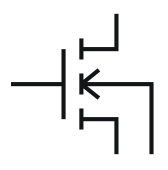
\includegraphics{nmosSymbol}}
{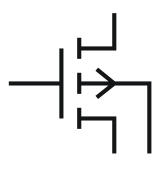
\includegraphics{pmosSymbol}}

\device
\begin{alltt}
M<name> <drain node> <gate node> <source node>
+ <bulk/substrate node> <model name>
+ [L=<value>] [W=<value>]
+ [AD=<value>] [AS=<value>]
+ [PD=<value>] [PS=<value>]
+ [NRD=<value>] [NRS=<value>]
+ [M=<value] [IC=<value, ...>]
\end{alltt}

\vbox{\hrulefill}
\item[Special Form (BSIMSOI)]
\begin{alltt}
M<name> <drain node> <gate node> <source node>
+ <substrate node (E)>
+ [<External body contact (P)>]
+ [<internal body contact (B)>]
+ [<temperature node (T)>]
+ <model name>
+ [L=<value>] [W=<value>]
+ [AD=<value>] [AS=<value>]
+ [PD=<value>] [PS=<value>]
+ [NRD=<value>] [NRS=<value>] [NRB=<value>]
+ [BJTOFF=<value>]
+ [IC=<val>,<val>,<val>,<val>,<val>]
+ [RTH0=<val>] [CTH0=<val>]
+ [NBC=<val>] [NSEG=<val>] [PDBCP=<val>] [PSBCP=<val>]
+ [AGBCP=<val>] [AEBCP=<val>] [VBSUSR=<val>] [TNODEOUT]
+ [FRBODY=<val>] [M=<value>]
\end{alltt}
\vbox{\hrulefill}

\item[Special Form (MVS)]
\begin{alltt}
M<name> <drain node> <gate node> <source node> <model name>
\end{alltt}

\item[Special Form (PSP103 with self-heating)]
\begin{alltt}
M<name> <drain node> <gate node> <source node> <bulk node> <dt node> <model name> [instance parameters]
\end{alltt}

\model
\begin{alltt}
.MODEL <model name> NMOS [model parameters]
.MODEL <model name> PMOS [model parameters]
\end{alltt}

\examples
\begin{alltt}
M5 4 12 3 0 PNOM L=20u W=10u
M3 5 13 10 0 PSTRONG
M6 7 13 10 0 PSTRONG M=2
M8 10 12 100 100 NWEAK L=30u W=20u
+ AD=288p AS=288p PD=60u PS=60u NRD=14 NRS=24
\end{alltt}

\parameters

\begin{Parameters}

\param{\vbox{\hbox{L\hfil}\hbox{M\hfil}}}

The MOSFET channel length and width that are decreased to get the actual
channel length and width. They may be given in the device
\texttt{.MODEL} or \texttt{.OPTIONS} statements. The value in the device
statement overrides the value in the model statement, which overrides
the value in the \texttt{.OPTIONS} statement. If \texttt{L} or \texttt{W}
values are not given, their default value is 100~$\mu$m.

\param{\vbox{\hbox{AD\hfil}\hbox{AS\hfil}}}

The drain and source diffusion areas. Defaults for \texttt{AD} and
\texttt{AS} can be set in the \texttt{.OPTIONS} statement.  If
\texttt{AD} or \texttt{AS} defaults are not set, their default value is
0.

\param{\vbox{\hbox{PD\hfil}\hbox{PS\hfil}}}
The drain and source diffusion perimeters. Their default value is 0.

\param{\vbox{\hbox{NRD\hfil}\hbox{NRS\hfil}}}

Multipliers (in units of $\Box$) that can be multiplied by \texttt{RSH}
to yield the parasitic (ohmic) resistances of the drain (\texttt{RD})
and source (\texttt{RS}), respectively.  \texttt{NRD}, \texttt{NRS}
default to 0.

Consider a square sheet of resistive material. Analysis shows that the
resistance between two parallel edges of such a sheet depends upon its
composition and thickness, but is independent of its size as long as it is
square. In other words, the resistance will be the same whether the square's
edge is 2~mm, 2~cm, or 2~m. For this reason, the \emph{sheet resistance} of
such a layer, abbreviated \texttt{RSH}, has units of Ohms per square,
written $\mathsf{\Omega}/\Box$.

\param{M}

If specified, the value is used as a number of parallel MOSFETs to be
simulated.  For example, if \texttt{M=2} is specified, \Xyce{} simulates two
identical mosfets connected to the same nodes in parallel.

\param{IC}

The BSIM3 (model level 9), BSIM4 (model level 14 or 54) and BSIMSOI (model
level 10) allow one to specify the initial voltage difference across
nodes of the device during the DC operating point calculation.  For the
BSIM3 and BSIM4 the syntax is \texttt{IC=$V_{ds}, V_{gs}, V_{bs}$}
where $V_{ds}$ is the voltage difference between the drain and source,
$V_{gs}$ is the voltage difference between the gate and source and
$V_{bs}$ is the voltage difference between the body and source.  The
BSIMSOI device's initial condition syntax is \texttt{IC=$V_{ds},
  V_{gs}, V_{bs}, V_{es}, V_{ps}$} where the two extra terms are the
voltage difference between the substrate and source, and the external
body and source nodes respectively.  Note that for any of these lists of
voltage differences, fewer than the full number of options may be
specified.  For example, \texttt{IC=5.0} specifies an initial condition on $V_{ds}$
but does not specifiy any initial conditions on the other nodes.
Therefore, one cannot specify $V_{gs}$ without specifying $V_{ds}$, etc.

It is illegal to specify initial conditions on any nodes that are tied
together.  \Xyce{} attempts to catch such errors, but complex circuits may
stymie this error trap.

\end{Parameters}

\vbox{\hrulefill}
\item[BSIM-SOI Options]

There are a large number of extra instance parameters and optional
nodes available for the BSIM-SOI (level 10 (BSIM-SOI 3.2), level 70
(BSIM-SOI 4.6.1), and level 70450 (BSIM-SOI 4.5.0)) MOSFET.  Please
consult the BSIM-SOI technical manual, available at
\url{http://bsim.berkeley.edu/models/bsimsoi/}, for full details.

\begin{Parameters}

\param{substrate node}

The fourth node of the BSIM-SOI device is always the substrate node,
which is referred to as the \texttt{E} node. 

\param{external body contact node}

If given, the fifth node is the external body contact node,
\texttt{P}.  It is connected to the internal body node through a body
tie resistor.  If \texttt{P} is not given, the internal body node is
not accessible from the netlist and floats.

{\em For the BSIM-SOI 3.2 (level=10) only):} If there are only five
nodes specified and \texttt{TNODEOUT} is also specified, the fifth
node is the temperature node instead.

\param{internal body contact node}

If given, the sixth node is the internal body contact node, \texttt{B}.  It is
connected to the external body node through a body tie resistor.  If \texttt{B}
is not given and \texttt{P} is given, the internal body node is not accessible
from the netlist, but is still tied to the external body contact through the
tie resistance.

{\em For the BSIM-SOI 3.2 (level=10) only):} If there are only six
nodes specified and \texttt{TNODEOUT} is also specified, the sixth
node is the temperature node instead.

\param{temperature node}

{\em For the BSIM-SOI 3.2 (level=10) only):} If the parameter \texttt{TNODEOUT} is specified, the final node (fifth, sixth,
or seventh) is interpreted as a temperature node.  The temperature node is
intended for thermal coupling simulation.

{\em For the BSIM-SOI 4.x (level=70 or 70450) only):} The temperature
node is only accessible for thermal coupling if it is the seventh
node.  It is available for printing as an internal node in all other
configurations.

\param{BJTOFF}
Turns off the parasitic BJT currents.

\param{IC}
The \texttt{IC} parameter allows specification of the five junction initial
conditions, $V_{ds}, V_{gs}, V_{bs}, V_{es}$ and $V_{ps}$.  $V_{ps}$ is ignored
in a four-terminal device.

\param{RTH0}
Thermal resistance per unit width.  Taken from model card if not given.

\param{CTH0}
Thermal capacitance per unit width.  Taken from model card if not given.

\param{NBC}
Number of body contact isolation edges.

\param{NSEG}
Number of segments for channel width partitioning.

\param{PDBCP}
Parasitic perimeter length for body contact at drain side.

\param{PSBCP}
Parasitic perimeter length for body contact at source side.

\param{AGBCP}
Parasitic gate-to-body overlap area for body contact.

\param{AEBCP}
Parasitic body-to-substrate overlap area for body contact.

\param{VBSUSR}
Optional initial value of VBS specified by user for use in transient
analysis.  (unused in \Xyce{}).

\param{FRBODY}
Layout-dependent body resistance coefficient.

\end{Parameters}

\comments

The simulator provides multiple MOSFET device models, which differ in the
formulation of the I-V characteristic. The \texttt{LEVEL} parameter
selects among different models as shown below.

For HSPICE compatibility, the BSIM4 model can be specified with either
level 14 or level 54.

If a model supports parameter aliases (e.g. ``U0'' and ``UO'' or
``VT0'' and ``VTO'' in the levels 1-6 MOSFETS), it would be a mistake
to specify both parameters and give them different values.  There is
no warning or error message if you do that.  Don't do that.

\end{Device}

\paragraph{MOSFET Operating Temperature}
Model parameters may be assigned unique measurement temperatures using the
\textrmb{TNOM} model parameter. See the MOSFET model parameters for more
information.

\paragraph{MOSFET Power Calculations}
Power dissipated in the transistor is calculated with $I_{D}*V_{DS}+I_{G}*V_{GS}$ where
$I_{D}$ is the drain current, $I_{G}$ is the gate current, $V_{DS}$ is the
voltage drop between the drain and the source and $V_{GS}$ is the voltage drop
between the gate and the source. This formula may differ from other simulators,
such as HSPICE and PSpice.

\paragraph{Internal Device Variables Accessible with {\tt N()} Syntax}
For the BSIM3, BSIM4, and BSIM-CMG version 110 models, several
internal variables have been made accessible with the {\tt N()} syntax
on a {\tt .PRINT} line.  They are $g_{m}$ (tranconductance), $V_{th}$,
$V_{ds}$, $V_{gs}$, $V_{bs}$, and $V_{dsat}$.  An example {\tt .PRINT}
line command for a MOSFET device named {\tt m1} would be:
\begin{alltt}
.print dc N(m1:gm) N(m1:Vth) N(m1:Vdsat) N(m1:Vds) N(m1:Vgs) N(m1:Vbs)
\end{alltt}
The BSIM-CMG also supports output of $I_{ds}$ (drain-source current)
in this manner.

If the user runs \texttt{Xyce -namesfile <filename> <netlist>} then
\Xyce{} will output into the first filename a list of all solution
variables generated by that netlist. This can be useful for
determining the ``fully-qualified'' device name, needed for the {\tt
  N()} syntax, if the device is in a subcircuit.

\paragraph{Instance Parameters}
Tables ~\ref{M_1_Device_Instance_Params}, ~\ref{M_2_Device_Instance_Params}, 
~\ref{M_3_Device_Instance_Params},  ~\ref{M_6_Device_Instance_Params},
\ref{M_9_Device_Instance_Params} and \ref{M_10_Device_Instance_Params}  
give the available instance parameters for the levels 1,2,3,6,9 and 10 MOSFETs,
respectively.

In addition to the parameters shown in the tables, where a list of
numbered initial condition parameters are shown, the MOSFETs support a vector
parameter for the initial conditions.  \texttt{IC1} and \texttt{IC2}
may therefore be specified compactly as \texttt{IC=<ic1>,<ic2>}.

\paragraph{Model Parameters}
Tables ~\ref{M_1_Device_Model_Params}, ~\ref{M_2_Device_Model_Params},
~\ref{M_3_Device_Model_Params}, ~\ref{M_6_Device_Model_Params},
~\ref{M_9_Device_Model_Params}, and ~\ref{M_10_Device_Model_Params}
give the available model parameters for the levels 1,2,3,6,9 and 10 MOSFETs,
respectively.

For a thorough description of MOSFET models see~\cite{Antognetti:1988, HLJHCKH,
BLETK:1997, SH:1968, VL:1980,
SSKJ:1987, Pierret:1984, YEC:1983, BSIM3:V3:1, BN}.

\subparagraph{All MOSFET models}
The parameters shared by all MOSFET model levels are principally parasitic
element values (e.g., series resistance, overlap capacitance, etc.).

\subparagraph{Model levels 1 and 3}
The DC behaviors of the level 1 and 3 MOSFET models are defined by the
parameters \textrmb{VTO}, \textrmb{KP}, \textrmb{LAMBDA}, \textrmb{PHI}, and
\textrmb{GAMMA}.  The simulator calculates these if the process parameters
(e.g., \textrmb{TOX}, and \textrmb{NSUB}) are specified, but these are always
overridden by any user-defined values. The \textrmb{VTO} value is positive
(negative) for modeling the enhancement mode and negative (positive) for the
depletion mode of N-channel (P-channel) devices.

For MOSFETs, the capacitance model enforces charge conservation,
influencing just the Level 1 and 3 models.

Effective device parameter lengths and widths are calculated as follows:
\[
P_i = P_0 + P_L / L_e + P_W / W_e
\]
where
\[
\begin{array}{rclcl}
L_e & = & \mbox{effective length} & = & \mathbf{L} - (2 \cdot \mathbf{LD}) \\
W_e & = & \mbox{effective width} & = & \mathbf{W} - (2 \cdot \mathbf{WD})
\end{array}
\]

See \textrmb{.MODEL} (model definition) for more information.

\subparagraph{Model level 9 (BSIM3 version 3.2.2)}
The University of California, Berkeley BSIM3 model is a physical-based model
with a large number of dependencies on essential dimensional and processing
parameters.  It incorporates the key effects that are critical in modeling
deep-submicrometer MOSFETs.  These include threshold voltage reduction,
nonuniform doping, mobility reduction due to the vertical field, bulk charge
effect, carrier velocity saturation, drain-induced barrier lowering (DIBL),
channel length modulation (CLM), hot-carrier-induced output resistance
reduction, subthreshold conduction, source/drain parasitic resistance,
substrate current induced body effect (SCBE) and drain voltage reduction in LDD
structure.

The BSIM3 Version 3.2.2 model is a deep submicron MOSFET model with several major
enhancements over earlier versions.  These include a single I-V formula used
to define the current and output conductance for operating regions, improved
narrow width device modeling, a superior capacitance model with improved short
and narrow geometry models, a new relaxation-time model to better transient
modeling and enhanced model fitting of assorted W/L ratios using a single
parameter set.  This version preserves the large number of integrated
dependencies on dimensional and processing parameters of the Version 2 model.
For further information, see Reference~\cite{HLJHCKH}.

\subparagraph{Additional notes}
\begin{enumerate}
\item If any of the following BSIM3 3.2.2 model parameters are not specified,
they are computed via the following:

If \textrmb{VTHO} is not specified, then:
\[
\mathbf{VTHO} = \mathbf{VFB} + \phi_s \mathbf{K1} \sqrt{\phi_s}
\]
where:
\[
\mathbf{VFB} = -1.0
\]
If \textrmb{VTHO} is given, then:
\begin{eqnarray*}
\mathbf{VFB} & = & \mathbf{VTHO} - \phi_s + \mathbf{K1}\sqrt{phi_s} \\
\mathbf{VBX} & = & \phi_s - \frac{q\cdot\mathbf{NCH} \cdot
\mathbf{XT}^2}{2\varepsilon_{si}} \\
\mathbf{CF} & = & \left( \frac{2\varepsilon_{ox}}{\pi} \right)
\ln \left(1 + \frac{1}{4 \times 10^7\cdot\mathbf{TOX}} \right)
\end{eqnarray*}
where:
\[
E_g(T) = \mbox{the energy bandgap at temperature }T = 1.16 - \frac{T^2}{7.02
\times 10^4(T + 1108)}
\]

\item If \textrmb{K1} and \textrmb{K2} are not given then they are computed via
the following:
\begin{eqnarray*}
\mathbf{K1} &=& \mathbf{GAMMA2} - 2 \cdot \mathbf{K2} \sqrt{\phi_s -
\mathbf{VBM}} \\
\mathbf{K2} &=& \frac{(\mathbf{GAMMA1} -
\mathbf{GAMMA2})(\sqrt{\phi_s - \mathbf{VBX}} -
\sqrt{\phi_s})}{2\sqrt{\phi_s}(\sqrt{\phi_s - \mathbf{VBM}} -
\sqrt{\phi_s}) + \mathbf{VBM}}
\end{eqnarray*}
where:
\begin{eqnarray*}
\phi_s & = & 2V_t \ln \left(\frac{\mathbf{NCH}}{n_i} \right) \\
V_t    & = & kT / q \\
n_i    & = & 1.45 \times 10^{10} \left(\frac{T}{300.15}
\right)^{1.5} \exp \left(21.5565981 - \frac{E_g(T)}{2V_t} \right)
\end{eqnarray*}

\item If \textrmb{NCH} is not specified and \textrmb{GAMMA1} is, then:
\[
\mathbf{NCH} = \frac{\mathbf{GAMMA1^2 \times \mathbf{COX}^2}}
{2q \varepsilon_{si}}
\]
If \textrmb{GAMMA1} and \textrmb{NCH} {\em are not} specified, then
\textrmb{NCH} defaults to $1.7\times10^{23}\;m^{-3}$ and \textrmb{GAMMA1} is
computed using \textrmb{NCH}:
\[
\mathbf{GAMMA1} = \frac{\sqrt{2q\varepsilon_{si} \cdot \mathbf{NCH}}}
{\mathbf{COX}}
\]
If \textrmb{GAMMA2} is not specified, then:
\[
\mathbf{GAMMA2} = \frac{\sqrt{2q\varepsilon_{si} \cdot \mathbf{NSUB}}}
{\mathbf{COX}}
\]

\item If \textrmb{CGSO} is not specified and $\mathbf{DLC} > 0$, then:
\[
\mathbf{CGSO} = \left\{ \begin{array}{ll}
0, & ((\mathbf{DLC \cdot COX) - CGSL)} < 0        \\
0.6 \cdot \mathbf{XJ \cdot COX}, & ((\mathbf{DLC \cdot COX) - CGSL)}
\geq 0
\end{array}
\right.
\]

\item If \textrmb{CGDO} is not specified and $\mathbf{DLC} > 0$, then:
\[
\mathbf{CGDO} = \left\{ \begin{array}{ll}
0, & ((\mathbf{DLC \cdot COX) - CGSL)} < 0 \\
0.6 \cdot \mathbf{XJ \cdot COX},
& ((\mathbf{DLC \cdot COX) - CGSL)} \geq 0
\end{array}
\right. \]
\end{enumerate}

\subparagraph{Model level 10 (BSIM-SOI version 3.2)}

The BSIM-SOI is an international standard model for SOI (silicon on insulator)
circuit design and is formulated on top of the BSIM3v3 framework.
A detailed description can be found in the BSIM-SOI 3.1 User's
Manual~\cite{BSIMSOI:Manual} and the BSIM-SOI 3.2 release
notes~\cite{BSIMSOI:3p2:Notes}.

This version (v3.2) of the BSIM-SOI includes three depletion models;
the partially depleted BSIM-SOI PD (soiMod=0), the fully depleted BSIM-SOI
FD (soiMod=2), and the unified SOI model (soiMod=1).

BSIMPD is the
Partial-Depletion (PD) mode of the BSIM-SOI.  A typical PD SOI MOSFET is formed
on a thin SOI film which is layered on top of a buried oxide.  BSIMPD has
the following features and enhancements:
\begin{XyceItemize}
\item Real floating body simulation of both I-V and C-V.  The body potential is
      determined by the balance of all body current components.
\item An improved parasitic bipolar current model.  This includes enhancements in
      the various diode leakage components, second order effects (high-level
      injection and Early effect), diffusion charge equation, and temperature
      dependence of the diode junction capacitance.
\item An improved impact-ionization current model.  The contribution from BJT
      current is also modeled by the parameter Fbjtii.
\item A gate-to-body tunneling current model, which is important to thin-oxide
      SOI technologies.
\item Enhancements in the threshold voltage and bulk charge formulation of the
      high positive body bias regime.
\item Instance parameters (Pdbcp, Psbcp, Agbcp, Aebcp, Nbc) are provided to model
      the parasitics of devices with various body-contact and isolation structures.
\item An external body node (the 6th node) and other improvements are introduced
      to facilitate the modeling of distributed body resistance.
\item Self heating.  An external temperature node (the 7th node) is supported to
      facilitate the simulation of thermal coupling among neighboring devices.
\item A unique SOI low frequency noise model, including a new excess noise resulting
      from the floating body effect.
\item Width dependence of the body effect is modeled by parameters (K1,K1w1,K1w2).
\item Improved history dependence of the body charges with two new parameters
      (Fbody, DLCB).
\item An instance parameter Vbsusr is provided for users to set the transient initial
      condition of the body potential.
\item The new charge-thickness capacitance model introduced in BSIM3v3.2,
      \texttt{capMod=3}, is included.
\end{XyceItemize}

\paragraph{Quadratic Temperature Compensation}
SPICE temperature effects are the default, but MOSFET levels 18, 19 and 20 have
a more advanced temperature compensation available.  By specifying
\texttt{TEMPMODEL=QUADRATIC} in the netlist, parameters can be interpolated
quadratically between measured values extracted from data.  See
Section~\ref{Model_Interpolation} for more details.

\paragraph{MOSFET Equations}
The following equations define an N-channel MOSFET. The P-channel
devices use a reverse the sign for all voltages and currents.  The
equations use the following variables:
\begin{eqnarray*}
V_{bs}  &=&\mbox{intrinsic substrate-intrinsic source voltage} \\
V_{bd}  &=&\mbox{intrinsic substrate-intrinsic drain voltage} \\
V_{ds}  &=&\mbox{intrinsic drain-substrate source voltage} \\
V_{dsat}&=&\mbox{saturation voltage} \\
V_{gs}  &=&\mbox{intrinsic gate-intrinsic source voltage} \\
V_{gd}  &=&\mbox{intrinsic gate-intrinsic drain voltage} \\
V_t     &=&kT / q \mbox{ (thermal voltage)} \\
V_{th}  &=&\mbox{threshold voltage} \\
C_{ox}  &=&\mbox{the gate oxide capacitance per unit area} \\
f       &=&\mbox{noise frequency} \\
k       &=&\mbox{Boltzmann's constant} \\
q       &=&\mbox{electron charge} \\
Leff    &=&\mbox{effective channel length} \\
Weff    &=&\mbox{effective channel width} \\
T       &=&\mbox{analysis temperature (K)} \\
T_0     &=&\mbox{nominal temperature (set using TNOM option)}
\end{eqnarray*}
Other variables are listed in the BJT Equations section~\ref{bjt_equations}.

\clearpage
\LTXtable{\textwidth}{mosfeteqntbl}

%%
%% MOSFET Equation Capacitance Table
%%
\paragraph{Capacitance}
\LTXtable{\textwidth}{mosfeteqncaptbl}

%%
%% MOSFET Equation Temperature Effects
%%
\clearpage
\paragraph{Temperature Effects}
\LTXtable{\textwidth}{mosfeteqntemptbl}

%%
%% MOSFET Parameters Table
%%
\clearpage
\subsubsection{Level 1 MOSFET Tables (SPICE Level 1)}
% This table was generated by Xyce:
%   Xyce -doc M 1
%
\index{mosfet level 1!device instance parameters}
\begin{DeviceParamTableGenerated}{MOSFET level 1 Device Instance Parameters}{M_1_Device_Instance_Params}
AD & Drain diffusion area & m$^{2}$ & 0 \\ \hline
AS & Source diffusion area & m$^{2}$ & 0 \\ \hline
DTEMP & Device delta temperature & $^\circ$C & 0 \\ \hline
IC1 & Initial condition on Drain-Source voltage & V & 0 \\ \hline
IC2 & Initial condition on Gate-Source voltage & V & 0 \\ \hline
IC3 & Initial condition on Bulk-Source voltage & V & 0 \\ \hline
L & Channel length & m & 0 \\ \hline
M & Multiplier for M devices connected in parallel & -- & 1 \\ \hline
NRD & Multiplier for RSH to yield parasitic resistance of drain & $\Box$ & 1 \\ \hline
NRS & Multiplier for RSH to yield parasitic resistance of source & $\Box$ & 1 \\ \hline
OFF & Initial condition of no voltage drops across device & logical (T/F) & false \\ \hline
PD & Drain diffusion perimeter & m & 0 \\ \hline
PS & Source diffusion perimeter & m & 0 \\ \hline
TEMP & Device temperature & $^\circ$C & Ambient Temperature \\ \hline
W & Channel width & m & 0 \\ \hline
\end{DeviceParamTableGenerated}

% This table was generated by Xyce:
%   Xyce -doc M 1
%
\index{mosfet level 1!device model parameters}
\begin{DeviceParamTableGenerated}{MOSFET level 1 Device Model Parameters}{M_1_Device_Model_Params}
AF & Flicker noise exponent & -- & 1 \\ \hline
CBD & Zero-bias bulk-drain p-n capacitance & F & 0 \\ \hline
CBS & Zero-bias bulk-source p-n capacitance & F & 0 \\ \hline
CGBO & Gate-bulk overlap capacitance/channel length & F/m & 0 \\ \hline
CGDO & Gate-drain overlap capacitance/channel width & F/m & 0 \\ \hline
CGSO & Gate-source overlap capacitance/channel width & F/m & 0 \\ \hline
CJ & Bulk p-n zero-bias bottom capacitance/area & F/m$^{2}$ & 0 \\ \hline
CJSW & Bulk p-n zero-bias sidewall capacitance/area & F/m$^{2}$ & 0 \\ \hline
FC & Bulk p-n forward-bias capacitance coefficient & -- & 0.5 \\ \hline
GAMMA & Bulk threshold parameter & V$^{1/2}$ & 0 \\ \hline
IS & Bulk p-n saturation current & A & 1e-14 \\ \hline
JS & Bulk p-n saturation current density & A/m$^{2}$ & 0 \\ \hline
KF & Flicker noise coefficient & -- & 0 \\ \hline
KP & Transconductance coefficient & A/V$^{2}$ & 2e-05 \\ \hline
L & Default channel length & m & 0.0001 \\ \hline
LAMBDA & Channel-length modulation & V$^{-1}$ & 0 \\ \hline
LD & Lateral diffusion length & m & 0 \\ \hline
MJ & Bulk p-n bottom grading coefficient & -- & 0.5 \\ \hline
MJSW & Bulk p-n sidewall grading coefficient & -- & 0.5 \\ \hline
NSS & Surface state density & cm$^{-2}$ & 0 \\ \hline
NSUB & Substrate doping density & cm$^{-3}$ & 0 \\ \hline
PB & Bulk p-n bottom potential & V & 0.8 \\ \hline
PHI & Surface potential & V & 0.6 \\ \hline
RD & Drain ohmic resistance & $\mathsf{\Omega}$ & 0 \\ \hline
RS & Source ohmic resistance & $\mathsf{\Omega}$ & 0 \\ \hline
RSH & Drain,source diffusion sheet resistance & $\mathsf{\Omega}$ & 0 \\ \hline
TNOM & Nominal device temperature & $^\circ$C & 27 \\ \hline
TOX & Gate oxide thickness & m & 1e-07 \\ \hline
TPG & Gate material type (-1 = same as substrate) 0 = aluminum,1 = opposite of substrate) & -- & 0 \\ \hline
U0 & Surface mobility (alias for UO) & 1/(Vcm$^{2}$s) & 600 \\ \hline
UO & Surface mobility & 1/(Vcm$^{2}$s) & 600 \\ \hline
VT0 & Zero-bias threshold voltage (alias for VTO) & V & 0 \\ \hline
VTO & Zero-bias threshold voltage & V & 0 \\ \hline
W & Default channel width & m & 0.0001 \\ \hline
\end{DeviceParamTableGenerated}

\clearpage
\subsubsection{Level 2 MOSFET Tables (SPICE Level 2)}
% This table was generated by Xyce:
%   Xyce -doc M 2
%
\index{mosfet level 2!device instance parameters}
\begin{DeviceParamTableGenerated}{MOSFET level 2 Device Instance Parameters}{M_2_Device_Instance_Params}
AD & Drain diffusion area & m$^{2}$ & 0 \\ \hline
AS & Source diffusion area & m$^{2}$ & 0 \\ \hline
DTEMP & Device delta temperature & $^\circ$C & 0 \\ \hline
IC1 & Initial condition on Drain-Source voltage & V & 0 \\ \hline
IC2 & Initial condition on Gate-Source voltage & V & 0 \\ \hline
IC3 & Initial condition on Bulk-Source voltage & V & 0 \\ \hline
L & Channel length & m & 0 \\ \hline
M & Multiplier for M devices connected in parallel & -- & 1 \\ \hline
NRD & Multiplier for RSH to yield parasitic resistance of drain & $\Box$ & 1 \\ \hline
NRS & Multiplier for RSH to yield parasitic resistance of source & $\Box$ & 1 \\ \hline
OFF & Initial condition of no voltage drops across device & logical (T/F) & false \\ \hline
PD & Drain diffusion perimeter & m & 0 \\ \hline
PS & Source diffusion perimeter & m & 0 \\ \hline
TEMP & Device temperature & $^\circ$C & Ambient Temperature \\ \hline
W & Channel width & m & 0 \\ \hline
\end{DeviceParamTableGenerated}

% This table was generated by Xyce:
%   Xyce -doc M 2
%
\index{mosfet level 2!device model parameters}
\begin{DeviceParamTableGenerated}{MOSFET level 2 Device Model Parameters}{M_2_Device_Model_Params}
AF & Flicker noise exponent & -- & 1 \\ \hline
CBD & Zero-bias bulk-drain p-n capacitance & F & 0 \\ \hline
CBS & Zero-bias bulk-source p-n capacitance & F & 0 \\ \hline
CGBO & Gate-bulk overlap capacitance/channel length & F/m & 0 \\ \hline
CGDO & Gate-drain overlap capacitance/channel width & F/m & 0 \\ \hline
CGSO & Gate-source overlap capacitance/channel width & F/m & 0 \\ \hline
CJ & Bulk p-n zero-bias bottom capacitance/area & F/m$^{2}$ & 0 \\ \hline
CJSW & Bulk p-n zero-bias sidewall capacitance/area & F/m$^{2}$ & 0 \\ \hline
DELTA & Width effect on threshold & -- & 0 \\ \hline
FC & Bulk p-n forward-bias capacitance coefficient & -- & 0.5 \\ \hline
GAMMA & Bulk threshold parameter & V$^{1/2}$ & 0 \\ \hline
IS & Bulk p-n saturation current & A & 1e-14 \\ \hline
JS & Bulk p-n saturation current density & A/m$^{2}$ & 0 \\ \hline
KF & Flicker noise coefficient & -- & 0 \\ \hline
KP & Transconductance coefficient & A/V$^{2}$ & 2e-05 \\ \hline
L & Default channel length & m & 0.0001 \\ \hline
LAMBDA & Channel-length modulation & V$^{-1}$ & 0 \\ \hline
LD & Lateral diffusion length & m & 0 \\ \hline
MJ & Bulk p-n bottom grading coefficient & -- & 0.5 \\ \hline
MJSW & Bulk p-n sidewall grading coefficient & -- & 0.5 \\ \hline
NEFF & Total channel charge coeff. & -- & 1 \\ \hline
NFS & Fast surface state density & -- & 0 \\ \hline
NSS & Surface state density & cm$^{-2}$ & 0 \\ \hline
NSUB & Substrate doping density & cm$^{-3}$ & 0 \\ \hline
PB & Bulk p-n bottom potential & V & 0.8 \\ \hline
PHI & Surface potential & V & 0.6 \\ \hline
RD & Drain ohmic resistance & $\mathsf{\Omega}$ & 0 \\ \hline
RS & Source ohmic resistance & $\mathsf{\Omega}$ & 0 \\ \hline
RSH & Drain,source diffusion sheet resistance & $\mathsf{\Omega}$ & 0 \\ \hline
TNOM & Nominal device temperature & $^\circ$C & 27 \\ \hline
TOX & Gate oxide thickness & m & 1e-07 \\ \hline
TPG & Gate material type (-1 = same as substrate, 0 = aluminum,1 = opposite of substrate) & -- & 0 \\ \hline
U0 & Surface mobility (alias for UO) & 1/(Vcm$^{2}$s) & 600 \\ \hline
UCRIT & Crit. field for mob. degradation & -- & 10000 \\ \hline
UEXP & Crit. field exp for mob. deg. & -- & 0 \\ \hline
UO & Surface mobility & 1/(Vcm$^{2}$s) & 600 \\ \hline
VMAX & Maximum carrier drift velocity & -- & 0 \\ \hline
VT0 & Zero-bias threshold voltage (alias for VTO) & V & 0 \\ \hline
VTO & Zero-bias threshold voltage & V & 0 \\ \hline
W & Default channel width & m & 0.0001 \\ \hline
XJ & Junction depth & -- & 0 \\ \hline
\end{DeviceParamTableGenerated}

\clearpage
\subsubsection{Level 3 MOSFET Tables (SPICE Level 3)}
% This table was generated by Xyce:
%   Xyce -doc M 3
%
\index{mosfet level 3!device instance parameters}
\begin{DeviceParamTableGenerated}{MOSFET level 3 Device Instance Parameters}{M_3_Device_Instance_Params}
AD & Drain diffusion area & m$^{2}$ & 0 \\ \hline
AS & Source diffusion area & m$^{2}$ & 0 \\ \hline
DTEMP & Device delta temperature & $^\circ$C & 0 \\ \hline
IC1 & Initial condition on Drain-Source voltage & V & 0 \\ \hline
IC2 & Initial condition on Gate-Source voltage & V & 0 \\ \hline
IC3 & Initial condition on Bulk-Source voltage & V & 0 \\ \hline
L & Channel length & m & 0 \\ \hline
M & Multiplier for M devices connected in parallel & -- & 1 \\ \hline
NRD & Multiplier for RSH to yield parasitic resistance of drain & $\Box$ & 1 \\ \hline
NRS & Multiplier for RSH to yield parasitic resistance of source & $\Box$ & 1 \\ \hline
OFF & Initial condition of no voltage drops across device & logical (T/F) & false \\ \hline
PD & Drain diffusion perimeter & m & 0 \\ \hline
PS & Source diffusion perimeter & m & 0 \\ \hline
TEMP & Device temperature & $^\circ$C & Ambient Temperature \\ \hline
W & Channel width & m & 0 \\ \hline
\end{DeviceParamTableGenerated}

% This table was generated by Xyce:
%   Xyce -doc M 3
%
\index{mosfet level 3!device model parameters}
\begin{DeviceParamTableGenerated}{MOSFET level 3 Device Model Parameters}{M_3_Device_Model_Params}
AF & Flicker noise exponent & -- & 1 \\ \hline
CBD & Zero-bias bulk-drain p-n capacitance & F & 0 \\ \hline
CBS & Zero-bias bulk-source p-n capacitance & F & 0 \\ \hline
CGBO & Gate-bulk overlap capacitance/channel length & F/m & 0 \\ \hline
CGDO & Gate-drain overlap capacitance/channel width & F/m & 0 \\ \hline
CGSO & Gate-source overlap capacitance/channel width & F/m & 0 \\ \hline
CJ & Bulk p-n zero-bias bottom capacitance/area & F/m$^{2}$ & 0 \\ \hline
CJSW & Bulk p-n zero-bias sidewall capacitance/area & F/m$^{2}$ & 0 \\ \hline
DELTA & Width effect on threshold & -- & 0 \\ \hline
ETA & Static feedback & -- & 0 \\ \hline
FC & Bulk p-n forward-bias capacitance coefficient & -- & 0.5 \\ \hline
GAMMA & Bulk threshold parameter & V$^{1/2}$ & 0 \\ \hline
IS & Bulk p-n saturation current & A & 1e-14 \\ \hline
JS & Bulk p-n saturation current density & A/m$^{2}$ & 0 \\ \hline
KAPPA & Saturation field factor & -- & 0.2 \\ \hline
KF & Flicker noise coefficient & -- & 0 \\ \hline
KP & Transconductance coefficient & A/V$^{2}$ & 2e-05 \\ \hline
L & Default channel length & m & 0.0001 \\ \hline
LD & Lateral diffusion length & m & 0 \\ \hline
MJ & Bulk p-n bottom grading coefficient & -- & 0.5 \\ \hline
MJSW & Bulk p-n sidewall grading coefficient & -- & 0.33 \\ \hline
NFS & Fast surface state density & cm$^{-2}$ & 0 \\ \hline
NSS & Surface state density & cm$^{-2}$ & 0 \\ \hline
NSUB & Substrate doping density & cm$^{-3}$ & 0 \\ \hline
PB & Bulk p-n bottom potential & V & 0.8 \\ \hline
PHI & Surface potential & V & 0.6 \\ \hline
RD & Drain ohmic resistance & $\mathsf{\Omega}$ & 0 \\ \hline
RS & Source ohmic resistance & $\mathsf{\Omega}$ & 0 \\ \hline
RSH & Drain,source diffusion sheet resistance & $\mathsf{\Omega}$ & 0 \\ \hline
THETA & Mobility modulation & V$^{-1}$ & 0 \\ \hline
TNOM & Nominal device temperature & $^\circ$C & 27 \\ \hline
TOX & Gate oxide thickness & m & 1e-07 \\ \hline
TPG & Gate material type (-1 = same as substrate,0 = aluminum,1 = opposite of substrate) & -- & 1 \\ \hline
U0 & Surface mobility (alias for UO) & 1/(Vcm$^{2}$s) & 600 \\ \hline
UO & Surface mobility & 1/(Vcm$^{2}$s) & 600 \\ \hline
VMAX & Maximum drift velocity & m/s & 0 \\ \hline
VT0 & Zero-bias threshold voltage (alias for VTO) & V & 0 \\ \hline
VTO & Zero-bias threshold voltage & V & 0 \\ \hline
W & Default channel width & m & 0.0001 \\ \hline
XJ & Metallurgical junction depth & m & 0 \\ \hline
\end{DeviceParamTableGenerated}

\clearpage
\subsubsection{Level 6 MOSFET Tables (SPICE Level 6)}
% This table was generated by Xyce:
%   Xyce -doc M 6
%
\index{mosfet level 6!device instance parameters}
\begin{DeviceParamTableGenerated}{MOSFET level 6 Device Instance Parameters}{M_6_Device_Instance_Params}
AD & Drain diffusion area & m$^{2}$ & 0 \\ \hline
AS & Source diffusion area & m$^{2}$ & 0 \\ \hline
DTEMP & Device delta temperature & $^\circ$C & 0 \\ \hline
IC1 & Initial condition on Drain-Source voltage & V & 0 \\ \hline
IC2 & Initial condition on Gate-Source voltage & V & 0 \\ \hline
IC3 & Initial condition on Bulk-Source voltage & V & 0 \\ \hline
L & Channel length & m & 0 \\ \hline
M & Multiplier for M devices connected in parallel & -- & 1 \\ \hline
NRD & Multiplier for RSH to yield parasitic resistance of drain & $\Box$ & 1 \\ \hline
NRS & Multiplier for RSH to yield parasitic resistance of source & $\Box$ & 1 \\ \hline
OFF & Initial condition of no voltage drops across device & logical (T/F) & false \\ \hline
PD & Drain diffusion perimeter & m & 0 \\ \hline
PS & Source diffusion perimeter & m & 0 \\ \hline
TEMP & Device temperature & $^\circ$C & Ambient Temperature \\ \hline
W & Channel width & m & 0 \\ \hline
\end{DeviceParamTableGenerated}

% This table was generated by Xyce:
%   Xyce -doc M 6
%
\index{mosfet level 6!device model parameters}
\begin{DeviceParamTableGenerated}{MOSFET level 6 Device Model Parameters}{M_6_Device_Model_Params}
AF & Flicker noise exponent & -- & 1 \\ \hline
CBD & Zero-bias bulk-drain p-n capacitance & F & 0 \\ \hline
CBS & Zero-bias bulk-source p-n capacitance & F & 0 \\ \hline
CGBO & Gate-bulk overlap capacitance/channel length & F/m & 0 \\ \hline
CGDO & Gate-drain overlap capacitance/channel width & F/m & 0 \\ \hline
CGSO & Gate-source overlap capacitance/channel width & F/m & 0 \\ \hline
CJ & Bulk p-n zero-bias bottom capacitance/area & F/m$^{2}$ & 0 \\ \hline
CJSW & Bulk p-n zero-bias sidewall capacitance/area & F/m$^{2}$ & 0 \\ \hline
FC & Bulk p-n forward-bias capacitance coefficient & -- & 0.5 \\ \hline
GAMMA & Bulk threshold parameter & -- & 0 \\ \hline
GAMMA1 & Bulk threshold parameter 1 & -- & 0 \\ \hline
IS & Bulk p-n saturation current & A & 1e-14 \\ \hline
JS & Bulk p-n saturation current density & A/m$^{2}$ & 0 \\ \hline
KC & Saturation current factor & -- & 5e-05 \\ \hline
KF & Flicker noise coefficient & -- & 0 \\ \hline
KV & Saturation voltage factor & -- & 2 \\ \hline
LAMBDA & Channel length modulation param. & -- & 0 \\ \hline
LAMBDA0 & Channel length modulation param. 0 & -- & 0 \\ \hline
LAMBDA1 & Channel length modulation param. 1 & -- & 0 \\ \hline
LD & Lateral diffusion length & m & 0 \\ \hline
MJ & Bulk p-n bottom grading coefficient & -- & 0.5 \\ \hline
MJSW & Bulk p-n sidewall grading coefficient & -- & 0.5 \\ \hline
NC & Saturation current coeff. & -- & 1 \\ \hline
NSS & Surface state density & cm$^{-2}$ & 0 \\ \hline
NSUB & Substrate doping density & cm$^{-3}$ & 0 \\ \hline
NV & Saturation voltage coeff. & -- & 0.5 \\ \hline
NVTH & Threshold voltage coeff. & -- & 0.5 \\ \hline
PB & Bulk p-n bottom potential & V & 0.8 \\ \hline
PHI & Surface potential & V & 0.6 \\ \hline
PS & Sat. current modification  par. & -- & 0 \\ \hline
RD & Drain ohmic resistance & $\mathsf{\Omega}$ & 0 \\ \hline
RS & Source ohmic resistance & $\mathsf{\Omega}$ & 0 \\ \hline
RSH & Drain,source diffusion sheet resistance & $\mathsf{\Omega}$ & 0 \\ \hline
SIGMA & Static feedback effect par. & -- & 0 \\ \hline
TNOM & Nominal device temperature & $^\circ$C & 27 \\ \hline
TOX & Gate oxide thickness & m & 1e-07 \\ \hline
TPG & Gate material type (-1 = same as substrate,0 = aluminum,1 = opposite of substrate) & -- & 1 \\ \hline
U0 & Surface mobility (alias for UO) & 1/(Vcm$^{2}$s) & 600 \\ \hline
UO & Surface mobility & 1/(Vcm$^{2}$s) & 600 \\ \hline
VT0 & Zero-bias threshold voltage (alias for VTO) & V & 0 \\ \hline
VTO & Zero-bias threshold voltage & V & 0 \\ \hline
\end{DeviceParamTableGenerated}

\clearpage
\subsubsection{Level 9 MOSFET Tables (BSIM3)}
For complete documentation of the BSIM3 model, see the users' manual for
the BSIM3, available for download at
\url{http://bsim.berkeley.edu/models/bsim4/bsim3/}.
\Xyce{} implements Version 3.2.2 of the BSIM3.

In addition to the parameters shown in
table~\ref{M_9_Device_Instance_Params}, the BSIM3 supports a vector
parameter for the initial conditions.  \texttt{IC1} through
\texttt{IC3} may therefore be specified compactly as
\texttt{IC=<ic1>,<ic2>,<ic3>}.

\textbf{NOTE:  Many BSIM3 parameters listed in
tables~\ref{M_9_Device_Instance_Params} and \ref{M_9_Device_Model_Params} as
having default values of zero are actually replaced with internally computed
defaults if not given.  Specifying zero in your model card will override this
internal computation.  It is recommended that you only set model parameters
that you are actually changing from defaults and that you not generate model
cards containing default values from the tables.}
% This table was generated by Xyce:
%   Xyce -doc_cat M 9
%
\index{bsim3!device instance parameters}
\begin{DeviceParamTableGenerated}{BSIM3 Device Instance Parameters}{M_9_Device_Instance_Params}

\category{Control Parameters}\\ \hline
M & Multiplier for M devices connected in parallel & -- & 1 \\ \hline
NQSMOD & Flag for NQS model & -- & 0 \\ \hline

\category{Geometry Parameters}\\ \hline
AD & Drain diffusion area & m$^{2}$ & 0 \\ \hline
AS & Source diffusion area & m$^{2}$ & 0 \\ \hline
L & Channel length & m & 0 \\ \hline
NRD & Multiplier for RSH to yield parasitic resistance of drain & $\Box$ & 1 \\ \hline
NRS & Multiplier for RSH to yield parasitic resistance of source & $\Box$ & 1 \\ \hline
PD & Drain diffusion perimeter & m & 0 \\ \hline
PS & Source diffusion perimeter & m & 0 \\ \hline
W & Channel width & m & 0 \\ \hline

\category{Temperature Parameters}\\ \hline
TEMP & Device temperature & $^\circ$C & Ambient Temperature \\ \hline

\category{Voltage Parameters}\\ \hline
IC1 & Initial condition on Vds & V & 0 \\ \hline
IC2 & Initial condition on Vgs & V & 0 \\ \hline
IC3 & Initial condition on Vbs & V & 0 \\ \hline
OFF & Initial condition of no voltage drops accross device & logical (T/F) & false \\ \hline
\end{DeviceParamTableGenerated}

% This table was generated by Xyce:
%   Xyce -doc_cat M 9
%
\index{bsim3!device model parameters}
\begin{DeviceParamTableGenerated}{BSIM3 Device Model Parameters}{M_9_Device_Model_Params}

\category{Bin Parameters}\\ \hline
LMAX & Maximum channel length & m & 1 \\ \hline
LMIN & Minimum channel length & m & 0 \\ \hline
WMAX & Maximum channel width & m & 1 \\ \hline
WMIN & Minimum channel width & m & 0 \\ \hline

\category{Capacitance Parameters}\\ \hline
ACDE & Exponetial coefficient for charge thickness in capmod = 3 for accumulation and depletion regions & m/V & 1 \\ \hline
CF & Firing field capacitance & F/m & 0 \\ \hline
CGBO & Gate-bulk overlap capacitance per unit channel length & F/m & 0 \\ \hline
CGDL & Light-doped drain-gate region overlap capacitance & F/m & 0 \\ \hline
CGDO & Non-LLD region drain-gate overlap capacitance per unit channel length & F/m & 0 \\ \hline
CGSL & Light-doped source-gate region overlap capacitance & F/m & 0 \\ \hline
CGSO & Non-LLD region source-gate overlap capacitance per unit channel length & F/m & 0 \\ \hline
CJ & Bulk p-n zero-bias bottom capacitance/area & F/m$^{2}$ & 0.0005 \\ \hline
CJSW & Bulk p-n zero-bias sidewall capacitance/area & F/m$^{2}$ & 5e-10 \\ \hline
CJSWG & Source/grain gate sidewall junction capacitance per unit width & F/m & 0 \\ \hline
CKAPPA & Coefficient for lightly doped region overlap capacitance fireing field capacitance & F/m & 0.6 \\ \hline
CLC & Constant term for short-channel model & m & 1e-07 \\ \hline
CLE & Exponetial term for the short-channel model & -- & 0.6 \\ \hline
DLC & Length offset fitting parameter from C-V & m & 0 \\ \hline
DWC & Width offset fitting parameter from C-V & m & 0 \\ \hline
MJSWG & Source/grain gate sidewall junction capacitance grading coeficient & -- & 0 \\ \hline
MOIN & Coefficient for the gate-bias dependent surface potential & -- & 15 \\ \hline
NOFF & CV parameter in Vgsteff,CV for weak to strong inversion & -- & 1 \\ \hline
PBSW & Source/drain side junction built-in potential & V & 1 \\ \hline
PBSWG & Source/drain gate sidewall junction built-in potential & V & 0 \\ \hline
VFBCV & Flat-band voltage parameter (for CAPMOD = 0 only) & V & -1 \\ \hline
VOFFCV & CV parameter in Vgsteff,CV for weak to strong inversion & V & 0 \\ \hline
XPART & Charge partitioning rate flag & -- & 0 \\ \hline

\category{Control Parameters}\\ \hline
BINUNIT & Binning unit selector & -- & 1 \\ \hline
CAPMOD & Flag for capacitance models & -- & 3 \\ \hline
MOBMOD & Mobility model selector & -- & 1 \\ \hline
NOIMOD & Flag for noise models & -- & 1 \\ \hline
PARAMCHK & Parameter value check & -- & 0 \\ \hline
VERSION & Version number & -- & '3.2.2' \\ \hline

\category{DC Parameters}\\ \hline
A0 & Bulk charge effect coefficient for channel length & -- & 1 \\ \hline
A1 & First non-saturation effect parameter & V$^{-1}$ & 0 \\ \hline
A2 & Second non-saturation factor & -- & 1 \\ \hline
AGS & Gate-bias coefficient of abulk & V$^{-1}$ & 0 \\ \hline
ALPHA0 & First parameter of impact-ionization current & m/V & 0 \\ \hline
ALPHA1 & Isub parameter for length scaling & V$^{-1}$ & 0 \\ \hline
B0 & Bulk charge effect coefficient for channel width & m & 0 \\ \hline
B1 & Bulk charge effect offset & m & 0 \\ \hline
BETA0 & Second parameter of impact-ionization current & V & 30 \\ \hline
CDSC & Drain/source to channel coupling capacitance & F/m$^{2}$ & 0.00024 \\ \hline
CDSCB & Body-bias sensitivity of CDSC & F/(Vm$^{2}$) & 0 \\ \hline
CDSCD & Drain-bias sensitivity of CDSC & F/(Vm$^{2}$) & 0 \\ \hline
CIT & Interface trap capacitance & F/m$^{2}$ & 0 \\ \hline
DELTA & Effective Vds parameter & V & 0.01 \\ \hline
DROUT & L-depedance Coefficient of the DIBL correction parameter in Rout & -- & 0.56 \\ \hline
DSUB & DIBL coefficient exponent in subthreshhold region & -- & 0 \\ \hline
DVT0 & First coefficient of short-channel effect effect on threshold voltage & -- & 2.2 \\ \hline
DVT0W & First coefficient of narrow-width effect effect on threshold voltage for small channel length & m$^{-1}$ & 0 \\ \hline
DVT1 & Second coefficient of short-channel effect effect on threshold voltage & -- & 0.53 \\ \hline
DVT1W & Second coefficient of narrow-width effect effect on threshold voltage for small channel length & m$^{-1}$ & 5.3e+06 \\ \hline
DVT2 & Body-bias coefficient of short-channel effect effect on threshold voltage & V$^{-1}$ & -0.032 \\ \hline
DVT2W & Body-bias coefficient of narrow-width effect effect on threshold voltage for small channel length & V$^{-1}$ & -0.032 \\ \hline
DWB & Coefficient of substrate body bias dependence of Weff & m/V$^{1/2}$ & 0 \\ \hline
DWG & Coefficient of gate depedence of Weff & m/V$^{1/2}$ & 0 \\ \hline
ETA0 & DIBL coefficient in subthreshold region & -- & 0.08 \\ \hline
ETAB & Body-bias coefficient for the subthreshold DIBL effect & V$^{-1}$ & -0.07 \\ \hline
IJTH & Diode limiting current & A & 0.1 \\ \hline
JSW & Sidewall saturation current per unit length & A/m & 0 \\ \hline
K1 & First-order body effect coefficient & V$^{1/2}$ & 0 \\ \hline
K2 & second-order body effect coefficient & -- & 0 \\ \hline
K3 & Narrow width coefficient & -- & 80 \\ \hline
K3B & Body effect coefficient of K3 & V$^{-1}$ & 0 \\ \hline
KETA & Body-bias coefficient of bulk charge effect & V$^{-1}$ & -0.047 \\ \hline
LINT & Length of offset fiting parameter from I-V without bias & m & 0 \\ \hline
LINTNOI & lint offset for noise calculation & m & 0 \\ \hline
NFACTOR & Subthreshold swing factor & -- & 1 \\ \hline
NGATE & Poly gate doping concentration & cm$^{-3}$ & 0 \\ \hline
NLX & Lateral non-uniform doping parameter & m & 1.74e-07 \\ \hline
PCLM & Channel length modulation parameter & -- & 1.3 \\ \hline
PDIBLC1 & First output resistance DIBL effect correction parameter & -- & 0.39 \\ \hline
PDIBLC2 & Second output resistance DIBL effect correction parameter & -- & 0.0086 \\ \hline
PDIBLCB & Body effect coefficient of DIBL correction parameter & V$^{-1}$ & 0 \\ \hline
PRWB & Body effect coefficient of RDSW & V$^{-1/2}$ & 0 \\ \hline
PRWG & Gate-bias effect coefficient of RDSW & V$^{-1}$ & 0 \\ \hline
PSCBE1 & First substrate current body effect parameter & Vm$^{-1}$ & 4.24e+08 \\ \hline
PSCBE2 & second substrate current body effect parameter & Vm$^{-1}$ & 1e-05 \\ \hline
PVAG & Gate dependence of early voltage & -- & 0 \\ \hline
RDSW & Parasitic resistance per unit width & $\mathsf{\Omega}$ $\mu$m & 0 \\ \hline
UA & First-order mobility degradation coefficient & m/V & 2.25e-09 \\ \hline
UB & First-order mobility degradation coefficient & m$^{2}$/V$^{2}$ & 5.87e-19 \\ \hline
UC & Body effect of mobility degridation coefficient & m/V$^{2}$ & 0 \\ \hline
VBM & Maximum applied body-bias in threshold voltage calculation & V & -3 \\ \hline
VFB & Flat-band voltage & V & 0 \\ \hline
VOFF & Offset voltage in the subthreshold region at large W and L & V & -0.08 \\ \hline
VSAT & Saturation velocity at temp = TNOM & m/s & 80000 \\ \hline
VTH0 & Threshold voltage at Vbs = 0 for large L & V & 0 \\ \hline
W0 & Narrow-width paameter & m & 2.5e-06 \\ \hline
WINT & Width-offset fitting parameter from I-V without bias & m & 0 \\ \hline
WR & Width offset from Weff for Rds Calculation & -- & 1 \\ \hline

\category{Dependency Parameters}\\ \hline
LA0 & Length dependence of A0 & m & 0 \\ \hline
LA1 & Length dependence of A1 & m/V & 0 \\ \hline
LA2 & Length dependence of A2 & m & 0 \\ \hline
LACDE & Length dependence of ACDE & m$^{2}$/V & 0 \\ \hline
LAGS & Length dependence of AGS & m/V & 0 \\ \hline
LALPHA0 & Length dependence of ALPHA0 & m$^{2}$/V & 0 \\ \hline
LALPHA1 & Length dependence of ALPHA1 & m/V & 0 \\ \hline
LAT & Length dependence of AT & m$^{2}$/s & 0 \\ \hline
LB0 & Length dependence of B0 & m$^{2}$ & 0 \\ \hline
LB1 & Length dependence of B1 & m$^{2}$ & 0 \\ \hline
LBETA0 & Length dependence of BETA0 & Vm & 0 \\ \hline
LCDSC & Length dependence of CDSC & F/m & 0 \\ \hline
LCDSCB & Length dependence of CDSCB & F/(Vm) & 0 \\ \hline
LCDSCD & Length dependence of CDSCD & F/(Vm) & 0 \\ \hline
LCF & Length dependence of CF & F & 0 \\ \hline
LCGDL & Length dependence of CGDL & F & 0 \\ \hline
LCGSL & Length dependence of CGSL & F & 0 \\ \hline
LCIT & Length dependence of CIT & F/m & 0 \\ \hline
LCKAPPA & Length dependence of CKAPPA & F & 0 \\ \hline
LCLC & Length dependence of CLC & m$^{2}$ & 0 \\ \hline
LCLE & Length dependence of CLE & m & 0 \\ \hline
LDELTA & Length dependence of DELTA & Vm & 0 \\ \hline
LDROUT & Length dependence of DROUT & m & 0 \\ \hline
LDSUB & Length dependence of DSUB & m & 0 \\ \hline
LDVT0 & Length dependence of DVT0 & m & 0 \\ \hline
LDVT0W & Length dependence of DVT0W & -- & 0 \\ \hline
LDVT1 & Length dependence of DVT1 & m & 0 \\ \hline
LDVT1W & Length dependence of DVT1W & -- & 0 \\ \hline
LDVT2 & Length dependence of DVT2 & m/V & 0 \\ \hline
LDVT2W & Length dependence of DVT2W & m/V & 0 \\ \hline
LDWB & Length dependence of DWB & m$^{2}$/V$^{1/2}$ & 0 \\ \hline
LDWG & Length dependence of DWG & m$^{2}$/V$^{1/2}$ & 0 \\ \hline
LELM & Length dependence of ELM & m & 0 \\ \hline
LETA0 & Length dependence of ETA0 & m & 0 \\ \hline
LETAB & Length dependence of ETAB & m/V & 0 \\ \hline
LGAMMA1 & Length dependence of GAMMA1 & V$^{1/2}$m & 0 \\ \hline
LGAMMA2 & Length dependence of GAMMA2 & V$^{1/2}$m & 0 \\ \hline
LK1 & Length dependence of K1 & V$^{1/2}$m & 0 \\ \hline
LK2 & Length dependence of K2 & m & 0 \\ \hline
LK3 & Length dependence of K3 & m & 0 \\ \hline
LK3B & Length dependence of K3B & m/V & 0 \\ \hline
LKETA & Length dependence of KETA & m/V & 0 \\ \hline
LKT1 & Length dependence of KT1 & Vm & 0 \\ \hline
LKT1L & Length dependence of KT1L & Vm$^{2}$ & 0 \\ \hline
LKT2 & Length dependence of KT2 & m & 0 \\ \hline
LMOIN & Length dependence of MOIN & m & 0 \\ \hline
LNCH & Length dependence of NCH & m/cm$^{3}$ & 0 \\ \hline
LNFACTOR & Length dependence of NFACTOR & m & 0 \\ \hline
LNGATE & Length dependence of NGATE & m/cm$^{3}$ & 0 \\ \hline
LNLX & Length dependence of NLX & m$^{2}$ & 0 \\ \hline
LNOFF & Length dependence of NOFF & m & 0 \\ \hline
LNSUB & Length dependence of NSUB & m/cm$^{3}$ & 0 \\ \hline
LPCLM & Length dependence of PCLM & m & 0 \\ \hline
LPDIBLC1 & Length dependence of PDIBLC1 & m & 0 \\ \hline
LPDIBLC2 & Length dependence of PDIBLC2 & m & 0 \\ \hline
LPDIBLCB & Length dependence of PDIBLCB & m/V & 0 \\ \hline
LPRT & Length dependence of PRT & $\mathsf{\Omega}$ $\mu$m m & 0 \\ \hline
LPRWB & Length dependence of PRWB & m/V$^{1/2}$ & 0 \\ \hline
LPRWG & Length dependence of PRWG & m/V & 0 \\ \hline
LPSCBE1 & Length dependence of PSCBE1 & V & 0 \\ \hline
LPSCBE2 & Length dependence of PSCBE2 & V & 0 \\ \hline
LPVAG & Length dependence of PVAG & m & 0 \\ \hline
LRDSW & Length dependence of RDSW & $\mathsf{\Omega}$ $\mu$m m & 0 \\ \hline
LU0 & Length dependence of U0 & m/(Vcm$^{2}$s) & 0 \\ \hline
LUA & Length dependence of UA & m$^{2}$/V & 0 \\ \hline
LUA1 & Length dependence of UA1 & m$^{2}$/V & 0 \\ \hline
LUB & Length dependence of UB & m$^{3}$/V$^{2}$ & 0 \\ \hline
LUB1 & Length dependence of UB1 & m$^{3}$/V$^{2}$ & 0 \\ \hline
LUC & Length dependence of UC & m$^{2}$/V$^{2}$ & 0 \\ \hline
LUC1 & Length dependence of UC1 & m$^{2}$/($^\circ$CV$^{2}$) & 0 \\ \hline
LUTE & Length dependence of UTE & m & 0 \\ \hline
LVBM & Length dependence of VBM & Vm & 0 \\ \hline
LVBX & Length dependence of VBX & Vm & 0 \\ \hline
LVFB & Length dependence of VFB & Vm & 0 \\ \hline
LVFBCV & Length dependence of VFBCV & Vm & 0 \\ \hline
LVOFF & Length dependence of VOFF & Vm & 0 \\ \hline
LVOFFCV & Length dependence of VOFFCV & Vm & 0 \\ \hline
LVSAT & Length dependence of VSAT & m$^{2}$/s & 0 \\ \hline
LVTH0 & Length dependence of VTH0 & Vm & 0 \\ \hline
LW0 & Length dependence of W0 & m$^{2}$ & 0 \\ \hline
LWR & Length dependence of WR & m & 0 \\ \hline
LXJ & Length dependence of XJ & m$^{2}$ & 0 \\ \hline
LXT & Length dependence of XT & m$^{2}$ & 0 \\ \hline
PA0 & Cross-term dependence of A0 & m$^{2}$ & 0 \\ \hline
PA1 & Cross-term dependence of A1 & m$^{2}$/V & 0 \\ \hline
PA2 & Cross-term dependence of A2 & m$^{2}$ & 0 \\ \hline
PACDE & Cross-term dependence of ACDE & m$^{3}$/V & 0 \\ \hline
PAGS & Cross-term dependence of AGS & m$^{2}$/V & 0 \\ \hline
PALPHA0 & Cross-term dependence of ALPHA0 & m$^{3}$/V & 0 \\ \hline
PALPHA1 & Cross-term dependence of ALPHA1 & m$^{2}$/V & 0 \\ \hline
PAT & Cross-term dependence of AT & m$^{3}$/s & 0 \\ \hline
PB0 & Cross-term dependence of B0 & m$^{3}$ & 0 \\ \hline
PB1 & Cross-term dependence of B1 & m$^{3}$ & 0 \\ \hline
PBETA0 & Cross-term dependence of BETA0 & Vm$^{2}$ & 0 \\ \hline
PCDSC & Cross-term dependence of CDSC & F & 0 \\ \hline
PCDSCB & Cross-term dependence of CDSCB & F/V & 0 \\ \hline
PCDSCD & Cross-term dependence of CDSCD & F/V & 0 \\ \hline
PCF & Cross-term dependence of CF & Fm & 0 \\ \hline
PCGDL & Cross-term dependence of CGDL & Fm & 0 \\ \hline
PCGSL & Cross-term dependence of CGSL & Fm & 0 \\ \hline
PCIT & Cross-term dependence of CIT & F & 0 \\ \hline
PCKAPPA & Cross-term dependence of CKAPPA & Fm & 0 \\ \hline
PCLC & Cross-term dependence of CLC & m$^{3}$ & 0 \\ \hline
PCLE & Cross-term dependence of CLE & m$^{2}$ & 0 \\ \hline
PDELTA & Cross-term dependence of DELTA & Vm$^{2}$ & 0 \\ \hline
PDROUT & Cross-term dependence of DROUT & m$^{2}$ & 0 \\ \hline
PDSUB & Cross-term dependence of DSUB & m$^{2}$ & 0 \\ \hline
PDVT0 & Cross-term dependence of DVT0 & m$^{2}$ & 0 \\ \hline
PDVT0W & Cross-term dependence of DVT0W & m & 0 \\ \hline
PDVT1 & Cross-term dependence of DVT1 & m$^{2}$ & 0 \\ \hline
PDVT1W & Cross-term dependence of DVT1W & m & 0 \\ \hline
PDVT2 & Cross-term dependence of DVT2 & m$^{2}$/V & 0 \\ \hline
PDVT2W & Cross-term dependence of DVT2W & m$^{2}$/V & 0 \\ \hline
PDWB & Cross-term dependence of DWB & m$^{3}$/V$^{1/2}$ & 0 \\ \hline
PDWG & Cross-term dependence of DWG & m$^{3}$/V$^{1/2}$ & 0 \\ \hline
PELM & Cross-term dependence of ELM & m$^{2}$ & 0 \\ \hline
PETA0 & Cross-term dependence of ETA0 & m$^{2}$ & 0 \\ \hline
PETAB & Cross-term dependence of ETAB & m$^{2}$/V & 0 \\ \hline
PGAMMA1 & Cross-term dependence of GAMMA1 & V$^{1/2}$m$^{2}$ & 0 \\ \hline
PGAMMA2 & Cross-term dependence of GAMMA2 & V$^{1/2}$m$^{2}$ & 0 \\ \hline
PK1 & Cross-term dependence of K1 & V$^{1/2}$m$^{2}$ & 0 \\ \hline
PK2 & Cross-term dependence of K2 & m$^{2}$ & 0 \\ \hline
PK3 & Cross-term dependence of K3 & m$^{2}$ & 0 \\ \hline
PK3B & Cross-term dependence of K3B & m$^{2}$/V & 0 \\ \hline
PKETA & Cross-term dependence of KETA & m$^{2}$/V & 0 \\ \hline
PKT1 & Cross-term dependence of KT1 & Vm$^{2}$ & 0 \\ \hline
PKT1L & Cross-term dependence of KT1L & Vm$^{3}$ & 0 \\ \hline
PKT2 & Cross-term dependence of KT2 & m$^{2}$ & 0 \\ \hline
PMOIN & Cross-term dependence of MOIN & m$^{2}$ & 0 \\ \hline
PNCH & Cross-term dependence of NCH & m$^{2}$/cm$^{3}$ & 0 \\ \hline
PNFACTOR & Cross-term dependence of NFACTOR & m$^{2}$ & 0 \\ \hline
PNGATE & Cross-term dependence of NGATE & m$^{2}$/cm$^{3}$ & 0 \\ \hline
PNLX & Cross-term dependence of NLX & m$^{3}$ & 0 \\ \hline
PNOFF & Cross-term dependence of NOFF & m$^{2}$ & 0 \\ \hline
PNSUB & Cross-term dependence of NSUB & m$^{2}$/cm$^{3}$ & 0 \\ \hline
PPCLM & Cross-term dependence of PCLM & m$^{2}$ & 0 \\ \hline
PPDIBLC1 & Cross-term dependence of PDIBLC1 & m$^{2}$ & 0 \\ \hline
PPDIBLC2 & Cross-term dependence of PDIBLC2 & m$^{2}$ & 0 \\ \hline
PPDIBLCB & Cross-term dependence of PDIBLCB & m$^{2}$/V & 0 \\ \hline
PPRT & Cross-term dependence of PRT & $\mathsf{\Omega}$ $\mu$m m$^{2}$ & 0 \\ \hline
PPRWB & Cross-term dependence of PRWB & m$^{2}$/V$^{1/2}$ & 0 \\ \hline
PPRWG & Cross-term dependence of PRWG & m$^{2}$/V & 0 \\ \hline
PPSCBE1 & Cross-term dependence of PSCBE1 & Vm & 0 \\ \hline
PPSCBE2 & Cross-term dependence of PSCBE2 & Vm & 0 \\ \hline
PPVAG & Cross-term dependence of PVAG & m$^{2}$ & 0 \\ \hline
PRDSW & Cross-term dependence of RDSW & $\mathsf{\Omega}$ $\mu$m m$^{2}$ & 0 \\ \hline
PU0 & Cross-term dependence of U0 & m$^{2}$/(Vcm$^{2}$s) & 0 \\ \hline
PUA & Cross-term dependence of UA & m$^{3}$/V & 0 \\ \hline
PUA1 & Cross-term dependence of UA1 & m$^{3}$/V & 0 \\ \hline
PUB & Cross-term dependence of UB & m$^{4}$/V$^{2}$ & 0 \\ \hline
PUB1 & Cross-term dependence of UB1 & m$^{4}$/V$^{2}$ & 0 \\ \hline
PUC & Cross-term dependence of UC & m$^{3}$/V$^{2}$ & 0 \\ \hline
PUC1 & Cross-term dependence of UC1 & m$^{3}$/($^\circ$CV$^{2}$) & 0 \\ \hline
PUTE & Cross-term dependence of UTE & m$^{2}$ & 0 \\ \hline
PVBM & Cross-term dependence of VBM & Vm$^{2}$ & 0 \\ \hline
PVBX & Cross-term dependence of VBX & Vm$^{2}$ & 0 \\ \hline
PVFB & Cross-term dependence of VFB & Vm$^{2}$ & 0 \\ \hline
PVFBCV & Cross-term dependence of VFBCV & Vm$^{2}$ & 0 \\ \hline
PVOFF & Cross-term dependence of VOFF & Vm$^{2}$ & 0 \\ \hline
PVOFFCV & Cross-term dependence of VOFFCV & Vm$^{2}$ & 0 \\ \hline
PVSAT & Cross-term dependence of VSAT & m$^{3}$/s & 0 \\ \hline
PVTH0 & Cross-term dependence of VTH0 & Vm$^{2}$ & 0 \\ \hline
PW0 & Cross-term dependence of W0 & m$^{3}$ & 0 \\ \hline
PWR & Cross-term dependence of WR & m$^{2}$ & 0 \\ \hline
PXJ & Cross-term dependence of XJ & m$^{3}$ & 0 \\ \hline
PXT & Cross-term dependence of XT & m$^{3}$ & 0 \\ \hline
WA0 & Width dependence of A0 & m & 0 \\ \hline
WA1 & Width dependence of A1 & m/V & 0 \\ \hline
WA2 & Width dependence of A2 & m & 0 \\ \hline
WACDE & Width dependence of ACDE & m$^{2}$/V & 0 \\ \hline
WAGS & Width dependence of AGS & m/V & 0 \\ \hline
WALPHA0 & Width dependence of ALPHA0 & m$^{2}$/V & 0 \\ \hline
WALPHA1 & Width dependence of ALPHA1 & m/V & 0 \\ \hline
WAT & Width dependence of AT & m$^{2}$/s & 0 \\ \hline
WB0 & Width dependence of B0 & m$^{2}$ & 0 \\ \hline
WB1 & Width dependence of B1 & m$^{2}$ & 0 \\ \hline
WBETA0 & Width dependence of BETA0 & Vm & 0 \\ \hline
WCDSC & Width dependence of CDSC & F/m & 0 \\ \hline
WCDSCB & Width dependence of CDSCB & F/(Vm) & 0 \\ \hline
WCDSCD & Width dependence of CDSCD & F/(Vm) & 0 \\ \hline
WCF & Width dependence of CF & F & 0 \\ \hline
WCGDL & Width dependence of CGDL & F & 0 \\ \hline
WCGSL & Width dependence of CGSL & F & 0 \\ \hline
WCIT & Width dependence of CIT & F/m & 0 \\ \hline
WCKAPPA & Width dependence of CKAPPA & F & 0 \\ \hline
WCLC & Width dependence of CLC & m$^{2}$ & 0 \\ \hline
WCLE & Width dependence of CLE & m & 0 \\ \hline
WDELTA & Width dependence of DELTA & Vm & 0 \\ \hline
WDROUT & Width dependence of DROUT & m & 0 \\ \hline
WDSUB & Width dependence of DSUB & m & 0 \\ \hline
WDVT0 & Width dependence of DVT0 & m & 0 \\ \hline
WDVT0W & Width dependence of DVT0W & -- & 0 \\ \hline
WDVT1 & Width dependence of DVT1 & m & 0 \\ \hline
WDVT1W & Width dependence of DVT1W & -- & 0 \\ \hline
WDVT2 & Width dependence of DVT2 & m/V & 0 \\ \hline
WDVT2W & Width dependence of DVT2W & m/V & 0 \\ \hline
WDWB & Width dependence of DWB & m$^{2}$/V$^{1/2}$ & 0 \\ \hline
WDWG & Width dependence of DWG & m$^{2}$/V$^{1/2}$ & 0 \\ \hline
WELM & Width dependence of ELM & m & 0 \\ \hline
WETA0 & Width dependence of ETA0 & m & 0 \\ \hline
WETAB & Width dependence of ETAB & m/V & 0 \\ \hline
WGAMMA1 & Width dependence of GAMMA1 & V$^{1/2}$m & 0 \\ \hline
WGAMMA2 & Width dependence of GAMMA2 & V$^{1/2}$m & 0 \\ \hline
WK1 & Width dependence of K1 & V$^{1/2}$m & 0 \\ \hline
WK2 & Width dependence of K2 & m & 0 \\ \hline
WK3 & Width dependence of K3 & m & 0 \\ \hline
WK3B & Width dependence of K3B & m/V & 0 \\ \hline
WKETA & Width dependence of KETA & m/V & 0 \\ \hline
WKT1 & Width dependence of KT1 & Vm & 0 \\ \hline
WKT1L & Width dependence of KT1L & Vm$^{2}$ & 0 \\ \hline
WKT2 & Width dependence of KT2 & m & 0 \\ \hline
WMOIN & Width dependence of MOIN & m & 0 \\ \hline
WNCH & Width dependence of NCH & m/cm$^{3}$ & 0 \\ \hline
WNFACTOR & Width dependence of NFACTOR & m & 0 \\ \hline
WNGATE & Width dependence of NGATE & m/cm$^{3}$ & 0 \\ \hline
WNLX & Width dependence of NLX & m$^{2}$ & 0 \\ \hline
WNOFF & Width dependence of NOFF & m & 0 \\ \hline
WNSUB & Width dependence of NSUB & m/cm$^{3}$ & 0 \\ \hline
WPCLM & Width dependence of PCLM & m & 0 \\ \hline
WPDIBLC1 & Width dependence of PDIBLC1 & m & 0 \\ \hline
WPDIBLC2 & Width dependence of PDIBLC2 & m & 0 \\ \hline
WPDIBLCB & Width dependence of PDIBLCB & m/V & 0 \\ \hline
WPRT & Width dependence of PRT & $\mathsf{\Omega}$ $\mu$m m & 0 \\ \hline
WPRWB & Width dependence of PRWB & m/V$^{1/2}$ & 0 \\ \hline
WPRWG & Width dependence of PRWG & m/V & 0 \\ \hline
WPSCBE1 & Width dependence of PSCBE1 & V & 0 \\ \hline
WPSCBE2 & Width dependence of PSCBE2 & V & 0 \\ \hline
WPVAG & Width dependence of PVAG & m & 0 \\ \hline
WRDSW & Width dependence of RDSW & $\mathsf{\Omega}$ $\mu$m m & 0 \\ \hline
WU0 & Width dependence of U0 & m/(Vcm$^{2}$s) & 0 \\ \hline
WUA & Width dependence of UA & m$^{2}$/V & 0 \\ \hline
WUA1 & Width dependence of UA1 & m$^{2}$/V & 0 \\ \hline
WUB & Width dependence of UB & m$^{3}$/V$^{2}$ & 0 \\ \hline
WUB1 & Width dependence of UB1 & m$^{3}$/V$^{2}$ & 0 \\ \hline
WUC & Width dependence of UC & m$^{2}$/V$^{2}$ & 0 \\ \hline
WUC1 & Width dependence of UC1 & m$^{2}$/($^\circ$CV$^{2}$) & 0 \\ \hline
WUTE & Width dependence of UTE & m & 0 \\ \hline
WVBM & Width dependence of VBM & Vm & 0 \\ \hline
WVBX & Width dependence of VBX & Vm & 0 \\ \hline
WVFB & Width dependence of VFB & Vm & 0 \\ \hline
WVFBCV & Width dependence of VFBCV & Vm & 0 \\ \hline
WVOFF & Width dependence of VOFF & Vm & 0 \\ \hline
WVOFFCV & Width dependence of VOFFCV & Vm & 0 \\ \hline
WVSAT & Width dependence of VSAT & m$^{2}$/s & 0 \\ \hline
WVTH0 & Width dependence of VTH0 & Vm & 0 \\ \hline
WW0 & Width dependence of W0 & m$^{2}$ & 0 \\ \hline
WWR & Width dependence of WR & m & 0 \\ \hline
WXJ & Width dependence of XJ & m$^{2}$ & 0 \\ \hline
WXT & Width dependence of XT & m$^{2}$ & 0 \\ \hline

\category{Doping Parameters}\\ \hline
MJ & Bulk p-n bottom grading coefficient & -- & 0.5 \\ \hline
MJSW & Bulk p-n sidewall grading coefficient & -- & 0.33 \\ \hline
NSUB & Substrate doping density & cm$^{-3}$ & 6e+16 \\ \hline

\category{Flicker and Thermal Noise Parameters}\\ \hline
AF & Flicker noise exponent & -- & 1 \\ \hline
EF & Flicker exponent & -- & 1 \\ \hline
EM & Saturation field & Vm$^{-1}$ & 4.1e+07 \\ \hline
KF & Flicker noise coefficient & -- & 0 \\ \hline
NOIA & Noise parameter a & -- & 0 \\ \hline
NOIB & Noise parameter b & -- & 0 \\ \hline
NOIC & Noise parameter c & -- & 0 \\ \hline

\category{Geometry Parameters}\\ \hline
L & Channel length & m & 5e-06 \\ \hline
LL & Coefficient of length dependence for length offset & m$^{LLN}$ & 0 \\ \hline
LLC & Coefficient of length dependence for CV channel length offset & m$^{LLN}$ & 0 \\ \hline
LLN & Power of length dependence for length offset & -- & 0 \\ \hline
LW & Coefficient of width dependence for length offset & m$^{LWN}$ & 0 \\ \hline
LWC & Coefficient of width dependence for channel length offset & m$^{LWN}$ & 0 \\ \hline
LWL & Coefficient of length and width cross term for length offset & m$^{LLN+LWN}$ & 0 \\ \hline
LWLC & Coefficient of length and width dependence for CV channel length offset & m$^{LLN+LWN}$ & 0 \\ \hline
LWN & Power of width dependence for length offset & -- & 0 \\ \hline
TOX & Gate oxide thickness & m & 1.5e-08 \\ \hline
W & Channel width & m & 5e-06 \\ \hline
WL & Coefficient of length dependence for width offset & m$^{WLN}$ & 0 \\ \hline
WLC & Coefficient of length dependence for CV channel width offset & m$^{WLN}$ & 0 \\ \hline
WLN & Power of length dependece of width offset & -- & 0 \\ \hline
WW & Coefficient of width dependence for width offset & m$^{WWN}$ & 0 \\ \hline
WWC & Coefficient of width dependence for CV channel width offset & m$^{WWN}$ & 0 \\ \hline
WWL & Coefficient of length and width cross term for width offset & m$^{WLN+WWN}$ & 0 \\ \hline
WWLC & Coefficient of length and width dependence for CV channel width offset & m$^{WLN+WWN}$ & 0 \\ \hline
WWN & Power of width dependence of width offset & -- & 0 \\ \hline
XJ & Junction depth & m & 1.5e-07 \\ \hline

\category{NQS Parameters}\\ \hline
ELM & Elmore constant of the channel & -- & 5 \\ \hline

\category{Resistance Parameters}\\ \hline
RSH & Drain,source diffusion sheet resistance & $\mathsf{\Omega}$ & 0 \\ \hline

\category{Process Parameters}\\ \hline
GAMMA1 & Body effect coefficient near the surface & V$^{1/2}$ & 0 \\ \hline
GAMMA2 & Body effect coefficient in the bulk & V$^{1/2}$ & 0 \\ \hline
JS & Bulk p-n saturation current density & A/m$^{2}$ & 0.0001 \\ \hline
NCH & Channel doping concentration & cm$^{-3}$ & 1.7e+17 \\ \hline
TOXM & Gate oxide thickness used in extraction & m & 0 \\ \hline
U0 & Surface mobility & 1/(Vcm$^{2}$s) & 0 \\ \hline
VBX & Vbs at which the depetion region = XT & V & 0 \\ \hline
XT & Doping depth & m & 1.55e-07 \\ \hline

\category{Temperature Parameters}\\ \hline
AT & Temperature coefficient for saturation velocity & m/s & 33000 \\ \hline
KT1 & Temperature coefficient for threshold voltage & V & -0.11 \\ \hline
KT1L & Channel length dependence of the temerature coefficient for the threshold voltage & Vm & 0 \\ \hline
KT2 & Body-bias coefficient fo the threshold voltage temperature effect & -- & 0.022 \\ \hline
NJ & Emission coefficient of junction & -- & 1 \\ \hline
PRT & Temerature coefficient for RDSW & $\mathsf{\Omega}$ $\mu$m & 0 \\ \hline
TCJ & Temperature coefficient of Cj & K$^{-1}$ & 0 \\ \hline
TCJSW & Temperature coefficient of Cswj & K$^{-1}$ & 0 \\ \hline
TCJSWG & Temperature coefficient of Cjswg & K$^{-1}$ & 0 \\ \hline
TNOM & Nominal device temperature & $^\circ$C & Ambient Temperature \\ \hline
TPB & Temperature coefficient of Pb & V/K & 0 \\ \hline
TPBSW & Temperature coefficient of Pbsw & V/K & 0 \\ \hline
TPBSWG & Temperature coefficient of Pbswg & V/K & 0 \\ \hline
UA1 & Temperature coefficient for UA & m/V & 4.31e-09 \\ \hline
UB1 & Temperature coefficient for UB & m$^{2}$/V$^{2}$ & -7.61e-18 \\ \hline
UC1 & Temperature coefficient for UC & m/($^\circ$CV$^{2}$) & 0 \\ \hline
UTE & Mobility temerature exponent & -- & -1.5 \\ \hline
XTI & Junction current temperature exponent coefficient & -- & 3 \\ \hline

\category{Voltage Parameters}\\ \hline
PB & Bulk p-n bottom potential & V & 1 \\ \hline
\end{DeviceParamTableGenerated}


\clearpage
\subsubsection{Level 10 MOSFET Tables (BSIM-SOI)}
For complete documentation of the BSIM-SOI model, see the users' manual
for the BSIM-SOI, available for download at
\url{http://bsim.berkeley.edu/models/bsimsoi/}.
\Xyce{} implements Version 3.2 of the BSIM-SOI, you will have to get the
documentation from the FTP archive on the Berkeley site.

In addition to the parameters shown in table~\ref{M_10_Device_Instance_Params}, 
the BSIM3SOI supports a vector parameter for the initial conditions.    \texttt{IC1} through \texttt{IC5}
may therefore be specified compactly as \texttt{IC=<ic1>,<ic2>,<ic3>, <ic4>,<ic5>}.

\textbf{NOTE:  Many BSIM SOI parameters listed in
tables~\ref{M_10_Device_Instance_Params} and \ref{M_10_Device_Model_Params} as
having default values of zero are actually replaced with internally computed
defaults if not given.  Specifying zero in your model card will override this
internal computation.  It is recommended that you only set model parameters
that you are actually changing from defaults and that you not generate model
cards containing default values from the tables.}
% This table was generated by Xyce:
%   Xyce -doc_cat M 10
%
\index{bsim3 soi!device instance parameters}
\begin{DeviceParamTableGenerated}{BSIM3 SOI Device Instance Parameters}{M_10_Device_Instance_Params}
BJTOFF & BJT on/off flag & logical (T/F) & 0 \\ \hline
DEBUG & BJT on/off flag & logical (T/F) & 0 \\ \hline
TNODEOUT & Flag indicating external temp node & logical (T/F) & 0 \\ \hline
VLDEBUG &  & logical (T/F) & false \\ \hline

\category{Control Parameters}\\ \hline
M & Multiplier for M devices connected in parallel & -- & 1 \\ \hline
SOIMOD & SIO model selector,SOIMOD=0: BSIMPD,SOIMOD=1: undefined model for PD and FE,SOIMOD=2: ideal FD & -- & 0 \\ \hline

\category{DC Parameters}\\ \hline
VBSUSR & Vbs specified by user & V & 0 \\ \hline

\category{Geometry Parameters}\\ \hline
AD & Drain diffusion area & m$^{2}$ & 0 \\ \hline
AEBCP & Substrate to body overlap area for bc prasitics & m$^{2}$ & 0 \\ \hline
AGBCP & Gate to body overlap area for bc parasitics & m$^{2}$ & 0 \\ \hline
AS & Source diffusion area & m$^{2}$ & 0 \\ \hline
FRBODY & Layout dependent body-resistance coefficient & -- & 1 \\ \hline
L & Channel length & m & 5e-06 \\ \hline
NBC & Number of body contact isolation edge & -- & 0 \\ \hline
NRB & Number of squares in body & -- & 1 \\ \hline
NRD & Multiplier for RSH to yield parasitic resistance of drain & $\Box$ & 1 \\ \hline
NRS & Multiplier for RSH to yield parasitic resistance of source & $\Box$ & 1 \\ \hline
NSEG & Number segments for width partitioning & -- & 1 \\ \hline
PD & Drain diffusion perimeter & m & 0 \\ \hline
PDBCP & Perimeter length for bc parasitics at drain side & m & 0 \\ \hline
PS & Source diffusion perimeter & m & 0 \\ \hline
PSBCP & Perimeter length for bc parasitics at source side & m & 0 \\ \hline
W & Channel width & m & 5e-06 \\ \hline

\category{RF Parameters}\\ \hline
RGATEMOD & Gate resistance model selector & -- & 0 \\ \hline

\category{Temperature Parameters}\\ \hline
CTH0 & Thermal capacitance & F & 0 \\ \hline
DTEMP & Device delta temperature & $^\circ$C & 0 \\ \hline
RTH0 & normalized thermal resistance & $\mathsf{\Omega}$ & 0 \\ \hline
TEMP & Device temperature & $^\circ$C & Ambient Temperature \\ \hline

\category{Voltage Parameters}\\ \hline
IC1 & Initial condition on Vds & V & 0 \\ \hline
IC2 & Initial condition on Vgs & V & 0 \\ \hline
IC3 & Initial condition on Vbs & V & 0 \\ \hline
IC4 & Initial condition on Ves & V & 0 \\ \hline
IC5 & Initial condition on Vps & V & 0 \\ \hline
OFF & Initial condition of no voltage drops accross device & logical (T/F) & false \\ \hline
\end{DeviceParamTableGenerated}

% This table was generated by Xyce:
%   Xyce -doc_cat M 10
%
\index{bsim3 soi!device model parameters}
\begin{DeviceParamTableGenerated}{BSIM3 SOI Device Model Parameters}{M_10_Device_Model_Params}
DELTAVOX & The smoothing parameter in the Vox smoothing function & -- & 0 \\ \hline
DTOXCV & Delta oxide thickness in meters in CapMod3 & m & 0 \\ \hline
FNOIMOD & Flicker noise model selector & -- & 1 \\ \hline
IGBMOD & Flicker noise model selector & -- & 0 \\ \hline
IGCMOD & Gate-channel tunneling current model selector & -- & 0 \\ \hline
KB1 & Scaling factor for backgate charge & -- & 1 \\ \hline
NOIF & Floating body excess noise ideality factor & -- & 1 \\ \hline
NTNOI & Thermal noise parameter & -- & 1 \\ \hline
POXEDGE & Factor for the gate edge Tox & -- & 1 \\ \hline
RNOIA & Thermal noise coefficient & -- & 0.577 \\ \hline
RNOIB & Thermal noise coefficient & -- & 0.37 \\ \hline
RSHG & Gate sheet resistance & -- & 0.1 \\ \hline
TNOIA & Thermal noise parameter & -- & 1.5 \\ \hline
TNOIB & Thermal noise parameter & -- & 3.5 \\ \hline
TNOIMOD & Thermal noise model selector & -- & 0 \\ \hline
VBS0FD & Lower bound of built-in potential lowering for FD operation & V & 0.5 \\ \hline
VBS0PD & Upper bound of built-in potential lowering for FD operation & -- & 0 \\ \hline
VOXH & The limit of Vox in gate current calculation & -- & 0 \\ \hline
VTHO & Threshold voltage & -- & 0 \\ \hline

\category{Bin Parameters}\\ \hline
LMAX & Maximum channel length & m & 1 \\ \hline
LMIN & Minimum channel length & m & 0 \\ \hline
WMAX & Maximum channel width & m & 1 \\ \hline
WMIN & Minimum channel width & m & 0 \\ \hline

\category{Capacitance Parameters}\\ \hline
ACDE & Exponetial coefficient for charge thickness in capmod = 3 for accumulation and depletion regions & m/V & 1 \\ \hline
ASD & Sorce/Drain bottom diffusion smoothing parameter & -- & 0.3 \\ \hline
CF & Firing field capacitance & F/m & 0 \\ \hline
CGDL & Light-doped drain-gate region overlap capacitance & F/m & 0 \\ \hline
CGDO & Non-LLD region drain-gate overlap capacitance per unit channel length & F/m & 0 \\ \hline
CGEO & Gate substrate overlap capacitance per unit channel length & F/m & 0 \\ \hline
CGSL & Light-doped source-gate region overlap capacitance & F/m & 0 \\ \hline
CGSO & Non-LLD region source-gate overlap capacitance per unit channel length & F/m & 0 \\ \hline
CJSWG & Source/grain gate sidewall junction capacitance per unit width & F/m & 1e-10 \\ \hline
CKAPPA & Coefficient for lightly doped region overlap capacitance fireing field capacitance & F/m & 0.6 \\ \hline
CLC & Constant term for short-channel model & m & 1e-08 \\ \hline
CLE & Exponetial term for the short-channel model & -- & 0 \\ \hline
CSDESW & Sorce/Drain sidewall fringing capacitance per unit length & F/m & 0 \\ \hline
CSDMIN & Sorce/Drain bottom diffusion minimum capacitance & V & 0 \\ \hline
DELVT & Threshold voltage adjust for C-V & V & 0 \\ \hline
DLBG & Length offset fitting parameter for backgate charge & m & 0 \\ \hline
DLC & Length offset fitting parameter from C-V & m & 0 \\ \hline
DLCB & Length offset fitting parameter for body charge & m & 0 \\ \hline
DWC & Width offset fitting parameter from C-V & m & 0 \\ \hline
FBODY & Scaling factor for body charge & -- & 1 \\ \hline
LDIF0 & Channel length dependency coefficient of diffusion capacitance & -- & 1 \\ \hline
MJSWG & Source/grain gate sidewall junction capacitance grading coeficient & -- & 0.5 \\ \hline
MOIN & Coefficient for the gate-bias dependent surface potential & -- & 15 \\ \hline
NDIF & Power coefficient of channel length dependency for diffusion capacitance & -- & -1 \\ \hline
NOFF & CV parameter in Vgsteff,CV for weak to strong inversion & -- & 1 \\ \hline
PBSWG & Source/drain gate sidewall junction built-in potential & V & 0.7 \\ \hline
TT & Diffusion capacitance transit time coefficient & s & 1e-12 \\ \hline
VSDFB & Sorce/Drain bottom diffusion capacitance flatband voltage & V & 0 \\ \hline
VSDTH & Sorce/Drain bottom diffusion capacitance threshold voltage & V & 0 \\ \hline
XPART & Charge partitioning rate flag & -- & 0 \\ \hline

\category{Control Parameters}\\ \hline
BINUNIT & Binning unit selector & -- & 1 \\ \hline
CAPMOD & Flag for capacitance models & -- & 2 \\ \hline
MOBMOD & Mobility model selector & -- & 1 \\ \hline
PARAMCHK & Parameter value check & -- & 0 \\ \hline
SHMOD & Flag for self-heating,0-no self-heating,1-self-heating & -- & 0 \\ \hline
TEMPMODEL & Specifies the type of parameter interpolation over temperature & -- & 'NONE' \\ \hline
VERSION & Version number & -- & '3.2' \\ \hline

\category{Current Parameters}\\ \hline
AIGC & Parameter for Igc & (F/g)$^{1/2}$s/mV & 0 \\ \hline
AIGSD & Parameter for Igs,d & (F/g)$^{1/2}$s/mV & 0 \\ \hline
BIGC & Parameter for Igc & (F/g)$^{1/2}$s/mV & 0 \\ \hline
BIGSD & Parameter for Igs,d & (F/g)$^{1/2}$s/mV & 0 \\ \hline
CIGC & Parameter for Igc & V$^{-1}$ & 0 \\ \hline
CIGSD & Parameter for Igs,d & V$^{-1}$ & 0 \\ \hline
DLCIG & Delta L for Ig model & V$^{-1}$ & 0 \\ \hline
NIGC & Parameter for Igc slope & -- & 1 \\ \hline
PIGCD & Parameter for Igc partition & -- & 1 \\ \hline

\category{DC Parameters}\\ \hline
A0 & Bulk charge effect coefficient for channel length & -- & 1 \\ \hline
A1 & First non-saturation effect parameter & V$^{-1}$ & 0 \\ \hline
A2 & Second non-saturation factor & -- & 1 \\ \hline
AELY & Channel length dependency of early voltage for bipolar current & Vm$^{-1}$ & 0 \\ \hline
AGIDL & GIDL constant & $\mathsf{\Omega}^{-1}$ & 0 \\ \hline
AGS & Gate-bias coefficient of abulk & V$^{-1}$ & 0 \\ \hline
AHLI & High level injection parameter for bipolar current & -- & 0 \\ \hline
ALPHA0 & First parameter of impact-ionization current & m/V & 0 \\ \hline
B0 & Bulk charge effect coefficient for channel width & m & 0 \\ \hline
B1 & Bulk charge effect offset & m & 0 \\ \hline
BETA0 & Second parameter of impact-ionization current & V & 0 \\ \hline
BETA1 & Second Vds dependent parameter of impact ionizatin current & -- & 0 \\ \hline
BETA2 & Third Vds dependent parameter of impact ionizatin current & V & 0.1 \\ \hline
BGIDL & GIDL exponential coefficient & Vm$^{-1}$ & 0 \\ \hline
CDSC & Drain/source to channel coupling capacitance & F/m$^{2}$ & 0.00024 \\ \hline
CDSCB & Body-bias sensitivity of CDSC & F/(Vm$^{2}$) & 0 \\ \hline
CDSCD & Drain-bias sensitivity of CDSC & F/(Vm$^{2}$) & 0 \\ \hline
CIT & Interface trap capacitance & F/m$^{2}$ & 0 \\ \hline
DELTA & Effective Vds parameter & V & 0.01 \\ \hline
DROUT & L-depedance Coefficient of the DIBL correction parameter in Rout & -- & 0.56 \\ \hline
DSUB & DIBL coefficient exponent in subthreshhold region & -- & 0 \\ \hline
DVT0 & First coefficient of short-channel effect effect on threshold voltage & -- & 2.2 \\ \hline
DVT0W & First coefficient of narrow-width effect effect on threshold voltage for small channel length & m$^{-1}$ & 0 \\ \hline
DVT1 & Second coefficient of short-channel effect effect on threshold voltage & -- & 0.53 \\ \hline
DVT1W & Second coefficient of narrow-width effect effect on threshold voltage for small channel length & m$^{-1}$ & 5.3e+06 \\ \hline
DVT2 & Body-bias coefficient of short-channel effect effect on threshold voltage & V$^{-1}$ & -0.032 \\ \hline
DVT2W & Body-bias coefficient of narrow-width effect effect on threshold voltage for small channel length & V$^{-1}$ & -0.032 \\ \hline
DWB & Coefficient of substrate body bias dependence of Weff & m/V$^{1/2}$ & 0 \\ \hline
DWBC & Width offset for body contact isolation edge & m & 0 \\ \hline
DWG & Coefficient of gate depedence of Weff & m/V$^{1/2}$ & 0 \\ \hline
ESATII & Saturation channel electric field for impact ionization current & Vm$^{-1}$ & 1e+07 \\ \hline
ETA0 & DIBL coefficient in subthreshold region & -- & 0.08 \\ \hline
ETAB & Body-bias coefficient for the subthreshold DIBL effect & V$^{-1}$ & -0.07 \\ \hline
FBJTII & Fraction of bipolar current affecting the impact ionization & -- & 0 \\ \hline
ISBJT & BJT injection saturation current & A/m$^{2}$ & 1e-06 \\ \hline
ISDIF & BOdy to source/drain injection saturation current & A/m$^{2}$ & 0 \\ \hline
ISREC & Recombinatin in depletion saturation current & A/m$^{2}$ & 1e-05 \\ \hline
ISTUN & Reverse tunneling saturation current & A/m$^{2}$ & 0 \\ \hline
K1 & First-order body effect coefficient & V$^{1/2}$ & 0 \\ \hline
K1W1 & First body effect width depenent parameter & m & 0 \\ \hline
K1W2 & Second body effect width depenent parameter & m & 0 \\ \hline
K2 & second-order body effect coefficient & -- & 0 \\ \hline
K3 & Narrow width coefficient & -- & 0 \\ \hline
K3B & Body effect coefficient of K3 & V$^{-1}$ & 0 \\ \hline
KETA & Body-bias coefficient of bulk charge effect & V$^{-1}$ & -0.6 \\ \hline
KETAS & Surface potential adjustment for bulk charge effect & V & 0 \\ \hline
LBJT0 & Reference channel length for bipolar current & m & 2e-07 \\ \hline
LII & Channel length dependent parameter at threshold for impact ionization current & -- & 0 \\ \hline
LINT & Length of offset fiting parameter from I-V without bias & m & 0 \\ \hline
LN & Electron/hole diffusion length & m & 2e-06 \\ \hline
NBJT & Power coefficient of channel length & -- & 1 \\ \hline
NDIODE & Diode non-ideality factor & -- & 1 \\ \hline
NFACTOR & Subthreshold swing factor & -- & 1 \\ \hline
NGATE & Poly gate doping concentration & cm$^{-3}$ & 0 \\ \hline
NGIDL & GIDL Vds enhancement coefficient & V & 1.2 \\ \hline
NLX & Lateral non-uniform doping parameter & m & 1.74e-07 \\ \hline
NRECF0 & Recombination non-ideality factor at foward bias & -- & 2 \\ \hline
NRECR0 & Recombination non-ideality factor at reverse bias & -- & 10 \\ \hline
NTUN & Reverse tunneling non-ideality factor & -- & 10 \\ \hline
PCLM & Channel length modulation parameter & -- & 1.3 \\ \hline
PDIBLC1 & First output resistance DIBL effect correction parameter & -- & 0.39 \\ \hline
PDIBLC2 & Second output resistance DIBL effect correction parameter & -- & 0.0086 \\ \hline
PDIBLCB & Body effect coefficient of DIBL correction parameter & V$^{-1}$ & 0 \\ \hline
PRWB & Body effect coefficient of RDSW & V$^{-1/2}$ & 0 \\ \hline
PRWG & Gate-bias effect coefficient of RDSW & V$^{-1}$ & 0 \\ \hline
PVAG & Gate dependence of early voltage & -- & 0 \\ \hline
RBODY & Intrinsic body contact sheet resistance & $\mathsf{\Omega}/\Box$ & 0 \\ \hline
RBSH & Intrinsic body contact sheet resistance & $\mathsf{\Omega}/\Box$ & 0 \\ \hline
RDSW & Parasitic resistance per unit width & $\mathsf{\Omega}$ $\mu$m & 100 \\ \hline
RHALO & Body halo sheet resistance & $\mathsf{\Omega}/$m & 1e+15 \\ \hline
SII0 & First Vgs dependent parameter of impact ionizatin current & V$^{-1}$ & 0.5 \\ \hline
SII1 & Second Vgs dependent parameter of impact ionizatin current & V$^{-1}$ & 0.1 \\ \hline
SII2 & Third Vgs dependent parameter of impact ionizatin current & -- & 0 \\ \hline
SIID & Vds dependent parameter of drain saturation voltage for impact ionizatin current & V$^{-1}$ & 0 \\ \hline
TII & Temperature dependent parameter for impact ionization current & -- & 0 \\ \hline
UA & First-order mobility degradation coefficient & m/V & 2.25e-09 \\ \hline
UB & First-order mobility degradation coefficient & m$^{2}$/V$^{2}$ & 5.87e-19 \\ \hline
UC & Body effect of mobility degridation coefficient & m/V$^{2}$ & 0 \\ \hline
VABJT & Early voltage for bipolar current & V & 10 \\ \hline
VBM & Maximum applied body-bias in threshold voltage calculation & V & -3 \\ \hline
VDSATII0 & Normal drain saturatio voltage at threshold for impact ionization current & V & 0.9 \\ \hline
VOFF & Offset voltage in the subthreshold region at large W and L & V & -0.08 \\ \hline
VREC0 & Voltage dependent parameter for recombination current & V & 0 \\ \hline
VSAT & Saturation velocity at temp = TNOM & m/s & 80000 \\ \hline
VTH0 & Threshold voltage at Vbs = 0 for large L & V & 0 \\ \hline
VTUN0 & Voltage dependent parameter for tunneling current & V & 0 \\ \hline
W0 & Narrow-width paameter & m & 2.5e-06 \\ \hline
WINT & Width-offset fitting parameter from I-V without bias & m & 0 \\ \hline
WR & Width offset from Weff for Rds Calculation & -- & 1 \\ \hline

\category{Dependency Parameters}\\ \hline
LA0 & Length dependence of A0 & m & 0 \\ \hline
LA1 & Length dependence of A1 & m/V & 0 \\ \hline
LA2 & Length dependence of A2 & m & 0 \\ \hline
LACDE & Length dependence of ACDE & m$^{2}$/V & 0 \\ \hline
LAELY & Length dependence of AELY & V & 0 \\ \hline
LAGIDL & Length dependence of AGIDL & m/$\mathsf{\Omega}$ & 0 \\ \hline
LAGS & Length dependence of AGS & m/V & 0 \\ \hline
LAHLI & Length dependence of AHLI & m & 0 \\ \hline
LAIGC & Length dependence of AIGC & (F/g)$^{1/2}$sm/mV & 0 \\ \hline
LAIGSD & Length dependence of AIGSD & (F/g)$^{1/2}$sm/mV & 0 \\ \hline
LALPHA0 & Length dependence of ALPHA0 & m$^{2}$/V & 0 \\ \hline
LALPHAGB1 & Length dependence of ALPHAGB1 & m/V & 0 \\ \hline
LALPHAGB2 & Length dependence of ALPHAGB2 & m/V & 0 \\ \hline
LAT & Length dependence of AT & m$^{2}$/s & 0 \\ \hline
LB0 & Length dependence of B0 & m$^{2}$ & 0 \\ \hline
LB1 & Length dependence of B1 & m$^{2}$ & 0 \\ \hline
LBETA0 & Length dependence of BETA0 & Vm & 0 \\ \hline
LBETA1 & Length dependence of BETA1 & m & 0 \\ \hline
LBETA2 & Length dependence of BETA2 & Vm & 0 \\ \hline
LBETAGB1 & Length dependence of BETAGB1 & m/V$^{2}$ & 0 \\ \hline
LBETAGB2 & Length dependence of BETAGB2 & m/V$^{2}$ & 0 \\ \hline
LBGIDL & Length dependence of BGIDL & V & 0 \\ \hline
LBIGC & Length dependence of BIGC & (F/g)$^{1/2}$sm/mV & 0 \\ \hline
LBIGSD & Length dependence of BIGSD & (F/g)$^{1/2}$sm/mV & 0 \\ \hline
LCDSC & Length dependence of CDSC & F/m & 0 \\ \hline
LCDSCB & Length dependence of CDSCB & F/(Vm) & 0 \\ \hline
LCDSCD & Length dependence of CDSCD & F/(Vm) & 0 \\ \hline
LCGDL & Length dependence of CGDL & F & 0 \\ \hline
LCGSL & Length dependence of CGSL & F & 0 \\ \hline
LCIGC & Length dependence of CIGC & m/V & 0 \\ \hline
LCIGSD & Length dependence of CIGSD & m/V & 0 \\ \hline
LCIT & Length dependence of CIT & F/m & 0 \\ \hline
LCKAPPA & Length dependence of CKAPPA & F & 0 \\ \hline
LDELTA & Length dependence of DELTA & Vm & 0 \\ \hline
LDELVT & Length dependence of DELVT & Vm & 0 \\ \hline
LDROUT & Length dependence of DROUT & m & 0 \\ \hline
LDSUB & Length dependence of DSUB & m & 0 \\ \hline
LDVT0 & Length dependence of DVT0 & m & 0 \\ \hline
LDVT0W & Length dependence of DVT0W & -- & 0 \\ \hline
LDVT1 & Length dependence of DVT1 & m & 0 \\ \hline
LDVT1W & Length dependence of DVT1W & -- & 0 \\ \hline
LDVT2 & Length dependence of DVT2 & m/V & 0 \\ \hline
LDVT2W & Length dependence of DVT2W & m/V & 0 \\ \hline
LDWB & Length dependence of DWB & m$^{2}$/V$^{1/2}$ & 0 \\ \hline
LDWG & Length dependence of DWG & m$^{2}$/V$^{1/2}$ & 0 \\ \hline
LESATII & Length dependence of ESATII & V & 0 \\ \hline
LETA0 & Length dependence of ETA0 & m & 0 \\ \hline
LETAB & Length dependence of ETAB & m/V & 0 \\ \hline
LFBJTII & Length dependence of FBJTII & m & 0 \\ \hline
LISBJT & Length dependence of ISBJT & A/m & 0 \\ \hline
LISDIF & Length dependence of ISDIF & A/m & 0 \\ \hline
LISREC & Length dependence of ISREC & A/m & 0 \\ \hline
LISTUN & Length dependence of ISTUN & A/m & 0 \\ \hline
LK1 & Length dependence of K1 & V$^{1/2}$m & 0 \\ \hline
LK1W1 & Length dependence of K1W1 & m$^{2}$ & 0 \\ \hline
LK1W2 & Length dependence of K1W2 & m$^{2}$ & 0 \\ \hline
LK2 & Length dependence of K2 & m & 0 \\ \hline
LK3 & Length dependence of K3 & m & 0 \\ \hline
LK3B & Length dependence of K3B & m/V & 0 \\ \hline
LKB1 & Length dependence of KB1 & m & 0 \\ \hline
LKETA & Length dependence of KETA & m/V & 0 \\ \hline
LKETAS & Length dependence of KETAS & Vm & 0 \\ \hline
LKT1 & Length dependence of KT1 & Vm & 0 \\ \hline
LKT1L & Length dependence of KT1L & Vm$^{2}$ & 0 \\ \hline
LKT2 & Length dependence of KT2 & m & 0 \\ \hline
LLBJT0 & Length dependence of LBJT0 & m$^{2}$ & 0 \\ \hline
LLII & Length dependence of LII & m & 0 \\ \hline
LMOIN & Length dependence of MOIN & m & 0 \\ \hline
LNBJT & Length dependence of NBJT & m & 0 \\ \hline
LNCH & Length dependence of NCH & m/cm$^{3}$ & 0 \\ \hline
LNDIF & Length dependence of NDIF & m & 0 \\ \hline
LNDIODE & Length dependence of NDIODE & m & 0 \\ \hline
LNFACTOR & Length dependence of NFACTOR & m & 0 \\ \hline
LNGATE & Length dependence of NGATE & m/cm$^{3}$ & 0 \\ \hline
LNGIDL & Length dependence of NGIDL & Vm & 0 \\ \hline
LNIGC & Length dependence of NIGC & m & 0 \\ \hline
LNLX & Length dependence of NLX & m$^{2}$ & 0 \\ \hline
LNOFF & Length dependence of NOFF & m & 0 \\ \hline
LNRECF0 & Length dependence of NRECF0 & m & 0 \\ \hline
LNRECR0 & Length dependence of NRECR0 & m & 0 \\ \hline
LNSUB & Length dependence of NSUB & m/cm$^{3}$ & 0 \\ \hline
LNTRECF & Length dependence of NTRECF & m & 0 \\ \hline
LNTRECR & Length dependence of NTRECR & m & 0 \\ \hline
LNTUN & Length dependence of NTUN & m & 0 \\ \hline
LPCLM & Length dependence of PCLM & m & 0 \\ \hline
LPDIBLC1 & Length dependence of PDIBLC1 & m & 0 \\ \hline
LPDIBLC2 & Length dependence of PDIBLC2 & m & 0 \\ \hline
LPDIBLCB & Length dependence of PDIBLCB & m/V & 0 \\ \hline
LPIGCD & Length dependence of PIGCD & m & 0 \\ \hline
LPOXEDGE & Length dependence of POXEDGE & m & 0 \\ \hline
LPRT & Length dependence of PRT & $\mathsf{\Omega}$ $\mu$m m & 0 \\ \hline
LPRWB & Length dependence of PRWB & m/V$^{1/2}$ & 0 \\ \hline
LPRWG & Length dependence of PRWG & m/V & 0 \\ \hline
LPVAG & Length dependence of PVAG & m & 0 \\ \hline
LRDSW & Length dependence of RDSW & $\mathsf{\Omega}$ $\mu$m m & 0 \\ \hline
LSII0 & Length dependence of SII0 & m/V & 0 \\ \hline
LSII1 & Length dependence of SII1 & m/V & 0 \\ \hline
LSII2 & Length dependence of SII2 & m & 0 \\ \hline
LSIID & Length dependence of SIID & m/V & 0 \\ \hline
LU0 & Length dependence of U0 & m/(Vcm$^{2}$s) & 0 \\ \hline
LUA & Length dependence of UA & m$^{2}$/V & 0 \\ \hline
LUA1 & Length dependence of UA1 & m$^{2}$/V & 0 \\ \hline
LUB & Length dependence of UB & m$^{3}$/V$^{2}$ & 0 \\ \hline
LUB1 & Length dependence of UB1 & m$^{3}$/V$^{2}$ & 0 \\ \hline
LUC & Length dependence of UC & m$^{2}$/V$^{2}$ & 0 \\ \hline
LUC1 & Length dependence of UC1 & m$^{2}$/($^\circ$CV$^{2}$) & 0 \\ \hline
LUTE & Length dependence of UTE & m & 0 \\ \hline
LVABJT & Length dependence of VABJT & Vm & 0 \\ \hline
LVDSATII0 & Length dependence of VDSATII0 & Vm & 0 \\ \hline
LVOFF & Length dependence of VOFF & Vm & 0 \\ \hline
LVREC0 & Length dependence of VREC0 & Vm & 0 \\ \hline
LVSAT & Length dependence of VSAT & m$^{2}$/s & 0 \\ \hline
LVSDFB & Length dependence of VSDFB & Vm & 0 \\ \hline
LVSDTH & Length dependence of VSDTH & Vm & 0 \\ \hline
LVTH0 & Length dependence of VTH0 & Vm & 0 \\ \hline
LVTUN0 & Length dependence of VTUN0 & Vm & 0 \\ \hline
LW0 & Length dependence of W0 & m$^{2}$ & 0 \\ \hline
LWR & Length dependence of WR & m & 0 \\ \hline
LXBJT & Length dependence of XBJT & m & 0 \\ \hline
LXDIF & Length dependence of XDIF & m & 0 \\ \hline
LXJ & Length dependence of XJ & m$^{2}$ & 0 \\ \hline
LXRCRG1 & Length dependence of XRCRG1 & m & 0 \\ \hline
LXRCRG2 & Length dependence of XRCRG2 & m & 0 \\ \hline
LXREC & Length dependence of XREC & m & 0 \\ \hline
LXTUN & Length dependence of XTUN & m & 0 \\ \hline
PA0 & Cross-term dependence of A0 & m$^{2}$ & 0 \\ \hline
PA1 & Cross-term dependence of A1 & m$^{2}$/V & 0 \\ \hline
PA2 & Cross-term dependence of A2 & m$^{2}$ & 0 \\ \hline
PACDE & Cross-term dependence of ACDE & m$^{3}$/V & 0 \\ \hline
PAELY & Cross-term dependence of AELY & Vm & 0 \\ \hline
PAGIDL & Cross-term dependence of AGIDL & m$^{2}$/$\mathsf{\Omega}$ & 0 \\ \hline
PAGS & Cross-term dependence of AGS & m$^{2}$/V & 0 \\ \hline
PAHLI & Cross-term dependence of AHLI & m$^{2}$ & 0 \\ \hline
PAIGC & Cross-term dependence of AIGC & (F/g)$^{1/2}$sm$^{2}$/mV & 0 \\ \hline
PAIGSD & Cross-term dependence of AIGSD & (F/g)$^{1/2}$sm$^{2}$/mV & 0 \\ \hline
PALPHA0 & Cross-term dependence of ALPHA0 & m$^{3}$/V & 0 \\ \hline
PALPHAGB1 & Cross-term dependence of ALPHAGB1 & m$^{2}$/V & 0 \\ \hline
PALPHAGB2 & Cross-term dependence of ALPHAGB2 & m$^{2}$/V & 0 \\ \hline
PAT & Cross-term dependence of AT & m$^{3}$/s & 0 \\ \hline
PB0 & Cross-term dependence of B0 & m$^{3}$ & 0 \\ \hline
PB1 & Cross-term dependence of B1 & m$^{3}$ & 0 \\ \hline
PBETA0 & Cross-term dependence of BETA0 & Vm$^{2}$ & 0 \\ \hline
PBETA1 & Cross-term dependence of BETA1 & m$^{2}$ & 0 \\ \hline
PBETA2 & Cross-term dependence of BETA2 & Vm$^{2}$ & 0 \\ \hline
PBETAGB1 & Cross-term dependence of BETAGB1 & m$^{2}$/V$^{2}$ & 0 \\ \hline
PBETAGB2 & Cross-term dependence of BETAGB2 & m$^{2}$/V$^{2}$ & 0 \\ \hline
PBGIDL & Cross-term dependence of BGIDL & Vm & 0 \\ \hline
PBIGC & Cross-term dependence of BIGC & (F/g)$^{1/2}$sm$^{2}$/mV & 0 \\ \hline
PBIGSD & Cross-term dependence of BIGSD & (F/g)$^{1/2}$sm$^{2}$/mV & 0 \\ \hline
PCDSC & Cross-term dependence of CDSC & F & 0 \\ \hline
PCDSCB & Cross-term dependence of CDSCB & F/V & 0 \\ \hline
PCDSCD & Cross-term dependence of CDSCD & F/V & 0 \\ \hline
PCGDL & Cross-term dependence of CGDL & Fm & 0 \\ \hline
PCGSL & Cross-term dependence of CGSL & Fm & 0 \\ \hline
PCIGC & Cross-term dependence of CIGC & m$^{2}$/V & 0 \\ \hline
PCIGSD & Cross-term dependence of CIGSD & m$^{2}$/V & 0 \\ \hline
PCIT & Cross-term dependence of CIT & F & 0 \\ \hline
PCKAPPA & Cross-term dependence of CKAPPA & Fm & 0 \\ \hline
PDELTA & Cross-term dependence of DELTA & Vm$^{2}$ & 0 \\ \hline
PDELVT & Cross-term dependence of DELVT & Vm$^{2}$ & 0 \\ \hline
PDROUT & Cross-term dependence of DROUT & m$^{2}$ & 0 \\ \hline
PDSUB & Cross-term dependence of DSUB & m$^{2}$ & 0 \\ \hline
PDVT0 & Cross-term dependence of DVT0 & m$^{2}$ & 0 \\ \hline
PDVT0W & Cross-term dependence of DVT0W & m & 0 \\ \hline
PDVT1 & Cross-term dependence of DVT1 & m$^{2}$ & 0 \\ \hline
PDVT1W & Cross-term dependence of DVT1W & m & 0 \\ \hline
PDVT2 & Cross-term dependence of DVT2 & m$^{2}$/V & 0 \\ \hline
PDVT2W & Cross-term dependence of DVT2W & m$^{2}$/V & 0 \\ \hline
PDWB & Cross-term dependence of DWB & m$^{3}$/V$^{1/2}$ & 0 \\ \hline
PDWG & Cross-term dependence of DWG & m$^{3}$/V$^{1/2}$ & 0 \\ \hline
PESATII & Cross-term dependence of ESATII & Vm & 0 \\ \hline
PETA0 & Cross-term dependence of ETA0 & m$^{2}$ & 0 \\ \hline
PETAB & Cross-term dependence of ETAB & m$^{2}$/V & 0 \\ \hline
PFBJTII & Cross-term dependence of FBJTII & m$^{2}$ & 0 \\ \hline
PISBJT & Cross-term dependence of ISBJT & A & 0 \\ \hline
PISDIF & Cross-term dependence of ISDIF & A & 0 \\ \hline
PISREC & Cross-term dependence of ISREC & A & 0 \\ \hline
PISTUN & Cross-term dependence of ISTUN & A & 0 \\ \hline
PK1 & Cross-term dependence of K1 & V$^{1/2}$m$^{2}$ & 0 \\ \hline
PK1W1 & Cross-term dependence of K1W1 & m$^{3}$ & 0 \\ \hline
PK1W2 & Cross-term dependence of K1W2 & m$^{3}$ & 0 \\ \hline
PK2 & Cross-term dependence of K2 & m$^{2}$ & 0 \\ \hline
PK3 & Cross-term dependence of K3 & m$^{2}$ & 0 \\ \hline
PK3B & Cross-term dependence of K3B & m$^{2}$/V & 0 \\ \hline
PKB1 & Cross-term dependence of KB1 & m$^{2}$ & 0 \\ \hline
PKETA & Cross-term dependence of KETA & m$^{2}$/V & 0 \\ \hline
PKETAS & Cross-term dependence of KETAS & Vm$^{2}$ & 0 \\ \hline
PKT1 & Cross-term dependence of KT1 & Vm$^{2}$ & 0 \\ \hline
PKT1L & Cross-term dependence of KT1L & Vm$^{3}$ & 0 \\ \hline
PKT2 & Cross-term dependence of KT2 & m$^{2}$ & 0 \\ \hline
PLBJT0 & Cross-term dependence of LBJT0 & m$^{3}$ & 0 \\ \hline
PLII & Cross-term dependence of LII & m$^{2}$ & 0 \\ \hline
PMOIN & Cross-term dependence of MOIN & m$^{2}$ & 0 \\ \hline
PNBJT & Cross-term dependence of NBJT & m$^{2}$ & 0 \\ \hline
PNCH & Cross-term dependence of NCH & m$^{2}$/cm$^{3}$ & 0 \\ \hline
PNDIF & Cross-term dependence of NDIF & m$^{2}$ & 0 \\ \hline
PNDIODE & Cross-term dependence of NDIODE & m$^{2}$ & 0 \\ \hline
PNFACTOR & Cross-term dependence of NFACTOR & m$^{2}$ & 0 \\ \hline
PNGATE & Cross-term dependence of NGATE & m$^{2}$/cm$^{3}$ & 0 \\ \hline
PNGIDL & Cross-term dependence of NGIDL & Vm$^{2}$ & 0 \\ \hline
PNIGC & Cross-term dependence of NIGC & m$^{2}$ & 0 \\ \hline
PNLX & Cross-term dependence of NLX & m$^{3}$ & 0 \\ \hline
PNOFF & Cross-term dependence of NOFF & m$^{2}$ & 0 \\ \hline
PNRECF0 & Cross-term dependence of NRECF0 & m$^{2}$ & 0 \\ \hline
PNRECR0 & Cross-term dependence of NRECR0 & m$^{2}$ & 0 \\ \hline
PNSUB & Cross-term dependence of NSUB & m$^{2}$/cm$^{3}$ & 0 \\ \hline
PNTRECF & Cross-term dependence of NTRECF & m$^{2}$ & 0 \\ \hline
PNTRECR & Cross-term dependence of NTRECR & m$^{2}$ & 0 \\ \hline
PNTUN & Cross-term dependence of NTUN & m$^{2}$ & 0 \\ \hline
PPCLM & Cross-term dependence of PCLM & m$^{2}$ & 0 \\ \hline
PPDIBLC1 & Cross-term dependence of PDIBLC1 & m$^{2}$ & 0 \\ \hline
PPDIBLC2 & Cross-term dependence of PDIBLC2 & m$^{2}$ & 0 \\ \hline
PPDIBLCB & Cross-term dependence of PDIBLCB & m$^{2}$/V & 0 \\ \hline
PPIGCD & Cross-term dependence of PIGCD & m$^{2}$ & 0 \\ \hline
PPOXEDGE & Cross-term dependence of POXEDGE & m$^{2}$ & 0 \\ \hline
PPRT & Cross-term dependence of PRT & $\mathsf{\Omega}$ $\mu$m m$^{2}$ & 0 \\ \hline
PPRWB & Cross-term dependence of PRWB & m$^{2}$/V$^{1/2}$ & 0 \\ \hline
PPRWG & Cross-term dependence of PRWG & m$^{2}$/V & 0 \\ \hline
PPVAG & Cross-term dependence of PVAG & m$^{2}$ & 0 \\ \hline
PRDSW & Cross-term dependence of RDSW & $\mathsf{\Omega}$ $\mu$m m$^{2}$ & 0 \\ \hline
PSII0 & Cross-term dependence of SII0 & m$^{2}$/V & 0 \\ \hline
PSII1 & Cross-term dependence of SII1 & m$^{2}$/V & 0 \\ \hline
PSII2 & Cross-term dependence of SII2 & m$^{2}$ & 0 \\ \hline
PSIID & Cross-term dependence of SIID & m$^{2}$/V & 0 \\ \hline
PU0 & Cross-term dependence of U0 & m$^{2}$/(Vcm$^{2}$s) & 0 \\ \hline
PUA & Cross-term dependence of UA & m$^{3}$/V & 0 \\ \hline
PUA1 & Cross-term dependence of UA1 & m$^{3}$/V & 0 \\ \hline
PUB & Cross-term dependence of UB & m$^{4}$/V$^{2}$ & 0 \\ \hline
PUB1 & Cross-term dependence of UB1 & m$^{4}$/V$^{2}$ & 0 \\ \hline
PUC & Cross-term dependence of UC & m$^{3}$/V$^{2}$ & 0 \\ \hline
PUC1 & Cross-term dependence of UC1 & m$^{3}$/($^\circ$CV$^{2}$) & 0 \\ \hline
PUTE & Cross-term dependence of UTE & m$^{2}$ & 0 \\ \hline
PVABJT & Cross-term dependence of VABJT & Vm$^{2}$ & 0 \\ \hline
PVDSATII0 & Cross-term dependence of VDSATII0 & Vm$^{2}$ & 0 \\ \hline
PVOFF & Cross-term dependence of VOFF & Vm$^{2}$ & 0 \\ \hline
PVREC0 & Cross-term dependence of VREC0 & Vm$^{2}$ & 0 \\ \hline
PVSAT & Cross-term dependence of VSAT & m$^{3}$/s & 0 \\ \hline
PVSDFB & Cross-term dependence of VSDFB & Vm$^{2}$ & 0 \\ \hline
PVSDTH & Cross-term dependence of VSDTH & Vm$^{2}$ & 0 \\ \hline
PVTH0 & Cross-term dependence of VTH0 & Vm$^{2}$ & 0 \\ \hline
PVTUN0 & Cross-term dependence of VTUN0 & Vm$^{2}$ & 0 \\ \hline
PW0 & Cross-term dependence of W0 & m$^{3}$ & 0 \\ \hline
PWR & Cross-term dependence of WR & m$^{2}$ & 0 \\ \hline
PXBJT & Cross-term dependence of XBJT & m$^{2}$ & 0 \\ \hline
PXDIF & Cross-term dependence of XDIF & m$^{2}$ & 0 \\ \hline
PXJ & Cross-term dependence of XJ & m$^{3}$ & 0 \\ \hline
PXRCRG1 & Cross-term dependence of XRCRG1 & m$^{2}$ & 0 \\ \hline
PXRCRG2 & Cross-term dependence of XRCRG2 & m$^{2}$ & 0 \\ \hline
PXREC & Cross-term dependence of XREC & m$^{2}$ & 0 \\ \hline
PXTUN & Cross-term dependence of XTUN & m$^{2}$ & 0 \\ \hline
WA0 & Width dependence of A0 & m & 0 \\ \hline
WA1 & Width dependence of A1 & m/V & 0 \\ \hline
WA2 & Width dependence of A2 & m & 0 \\ \hline
WACDE & Width dependence of ACDE & m$^{2}$/V & 0 \\ \hline
WAELY & Width dependence of AELY & V & 0 \\ \hline
WAGIDL & Width dependence of AGIDL & m/$\mathsf{\Omega}$ & 0 \\ \hline
WAGS & Width dependence of AGS & m/V & 0 \\ \hline
WAHLI & Width dependence of AHLI & m & 0 \\ \hline
WAIGC & Width dependence of AIGC & (F/g)$^{1/2}$sm/mV & 0 \\ \hline
WAIGSD & Width dependence of AIGSD & (F/g)$^{1/2}$sm/mV & 0 \\ \hline
WALPHA0 & Width dependence of ALPHA0 & m$^{2}$/V & 0 \\ \hline
WALPHAGB1 & Width dependence of ALPHAGB1 & m/V & 0 \\ \hline
WALPHAGB2 & Width dependence of ALPHAGB2 & m/V & 0 \\ \hline
WAT & Width dependence of AT & m$^{2}$/s & 0 \\ \hline
WB0 & Width dependence of B0 & m$^{2}$ & 0 \\ \hline
WB1 & Width dependence of B1 & m$^{2}$ & 0 \\ \hline
WBETA0 & Width dependence of BETA0 & Vm & 0 \\ \hline
WBETA1 & Width dependence of BETA1 & m & 0 \\ \hline
WBETA2 & Width dependence of BETA2 & Vm & 0 \\ \hline
WBETAGB1 & Width dependence of BETAGB1 & m/V$^{2}$ & 0 \\ \hline
WBETAGB2 & Width dependence of BETAGB2 & m/V$^{2}$ & 0 \\ \hline
WBGIDL & Width dependence of BGIDL & V & 0 \\ \hline
WBIGC & Width dependence of BIGC & (F/g)$^{1/2}$sm/mV & 0 \\ \hline
WBIGSD & Width dependence of BIGSD & (F/g)$^{1/2}$sm/mV & 0 \\ \hline
WCDSC & Width dependence of CDSC & F/m & 0 \\ \hline
WCDSCB & Width dependence of CDSCB & F/(Vm) & 0 \\ \hline
WCDSCD & Width dependence of CDSCD & F/(Vm) & 0 \\ \hline
WCGDL & Width dependence of CGDL & F & 0 \\ \hline
WCGSL & Width dependence of CGSL & F & 0 \\ \hline
WCIGC & Width dependence of CIGC & m/V & 0 \\ \hline
WCIGSD & Width dependence of CIGSD & m/V & 0 \\ \hline
WCIT & Width dependence of CIT & F/m & 0 \\ \hline
WCKAPPA & Width dependence of CKAPPA & F & 0 \\ \hline
WDELTA & Width dependence of DELTA & Vm & 0 \\ \hline
WDELVT & Width dependence of DELVT & Vm & 0 \\ \hline
WDROUT & Width dependence of DROUT & m & 0 \\ \hline
WDSUB & Width dependence of DSUB & m & 0 \\ \hline
WDVT0 & Width dependence of DVT0 & m & 0 \\ \hline
WDVT0W & Width dependence of DVT0W & -- & 0 \\ \hline
WDVT1 & Width dependence of DVT1 & m & 0 \\ \hline
WDVT1W & Width dependence of DVT1W & -- & 0 \\ \hline
WDVT2 & Width dependence of DVT2 & m/V & 0 \\ \hline
WDVT2W & Width dependence of DVT2W & m/V & 0 \\ \hline
WDWB & Width dependence of DWB & m$^{2}$/V$^{1/2}$ & 0 \\ \hline
WDWG & Width dependence of DWG & m$^{2}$/V$^{1/2}$ & 0 \\ \hline
WESATII & Width dependence of ESATII & V & 0 \\ \hline
WETA0 & Width dependence of ETA0 & m & 0 \\ \hline
WETAB & Width dependence of ETAB & m/V & 0 \\ \hline
WFBJTII & Width dependence of FBJTII & m & 0 \\ \hline
WISBJT & Width dependence of ISBJT & A/m & 0 \\ \hline
WISDIF & Width dependence of ISDIF & A/m & 0 \\ \hline
WISREC & Width dependence of ISREC & A/m & 0 \\ \hline
WISTUN & Width dependence of ISTUN & A/m & 0 \\ \hline
WK1 & Width dependence of K1 & V$^{1/2}$m & 0 \\ \hline
WK1W1 & Width dependence of K1W1 & m$^{2}$ & 0 \\ \hline
WK1W2 & Width dependence of K1W2 & m$^{2}$ & 0 \\ \hline
WK2 & Width dependence of K2 & m & 0 \\ \hline
WK3 & Width dependence of K3 & m & 0 \\ \hline
WK3B & Width dependence of K3B & m/V & 0 \\ \hline
WKB1 & Width dependence of KB1 & m & 0 \\ \hline
WKETA & Width dependence of KETA & m/V & 0 \\ \hline
WKETAS & Width dependence of KETAS & Vm & 0 \\ \hline
WKT1 & Width dependence of KT1 & Vm & 0 \\ \hline
WKT1L & Width dependence of KT1L & Vm$^{2}$ & 0 \\ \hline
WKT2 & Width dependence of KT2 & m & 0 \\ \hline
WLBJT0 & Width dependence of LBJT0 & m$^{2}$ & 0 \\ \hline
WLII & Width dependence of LII & m & 0 \\ \hline
WMOIN & Width dependence of MOIN & m & 0 \\ \hline
WNBJT & Width dependence of NBJT & m & 0 \\ \hline
WNCH & Width dependence of NCH & m/cm$^{3}$ & 0 \\ \hline
WNDIF & Width dependence of NDIF & m & 0 \\ \hline
WNDIODE & Width dependence of NDIODE & m & 0 \\ \hline
WNFACTOR & Width dependence of NFACTOR & m & 0 \\ \hline
WNGATE & Width dependence of NGATE & m/cm$^{3}$ & 0 \\ \hline
WNGIDL & Width dependence of NGIDL & Vm & 0 \\ \hline
WNIGC & Width dependence of NIGC & m & 0 \\ \hline
WNLX & Width dependence of NLX & m$^{2}$ & 0 \\ \hline
WNOFF & Width dependence of NOFF & m & 0 \\ \hline
WNRECF0 & Width dependence of NRECF0 & m & 0 \\ \hline
WNRECR0 & Width dependence of NRECR0 & m & 0 \\ \hline
WNSUB & Width dependence of NSUB & m/cm$^{3}$ & 0 \\ \hline
WNTRECF & Width dependence of NTRECF & m & 0 \\ \hline
WNTRECR & Width dependence of NTRECR & m & 0 \\ \hline
WNTUN & Width dependence of NTUN & m & 0 \\ \hline
WPCLM & Width dependence of PCLM & m & 0 \\ \hline
WPDIBLC1 & Width dependence of PDIBLC1 & m & 0 \\ \hline
WPDIBLC2 & Width dependence of PDIBLC2 & m & 0 \\ \hline
WPDIBLCB & Width dependence of PDIBLCB & m/V & 0 \\ \hline
WPIGCD & Width dependence of PIGCD & m & 0 \\ \hline
WPOXEDGE & Width dependence of POXEDGE & m & 0 \\ \hline
WPRT & Width dependence of PRT & $\mathsf{\Omega}$ $\mu$m m & 0 \\ \hline
WPRWB & Width dependence of PRWB & m/V$^{1/2}$ & 0 \\ \hline
WPRWG & Width dependence of PRWG & m/V & 0 \\ \hline
WPVAG & Width dependence of PVAG & m & 0 \\ \hline
WRDSW & Width dependence of RDSW & $\mathsf{\Omega}$ $\mu$m m & 0 \\ \hline
WSII0 & Width dependence of SII0 & m/V & 0 \\ \hline
WSII1 & Width dependence of SII1 & m/V & 0 \\ \hline
WSII2 & Width dependence of SII2 & m & 0 \\ \hline
WSIID & Width dependence of SIID & m/V & 0 \\ \hline
WU0 & Width dependence of U0 & m/(Vcm$^{2}$s) & 0 \\ \hline
WUA & Width dependence of UA & m$^{2}$/V & 0 \\ \hline
WUA1 & Width dependence of UA1 & m$^{2}$/V & 0 \\ \hline
WUB & Width dependence of UB & m$^{3}$/V$^{2}$ & 0 \\ \hline
WUB1 & Width dependence of UB1 & m$^{3}$/V$^{2}$ & 0 \\ \hline
WUC & Width dependence of UC & m$^{2}$/V$^{2}$ & 0 \\ \hline
WUC1 & Width dependence of UC1 & m$^{2}$/($^\circ$CV$^{2}$) & 0 \\ \hline
WUTE & Width dependence of UTE & m & 0 \\ \hline
WVABJT & Width dependence of VABJT & Vm & 0 \\ \hline
WVDSATII0 & Width dependence of VDSATII0 & Vm & 0 \\ \hline
WVOFF & Width dependence of VOFF & Vm & 0 \\ \hline
WVREC0 & Width dependence of VREC0 & Vm & 0 \\ \hline
WVSAT & Width dependence of VSAT & m$^{2}$/s & 0 \\ \hline
WVSDFB & Width dependence of VSDFB & Vm & 0 \\ \hline
WVSDTH & Width dependence of VSDTH & Vm & 0 \\ \hline
WVTH0 & Width dependence of VTH0 & Vm & 0 \\ \hline
WVTUN0 & Width dependence of VTUN0 & Vm & 0 \\ \hline
WW0 & Width dependence of W0 & m$^{2}$ & 0 \\ \hline
WWR & Width dependence of WR & m & 0 \\ \hline
WXBJT & Width dependence of XBJT & m & 0 \\ \hline
WXDIF & Width dependence of XDIF & m & 0 \\ \hline
WXJ & Width dependence of XJ & m$^{2}$ & 0 \\ \hline
WXRCRG1 & Width dependence of XRCRG1 & m & 0 \\ \hline
WXRCRG2 & Width dependence of XRCRG2 & m & 0 \\ \hline
WXREC & Width dependence of XREC & m & 0 \\ \hline
WXTUN & Width dependence of XTUN & m & 0 \\ \hline

\category{Doping Parameters}\\ \hline
NSUB & Substrate doping density & cm$^{-3}$ & 6e+16 \\ \hline

\category{Flicker and Thermal Noise Parameters}\\ \hline
AF & Flicker noise exponent & -- & 1 \\ \hline
EF & Flicker exponent & -- & 1 \\ \hline
EM & Saturation field & Vm$^{-1}$ & 4.1e+07 \\ \hline
KF & Flicker noise coefficient & -- & 0 \\ \hline
NOIA & Noise parameter a & -- & 0 \\ \hline
NOIB & Noise parameter b & -- & 0 \\ \hline
NOIC & Noise parameter c & -- & 8.75e+09 \\ \hline

\category{Geometry Parameters}\\ \hline
L & Channel length & m & 5e-06 \\ \hline
LL & Coefficient of length dependence for length offset & m$^{LLN}$ & 0 \\ \hline
LLC & Coefficient of length dependence for CV channel length offset & m$^{LLN}$ & 0 \\ \hline
LLN & Power of length dependence for length offset & -- & 1 \\ \hline
LW & Coefficient of width dependence for length offset & m$^{LWN}$ & 0 \\ \hline
LWC & Coefficient of width dependence for channel length offset & m$^{LWN}$ & 0 \\ \hline
LWL & Coefficient of length and width cross term for length offset & m$^{LLN+LWN}$ & 0 \\ \hline
LWLC & Coefficient of length and width dependence for CV channel length offset & m$^{LLN+LWN}$ & 0 \\ \hline
LWN & Power of width dependence for length offset & -- & 1 \\ \hline
TOX & Gate oxide thickness & m & 1e-08 \\ \hline
W & Channel width & m & 5e-06 \\ \hline
WL & Coefficient of length dependence for width offset & m$^{WLN}$ & 0 \\ \hline
WLC & Coefficient of length dependence for CV channel width offset & m$^{WLN}$ & 0 \\ \hline
WLN & Power of length dependece of width offset & -- & 1 \\ \hline
WW & Coefficient of width dependence for width offset & m$^{WWN}$ & 0 \\ \hline
WWC & Coefficient of width dependence for CV channel width offset & m$^{WWN}$ & 0 \\ \hline
WWL & Coefficient of length and width cross term for width offset & m$^{WLN+WWN}$ & 0 \\ \hline
WWLC & Coefficient of length and width dependence for CV channel width offset & m$^{WLN+WWN}$ & 0 \\ \hline
WWN & Power of width dependence of width offset & -- & 1 \\ \hline
XJ & Junction depth & m & 0 \\ \hline

\category{Resistance Parameters}\\ \hline
RSH & Drain,source diffusion sheet resistance & $\mathsf{\Omega}$ & 0 \\ \hline

\category{Process Parameters}\\ \hline
GAMMA1 & Body effect coefficient near the surface & V$^{1/2}$ & 0 \\ \hline
GAMMA2 & Body effect coefficient in the bulk & V$^{1/2}$ & 0 \\ \hline
NCH & Channel doping concentration & cm$^{-3}$ & 1.7e+17 \\ \hline
TBOX & Buried oxide thickness & m & 3e-07 \\ \hline
TOXM & Gate oxide thickness used in extraction & m & 0 \\ \hline
TSI & Silicon film thickness & m & 1e-07 \\ \hline
U0 & Surface mobility & 1/(Vcm$^{2}$s) & 0 \\ \hline
VBX & Vbs at which the depetion region = XT & V & 0 \\ \hline
XT & Doping depth & m & 1.55e-07 \\ \hline

\category{RF Parameters}\\ \hline
BUG1830FIX & Voltage limter fix for bug 1830 & -- & 0 \\ \hline
NGCON & Number of gate contacts & -- & 1 \\ \hline
RGATEMOD & Gate resistance model selector & -- & 0 \\ \hline
XGL & Offset of the gate length due to variations in patterning & m & 0 \\ \hline
XGW & Distance from the gate contact to the channel edge & m & 0 \\ \hline
XRCRG1 & Parameter for distributed channel resistance effect for intrinsic input resistance & -- & 12 \\ \hline
XRCRG2 & Parameter to account for the excess channel diffusion resistance for intrinsic input resistance & -- & 1 \\ \hline

\category{Temperature Parameters}\\ \hline
AT & Temperature coefficient for saturation velocity & m/s & 33000 \\ \hline
CTH0 & Thermal capacitance per unit width & F/m & 1e-05 \\ \hline
KT1 & Temperature coefficient for threshold voltage & V & -0.11 \\ \hline
KT1L & Channel length dependence of the temerature coefficient for the threshold voltage & Vm & 0 \\ \hline
KT2 & Body-bias coefficient fo the threshold voltage temperature effect & -- & 0.022 \\ \hline
NTRECF & Temperature coefficient for NRECF & -- & 0 \\ \hline
NTRECR & Temperature coefficient for NRECR & -- & 0 \\ \hline
PRT & Temerature coefficient for RDSW & $\mathsf{\Omega}$ $\mu$m & 0 \\ \hline
RTH0 & Thermal resistance per unit width & $\mathsf{\Omega}/$m & 0 \\ \hline
TCJSWG & Temperature coefficient of Cjswg & K$^{-1}$ & 0 \\ \hline
TNOM & Nominal device temperature & $^\circ$C & Ambient Temperature \\ \hline
TPBSWG & Temperature coefficient of Pbswg & V/K & 0 \\ \hline
UA1 & Temperature coefficient for UA & m/V & 4.31e-09 \\ \hline
UB1 & Temperature coefficient for UB & m$^{2}$/V$^{2}$ & -7.61e-18 \\ \hline
UC1 & Temperature coefficient for UC & m/($^\circ$CV$^{2}$) & 0 \\ \hline
UTE & Mobility temerature exponent & -- & -1.5 \\ \hline
WTH0 & Minimum width for thermal resistance calculation & m & 0 \\ \hline
XBJT & Power dependence of JBJT on temperature & -- & 1 \\ \hline
XDIF & Power dependence of JDIF on temperature & -- & 0 \\ \hline
XREC & Power dependence of JREC on temperature & -- & 1 \\ \hline
XTUN & Power dependence of JTUN on temperature & -- & 0 \\ \hline

\category{Tunnelling Parameters}\\ \hline
ALPHAGB1 & First Vox dependent parameter for gate current in inversion & V$^{-1}$ & 0.35 \\ \hline
ALPHAGB2 & First Vox dependent parameter for gate current in accumulation & V$^{-1}$ & 0.43 \\ \hline
BETAGB1 & Second Vox dependent parameter for gate current in inversion & V$^{-2}$ & 0.03 \\ \hline
BETAGB2 & First Vox dependent parameter for gate current in accumulation & V$^{-2}$ & 0.05 \\ \hline
EBG & Effective bandgap in gate current calculation & V & 1.2 \\ \hline
IGMOD & Gate current model selector & -- & 0 \\ \hline
NTOX & Power term of gate current & -- & 1 \\ \hline
TOXQM & Oxide thickness for Igb calculation & m & 0 \\ \hline
TOXREF & Target oxide thickness & m & 2.5e-09 \\ \hline
VECB & Vaux parameter for conduction band electron tunneling & -- & 0.026 \\ \hline
VEVB & Vaux parameter for valence band electron tunneling & -- & 0.075 \\ \hline
VGB1 & Third Vox dependent parameter for gate current in inversion & V & 300 \\ \hline
VGB2 & Third Vox dependent parameter for gate current in accumulation & V & 17 \\ \hline

\category{Built-in Potential Lowering Parameters}\\ \hline
DK2B & Third backgate body effect parameter for short channel effect & -- & 0 \\ \hline
DVBD0 & First short channel effect parameter in FD module & -- & 0 \\ \hline
DVBD1 & Second short channel effect parameter in FD module & -- & 0 \\ \hline
K1B & First backgate body effect parameter & -- & 1 \\ \hline
K2B & Second backgate body effect parameter for short channel effect & -- & 0 \\ \hline
MOINFD & Gate bias dependance coefficient of surface potential in FD module & -- & 1000 \\ \hline
NOFFFD & Smoothing parameter in FD module & -- & 1 \\ \hline
SOIMOD & SIO model selector,SOIMOD=0: BSIMPD,SOIMOD=1: undefined model for PD and FE,SOIMOD=2: ideal FD & -- & 0 \\ \hline
VBSA & Offset voltage due to non-idealities & V & 0 \\ \hline
VOFFFD & Smoothing parameter in FD module & V & 0 \\ \hline
\end{DeviceParamTableGenerated}


\clearpage
\subsubsection{Level 14/54 MOSFET Tables (BSIM4)}
The level 14 MOSFET device in \Xyce{} is based on the Berkeley BSIM4 model
version 4.6.1.  (For HSPICE compatibility, the Xyce BSIM4 model can also be
specified as level 54.)  The model's parameters are given in the following
tables.  Note that the parameters have not all been properly categorized with
units in place.  For complete documentation of the BSIM4 model, see the BSIM4
User’s Manual, available for download at
\url{http://bsim.berkeley.edu/models/bsim4/}.

Note that the BSIM4 device in Xyce now supports multiple versions
selectable with the \texttt{VERSION} parameter in the model card.  At
this time versions 4.6.1, 4.7.0, and 4.8.2 are supported.  This
version parameter may be specified either in legacy text format
(``4.6.1'' or ``4.8.2'') or in the CMC standard floating point format
(``4.61'' or ``4.82'').

If a \texttt{VERSION} parameter is not given, the latest version
supported is used.

If a \texttt{VERSION} parameter is given that is not one of the
supported version numbers, the closest matching supported version is
used instead and a warning given.  If a version older than the lowest
supported version is chosen, the lowest supported version (4.6.1) is
used and a warning given.  If a model lower than version 4.7.0 is
requested, version 4.6.1 is used (and a warning given).  If a version
newer than 4.7.0 but older than 4.8.0 is requested, 4.7.0 is used and
a warning given.  If a version 4.8.0 or later is requested, 4.8.2 is
used with an appropriate warning.

Specifying any model parameter that is
not supported in the chosen version results in a warning and the
parameter being ignored.  Parameters that are only valid for specific
ranges of versions are noted as such in the
tables~\ref{M_14_Device_Instance_Params} and
\ref{M_14_Device_Model_Params}.

At this time, the BSIM4 is the only device in Xyce that supports
multiple versions in this manner.  All other devices that have
multiple version in Xyce are handled by having a unique level number
for each version.

\textbf{NOTE: Many BSIM4 parameters listed in
  tables~\ref{M_14_Device_Instance_Params} and
  \ref{M_14_Device_Model_Params} as having default values of zero are
  actually replaced with internally computed defaults if not given.
  Specifying zero in your model card will override this internal
  computation.  It is recommended that you only set model parameters
  that you are actually changing from defaults and that you not
  generate model cards containing default values from the tables.
}

\textbf{
  Furthermore, the value of \texttt{FGIDL} changed from 0 to 1 with
  version 4.8.2 of the BSIM4.  This change is NOT reflected in the
  table, which is generated automatically, and which shows only the
  default value of this parameter that applies to versions 4.6.1 and
  4.7.0.}


% This table was generated by Xyce:
%   Xyce -doc_cat M 14
%
\index{bsim4!device instance parameters}
\begin{DeviceParamTableGenerated}{BSIM4 Device Instance Parameters}{M_14_Device_Instance_Params}
AD & Drain area & -- & 0 \\ \hline
AS & Source area & -- & 0 \\ \hline
IC2 &  & -- & 0 \\ \hline
IC3 &  & -- & 0 \\ \hline
L & Length & -- & 5e-06 \\ \hline
M & Number of parallel copies & -- & 1 \\ \hline
MIN & Minimize either D or S & -- & 0 \\ \hline
NF & Number of fingers & -- & 1 \\ \hline
NGCON & Number of gate contacts & -- & 0 \\ \hline
OFF & Device is initially off & -- & false \\ \hline
PD & Drain perimeter & -- & 0 \\ \hline
PS & Source perimeter & -- & 0 \\ \hline
RBDB & Body resistance & -- & 0 \\ \hline
RBPB & Body resistance & -- & 0 \\ \hline
RBPD & Body resistance & -- & 0 \\ \hline
RBPS & Body resistance & -- & 0 \\ \hline
RBSB & Body resistance & -- & 0 \\ \hline
SA & distance between  OD edge to poly of one side  & -- & 0 \\ \hline
SB & distance between  OD edge to poly of the other side & -- & 0 \\ \hline
SC & Distance to a single well edge  & -- & 0 \\ \hline
SCA & Integral of the first distribution function for scattered well dopant & -- & 0 \\ \hline
SCB & Integral of the second distribution function for scattered well dopant & -- & 0 \\ \hline
SCC & Integral of the third distribution function for scattered well dopant & -- & 0 \\ \hline
SD & distance between neighbour fingers & -- & 0 \\ \hline
W & Width & -- & 5e-06 \\ \hline
XGW & Distance from gate contact center to device edge & -- & 0 \\ \hline

\category{Basic Parameters}\\ \hline
DELVT0 & Zero bias threshold voltage variation & V & 0 \\ \hline
DELVTO & Zero bias threshold voltage variation & V & 0 \\ \hline

\category{Control Parameters}\\ \hline
ACNQSMOD & AC NQS model selector & -- & 0 \\ \hline
GEOMOD & Geometry dependent parasitics model selector & -- & 0 \\ \hline
RBODYMOD & Distributed body R model selector & -- & 0 \\ \hline
RGATEMOD & Gate resistance model selector & -- & 0 \\ \hline
RGEOMOD & S/D resistance and contact model selector & -- & 0 \\ \hline
TRNQSMOD & Transient NQS model selector & -- & 0 \\ \hline

\category{Temperature Parameters}\\ \hline
DTEMP & Device delta temperature & $^\circ$C & 0 \\ \hline
TEMP & Device temperature & $^\circ$C & Ambient Temperature \\ \hline

\category{Voltage Parameters}\\ \hline
IC1 & Vector of initial values: Vds,Vgs,Vbs & V & 0 \\ \hline

\category{Asymmetric and Bias-Dependent $R_{ds}$ Parameters}\\ \hline
NRD & Number of squares in drain & -- & 1 \\ \hline
NRS & Number of squares in source & -- & 1 \\ \hline
\end{DeviceParamTableGenerated}

% This table was generated by Xyce:
%   Xyce -doc_cat M 14
%
\index{bsim4!device model parameters}
\begin{DeviceParamTableGenerated}{BSIM4 Device Model Parameters}{M_14_Device_Model_Params}
AF & Flicker noise exponent & -- & 1 \\ \hline
AIGSD & Parameter for Igs,d & -- & 0.0136 \\ \hline
AT & Temperature coefficient of vsat & -- & 33000 \\ \hline
BIGSD & Parameter for Igs,d & -- & 0.00171 \\ \hline
BVD & Drain diode breakdown voltage & -- & 10 \\ \hline
BVS & Source diode breakdown voltage & -- & 10 \\ \hline
CIGSD & Parameter for Igs,d & -- & 0.075 \\ \hline
CJD & Drain bottom junction capacitance per unit area & -- & 0.0005 \\ \hline
CJS & Source bottom junction capacitance per unit area & -- & 0.0005 \\ \hline
CJSWD & Drain sidewall junction capacitance per unit periphery & -- & 5e-10 \\ \hline
CJSWGD & Drain (gate side) sidewall junction capacitance per unit width & -- & 0 \\ \hline
CJSWGS & Source (gate side) sidewall junction capacitance per unit width & -- & 0 \\ \hline
CJSWS & Source sidewall junction capacitance per unit periphery & -- & 5e-10 \\ \hline
DLCIG & Delta L for Ig model & -- & 0 \\ \hline
DMCG & Distance of Mid-Contact to Gate edge & -- & 0 \\ \hline
DMCGT & Distance of Mid-Contact to Gate edge in Test structures & -- & 0 \\ \hline
DMCI & Distance of Mid-Contact to Isolation & -- & 0 \\ \hline
DMDG & Distance of Mid-Diffusion to Gate edge & -- & 0 \\ \hline
DWJ & Delta W for S/D junctions & -- & 0 \\ \hline
EF & Flicker noise frequency exponent & -- & 1 \\ \hline
EM & Flicker noise parameter & -- & 4.1e+07 \\ \hline
EPSRGATE & Dielectric constant of gate relative to vacuum & -- & 11.7 \\ \hline
GBMIN & Minimum body conductance & $\mathsf{\Omega}^{-1}$ & 1e-12 \\ \hline
GIDLCLAMP\newline{\normalfont [Only for versions starting with 4.82]} & gidl clamp value & -- & -1e-05 \\ \hline
IDOVVDS\newline{\normalfont [Only for versions starting with 4.82]} & noise clamping limit parameter & -- & 1e-09 \\ \hline
IJTHDFWD & Forward drain diode forward limiting current & -- & 0.1 \\ \hline
IJTHDREV & Reverse drain diode forward limiting current & -- & 0.1 \\ \hline
IJTHSFWD & Forward source diode forward limiting current & -- & 0.1 \\ \hline
IJTHSREV & Reverse source diode forward limiting current & -- & 0.1 \\ \hline
JSD & Bottom drain junction reverse saturation current density & -- & 0.0001 \\ \hline
JSS & Bottom source junction reverse saturation current density & -- & 0.0001 \\ \hline
JSWD & Isolation edge sidewall drain junction reverse saturation current density & -- & 0 \\ \hline
JSWGD & Gate edge drain junction reverse saturation current density & -- & 0 \\ \hline
JSWGS & Gate edge source junction reverse saturation current density & -- & 0 \\ \hline
JSWS & Isolation edge sidewall source junction reverse saturation current density & -- & 0 \\ \hline
JTSD & Drain bottom trap-assisted saturation current density & -- & 0 \\ \hline
JTSS & Source bottom trap-assisted saturation current density & -- & 0 \\ \hline
JTSSWD & Drain STI sidewall trap-assisted saturation current density & -- & 0 \\ \hline
JTSSWGD & Drain gate-edge sidewall trap-assisted saturation current density & -- & 0 \\ \hline
JTSSWGS & Source gate-edge sidewall trap-assisted saturation current density & -- & 0 \\ \hline
JTSSWS & Source STI sidewall trap-assisted saturation current density & -- & 0 \\ \hline
JTWEFF\newline{\normalfont [Only for versions starting with 4.7]} & TAT current width dependence & m & 0 \\ \hline
K2WE &  K2 shift factor for well proximity effect  & -- & 0 \\ \hline
K3B & Body effect coefficient of k3 & -- & 0 \\ \hline
KF & Flicker noise coefficient & -- & 0 \\ \hline
KT1 & Temperature coefficient of Vth & -- & -0.11 \\ \hline
KT1L & Temperature coefficient of Vth & -- & 0 \\ \hline
KT2 & Body-coefficient of kt1 & -- & 0.022 \\ \hline
KU0 & Mobility degradation/enhancement coefficient for LOD & -- & 0 \\ \hline
KU0WE &  Mobility degradation factor for well proximity effect  & -- & 0 \\ \hline
KVSAT & Saturation velocity degradation/enhancement parameter for LOD & -- & 0 \\ \hline
KVTH0 & Threshold degradation/enhancement parameter for LOD & -- & 0 \\ \hline
KVTH0WE & Threshold shift factor for well proximity effect & -- & 0 \\ \hline
LA0 & Length dependence of a0 & -- & 0 \\ \hline
LA1 & Length dependence of a1 & -- & 0 \\ \hline
LA2 & Length dependence of a2 & -- & 0 \\ \hline
LACDE & Length dependence of acde & -- & 0 \\ \hline
LAGIDL & Length dependence of agidl & -- & 0 \\ \hline
LAGISL & Length dependence of agisl & -- & 0 \\ \hline
LAGS & Length dependence of ags & -- & 0 \\ \hline
LAIGBACC & Length dependence of aigbacc & -- & 0 \\ \hline
LAIGBINV & Length dependence of aigbinv & -- & 0 \\ \hline
LAIGC & Length dependence of aigc & -- & 0 \\ \hline
LAIGD & Length dependence of aigd & -- & 0 \\ \hline
LAIGS & Length dependence of aigs & -- & 0 \\ \hline
LAIGSD & Length dependence of aigsd & -- & 0 \\ \hline
LALPHA0 & Length dependence of alpha0 & -- & 0 \\ \hline
LALPHA1 & Length dependence of alpha1 & -- & 0 \\ \hline
LAT & Length dependence of at & -- & 0 \\ \hline
LB0 & Length dependence of b0 & -- & 0 \\ \hline
LB1 & Length dependence of b1 & -- & 0 \\ \hline
LBETA0 & Length dependence of beta0 & -- & 0 \\ \hline
LBGIDL & Length dependence of bgidl & -- & 0 \\ \hline
LBGISL & Length dependence of bgisl & -- & 0 \\ \hline
LBIGBACC & Length dependence of bigbacc & -- & 0 \\ \hline
LBIGBINV & Length dependence of bigbinv & -- & 0 \\ \hline
LBIGC & Length dependence of bigc & -- & 0 \\ \hline
LBIGD & Length dependence of bigd & -- & 0 \\ \hline
LBIGS & Length dependence of bigs & -- & 0 \\ \hline
LBIGSD & Length dependence of bigsd & -- & 0 \\ \hline
LCDSC & Length dependence of cdsc & -- & 0 \\ \hline
LCDSCB & Length dependence of cdscb & -- & 0 \\ \hline
LCDSCD & Length dependence of cdscd & -- & 0 \\ \hline
LCF & Length dependence of cf & -- & 0 \\ \hline
LCGDL & Length dependence of cgdl & -- & 0 \\ \hline
LCGIDL & Length dependence of cgidl & -- & 0 \\ \hline
LCGISL & Length dependence of cgisl & -- & 0 \\ \hline
LCGSL & Length dependence of cgsl & -- & 0 \\ \hline
LCIGBACC & Length dependence of cigbacc & -- & 0 \\ \hline
LCIGBINV & Length dependence of cigbinv & -- & 0 \\ \hline
LCIGC & Length dependence of cigc & -- & 0 \\ \hline
LCIGD & Length dependence of cigd & -- & 0 \\ \hline
LCIGS & Length dependence of cigs & -- & 0 \\ \hline
LCIGSD & Length dependence of cigsd & -- & 0 \\ \hline
LCIT & Length dependence of cit & -- & 0 \\ \hline
LCKAPPAD & Length dependence of ckappad & -- & 0 \\ \hline
LCKAPPAS & Length dependence of ckappas & -- & 0 \\ \hline
LCLC & Length dependence of clc & -- & 0 \\ \hline
LCLE & Length dependence of cle & -- & 0 \\ \hline
LDELTA & Length dependence of delta & -- & 0 \\ \hline
LDROUT & Length dependence of drout & -- & 0 \\ \hline
LDSUB & Length dependence of dsub & -- & 0 \\ \hline
LDVT0 & Length dependence of dvt0 & -- & 0 \\ \hline
LDVT0W & Length dependence of dvt0w & -- & 0 \\ \hline
LDVT1 & Length dependence of dvt1 & -- & 0 \\ \hline
LDVT1W & Length dependence of dvt1w & -- & 0 \\ \hline
LDVT2 & Length dependence of dvt2 & -- & 0 \\ \hline
LDVT2W & Length dependence of dvt2w & -- & 0 \\ \hline
LDVTP0 & Length dependence of dvtp0 & -- & 0 \\ \hline
LDVTP1 & Length dependence of dvtp1 & -- & 0 \\ \hline
LDVTP2\newline{\normalfont [Only for versions starting with 4.7]} & Length dependence of dvtp2 & -- & 0 \\ \hline
LDVTP3\newline{\normalfont [Only for versions starting with 4.7]} & Length dependence of dvtp3 & -- & 0 \\ \hline
LDVTP4\newline{\normalfont [Only for versions starting with 4.7]} & Length dependence of dvtp4 & -- & 0 \\ \hline
LDVTP5\newline{\normalfont [Only for versions starting with 4.7]} & Length dependence of dvtp5 & -- & 0 \\ \hline
LDWB & Length dependence of dwb & -- & 0 \\ \hline
LDWG & Length dependence of dwg & -- & 0 \\ \hline
LEGIDL & Length dependence of egidl & -- & 0 \\ \hline
LEGISL & Length dependence of egisl & -- & 0 \\ \hline
LEIGBINV & Length dependence for eigbinv & -- & 0 \\ \hline
LETA0 & Length dependence of eta0 & -- & 0 \\ \hline
LETAB & Length dependence of etab & -- & 0 \\ \hline
LEU &  Length dependence of eu & -- & 0 \\ \hline
LFGIDL\newline{\normalfont [Only for versions starting with 4.7]} & Length dependence of fgidl & -- & 0 \\ \hline
LFGISL\newline{\normalfont [Only for versions starting with 4.7]} & Length dependence of fgisl & -- & 0 \\ \hline
LFPROUT & Length dependence of pdiblcb & -- & 0 \\ \hline
LGAMMA1 & Length dependence of gamma1 & -- & 0 \\ \hline
LGAMMA2 & Length dependence of gamma2 & -- & 0 \\ \hline
LINTNOI & lint offset for noise calculation & -- & 0 \\ \hline
LK1 & Length dependence of k1 & -- & 0 \\ \hline
LK2 & Length dependence of k2 & -- & 0 \\ \hline
LK2WE &  Length dependence of k2we  & -- & 0 \\ \hline
LK3 & Length dependence of k3 & -- & 0 \\ \hline
LK3B & Length dependence of k3b & -- & 0 \\ \hline
LKETA & Length dependence of keta & -- & 0 \\ \hline
LKGIDL\newline{\normalfont [Only for versions starting with 4.7]} & Length dependence of kgidl & -- & 0 \\ \hline
LKGISL\newline{\normalfont [Only for versions starting with 4.7]} & Length dependence of kgisl & -- & 0 \\ \hline
LKT1 & Length dependence of kt1 & -- & 0 \\ \hline
LKT1L & Length dependence of kt1l & -- & 0 \\ \hline
LKT2 & Length dependence of kt2 & -- & 0 \\ \hline
LKU0 & Length dependence of ku0 & -- & 0 \\ \hline
LKU0WE &  Length dependence of ku0we  & -- & 0 \\ \hline
LKVTH0 & Length dependence of kvth0 & -- & 0 \\ \hline
LKVTH0WE & Length dependence of kvth0we & -- & 0 \\ \hline
LL & Length reduction parameter & -- & 0 \\ \hline
LLAMBDA & Length dependence of lambda & -- & 0 \\ \hline
LLC & Length reduction parameter for CV & -- & 0 \\ \hline
LLN & Length reduction parameter & -- & 1 \\ \hline
LLODKU0 & Length parameter for u0 LOD effect & -- & 0 \\ \hline
LLODVTH & Length parameter for vth LOD effect & -- & 0 \\ \hline
LLP & Length dependence of lp & -- & 0 \\ \hline
LLPE0 & Length dependence of lpe0 & -- & 0 \\ \hline
LLPEB & Length dependence of lpeb & -- & 0 \\ \hline
LMAX & Maximum length for the model & -- & 1 \\ \hline
LMIN & Minimum length for the model & -- & 0 \\ \hline
LMINV & Length dependence of minv & -- & 0 \\ \hline
LMINVCV & Length dependence of minvcv & -- & 0 \\ \hline
LMOIN & Length dependence of moin & -- & 0 \\ \hline
LNDEP & Length dependence of ndep & -- & 0 \\ \hline
LNFACTOR & Length dependence of nfactor & -- & 0 \\ \hline
LNGATE & Length dependence of ngate & -- & 0 \\ \hline
LNIGBACC & Length dependence of nigbacc & -- & 0 \\ \hline
LNIGBINV & Length dependence of nigbinv & -- & 0 \\ \hline
LNIGC & Length dependence of nigc & -- & 0 \\ \hline
LNOFF & Length dependence of noff & -- & 0 \\ \hline
LNSD & Length dependence of nsd & -- & 0 \\ \hline
LNSUB & Length dependence of nsub & -- & 0 \\ \hline
LNTOX & Length dependence of ntox & -- & 0 \\ \hline
LODETA0 & eta0 shift modification factor for stress effect & -- & 1 \\ \hline
LODK2 & K2 shift modification factor for stress effect & -- & 1 \\ \hline
LPCLM & Length dependence of pclm & -- & 0 \\ \hline
LPDIBLC1 & Length dependence of pdiblc1 & -- & 0 \\ \hline
LPDIBLC2 & Length dependence of pdiblc2 & -- & 0 \\ \hline
LPDIBLCB & Length dependence of pdiblcb & -- & 0 \\ \hline
LPDITS & Length dependence of pdits & -- & 0 \\ \hline
LPDITSD & Length dependence of pditsd & -- & 0 \\ \hline
LPHIN & Length dependence of phin & -- & 0 \\ \hline
LPIGCD & Length dependence for pigcd & -- & 0 \\ \hline
LPOXEDGE & Length dependence for poxedge & -- & 0 \\ \hline
LPRT & Length dependence of prt  & -- & 0 \\ \hline
LPRWB & Length dependence of prwb  & -- & 0 \\ \hline
LPRWG & Length dependence of prwg  & -- & 0 \\ \hline
LPSCBE1 & Length dependence of pscbe1 & -- & 0 \\ \hline
LPSCBE2 & Length dependence of pscbe2 & -- & 0 \\ \hline
LPVAG & Length dependence of pvag & -- & 0 \\ \hline
LRDSW & Length dependence of rdsw  & -- & 0 \\ \hline
LRDW & Length dependence of rdw & -- & 0 \\ \hline
LRGIDL\newline{\normalfont [Only for versions starting with 4.7]} & Length dependence of rgidl & -- & 0 \\ \hline
LRGISL\newline{\normalfont [Only for versions starting with 4.7]} & Length dependence of rgisl & -- & 0 \\ \hline
LRSW & Length dependence of rsw & -- & 0 \\ \hline
LTETA0\newline{\normalfont [Only for versions starting with 4.7]} & Length dependence of teta0 & -- & 0 \\ \hline
LTNFACTOR\newline{\normalfont [Only for versions starting with 4.7]} & Length dependence of tnfactor & -- & 0 \\ \hline
LTVFBSDOFF & Length dependence of tvfbsdoff & -- & 0 \\ \hline
LTVOFF & Length dependence of tvoff & -- & 0 \\ \hline
LTVOFFCV\newline{\normalfont [Only for versions starting with 4.7]} & Length dependence of tvoffcv & -- & 0 \\ \hline
LU0 & Length dependence of u0 & -- & 0 \\ \hline
LUA & Length dependence of ua & -- & 0 \\ \hline
LUA1 & Length dependence of ua1 & -- & 0 \\ \hline
LUB & Length dependence of ub & -- & 0 \\ \hline
LUB1 & Length dependence of ub1 & -- & 0 \\ \hline
LUC & Length dependence of uc & -- & 0 \\ \hline
LUC1 & Length dependence of uc1 & -- & 0 \\ \hline
LUCS\newline{\normalfont [Only for versions starting with 4.7]} &  Length dependence of ucs & -- & 0 \\ \hline
LUCSTE\newline{\normalfont [Only for versions starting with 4.7]} & Length dependence of ucste & -- & 0 \\ \hline
LUD & Length dependence of ud & -- & 0 \\ \hline
LUD1 & Length dependence of ud1 & -- & 0 \\ \hline
LUP & Length dependence of up & -- & 0 \\ \hline
LUTE & Length dependence of ute & -- & 0 \\ \hline
LVBM & Length dependence of vbm & -- & 0 \\ \hline
LVBX & Length dependence of vbx & -- & 0 \\ \hline
LVFB & Length dependence of vfb & -- & 0 \\ \hline
LVFBCV & Length dependence of vfbcv & -- & 0 \\ \hline
LVFBSDOFF & Length dependence of vfbsdoff & -- & 0 \\ \hline
LVOFF & Length dependence of voff & -- & 0 \\ \hline
LVOFFCV & Length dependence of voffcv & -- & 0 \\ \hline
LVSAT & Length dependence of vsat & -- & 0 \\ \hline
LVTH0 &  & -- & 0 \\ \hline
LVTL &  Length dependence of vtl & -- & 0 \\ \hline
LW & Length reduction parameter & -- & 0 \\ \hline
LW0 & Length dependence of w0 & -- & 0 \\ \hline
LWC & Length reduction parameter for CV & -- & 0 \\ \hline
LWL & Length reduction parameter & -- & 0 \\ \hline
LWLC & Length reduction parameter for CV & -- & 0 \\ \hline
LWN & Length reduction parameter & -- & 1 \\ \hline
LWR & Length dependence of wr & -- & 0 \\ \hline
LXJ & Length dependence of xj & -- & 0 \\ \hline
LXN &  Length dependence of xn & -- & 0 \\ \hline
LXRCRG1 & Length dependence of xrcrg1 & -- & 0 \\ \hline
LXRCRG2 & Length dependence of xrcrg2 & -- & 0 \\ \hline
LXT & Length dependence of xt & -- & 0 \\ \hline
MJD & Drain bottom junction capacitance grading coefficient & -- & 0.5 \\ \hline
MJS & Source bottom junction capacitance grading coefficient & -- & 0.5 \\ \hline
MJSWD & Drain sidewall junction capacitance grading coefficient & -- & 0.33 \\ \hline
MJSWGD & Drain (gate side) sidewall junction capacitance grading coefficient & -- & 0.33 \\ \hline
MJSWGS & Source (gate side) sidewall junction capacitance grading coefficient & -- & 0.33 \\ \hline
MJSWS & Source sidewall junction capacitance grading coefficient & -- & 0.33 \\ \hline
NGCON & Number of gate contacts & -- & 1 \\ \hline
NJD & Drain junction emission coefficient & -- & 1 \\ \hline
NJS & Source junction emission coefficient & -- & 1 \\ \hline
NJTS & Non-ideality factor for bottom junction & -- & 20 \\ \hline
NJTSD & Non-ideality factor for bottom junction drain side & -- & 20 \\ \hline
NJTSSW & Non-ideality factor for STI sidewall junction & -- & 20 \\ \hline
NJTSSWD & Non-ideality factor for STI sidewall junction drain side & -- & 20 \\ \hline
NJTSSWG & Non-ideality factor for gate-edge sidewall junction & -- & 20 \\ \hline
NJTSSWGD & Non-ideality factor for gate-edge sidewall junction drain side & -- & 20 \\ \hline
NTNOI & Thermal noise parameter & -- & 1 \\ \hline
PA0 & Cross-term dependence of a0 & -- & 0 \\ \hline
PA1 & Cross-term dependence of a1 & -- & 0 \\ \hline
PA2 & Cross-term dependence of a2 & -- & 0 \\ \hline
PACDE & Cross-term dependence of acde & -- & 0 \\ \hline
PAGIDL & Cross-term dependence of agidl & -- & 0 \\ \hline
PAGISL & Cross-term dependence of agisl & -- & 0 \\ \hline
PAGS & Cross-term dependence of ags & -- & 0 \\ \hline
PAIGBACC & Cross-term dependence of aigbacc & -- & 0 \\ \hline
PAIGBINV & Cross-term dependence of aigbinv & -- & 0 \\ \hline
PAIGC & Cross-term dependence of aigc & -- & 0 \\ \hline
PAIGD & Cross-term dependence of aigd & -- & 0 \\ \hline
PAIGS & Cross-term dependence of aigs & -- & 0 \\ \hline
PAIGSD & Cross-term dependence of aigsd & -- & 0 \\ \hline
PALPHA0 & Cross-term dependence of alpha0 & -- & 0 \\ \hline
PALPHA1 & Cross-term dependence of alpha1 & -- & 0 \\ \hline
PAT & Cross-term dependence of at & -- & 0 \\ \hline
PB0 & Cross-term dependence of b0 & -- & 0 \\ \hline
PB1 & Cross-term dependence of b1 & -- & 0 \\ \hline
PBD & Drain junction built-in potential & -- & 1 \\ \hline
PBETA0 & Cross-term dependence of beta0 & -- & 0 \\ \hline
PBGIDL & Cross-term dependence of bgidl & -- & 0 \\ \hline
PBGISL & Cross-term dependence of bgisl & -- & 0 \\ \hline
PBIGBACC & Cross-term dependence of bigbacc & -- & 0 \\ \hline
PBIGBINV & Cross-term dependence of bigbinv & -- & 0 \\ \hline
PBIGC & Cross-term dependence of bigc & -- & 0 \\ \hline
PBIGD & Cross-term dependence of bigd & -- & 0 \\ \hline
PBIGS & Cross-term dependence of bigs & -- & 0 \\ \hline
PBIGSD & Cross-term dependence of bigsd & -- & 0 \\ \hline
PBS & Source junction built-in potential & -- & 1 \\ \hline
PBSWD & Drain sidewall junction capacitance built in potential & -- & 1 \\ \hline
PBSWGD & Drain (gate side) sidewall junction capacitance built in potential & -- & 0 \\ \hline
PBSWGS & Source (gate side) sidewall junction capacitance built in potential & -- & 0 \\ \hline
PBSWS & Source sidewall junction capacitance built in potential & -- & 1 \\ \hline
PCDSC & Cross-term dependence of cdsc & -- & 0 \\ \hline
PCDSCB & Cross-term dependence of cdscb & -- & 0 \\ \hline
PCDSCD & Cross-term dependence of cdscd & -- & 0 \\ \hline
PCF & Cross-term dependence of cf & -- & 0 \\ \hline
PCGDL & Cross-term dependence of cgdl & -- & 0 \\ \hline
PCGIDL & Cross-term dependence of cgidl & -- & 0 \\ \hline
PCGISL & Cross-term dependence of cgisl & -- & 0 \\ \hline
PCGSL & Cross-term dependence of cgsl & -- & 0 \\ \hline
PCIGBACC & Cross-term dependence of cigbacc & -- & 0 \\ \hline
PCIGBINV & Cross-term dependence of cigbinv & -- & 0 \\ \hline
PCIGC & Cross-term dependence of cigc & -- & 0 \\ \hline
PCIGD & Cross-term dependence of cigd & -- & 0 \\ \hline
PCIGS & Cross-term dependence of cigs & -- & 0 \\ \hline
PCIGSD & Cross-term dependence of cigsd & -- & 0 \\ \hline
PCIT & Cross-term dependence of cit & -- & 0 \\ \hline
PCKAPPAD & Cross-term dependence of ckappad & -- & 0 \\ \hline
PCKAPPAS & Cross-term dependence of ckappas & -- & 0 \\ \hline
PCLC & Cross-term dependence of clc & -- & 0 \\ \hline
PCLE & Cross-term dependence of cle & -- & 0 \\ \hline
PDELTA & Cross-term dependence of delta & -- & 0 \\ \hline
PDROUT & Cross-term dependence of drout & -- & 0 \\ \hline
PDSUB & Cross-term dependence of dsub & -- & 0 \\ \hline
PDVT0 & Cross-term dependence of dvt0 & -- & 0 \\ \hline
PDVT0W & Cross-term dependence of dvt0w & -- & 0 \\ \hline
PDVT1 & Cross-term dependence of dvt1 & -- & 0 \\ \hline
PDVT1W & Cross-term dependence of dvt1w & -- & 0 \\ \hline
PDVT2 & Cross-term dependence of dvt2 & -- & 0 \\ \hline
PDVT2W & Cross-term dependence of dvt2w & -- & 0 \\ \hline
PDVTP0 & Cross-term dependence of dvtp0 & -- & 0 \\ \hline
PDVTP1 & Cross-term dependence of dvtp1 & -- & 0 \\ \hline
PDVTP2\newline{\normalfont [Only for versions starting with 4.7]} & Cross-term dependence of dvtp2 & -- & 0 \\ \hline
PDVTP3\newline{\normalfont [Only for versions starting with 4.7]} & Cross-term dependence of dvtp3 & -- & 0 \\ \hline
PDVTP4\newline{\normalfont [Only for versions starting with 4.7]} & Cross-term dependence of dvtp4 & -- & 0 \\ \hline
PDVTP5\newline{\normalfont [Only for versions starting with 4.7]} & Cross-term dependence of dvtp5 & -- & 0 \\ \hline
PDWB & Cross-term dependence of dwb & -- & 0 \\ \hline
PDWG & Cross-term dependence of dwg & -- & 0 \\ \hline
PEGIDL & Cross-term dependence of egidl & -- & 0 \\ \hline
PEGISL & Cross-term dependence of egisl & -- & 0 \\ \hline
PEIGBINV & Cross-term dependence for eigbinv & -- & 0 \\ \hline
PETA0 & Cross-term dependence of eta0 & -- & 0 \\ \hline
PETAB & Cross-term dependence of etab & -- & 0 \\ \hline
PEU & Cross-term dependence of eu & -- & 0 \\ \hline
PFGIDL\newline{\normalfont [Only for versions starting with 4.7]} & Cross-term dependence of fgidl & -- & 0 \\ \hline
PFGISL\newline{\normalfont [Only for versions starting with 4.7]} & Cross-term dependence of fgisl & -- & 0 \\ \hline
PFPROUT & Cross-term dependence of pdiblcb & -- & 0 \\ \hline
PGAMMA1 & Cross-term dependence of gamma1 & -- & 0 \\ \hline
PGAMMA2 & Cross-term dependence of gamma2 & -- & 0 \\ \hline
PHIG & Work Function of gate & -- & 4.05 \\ \hline
PK1 & Cross-term dependence of k1 & -- & 0 \\ \hline
PK2 & Cross-term dependence of k2 & -- & 0 \\ \hline
PK2WE &  Cross-term dependence of k2we  & -- & 0 \\ \hline
PK3 & Cross-term dependence of k3 & -- & 0 \\ \hline
PK3B & Cross-term dependence of k3b & -- & 0 \\ \hline
PKETA & Cross-term dependence of keta & -- & 0 \\ \hline
PKGIDL\newline{\normalfont [Only for versions starting with 4.7]} & Cross-term dependence of kgidl & -- & 0 \\ \hline
PKGISL\newline{\normalfont [Only for versions starting with 4.7]} & Cross-term dependence of kgisl & -- & 0 \\ \hline
PKT1 & Cross-term dependence of kt1 & -- & 0 \\ \hline
PKT1L & Cross-term dependence of kt1l & -- & 0 \\ \hline
PKT2 & Cross-term dependence of kt2 & -- & 0 \\ \hline
PKU0 & Cross-term dependence of ku0 & -- & 0 \\ \hline
PKU0WE &  Cross-term dependence of ku0we  & -- & 0 \\ \hline
PKVTH0 & Cross-term dependence of kvth0 & -- & 0 \\ \hline
PKVTH0WE & Cross-term dependence of kvth0we & -- & 0 \\ \hline
PLAMBDA & Cross-term dependence of lambda & -- & 0 \\ \hline
PLP & Cross-term dependence of lp & -- & 0 \\ \hline
PLPE0 & Cross-term dependence of lpe0 & -- & 0 \\ \hline
PLPEB & Cross-term dependence of lpeb & -- & 0 \\ \hline
PMINV & Cross-term dependence of minv & -- & 0 \\ \hline
PMINVCV & Cross-term dependence of minvcv & -- & 0 \\ \hline
PMOIN & Cross-term dependence of moin & -- & 0 \\ \hline
PNDEP & Cross-term dependence of ndep & -- & 0 \\ \hline
PNFACTOR & Cross-term dependence of nfactor & -- & 0 \\ \hline
PNGATE & Cross-term dependence of ngate & -- & 0 \\ \hline
PNIGBACC & Cross-term dependence of nigbacc & -- & 0 \\ \hline
PNIGBINV & Cross-term dependence of nigbinv & -- & 0 \\ \hline
PNIGC & Cross-term dependence of nigc & -- & 0 \\ \hline
PNOFF & Cross-term dependence of noff & -- & 0 \\ \hline
PNSD & Cross-term dependence of nsd & -- & 0 \\ \hline
PNSUB & Cross-term dependence of nsub & -- & 0 \\ \hline
PNTOX & Cross-term dependence of ntox & -- & 0 \\ \hline
PPCLM & Cross-term dependence of pclm & -- & 0 \\ \hline
PPDIBLC1 & Cross-term dependence of pdiblc1 & -- & 0 \\ \hline
PPDIBLC2 & Cross-term dependence of pdiblc2 & -- & 0 \\ \hline
PPDIBLCB & Cross-term dependence of pdiblcb & -- & 0 \\ \hline
PPDITS & Cross-term dependence of pdits & -- & 0 \\ \hline
PPDITSD & Cross-term dependence of pditsd & -- & 0 \\ \hline
PPHIN & Cross-term dependence of phin & -- & 0 \\ \hline
PPIGCD & Cross-term dependence for pigcd & -- & 0 \\ \hline
PPOXEDGE & Cross-term dependence for poxedge & -- & 0 \\ \hline
PPRT & Cross-term dependence of prt  & -- & 0 \\ \hline
PPRWB & Cross-term dependence of prwb  & -- & 0 \\ \hline
PPRWG & Cross-term dependence of prwg  & -- & 0 \\ \hline
PPSCBE1 & Cross-term dependence of pscbe1 & -- & 0 \\ \hline
PPSCBE2 & Cross-term dependence of pscbe2 & -- & 0 \\ \hline
PPVAG & Cross-term dependence of pvag & -- & 0 \\ \hline
PRDSW & Cross-term dependence of rdsw  & -- & 0 \\ \hline
PRDW & Cross-term dependence of rdw & -- & 0 \\ \hline
PRGIDL\newline{\normalfont [Only for versions starting with 4.7]} & Cross-term dependence of rgidl & -- & 0 \\ \hline
PRGISL\newline{\normalfont [Only for versions starting with 4.7]} & Cross-term dependence of rgisl & -- & 0 \\ \hline
PRSW & Cross-term dependence of rsw & -- & 0 \\ \hline
PRT & Temperature coefficient of parasitic resistance  & -- & 0 \\ \hline
PTETA0\newline{\normalfont [Only for versions starting with 4.7]} & Cross-term dependence of teta0 & -- & 0 \\ \hline
PTNFACTOR\newline{\normalfont [Only for versions starting with 4.7]} & Cross-term dependence of tnfactor & -- & 0 \\ \hline
PTVFBSDOFF & Cross-term dependence of tvfbsdoff & -- & 0 \\ \hline
PTVOFF & Cross-term dependence of tvoff & -- & 0 \\ \hline
PTVOFFCV\newline{\normalfont [Only for versions starting with 4.7]} & Cross-term dependence of tvoffcv & -- & 0 \\ \hline
PU0 & Cross-term dependence of u0 & -- & 0 \\ \hline
PUA & Cross-term dependence of ua & -- & 0 \\ \hline
PUA1 & Cross-term dependence of ua1 & -- & 0 \\ \hline
PUB & Cross-term dependence of ub & -- & 0 \\ \hline
PUB1 & Cross-term dependence of ub1 & -- & 0 \\ \hline
PUC & Cross-term dependence of uc & -- & 0 \\ \hline
PUC1 & Cross-term dependence of uc1 & -- & 0 \\ \hline
PUCS\newline{\normalfont [Only for versions starting with 4.7]} & Cross-term dependence of ucs & -- & 0 \\ \hline
PUCSTE\newline{\normalfont [Only for versions starting with 4.7]} & Cross-term dependence of ucste & -- & 0 \\ \hline
PUD & Cross-term dependence of ud & -- & 0 \\ \hline
PUD1 & Cross-term dependence of ud1 & -- & 0 \\ \hline
PUP & Cross-term dependence of up & -- & 0 \\ \hline
PUTE & Cross-term dependence of ute & -- & 0 \\ \hline
PVAG & Gate dependence of output resistance parameter & -- & 0 \\ \hline
PVBM & Cross-term dependence of vbm & -- & 0 \\ \hline
PVBX & Cross-term dependence of vbx & -- & 0 \\ \hline
PVFB & Cross-term dependence of vfb & -- & 0 \\ \hline
PVFBCV & Cross-term dependence of vfbcv & -- & 0 \\ \hline
PVFBSDOFF & Cross-term dependence of vfbsdoff & -- & 0 \\ \hline
PVOFF & Cross-term dependence of voff & -- & 0 \\ \hline
PVOFFCV & Cross-term dependence of voffcv & -- & 0 \\ \hline
PVSAT & Cross-term dependence of vsat & -- & 0 \\ \hline
PVTH0 &  & -- & 0 \\ \hline
PVTL & Cross-term dependence of vtl & -- & 0 \\ \hline
PW0 & Cross-term dependence of w0 & -- & 0 \\ \hline
PWR & Cross-term dependence of wr & -- & 0 \\ \hline
PXJ & Cross-term dependence of xj & -- & 0 \\ \hline
PXN & Cross-term dependence of xn & -- & 0 \\ \hline
PXRCRG1 & Cross-term dependence of xrcrg1 & -- & 0 \\ \hline
PXRCRG2 & Cross-term dependence of xrcrg2 & -- & 0 \\ \hline
PXT & Cross-term dependence of xt & -- & 0 \\ \hline
RBDB & Resistance between bNode and dbNode & $\mathsf{\Omega}$ & 50 \\ \hline
RBDBX0 & Body resistance RBDBX  scaling & -- & 100 \\ \hline
RBDBY0 & Body resistance RBDBY  scaling & -- & 100 \\ \hline
RBPB & Resistance between bNodePrime and bNode & $\mathsf{\Omega}$ & 50 \\ \hline
RBPBX0 & Body resistance RBPBX  scaling & -- & 100 \\ \hline
RBPBXL & Body resistance RBPBX L scaling & -- & 0 \\ \hline
RBPBXNF & Body resistance RBPBX NF scaling & -- & 0 \\ \hline
RBPBXW & Body resistance RBPBX W scaling & -- & 0 \\ \hline
RBPBY0 & Body resistance RBPBY  scaling & -- & 100 \\ \hline
RBPBYL & Body resistance RBPBY L scaling & -- & 0 \\ \hline
RBPBYNF & Body resistance RBPBY NF scaling & -- & 0 \\ \hline
RBPBYW & Body resistance RBPBY W scaling & -- & 0 \\ \hline
RBPD & Resistance between bNodePrime and bNode & $\mathsf{\Omega}$ & 50 \\ \hline
RBPD0 & Body resistance RBPD scaling & -- & 50 \\ \hline
RBPDL & Body resistance RBPD L scaling & -- & 0 \\ \hline
RBPDNF & Body resistance RBPD NF scaling & -- & 0 \\ \hline
RBPDW & Body resistance RBPD W scaling & -- & 0 \\ \hline
RBPS & Resistance between bNodePrime and sbNode & $\mathsf{\Omega}$ & 50 \\ \hline
RBPS0 & Body resistance RBPS scaling & -- & 50 \\ \hline
RBPSL & Body resistance RBPS L scaling & -- & 0 \\ \hline
RBPSNF & Body resistance RBPS NF scaling & -- & 0 \\ \hline
RBPSW & Body resistance RBPS W scaling & -- & 0 \\ \hline
RBSB & Resistance between bNode and sbNode & $\mathsf{\Omega}$ & 50 \\ \hline
RBSBX0 & Body resistance RBSBX  scaling & -- & 100 \\ \hline
RBSBY0 & Body resistance RBSBY  scaling & -- & 100 \\ \hline
RBSDBXL & Body resistance RBSDBX L scaling & -- & 0 \\ \hline
RBSDBXNF & Body resistance RBSDBX NF scaling & -- & 0 \\ \hline
RBSDBXW & Body resistance RBSDBX W scaling & -- & 0 \\ \hline
RBSDBYL & Body resistance RBSDBY L scaling & -- & 0 \\ \hline
RBSDBYNF & Body resistance RBSDBY NF scaling & -- & 0 \\ \hline
RBSDBYW & Body resistance RBSDBY W scaling & -- & 0 \\ \hline
RNOIA & Thermal noise coefficient & -- & 0.577 \\ \hline
RNOIB & Thermal noise coefficient & -- & 0.5164 \\ \hline
RNOIC\newline{\normalfont [Only for versions starting with 4.7]} & Thermal noise coefficient & -- & 0.395 \\ \hline
SAREF & Reference distance between OD edge to poly of one side & -- & 1e-06 \\ \hline
SBREF & Reference distance between OD edge to poly of the other side & -- & 1e-06 \\ \hline
SCREF &  Reference distance to calculate SCA,SCB and SCC & -- & 1e-06 \\ \hline
STETA0 & eta0 shift factor related to stress effect on vth & -- & 0 \\ \hline
STK2 & K2 shift factor related to stress effect on vth & -- & 0 \\ \hline
TCJ & Temperature coefficient of cj & -- & 0 \\ \hline
TCJSW & Temperature coefficient of cjsw & -- & 0 \\ \hline
TCJSWG & Temperature coefficient of cjswg & -- & 0 \\ \hline
TETA0\newline{\normalfont [Only for versions starting with 4.7]} & Temperature parameter for eta0 & -- & 0 \\ \hline
TKU0 & Temperature coefficient of KU0 & -- & 0 \\ \hline
TNFACTOR\newline{\normalfont [Only for versions starting with 4.7]} & Temperature parameter for nfactor & -- & 0 \\ \hline
TNJTS & Temperature coefficient for NJTS & -- & 0 \\ \hline
TNJTSD & Temperature coefficient for NJTSD & -- & 0 \\ \hline
TNJTSSW & Temperature coefficient for NJTSSW & -- & 0 \\ \hline
TNJTSSWD & Temperature coefficient for NJTSSWD & -- & 0 \\ \hline
TNJTSSWG & Temperature coefficient for NJTSSWG & -- & 0 \\ \hline
TNJTSSWGD & Temperature coefficient for NJTSSWGD & -- & 0 \\ \hline
TNOIA & Thermal noise parameter & -- & 1.5 \\ \hline
TNOIB & Thermal noise parameter & -- & 3.5 \\ \hline
TNOIC\newline{\normalfont [Only for versions starting with 4.7]} & Thermal noise parameter & -- & 0 \\ \hline
TNOM & Parameter measurement temperature & -- & Ambient Temperature \\ \hline
TPB & Temperature coefficient of pb & -- & 0 \\ \hline
TPBSW & Temperature coefficient of pbsw & -- & 0 \\ \hline
TPBSWG & Temperature coefficient of pbswg & -- & 0 \\ \hline
TVFBSDOFF & Temperature parameter for vfbsdoff & -- & 0 \\ \hline
TVOFF & Temperature parameter for voff & -- & 0 \\ \hline
TVOFFCV\newline{\normalfont [Only for versions starting with 4.7]} & Temperature parameter for tvoffcv & -- & 0 \\ \hline
UA1 & Temperature coefficient of ua & -- & 1e-09 \\ \hline
UB1 & Temperature coefficient of ub & -- & -1e-18 \\ \hline
UC1 & Temperature coefficient of uc & -- & 0 \\ \hline
UCSTE\newline{\normalfont [Only for versions starting with 4.7]} & Temperature coefficient of colombic mobility & -- & -0.004775 \\ \hline
UD1 & Temperature coefficient of ud & -- & 0 \\ \hline
UTE & Temperature coefficient of mobility & -- & -1.5 \\ \hline
VTSD & Drain bottom trap-assisted voltage dependent parameter & -- & 10 \\ \hline
VTSS & Source bottom trap-assisted voltage dependent parameter & -- & 10 \\ \hline
VTSSWD & Drain STI sidewall trap-assisted voltage dependent parameter & -- & 10 \\ \hline
VTSSWGD & Drain gate-edge sidewall trap-assisted voltage dependent parameter & -- & 10 \\ \hline
VTSSWGS & Source gate-edge sidewall trap-assisted voltage dependent parameter & -- & 10 \\ \hline
VTSSWS & Source STI sidewall trap-assisted voltage dependent parameter & -- & 10 \\ \hline
WA0 & Width dependence of a0 & -- & 0 \\ \hline
WA1 & Width dependence of a1 & -- & 0 \\ \hline
WA2 & Width dependence of a2 & -- & 0 \\ \hline
WACDE & Width dependence of acde & -- & 0 \\ \hline
WAGIDL & Width dependence of agidl & -- & 0 \\ \hline
WAGISL & Width dependence of agisl & -- & 0 \\ \hline
WAGS & Width dependence of ags & -- & 0 \\ \hline
WAIGBACC & Width dependence of aigbacc & -- & 0 \\ \hline
WAIGBINV & Width dependence of aigbinv & -- & 0 \\ \hline
WAIGC & Width dependence of aigc & -- & 0 \\ \hline
WAIGD & Width dependence of aigd & -- & 0 \\ \hline
WAIGS & Width dependence of aigs & -- & 0 \\ \hline
WAIGSD & Width dependence of aigsd & -- & 0 \\ \hline
WALPHA0 & Width dependence of alpha0 & -- & 0 \\ \hline
WALPHA1 & Width dependence of alpha1 & -- & 0 \\ \hline
WAT & Width dependence of at & -- & 0 \\ \hline
WB0 & Width dependence of b0 & -- & 0 \\ \hline
WB1 & Width dependence of b1 & -- & 0 \\ \hline
WBETA0 & Width dependence of beta0 & -- & 0 \\ \hline
WBGIDL & Width dependence of bgidl & -- & 0 \\ \hline
WBGISL & Width dependence of bgisl & -- & 0 \\ \hline
WBIGBACC & Width dependence of bigbacc & -- & 0 \\ \hline
WBIGBINV & Width dependence of bigbinv & -- & 0 \\ \hline
WBIGC & Width dependence of bigc & -- & 0 \\ \hline
WBIGD & Width dependence of bigd & -- & 0 \\ \hline
WBIGS & Width dependence of bigs & -- & 0 \\ \hline
WBIGSD & Width dependence of bigsd & -- & 0 \\ \hline
WCDSC & Width dependence of cdsc & -- & 0 \\ \hline
WCDSCB & Width dependence of cdscb & -- & 0 \\ \hline
WCDSCD & Width dependence of cdscd & -- & 0 \\ \hline
WCF & Width dependence of cf & -- & 0 \\ \hline
WCGDL & Width dependence of cgdl & -- & 0 \\ \hline
WCGIDL & Width dependence of cgidl & -- & 0 \\ \hline
WCGISL & Width dependence of cgisl & -- & 0 \\ \hline
WCGSL & Width dependence of cgsl & -- & 0 \\ \hline
WCIGBACC & Width dependence of cigbacc & -- & 0 \\ \hline
WCIGBINV & Width dependence of cigbinv & -- & 0 \\ \hline
WCIGC & Width dependence of cigc & -- & 0 \\ \hline
WCIGD & Width dependence of cigd & -- & 0 \\ \hline
WCIGS & Width dependence of cigs & -- & 0 \\ \hline
WCIGSD & Width dependence of cigsd & -- & 0 \\ \hline
WCIT & Width dependence of cit & -- & 0 \\ \hline
WCKAPPAD & Width dependence of ckappad & -- & 0 \\ \hline
WCKAPPAS & Width dependence of ckappas & -- & 0 \\ \hline
WCLC & Width dependence of clc & -- & 0 \\ \hline
WCLE & Width dependence of cle & -- & 0 \\ \hline
WDELTA & Width dependence of delta & -- & 0 \\ \hline
WDROUT & Width dependence of drout & -- & 0 \\ \hline
WDSUB & Width dependence of dsub & -- & 0 \\ \hline
WDVT0 & Width dependence of dvt0 & -- & 0 \\ \hline
WDVT0W & Width dependence of dvt0w & -- & 0 \\ \hline
WDVT1 & Width dependence of dvt1 & -- & 0 \\ \hline
WDVT1W & Width dependence of dvt1w & -- & 0 \\ \hline
WDVT2 & Width dependence of dvt2 & -- & 0 \\ \hline
WDVT2W & Width dependence of dvt2w & -- & 0 \\ \hline
WDVTP0 & Width dependence of dvtp0 & -- & 0 \\ \hline
WDVTP1 & Width dependence of dvtp1 & -- & 0 \\ \hline
WDVTP2\newline{\normalfont [Only for versions starting with 4.7]} & Width dependence of dvtp2 & -- & 0 \\ \hline
WDVTP3\newline{\normalfont [Only for versions starting with 4.7]} & Width dependence of dvtp3 & -- & 0 \\ \hline
WDVTP4\newline{\normalfont [Only for versions starting with 4.7]} & Width dependence of dvtp4 & -- & 0 \\ \hline
WDVTP5\newline{\normalfont [Only for versions starting with 4.7]} & Width dependence of dvtp5 & -- & 0 \\ \hline
WDWB & Width dependence of dwb & -- & 0 \\ \hline
WDWG & Width dependence of dwg & -- & 0 \\ \hline
WEB & Coefficient for SCB & -- & 0 \\ \hline
WEC & Coefficient for SCC & -- & 0 \\ \hline
WEGIDL & Width dependence of egidl & -- & 0 \\ \hline
WEGISL & Width dependence of egisl & -- & 0 \\ \hline
WEIGBINV & Width dependence for eigbinv & -- & 0 \\ \hline
WETA0 & Width dependence of eta0 & -- & 0 \\ \hline
WETAB & Width dependence of etab & -- & 0 \\ \hline
WEU & Width dependence of eu & -- & 0 \\ \hline
WFGIDL\newline{\normalfont [Only for versions starting with 4.7]} & Width dependence of fgidl & -- & 0 \\ \hline
WFGISL\newline{\normalfont [Only for versions starting with 4.7]} & Width dependence of fgisl & -- & 0 \\ \hline
WFPROUT & Width dependence of pdiblcb & -- & 0 \\ \hline
WGAMMA1 & Width dependence of gamma1 & -- & 0 \\ \hline
WGAMMA2 & Width dependence of gamma2 & -- & 0 \\ \hline
WK1 & Width dependence of k1 & -- & 0 \\ \hline
WK2 & Width dependence of k2 & -- & 0 \\ \hline
WK2WE &  Width dependence of k2we  & -- & 0 \\ \hline
WK3 & Width dependence of k3 & -- & 0 \\ \hline
WK3B & Width dependence of k3b & -- & 0 \\ \hline
WKETA & Width dependence of keta & -- & 0 \\ \hline
WKGIDL\newline{\normalfont [Only for versions starting with 4.7]} & Width dependence of kgidl & -- & 0 \\ \hline
WKGISL\newline{\normalfont [Only for versions starting with 4.7]} & Width dependence of kgisl & -- & 0 \\ \hline
WKT1 & Width dependence of kt1 & -- & 0 \\ \hline
WKT1L & Width dependence of kt1l & -- & 0 \\ \hline
WKT2 & Width dependence of kt2 & -- & 0 \\ \hline
WKU0 & Width dependence of ku0 & -- & 0 \\ \hline
WKU0WE &  Width dependence of ku0we  & -- & 0 \\ \hline
WKVTH0 & Width dependence of kvth0 & -- & 0 \\ \hline
WKVTH0WE & Width dependence of kvth0we & -- & 0 \\ \hline
WL & Width reduction parameter & -- & 0 \\ \hline
WLAMBDA & Width dependence of lambda & -- & 0 \\ \hline
WLC & Width reduction parameter for CV & -- & 0 \\ \hline
WLN & Width reduction parameter & -- & 1 \\ \hline
WLOD & Width parameter for stress effect & -- & 0 \\ \hline
WLODKU0 & Width parameter for u0 LOD effect & -- & 0 \\ \hline
WLODVTH & Width parameter for vth LOD effect & -- & 0 \\ \hline
WLP & Width dependence of lp & -- & 0 \\ \hline
WLPE0 & Width dependence of lpe0 & -- & 0 \\ \hline
WLPEB & Width dependence of lpeb & -- & 0 \\ \hline
WMAX & Maximum width for the model & -- & 1 \\ \hline
WMIN & Minimum width for the model & -- & 0 \\ \hline
WMINV & Width dependence of minv & -- & 0 \\ \hline
WMINVCV & Width dependence of minvcv & -- & 0 \\ \hline
WMOIN & Width dependence of moin & -- & 0 \\ \hline
WNDEP & Width dependence of ndep & -- & 0 \\ \hline
WNFACTOR & Width dependence of nfactor & -- & 0 \\ \hline
WNGATE & Width dependence of ngate & -- & 0 \\ \hline
WNIGBACC & Width dependence of nigbacc & -- & 0 \\ \hline
WNIGBINV & Width dependence of nigbinv & -- & 0 \\ \hline
WNIGC & Width dependence of nigc & -- & 0 \\ \hline
WNOFF & Width dependence of noff & -- & 0 \\ \hline
WNSD & Width dependence of nsd & -- & 0 \\ \hline
WNSUB & Width dependence of nsub & -- & 0 \\ \hline
WNTOX & Width dependence of ntox & -- & 0 \\ \hline
WPCLM & Width dependence of pclm & -- & 0 \\ \hline
WPDIBLC1 & Width dependence of pdiblc1 & -- & 0 \\ \hline
WPDIBLC2 & Width dependence of pdiblc2 & -- & 0 \\ \hline
WPDIBLCB & Width dependence of pdiblcb & -- & 0 \\ \hline
WPDITS & Width dependence of pdits & -- & 0 \\ \hline
WPDITSD & Width dependence of pditsd & -- & 0 \\ \hline
WPEMOD &  Flag for WPE model (WPEMOD=1 to activate this model)  & -- & 0 \\ \hline
WPHIN & Width dependence of phin & -- & 0 \\ \hline
WPIGCD & Width dependence for pigcd & -- & 0 \\ \hline
WPOXEDGE & Width dependence for poxedge & -- & 0 \\ \hline
WPRT & Width dependence of prt & -- & 0 \\ \hline
WPRWB & Width dependence of prwb  & -- & 0 \\ \hline
WPRWG & Width dependence of prwg  & -- & 0 \\ \hline
WPSCBE1 & Width dependence of pscbe1 & -- & 0 \\ \hline
WPSCBE2 & Width dependence of pscbe2 & -- & 0 \\ \hline
WPVAG & Width dependence of pvag & -- & 0 \\ \hline
WRDSW & Width dependence of rdsw  & -- & 0 \\ \hline
WRDW & Width dependence of rdw & -- & 0 \\ \hline
WRGIDL\newline{\normalfont [Only for versions starting with 4.7]} & Width dependence of rgidl & -- & 0 \\ \hline
WRGISL\newline{\normalfont [Only for versions starting with 4.7]} & Width dependence of rgisl & -- & 0 \\ \hline
WRSW & Width dependence of rsw & -- & 0 \\ \hline
WTETA0\newline{\normalfont [Only for versions starting with 4.7]} & Width dependence of teta0 & -- & 0 \\ \hline
WTNFACTOR\newline{\normalfont [Only for versions starting with 4.7]} & Width dependence of tnfactor & -- & 0 \\ \hline
WTVFBSDOFF & Width dependence of tvfbsdoff & -- & 0 \\ \hline
WTVOFF & Width dependence of tvoff & -- & 0 \\ \hline
WTVOFFCV\newline{\normalfont [Only for versions starting with 4.7]} & Width dependence of tvoffcv & -- & 0 \\ \hline
WU0 & Width dependence of u0 & -- & 0 \\ \hline
WUA & Width dependence of ua & -- & 0 \\ \hline
WUA1 & Width dependence of ua1 & -- & 0 \\ \hline
WUB & Width dependence of ub & -- & 0 \\ \hline
WUB1 & Width dependence of ub1 & -- & 0 \\ \hline
WUC & Width dependence of uc & -- & 0 \\ \hline
WUC1 & Width dependence of uc1 & -- & 0 \\ \hline
WUCS\newline{\normalfont [Only for versions starting with 4.7]} & Width dependence of ucs & -- & 0 \\ \hline
WUCSTE\newline{\normalfont [Only for versions starting with 4.7]} & Width dependence of ucste & -- & 0 \\ \hline
WUD & Width dependence of ud & -- & 0 \\ \hline
WUD1 & Width dependence of ud1 & -- & 0 \\ \hline
WUP & Width dependence of up & -- & 0 \\ \hline
WUTE & Width dependence of ute & -- & 0 \\ \hline
WVBM & Width dependence of vbm & -- & 0 \\ \hline
WVBX & Width dependence of vbx & -- & 0 \\ \hline
WVFB & Width dependence of vfb & -- & 0 \\ \hline
WVFBCV & Width dependence of vfbcv & -- & 0 \\ \hline
WVFBSDOFF & Width dependence of vfbsdoff & -- & 0 \\ \hline
WVOFF & Width dependence of voff & -- & 0 \\ \hline
WVOFFCV & Width dependence of voffcv & -- & 0 \\ \hline
WVSAT & Width dependence of vsat & -- & 0 \\ \hline
WVTH0 &  & -- & 0 \\ \hline
WVTL & Width dependence of vtl & -- & 0 \\ \hline
WW & Width reduction parameter & -- & 0 \\ \hline
WW0 & Width dependence of w0 & -- & 0 \\ \hline
WWC & Width reduction parameter for CV & -- & 0 \\ \hline
WWL & Width reduction parameter & -- & 0 \\ \hline
WWLC & Width reduction parameter for CV & -- & 0 \\ \hline
WWN & Width reduction parameter & -- & 1 \\ \hline
WWR & Width dependence of wr & -- & 0 \\ \hline
WXJ & Width dependence of xj & -- & 0 \\ \hline
WXN & Width dependence of xn & -- & 0 \\ \hline
WXRCRG1 & Width dependence of xrcrg1 & -- & 0 \\ \hline
WXRCRG2 & Width dependence of xrcrg2 & -- & 0 \\ \hline
WXT & Width dependence of xt & -- & 0 \\ \hline
XGL & Variation in Ldrawn & -- & 0 \\ \hline
XGW & Distance from gate contact center to device edge & -- & 0 \\ \hline
XJBVD & Fitting parameter for drain diode breakdown current & -- & 1 \\ \hline
XJBVS & Fitting parameter for source diode breakdown current & -- & 1 \\ \hline
XL & L offset for channel length due to mask/etch effect & -- & 0 \\ \hline
XRCRG1 & First fitting parameter the bias-dependent Rg & -- & 12 \\ \hline
XRCRG2 & Second fitting parameter the bias-dependent Rg & -- & 1 \\ \hline
XTID & Drainjunction current temperature exponent & -- & 3 \\ \hline
XTIS & Source junction current temperature exponent & -- & 3 \\ \hline
XTSD & Power dependence of JTSD on temperature & -- & 0.02 \\ \hline
XTSS & Power dependence of JTSS on temperature & -- & 0.02 \\ \hline
XTSSWD & Power dependence of JTSSWD on temperature & -- & 0.02 \\ \hline
XTSSWGD & Power dependence of JTSSWGD on temperature & -- & 0.02 \\ \hline
XTSSWGS & Power dependence of JTSSWGS on temperature & -- & 0.02 \\ \hline
XTSSWS & Power dependence of JTSSWS on temperature & -- & 0.02 \\ \hline
XW & W offset for channel width due to mask/etch effect & -- & 0 \\ \hline

\category{Basic Parameters}\\ \hline
A0 & Non-uniform depletion width effect coefficient. & -- & 1 \\ \hline
A1 & Non-saturation effect coefficient & V$^{-1}$ & 0 \\ \hline
A2 & Non-saturation effect coefficient & -- & 1 \\ \hline
ADOS & Charge centroid parameter & -- & 1 \\ \hline
AGS & Gate bias  coefficient of Abulk. & V$^{-1}$ & 0 \\ \hline
B0 & Abulk narrow width parameter & m & 0 \\ \hline
B1 & Abulk narrow width parameter & m & 0 \\ \hline
BDOS & Charge centroid parameter & -- & 1 \\ \hline
BG0SUB & Band-gap of substrate at T=0K & eV & 1.16 \\ \hline
CDSC & Drain/Source and channel coupling capacitance & F/m$^{2}$ & 0.00024 \\ \hline
CDSCB & Body-bias dependence of cdsc & F/(Vm$^{2}$) & 0 \\ \hline
CDSCD & Drain-bias dependence of cdsc & F/(Vm$^{2}$) & 0 \\ \hline
CIT & Interface state capacitance & F/m$^{2}$ & 0 \\ \hline
DELTA & Effective Vds parameter & V & 0.01 \\ \hline
DROUT & DIBL coefficient of output resistance & -- & 0.56 \\ \hline
DSUB & DIBL coefficient in the subthreshold region & -- & 0 \\ \hline
DVT0 & Short channel effect coeff. 0 & -- & 2.2 \\ \hline
DVT0W & Narrow Width coeff. 0 & -- & 0 \\ \hline
DVT1 & Short channel effect coeff. 1 & -- & 0.53 \\ \hline
DVT1W & Narrow Width effect coeff. 1 & m$^{-1}$ & 5.3e+06 \\ \hline
DVT2 & Short channel effect coeff. 2 & V$^{-1}$ & -0.032 \\ \hline
DVT2W & Narrow Width effect coeff. 2 & V$^{-1}$ & -0.032 \\ \hline
DVTP0 & First parameter for Vth shift due to pocket & m & 0 \\ \hline
DVTP1 & Second parameter for Vth shift due to pocket & V$^{-1}$ & 0 \\ \hline
DVTP2\newline{\normalfont [Only for versions starting with 4.7]} & 3rd parameter for Vth shift due to pocket & Vm$^{X}$ & 0 \\ \hline
DVTP3\newline{\normalfont [Only for versions starting with 4.7]} & 4th parameter for Vth shift due to pocket & -- & 0 \\ \hline
DVTP4\newline{\normalfont [Only for versions starting with 4.7]} & 5th parameter for Vth shift due to pocket & V$^{-1}$ & 0 \\ \hline
DVTP5\newline{\normalfont [Only for versions starting with 4.7]} & 6th parameter for Vth shift due to pocket & V & 0 \\ \hline
DWB & Width reduction parameter & m/V$^{1/2}$ & 0 \\ \hline
DWG & Width reduction parameter & m/V & 0 \\ \hline
EASUB & Electron affinity of substrate & V & 4.05 \\ \hline
EPSRSUB & Dielectric constant of substrate relative to vacuum & -- & 11.7 \\ \hline
ETA0 & Subthreshold region DIBL coefficient & -- & 0.08 \\ \hline
ETAB & Subthreshold region DIBL coefficient & V$^{-1}$ & -0.07 \\ \hline
EU & Mobility exponent & -- & 0 \\ \hline
FPROUT & Rout degradation coefficient for pocket devices & V/m$^{1/2}$ & 0 \\ \hline
K1 & Bulk effect coefficient 1 & V$^{-1/2}$ & 0 \\ \hline
K2 & Bulk effect coefficient 2 & -- & 0 \\ \hline
K3 & Narrow width effect coefficient & -- & 80 \\ \hline
KETA & Body-bias coefficient of non-uniform depletion width effect. & V$^{-1}$ & -0.047 \\ \hline
LAMBDA &  Velocity overshoot parameter & -- & 0 \\ \hline
LC &  back scattering parameter & m & 5e-09 \\ \hline
LEFFEOT\newline{\normalfont [Only for versions starting with 4.7]} & Effective length for extraction of EOT & m & 1e-06 \\ \hline
LINT & Length reduction parameter & m & 0 \\ \hline
LP & Channel length exponential factor of mobility & m & 1e-08 \\ \hline
LPE0 & Equivalent length of pocket region at zero bias & m & 1.74e-07 \\ \hline
LPEB & Equivalent length of pocket region accounting for body bias & m & 0 \\ \hline
MINV & Fitting parameter for moderate inversion in Vgsteff & -- & 0 \\ \hline
NFACTOR & Subthreshold swing Coefficient & -- & 1 \\ \hline
NI0SUB & Intrinsic carrier concentration of substrate at 300.15K & cm$^{-3}$ & 1.45e+10 \\ \hline
PCLM & Channel length modulation Coefficient & -- & 1.3 \\ \hline
PDIBLC1 & Drain-induced barrier lowering coefficient & -- & 0.39 \\ \hline
PDIBLC2 & Drain-induced barrier lowering coefficient & -- & 0.0086 \\ \hline
PDIBLCB & Body-effect on drain-induced barrier lowering & V$^{-1}$ & 0 \\ \hline
PDITS & Coefficient for drain-induced Vth shifts & V$^{-1}$ & 0 \\ \hline
PDITSD & Vds dependence of drain-induced Vth shifts & V$^{-1}$ & 0 \\ \hline
PDITSL & Length dependence of drain-induced Vth shifts & m$^{-1}$ & 0 \\ \hline
PHIN & Adjusting parameter for surface potential due to non-uniform vertical doping & V & 0 \\ \hline
PSCBE1 & Substrate current body-effect coefficient & Vm$^{-1}$ & 4.24e+08 \\ \hline
PSCBE2 & Substrate current body-effect coefficient & m/V & 1e-05 \\ \hline
TBGASUB & First parameter of band-gap change due to temperature & eV/K & 0.000702 \\ \hline
TBGBSUB & Second parameter of band-gap change due to temperature & K & 1108 \\ \hline
TEMPEOT\newline{\normalfont [Only for versions starting with 4.7]} & Temperature for extraction of EOT & -- & 300.15 \\ \hline
U0 & Low-field mobility at Tnom & m$^{2}$/(Vs) & 0 \\ \hline
UA & Linear gate dependence of mobility & m/V & 0 \\ \hline
UB & Quadratic gate dependence of mobility & m$^{2}$/V$^{2}$ & 1e-19 \\ \hline
UC & Body-bias dependence of mobility & V$^{-1}$ & 0 \\ \hline
UCS\newline{\normalfont [Only for versions starting with 4.7]} & Colombic scattering exponent & -- & 1.67 \\ \hline
UD & Coulomb scattering factor of mobility & m$^{-2}$ & 0 \\ \hline
UP & Channel length linear factor of mobility & m$^{-2}$ & 0 \\ \hline
VBM & Maximum body voltage & V & -3 \\ \hline
VDDEOT & Voltage for extraction of equivalent gate oxide thickness & V & 1.5 \\ \hline
VFB & Flat Band Voltage & V & -1 \\ \hline
VOFF & Threshold voltage offset & V & -0.08 \\ \hline
VOFFL & Length dependence parameter for Vth offset & V & 0 \\ \hline
VSAT & Saturation velocity at tnom & m/s & 80000 \\ \hline
VTH0 &  & V & 0 \\ \hline
VTL &  thermal velocity & m/s & 200000 \\ \hline
W0 & Narrow width effect parameter & m & 2.5e-06 \\ \hline
WEFFEOT\newline{\normalfont [Only for versions starting with 4.7]} & Effective width for extraction of EOT & m & 1e-05 \\ \hline
WINT & Width reduction parameter & m & 0 \\ \hline
XN &  back scattering parameter & -- & 3 \\ \hline

\category{Capacitance Parameters}\\ \hline
ACDE & Exponential coefficient for finite charge thickness & m/V & 1 \\ \hline
CF & Fringe capacitance parameter & F/m & 0 \\ \hline
CGBO & Gate-bulk overlap capacitance per length & -- & 0 \\ \hline
CGDL & New C-V model parameter & F/m & 0 \\ \hline
CGDO & Gate-drain overlap capacitance per width & F/m & 0 \\ \hline
CGSL & New C-V model parameter & F/m & 0 \\ \hline
CGSO & Gate-source overlap capacitance per width & F/m & 0 \\ \hline
CKAPPAD & D/G overlap C-V parameter & V & 0.6 \\ \hline
CKAPPAS & S/G overlap C-V parameter  & V & 0.6 \\ \hline
CLC & Vdsat parameter for C-V model & m & 1e-07 \\ \hline
CLE & Vdsat parameter for C-V model & -- & 0.6 \\ \hline
DLC & Delta L for C-V model & m & 0 \\ \hline
DWC & Delta W for C-V model & m & 0 \\ \hline
MINVCV & Fitting parameter for moderate inversion in Vgsteffcv & -- & 0 \\ \hline
MOIN & Coefficient for gate-bias dependent surface potential & -- & 15 \\ \hline
NOFF & C-V turn-on/off parameter & -- & 1 \\ \hline
VFBCV & Flat Band Voltage parameter for capmod=0 only & V & -1 \\ \hline
VOFFCV & C-V lateral-shift parameter & V & 0 \\ \hline
VOFFCVL & Length dependence parameter for Vth offset in CV & -- & 0 \\ \hline
XPART & Channel charge partitioning & F/m & 0 \\ \hline

\category{Control Parameters}\\ \hline
ACNQSMOD & AC NQS model selector & -- & 0 \\ \hline
BINUNIT & Bin  unit  selector & -- & 1 \\ \hline
CAPMOD & Capacitance model selector & -- & 2 \\ \hline
CVCHARGEMOD & Capacitance charge model selector & -- & 0 \\ \hline
DIOMOD & Diode IV model selector & -- & 1 \\ \hline
FNOIMOD & Flicker noise model selector & -- & 1 \\ \hline
GEOMOD & Geometry dependent parasitics model selector & -- & 0 \\ \hline
GIDLMOD\newline{\normalfont [Only for versions starting with 4.7]} & parameter for GIDL selector & -- & 0 \\ \hline
IGBMOD & Gate-to-body Ig model selector & -- & 0 \\ \hline
IGCMOD & Gate-to-channel Ig model selector & -- & 0 \\ \hline
MOBMOD & Mobility model selector & -- & 0 \\ \hline
MTRLCOMPATMOD\newline{\normalfont [Only for versions starting with 4.7]} & New material Mod backward compatibility selector & -- & 0 \\ \hline
MTRLMOD & parameter for nonm-silicon substrate or metal gate selector & -- & 0 \\ \hline
PARAMCHK & Model parameter checking selector & -- & 1 \\ \hline
PERMOD & Pd and Ps model selector & -- & 1 \\ \hline
RBODYMOD & Distributed body R model selector & -- & 0 \\ \hline
RDSMOD & Bias-dependent S/D resistance model selector & -- & 0 \\ \hline
RGATEMOD & Gate R model selector & -- & 0 \\ \hline
RGEOMOD & S/D resistance and contact model selector & -- & 0 \\ \hline
TEMPMOD & Temperature model selector & -- & 0 \\ \hline
TNOIMOD & Thermal noise model selector & -- & 0 \\ \hline
TRNQSMOD & Transient NQS model selector & -- & 0 \\ \hline
VERSION & parameter for model version & -- & '4.8.2' \\ \hline

\category{Flicker and Thermal Noise Parameters}\\ \hline
NOIA & Flicker Noise parameter a & -- & 0 \\ \hline
NOIB & Flicker Noise parameter b & -- & 0 \\ \hline
NOIC & Flicker Noise parameter c & -- & 0 \\ \hline

\category{Process Parameters}\\ \hline
DTOX & Defined as (toxe - toxp)  & m & 0 \\ \hline
EOT & Equivalent gate oxide thickness in meters & m & 1.5e-09 \\ \hline
EPSROX & Dielectric constant of the gate oxide relative to vacuum & -- & 3.9 \\ \hline
GAMMA1 & Vth body coefficient & V$^{1/2}$ & 0 \\ \hline
GAMMA2 & Vth body coefficient & V$^{1/2}$ & 0 \\ \hline
NDEP & Channel doping concentration at the depletion edge & cm$^{-3}$ & 1.7e+17 \\ \hline
NGATE & Poly-gate doping concentration & cm$^{-3}$ & 0 \\ \hline
NSD & S/D doping concentration & cm$^{-3}$ & 1e+20 \\ \hline
NSUB & Substrate doping concentration & cm$^{-3}$ & 6e+16 \\ \hline
RSH & Source-drain sheet resistance & $\mathsf{\Omega}/\Box$ & 0 \\ \hline
RSHG & Gate sheet resistance & $\mathsf{\Omega}/\Box$ & 0.1 \\ \hline
TOXE & Electrical gate oxide thickness in meters & m & 3e-09 \\ \hline
TOXM & Gate oxide thickness at which parameters are extracted & m & 3e-09 \\ \hline
TOXP & Physical gate oxide thickness in meters & m & 3e-09 \\ \hline
VBX & Vth transition body Voltage & V & 0 \\ \hline
XJ & Junction depth in meters & m & 1.5e-07 \\ \hline
XT & Doping depth & m & 1.55e-07 \\ \hline

\category{Tunnelling Parameters}\\ \hline
AIGBACC & Parameter for Igb & (Fs$^2$/g)$^{1/2}$/m & 0.0136 \\ \hline
AIGBINV & Parameter for Igb & (Fs$^2$/g)$^{1/2}$/m & 0.0111 \\ \hline
AIGC & Parameter for Igc & (Fs$^2$/g)$^{1/2}$/m & 0.0136 \\ \hline
AIGD & Parameter for Igd & (Fs$^2$/g)$^{1/2}$/m & 0.0136 \\ \hline
AIGS & Parameter for Igs & (Fs$^2$/g)$^{1/2}$/m & 0.0136 \\ \hline
BIGBACC & Parameter for Igb & (Fs$^2$/g)$^{1/2}$/mV & 0.00171 \\ \hline
BIGBINV & Parameter for Igb & (Fs$^2$/g)$^{1/2}$/mV & 0.000949 \\ \hline
BIGC & Parameter for Igc & (Fs$^2$/g)$^{1/2}$/mV & 0.00171 \\ \hline
BIGD & Parameter for Igd & (Fs$^2$/g)$^{1/2}$/mV & 0.00171 \\ \hline
BIGS & Parameter for Igs & (Fs$^2$/g)$^{1/2}$/mV & 0.00171 \\ \hline
CIGBACC & Parameter for Igb & V$^{-1}$ & 0.075 \\ \hline
CIGBINV & Parameter for Igb & V$^{-1}$ & 0.006 \\ \hline
CIGC & Parameter for Igc & V$^{-1}$ & 0.075 \\ \hline
CIGD & Parameter for Igd & V$^{-1}$ & 0.075 \\ \hline
CIGS & Parameter for Igs & V$^{-1}$ & 0.075 \\ \hline
DLCIGD & Delta L for Ig model drain side & m & 0 \\ \hline
EIGBINV & Parameter for the Si bandgap for Igbinv & V & 1.1 \\ \hline
NIGBACC & Parameter for Igbacc slope & -- & 1 \\ \hline
NIGBINV & Parameter for Igbinv slope & -- & 3 \\ \hline
NIGC & Parameter for Igc slope & -- & 1 \\ \hline
NTOX & Exponent for Tox ratio & -- & 1 \\ \hline
PIGCD & Parameter for Igc partition & -- & 1 \\ \hline
POXEDGE & Factor for the gate edge Tox & -- & 1 \\ \hline
TOXREF & Target tox value & m & 3e-09 \\ \hline
VFBSDOFF & S/D flatband voltage offset & V & 0 \\ \hline

\category{Asymmetric and Bias-Dependent $R_{ds}$ Parameters}\\ \hline
PRWB & Body-effect on parasitic resistance  & V$^{-1}$ & 0 \\ \hline
PRWG & Gate-bias effect on parasitic resistance  & V$^{-1}$ & 1 \\ \hline
RDSW & Source-drain resistance per width & $\mathsf{\Omega}$ $\mu$m & 200 \\ \hline
RDSWMIN & Source-drain resistance per width at high Vg & $\mathsf{\Omega}$ $\mu$m & 0 \\ \hline
RDW & Drain resistance per width & $\mathsf{\Omega}$ $\mu$m & 100 \\ \hline
RDWMIN & Drain resistance per width at high Vg & $\mathsf{\Omega}$ $\mu$m & 0 \\ \hline
RSW & Source resistance per width & $\mathsf{\Omega}$ $\mu$m & 100 \\ \hline
RSWMIN & Source resistance per width at high Vg & $\mathsf{\Omega}$ $\mu$m & 0 \\ \hline
WR & Width dependence of rds & -- & 1 \\ \hline

\category{Impact Ionization Current Parameters}\\ \hline
ALPHA0 & substrate current model parameter & m/V & 0 \\ \hline
ALPHA1 & substrate current model parameter & V$^{-1}$ & 0 \\ \hline
BETA0 & substrate current model parameter & V$^{-1}$ & 0 \\ \hline

\category{Gate-induced Drain Leakage Model Parameters}\\ \hline
AGIDL & Pre-exponential constant for GIDL & $\mathsf{\Omega}^{-1}$ & 0 \\ \hline
AGISL & Pre-exponential constant for GISL & $\mathsf{\Omega}^{-1}$ & 0 \\ \hline
BGIDL & Exponential constant for GIDL & Vm$^{-1}$ & 2.3e+09 \\ \hline
BGISL & Exponential constant for GISL & Vm$^{-1}$ & 2.3e-09 \\ \hline
CGIDL & Parameter for body-bias dependence of GIDL & V$^3$ & 0.5 \\ \hline
CGISL & Parameter for body-bias dependence of GISL & V$^3$ & 0.5 \\ \hline
EGIDL & Fitting parameter for Bandbending & V & 0.8 \\ \hline
EGISL & Fitting parameter for Bandbending & V & 0.8 \\ \hline
FGIDL\newline{\normalfont [Only for versions starting with 4.7]} & GIDL vb parameter & V & 0 \\ \hline
FGISL\newline{\normalfont [Only for versions starting with 4.7]} & Parameter for GISL body bias dependence & V & 0 \\ \hline
KGIDL\newline{\normalfont [Only for versions starting with 4.7]} & GIDL vb parameter & V & 0 \\ \hline
KGISL\newline{\normalfont [Only for versions starting with 4.7]} & Parameter for GISL body bias dependence & V & 0 \\ \hline
RGIDL\newline{\normalfont [Only for versions starting with 4.7]} & GIDL vg parameter & -- & 1 \\ \hline
RGISL\newline{\normalfont [Only for versions starting with 4.7]} & Parameter for GISL gate bias dependence & -- & 1 \\ \hline
\end{DeviceParamTableGenerated}


\clearpage
\subsubsection{Level 18 MOSFET Tables (VDMOS)}
The vertical double-diffused power MOSFET model is based on the uniform charge
control model (UCCM) developed at Rensselaer Polytechnic Institute~\cite{Fjeldly:1998}.
The VDMOS current-voltage characteristics are described by a single, continuous
analytical expression for all regimes of operation.  The physics-based model
includes effects such as velocity saturation in the channel, drain induced barrier
lowering, finite output conductance in saturation, the quasi-saturation effect
through a bias dependent drain parasitic resistance, effects of bulk charge, and
bias dependent low-field mobility.  An important feature of the implementation
is the utilization of a single continuous expression for the drain current, which
is valid below and above threshold, effectively removing discontinuities and
improving convergence properties.

The following tables give parameters for the level 18 MOSFET.

% This table was generated by Xyce:
%   Xyce -doc_cat M 18
%
\index{power mosfet!device instance parameters}
\begin{DeviceParamTableGenerated}{Power MOSFET Device Instance Parameters}{M_18_Device_Instance_Params}

\category{Control Parameters}\\ \hline
M & Multiplier for M devices connected in parallel & -- & 1 \\ \hline

\category{Geometry Parameters}\\ \hline
AD & Drain diffusion area & m$^{2}$ & 0 \\ \hline
AS & Source diffusion area & m$^{2}$ & 0 \\ \hline
L & Channel length & m & 0 \\ \hline
NRD & Multiplier for RSH to yield parasitic resistance of drain & $\Box$ & 1 \\ \hline
NRS & Multiplier for RSH to yield parasitic resistance of source & $\Box$ & 1 \\ \hline
PD & Drain diffusion perimeter & m & 0 \\ \hline
PS & Source diffusion perimeter & m & 0 \\ \hline
W & Channel width & m & 0 \\ \hline

\category{Temperature Parameters}\\ \hline
DTEMP & Device delta temperature & $^\circ$C & 0 \\ \hline
TEMP & Device temperature & $^\circ$C & Ambient Temperature \\ \hline
\end{DeviceParamTableGenerated}

% This table was generated by Xyce:
%   Xyce -doc M 18
%
\index{power mosfet!device model parameters}
\begin{DeviceParamTableGenerated}{Power MOSFET Device Model Parameters}{M_18_Device_Model_Params}
AI &  & -- & 2e+09 \\ \hline
ALPHA & Parameter accounting for the threshold dependence on the channel potential & -- & 0 \\ \hline
ARTD &  & -- & 0 \\ \hline
BI &  & -- & 8e+08 \\ \hline
BRTD &  & -- & 0.035 \\ \hline
CBD & Zero-bias bulk-drain p-n capacitance & F & 0 \\ \hline
CBS & Zero-bias bulk-source p-n capacitance & F & 0 \\ \hline
CGBO & Gate-bulk overlap capacitance/channel length & F/m & 0 \\ \hline
CGDO & Gate-drain overlap capacitance/channel width & F/m & 0 \\ \hline
CGSO & Gate-source overlap capacitance/channel width & F/m & 0 \\ \hline
CJ & Bulk p-n zero-bias bottom capacitance/area & F/m$^{2}$ & 0 \\ \hline
CJSW & Bulk p-n zero-bias sidewall capacitance/area & F/m$^{2}$ & 0 \\ \hline
CRTD &  & -- & 0.1472 \\ \hline
CV & Charge model storage selector & -- & 1 \\ \hline
CVE & Meyer-like capacitor model selector & -- & 1 \\ \hline
D1AF & Drain-source diode flicker noise exponent & -- & 1 \\ \hline
D1BV & Drain-source diode reverse breakdown voltage & V & 1e+99 \\ \hline
D1CJO & Drain-source diode junction capacitance & F & 0 \\ \hline
D1EG & Drain-source diode activation energy & eV & 1.11 \\ \hline
D1FC & Drain-source diode forward bias depletion capacitance & -- & 0.5 \\ \hline
D1IBV & Drain-source diode current at breakdown voltage & A & 0.001 \\ \hline
D1IKF & Drain-source diode high injection knee currrent & A & 0 \\ \hline
D1IS & Drain-Source diode saturation current & A & 1e-14 \\ \hline
D1ISR & Drain-source diode recombination saturation current & A & 0 \\ \hline
D1KF & Drain-source diode flicker noise coefficient & -- & 0 \\ \hline
D1M & Drain-source diode grading coefficient & -- & 0.5 \\ \hline
D1N & Drain-source diode emission coefficient & -- & 1 \\ \hline
D1NR & Drain-source diode recombination emission coefficient & -- & 2 \\ \hline
D1RS & Drain-source diode ohmic resistance & $\mathsf{\Omega}$ & 0 \\ \hline
D1TNOM & Drain-source diode nominal temperature & $^\circ$C & 300.15 \\ \hline
D1TT & Drain-source diode transit time & s & 0 \\ \hline
D1VJ & Drain-source diode junction potential & V & 1 \\ \hline
D1XTI & Drain-source diode sat. current temperature exponent & -- & 3 \\ \hline
DELMAX &  & -- & 0.9 \\ \hline
DELTA & Transition width parameter & -- & 5 \\ \hline
DRIFTPARAMA & Drift region resistance intercept parameter & $\mathsf{\Omega}$ & 0.08 \\ \hline
DRIFTPARAMB & Drift region resistance slope parameter & $\mathsf{\Omega}$ V$^{-1}$ & 0.013 \\ \hline
DRTD &  & -- & 0.0052 \\ \hline
ETA & Subthreshold ideality factor & -- & 1.32 \\ \hline
FC & Coefficient for forward-bias depletion capacitance formula & -- & 0.5 \\ \hline
FPE & Charge partitioning scheme selector & -- & 1 \\ \hline
GAMMAL0 & Body effect constant in front of linear term & -- & 0 \\ \hline
GAMMAS0 & Body effect constant in front of square root term & V$^{-1/2}$ & 0.5 \\ \hline
IS & Bulk p-n saturation current & A & 1e-14 \\ \hline
ISUBMOD &  & -- & 0 \\ \hline
JS & Bulk p-n saturation current density & A/m$^{2}$ & 0 \\ \hline
K &  & -- & 0 \\ \hline
KVS &  & -- & 0 \\ \hline
KVT &  & -- & 0 \\ \hline
L0 & Gate length of nominal device & m & 0 \\ \hline
LAMBDA & Output conductance parameter & V$^{-1}$ & 0.048 \\ \hline
LD & Lateral diffusion length & m & 0 \\ \hline
LGAMMAL & Sensitivity of gL on device length & -- & 0 \\ \hline
LGAMMAS & Sensitivity of gS on device length & V$^{-1/2}$ & 0 \\ \hline
LS &  & -- & 3.5e-08 \\ \hline
M & Knee shape parameter & -- & 4 \\ \hline
MC &  & -- & 3 \\ \hline
MCV & Transition width parameter used by the charge partitioning scheme & -- & 10 \\ \hline
MD &  & -- & 2 \\ \hline
MDTEMP &  & -- & 0 \\ \hline
MJ & Bulk p-n bottom grading coefficient & -- & 0.5 \\ \hline
MJSW & Bulk p-n sidewall grading coefficient & -- & 0.5 \\ \hline
MTH &  & -- & 0 \\ \hline
N2 &  & -- & 1 \\ \hline
NRTD &  & -- & 0.115 \\ \hline
NSS & Surface state density & cm$^{-2}$ & 0 \\ \hline
NSUB & Substrate doping density & cm$^{-3}$ & 0 \\ \hline
PB & Bulk p-n bottom potential & V & 0.8 \\ \hline
PHI & Surface potential & V & 0.6 \\ \hline
RD & Drain ohmic resistance & $\mathsf{\Omega}$ & 0 \\ \hline
RDSSHUNT & Drain-source shunt resistance & $\mathsf{\Omega}$ & 0 \\ \hline
RG & Gate ohmic resistance & $\mathsf{\Omega}$ & 0 \\ \hline
RS & Source ohmic resistance & $\mathsf{\Omega}$ & 0 \\ \hline
RSH & Drain,source diffusion sheet resistance & $\mathsf{\Omega}$ & 0 \\ \hline
RSUB &  & -- & 0 \\ \hline
SIGMA0 & DIBL parameter & -- & 0.048 \\ \hline
TEMPMODEL & Specifies the type of parameter interpolation over temperature & -- & 'NONE' \\ \hline
THETA & Mobility degradation parameter & m/V & 0 \\ \hline
TNOM & Nominal device temperature & $^\circ$C & Ambient Temperature \\ \hline
TOX & Gate oxide thickness & m & 1e-07 \\ \hline
TPG & Gate material type (-1 = same as substrate, 0 = aluminum,1 = opposite of substrate) & -- & 1 \\ \hline
TS &  & -- & 0 \\ \hline
TVS &  & -- & 0 \\ \hline
U0 & Surface mobility & 1/(Vcm$^{2}$s) & 280 \\ \hline
UO & Surface mobility & 1/(Vcm$^{2}$s) & 280 \\ \hline
VFB & Flat band voltage & V & 0 \\ \hline
VMAX & Maximum drift velocity for carriers & m/s & 40000 \\ \hline
VP &  & -- & 0 \\ \hline
VSIGMA & DIBL parameter & V & 0.2 \\ \hline
VSIGMAT & DIBL parameter & V & 1.7 \\ \hline
VTO & Zero-bias threshold voltage & V & 0 \\ \hline
W0 & Gate width of nominal device & m & 0 \\ \hline
WGAMMAL & Sensitivity of gL on device width & -- & 0 \\ \hline
WGAMMAS & Sensitivity of gS on device width & V$^{-1/2}$ & 0 \\ \hline
XJ & Metallurgical junction depth & m & 0 \\ \hline
XQC & Charge partitioning factor & -- & 0.6 \\ \hline
\end{DeviceParamTableGenerated}


\clearpage
\subsubsection{Levels 70 and 70450 MOSFET Tables (BSIM-SOI 4.6.1 and 4.5.0)}
For complete documentation of the BSIM-SOI model, see the users'
manual for the BSIM-SOI, available for download at
\url{http://bsim.berkeley.edu/models/bsimsoi/}.  \Xyce{} implements
Version 4.6.1 of the BSIM-SOI as the level 70 device and version 4.5.0
as level 70450.

Instance and model parameters of the level 70 MOSFET are given in
tables~\ref{M_70_Device_Instance_Params} and
\ref{M_70_Device_Model_Params}.

Beginning with \Xyce{} 7.2, the BSIM-SOI models level 70 and 70450
have {\em limited} support for the optional 5th, 6th, and 7th nodes.
See the BSIM-SOI technical manual at the BSIM web site for details of
what configurations the full device supports.  Only some of these use
cases are supported: Use of the BSIM-SOI 4.x with \texttt{TNODEOUT=0}
(the default) is supported in 4-, 5-, 6-, and 7-node configurations.
\texttt{TNODEOUT=1} is supported only in the 7-node configuration,
with the 7th node being temperature.  No access to the external
temperature node is available in 5- or 6- node configuration.

When \texttt{TNODEOUT=0}, the temperature node is an internal node of
the device even when not specified on the instance line, and its value
may still be printed using the N() notation (see
section~\ref{Print_Device_Info}).  This somewhat minimizes the impact
of the lack of support for \texttt{TNODEOUT=1} in \Xyce{} --- the
temperature rise due to self-heating is always available for printing,
but it is not available for creation of a thermal coupling network
except in the 7-node configuration.

Note that with some choices of model parameters, the BSIM-SOI devices
attempt to ``collapse'' the ``P'' and ``B'' nodes (external and
internal body nodes, 5th and 6th netlist nodes if given, internal
nodes if not given).  Xyce is unable to perform such collapse when the
nodes are externally specified, and will issue warnings when it finds
the model trying to do so.  Depending on the actual nodes used for P
and B, the device may fail to converge or produce invalid results; as
an example, if P and B are actually specified on the netlist line to
be the same node, this failure to collapse will not matter --- the
nodes are already the same.  But if two different node names are used
for the 5th and 6th nodes, the failure to collapse will leave one node
floating and the simulation will likely fail if the printed warnings
are ignored.

A similar problem exists for other choices of model parameter: in some
cases neither the ``P'' nor ``B'' nodes are used, and if the nodes are
specified on the netlist line the BSIM-SOI code attempts to collapse
them to ground.  This is not something \Xyce{} can do, and therefore
instead \Xyce{} ignores the specified nodes.  This can leave those
nodes floating and lead to convergence failures unless the specified
nodes are already the ground node (node 0).  \Xyce{} will issue
appropriate warnings when this condition exists and suggest removal of
the unused external nodes from the instance line.

The BSIM SOI 4.6.1 device supports output of the internal variables in
table~\ref{M_70_OutputVars} on the \texttt{.PRINT} line of a netlist.
To access them from a print line, use the syntax
\texttt{N(<instance>:<variable>)} where ``\texttt{<instance>}'' refers to the
name of the specific level 70 M device in your netlist.

\textbf{NOTE:} It has been observed that the gate capacitance model of
BSIM-SOI 4.6.1 behaves differently than earlier versions, and the team
has seen significant disagreement of gate currents when comparing
identical simulations with other simulators that have only earlier
BSIM-SOI models.  For this reason, we are also providing BSIM-SOI
4.5.0 as the level 70450 MOSFET.  This model does agree with these
other simulators.  The parameters and output variables are given in
tables~\ref{M_70450_Device_Instance_Params},
\ref{M_70450_Device_Model_Params}, and \ref{M_70450_OutputVars}.
Unlike BSIM-SOI 4.6.1, the 4.5.0 model's original Verilog-A source
code does not contain descriptions and units for the parameters, and
these appear blank in the tables.  For descriptions and units, see the
corresponding parameters in the level 70 tables.

% This table was generated by Xyce:
%   Xyce -doc M 70
%
\index{bsim-soi 4.6.1!device instance parameters}
\begin{DeviceParamTableGenerated}{BSIM-SOI 4.6.1 Device Instance Parameters}{M_70_Device_Instance_Params}
AD & Drain area & m$^{2}$ & 0 \\ \hline
AEBCP & Substrate to body overlap area for bc parasitics & m$^{2}$ & 0 \\ \hline
AGBCP & Gate to body overlap area for bc parasitics & m$^{2}$ & 0 \\ \hline
AGBCP2 & Parasitic Gate to body overlap area for bc parasitics /* v4.1 improvement on BC  & m$^{2}$ & 0 \\ \hline
AGBCPD & Gate to body overlap area for bc parasitics in DC & m$^{2}$ & 0 \\ \hline
AS & Source area & m$^{2}$ & 0 \\ \hline
BJTOFF & BJT on/off flag & --- & 0 \\ \hline
CTH0 & Instance Thermal Capacitance & --- & 1e-05 \\ \hline
DEBUG & DEBUG on/off flag & --- & 0 \\ \hline
DELVTO & Zero bias threshold voltage variation & V & 0 \\ \hline
DTEMP & device temperature offset from ambient & --- & 0 \\ \hline
FRBODY & layout dependent body-resistance coefficient & --- & 1 \\ \hline
L & Length & m & 5e-06 \\ \hline
M & multiplicity factor & --- & 1 \\ \hline
NBC & Number of body contact isolation edge & --- & 0 \\ \hline
NF & Number of fingers & --- & 1 \\ \hline
NRB & Number of squares in body & --- & 1 \\ \hline
NRD & Number of squares in drain & --- & 1 \\ \hline
NRS & Number of squares in source & --- & 1 \\ \hline
NSEG & Number segments for width partitioning & --- & 1 \\ \hline
OFF & Device is initially off & --- & 0 \\ \hline
PD & Drain perimeter & m & 0 \\ \hline
PDBCP & Perimeter length for bc parasitics at drain side & m & 0 \\ \hline
PS & Source perimeter & m & 0 \\ \hline
PSBCP & Perimeter length for bc parasitics at source side & m & 0 \\ \hline
RBDB & Body resistance & --- & 50 \\ \hline
RBSB & Body resistance & --- & 50 \\ \hline
RTH0 & Instance Thermal Resistance & --- & 0 \\ \hline
SA & distance between  OD edge to poly of one side & m & 0 \\ \hline
SB & distance between  OD edge to poly of the other side & m & 0 \\ \hline
SD & distance between neighbor fingers & m & 0 \\ \hline
SHMOD & Self heating mode selector & --- & 0 \\ \hline
SOIMOD & Instance model selector for PD/FD operation /* v3.2  & --- & 0 \\ \hline
TNODEOUT & Flag indicating external temp node & --- & 0 \\ \hline
W & Width & m & 5e-06 \\ \hline
\end{DeviceParamTableGenerated}

% This table was generated by Xyce:
%   Xyce -doc M 70
%
\index{bsim-soi 4.6.1!device model parameters}
\begin{DeviceParamTableGenerated}{BSIM-SOI 4.6.1 Device Model Parameters}{M_70_Device_Model_Params}
A0 & Non-uniform depletion width effect coefficient. & --- & 1 \\ \hline
A1 & Non-saturation effect coefficient & --- & 0 \\ \hline
A2 & Non-saturation effect coefficient & --- & 1 \\ \hline
ABJTII & Exponent factor for avalanche current & --- & 0 \\ \hline
ACDE & Exponential coefficient for charge thickness in capMod=3 for accumulation and depletion regions & m/V & 1 \\ \hline
AD & Drain area & m$^{2}$ & 0 \\ \hline
ADOS & Charge centroid parameter & --- & 1 \\ \hline
AEBCP & Substrate to body overlap area for bc parasitics & m$^{2}$ & 0 \\ \hline
AELY & Channel length dependency of early voltage for bipolar current & --- & 0 \\ \hline
AF & Flicker noise exponent & --- & 1 \\ \hline
AGB1 & 'A' for Igb1 Tunneling current model & --- & 3.7622e-07 \\ \hline
AGB2 & 'A' for Igb2 Tunneling current model & --- & 4.9758e-07 \\ \hline
AGBC2N & NMOS 'A' for tunneling current model & --- & 3.4254e-07 \\ \hline
AGBC2P & PMOS 'A' for tunneling current model & --- & 4.9723e-07 \\ \hline
AGBCP & Gate to body overlap area for bc parasitics & m$^{2}$ & 0 \\ \hline
AGBCP2 & Parasitic Gate to body overlap area for bc parasitics /* v4.1 improvement on BC  & m$^{2}$ & 0 \\ \hline
AGBCPD & Gate to body overlap area for bc parasitics in DC & m$^{2}$ & 0 \\ \hline
AGIDL & GIDL second parameter & --- & 0 \\ \hline
AGISL & GISL second parameter & --- & 0 \\ \hline
AGS & Gate bias  coefficient of Abulk. & --- & 0 \\ \hline
AHLI & High level injection parameter for bipolar current /* v4.0  & --- & 0 \\ \hline
AHLID & High level injection parameter for bipolar current /* v4.0  & --- & 0 \\ \hline
AIGBCP2 & First Vgp dependent parameter for gate current in accumulation in AGBCP2 region & --- & 0.043 \\ \hline
AIGC & Parameter for Igc & --- & 0 \\ \hline
AIGSD & Parameter for Igs,d & --- & 0 \\ \hline
ALPHA0 & substrate current model parameter & m/V & 0 \\ \hline
ALPHAGB1 & First Vox dependent parameter for gate current in inversion & --- & 0.35 \\ \hline
ALPHAGB2 & First Vox dependent parameter for gate current in accumulation & --- & 0.43 \\ \hline
AS & Source area & m$^{2}$ & 0 \\ \hline
ASD & Source/drain bottom diffusion smoothing parameter & --- & 0.3 \\ \hline
AT & Temperature coefficient of vsat & --- & 33000 \\ \hline
B0 & Abulk narrow width parameter & m & 0 \\ \hline
B1 & Abulk narrow width parameter & m & 0 \\ \hline
BDOS & Charge centroid parameter & --- & 1 \\ \hline
BETA0 & First Vds dependent parameter of impact ionization current & --- & 0 \\ \hline
BETA1 & Second Vds dependent parameter of impact ionization current & --- & 0 \\ \hline
BETA2 & Third Vds dependent parameter of impact ionization current & V & 0.1 \\ \hline
BETAGB1 & Second Vox dependent parameter for gate current in inversion & --- & 0.03 \\ \hline
BETAGB2 & Second Vox dependent parameter for gate current in accumulation & --- & 0.05 \\ \hline
BF & Flicker noise length dependence exponent & --- & 2 \\ \hline
BG0SUB & Band-gap of substrate at T=0K & --- & 1.16 \\ \hline
BGB1 & 'B' for Igb1 Tunneling current model & --- & -3.1051e+10 \\ \hline
BGB2 & 'B' for Igb2 Tunneling current model & --- & -2.357e+10 \\ \hline
BGBC2N & NMOS 'B' for tunneling current model & --- & 1.1665e+12 \\ \hline
BGBC2P & PMOS 'B' for tunneling current model & --- & 7.4567e+11 \\ \hline
BGIDL & GIDL third parameter & --- & 2.3e+09 \\ \hline
BGISL & GISL third parameter & --- & 0 \\ \hline
BIGBCP2 & Second Vgp dependent parameter for gate current in accumulation in AGBCP2 region & --- & 0.0054 \\ \hline
BIGC & Parameter for Igc & --- & 0 \\ \hline
BIGSD & Parameter for Igs,d & --- & 0 \\ \hline
BINUNIT & Bin  unit  selector & --- & 1 \\ \hline
BJTOFF & BJT on/off flag & --- & 0 \\ \hline
CAPMOD & Capacitance model selector & --- & 2 \\ \hline
CBJTII & Length scaling parameter for II BJT part & m & 0 \\ \hline
CDSBS & coupling from Vd to Vbs for improved dVbi model & --- & 0 \\ \hline
CDSC & Drain/Source and channel coupling capacitance & --- & 0.00024 \\ \hline
CDSCB & Body-bias dependence of cdsc & --- & 0 \\ \hline
CDSCD & Drain-bias dependence of cdsc & --- & 0 \\ \hline
CF & Fringe capacitance parameter & --- & 0 \\ \hline
CFRCOEFF & Fringe Cap parameter /* v4.4  & --- & 1 \\ \hline
CGDL & New C-V model parameter & --- & 0 \\ \hline
CGDO & Gate-drain overlap capacitance per width & --- & 0 \\ \hline
CGEO & Gate substrate overlap capacitance per unit channel length & --- & 0 \\ \hline
CGIDL & GIDL vb parameter & --- & 0.5 \\ \hline
CGISL & GISL vb parameter & --- & 0 \\ \hline
CGSL & New C-V model parameter & --- & 0 \\ \hline
CGSO & Gate-source overlap capacitance per width & --- & 0 \\ \hline
CIGBCP2 & Third Vgp dependent parameter for gate current in accumulation in AGBCP2 region & --- & 0.0075 \\ \hline
CIGC & Parameter for Igc & --- & 0 \\ \hline
CIGSD & Parameter for Igs,d & --- & 0 \\ \hline
CIT & Interface state capacitance & --- & 0 \\ \hline
CJSWG & Source(gate side) sidewall junction capacitance per unit width /* v4.0  & --- & 1e-10 \\ \hline
CJSWGD & Drain (gate side) sidewall junction capacitance per unit width /* v4.0  & --- & 0 \\ \hline
CKAPPA & New C-V model parameter & --- & 0.6 \\ \hline
CLC & Vdsat parameter for C-V model & m & 1e-08 \\ \hline
CLE & Vdsat parameter for C-V model & --- & 0 \\ \hline
CSDESW & Source/drain sidewall fringing capacitance per unit length & --- & 0 \\ \hline
CSDMIN & Source/drain bottom diffusion minimum capacitance & V & 0 \\ \hline
CTH0 & Instance Thermal Capacitance & --- & 1e-05 \\ \hline
DELTA & Effective Vds parameter & --- & 0.01 \\ \hline
DELTAVOX & the smoothing parameter in the Vox smoothing function & --- & 0.005 \\ \hline
DELVT & Threshold voltage adjust for CV & V & 0 \\ \hline
DELVTO & Zero bias threshold voltage variation & V & 0 \\ \hline
DK2B & third backgate body effect parameter for short channel effect & --- & 0 \\ \hline
DLBG & Length offset fitting parameter for backgate charge & m & 0 \\ \hline
DLC & Delta L for C-V model & m & 0 \\ \hline
DLCB & Length offset fitting parameter for body charge & m & 0 \\ \hline
DLCIG & Delta L for Ig model & m & 0 \\ \hline
DROUT & DIBL coefficient of output resistance & --- & 0.56 \\ \hline
DSUB & DIBL coefficient in the subthreshold region & --- & 0 \\ \hline
DTOXCV & Delta oxide thickness in meters in CapMod3 /* v2.2.3  & m & 0 \\ \hline
DVBD0 & first short-channel effect parameter in FD module & --- & 0 \\ \hline
DVBD1 & second short-channel effect parameter in FD module & --- & 0 \\ \hline
DVT0 & Short channel effect coeff. 0 & --- & 2.2 \\ \hline
DVT0W & Narrow Width coeff. 0 & --- & 0 \\ \hline
DVT1 & Short channel effect coeff. 1 & --- & 0.53 \\ \hline
DVT1W & Narrow Width effect coeff. 1 & --- & 5.3e+06 \\ \hline
DVT2 & Short channel effect coeff. 2 & --- & -0.032 \\ \hline
DVT2W & Narrow Width effect coeff. 2 & --- & -0.032 \\ \hline
DVTP0 & First parameter for Vth shift due to pocket & m & 0 \\ \hline
DVTP1 & Second parameter for Vth shift due to pocket & --- & 0 \\ \hline
DVTP2 & Third parameter for Vth shift due to pocket & --- & 0 \\ \hline
DVTP3 & Third parameter for Vth shift due to pocket & --- & 0 \\ \hline
DVTP4 & Forth parameter for Vth shift due to pocket & --- & 0 \\ \hline
DWB & Width reduction parameter & --- & 0 \\ \hline
DWBC & Width offset for body contact isolation edge & m & 0 \\ \hline
DWC & Delta W for C-V model & m & 0 \\ \hline
DWG & Width reduction parameter & m/V & 0 \\ \hline
EASUB & Electron affinity of substrate & --- & 4.05 \\ \hline
EBG & effective bandgap in gate current calculation & --- & 1.2 \\ \hline
EBJTII & Impact ionization parameter for BJT part & --- & 0 \\ \hline
EF & Flicker noise frequency exponent & --- & 1 \\ \hline
EGGBCP2 & Bandgap in Agbcp2 region & --- & 1.12 \\ \hline
EGGDEP & Bandgap for gate depletion effect & --- & 1.12 \\ \hline
EGIDL & GIDL first parameter & V & 0 \\ \hline
EGISL & GISL first parameter & V & 0 \\ \hline
EM & Flicker noise parameter & --- & 4.1e+07 \\ \hline
EOT & Effective SiO2 thickness & m & 1e-08 \\ \hline
EPSRGATE & Dielectric constant of gate relative to vacuum & --- & 11.7 \\ \hline
EPSROX & Dielectric constant of the gate oxide relative to vacuum & --- & 3.9 \\ \hline
EPSRSUB & Dielectric constant of substrate relative to vacuum & --- & 11.7 \\ \hline
ESATII & Saturation electric field for impact ionization & --- & 1e+07 \\ \hline
ETA0 & Subthreshold region DIBL coefficient for I-V & --- & 0.08 \\ \hline
ETA0CV & Subthreshold region DIBL coefficient for C-V & --- & 0 \\ \hline
ETAB & Subthreshold region DIBL coefficient for I-V & --- & -0.07 \\ \hline
ETABCV & Subthreshold region DIBL coefficient for C-V & --- & 0 \\ \hline
ETSI & Effective Silicon-on-insulator thickness in meters & m & 1e-07 \\ \hline
EU & Mobility exponent & --- & 0 \\ \hline
FBJTII & Fraction of bipolar current affecting the impact ionization & --- & 0 \\ \hline
FBODY & Scaling factor for body charge & --- & 1 \\ \hline
FDMOD & Improved dVbi model selector & --- & 0 \\ \hline
FGIDL & GIDL vb parameter & --- & 0 \\ \hline
FGISL & GISL vb parameter & V & 0 \\ \hline
FNOIMOD & Flicker noise model selector & --- & 1 \\ \hline
FPROUT & Rout degradation coefficient for pocket devices & --- & 0 \\ \hline
FRBODY & layout dependent body-resistance coefficient & --- & 1 \\ \hline
GAMMA1 & Vth body coefficient & --- & 0 \\ \hline
GAMMA2 & Vth body coefficient & --- & 0 \\ \hline
GBMIN & Minimum body conductance & --- & 1e-12 \\ \hline
GIDLMOD & parameter for GIDL selector & --- & 0 \\ \hline
IDBJT & BJT injection saturation current & --- & 0 \\ \hline
IDDIF & Body to source/drain injection saturation current /* v4.0  & --- & 0 \\ \hline
IDREC & Recombination in depletion saturation current & --- & 0 \\ \hline
IDTUN & Reverse tunneling saturation current & --- & 0 \\ \hline
IGBMOD & gate-body tunneling current model selector /* v3.0  & --- & 0 \\ \hline
IGCMOD & gate-channel tunneling current model selector /* v3.0  & --- & 0 \\ \hline
IGMOD & gate-body tunneling current model selector /* v3.1.1  & --- & 0 \\ \hline
IIIMOD & parameter for III selector & --- & 0 \\ \hline
ISBJT & BJT injection saturation current & --- & 1e-06 \\ \hline
ISDIF & Body to source/drain injection saturation current & --- & 0 \\ \hline
ISREC & Recombination in depletion saturation current & --- & 1e-05 \\ \hline
ISTUN & Reverse tunneling saturation current & --- & 0 \\ \hline
K1 & Bulk effect coefficient 1 & --- & 0.53 \\ \hline
K1B & first backgate body effect parameter & --- & 1 \\ \hline
K1W1 & First Body effect width dependent parameter & m & 0 \\ \hline
K1W2 & Second Body effect width dependent parameter & m & 0 \\ \hline
K2 & Bulk effect coefficient 2 & --- & -0.0186 \\ \hline
K2B & second backgate body effect parameter for short channel effect & --- & 0 \\ \hline
K3 & Narrow width effect coefficient & --- & 0 \\ \hline
K3B & Body effect coefficient of k3 & --- & 0 \\ \hline
KB1 & Scaling factor for backgate charge & --- & 1 \\ \hline
KETA & Body-bias coefficient of non-uniform depletion width effect. & --- & -0.6 \\ \hline
KETAS & Surface potential adjustment for bulk charge effect & V & 0 \\ \hline
KF & Flicker noise coefficient & --- & 0 \\ \hline
KGIDL & GIDL vb parameter & V & 0 \\ \hline
KGISL & GISL vb parameter & V & 0 \\ \hline
KT1 & Temperature coefficient of Vth & V & -0.11 \\ \hline
KT1L & Temperature coefficient of Vth & --- & 0 \\ \hline
KT2 & Body-coefficient of kt1 & --- & 0.022 \\ \hline
KU0 & Mobility degradation/enhancement coefficient for LOD & m & 0 \\ \hline
KVSAT & Saturation velocity degradation/enhancement parameter for LOD & m & 0 \\ \hline
KVTH0 & Threshold degradation/enhancement parameter for LOD & Vm & 0 \\ \hline
L & Length & m & 5e-06 \\ \hline
LA0 & Length dependence of a0 & --- & 0 \\ \hline
LA1 & Length dependence of a1 & --- & 0 \\ \hline
LA2 & Length dependence of a2 & --- & 0 \\ \hline
LABJTII & Length dependence of abjtii & --- & 0 \\ \hline
LACDE & Length dependence of acde & --- & 0 \\ \hline
LAELY & Length dependence of aely & --- & 0 \\ \hline
LAGIDL & Length dependence of agidl & --- & 0 \\ \hline
LAGISL & Length dependence of agisl & --- & 0 \\ \hline
LAGS & Length dependence of ags & --- & 0 \\ \hline
LAHLI & Length dependence of ahli /*v4.0 & --- & 0 \\ \hline
LAHLID & Length dependence of ahlid /*v4.0 & --- & 0 \\ \hline
LAIGBCP2 & Length dependence of aigbcp2 & --- & 0 \\ \hline
LAIGC & Length dependence of aigc & --- & 0 \\ \hline
LAIGSD & Length dependence of aigsd & --- & 0 \\ \hline
LALPHA0 & Length dependence of alpha0 & --- & 0 \\ \hline
LALPHAGB1 & Length dependence of alphagb1 & --- & 0 \\ \hline
LALPHAGB2 & Length dependence of alphagb2 & --- & 0 \\ \hline
LAT & Length dependence of at & --- & 0 \\ \hline
LB0 & Length dependence of b0 & --- & 0 \\ \hline
LB1 & Length dependence of b1 & --- & 0 \\ \hline
LBETA0 & Length dependence of beta0 & --- & 0 \\ \hline
LBETA1 & Length dependence of beta1 & --- & 0 \\ \hline
LBETA2 & Length dependence of beta2 & --- & 0 \\ \hline
LBETAGB1 & Length dependence of betagb1 & --- & 0 \\ \hline
LBETAGB2 & Length dependence of betagb2 & --- & 0 \\ \hline
LBGIDL & Length dependence of bgidl & --- & 0 \\ \hline
LBGISL & Length dependence of bgisl & --- & 0 \\ \hline
LBIGBCP2 & Length dependence of bigbcp2 & --- & 0 \\ \hline
LBIGC & Length dependence of bigc & --- & 0 \\ \hline
LBIGSD & Length dependence of bigsd & --- & 0 \\ \hline
LBJT0 & Reference channel length for bipolar current & m & 2e-07 \\ \hline
LCBJTII & Length dependence of cbjtii & --- & 0 \\ \hline
LCDSBS & Length dependence of cdsbs & --- & 0 \\ \hline
LCDSC & Length dependence of cdsc & --- & 0 \\ \hline
LCDSCB & Length dependence of cdscb & --- & 0 \\ \hline
LCDSCD & Length dependence of cdscd & --- & 0 \\ \hline
LCGDL & Length dependence of cgdl & --- & 0 \\ \hline
LCGIDL & Length dependence of cgidl & --- & 0 \\ \hline
LCGISL & Length dependence of cgisl & --- & 0 \\ \hline
LCGSL & Length dependence of cgsl & --- & 0 \\ \hline
LCIGBCP2 & Length dependence of cigbcp2 & --- & 0 \\ \hline
LCIGC & Length dependence of cigc & --- & 0 \\ \hline
LCIGSD & Length dependence of cigsd & --- & 0 \\ \hline
LCIT & Length dependence of cit & --- & 0 \\ \hline
LCKAPPA & Length dependence of ckappa & --- & 0 \\ \hline
LDELTA & Length dependence of delta & --- & 0 \\ \hline
LDELVT & Length dependence of delvt & --- & 0 \\ \hline
LDIF0 & Channel-length dependency coefficient of diffusion cap & --- & 1 \\ \hline
LDK2B & Length dependence of dk2b & --- & 0 \\ \hline
LDROUT & Length dependence of drout & --- & 0 \\ \hline
LDSUB & Length dependence of dsub & --- & 0 \\ \hline
LDVBD0 & Length dependence of dvbd0 & --- & 0 \\ \hline
LDVBD1 & Length dependence of dvbd1 & --- & 0 \\ \hline
LDVT0 & Length dependence of dvt0 & --- & 0 \\ \hline
LDVT0W & Length dependence of dvt0w & --- & 0 \\ \hline
LDVT1 & Length dependence of dvt1 & --- & 0 \\ \hline
LDVT1W & Length dependence of dvt1w & --- & 0 \\ \hline
LDVT2 & Length dependence of dvt2 & --- & 0 \\ \hline
LDVT2W & Length dependence of dvt2w & --- & 0 \\ \hline
LDVTP0 & Length dependence of dvtp0 & --- & 0 \\ \hline
LDVTP1 & Length dependence of dvtp1 & --- & 0 \\ \hline
LDVTP2 & Length dependence of dvtp2 & --- & 0 \\ \hline
LDVTP3 & Length dependence of dvtp3 & --- & 0 \\ \hline
LDVTP4 & Length dependence of dvtp4 & --- & 0 \\ \hline
LDWB & Length dependence of dwb & --- & 0 \\ \hline
LDWG & Length dependence of dwg & --- & 0 \\ \hline
LEBJTII & Length dependence of ebjtii & --- & 0 \\ \hline
LEFFEOT & Effective length for extraction of EOT & --- & 1 \\ \hline
LEGIDL & Length dependence of egidl & --- & 0 \\ \hline
LEGISL & Length dependence of egisl & --- & 0 \\ \hline
LESATII & Length dependence of esatii & --- & 0 \\ \hline
LETA0 & Length dependence of eta0 & --- & 0 \\ \hline
LETA0CV & Length dependence of eta0cv & --- & 0 \\ \hline
LETAB & Length dependence of etab & --- & 0 \\ \hline
LETABCV & Length dependence of etabcv & --- & 0 \\ \hline
LEU & Length dependence of eu & --- & 0 \\ \hline
LFBJTII & Length dependence of fbjtii & --- & 0 \\ \hline
LFGIDL & Length dependence of fgidl & --- & 0 \\ \hline
LFGISL & Length dependence of fgisl & --- & 0 \\ \hline
LFPROUT & Length dependence of pdiblcb & --- & 0 \\ \hline
LIDBJT & Length dependence of idbjt & --- & 0 \\ \hline
LIDDIF & Length dependence of iddif & --- & 0 \\ \hline
LIDREC & Length dependence of idrec & --- & 0 \\ \hline
LIDTUN & Length dependence of idtun & --- & 0 \\ \hline
LII & Channel length dependent parameter at threshold for impact ionization current & --- & 0 \\ \hline
LINT & Length reduction parameter & m & 0 \\ \hline
LISBJT & Length dependence of isbjt & --- & 0 \\ \hline
LISDIF & Length dependence of isdif & --- & 0 \\ \hline
LISREC & Length dependence of isrec & --- & 0 \\ \hline
LISTUN & Length dependence of istun & --- & 0 \\ \hline
LK1 & Length dependence of k1 & --- & 0 \\ \hline
LK1B & Length dependence of k1b & --- & 0 \\ \hline
LK1W1 & Length dependence of k1w1 & --- & 0 \\ \hline
LK1W2 & Length dependence of k1w2 & --- & 0 \\ \hline
LK2 & Length dependence of k2 & --- & 0 \\ \hline
LK2B & Length dependence of k2b & --- & 0 \\ \hline
LK3 & Length dependence of k3 & --- & 0 \\ \hline
LK3B & Length dependence of k3b & --- & 0 \\ \hline
LKB1 & Length dependence of kb1 & --- & 0 \\ \hline
LKETA & Length dependence of keta & --- & 0 \\ \hline
LKETAS & Length dependence of ketas & --- & 0 \\ \hline
LKGIDL & Length dependence of kgidl & --- & 0 \\ \hline
LKGISL & Length dependence of kgisl & --- & 0 \\ \hline
LKT1 & Length dependence of kt1 & --- & 0 \\ \hline
LKT1L & Length dependence of kt1l & --- & 0 \\ \hline
LKT2 & Length dependence of kt2 & --- & 0 \\ \hline
LKU0 & Length dependence of ku0 & --- & 0 \\ \hline
LKVTH0 & Length dependence of kvth0 & --- & 0 \\ \hline
LL & Length reduction parameter & m & 0 \\ \hline
LLBJT0 & Length dependence of lbjt0 & --- & 0 \\ \hline
LLC & Length reduction parameter /* v2.2.3  & --- & 0 \\ \hline
LLII & Length dependence of lii & --- & 0 \\ \hline
LLN & Length reduction parameter & --- & 1 \\ \hline
LLODKU0 & Length parameter for u0 LOD effect & --- & 0 \\ \hline
LLODVTH & Length parameter for vth LOD effect & --- & 0 \\ \hline
LLPE0 & Length dependence of lpe0 & --- & 0 \\ \hline
LLPEB & Length dependence of lpeb & --- & 0 \\ \hline
LMBJTII & Length dependence of mbjtii & --- & 0 \\ \hline
LMINV & Length dependence of minv & --- & 0 \\ \hline
LMINVCV & Length dependence of minvcv & --- & 0 \\ \hline
LMOIN & Length dependence of moin & --- & 0 \\ \hline
LMOINFD & Length dependence of moinfd & --- & 0 \\ \hline
LN & Electron/hole diffusion length & m & 2e-06 \\ \hline
LNBJT & Length dependence of nbjt & --- & 0 \\ \hline
LNCH & Length dependence of nch & --- & 0 \\ \hline
LNDIF & Length dependence of ndif & --- & 0 \\ \hline
LNDIODE & Length dependence of ndiode & --- & 0 \\ \hline
LNDIODED & Length dependence of ndioded & --- & 0 \\ \hline
LNFACTOR & Length dependence of nfactor & --- & 0 \\ \hline
LNGATE & Length dependence of ngate & --- & 0 \\ \hline
LNGIDL & Length dependence of ngidl & --- & 0 \\ \hline
LNIGC & Length dependence of nigc & --- & 0 \\ \hline
LNLX & Length dependence of nlx & --- & 0 \\ \hline
LNOFF & Length dependence of noff /* v3.2  & --- & 0 \\ \hline
LNOFF2 & Length dependence of noff2 /* v4.6  & --- & 0 \\ \hline
LNOFFFD & Length dependence of nofffd & --- & 0 \\ \hline
LNRECF0 & Length dependence of nrecf0 & --- & 0 \\ \hline
LNRECF0D & Length dependence of nrecf0d & --- & 0 \\ \hline
LNRECR0 & Length dependence of nrecr0 & --- & 0 \\ \hline
LNRECR0D & Length dependence of nrecr0d & --- & 0 \\ \hline
LNSD & Length dependence of nsd & --- & 0 \\ \hline
LNSUB & Length dependence of nsub & --- & 0 \\ \hline
LNTRECF & Length dependence of ntrecf & --- & 0 \\ \hline
LNTRECR & Length dependence of ntrecr & --- & 0 \\ \hline
LNTUN & Length dependence of ntun & --- & 0 \\ \hline
LNTUND & Length dependence of ntund & --- & 0 \\ \hline
LODETA0 & eta0 shift modification factor for stress effect & --- & 1 \\ \hline
LODETA0CV & eta0cv shift modification factor for stress effect & --- & 0 \\ \hline
LODK2 & K2 shift modification factor for stress effect & --- & 1 \\ \hline
LPCLM & Length dependence of pclm & --- & 0 \\ \hline
LPDIBLC1 & Length dependence of pdiblc1 & --- & 0 \\ \hline
LPDIBLC2 & Length dependence of pdiblc2 & --- & 0 \\ \hline
LPDIBLCB & Length dependence of pdiblcb & --- & 0 \\ \hline
LPDITS & Length dependence of pdits & --- & 0 \\ \hline
LPDITSD & Length dependence of pditsd & --- & 0 \\ \hline
LPE0 & Lateral non-uniform doping effect & m & 0 \\ \hline
LPEB & Lateral non-uniform doping effect for body bias & m & 0 \\ \hline
LPIGCD & Length dependence for pigcd & --- & 0 \\ \hline
LPOXEDGE & Length dependence for poxedge & --- & 0 \\ \hline
LPRT & Length dependence of prt & --- & 0 \\ \hline
LPRWB & Length dependence of prwb & --- & 0 \\ \hline
LPRWG & Length dependence of prwg & --- & 0 \\ \hline
LPVAG & Length dependence of pvag & --- & 0 \\ \hline
LRDSW & Length dependence of rdsw & --- & 0 \\ \hline
LRDW & Length dependence of rdw /* v4.0  & --- & 0 \\ \hline
LRGIDL & Length dependence of rgidl & --- & 0 \\ \hline
LRGISL & Length dependence of rgisl & --- & 0 \\ \hline
LRSW & Length dependence of rsw /* v4.0  & --- & 0 \\ \hline
LSII0 & Length dependence of sii0 & --- & 0 \\ \hline
LSII1 & Length dependence of sii1 & --- & 0 \\ \hline
LSII2 & Length dependence of sii2 & --- & 0 \\ \hline
LSIID & Length dependence of siid & --- & 0 \\ \hline
LU0 & Length dependence of u0 & --- & 0 \\ \hline
LUA & Length dependence of ua & --- & 0 \\ \hline
LUA1 & Length dependence of ua1 & --- & 0 \\ \hline
LUB & Length dependence of ub & --- & 0 \\ \hline
LUB1 & Length dependence of ub1 & --- & 0 \\ \hline
LUC & Length dependence of uc & --- & 0 \\ \hline
LUC1 & Length dependence of uc1 & --- & 0 \\ \hline
LUCS & Length dependence of lucs & --- & 0 \\ \hline
LUCSTE & Length dependence of ucste & --- & 0 \\ \hline
LUD & Length dependence of ud & --- & 0 \\ \hline
LUD1 & Length dependence of ud1 & --- & 0 \\ \hline
LUTE & Length dependence of ute & --- & 0 \\ \hline
LVABJT & Length dependence of vabjt & --- & 0 \\ \hline
LVBCI & Length dependence of vbci & --- & 0 \\ \hline
LVBS0FD & Length dependence of vbs0fd & --- & 0 \\ \hline
LVBS0PD & Length dependence of vbs0pd & --- & 0 \\ \hline
LVBSA & Length dependence of vbsa & --- & 0 \\ \hline
LVDSATII0 & Length dependence of vdsatii0 & --- & 0 \\ \hline
LVFB & Length dependence of vfb /* v4.1  & --- & 0 \\ \hline
LVOFF & Length dependence of voff & --- & 0 \\ \hline
LVOFFCV & Length dependence of voffcv & --- & 0 \\ \hline
LVOFFFD & Length dependence of vofffd & --- & 0 \\ \hline
LVREC0 & Length dependence of vrec0 & --- & 0 \\ \hline
LVREC0D & Length dependence of vrec0d & --- & 0 \\ \hline
LVSAT & Length dependence of vsat & --- & 0 \\ \hline
LVSCE & Length dependence of vsce & --- & 0 \\ \hline
LVSDFB & Length dependence of vsdfb & --- & 0 \\ \hline
LVSDTH & Length dependence of vsdth & --- & 0 \\ \hline
LVTH0 & Length dependence of vto & --- & 0 \\ \hline
LVTUN0 & Length dependence of vtun0 & --- & 0 \\ \hline
LVTUN0D & Length dependence of vtun0d & --- & 0 \\ \hline
LW & Length reduction parameter & m & 0 \\ \hline
LW0 & Length dependence of w0 & --- & 0 \\ \hline
LWC & Length reduction parameter /* v2.2.3  & --- & 0 \\ \hline
LWL & Length reduction parameter & --- & 0 \\ \hline
LWLC & Length reduction parameter /* v2.2.3  & --- & 0 \\ \hline
LWN & Length reduction parameter & --- & 1 \\ \hline
LWR & Length dependence of wr & --- & 0 \\ \hline
LXBJT & Length dependence of xbjt & --- & 0 \\ \hline
LXDIF & Length dependence of xdif & --- & 0 \\ \hline
LXDIFD & Length dependence of xdifd & --- & 0 \\ \hline
LXJ & Length dependence of xj & --- & 0 \\ \hline
LXRCRG1 & Length dependence of xrcrg1 & --- & 0 \\ \hline
LXRCRG2 & Length dependence of xrcrg2 & --- & 0 \\ \hline
LXREC & Length dependence of xrec & --- & 0 \\ \hline
LXRECD & Length dependence of xrecd & --- & 0 \\ \hline
LXTUN & Length dependence of xtun & --- & 0 \\ \hline
LXTUND & Length dependence of xtund & --- & 0 \\ \hline
MBJTII & Internal B-C grading coefficient & --- & 0.4 \\ \hline
MINV & For moderate inversion in Vgsteff & --- & 0 \\ \hline
MINVCV & For moderate inversion in VgsteffCV & --- & 0 \\ \hline
MJSWG & Source (gate side) sidewall junction capacitance grading coefficient /* v4.0  & V & 0.5 \\ \hline
MJSWGD & Drain (gate side) sidewall junction capacitance grading coefficient /* v4.0  & V & 0 \\ \hline
MOBMOD & Mobility model selector & --- & 1 \\ \hline
MOIN & Coefficient for the gate-bias dependent surface potential & --- & 15 \\ \hline
MOINFD & Coefficient for the gate-bias dependent surface potential in FD & --- & 1000 \\ \hline
MTRLMOD & parameter for non-silicon substrate or metal gate selector & --- & 0 \\ \hline
NBC & Number of body contact isolation edge & --- & 0 \\ \hline
NBJT & Power coefficient of channel length dependency for bipolar current & --- & 1 \\ \hline
NCH & Channel doping concentration & --- & 1.7e+17 \\ \hline
NDIF & Power coefficient of channel length dependency for diffusion capacitance & --- & -1 \\ \hline
NDIODE & Diode non-ideality factor /*v4.0 & --- & 1 \\ \hline
NDIODED & Diode non-ideality factor /*v4.0 & --- & 0 \\ \hline
NF & Number of fingers & --- & 1 \\ \hline
NFACTOR & Subthreshold swing Coefficient & --- & 1 \\ \hline
NGATE & Poly-gate doping concentration & --- & 0 \\ \hline
NGCON & Number of gate contacts & --- & 1 \\ \hline
NGIDL & GIDL first parameter & --- & 1.2 \\ \hline
NI0SUB & Intrinsic carrier concentration of substrate at Tnom & --- & 1.45e+10 \\ \hline
NIGC & Parameter for Igc slope & --- & 1 \\ \hline
NLX & Lateral non-uniform doping effect & m & 1.74e-07 \\ \hline
NODECHK & NODE checking flag & --- & 1 \\ \hline
NOFF & C-V turn-on/off parameter /* v3.2  & --- & 1 \\ \hline
NOFF2 & C-V turn-on/off parameter /* v4.6  & --- & 0 \\ \hline
NOFFFD & smoothing parameter in FD module & --- & 1 \\ \hline
NOIA & Flicker noise parameter & --- & 0 \\ \hline
NOIB & Flicker noise parameter & --- & 0 \\ \hline
NOIC & Flicker noise parameter & --- & 8.75e+09 \\ \hline
NOIF & Floating body excess noise ideality factor & --- & 1 \\ \hline
NRB & Number of squares in body & --- & 1 \\ \hline
NRD & Number of squares in drain & --- & 1 \\ \hline
NRECF0 & Recombination non-ideality factor at forward bias & --- & 2 \\ \hline
NRECF0D & Recombination non-ideality factor at forward bias & --- & 0 \\ \hline
NRECR0 & Recombination non-ideality factor at reversed bias & --- & 10 \\ \hline
NRECR0D & Recombination non-ideality factor at reversed bias & --- & 0 \\ \hline
NRS & Number of squares in source & --- & 1 \\ \hline
NSD & S/D doping concentration & --- & 1e+20 \\ \hline
NSEG & Number segments for width partitioning & --- & 1 \\ \hline
NSUB & Substrate doping concentration with polarity & --- & 6e+16 \\ \hline
NTNOI & Thermal noise parameter & --- & 1 \\ \hline
NTOX & power term of gate current & --- & 1 \\ \hline
NTRECF & Temperature coefficient for Nrecf & --- & 0 \\ \hline
NTRECR & Temperature coefficient for Nrecr & --- & 0 \\ \hline
NTUN & Reverse tunneling non-ideality factor & --- & 10 \\ \hline
NTUND & Reverse tunneling non-ideality factor & --- & 0 \\ \hline
OFF & Device is initially off & --- & 0 \\ \hline
PA0 & Cross-term dependence of a0 & --- & 0 \\ \hline
PA1 & Cross-term dependence of a1 & --- & 0 \\ \hline
PA2 & Cross-term dependence of a2 & --- & 0 \\ \hline
PABJTII & Cross-term dependence of abjtii & --- & 0 \\ \hline
PACDE & Cross-term dependence of acde & --- & 0 \\ \hline
PAELY & Cross-term dependence of aely & --- & 0 \\ \hline
PAGIDL & Cross-term dependence of agidl & --- & 0 \\ \hline
PAGISL & Cross-term dependence of agisl & --- & 0 \\ \hline
PAGS & Cross-term dependence of ags & --- & 0 \\ \hline
PAHLI & X-term dependence of ahli /* v4.0  & --- & 0 \\ \hline
PAHLID & X-term dependence of ahlid /* v4.0  & --- & 0 \\ \hline
PAIGBCP2 & Cross-term dependence of aigbcp2 & --- & 0 \\ \hline
PAIGC & Cross-term dependence of aigc & --- & 0 \\ \hline
PAIGSD & Cross-term dependence of aigsd & --- & 0 \\ \hline
PALPHA0 & Cross-term dependence of alpha0 & --- & 0 \\ \hline
PALPHAGB1 & Cross-term dependence of alphagb1 & --- & 0 \\ \hline
PALPHAGB2 & Cross-term dependence of alphagb2 & --- & 0 \\ \hline
PARAMCHK & Model parameter checking selector & --- & 0 \\ \hline
PAT & Cross-term dependence of at & --- & 0 \\ \hline
PB0 & Cross-term dependence of b0 & --- & 0 \\ \hline
PB1 & Cross-term dependence of b1 & --- & 0 \\ \hline
PBETA0 & Cross-term dependence of beta0 & --- & 0 \\ \hline
PBETA1 & Cross-term dependence of beta1 & --- & 0 \\ \hline
PBETA2 & Cross-term dependence of beta2 & --- & 0 \\ \hline
PBETAGB1 & Cross-term dependence of betagb1 & --- & 0 \\ \hline
PBETAGB2 & Cross-term dependence of betagb2 & --- & 0 \\ \hline
PBGIDL & Cross-term dependence of bgidl & --- & 0 \\ \hline
PBGISL & Cross-term dependence of bgisl & --- & 0 \\ \hline
PBIGBCP2 & Cross-term dependence of bigbcp2 & --- & 0 \\ \hline
PBIGC & Cross-term dependence of bigc & --- & 0 \\ \hline
PBIGSD & Cross-term dependence of bigsd & --- & 0 \\ \hline
PBSWG & Source(gate side) sidewall junction capacitance built in potential /* v4.0  & V & 0.7 \\ \hline
PBSWGD & Drain(gate side) sidewall junction capacitance built in potential /* v4.0  & V & 0 \\ \hline
PCBJTII & Cross-term dependence of cbjtii & --- & 0 \\ \hline
PCDSBS & Cross-term dependence of cdsbs & --- & 0 \\ \hline
PCDSC & Cross-term dependence of cdsc & --- & 0 \\ \hline
PCDSCB & Cross-term dependence of cdscb & --- & 0 \\ \hline
PCDSCD & Cross-term dependence of cdscd & --- & 0 \\ \hline
PCGDL & Cross-term dependence of cgdl & --- & 0 \\ \hline
PCGIDL & Cross-term dependence of cgidl & --- & 0 \\ \hline
PCGISL & Cross-term dependence of cgisl & --- & 0 \\ \hline
PCGSL & Cross-term dependence of cgsl & --- & 0 \\ \hline
PCIGBCP2 & Cross-term dependence of cigbcp2 & --- & 0 \\ \hline
PCIGC & Cross-term dependence of cigc & --- & 0 \\ \hline
PCIGSD & Cross-term dependence of cigsd & --- & 0 \\ \hline
PCIT & Cross-term dependence of cit & --- & 0 \\ \hline
PCKAPPA & Cross-term dependence of ckappa & --- & 0 \\ \hline
PCLM & Channel length modulation Coefficient & --- & 1.3 \\ \hline
PD & Drain perimeter & m & 0 \\ \hline
PDBCP & Perimeter length for bc parasitics at drain side & m & 0 \\ \hline
PDELTA & Cross-term dependence of delta & --- & 0 \\ \hline
PDELVT & Cross-term dependence of delvt & --- & 0 \\ \hline
PDIBLC1 & Drain-induced barrier lowering coefficient & --- & 0.39 \\ \hline
PDIBLC2 & Drain-induced barrier lowering coefficient & --- & 0.0086 \\ \hline
PDIBLCB & Body-effect on drain-induced barrier lowering & --- & 0 \\ \hline
PDITS & Coefficient for drain-induced Vth shifts & --- & 1e-20 \\ \hline
PDITSD & Vds dependence of drain-induced Vth shifts & --- & 0 \\ \hline
PDITSL & Length dependence of drain-induced Vth shifts & --- & 0 \\ \hline
PDK2B & Cross-term dependence of dk2b & --- & 0 \\ \hline
PDROUT & Cross-term dependence of drout & --- & 0 \\ \hline
PDSUB & Cross-term dependence of dsub & --- & 0 \\ \hline
PDVBD0 & Cross-term dependence of dvbd0 & --- & 0 \\ \hline
PDVBD1 & Cross-term dependence of dvbd1 & --- & 0 \\ \hline
PDVT0 & Cross-term dependence of dvt0 & --- & 0 \\ \hline
PDVT0W & Cross-term dependence of dvt0w & --- & 0 \\ \hline
PDVT1 & Cross-term dependence of dvt1 & --- & 0 \\ \hline
PDVT1W & Cross-term dependence of dvt1w & --- & 0 \\ \hline
PDVT2 & Cross-term dependence of dvt2 & --- & 0 \\ \hline
PDVT2W & Cross-term dependence of dvt2w & --- & 0 \\ \hline
PDVTP0 & Cross-term dependence of dvtp0 & --- & 0 \\ \hline
PDVTP1 & Cross-term dependence of dvtp1 & --- & 0 \\ \hline
PDVTP2 & Cross-term dependence of dvtp2 & --- & 0 \\ \hline
PDVTP3 & Cross-term dependence of dvtp3 & --- & 0 \\ \hline
PDVTP4 & Cross-term dependence of dvtp4 & --- & 0 \\ \hline
PDWB & Cross-term dependence of dwb & --- & 0 \\ \hline
PDWG & Cross-term dependence of dwg & --- & 0 \\ \hline
PEBJTII & Cross-term dependence of ebjtii & --- & 0 \\ \hline
PEGIDL & Cross-term dependence of egidl & --- & 0 \\ \hline
PEGISL & Cross-term dependence of egisl & --- & 0 \\ \hline
PESATII & Cross-term dependence of esatii & --- & 0 \\ \hline
PETA0 & Cross-term dependence of eta0 & --- & 0 \\ \hline
PETA0CV & Cross-term dependence of eta0cv & --- & 0 \\ \hline
PETAB & Cross-term dependence of etab & --- & 0 \\ \hline
PETABCV & Cross-term dependence of etabcv & --- & 0 \\ \hline
PEU & Cross-term dependence of eu & --- & 0 \\ \hline
PFBJTII & Cross-term dependence of fbjtii & --- & 0 \\ \hline
PFGIDL & Cross-term dependence of fgidl & --- & 0 \\ \hline
PFGISL & Cross-term dependence of fgisl & --- & 0 \\ \hline
PFPROUT & Cross-term dependence of pdiblcb & --- & 0 \\ \hline
PHIG & Work function of gate & --- & 4.05 \\ \hline
PIDBJT & Cross-term dependence of idbjt & --- & 0 \\ \hline
PIDDIF & Cross-term dependence of iddif & --- & 0 \\ \hline
PIDREC & Cross-term dependence of idrec & --- & 0 \\ \hline
PIDTUN & Cross-term dependence of idtun & --- & 0 \\ \hline
PIGCD & Parameter for Igc partition & --- & 1 \\ \hline
PISBJT & Cross-term dependence of isbjt & --- & 0 \\ \hline
PISDIF & Cross-term dependence of isdif & --- & 0 \\ \hline
PISREC & Cross-term dependence of isrec & --- & 0 \\ \hline
PISTUN & Cross-term dependence of istun & --- & 0 \\ \hline
PK1 & Cross-term dependence of k1 & --- & 0 \\ \hline
PK1B & Cross-term dependence of k1b & --- & 0 \\ \hline
PK1W1 & Cross-term dependence of k1w1 & --- & 0 \\ \hline
PK1W2 & Cross-term dependence of k1w2 & --- & 0 \\ \hline
PK2 & Cross-term dependence of k2 & --- & 0 \\ \hline
PK2B & Cross-term dependence of k2b & --- & 0 \\ \hline
PK3 & Cross-term dependence of k3 & --- & 0 \\ \hline
PK3B & Cross-term dependence of k3b & --- & 0 \\ \hline
PKB1 & Cross-term dependence of kb1 & --- & 0 \\ \hline
PKETA & Cross-term dependence of keta & --- & 0 \\ \hline
PKETAS & Cross-term dependence of ketas & --- & 0 \\ \hline
PKGIDL & Cross-term dependence of kgidl & --- & 0 \\ \hline
PKGISL & Cross-term dependence of kgisl & --- & 0 \\ \hline
PKT1 & Cross-term dependence of kt1 & --- & 0 \\ \hline
PKT1L & Cross-term dependence of kt1l & --- & 0 \\ \hline
PKT2 & Cross-term dependence of kt2 & --- & 0 \\ \hline
PKU0 & Cross-term dependence of ku0 & --- & 0 \\ \hline
PKVTH0 & Cross-term dependence of kvth0 & --- & 0 \\ \hline
PLBJT0 & Cross-term dependence of lbjt0 & --- & 0 \\ \hline
PLII & Cross-term dependence of lii & --- & 0 \\ \hline
PLPE0 & Cross-term dependence of lpe0 & --- & 0 \\ \hline
PLPEB & Cross-term dependence of lpeb & --- & 0 \\ \hline
PMBJTII & Cross-term dependence of mbjtii & --- & 0 \\ \hline
PMINV & Cross-term dependence of minv & --- & 0 \\ \hline
PMINVCV & Cross-term dependence of minvcv & --- & 0 \\ \hline
PMOIN & Cross-term dependence of moin & --- & 0 \\ \hline
PMOINFD & Cross-term dependence of moinfd & --- & 0 \\ \hline
PNBJT & Cross-term dependence of nbjt & --- & 0 \\ \hline
PNCH & Cross-term dependence of nch & --- & 0 \\ \hline
PNDIF & Cross-term dependence of ndif & --- & 0 \\ \hline
PNDIODE & Cross-term dependence of ndiode & --- & 0 \\ \hline
PNDIODED & Cross-term dependence of ndiode & --- & 0 \\ \hline
PNFACTOR & Cross-term dependence of nfactor & --- & 0 \\ \hline
PNGATE & Cross-term dependence of ngate & --- & 0 \\ \hline
PNGIDL & Cross-term dependence of ngidl & --- & 0 \\ \hline
PNIGC & Cross-term dependence of nigc & --- & 0 \\ \hline
PNLX & Cross-term dependence of nlx & --- & 0 \\ \hline
PNOFF & Cross-term dependence of noff /* v3.2  & --- & 0 \\ \hline
PNOFF2 & Cross-term dependence of noff2 /* v4.6  & --- & 0 \\ \hline
PNOFFFD & Cross-term dependence of nofffd & --- & 0 \\ \hline
PNRECF0 & Cross-term dependence of nrecf0 & --- & 0 \\ \hline
PNRECF0D & Cross-term dependence of nrecf0 & --- & 0 \\ \hline
PNRECR0 & Cross-term dependence of nrecr0 & --- & 0 \\ \hline
PNRECR0D & Cross-term dependence of nrecr0 & --- & 0 \\ \hline
PNSD & Cross-term dependence of nsd & --- & 0 \\ \hline
PNSUB & Cross-term dependence of nsub & --- & 0 \\ \hline
PNTRECF & Cross-term dependence of ntrecf & --- & 0 \\ \hline
PNTRECR & Cross-term dependence of ntrecr & --- & 0 \\ \hline
PNTUN & Cross-term dependence of ntun & --- & 0 \\ \hline
PNTUND & Cross-term dependence of ntund & --- & 0 \\ \hline
POXEDGE & Factor for the gate edge Tox & --- & 1 \\ \hline
PPCLM & Cross-term dependence of pclm & --- & 0 \\ \hline
PPDIBLC1 & Cross-term dependence of pdiblc1 & --- & 0 \\ \hline
PPDIBLC2 & Cross-term dependence of pdiblc2 & --- & 0 \\ \hline
PPDIBLCB & Cross-term dependence of pdiblcb & --- & 0 \\ \hline
PPDITS & Cross-term dependence of pdits & --- & 0 \\ \hline
PPDITSD & Cross-term dependence of pditsd & --- & 0 \\ \hline
PPIGCD & Cross-term dependence for pigcd & --- & 0 \\ \hline
PPOXEDGE & Cross-term dependence for poxedge & --- & 0 \\ \hline
PPRT & Cross-term dependence of prt & --- & 0 \\ \hline
PPRWB & Cross-term dependence of prwb & --- & 0 \\ \hline
PPRWG & Cross-term dependence of prwg & --- & 0 \\ \hline
PPVAG & Cross-term dependence of pvag & --- & 0 \\ \hline
PRDSW & Cross-term dependence of rdsw & --- & 0 \\ \hline
PRDW & Cross-term dependence of rdw /*v4.0 & --- & 0 \\ \hline
PRGIDL & Cross-term dependence of rgidl & --- & 0 \\ \hline
PRGISL & Cross-term dependence of rgisl & --- & 0 \\ \hline
PRSW & Cross-term dependence of rsw /*v4.0 & --- & 0 \\ \hline
PRT & Temperature coefficient of parasitic resistance & --- & 0 \\ \hline
PRWB & Body-effect on parasitic resistance & --- & 0 \\ \hline
PRWG & Gate-bias effect on parasitic resistance & --- & 0 \\ \hline
PS & Source perimeter & m & 0 \\ \hline
PSBCP & Perimeter length for bc parasitics at source side & m & 0 \\ \hline
PSII0 & Cross-term dependence of sii0 & --- & 0 \\ \hline
PSII1 & Cross-term dependence of sii1 & --- & 0 \\ \hline
PSII2 & Cross-term dependence of sii2 & --- & 0 \\ \hline
PSIID & Cross-term dependence of siid & --- & 0 \\ \hline
PU0 & Cross-term dependence of u0 & --- & 0 \\ \hline
PUA & Cross-term dependence of ua & --- & 0 \\ \hline
PUA1 & Cross-term dependence of ua1 & --- & 0 \\ \hline
PUB & Cross-term dependence of ub & --- & 0 \\ \hline
PUB1 & Cross-term dependence of ub1 & --- & 0 \\ \hline
PUC & Cross-term dependence of uc & --- & 0 \\ \hline
PUC1 & Cross-term dependence of uc1 & --- & 0 \\ \hline
PUCS & Cross-term dependence of ucs & --- & 0 \\ \hline
PUCSTE & Cross-term dependence of ucste & --- & 0 \\ \hline
PUD & Cross-term dependence of ud & --- & 0 \\ \hline
PUD1 & Cross-term dependence of ud1 & --- & 0 \\ \hline
PUTE & Cross-term dependence of ute & --- & 0 \\ \hline
PVABJT & Cross-term dependence of vabjt & --- & 0 \\ \hline
PVAG & Gate dependence of output resistance parameter & --- & 0 \\ \hline
PVBCI & Cross-term dependence of vbci & --- & 0 \\ \hline
PVBS0FD & Cross-term dependence of vbs0fd & --- & 0 \\ \hline
PVBS0PD & Cross-term dependence of vbs0pd & --- & 0 \\ \hline
PVBSA & Cross-term dependence of vbsa & --- & 0 \\ \hline
PVDSATII0 & Cross-term dependence of vdsatii0 & --- & 0 \\ \hline
PVFB & Cross-term dependence of vfb /* v4.1  & --- & 0 \\ \hline
PVOFF & Cross-term dependence of voff & --- & 0 \\ \hline
PVOFFCV & Cross-term dependence of voffcv & --- & 0 \\ \hline
PVOFFFD & Cross-term dependence of vofffd & --- & 0 \\ \hline
PVREC0 & Cross-term dependence of vrec0 & --- & 0 \\ \hline
PVREC0D & Cross-term dependence of vrec0d & --- & 0 \\ \hline
PVSAT & Cross-term dependence of vsat & --- & 0 \\ \hline
PVSCE & Cross-term dependence of vsce & --- & 0 \\ \hline
PVSDFB & Cross-term dependence of vsdfb & --- & 0 \\ \hline
PVSDTH & Cross-term dependence of vsdth & --- & 0 \\ \hline
PVTH0 & Cross-term dependence of vto & --- & 0 \\ \hline
PVTUN0 & Cross-term dependence of vtun0 & --- & 0 \\ \hline
PVTUN0D & Cross-term dependence of vtun0d & --- & 0 \\ \hline
PW0 & Cross-term dependence of w0 & --- & 0 \\ \hline
PWR & Cross-term dependence of wr & --- & 0 \\ \hline
PXBJT & Cross-term dependence of xbjt & --- & 0 \\ \hline
PXDIF & Cross-term dependence of xdif & --- & 0 \\ \hline
PXDIFD & Cross-term dependence of xdifd & --- & 0 \\ \hline
PXJ & Cross-term dependence of xj & --- & 0 \\ \hline
PXRCRG1 & Cross-term dependence of xrcrg1 & --- & 0 \\ \hline
PXRCRG2 & Cross-term dependence of xrcrg2 & --- & 0 \\ \hline
PXREC & Cross-term dependence of xrec & --- & 0 \\ \hline
PXRECD & Cross-term dependence of xrecd & --- & 0 \\ \hline
PXTUN & Cross-term dependence of xtun & --- & 0 \\ \hline
PXTUND & Cross-term dependence of xtund & --- & 0 \\ \hline
RBDB & Body resistance & --- & 50 \\ \hline
RBODY & Intrinsic body contact sheet resistance & --- & 0 \\ \hline
RBODYMOD & Body R model selector /* v4.0  & --- & 0 \\ \hline
RBSB & Body resistance & --- & 50 \\ \hline
RBSH & Extrinsic body contact sheet resistance & --- & 0 \\ \hline
RDSMOD & Bias-dependent S/D resistance model selector /* v4.0  & --- & 0 \\ \hline
RDSW & Source-drain resistance per width & --- & 100 \\ \hline
RDW & Drain resistance per width /* v4.0  & --- & 50 \\ \hline
RDWMIN & Drain resistance per width at hight Vg & --- & 0 \\ \hline
RGATEMOD & Gate resistance model selector & --- & 0 \\ \hline
RGIDL & GIDL vg parameter & --- & 1 \\ \hline
RGISL & GISL vg parameter & --- & 0 \\ \hline
RHALO & body halo sheet resistance & --- & 1e+15 \\ \hline
RNOIA & Thermal noise coefficient & --- & 0.577 \\ \hline
RNOIB & Thermal noise coefficient & --- & 0.37 \\ \hline
RSH & Source-drain sheet resistance & --- & 0 \\ \hline
RSHG & Gate sheet resistance & --- & 0.1 \\ \hline
RSW & Source resistance per width /* v4.0  & --- & 50 \\ \hline
RSWMIN & Source resistance per width at high Vg & --- & 0 \\ \hline
RTH0 & Instance Thermal Resistance & --- & 0 \\ \hline
SA & distance between  OD edge to poly of one side & m & 0 \\ \hline
SAREF & Reference distance between OD edge to poly of one side & m & 1e-06 \\ \hline
SB & distance between  OD edge to poly of the other side & m & 0 \\ \hline
SBREF & Reference distance between OD edge to poly of the other side & m & 1e-06 \\ \hline
SD & distance between neighbor fingers & m & 0 \\ \hline
SHMOD & Self heating mode selector & --- & 0 \\ \hline
SII0 & First Vgs dependent parameter for impact ionization current & --- & 0.5 \\ \hline
SII1 & Second Vgs dependent parameter for impact ionization current & --- & 0.1 \\ \hline
SII2 & Third Vgs dependent parameter for impact ionization current & --- & 0 \\ \hline
SIID & Vds dependent parameter of drain saturation voltage for impact ionization current & --- & 0 \\ \hline
SOIMOD & Instance model selector for PD/FD operation /* v3.2  & --- & 0 \\ \hline
STETA0 & eta0 shift factor related to stress effect on vth & m & 0 \\ \hline
STETA0CV & eta0cv shift factor related to stress effect on vth & --- & 0 \\ \hline
STK2 & K2 shift factor related to stress effect on vth & m & 0 \\ \hline
TBGASUB & First parameter of band-gap change due to temperature & --- & 0.000702 \\ \hline
TBGBSUB & Second parameter of band-gap change due to temperature & --- & 1108 \\ \hline
TBOX & Back gate oxide thickness in meters & m & 3e-07 \\ \hline
TCJSWG & Temperature coefficient of Cjswgs & 1/K & 0 \\ \hline
TCJSWGD & Temperature coefficient of Cjswgd & 1/K & 0 \\ \hline
TEMPEOT & Temperature for extraction of EOT & K & 300.15 \\ \hline
TII & Temperature dependent parameter for impact ionization & --- & 0 \\ \hline
TKU0 & Temperature coefficient of KU0 & --- & 0 \\ \hline
TNOIA & Thermal noise parameter & --- & 1.5 \\ \hline
TNOIB & Thermal noise parameter & --- & 3.5 \\ \hline
TNOIMOD & Thermal noise model selector & --- & 0 \\ \hline
TNOM & Parameter measurement temperature & --- & 27 \\ \hline
TOX & Gate oxide thickness in meters & m & 1e-08 \\ \hline
TOXM & Gate oxide thickness used in extraction /* v3.2  & m & 0 \\ \hline
TOXP & Physical gate oxide thickness & m & 0 \\ \hline
TOXQM & effective oxide thickness considering quantum effect & m & 0 \\ \hline
TOXREF & target oxide thickness & m & 2.5e-09 \\ \hline
TPBSWG & Temperature coefficient of Pbswgs & V/K & 0 \\ \hline
TPBSWGD & Temperature coefficient of Pbswgd & V/K & 0 \\ \hline
TSI & Silicon-on-insulator thickness in meters & m & 1e-07 \\ \hline
TT & Diffusion capacitance transit time coefficient & s & 1e-12 \\ \hline
TVBCI & Temperature coefficient for VBCI & --- & 0 \\ \hline
TYPE & +1 = NMOS, -1 = PMOS & --- & 1 \\ \hline
U0 & Low-field mobility at Tnom & --- & 0 \\ \hline
UA & Linear gate dependence of mobility & --- & 2.25e-09 \\ \hline
UA1 & Temperature coefficient of ua & m/V & 4.31e-09 \\ \hline
UB & Quadratic gate dependence of mobility & --- & 5.87e-19 \\ \hline
UB1 & Temperature coefficient of ub & --- & -7.61e-18 \\ \hline
UC & Body-bias dependence of mobility & --- & 0 \\ \hline
UC1 & Temperature coefficient of uc & --- & 0 \\ \hline
UCS & Mobility exponent & --- & 0 \\ \hline
UCSTE & Temperature coefficient of UCS & --- & -0.004775 \\ \hline
UD & Coulomb scattering factor of mobility & --- & 0 \\ \hline
UD1 & Temperature coefficient of ud & --- & 0 \\ \hline
UTE & Temperature coefficient of mobility & --- & -1.5 \\ \hline
VABJT & Early voltage for bipolar current & V & 10 \\ \hline
VBCI & Internal B-C built-in potential & V & 0 \\ \hline
VBM & Maximum body voltage & V & -3 \\ \hline
VBS0FD & Lower bound of built-in potential lowering for FD operation /* v3.2  & V & 0.5 \\ \hline
VBS0PD & Upper bound of built-in potential lowering for PD operation /* v3.2  & V & 0 \\ \hline
VBSA & vbsa offset voltage & V & 0 \\ \hline
VBSUSR & Vbs specified by user & V & 0 \\ \hline
VBX & Vth transition body Voltage & --- & 0 \\ \hline
VDDEOT & Voltage for extraction of EOT & --- & 0 \\ \hline
VDSATII0 & Nominal drain saturation voltage at threshold for impact ionization current & --- & 0.9 \\ \hline
VECB & Vaux parameter for conduction-band electron tunneling & --- & 0.026 \\ \hline
VERSION & parameter for model version & --- & 4.6 \\ \hline
VEVB & Vaux parameter for valence-band electron tunneling & --- & 0.075 \\ \hline
VFB & Flat Band Voltage /* v4.1  & V & -1 \\ \hline
VGB1 & Third Vox dependent parameter for gate current in inversion & V & 300 \\ \hline
VGB2 & Third Vox dependent parameter for gate current in accumulation & V & 17 \\ \hline
VGSTCVMOD & Improved VgsteffCV selector & --- & 0 \\ \hline
VOFF & Threshold voltage offset & V & -0.08 \\ \hline
VOFFCV & CV Threshold voltage offset // NOT -0.08 for backwards-compatibility & V & 0 \\ \hline
VOFFFD & smoothing parameter in FD module & V & 0 \\ \hline
VOXH & the limit of Vox in gate current calculation & V & 5 \\ \hline
VREC0 & Voltage dependent parameter for recombination current & V & 0 \\ \hline
VREC0D & Voltage dependent parameter for recombination current & V & 0 \\ \hline
VSAT & Saturation velocity at tnom & --- & 80000 \\ \hline
VSCE & SCE parameter for improved dVbi model & --- & 0 \\ \hline
VSDFB & Source/drain bottom diffusion capacitance flatband voltage & V & 0 \\ \hline
VSDTH & Source/drain bottom diffusion capacitance threshold voltage & V & 0 \\ \hline
VTH0 & Threshold voltage & V & 0 \\ \hline
VTHO & Threshold voltage & V & 0 \\ \hline
VTM00 & Hard coded 25 degC thermal voltage & V & 0.026 \\ \hline
VTUN0 & Voltage dependent parameter for tunneling current & V & 0 \\ \hline
VTUN0D & Voltage dependent parameter for tunneling current & V & 0 \\ \hline
W & Width & m & 5e-06 \\ \hline
W0 & Narrow width effect parameter & m & 2.5e-06 \\ \hline
W0FLK & Flicker noise width dependence & --- & 1e-05 \\ \hline
WA0 & Width dependence of a0 & --- & 0 \\ \hline
WA1 & Width dependence of a1 & --- & 0 \\ \hline
WA2 & Width dependence of a2 & --- & 0 \\ \hline
WABJTII & Width dependence of abjtii & --- & 0 \\ \hline
WACDE & Width dependence of acde & --- & 0 \\ \hline
WAELY & Width dependence of aely & --- & 0 \\ \hline
WAGIDL & Width dependence of agidl & --- & 0 \\ \hline
WAGISL & Width dependence of agisl & --- & 0 \\ \hline
WAGS & Width dependence of ags & --- & 0 \\ \hline
WAHLI & Width dependence of ahli /* v4.0  & --- & 0 \\ \hline
WAHLID & Width dependence of ahlid /* v4.0  & --- & 0 \\ \hline
WAIGBCP2 & Width dependence of aigbcp2 & --- & 0 \\ \hline
WAIGC & Width dependence of aigc & --- & 0 \\ \hline
WAIGSD & Width dependence of aigsd & --- & 0 \\ \hline
WALPHA0 & Width dependence of alpha0 & --- & 0 \\ \hline
WALPHAGB1 & Width dependence of alphagb1 & --- & 0 \\ \hline
WALPHAGB2 & Width dependence of alphagb2 & --- & 0 \\ \hline
WAT & Width dependence of at & --- & 0 \\ \hline
WB0 & Width dependence of b0 & --- & 0 \\ \hline
WB1 & Width dependence of b1 & --- & 0 \\ \hline
WBETA0 & Width dependence of beta0 & --- & 0 \\ \hline
WBETA1 & Width dependence of beta1 & --- & 0 \\ \hline
WBETA2 & Width dependence of beta2 & --- & 0 \\ \hline
WBETAGB1 & Width dependence of betagb1 & --- & 0 \\ \hline
WBETAGB2 & Width dependence of betagb2 & --- & 0 \\ \hline
WBGIDL & Width dependence of bgidl & --- & 0 \\ \hline
WBGISL & Width dependence of bgisl & --- & 0 \\ \hline
WBIGBCP2 & Width dependence of bigbcp2 & --- & 0 \\ \hline
WBIGC & Width dependence of bigc & --- & 0 \\ \hline
WBIGSD & Width dependence of bigsd & --- & 0 \\ \hline
WCBJTII & Width dependence of cbjtii & --- & 0 \\ \hline
WCDSBS & Width dependence of cdsbs & --- & 0 \\ \hline
WCDSC & Width dependence of cdsc & --- & 0 \\ \hline
WCDSCB & Width dependence of cdscb & --- & 0 \\ \hline
WCDSCD & Width dependence of cdscd & --- & 0 \\ \hline
WCGDL & Width dependence of cgdl & --- & 0 \\ \hline
WCGIDL & Width dependence of cgidl & --- & 0 \\ \hline
WCGISL & Width dependence of cgisl & --- & 0 \\ \hline
WCGSL & Width dependence of cgsl & --- & 0 \\ \hline
WCIGBCP2 & Width dependence of cigbcp2 & --- & 0 \\ \hline
WCIGC & Width dependence of cigc & --- & 0 \\ \hline
WCIGSD & Width dependence of cigsd & --- & 0 \\ \hline
WCIT & Width dependence of cit & --- & 0 \\ \hline
WCKAPPA & Width dependence of ckappa & --- & 0 \\ \hline
WDELTA & Width dependence of delta & --- & 0 \\ \hline
WDELVT & Width dependence of delvt & --- & 0 \\ \hline
WDK2B & Width dependence of dk2b & --- & 0 \\ \hline
WDROUT & Width dependence of drout & --- & 0 \\ \hline
WDSUB & Width dependence of dsub & --- & 0 \\ \hline
WDVBD0 & Width dependence of dvbd0 & --- & 0 \\ \hline
WDVBD1 & Width dependence of dvbd1 & --- & 0 \\ \hline
WDVT0 & Width dependence of dvt0 & --- & 0 \\ \hline
WDVT0W & Width dependence of dvt0w & --- & 0 \\ \hline
WDVT1 & Width dependence of dvt1 & --- & 0 \\ \hline
WDVT1W & Width dependence of dvt1w & --- & 0 \\ \hline
WDVT2 & Width dependence of dvt2 & --- & 0 \\ \hline
WDVT2W & Width dependence of dvt2w & --- & 0 \\ \hline
WDVTP0 & Width dependence of dvtp0 & --- & 0 \\ \hline
WDVTP1 & Width dependence of dvtp1 & --- & 0 \\ \hline
WDVTP2 & Width dependence of dvtp2 & --- & 0 \\ \hline
WDVTP3 & Width dependence of dvtp3 & --- & 0 \\ \hline
WDVTP4 & Width dependence of dvtp4 & --- & 0 \\ \hline
WDWB & Width dependence of dwb & --- & 0 \\ \hline
WDWG & Width dependence of dwg & --- & 0 \\ \hline
WEBJTII & Width dependence of ebjtii & --- & 0 \\ \hline
WEFFEOT & Effective width for extraction of EOT & --- & 10 \\ \hline
WEGIDL & Width dependence of egidl & --- & 0 \\ \hline
WEGISL & Width dependence of egisl & --- & 0 \\ \hline
WESATII & Width dependence of esatii & --- & 0 \\ \hline
WETA0 & Width dependence of eta0 & --- & 0 \\ \hline
WETA0CV & Width dependence of eta0cv & --- & 0 \\ \hline
WETAB & Width dependence of etab & --- & 0 \\ \hline
WETABCV & Width dependence of etabcv & --- & 0 \\ \hline
WEU & Width dependence of eu & --- & 0 \\ \hline
WFBJTII & Width dependence of fbjtii & --- & 0 \\ \hline
WFGIDL & Width dependence of fgidl & --- & 0 \\ \hline
WFGISL & Width dependence of fgisl & --- & 0 \\ \hline
WFPROUT & Width dependence of pdiblcb & --- & 0 \\ \hline
WIDBJT & Width dependence of idbjt & --- & 0 \\ \hline
WIDDIF & Width dependence of iddif & --- & 0 \\ \hline
WIDREC & Width dependence of idrec & --- & 0 \\ \hline
WIDTUN & Width dependence of idtun & --- & 0 \\ \hline
WINT & Width reduction parameter & m & 0 \\ \hline
WISBJT & Width dependence of isbjt & --- & 0 \\ \hline
WISDIF & Width dependence of isdif & --- & 0 \\ \hline
WISREC & Width dependence of isrec & --- & 0 \\ \hline
WISTUN & Width dependence of istun & --- & 0 \\ \hline
WK1 & Width dependence of k1 & --- & 0 \\ \hline
WK1B & Width dependence of k1b & --- & 0 \\ \hline
WK1W1 & Width dependence of k1w1 & --- & 0 \\ \hline
WK1W2 & Width dependence of k1w2 & --- & 0 \\ \hline
WK2 & Width dependence of k2 & --- & 0 \\ \hline
WK2B & Width dependence of k2b & --- & 0 \\ \hline
WK3 & Width dependence of k3 & --- & 0 \\ \hline
WK3B & Width dependence of k3b & --- & 0 \\ \hline
WKB1 & Width dependence of kb1 & --- & 0 \\ \hline
WKETA & Width dependence of keta & --- & 0 \\ \hline
WKETAS & Width dependence of ketas & --- & 0 \\ \hline
WKGIDL & Width dependence of kgidl & --- & 0 \\ \hline
WKGISL & Width dependence of kgisl & --- & 0 \\ \hline
WKT1 & Width dependence of kt1 & --- & 0 \\ \hline
WKT1L & Width dependence of kt1l & --- & 0 \\ \hline
WKT2 & Width dependence of kt2 & --- & 0 \\ \hline
WKU0 & Width dependence of ku0 & --- & 0 \\ \hline
WKVTH0 & Width dependence of kvth0 & --- & 0 \\ \hline
WL & Width reduction parameter & m & 0 \\ \hline
WLBJT0 & Width dependence of lbjt0 & --- & 0 \\ \hline
WLC & Width reduction parameter /* v2.2.3  & --- & 0 \\ \hline
WLII & Width dependence of lii & --- & 0 \\ \hline
WLN & Width reduction parameter & --- & 1 \\ \hline
WLOD & Width parameter for stress effect & m & 0 \\ \hline
WLODKU0 & Width parameter for u0 LOD effect & --- & 0 \\ \hline
WLODVTH & Width parameter for vth LOD effect & --- & 0 \\ \hline
WLPE0 & Width dependence of lpe0 & --- & 0 \\ \hline
WLPEB & Width dependence of lpeb & --- & 0 \\ \hline
WMBJTII & Width dependence of mbjtii & --- & 0 \\ \hline
WMINV & width dependence of minv & --- & 0 \\ \hline
WMINVCV & width dependence of minvcv & --- & 0 \\ \hline
WMOIN & Width dependence of moin & --- & 0 \\ \hline
WMOINFD & Width dependence of moinfd & --- & 0 \\ \hline
WNBJT & Width dependence of nbjt & --- & 0 \\ \hline
WNCH & Width dependence of nch & --- & 0 \\ \hline
WNDIF & Width dependence of ndif & --- & 0 \\ \hline
WNDIODE & Width dependence of ndiode & --- & 0 \\ \hline
WNDIODED & Width dependence of ndioded & --- & 0 \\ \hline
WNFACTOR & Width dependence of nfactor & --- & 0 \\ \hline
WNGATE & Width dependence of ngate & --- & 0 \\ \hline
WNGIDL & Width dependence of ngidl & --- & 0 \\ \hline
WNIGC & Width dependence of nigc & --- & 0 \\ \hline
WNLX & Width dependence of nlx & --- & 0 \\ \hline
WNOFF & Width dependence of noff /* v3.2  & --- & 0 \\ \hline
WNOFF2 & Width dependence of noff2 /* v4.6  & --- & 0 \\ \hline
WNOFFFD & Width dependence of nofffd & --- & 0 \\ \hline
WNRECF0 & Width dependence of nrecf0 & --- & 0 \\ \hline
WNRECF0D & Width dependence of nrecf0d & --- & 0 \\ \hline
WNRECR0 & Width dependence of nrecr0 & --- & 0 \\ \hline
WNRECR0D & Width dependence of nrecr0d & --- & 0 \\ \hline
WNSD & Width dependence of nsd & --- & 0 \\ \hline
WNSUB & Width dependence of nsub & --- & 0 \\ \hline
WNTRECF & Width dependence of ntrecf & --- & 0 \\ \hline
WNTRECR & Width dependence of ntrecr & --- & 0 \\ \hline
WNTUN & Width dependence of ntun & --- & 0 \\ \hline
WNTUND & Width dependence of ntund & --- & 0 \\ \hline
WPCLM & Width dependence of pclm & --- & 0 \\ \hline
WPDIBLC1 & Width dependence of pdiblc1 & --- & 0 \\ \hline
WPDIBLC2 & Width dependence of pdiblc2 & --- & 0 \\ \hline
WPDIBLCB & Width dependence of pdiblcb & --- & 0 \\ \hline
WPDITS & Width dependence of pdits & --- & 0 \\ \hline
WPDITSD & Width dependence of pditsd & --- & 0 \\ \hline
WPIGCD & Width dependence for pigcd & --- & 0 \\ \hline
WPOXEDGE & Width dependence for poxedge & --- & 0 \\ \hline
WPRT & Width dependence of prt & --- & 0 \\ \hline
WPRWB & Width dependence of prwb & --- & 0 \\ \hline
WPRWG & Width dependence of prwg & --- & 0 \\ \hline
WPVAG & Width dependence of pvag & --- & 0 \\ \hline
WR & Width dependence of rds & --- & 1 \\ \hline
WRDSW & Width dependence of rdsw & --- & 0 \\ \hline
WRDW & Width dependence of rdw /* v4.0  & --- & 0 \\ \hline
WRGIDL & Width dependence of rgidl & --- & 0 \\ \hline
WRGISL & Width dependence of rgisl & --- & 0 \\ \hline
WRSW & Width dependence of rsw /* v4.0  & --- & 0 \\ \hline
WSII0 & Width dependence of sii0 & --- & 0 \\ \hline
WSII1 & Width dependence of sii1 & --- & 0 \\ \hline
WSII2 & Width dependence of sii2 & --- & 0 \\ \hline
WSIID & Width dependence of siid & --- & 0 \\ \hline
WTH0 & Minimum width for thermal resistance calculation & m & 0 \\ \hline
WU0 & Width dependence of u0 & --- & 0 \\ \hline
WUA & Width dependence of ua & --- & 0 \\ \hline
WUA1 & Width dependence of ua1 & --- & 0 \\ \hline
WUB & Width dependence of ub & --- & 0 \\ \hline
WUB1 & Width dependence of ub1 & --- & 0 \\ \hline
WUC & Width dependence of uc & --- & 0 \\ \hline
WUC1 & Width dependence of uc1 & --- & 0 \\ \hline
WUCS & Width dependence of ucs & --- & 0 \\ \hline
WUCSTE & Width dependence of ucste & --- & 0 \\ \hline
WUD & Width dependence of ud & --- & 0 \\ \hline
WUD1 & Width dependence of ud1 & --- & 0 \\ \hline
WUTE & Width dependence of ute & --- & 0 \\ \hline
WVABJT & Width dependence of vabjt & --- & 0 \\ \hline
WVBCI & Width dependence of vbci & --- & 0 \\ \hline
WVBS0FD & Width dependence of vbs0fd & --- & 0 \\ \hline
WVBS0PD & Width dependence of vbs0pd & --- & 0 \\ \hline
WVBSA & Width dependence of vbsa & --- & 0 \\ \hline
WVDSATII0 & Width dependence of vdsatii0 & --- & 0 \\ \hline
WVFB & Width dependence of vfb /* v4.1  & --- & 0 \\ \hline
WVOFF & Width dependence of voff & --- & 0 \\ \hline
WVOFFCV & Width dependence of voffcv & --- & 0 \\ \hline
WVOFFFD & Width dependence of vofffd & --- & 0 \\ \hline
WVREC0 & Width dependence of vrec0 & --- & 0 \\ \hline
WVREC0D & Width dependence of vrec0d & --- & 0 \\ \hline
WVSAT & Width dependence of vsat & --- & 0 \\ \hline
WVSCE & Width dependence of vsce & --- & 0 \\ \hline
WVSDFB & Width dependence of vsdfb & --- & 0 \\ \hline
WVSDTH & Width dependence of vsdth & --- & 0 \\ \hline
WVTH0 & Width dependence of vto & --- & 0 \\ \hline
WVTUN0 & Width dependence of vtun0 & --- & 0 \\ \hline
WVTUN0D & Width dependence of vtun0d & --- & 0 \\ \hline
WW & Width reduction parameter & m & 0 \\ \hline
WW0 & Width dependence of w0 & --- & 0 \\ \hline
WWC & Width reduction parameter /* v2.2.3  & --- & 0 \\ \hline
WWL & Width reduction parameter & m & 0 \\ \hline
WWLC & Width reduction parameter /* v2.2.3  & --- & 0 \\ \hline
WWN & Width reduction parameter & --- & 1 \\ \hline
WWR & Width dependence of wr & --- & 0 \\ \hline
WXBJT & Width dependence of xbjt & --- & 0 \\ \hline
WXDIF & Width dependence of xdif & --- & 0 \\ \hline
WXDIFD & Width dependence of xdifd & --- & 0 \\ \hline
WXJ & Width dependence of xj & --- & 0 \\ \hline
WXRCRG1 & Width dependence of xrcrg1 & --- & 0 \\ \hline
WXRCRG2 & Width dependence of xrcrg2 & --- & 0 \\ \hline
WXREC & Width dependence of xrec & --- & 0 \\ \hline
WXRECD & Width dependence of xrecd & --- & 0 \\ \hline
WXTUN & Width dependence of xtun & --- & 0 \\ \hline
WXTUND & Width dependence of xtund & --- & 0 \\ \hline
XBJT & Temperature coefficient for Isbjt & --- & 1 \\ \hline
XDIF & Temperature coefficient for Isdif & --- & 0 \\ \hline
XDIFD & Temperature coefficient for Iddif & --- & 0 \\ \hline
XGL & Variation in Ldrawn & m & 0 \\ \hline
XGW & Distance from gate contact center to device edge & m & 0 \\ \hline
XJ & Junction Depth & m & 0 \\ \hline
XPART & Channel charge partitioning & --- & 0 \\ \hline
XRCRG1 & First fitting parameter the bias-dependent Rg & --- & 12 \\ \hline
XRCRG2 & Second fitting parameter the bias-dependent Rg & --- & 1 \\ \hline
XREC & Temperature coefficient for Isrec & --- & 1 \\ \hline
XRECD & Temperature coefficient for Idrec & --- & 0 \\ \hline
XT & Doping depth & m & 1.55e-07 \\ \hline
XTUN & Temperature coefficient for Istun & --- & 0 \\ \hline
XTUND & Temperature coefficient for Idtun & --- & 0 \\ \hline
\end{DeviceParamTableGenerated}

%table generated from Verilog-A input
\index{MOSFET level 70!device output variables}
\begin{DeviceParamTableGenerated}{MOSFET level 70 Output Variables}{M_70_OutputVars}
VDSAT &  &   V & none \\ \hline
VTH & Threshold Voltage &   V & none \\ \hline
IDS & Drain-Source current &   A & none \\ \hline
GM &  &   mho & none \\ \hline
GDS &  &   mho & none \\ \hline
GMBS &  &   mho & none \\ \hline
IC &   Collector Current &   A & none \\ \hline
IBD &  &   A & none \\ \hline
IBS &  &   A & none \\ \hline
IGIDL &  &   A & none \\ \hline
IGISL &  &   A & none \\ \hline
IGS &  &   A & none \\ \hline
IGD &  &   A & none \\ \hline
IGB &  &   A & none \\ \hline
IGCS &  &   A & none \\ \hline
IGCD &  &   A & none \\ \hline
CGG &   g-g MOSFET capacitance &   F & none \\ \hline
CGS &   g-s MOSFET capacitance &   F & none \\ \hline
CGD &   g-d MOSFET capacitance &   F & none \\ \hline
CBG &   b-g MOSFET capacitance &   F & none \\ \hline
CBS &   b-s MOSFET capacitance &   F & none \\ \hline
CBD &   b-d MOSFET capacitance &   F & none \\ \hline
CDG &   d-g MOSFET capacitance &   F & none \\ \hline
CDD &   d-d MOSFET capacitance &   F & none \\ \hline
CDS &   d-s MOSFET capacitance &   F & none \\ \hline
CAPBD &   MOSFET capacitance &   F & none \\ \hline
CAPBS &   MOSFET capacitance &   F & none \\ \hline
QG &  Gate Charge &   C & none \\ \hline
QB &  Body Charge &   C & none \\ \hline
QD &  Drain Charge &   C & none \\ \hline
QS &  Source Charge &   C & none \\ \hline
QJD &  Drain Junction Charge &   C & none \\ \hline
QJS &  Source Junction Charge &   C & none \\ \hline
T\_TOTAL\_K &  &   K & none \\ \hline
T\_TOTAL\_C &  &   K & none \\ \hline
T\_DELTA\_SH &  &   K & none \\ \hline
\end{DeviceParamTableGenerated}

% This table was generated by Xyce:
%   Xyce -doc M 70450
%
\index{bsim-soi 4.5.0!device instance parameters}
\begin{DeviceParamTableGenerated}{BSIM-SOI 4.5.0 Device Instance Parameters}{M_70450_Device_Instance_Params}
AD &  & -- & 0 \\ \hline
AEBCP &  & -- & 0 \\ \hline
AGBCP &  & -- & 0 \\ \hline
AGBCP2 &  & -- & 0 \\ \hline
AGBCPD &  & -- & 0 \\ \hline
AS &  & -- & 0 \\ \hline
BJTOFF &  & -- & 0 \\ \hline
CTH0 &  & -- & 1e-05 \\ \hline
DELVTO &  & -- & 0 \\ \hline
DTEMP &  & -- & 0 \\ \hline
FRBODY &  & -- & 1 \\ \hline
L &  & -- & 5e-06 \\ \hline
M & multiplicity factor & -- & 1 \\ \hline
NBC &  & -- & 0 \\ \hline
NF &  & -- & 1 \\ \hline
NRB &  & -- & 1 \\ \hline
NRD &  & -- & 1 \\ \hline
NRS &  & -- & 1 \\ \hline
NSEG &  & -- & 1 \\ \hline
OFF &  & -- & 0 \\ \hline
PD &  & -- & 0 \\ \hline
PDBCP &  & -- & 0 \\ \hline
PS &  & -- & 0 \\ \hline
PSBCP &  & -- & 0 \\ \hline
RBDB &  & -- & 50 \\ \hline
RBSB &  & -- & 50 \\ \hline
RTH0 &  & -- & 0 \\ \hline
SA &  & -- & 0 \\ \hline
SB &  & -- & 0 \\ \hline
SD &  & -- & 0 \\ \hline
SHMOD &  & -- & 0 \\ \hline
SOIMOD &  & -- & 0 \\ \hline
TNODEOUT &  & -- & 0 \\ \hline
W &  & -- & 5e-06 \\ \hline
\end{DeviceParamTableGenerated}

% This table was generated by Xyce:
%   Xyce -doc M 70450
%
\index{bsim-soi 4.5.0!device model parameters}
\begin{DeviceParamTableGenerated}{BSIM-SOI 4.5.0 Device Model Parameters}{M_70450_Device_Model_Params}
A0 &  & -- & 1 \\ \hline
A1 &  & -- & 0 \\ \hline
A2 &  & -- & 1 \\ \hline
ABJTII &  & -- & 0 \\ \hline
ACDE &  & -- & 1 \\ \hline
AD &  & -- & 0 \\ \hline
ADOS &  & -- & 1 \\ \hline
AEBCP &  & -- & 0 \\ \hline
AELY &  & -- & 0 \\ \hline
AF &  & -- & 1 \\ \hline
AGB1 &  & -- & 3.7622e-07 \\ \hline
AGB2 &  & -- & 4.9758e-07 \\ \hline
AGBC2N &  & -- & 3.4254e-07 \\ \hline
AGBC2P &  & -- & 4.9723e-07 \\ \hline
AGBCP &  & -- & 0 \\ \hline
AGBCP2 &  & -- & 0 \\ \hline
AGBCPD &  & -- & 0 \\ \hline
AGIDL &  & -- & 0 \\ \hline
AGISL &  & -- & 0 \\ \hline
AGS &  & -- & 0 \\ \hline
AHLI &  & -- & 0 \\ \hline
AHLID &  & -- & 0 \\ \hline
AIGBCP2 &  & -- & 0.043 \\ \hline
AIGC &  & -- & 0 \\ \hline
AIGSD &  & -- & 0 \\ \hline
ALPHA0 &  & -- & 0 \\ \hline
ALPHAGB1 &  & -- & 0.35 \\ \hline
ALPHAGB2 &  & -- & 0.43 \\ \hline
AS &  & -- & 0 \\ \hline
ASD &  & -- & 0.3 \\ \hline
AT &  & -- & 33000 \\ \hline
B0 &  & -- & 0 \\ \hline
B1 &  & -- & 0 \\ \hline
BDOS &  & -- & 1 \\ \hline
BETA0 &  & -- & 0 \\ \hline
BETA1 &  & -- & 0 \\ \hline
BETA2 &  & -- & 0.1 \\ \hline
BETAGB1 &  & -- & 0.03 \\ \hline
BETAGB2 &  & -- & 0.05 \\ \hline
BF &  & -- & 2 \\ \hline
BG0SUB &  & -- & 1.16 \\ \hline
BGB1 &  & -- & -3.1051e+10 \\ \hline
BGB2 &  & -- & -2.357e+10 \\ \hline
BGBC2N &  & -- & 1.1665e+12 \\ \hline
BGBC2P &  & -- & 7.4567e+11 \\ \hline
BGIDL &  & -- & 2.3e+09 \\ \hline
BGISL &  & -- & 0 \\ \hline
BIGBCP2 &  & -- & 0.0054 \\ \hline
BIGC &  & -- & 0 \\ \hline
BIGSD &  & -- & 0 \\ \hline
BINUNIT &  & -- & 1 \\ \hline
BJTOFF &  & -- & 0 \\ \hline
CAPMOD &  & -- & 2 \\ \hline
CBJTII &  & -- & 0 \\ \hline
CDSBS &  & -- & 0 \\ \hline
CDSC &  & -- & 0.00024 \\ \hline
CDSCB &  & -- & 0 \\ \hline
CDSCD &  & -- & 0 \\ \hline
CF &  & -- & 0 \\ \hline
CFRCOEFF &  & -- & 1 \\ \hline
CGDL &  & -- & 0 \\ \hline
CGDO &  & -- & 0 \\ \hline
CGEO &  & -- & 0 \\ \hline
CGIDL &  & -- & 0.5 \\ \hline
CGISL &  & -- & 0 \\ \hline
CGSL &  & -- & 0 \\ \hline
CGSO &  & -- & 0 \\ \hline
CIGBCP2 &  & -- & 0.0075 \\ \hline
CIGC &  & -- & 0 \\ \hline
CIGSD &  & -- & 0 \\ \hline
CIT &  & -- & 0 \\ \hline
CJSWG &  & -- & 1e-10 \\ \hline
CJSWGD &  & -- & 0 \\ \hline
CKAPPA &  & -- & 0.6 \\ \hline
CLC &  & -- & 1e-08 \\ \hline
CLE &  & -- & 0 \\ \hline
CSDESW &  & -- & 0 \\ \hline
CSDMIN &  & -- & 0 \\ \hline
CTH0 &  & -- & 1e-05 \\ \hline
DEBUG &  & -- & 0 \\ \hline
DELTA &  & -- & 0.01 \\ \hline
DELTAVOX &  & -- & 0.005 \\ \hline
DELVT &  & -- & 0 \\ \hline
DELVTO &  & -- & 0 \\ \hline
DK2B &  & -- & 0 \\ \hline
DLBG &  & -- & 0 \\ \hline
DLC &  & -- & 0 \\ \hline
DLCB &  & -- & 0 \\ \hline
DLCIG &  & -- & 0 \\ \hline
DROUT &  & -- & 0.56 \\ \hline
DSUB &  & -- & 0 \\ \hline
DTOXCV &  & -- & 0 \\ \hline
DVBD0 &  & -- & 0 \\ \hline
DVBD1 &  & -- & 0 \\ \hline
DVT0 &  & -- & 2.2 \\ \hline
DVT0W &  & -- & 0 \\ \hline
DVT1 &  & -- & 0.53 \\ \hline
DVT1W &  & -- & 5.3e+06 \\ \hline
DVT2 &  & -- & -0.032 \\ \hline
DVT2W &  & -- & -0.032 \\ \hline
DVTP0 &  & -- & 0 \\ \hline
DVTP1 &  & -- & 0 \\ \hline
DVTP2 &  & -- & 0 \\ \hline
DVTP3 &  & -- & 0 \\ \hline
DVTP4 &  & -- & 0 \\ \hline
DWB &  & -- & 0 \\ \hline
DWBC &  & -- & 0 \\ \hline
DWC &  & -- & 0 \\ \hline
DWG &  & -- & 0 \\ \hline
EASUB &  & -- & 4.05 \\ \hline
EBG &  & -- & 1.2 \\ \hline
EBJTII &  & -- & 0 \\ \hline
EF &  & -- & 1 \\ \hline
EGGBCP2 &  & -- & 1.12 \\ \hline
EGGDEP &  & -- & 1.12 \\ \hline
EGIDL &  & -- & 0 \\ \hline
EGISL &  & -- & 0 \\ \hline
EM &  & -- & 4.1e+07 \\ \hline
EOT &  & -- & 1e-08 \\ \hline
EPSRGATE &  & -- & 11.7 \\ \hline
EPSROX &  & -- & 3.9 \\ \hline
EPSRSUB &  & -- & 11.7 \\ \hline
ESATII &  & -- & 1e+07 \\ \hline
ETA0 &  & -- & 0.08 \\ \hline
ETA0CV &  & -- & 0 \\ \hline
ETAB &  & -- & -0.07 \\ \hline
ETABCV &  & -- & 0 \\ \hline
ETSI &  & -- & 1e-07 \\ \hline
EU &  & -- & 0 \\ \hline
FBJTII &  & -- & 0 \\ \hline
FBODY &  & -- & 1 \\ \hline
FDMOD &  & -- & 0 \\ \hline
FGIDL &  & -- & 0 \\ \hline
FGISL &  & -- & 0 \\ \hline
FNOIMOD &  & -- & 1 \\ \hline
FPROUT &  & -- & 0 \\ \hline
FRBODY &  & -- & 1 \\ \hline
GAMMA1 &  & -- & 0 \\ \hline
GAMMA2 &  & -- & 0 \\ \hline
GBMIN &  & -- & 1e-12 \\ \hline
GIDLMOD &  & -- & 0 \\ \hline
IDBJT &  & -- & 0 \\ \hline
IDDIF &  & -- & 0 \\ \hline
IDREC &  & -- & 0 \\ \hline
IDTUN &  & -- & 0 \\ \hline
IGBMOD &  & -- & 0 \\ \hline
IGCMOD &  & -- & 0 \\ \hline
IGMOD &  & -- & 0 \\ \hline
IIIMOD &  & -- & 0 \\ \hline
ISBJT &  & -- & 1e-06 \\ \hline
ISDIF &  & -- & 0 \\ \hline
ISREC &  & -- & 1e-05 \\ \hline
ISTUN &  & -- & 0 \\ \hline
K1 &  & -- & 0.53 \\ \hline
K1B &  & -- & 1 \\ \hline
K1W1 &  & -- & 0 \\ \hline
K1W2 &  & -- & 0 \\ \hline
K2 &  & -- & -0.0186 \\ \hline
K2B &  & -- & 0 \\ \hline
K3 &  & -- & 0 \\ \hline
K3B &  & -- & 0 \\ \hline
KB1 &  & -- & 1 \\ \hline
KETA &  & -- & -0.6 \\ \hline
KETAS &  & -- & 0 \\ \hline
KF &  & -- & 0 \\ \hline
KGIDL &  & -- & 0 \\ \hline
KGISL &  & -- & 0 \\ \hline
KT1 &  & -- & -0.11 \\ \hline
KT1L &  & -- & 0 \\ \hline
KT2 &  & -- & 0.022 \\ \hline
KU0 &  & -- & 0 \\ \hline
KVSAT &  & -- & 0 \\ \hline
KVTH0 &  & -- & 0 \\ \hline
L &  & -- & 5e-06 \\ \hline
LA0 &  & -- & 0 \\ \hline
LA1 &  & -- & 0 \\ \hline
LA2 &  & -- & 0 \\ \hline
LABJTII &  & -- & 0 \\ \hline
LACDE &  & -- & 0 \\ \hline
LAELY &  & -- & 0 \\ \hline
LAGIDL &  & -- & 0 \\ \hline
LAGISL &  & -- & 0 \\ \hline
LAGS &  & -- & 0 \\ \hline
LAHLI &  & -- & 0 \\ \hline
LAHLID &  & -- & 0 \\ \hline
LAIGBCP2 &  & -- & 0 \\ \hline
LAIGC &  & -- & 0 \\ \hline
LAIGSD &  & -- & 0 \\ \hline
LALPHA0 &  & -- & 0 \\ \hline
LALPHAGB1 &  & -- & 0 \\ \hline
LALPHAGB2 &  & -- & 0 \\ \hline
LAT &  & -- & 0 \\ \hline
LB0 &  & -- & 0 \\ \hline
LB1 &  & -- & 0 \\ \hline
LBETA0 &  & -- & 0 \\ \hline
LBETA1 &  & -- & 0 \\ \hline
LBETA2 &  & -- & 0 \\ \hline
LBETAGB1 &  & -- & 0 \\ \hline
LBETAGB2 &  & -- & 0 \\ \hline
LBGIDL &  & -- & 0 \\ \hline
LBGISL &  & -- & 0 \\ \hline
LBIGBCP2 &  & -- & 0 \\ \hline
LBIGC &  & -- & 0 \\ \hline
LBIGSD &  & -- & 0 \\ \hline
LBJT0 &  & -- & 2e-07 \\ \hline
LCBJTII &  & -- & 0 \\ \hline
LCDSC &  & -- & 0 \\ \hline
LCDSCB &  & -- & 0 \\ \hline
LCDSCD &  & -- & 0 \\ \hline
LCGDL &  & -- & 0 \\ \hline
LCGIDL &  & -- & 0 \\ \hline
LCGISL &  & -- & 0 \\ \hline
LCGSL &  & -- & 0 \\ \hline
LCIGBCP2 &  & -- & 0 \\ \hline
LCIGC &  & -- & 0 \\ \hline
LCIGSD &  & -- & 0 \\ \hline
LCIT &  & -- & 0 \\ \hline
LCKAPPA &  & -- & 0 \\ \hline
LDELTA &  & -- & 0 \\ \hline
LDELVT &  & -- & 0 \\ \hline
LDIF0 &  & -- & 1 \\ \hline
LDROUT &  & -- & 0 \\ \hline
LDSUB &  & -- & 0 \\ \hline
LDVT0 &  & -- & 0 \\ \hline
LDVT0W &  & -- & 0 \\ \hline
LDVT1 &  & -- & 0 \\ \hline
LDVT1W &  & -- & 0 \\ \hline
LDVT2 &  & -- & 0 \\ \hline
LDVT2W &  & -- & 0 \\ \hline
LDVTP0 &  & -- & 0 \\ \hline
LDVTP1 &  & -- & 0 \\ \hline
LDVTP2 &  & -- & 0 \\ \hline
LDVTP3 &  & -- & 0 \\ \hline
LDVTP4 &  & -- & 0 \\ \hline
LDWB &  & -- & 0 \\ \hline
LDWG &  & -- & 0 \\ \hline
LEBJTII &  & -- & 0 \\ \hline
LEFFEOT &  & -- & 1 \\ \hline
LEGIDL &  & -- & 0 \\ \hline
LEGISL &  & -- & 0 \\ \hline
LESATII &  & -- & 0 \\ \hline
LETA0 &  & -- & 0 \\ \hline
LETA0CV &  & -- & 0 \\ \hline
LETAB &  & -- & 0 \\ \hline
LETABCV &  & -- & 0 \\ \hline
LEU &  & -- & 0 \\ \hline
LFBJTII &  & -- & 0 \\ \hline
LFGIDL &  & -- & 0 \\ \hline
LFGISL &  & -- & 0 \\ \hline
LFPROUT &  & -- & 0 \\ \hline
LIDBJT &  & -- & 0 \\ \hline
LIDDIF &  & -- & 0 \\ \hline
LIDREC &  & -- & 0 \\ \hline
LIDTUN &  & -- & 0 \\ \hline
LII &  & -- & 0 \\ \hline
LINT &  & -- & 0 \\ \hline
LISBJT &  & -- & 0 \\ \hline
LISDIF &  & -- & 0 \\ \hline
LISREC &  & -- & 0 \\ \hline
LISTUN &  & -- & 0 \\ \hline
LK1 &  & -- & 0 \\ \hline
LK1W1 &  & -- & 0 \\ \hline
LK1W2 &  & -- & 0 \\ \hline
LK2 &  & -- & 0 \\ \hline
LK3 &  & -- & 0 \\ \hline
LK3B &  & -- & 0 \\ \hline
LKB1 &  & -- & 0 \\ \hline
LKETA &  & -- & 0 \\ \hline
LKETAS &  & -- & 0 \\ \hline
LKGIDL &  & -- & 0 \\ \hline
LKGISL &  & -- & 0 \\ \hline
LKT1 &  & -- & 0 \\ \hline
LKT1L &  & -- & 0 \\ \hline
LKT2 &  & -- & 0 \\ \hline
LKU0 &  & -- & 0 \\ \hline
LKVTH0 &  & -- & 0 \\ \hline
LL &  & -- & 0 \\ \hline
LLBJT0 &  & -- & 0 \\ \hline
LLC &  & -- & 0 \\ \hline
LLII &  & -- & 0 \\ \hline
LLN &  & -- & 1 \\ \hline
LLODKU0 &  & -- & 0 \\ \hline
LLODVTH &  & -- & 0 \\ \hline
LLPE0 &  & -- & 0 \\ \hline
LLPEB &  & -- & 0 \\ \hline
LMBJTII &  & -- & 0 \\ \hline
LMINV &  & -- & 0 \\ \hline
LMINVCV &  & -- & 0 \\ \hline
LMOIN &  & -- & 0 \\ \hline
LN &  & -- & 2e-06 \\ \hline
LNBJT &  & -- & 0 \\ \hline
LNCH &  & -- & 0 \\ \hline
LNDIF &  & -- & 0 \\ \hline
LNDIODE &  & -- & 0 \\ \hline
LNDIODED &  & -- & 0 \\ \hline
LNFACTOR &  & -- & 0 \\ \hline
LNGATE &  & -- & 0 \\ \hline
LNGIDL &  & -- & 0 \\ \hline
LNIGC &  & -- & 0 \\ \hline
LNLX &  & -- & 0 \\ \hline
LNOFF &  & -- & 0 \\ \hline
LNRECF0 &  & -- & 0 \\ \hline
LNRECF0D &  & -- & 0 \\ \hline
LNRECR0 &  & -- & 0 \\ \hline
LNRECR0D &  & -- & 0 \\ \hline
LNSD &  & -- & 0 \\ \hline
LNSUB &  & -- & 0 \\ \hline
LNTRECF &  & -- & 0 \\ \hline
LNTRECR &  & -- & 0 \\ \hline
LNTUN &  & -- & 0 \\ \hline
LNTUND &  & -- & 0 \\ \hline
LODETA0 &  & -- & 1 \\ \hline
LODETA0CV &  & -- & 0 \\ \hline
LODK2 &  & -- & 1 \\ \hline
LPCLM &  & -- & 0 \\ \hline
LPDIBLC1 &  & -- & 0 \\ \hline
LPDIBLC2 &  & -- & 0 \\ \hline
LPDIBLCB &  & -- & 0 \\ \hline
LPDITS &  & -- & 0 \\ \hline
LPDITSD &  & -- & 0 \\ \hline
LPE0 &  & -- & 0 \\ \hline
LPEB &  & -- & 0 \\ \hline
LPIGCD &  & -- & 0 \\ \hline
LPOXEDGE &  & -- & 0 \\ \hline
LPRT &  & -- & 0 \\ \hline
LPRWB &  & -- & 0 \\ \hline
LPRWG &  & -- & 0 \\ \hline
LPVAG &  & -- & 0 \\ \hline
LRDSW &  & -- & 0 \\ \hline
LRDW &  & -- & 0 \\ \hline
LRGIDL &  & -- & 0 \\ \hline
LRGISL &  & -- & 0 \\ \hline
LRSW &  & -- & 0 \\ \hline
LSII0 &  & -- & 0 \\ \hline
LSII1 &  & -- & 0 \\ \hline
LSII2 &  & -- & 0 \\ \hline
LSIID &  & -- & 0 \\ \hline
LU0 &  & -- & 0 \\ \hline
LUA &  & -- & 0 \\ \hline
LUA1 &  & -- & 0 \\ \hline
LUB &  & -- & 0 \\ \hline
LUB1 &  & -- & 0 \\ \hline
LUC &  & -- & 0 \\ \hline
LUC1 &  & -- & 0 \\ \hline
LUCS &  & -- & 0 \\ \hline
LUCSTE &  & -- & 0 \\ \hline
LUD &  & -- & 0 \\ \hline
LUD1 &  & -- & 0 \\ \hline
LUTE &  & -- & 0 \\ \hline
LVABJT &  & -- & 0 \\ \hline
LVBCI &  & -- & 0 \\ \hline
LVDSATII0 &  & -- & 0 \\ \hline
LVFB &  & -- & 0 \\ \hline
LVOFF &  & -- & 0 \\ \hline
LVOFFCV &  & -- & 0 \\ \hline
LVREC0 &  & -- & 0 \\ \hline
LVREC0D &  & -- & 0 \\ \hline
LVSAT &  & -- & 0 \\ \hline
LVSDFB &  & -- & 0 \\ \hline
LVSDTH &  & -- & 0 \\ \hline
LVTH0 &  & -- & 0 \\ \hline
LVTUN0 &  & -- & 0 \\ \hline
LVTUN0D &  & -- & 0 \\ \hline
LW &  & -- & 0 \\ \hline
LW0 &  & -- & 0 \\ \hline
LWC &  & -- & 0 \\ \hline
LWL &  & -- & 0 \\ \hline
LWLC &  & -- & 0 \\ \hline
LWN &  & -- & 1 \\ \hline
LWR &  & -- & 0 \\ \hline
LXBJT &  & -- & 0 \\ \hline
LXDIF &  & -- & 0 \\ \hline
LXDIFD &  & -- & 0 \\ \hline
LXJ &  & -- & 0 \\ \hline
LXRCRG1 &  & -- & 0 \\ \hline
LXRCRG2 &  & -- & 0 \\ \hline
LXREC &  & -- & 0 \\ \hline
LXRECD &  & -- & 0 \\ \hline
LXTUN &  & -- & 0 \\ \hline
LXTUND &  & -- & 0 \\ \hline
MBJTII &  & -- & 0.4 \\ \hline
MINV &  & -- & 0 \\ \hline
MINVCV &  & -- & 0 \\ \hline
MJSWG &  & -- & 0.5 \\ \hline
MJSWGD &  & -- & 0 \\ \hline
MOBMOD &  & -- & 1 \\ \hline
MOIN &  & -- & 15 \\ \hline
MOINFD &  & -- & 1000 \\ \hline
MTRLMOD &  & -- & 0 \\ \hline
NBC &  & -- & 0 \\ \hline
NBJT &  & -- & 1 \\ \hline
NCH &  & -- & 1.7e+17 \\ \hline
NDIF &  & -- & -1 \\ \hline
NDIODE &  & -- & 1 \\ \hline
NDIODED &  & -- & 0 \\ \hline
NF &  & -- & 1 \\ \hline
NFACTOR &  & -- & 1 \\ \hline
NGATE &  & -- & 0 \\ \hline
NGCON &  & -- & 1 \\ \hline
NGIDL &  & -- & 1.2 \\ \hline
NI0SUB &  & -- & 1.45e+10 \\ \hline
NIGC &  & -- & 1 \\ \hline
NLX &  & -- & 1.74e-07 \\ \hline
NOFF &  & -- & 1 \\ \hline
NOFFFD &  & -- & 1 \\ \hline
NOIA &  & -- & 0 \\ \hline
NOIB &  & -- & 0 \\ \hline
NOIC &  & -- & 8.75e+09 \\ \hline
NOIF &  & -- & 1 \\ \hline
NRB &  & -- & 1 \\ \hline
NRD &  & -- & 1 \\ \hline
NRECF0 &  & -- & 2 \\ \hline
NRECF0D &  & -- & 0 \\ \hline
NRECR0 &  & -- & 10 \\ \hline
NRECR0D &  & -- & 0 \\ \hline
NRS &  & -- & 1 \\ \hline
NSD &  & -- & 1e+20 \\ \hline
NSEG &  & -- & 1 \\ \hline
NSUB &  & -- & 6e+16 \\ \hline
NTNOI &  & -- & 1 \\ \hline
NTOX &  & -- & 1 \\ \hline
NTRECF &  & -- & 0 \\ \hline
NTRECR &  & -- & 0 \\ \hline
NTUN &  & -- & 10 \\ \hline
NTUND &  & -- & 0 \\ \hline
OFF &  & -- & 0 \\ \hline
PA0 &  & -- & 0 \\ \hline
PA1 &  & -- & 0 \\ \hline
PA2 &  & -- & 0 \\ \hline
PABJTII &  & -- & 0 \\ \hline
PACDE &  & -- & 0 \\ \hline
PAELY &  & -- & 0 \\ \hline
PAGIDL &  & -- & 0 \\ \hline
PAGISL &  & -- & 0 \\ \hline
PAGS &  & -- & 0 \\ \hline
PAHLI &  & -- & 0 \\ \hline
PAHLID &  & -- & 0 \\ \hline
PAIGBCP2 &  & -- & 0 \\ \hline
PAIGC &  & -- & 0 \\ \hline
PAIGSD &  & -- & 0 \\ \hline
PALPHA0 &  & -- & 0 \\ \hline
PALPHAGB1 &  & -- & 0 \\ \hline
PALPHAGB2 &  & -- & 0 \\ \hline
PARAMCHK &  & -- & 0 \\ \hline
PAT &  & -- & 0 \\ \hline
PB0 &  & -- & 0 \\ \hline
PB1 &  & -- & 0 \\ \hline
PBETA0 &  & -- & 0 \\ \hline
PBETA1 &  & -- & 0 \\ \hline
PBETA2 &  & -- & 0 \\ \hline
PBETAGB1 &  & -- & 0 \\ \hline
PBETAGB2 &  & -- & 0 \\ \hline
PBGIDL &  & -- & 0 \\ \hline
PBGISL &  & -- & 0 \\ \hline
PBIGBCP2 &  & -- & 0 \\ \hline
PBIGC &  & -- & 0 \\ \hline
PBIGSD &  & -- & 0 \\ \hline
PBSWG &  & -- & 0.7 \\ \hline
PBSWGD &  & -- & 0 \\ \hline
PCBJTII &  & -- & 0 \\ \hline
PCDSC &  & -- & 0 \\ \hline
PCDSCB &  & -- & 0 \\ \hline
PCDSCD &  & -- & 0 \\ \hline
PCGDL &  & -- & 0 \\ \hline
PCGIDL &  & -- & 0 \\ \hline
PCGISL &  & -- & 0 \\ \hline
PCGSL &  & -- & 0 \\ \hline
PCIGBCP2 &  & -- & 0 \\ \hline
PCIGC &  & -- & 0 \\ \hline
PCIGSD &  & -- & 0 \\ \hline
PCIT &  & -- & 0 \\ \hline
PCKAPPA &  & -- & 0 \\ \hline
PCLM &  & -- & 1.3 \\ \hline
PD &  & -- & 0 \\ \hline
PDBCP &  & -- & 0 \\ \hline
PDELTA &  & -- & 0 \\ \hline
PDELVT &  & -- & 0 \\ \hline
PDIBLC1 &  & -- & 0.39 \\ \hline
PDIBLC2 &  & -- & 0.0086 \\ \hline
PDIBLCB &  & -- & 0 \\ \hline
PDITS &  & -- & 1e-20 \\ \hline
PDITSD &  & -- & 0 \\ \hline
PDITSL &  & -- & 0 \\ \hline
PDROUT &  & -- & 0 \\ \hline
PDSUB &  & -- & 0 \\ \hline
PDVT0 &  & -- & 0 \\ \hline
PDVT0W &  & -- & 0 \\ \hline
PDVT1 &  & -- & 0 \\ \hline
PDVT1W &  & -- & 0 \\ \hline
PDVT2 &  & -- & 0 \\ \hline
PDVT2W &  & -- & 0 \\ \hline
PDVTP0 &  & -- & 0 \\ \hline
PDVTP1 &  & -- & 0 \\ \hline
PDVTP2 &  & -- & 0 \\ \hline
PDVTP3 &  & -- & 0 \\ \hline
PDVTP4 &  & -- & 0 \\ \hline
PDWB &  & -- & 0 \\ \hline
PDWG &  & -- & 0 \\ \hline
PEBJTII &  & -- & 0 \\ \hline
PEGIDL &  & -- & 0 \\ \hline
PEGISL &  & -- & 0 \\ \hline
PESATII &  & -- & 0 \\ \hline
PETA0 &  & -- & 0 \\ \hline
PETA0CV &  & -- & 0 \\ \hline
PETAB &  & -- & 0 \\ \hline
PETABCV &  & -- & 0 \\ \hline
PEU &  & -- & 0 \\ \hline
PFBJTII &  & -- & 0 \\ \hline
PFGIDL &  & -- & 0 \\ \hline
PFGISL &  & -- & 0 \\ \hline
PFPROUT &  & -- & 0 \\ \hline
PHIG &  & -- & 4.05 \\ \hline
PIDBJT &  & -- & 0 \\ \hline
PIDDIF &  & -- & 0 \\ \hline
PIDREC &  & -- & 0 \\ \hline
PIDTUN &  & -- & 0 \\ \hline
PIGCD &  & -- & 1 \\ \hline
PISBJT &  & -- & 0 \\ \hline
PISDIF &  & -- & 0 \\ \hline
PISREC &  & -- & 0 \\ \hline
PISTUN &  & -- & 0 \\ \hline
PK1 &  & -- & 0 \\ \hline
PK1W1 &  & -- & 0 \\ \hline
PK1W2 &  & -- & 0 \\ \hline
PK2 &  & -- & 0 \\ \hline
PK3 &  & -- & 0 \\ \hline
PK3B &  & -- & 0 \\ \hline
PKB1 &  & -- & 0 \\ \hline
PKETA &  & -- & 0 \\ \hline
PKETAS &  & -- & 0 \\ \hline
PKGIDL &  & -- & 0 \\ \hline
PKGISL &  & -- & 0 \\ \hline
PKT1 &  & -- & 0 \\ \hline
PKT1L &  & -- & 0 \\ \hline
PKT2 &  & -- & 0 \\ \hline
PKU0 &  & -- & 0 \\ \hline
PKVTH0 &  & -- & 0 \\ \hline
PLBJT0 &  & -- & 0 \\ \hline
PLII &  & -- & 0 \\ \hline
PLPE0 &  & -- & 0 \\ \hline
PLPEB &  & -- & 0 \\ \hline
PMBJTII &  & -- & 0 \\ \hline
PMINV &  & -- & 0 \\ \hline
PMINVCV &  & -- & 0 \\ \hline
PMOIN &  & -- & 0 \\ \hline
PNBJT &  & -- & 0 \\ \hline
PNCH &  & -- & 0 \\ \hline
PNDIF &  & -- & 0 \\ \hline
PNDIODE &  & -- & 0 \\ \hline
PNDIODED &  & -- & 0 \\ \hline
PNFACTOR &  & -- & 0 \\ \hline
PNGATE &  & -- & 0 \\ \hline
PNGIDL &  & -- & 0 \\ \hline
PNIGC &  & -- & 0 \\ \hline
PNLX &  & -- & 0 \\ \hline
PNOFF &  & -- & 0 \\ \hline
PNRECF0 &  & -- & 0 \\ \hline
PNRECF0D &  & -- & 0 \\ \hline
PNRECR0 &  & -- & 0 \\ \hline
PNRECR0D &  & -- & 0 \\ \hline
PNSD &  & -- & 0 \\ \hline
PNSUB &  & -- & 0 \\ \hline
PNTRECF &  & -- & 0 \\ \hline
PNTRECR &  & -- & 0 \\ \hline
PNTUN &  & -- & 0 \\ \hline
PNTUND &  & -- & 0 \\ \hline
POXEDGE &  & -- & 1 \\ \hline
PPCLM &  & -- & 0 \\ \hline
PPDIBLC1 &  & -- & 0 \\ \hline
PPDIBLC2 &  & -- & 0 \\ \hline
PPDIBLCB &  & -- & 0 \\ \hline
PPDITS &  & -- & 0 \\ \hline
PPDITSD &  & -- & 0 \\ \hline
PPIGCD &  & -- & 0 \\ \hline
PPOXEDGE &  & -- & 0 \\ \hline
PPRT &  & -- & 0 \\ \hline
PPRWB &  & -- & 0 \\ \hline
PPRWG &  & -- & 0 \\ \hline
PPVAG &  & -- & 0 \\ \hline
PRDSW &  & -- & 0 \\ \hline
PRDW &  & -- & 0 \\ \hline
PRGIDL &  & -- & 0 \\ \hline
PRGISL &  & -- & 0 \\ \hline
PRSW &  & -- & 0 \\ \hline
PRT &  & -- & 0 \\ \hline
PRWB &  & -- & 0 \\ \hline
PRWG &  & -- & 0 \\ \hline
PS &  & -- & 0 \\ \hline
PSBCP &  & -- & 0 \\ \hline
PSII0 &  & -- & 0 \\ \hline
PSII1 &  & -- & 0 \\ \hline
PSII2 &  & -- & 0 \\ \hline
PSIID &  & -- & 0 \\ \hline
PU0 &  & -- & 0 \\ \hline
PUA &  & -- & 0 \\ \hline
PUA1 &  & -- & 0 \\ \hline
PUB &  & -- & 0 \\ \hline
PUB1 &  & -- & 0 \\ \hline
PUC &  & -- & 0 \\ \hline
PUC1 &  & -- & 0 \\ \hline
PUCS &  & -- & 0 \\ \hline
PUCSTE &  & -- & 0 \\ \hline
PUD &  & -- & 0 \\ \hline
PUD1 &  & -- & 0 \\ \hline
PUTE &  & -- & 0 \\ \hline
PVABJT &  & -- & 0 \\ \hline
PVAG &  & -- & 0 \\ \hline
PVBCI &  & -- & 0 \\ \hline
PVDSATII0 &  & -- & 0 \\ \hline
PVFB &  & -- & 0 \\ \hline
PVOFF &  & -- & 0 \\ \hline
PVOFFCV &  & -- & 0 \\ \hline
PVREC0 &  & -- & 0 \\ \hline
PVREC0D &  & -- & 0 \\ \hline
PVSAT &  & -- & 0 \\ \hline
PVSDFB &  & -- & 0 \\ \hline
PVSDTH &  & -- & 0 \\ \hline
PVTH0 &  & -- & 0 \\ \hline
PVTUN0 &  & -- & 0 \\ \hline
PVTUN0D &  & -- & 0 \\ \hline
PW0 &  & -- & 0 \\ \hline
PWR &  & -- & 0 \\ \hline
PXBJT &  & -- & 0 \\ \hline
PXDIF &  & -- & 0 \\ \hline
PXDIFD &  & -- & 0 \\ \hline
PXJ &  & -- & 0 \\ \hline
PXRCRG1 &  & -- & 0 \\ \hline
PXRCRG2 &  & -- & 0 \\ \hline
PXREC &  & -- & 0 \\ \hline
PXRECD &  & -- & 0 \\ \hline
PXTUN &  & -- & 0 \\ \hline
PXTUND &  & -- & 0 \\ \hline
RBDB &  & -- & 50 \\ \hline
RBODY &  & -- & 0 \\ \hline
RBODYMOD &  & -- & 0 \\ \hline
RBSB &  & -- & 50 \\ \hline
RBSH &  & -- & 0 \\ \hline
RDSMOD &  & -- & 0 \\ \hline
RDSW &  & -- & 100 \\ \hline
RDW &  & -- & 50 \\ \hline
RDWMIN &  & -- & 0 \\ \hline
RGATEMOD &  & -- & 0 \\ \hline
RGIDL &  & -- & 1 \\ \hline
RGISL &  & -- & 0 \\ \hline
RHALO &  & -- & 1e+15 \\ \hline
RNOIA &  & -- & 0.577 \\ \hline
RNOIB &  & -- & 0.37 \\ \hline
RSH &  & -- & 0 \\ \hline
RSHG &  & -- & 0.1 \\ \hline
RSW &  & -- & 50 \\ \hline
RSWMIN &  & -- & 0 \\ \hline
RTH0 &  & -- & 0 \\ \hline
SA &  & -- & 0 \\ \hline
SAREF &  & -- & 1e-06 \\ \hline
SB &  & -- & 0 \\ \hline
SBREF &  & -- & 1e-06 \\ \hline
SD &  & -- & 0 \\ \hline
SHMOD &  & -- & 0 \\ \hline
SII0 &  & -- & 0.5 \\ \hline
SII1 &  & -- & 0.1 \\ \hline
SII2 &  & -- & 0 \\ \hline
SIID &  & -- & 0 \\ \hline
SOIMOD &  & -- & 0 \\ \hline
STETA0 &  & -- & 0 \\ \hline
STETA0CV &  & -- & 0 \\ \hline
STK2 &  & -- & 0 \\ \hline
TBGASUB &  & -- & 0.000702 \\ \hline
TBGBSUB &  & -- & 1108 \\ \hline
TBOX &  & -- & 3e-07 \\ \hline
TCJSWG &  & -- & 0 \\ \hline
TCJSWGD &  & -- & 0 \\ \hline
TEMPEOT &  & -- & 300.15 \\ \hline
TII &  & -- & 0 \\ \hline
TKU0 &  & -- & 0 \\ \hline
TNOIA &  & -- & 1.5 \\ \hline
TNOIB &  & -- & 3.5 \\ \hline
TNOIMOD &  & -- & 0 \\ \hline
TNOM &  & -- & 27 \\ \hline
TOX &  & -- & 1e-08 \\ \hline
TOXM &  & -- & 0 \\ \hline
TOXP &  & -- & 0 \\ \hline
TOXQM &  & -- & 0 \\ \hline
TOXREF &  & -- & 2.5e-09 \\ \hline
TPBSWG &  & -- & 0 \\ \hline
TPBSWGD &  & -- & 0 \\ \hline
TSI &  & -- & 1e-07 \\ \hline
TT &  & -- & 1e-12 \\ \hline
TVBCI &  & -- & 0 \\ \hline
TYPE &  & -- & 1 \\ \hline
U0 &  & -- & 0 \\ \hline
UA &  & -- & 2.25e-09 \\ \hline
UA1 &  & -- & 4.31e-09 \\ \hline
UB &  & -- & 5.87e-19 \\ \hline
UB1 &  & -- & -7.61e-18 \\ \hline
UC &  & -- & 0 \\ \hline
UC1 &  & -- & 0 \\ \hline
UCS &  & -- & 0 \\ \hline
UCSTE &  & -- & -0.004775 \\ \hline
UD &  & -- & 0 \\ \hline
UD1 &  & -- & 0 \\ \hline
UTE &  & -- & -1.5 \\ \hline
VABJT &  & -- & 10 \\ \hline
VBCI &  & -- & 0 \\ \hline
VBM &  & -- & -3 \\ \hline
VBS0FD &  & -- & 0.5 \\ \hline
VBS0PD &  & -- & 0 \\ \hline
VBSA &  & -- & 0 \\ \hline
VBSUSR &  & -- & 0 \\ \hline
VBX &  & -- & 0 \\ \hline
VDDEOT &  & -- & 0 \\ \hline
VDSATII0 &  & -- & 0.9 \\ \hline
VECB &  & -- & 0.026 \\ \hline
VERSION &  & -- & 4.4 \\ \hline
VEVB &  & -- & 0.075 \\ \hline
VFB &  & -- & -1 \\ \hline
VGB1 &  & -- & 300 \\ \hline
VGB2 &  & -- & 17 \\ \hline
VGSTCVMOD &  & -- & 0 \\ \hline
VOFF &  & -- & -0.08 \\ \hline
VOFFCV &  & -- & 0 \\ \hline
VOFFFD &  & -- & 0 \\ \hline
VOXH &  & -- & 5 \\ \hline
VREC0 &  & -- & 0 \\ \hline
VREC0D &  & -- & 0 \\ \hline
VSAT &  & -- & 80000 \\ \hline
VSCE &  & -- & 0 \\ \hline
VSDFB &  & -- & 0 \\ \hline
VSDTH &  & -- & 0 \\ \hline
VTH0 &  & -- & 0 \\ \hline
VTHO &  & -- & 0 \\ \hline
VTM00 &  & -- & 0.026 \\ \hline
VTUN0 &  & -- & 0 \\ \hline
VTUN0D &  & -- & 0 \\ \hline
W &  & -- & 5e-06 \\ \hline
W0 &  & -- & 2.5e-06 \\ \hline
W0FLK &  & -- & 1e-05 \\ \hline
WA0 &  & -- & 0 \\ \hline
WA1 &  & -- & 0 \\ \hline
WA2 &  & -- & 0 \\ \hline
WABJTII &  & -- & 0 \\ \hline
WACDE &  & -- & 0 \\ \hline
WAELY &  & -- & 0 \\ \hline
WAGIDL &  & -- & 0 \\ \hline
WAGISL &  & -- & 0 \\ \hline
WAGS &  & -- & 0 \\ \hline
WAHLI &  & -- & 0 \\ \hline
WAHLID &  & -- & 0 \\ \hline
WAIGBCP2 &  & -- & 0 \\ \hline
WAIGC &  & -- & 0 \\ \hline
WAIGSD &  & -- & 0 \\ \hline
WALPHA0 &  & -- & 0 \\ \hline
WALPHAGB1 &  & -- & 0 \\ \hline
WALPHAGB2 &  & -- & 0 \\ \hline
WAT &  & -- & 0 \\ \hline
WB0 &  & -- & 0 \\ \hline
WB1 &  & -- & 0 \\ \hline
WBETA0 &  & -- & 0 \\ \hline
WBETA1 &  & -- & 0 \\ \hline
WBETA2 &  & -- & 0 \\ \hline
WBETAGB1 &  & -- & 0 \\ \hline
WBETAGB2 &  & -- & 0 \\ \hline
WBGIDL &  & -- & 0 \\ \hline
WBGISL &  & -- & 0 \\ \hline
WBIGBCP2 &  & -- & 0 \\ \hline
WBIGC &  & -- & 0 \\ \hline
WBIGSD &  & -- & 0 \\ \hline
WCBJTII &  & -- & 0 \\ \hline
WCDSC &  & -- & 0 \\ \hline
WCDSCB &  & -- & 0 \\ \hline
WCDSCD &  & -- & 0 \\ \hline
WCGDL &  & -- & 0 \\ \hline
WCGIDL &  & -- & 0 \\ \hline
WCGISL &  & -- & 0 \\ \hline
WCGSL &  & -- & 0 \\ \hline
WCIGBCP2 &  & -- & 0 \\ \hline
WCIGC &  & -- & 0 \\ \hline
WCIGSD &  & -- & 0 \\ \hline
WCIT &  & -- & 0 \\ \hline
WCKAPPA &  & -- & 0 \\ \hline
WDELTA &  & -- & 0 \\ \hline
WDELVT &  & -- & 0 \\ \hline
WDROUT &  & -- & 0 \\ \hline
WDSUB &  & -- & 0 \\ \hline
WDVT0 &  & -- & 0 \\ \hline
WDVT0W &  & -- & 0 \\ \hline
WDVT1 &  & -- & 0 \\ \hline
WDVT1W &  & -- & 0 \\ \hline
WDVT2 &  & -- & 0 \\ \hline
WDVT2W &  & -- & 0 \\ \hline
WDVTP0 &  & -- & 0 \\ \hline
WDVTP1 &  & -- & 0 \\ \hline
WDVTP2 &  & -- & 0 \\ \hline
WDVTP3 &  & -- & 0 \\ \hline
WDVTP4 &  & -- & 0 \\ \hline
WDWB &  & -- & 0 \\ \hline
WDWG &  & -- & 0 \\ \hline
WEBJTII &  & -- & 0 \\ \hline
WEFFEOT &  & -- & 10 \\ \hline
WEGIDL &  & -- & 0 \\ \hline
WEGISL &  & -- & 0 \\ \hline
WESATII &  & -- & 0 \\ \hline
WETA0 &  & -- & 0 \\ \hline
WETA0CV &  & -- & 0 \\ \hline
WETAB &  & -- & 0 \\ \hline
WETABCV &  & -- & 0 \\ \hline
WEU &  & -- & 0 \\ \hline
WFBJTII &  & -- & 0 \\ \hline
WFGIDL &  & -- & 0 \\ \hline
WFGISL &  & -- & 0 \\ \hline
WFPROUT &  & -- & 0 \\ \hline
WIDBJT &  & -- & 0 \\ \hline
WIDDIF &  & -- & 0 \\ \hline
WIDREC &  & -- & 0 \\ \hline
WIDTUN &  & -- & 0 \\ \hline
WINT &  & -- & 0 \\ \hline
WISBJT &  & -- & 0 \\ \hline
WISDIF &  & -- & 0 \\ \hline
WISREC &  & -- & 0 \\ \hline
WISTUN &  & -- & 0 \\ \hline
WK1 &  & -- & 0 \\ \hline
WK1W1 &  & -- & 0 \\ \hline
WK1W2 &  & -- & 0 \\ \hline
WK2 &  & -- & 0 \\ \hline
WK3 &  & -- & 0 \\ \hline
WK3B &  & -- & 0 \\ \hline
WKB1 &  & -- & 0 \\ \hline
WKETA &  & -- & 0 \\ \hline
WKETAS &  & -- & 0 \\ \hline
WKGIDL &  & -- & 0 \\ \hline
WKGISL &  & -- & 0 \\ \hline
WKT1 &  & -- & 0 \\ \hline
WKT1L &  & -- & 0 \\ \hline
WKT2 &  & -- & 0 \\ \hline
WKU0 &  & -- & 0 \\ \hline
WKVTH0 &  & -- & 0 \\ \hline
WL &  & -- & 0 \\ \hline
WLBJT0 &  & -- & 0 \\ \hline
WLC &  & -- & 0 \\ \hline
WLII &  & -- & 0 \\ \hline
WLN &  & -- & 1 \\ \hline
WLOD &  & -- & 0 \\ \hline
WLODKU0 &  & -- & 0 \\ \hline
WLODVTH &  & -- & 0 \\ \hline
WLPE0 &  & -- & 0 \\ \hline
WLPEB &  & -- & 0 \\ \hline
WMBJTII &  & -- & 0 \\ \hline
WMINV &  & -- & 0 \\ \hline
WMINVCV &  & -- & 0 \\ \hline
WMOIN &  & -- & 0 \\ \hline
WNBJT &  & -- & 0 \\ \hline
WNCH &  & -- & 0 \\ \hline
WNDIF &  & -- & 0 \\ \hline
WNDIODE &  & -- & 0 \\ \hline
WNDIODED &  & -- & 0 \\ \hline
WNFACTOR &  & -- & 0 \\ \hline
WNGATE &  & -- & 0 \\ \hline
WNGIDL &  & -- & 0 \\ \hline
WNIGC &  & -- & 0 \\ \hline
WNLX &  & -- & 0 \\ \hline
WNOFF &  & -- & 0 \\ \hline
WNRECF0 &  & -- & 0 \\ \hline
WNRECF0D &  & -- & 0 \\ \hline
WNRECR0 &  & -- & 0 \\ \hline
WNRECR0D &  & -- & 0 \\ \hline
WNSD &  & -- & 0 \\ \hline
WNSUB &  & -- & 0 \\ \hline
WNTRECF &  & -- & 0 \\ \hline
WNTRECR &  & -- & 0 \\ \hline
WNTUN &  & -- & 0 \\ \hline
WNTUND &  & -- & 0 \\ \hline
WPCLM &  & -- & 0 \\ \hline
WPDIBLC1 &  & -- & 0 \\ \hline
WPDIBLC2 &  & -- & 0 \\ \hline
WPDIBLCB &  & -- & 0 \\ \hline
WPDITS &  & -- & 0 \\ \hline
WPDITSD &  & -- & 0 \\ \hline
WPIGCD &  & -- & 0 \\ \hline
WPOXEDGE &  & -- & 0 \\ \hline
WPRT &  & -- & 0 \\ \hline
WPRWB &  & -- & 0 \\ \hline
WPRWG &  & -- & 0 \\ \hline
WPVAG &  & -- & 0 \\ \hline
WR &  & -- & 1 \\ \hline
WRDSW &  & -- & 0 \\ \hline
WRDW &  & -- & 0 \\ \hline
WRGIDL &  & -- & 0 \\ \hline
WRGISL &  & -- & 0 \\ \hline
WRSW &  & -- & 0 \\ \hline
WSII0 &  & -- & 0 \\ \hline
WSII1 &  & -- & 0 \\ \hline
WSII2 &  & -- & 0 \\ \hline
WSIID &  & -- & 0 \\ \hline
WTH0 &  & -- & 0 \\ \hline
WU0 &  & -- & 0 \\ \hline
WUA &  & -- & 0 \\ \hline
WUA1 &  & -- & 0 \\ \hline
WUB &  & -- & 0 \\ \hline
WUB1 &  & -- & 0 \\ \hline
WUC &  & -- & 0 \\ \hline
WUC1 &  & -- & 0 \\ \hline
WUCS &  & -- & 0 \\ \hline
WUCSTE &  & -- & 0 \\ \hline
WUD &  & -- & 0 \\ \hline
WUD1 &  & -- & 0 \\ \hline
WUTE &  & -- & 0 \\ \hline
WVABJT &  & -- & 0 \\ \hline
WVBCI &  & -- & 0 \\ \hline
WVDSATII0 &  & -- & 0 \\ \hline
WVFB &  & -- & 0 \\ \hline
WVOFF &  & -- & 0 \\ \hline
WVOFFCV &  & -- & 0 \\ \hline
WVREC0 &  & -- & 0 \\ \hline
WVREC0D &  & -- & 0 \\ \hline
WVSAT &  & -- & 0 \\ \hline
WVSDFB &  & -- & 0 \\ \hline
WVSDTH &  & -- & 0 \\ \hline
WVTH0 &  & -- & 0 \\ \hline
WVTUN0 &  & -- & 0 \\ \hline
WVTUN0D &  & -- & 0 \\ \hline
WW &  & -- & 0 \\ \hline
WW0 &  & -- & 0 \\ \hline
WWC &  & -- & 0 \\ \hline
WWL &  & -- & 0 \\ \hline
WWLC &  & -- & 0 \\ \hline
WWN &  & -- & 1 \\ \hline
WWR &  & -- & 0 \\ \hline
WXBJT &  & -- & 0 \\ \hline
WXDIF &  & -- & 0 \\ \hline
WXDIFD &  & -- & 0 \\ \hline
WXJ &  & -- & 0 \\ \hline
WXRCRG1 &  & -- & 0 \\ \hline
WXRCRG2 &  & -- & 0 \\ \hline
WXREC &  & -- & 0 \\ \hline
WXRECD &  & -- & 0 \\ \hline
WXTUN &  & -- & 0 \\ \hline
WXTUND &  & -- & 0 \\ \hline
XBJT &  & -- & 1 \\ \hline
XDIF &  & -- & 0 \\ \hline
XDIFD &  & -- & 0 \\ \hline
XGL &  & -- & 0 \\ \hline
XGW &  & -- & 0 \\ \hline
XJ &  & -- & 0 \\ \hline
XPART &  & -- & 0 \\ \hline
XRCRG1 &  & -- & 12 \\ \hline
XRCRG2 &  & -- & 1 \\ \hline
XREC &  & -- & 1 \\ \hline
XRECD &  & -- & 0 \\ \hline
XT &  & -- & 1.55e-07 \\ \hline
XTUN &  & -- & 0 \\ \hline
XTUND &  & -- & 0 \\ \hline
\end{DeviceParamTableGenerated}

%table generated from Verilog-A input
\index{MOSFET level 70450!device output variables}
\begin{DeviceParamTableGenerated}{MOSFET level 70450 Output Variables}{M_70450_OutputVars}
VDSAT & VDSAT &  -- & none \\ \hline
VTH & VTH &  -- & none \\ \hline
IDS & IDS &  -- & none \\ \hline
GM & GM &  -- & none \\ \hline
GDS & GDS &  -- & none \\ \hline
GMBS & GMBS &  -- & none \\ \hline
IC & IC &  -- & none \\ \hline
IBD & IBD &  -- & none \\ \hline
IBS & IBS &  -- & none \\ \hline
IGIDL & IGIDL &  -- & none \\ \hline
IGISL & IGISL &  -- & none \\ \hline
IGS & IGS &  -- & none \\ \hline
IGD & IGD &  -- & none \\ \hline
IGB & IGB &  -- & none \\ \hline
IGCS & IGCS &  -- & none \\ \hline
IGCD & IGCD &  -- & none \\ \hline
CGG & CGG &  -- & none \\ \hline
CGS & CGS &  -- & none \\ \hline
CGD & CGD &  -- & none \\ \hline
CBG & CBG &  -- & none \\ \hline
CBD & CBD &  -- & none \\ \hline
CBS & CBS &  -- & none \\ \hline
CDG & CDG &  -- & none \\ \hline
CDD & CDD &  -- & none \\ \hline
CDS & CDS &  -- & none \\ \hline
CAPBD & CAPBD &  -- & none \\ \hline
CAPBS & CAPBS &  -- & none \\ \hline
QG & QG &  -- & none \\ \hline
QB & QB &  -- & none \\ \hline
QD & QD &  -- & none \\ \hline
QS & QS &  -- & none \\ \hline
QJD & QJD &  -- & none \\ \hline
QJS & QJS &  -- & none \\ \hline
\end{DeviceParamTableGenerated}


\clearpage
\subsubsection{Level 77 MOSFET Tables (BSIM6 version 6.1.1)}
\Xyce{} includes the BSIM6 MOSFET model, version 6.1.1.  Full
documentation of the BSIM6 is available at its web site,
\url{http://bsim.berkeley.edu/models/bsim6/}.  Instance and model
parameters for the BSIM6 are given in
tables~\ref{M_77_Device_Instance_Params} and
\ref{M_77_Device_Model_Params}.  These tables are generated directly
from information present in the original Verilog-A implementation of
the BSIM6, and lack many descriptions for the parameters.  Consult the
BSIM6 technical manual from the BSIM group for further details about
these parameters.

Beginning with version 7.2 of \Xyce{}, an optional fifth node may be
specified for BSIM6 devices.  If specified, it is the temperature
node, which is used by the self-heating model and is internal if not
specified on the instance line.

The BSIM6 device supports output of the internal variables in
table~\ref{M_77_OutputVars} on the \texttt{.PRINT} line of a netlist.
To access them from a print line, use the syntax
\texttt{N(<instance>:<variable>)} where ``\texttt{<instance>}'' refers to the
name of the specific level 77 M device in your netlist.

% This table was generated by Xyce:
%   Xyce -doc M 77
%
\index{bsim6!device instance parameters}
\begin{DeviceParamTableGenerated}{BSIM6 Device Instance Parameters}{M_77_Device_Instance_Params}
AD & Drain to Substrate Junction Area & --- & 0 \\ \hline
AS & Source to Substrate Junction Area & --- & 0 \\ \hline
GEOMOD & Geo dependent parasitics model & --- & 0 \\ \hline
L &  & m & 1e-05 \\ \hline
M & multiplicity factor & --- & 1 \\ \hline
MINZ & Minimize either D or S & --- & 0 \\ \hline
NF & Number of fingers & --- & 1 \\ \hline
NGCON & Number of gate contacts & --- & 1 \\ \hline
NRD & Number of squares in drain & --- & 1 \\ \hline
NRS & Number of squares in source & --- & 1 \\ \hline
PD & Drain to Substrate Junction Perimeter & --- & 0 \\ \hline
PS & Source to Substrate Junction Perimeter & --- & 0 \\ \hline
RBDB & Resistance between bNode and dbNode  & --- & 50 \\ \hline
RBODYMOD & Distributed body R model & --- & 0 \\ \hline
RBPB & Resistance between bNodePrime and bNode & --- & 50 \\ \hline
RBPD & Resistance between bNodePrime and bNode  & --- & 50 \\ \hline
RBPS & Resistance between bNodePrime and sbNode  & --- & 50 \\ \hline
RBSB & Resistance between bNode and sbNode & --- & 50 \\ \hline
RGATEMOD & Gate resistance model selector & --- & 0 \\ \hline
RGEOMOD & Geometry-dependent source/drain resistance,  0: RSH-based, 1: Holistic & --- & 0 \\ \hline
SA & Distance between OD edge from Poly from one side & --- & 0 \\ \hline
SB & Distance between OD edge from Poly from other side & --- & 0 \\ \hline
SC & Distance to a single well edge if <=0.0, turn off WPE & --- & 0 \\ \hline
SCA &  & --- & 0 \\ \hline
SCB &  & --- & 0 \\ \hline
SCC &  & --- & 0 \\ \hline
SD & Distance between neighboring fingers & --- & 0 \\ \hline
VFBSDOFF &  & --- & 0 \\ \hline
W & Total width including fingers & m & 1e-05 \\ \hline
XGW & Dist from gate contact center to dev edge [m] & m & 0 \\ \hline
\end{DeviceParamTableGenerated}

% This table was generated by Xyce:
%   Xyce -doc M 77
%
\index{bsim6!device model parameters}
\begin{DeviceParamTableGenerated}{BSIM6 Device Model Parameters}{M_77_Device_Model_Params}
A1 & Non-saturation effect parameter for strong inversion region & --- & 0 \\ \hline
A11 & Temperature dependence of A1 & --- & 0 \\ \hline
A2 & Non-saturation effect parameter for moderate inversion region & --- & 0 \\ \hline
A21 & Temperature dependence of A2 & --- & 0 \\ \hline
ADOS & Quantum mechanical effect prefactor cum switch in inversion & --- & 0 \\ \hline
AGIDL & pre-exponential coeff. for GIDL in mho & --- & 0 \\ \hline
AGIDLL & Length dependence coefficient of AGIDL & --- & 0 \\ \hline
AGIDLW & Width dependence coefficient of AGIDL & --- & 0 \\ \hline
AGISL & pre-exponential coeff. for GISL & --- & 0 \\ \hline
AGISLL & Length dependence coefficient of AGISL & --- & 0 \\ \hline
AGISLW & Width dependence coefficient of AGISL & --- & 0 \\ \hline
AIGBACC & Parameter for Igb & --- & 0.0136 \\ \hline
AIGBINV & Parameter for Igb & --- & 0.0111 \\ \hline
AIGC & Parameter for Igc & --- & 0 \\ \hline
AIGCL & Length dependence coefficient of AIGC & --- & 0 \\ \hline
AIGCW & Width dependence coefficient of AIGC & --- & 0 \\ \hline
AIGD & Parameter for Igs d & --- & 0 \\ \hline
AIGDL & Length dependence coefficient of AIGD & --- & 0 \\ \hline
AIGDW & Width dependence coefficient of AIGD & --- & 0 \\ \hline
AIGS & Parameter for Igs d & --- & 0 \\ \hline
AIGSL & Length dependence coefficient of AIGS & --- & 0 \\ \hline
AIGSW & Width dependence coefficient of AIGS & --- & 0 \\ \hline
ALPHA0 & first parameter of Iii, m/V & --- & 0 \\ \hline
ALPHA0L & Length dependence coefficient of ALPHA0 & --- & 0 \\ \hline
ALPHA0LEXP & Length dependence exponent coefficient of ALPHA0 & --- & 1 \\ \hline
ASYMMOD & 0: Asymmetry Model turned off - forward mode parameters used,  1: Asymmetry Model turned on & --- & 0 \\ \hline
AT & Temperature coefficient for saturation velocity & --- & -0.00156 \\ \hline
ATL & Length Scaling parameter for AT & --- & 0 \\ \hline
BDOS & Charge centroid parameter - slope of CV curve under QME in inversion & --- & 1 \\ \hline
BETA0 & Vds dependent parameter of Iii, 1/V & --- & 0 \\ \hline
BG0SUB & Band gap of substrate at 300.15K & --- & 1.17 \\ \hline
BGIDL & exponential coeff. for GIDL in & --- & 2.3e+09 \\ \hline
BGISL & exponential coeff. for GISL & --- & 0 \\ \hline
BIGBACC & Parameter for Igb & --- & 0.00171 \\ \hline
BIGBINV & Parameter for Igb & --- & 0.000949 \\ \hline
BIGC & Parameter for Igc & --- & 0 \\ \hline
BIGD & Parameter for Igs d & --- & 0 \\ \hline
BIGS & Parameter for Igs d & --- & 0 \\ \hline
BINUNIT & Unit of L and W for Binning, 1 : micro-meter, 0 : default & --- & 1 \\ \hline
BVD & Drain diode breakdown voltage & --- & 0 \\ \hline
BVS & Source diode breakdown voltage & --- & 10 \\ \hline
CDSCB & body-bias sensitivity of sub-threshold slope & --- & 0 \\ \hline
CDSCBEDGE &  & --- & 0 \\ \hline
CDSCBL & Length dependence coefficient of CDSCB & --- & 0 \\ \hline
CDSCBLEXP & Length dependence exponent coefficient of CDSCB & --- & 1 \\ \hline
CDSCD & drain-bias sensitivity of sub-threshold slope & --- & 1e-09 \\ \hline
CDSCDEDGE &  & --- & 0 \\ \hline
CDSCDL & Length dependence coefficient of CDSCD & --- & 0 \\ \hline
CDSCDLEXP & Length dependence exponent coefficient of CDSCD & --- & 1 \\ \hline
CDSCDLR & Length dependence coefficient of CDSCD & --- & 0 \\ \hline
CDSCDR & drain-bias sensitivity of sub-threshold slope & --- & 0 \\ \hline
CF & Outer Fringe Cap & F & 0 \\ \hline
CFRCOEFF & Coefficient for Outer Fringe Cap & --- & 1 \\ \hline
CGBO & Gate - Body overlap capacitance & --- & 0 \\ \hline
CGDL &  & --- & 0 \\ \hline
CGDO & Gate - Drain overlap capacitance & --- & 0 \\ \hline
CGIDL & exponential coeff. for GIDL in V/m & --- & 0.5 \\ \hline
CGISL & exponential coeff. for GISL & --- & 0 \\ \hline
CGSL &  & --- & 0 \\ \hline
CGSO & Gate - Source overlap capacitance & --- & 0 \\ \hline
CIGBACC & Parameter for Igb & --- & 0.075 \\ \hline
CIGBINV & Parameter for Igb & --- & 0.006 \\ \hline
CIGC & Parameter for Igc & --- & 0 \\ \hline
CIGD & Parameter for Igs d & --- & 0 \\ \hline
CIGS & Parameter for Igs d & --- & 0 \\ \hline
CIT & parameter for interface trap & --- & 0 \\ \hline
CITEDGE &  & --- & 0 \\ \hline
CJD & Unit area drain-side junction capacitance at zero bias & --- & 0 \\ \hline
CJS & Unit area source-side junction capacitance at zero bias & --- & 0.0005 \\ \hline
CJSWD & Unit length drain-side sidewall junction capacitance at zero bias & --- & 0 \\ \hline
CJSWGD & Unit length drain-side gate sidewall junction capacitance at zero bias & --- & 0 \\ \hline
CJSWGS & Unit length source-side gate sidewall junction capacitance at zero bias & --- & 0 \\ \hline
CJSWS & Unit length source-side sidewall junction capacitance at zero bias & --- & 5e-10 \\ \hline
CKAPPAD &  & --- & 0.6 \\ \hline
CKAPPAS &  & --- & 0.6 \\ \hline
COVMOD & 0: Use Bias-independent Overlap Capacitances,  1: Use Bias-dependent Overlap Capacitances & --- & 0 \\ \hline
CTH0 & Thermal capacitance & --- & 1e-05 \\ \hline
CVMOD & 0: Consistent IV-CV, 1: Different IV-CV & --- & 0 \\ \hline
DELTA & Smoothing function factor for Vdsat & --- & 0.125 \\ \hline
DELTAL & Length dependence coefficient of DELTA & --- & 0 \\ \hline
DELTALEXP & Length dependence exponent coefficient of DELTA & --- & 1 \\ \hline
DELVT0 &  & --- & 0 \\ \hline
DGAMMAEDGE &  & --- & 0 \\ \hline
DGAMMAEDGEL &  & --- & 0 \\ \hline
DGAMMAEDGELEXP &  & --- & 1 \\ \hline
DLBIN &  & --- & 0 \\ \hline
DLC & delta L for CV & --- & 0 \\ \hline
DLCIG & Delta L for Ig model [m] & m & 0 \\ \hline
DLCIGD & Delta L for Ig model [m] & m & 0 \\ \hline
DMCG & Distance of Mid-Contact to Gate edge & m & 0 \\ \hline
DMCGT & Dist of Mid-Contact to Gate edge in Test & m & 0 \\ \hline
DMCI & Distance of Mid-Contact to Isolation & m & 0 \\ \hline
DMDG & Distance of Mid-Diffusion to Gate edge & m & 0 \\ \hline
DSUB & Length scaling exponent for DIBL & --- & 1 \\ \hline
DTEMP & Offset of Device Temperature & --- & 0 \\ \hline
DTOX & Difference between effective dielectric thickness & --- & 0 \\ \hline
DVT0EDGE &  & --- & 2.2 \\ \hline
DVT1EDGE &  & --- & 0.53 \\ \hline
DVT2EDGE & Body-bias coefficient for SCE effect for Edge FET & --- & 0 \\ \hline
DVTEDGE & Vth shift for Edge FET & --- & 0 \\ \hline
DVTP0 & DITS & --- & 0 \\ \hline
DVTP1 & DITS & --- & 0 \\ \hline
DVTP2 & DITS & --- & 0 \\ \hline
DVTP3 & DITS & --- & 0 \\ \hline
DVTP4 & DITS & --- & 0 \\ \hline
DVTP5 & DITS & --- & 0 \\ \hline
DWBIN &  & --- & 0 \\ \hline
DWC & delta W for CV & --- & 0 \\ \hline
DWJ & delta W for S/D junctions & --- & 0 \\ \hline
EASUB & Electron affinity of substrate & --- & 4.05 \\ \hline
EDGEFET & 0: Edge FET Model Off, 1: Edge FET Model ON & --- & 1 \\ \hline
EF & Flicker Noise frequency exponent & --- & 1 \\ \hline
EGIDL & band bending parameter for GIDL & --- & 0.8 \\ \hline
EGISL & band bending parameter for GISL & --- & 0 \\ \hline
EIGBINV & Parm for the Si bandgap for Igbinv & --- & 1.1 \\ \hline
EM &  & --- & 4.1e+07 \\ \hline
EPSROX & Relative dielectric constant of the gate dielectric & --- & 3.9 \\ \hline
EPSRSUB & Relative dielectric constant of the channel material & --- & 11.9 \\ \hline
ETA0 & DIBL coefficient & --- & 0.08 \\ \hline
ETA0EDGE &  & --- & 0 \\ \hline
ETA0R & DIBL coefficient & --- & 0 \\ \hline
ETAB & Body bias coefficient for subthreshold DIBL effect & --- & -0.07 \\ \hline
ETABEDGE &  & --- & 0 \\ \hline
ETABEXP & Exponent coefficient of ETAB & --- & 1 \\ \hline
ETAMOB & Effective field parameter (should be kept close to 1) & --- & 1 \\ \hline
ETAQM & Bulk charge coefficient for charge centroid in inversion & --- & 0.54 \\ \hline
EU & Mobility reduction exponent & --- & 1.5 \\ \hline
EUL & Length dependence coefficient of EU & --- & 0 \\ \hline
EULEXP & Length dependence exponent coefficient of EU & --- & 1 \\ \hline
EUW & Width dependence coefficient of EU & --- & 0 \\ \hline
EUWEXP & Width dependence exponent coefficient of EU & --- & 1 \\ \hline
EUWL & Width-Length dependence coefficient of EU & --- & 0 \\ \hline
EUWLEXP & Width-Length dependence coefficient of EU & --- & 1 \\ \hline
FPROUT &  & --- & 0 \\ \hline
FPROUTL & Length dependence coefficient of FPROUT & --- & 0 \\ \hline
FPROUTLEXP & Length dependence exponent coefficient of FPROUT & --- & 1 \\ \hline
GBMIN & Minimum body conductance & --- & 1e-12 \\ \hline
GEOMOD & Geo dependent parasitics model & --- & 0 \\ \hline
GIDLMOD & 0: Turn off GIDL Current,  1: Turn on GIDL Current & --- & 0 \\ \hline
IGBMOD & 0: Turn off Igb,  1: Turn on Igb & --- & 0 \\ \hline
IGCMOD & 0: Turn off Igc, Igs and Igd,  1: Turn on Igc, Igs and Igd & --- & 0 \\ \hline
IGT & Gate Current Temperature Dependence & --- & 2.5 \\ \hline
IIT & Temperature coefficient for BETA0 & --- & 0 \\ \hline
IJTHDFWD & Forward drain diode breakdown limiting current & --- & 0 \\ \hline
IJTHDREV & Reverse drain diode breakdown limiting current & --- & 0 \\ \hline
IJTHSFWD & Forward source diode breakdown limiting current & --- & 0.1 \\ \hline
IJTHSREV & Reverse source diode breakdown limiting current & --- & 0.1 \\ \hline
JSD & Bottom drain junction reverse saturation current density & --- & 0 \\ \hline
JSS & Bottom source junction reverse saturation current density & --- & 0.0001 \\ \hline
JSWD & Unit length reverse saturation current for sidewall drain junction & --- & 0 \\ \hline
JSWGD & Unit length reverse saturation current for gate-edge sidewall drain junction & --- & 0 \\ \hline
JSWGS & Unit length reverse saturation current for gate-edge sidewall source junction & --- & 0 \\ \hline
JSWS & Unit length reverse saturation current for sidewall source junction & --- & 0 \\ \hline
JTSD & Bottom drain junction trap-assisted saturation current density & --- & 0 \\ \hline
JTSS & Bottom source junction trap-assisted saturation current density & --- & 0 \\ \hline
JTSSWD & Unit length trap-assisted saturation current for sidewall drain junction & --- & 0 \\ \hline
JTSSWGD & Unit length trap-assisted saturation current for gate-edge sidewall drain junction & --- & 0 \\ \hline
JTSSWGS & Unit length trap-assisted saturation current for gate-edge sidewall source junction & --- & 0 \\ \hline
JTSSWS & Unit length trap-assisted saturation current for sidewall source junction & --- & 0 \\ \hline
JTWEFF & Trap assisted tunneling current width dependence & --- & 0 \\ \hline
K1 & First-order body-bias Vth shift due to Vertical Non-uniform doping & --- & 0 \\ \hline
K1L & Length dependence coefficient of K1 & --- & 0 \\ \hline
K1LEXP & Length dependence exponent coefficient of K1 & --- & 1 \\ \hline
K1W & Width dependence coefficient of K1 & --- & 0 \\ \hline
K1WEXP & Width dependence exponent coefficient of K1 & --- & 1 \\ \hline
K1WL & Width-Length dependence coefficient of K1 & --- & 0 \\ \hline
K1WLEXP & Width-Length dependence exponent coefficient of K1 & --- & 1 \\ \hline
K2 & Vth shift due to Vertical Non-uniform doping & --- & 0 \\ \hline
K2L & Length dependence coefficient of K2 & --- & 0 \\ \hline
K2LEXP & Length dependence exponent coefficient of K2 & --- & 1 \\ \hline
K2W & Width dependence coefficient of K2 & --- & 0 \\ \hline
K2WE &  & --- & 0 \\ \hline
K2WEXP & Width dependence exponent coefficient of K2 & --- & 1 \\ \hline
K2WL & Width-Length dependence coefficient of K2 & --- & 0 \\ \hline
K2WLEXP & Width-Length dependence exponent coefficient of K2 & --- & 1 \\ \hline
KT1 & Temperature coefficient for Vth & --- & -0.11 \\ \hline
KT1EDGE &  & --- & 0 \\ \hline
KT1EXP & Temperature coefficient for Vth & --- & 1 \\ \hline
KT1EXPEDGE &  & --- & 0 \\ \hline
KT1L & Temperature coefficient for Vth & --- & 0 \\ \hline
KT1LEDGE &  & --- & 0 \\ \hline
KT2 & Temperature coefficient for Vth & --- & 0.022 \\ \hline
KT2EDGE &  & --- & 0 \\ \hline
KU0 & Mobility degradation/enhancement Parameter for Stress Effect & --- & 0 \\ \hline
KU0WE &  & --- & 0 \\ \hline
KVSAT & Saturation Velocity degradation/enhancement Parameter for Stress Effect & --- & 0 \\ \hline
KVTH0 & Threshold Shift parameter for stress effect & --- & 0 \\ \hline
KVTH0WE &  & --- & 0 \\ \hline
L &  & m & 1e-05 \\ \hline
LA1 &  & --- & 0 \\ \hline
LA11 &  & --- & 0 \\ \hline
LA2 &  & --- & 0 \\ \hline
LA21 &  & --- & 0 \\ \hline
LAGIDL &  & --- & 0 \\ \hline
LAGISL &  & --- & 0 \\ \hline
LAIGBACC &  & --- & 0 \\ \hline
LAIGBINV &  & --- & 0 \\ \hline
LAIGC &  & --- & 0 \\ \hline
LAIGD &  & --- & 0 \\ \hline
LAIGS &  & --- & 0 \\ \hline
LALPHA0 &  & --- & 0 \\ \hline
LAT &  & --- & 0 \\ \hline
LBETA0 &  & --- & 0 \\ \hline
LBGIDL &  & --- & 0 \\ \hline
LBGISL &  & --- & 0 \\ \hline
LBIGBACC &  & --- & 0 \\ \hline
LBIGBINV &  & --- & 0 \\ \hline
LBIGC &  & --- & 0 \\ \hline
LBIGD &  & --- & 0 \\ \hline
LBIGS &  & --- & 0 \\ \hline
LCDSCB &  & --- & 0 \\ \hline
LCDSCD &  & --- & 0 \\ \hline
LCDSCDR &  & --- & 0 \\ \hline
LCF &  & F & 0 \\ \hline
LCGDL &  & --- & 0 \\ \hline
LCGIDL &  & --- & 0 \\ \hline
LCGISL &  & --- & 0 \\ \hline
LCGSL &  & --- & 0 \\ \hline
LCIGBACC &  & --- & 0 \\ \hline
LCIGBINV &  & --- & 0 \\ \hline
LCIGC &  & --- & 0 \\ \hline
LCIGD &  & --- & 0 \\ \hline
LCIGS &  & --- & 0 \\ \hline
LCIT &  & --- & 0 \\ \hline
LCKAPPAD &  & --- & 0 \\ \hline
LCKAPPAS &  & --- & 0 \\ \hline
LDELTA &  & --- & 0 \\ \hline
LDLCIG &  & --- & 0 \\ \hline
LDLCIGD &  & --- & 0 \\ \hline
LDVTP0 &  & --- & 0 \\ \hline
LDVTP1 &  & --- & 0 \\ \hline
LDVTP2 &  & --- & 0 \\ \hline
LDVTP3 &  & --- & 0 \\ \hline
LDVTP4 &  & --- & 0 \\ \hline
LDVTP5 &  & --- & 0 \\ \hline
LEGIDL &  & --- & 0 \\ \hline
LEGISL &  & --- & 0 \\ \hline
LEIGBINV &  & --- & 0 \\ \hline
LETA0 &  & --- & 0 \\ \hline
LETA0R &  & --- & 0 \\ \hline
LETAB &  & --- & 0 \\ \hline
LEU &  & --- & 0 \\ \hline
LFPROUT &  & --- & 0 \\ \hline
LIGT &  & --- & 0 \\ \hline
LIIT &  & --- & 0 \\ \hline
LINT & delta L for IV & --- & 0 \\ \hline
LINTNOI &  & --- & 0 \\ \hline
LK1 &  & --- & 0 \\ \hline
LK2 &  & --- & 0 \\ \hline
LK2WE &  & --- & 0 \\ \hline
LKT1 &  & --- & 0 \\ \hline
LKT2 &  & --- & 0 \\ \hline
LKU0 & Length Dependence of KU0 & --- & 0 \\ \hline
LKU0WE &  & --- & 0 \\ \hline
LKVTH0 & Length dependence of KVTH0 & --- & 0 \\ \hline
LKVTH0WE &  & --- & 0 \\ \hline
LL &  & --- & 0 \\ \hline
LLC &  & --- & 0 \\ \hline
LLN &  & --- & 1 \\ \hline
LLODKU0 & Length Parameter for u0 stress effect & --- & 0 \\ \hline
LLODVTH & Length Parameter for Vth stress effect & --- & 0 \\ \hline
LLONG & L of extracted Long channel device & m & 1e-05 \\ \hline
LMAX & Maximum length for which this model should be used & m & 100 \\ \hline
LMIN & Minimum length for which this model should be used & m & 0 \\ \hline
LMLT & Length Shrinking Parameter & --- & 1 \\ \hline
LNDEP &  & --- & 0 \\ \hline
LNDEPCV &  & --- & 0 \\ \hline
LNFACTOR &  & --- & 0 \\ \hline
LNGATE &  & --- & 0 \\ \hline
LNIGBACC &  & --- & 0 \\ \hline
LNIGBINV &  & --- & 0 \\ \hline
LNSD &  & --- & 0 \\ \hline
LNTOX &  & --- & 0 \\ \hline
LODETA0 & eta0 modification foator for stress effect & --- & 0 \\ \hline
LODK2 & K2 shift modification factor for stress effect & --- & 0 \\ \hline
LP1 & Mobility channel length exponential coefficent & --- & 1e-08 \\ \hline
LP2 & Mobility channel length exponential coefficent & --- & 1e-08 \\ \hline
LPCLM &  & --- & 0 \\ \hline
LPCLMCV &  & --- & 0 \\ \hline
LPCLMR &  & --- & 0 \\ \hline
LPDIBLC &  & --- & 0 \\ \hline
LPDIBLCB &  & --- & 0 \\ \hline
LPDIBLCR &  & --- & 0 \\ \hline
LPDITS &  & --- & 0 \\ \hline
LPDITSD &  & --- & 0 \\ \hline
LPHIN &  & --- & 0 \\ \hline
LPOXEDGE &  & --- & 0 \\ \hline
LPRT &  & --- & 0 \\ \hline
LPRWB &  & --- & 0 \\ \hline
LPRWG &  & --- & 0 \\ \hline
LPSAT &  & --- & 0 \\ \hline
LPSATB &  & --- & 0 \\ \hline
LPSATR &  & --- & 0 \\ \hline
LPSCBE1 &  & --- & 0 \\ \hline
LPSCBE2 &  & --- & 0 \\ \hline
LPTWG &  & --- & 0 \\ \hline
LPTWGR &  & --- & 0 \\ \hline
LPTWGT &  & --- & 0 \\ \hline
LPVAG &  & --- & 0 \\ \hline
LRDSW &  & --- & 0 \\ \hline
LRDSWMIN &  & --- & 0 \\ \hline
LRDW &  & --- & 0 \\ \hline
LRDWMIN &  & --- & 0 \\ \hline
LRSW &  & --- & 0 \\ \hline
LRSWMIN &  & --- & 0 \\ \hline
LTGIDL &  & --- & 0 \\ \hline
LU0 &  & --- & 0 \\ \hline
LU0R &  & --- & 0 \\ \hline
LUA &  & --- & 0 \\ \hline
LUA1 &  & --- & 0 \\ \hline
LUAR &  & --- & 0 \\ \hline
LUC &  & --- & 0 \\ \hline
LUC1 &  & --- & 0 \\ \hline
LUCR &  & --- & 0 \\ \hline
LUCS &  & --- & 0 \\ \hline
LUCSR &  & --- & 0 \\ \hline
LUCSTE &  & --- & 0 \\ \hline
LUD &  & --- & 0 \\ \hline
LUD1 &  & --- & 0 \\ \hline
LUDR &  & --- & 0 \\ \hline
LUTE &  & --- & 0 \\ \hline
LVFB &  & --- & 0 \\ \hline
LVFBCV &  & --- & 0 \\ \hline
LVSAT &  & --- & 0 \\ \hline
LVSATCV &  & --- & 0 \\ \hline
LVSATR &  & --- & 0 \\ \hline
LW &  & --- & 0 \\ \hline
LWC &  & --- & 0 \\ \hline
LWL &  & --- & 0 \\ \hline
LWLC &  & --- & 0 \\ \hline
LWN &  & --- & 1 \\ \hline
LWR &  & --- & 0 \\ \hline
LXJ &  & --- & 0 \\ \hline
MJD & Drain bottom junction capacitance grading coefficient & --- & 0 \\ \hline
MJS & Source bottom junction capacitance grading coefficient & --- & 0.5 \\ \hline
MJSWD & Drain sidewall junction capacitance grading coefficient & --- & 0 \\ \hline
MJSWGD & Drain-side gate sidewall junction capacitance grading coefficient & --- & 0 \\ \hline
MJSWGS & Source-side gate sidewall junction capacitance grading coefficient & --- & 0 \\ \hline
MJSWS & Source sidewall junction capacitance grading coefficient & --- & 0.33 \\ \hline
MOBSCALE & Mobility scaling model, 0: Old Model,  1: New Model & --- & 0 \\ \hline
MULU0 &  & --- & 1 \\ \hline
NDEP & Channel Doping Concentration for IV & m$^{-3}$ & 1e+24 \\ \hline
NDEPCV & Channel Doping Concentration for CV & m$^{-3}$ & 0 \\ \hline
NDEPCVL1 & Length dependence coefficient of NDEPCV & --- & 0 \\ \hline
NDEPCVL2 & Length dependence coefficient of NDEPCV - For Short Channel Devices & --- & 0 \\ \hline
NDEPCVLEXP1 & Length dependence exponent coefficient of NDEPCV & --- & 0 \\ \hline
NDEPCVLEXP2 & Length dependence exponent coefficient of NDEPCV & --- & 0 \\ \hline
NDEPCVW & Width dependence coefficient of NDEPCV & --- & 0 \\ \hline
NDEPCVWEXP & Width dependence exponent coefficient of NDEPCV & --- & 0 \\ \hline
NDEPCVWL & Width-Length dependence coefficient of NDEPCV & --- & 0 \\ \hline
NDEPCVWLEXP & Width-Length dependence exponent coefficient of NDEPCV & --- & 0 \\ \hline
NDEPL1 & Length dependence coefficient of NDEP & --- & 0 \\ \hline
NDEPL2 & Length dependence of NDEP - For Short Channel Devices & --- & 0 \\ \hline
NDEPLEXP1 & Length dependence exponent coefficient of NDEP & --- & 1 \\ \hline
NDEPLEXP2 & Length dependence exponent coefficient of NDEP & --- & 2 \\ \hline
NDEPW & Width dependence coefficient of NDEP & --- & 0 \\ \hline
NDEPWEXP & Width dependence exponent coefficient of NDEP & --- & 1 \\ \hline
NDEPWL & Width-Length dependence coefficient of NDEP & --- & 0 \\ \hline
NDEPWLEXP & Width-Length dependence exponent coefficient of NDEP & --- & 1 \\ \hline
NFACTOR & Sub-threshold slope factor & --- & 0 \\ \hline
NFACTOREDGE &  & --- & 0 \\ \hline
NFACTORL & Length dependence coefficient of NFACTOR & --- & 0 \\ \hline
NFACTORLEXP & Length dependence exponent coefficient of NFACTOR & --- & 1 \\ \hline
NFACTORW & Width dependence coefficient of NFACTOR & --- & 0 \\ \hline
NFACTORWEXP & Width dependence exponent coefficient of NFACTOR & --- & 1 \\ \hline
NFACTORWL & Width-Length dependence coefficient of NFACTOR & --- & 0 \\ \hline
NFACTORWLEXP & Width-Length dependence exponent coefficient of NFACTOR & --- & 1 \\ \hline
NGATE & Gate Doping Concentration & m$^{-3}$ & 5e+25 \\ \hline
NGCON & Number of gate contacts & --- & 1 \\ \hline
NI0SUB & Intrinsic carrier concentration of the substrate at 300.15K & m$^{-3}$ & 1.1e+16 \\ \hline
NIGBACC & Parameter for Igbacc slope & --- & 1 \\ \hline
NIGBINV & Parameter for Igbinv slope & --- & 3 \\ \hline
NJD & Drain junction emission coefficient & --- & 0 \\ \hline
NJS & Source junction emission coefficient & --- & 1 \\ \hline
NJTS & Non-ideality factor for JTSS & --- & 20 \\ \hline
NJTSD & Non-ideality factor for JTSD & --- & 0 \\ \hline
NJTSSW & Non-ideality factor for JTSSWS & --- & 20 \\ \hline
NJTSSWD & Non-ideality factor for JTSSWD & --- & 0 \\ \hline
NJTSSWG & Non-ideality factor for JTSSWGS & --- & 20 \\ \hline
NJTSSWGD & Non-ideality factor for JTSSWGD & --- & 0 \\ \hline
NOIA &  & --- & 6.25e+40 \\ \hline
NOIB &  & --- & 3.125e+25 \\ \hline
NOIC &  & --- & 8.75e+08 \\ \hline
NSD & S/D Doping Concentration & m$^{-3}$ & 1e+26 \\ \hline
NTNOI &  & --- & 1 \\ \hline
NTOX & Exponent for Tox ratio & --- & 1 \\ \hline
PA1 &  & --- & 0 \\ \hline
PA11 &  & --- & 0 \\ \hline
PA2 &  & --- & 0 \\ \hline
PA21 &  & --- & 0 \\ \hline
PAGIDL &  & --- & 0 \\ \hline
PAGISL &  & --- & 0 \\ \hline
PAIGBACC &  & --- & 0 \\ \hline
PAIGBINV &  & --- & 0 \\ \hline
PAIGC &  & --- & 0 \\ \hline
PAIGD &  & --- & 0 \\ \hline
PAIGS &  & --- & 0 \\ \hline
PALPHA0 &  & --- & 0 \\ \hline
PAT &  & --- & 0 \\ \hline
PBD & Drain-side bulk junction built-in potential & --- & 0 \\ \hline
PBETA0 &  & --- & 0 \\ \hline
PBGIDL &  & --- & 0 \\ \hline
PBGISL &  & --- & 0 \\ \hline
PBIGBACC &  & --- & 0 \\ \hline
PBIGBINV &  & --- & 0 \\ \hline
PBIGC &  & --- & 0 \\ \hline
PBIGD &  & --- & 0 \\ \hline
PBIGS &  & --- & 0 \\ \hline
PBS & Source-side bulk junction built-in potential & --- & 1 \\ \hline
PBSWD & Built-in potential for Drain-side sidewall junction capacitance & --- & 0 \\ \hline
PBSWGD & Built-in potential for Drain-side gate sidewall junction capacitance & --- & 0 \\ \hline
PBSWGS & Built-in potential for Source-side gate sidewall junction capacitance & --- & 0 \\ \hline
PBSWS & Built-in potential for Source-side sidewall junction capacitance & --- & 1 \\ \hline
PCDSCB &  & --- & 0 \\ \hline
PCDSCD &  & --- & 0 \\ \hline
PCDSCDR &  & --- & 0 \\ \hline
PCF &  & F & 0 \\ \hline
PCGDL &  & --- & 0 \\ \hline
PCGIDL &  & --- & 0 \\ \hline
PCGISL &  & --- & 0 \\ \hline
PCGSL &  & --- & 0 \\ \hline
PCIGBACC &  & --- & 0 \\ \hline
PCIGBINV &  & --- & 0 \\ \hline
PCIGC &  & --- & 0 \\ \hline
PCIGD &  & --- & 0 \\ \hline
PCIGS &  & --- & 0 \\ \hline
PCIT &  & --- & 0 \\ \hline
PCKAPPAD &  & --- & 0 \\ \hline
PCKAPPAS &  & --- & 0 \\ \hline
PCLM & CLM prefactor & --- & 0 \\ \hline
PCLMCV & CLM parameter for CV & --- & 0 \\ \hline
PCLMCVL &  & --- & 0 \\ \hline
PCLMCVLEXP &  & --- & 0 \\ \hline
PCLMG & CLM prefactor gate voltage dependence & --- & 0 \\ \hline
PCLML & Length dependence coefficient of PCLM & --- & 0 \\ \hline
PCLMLEXP & Length dependence exponent coefficient of PCLM & --- & 1 \\ \hline
PCLMR & CLM prefactor & --- & 0 \\ \hline
PDELTA &  & --- & 0 \\ \hline
PDIBLC & parameter for DIBL effect on Rout & --- & 0 \\ \hline
PDIBLCB & parameter for DIBL effect on Rout & --- & 0 \\ \hline
PDIBLCL & Length dependence coefficient of PDIBLC & --- & 0 \\ \hline
PDIBLCLEXP & Length dependence exponent coefficient of PDIBLC & --- & 1 \\ \hline
PDIBLCLEXPR & Length dependence exponent coefficient of PDIBLC & --- & 0 \\ \hline
PDIBLCLR & Length dependence coefficient of PDIBLC & --- & 0 \\ \hline
PDIBLCR & parameter for DIBL effect on Rout & --- & 0 \\ \hline
PDITS & Coefficient for drain-induced Vth shifts & --- & 0 \\ \hline
PDITSD & Vds dep of drain-induced Vth shifts & --- & 0 \\ \hline
PDITSL & L dep of drain-induced Vth shifts & --- & 0 \\ \hline
PDLCIG &  & --- & 0 \\ \hline
PDLCIGD &  & --- & 0 \\ \hline
PDVTP0 &  & --- & 0 \\ \hline
PDVTP1 &  & --- & 0 \\ \hline
PDVTP2 &  & --- & 0 \\ \hline
PDVTP3 &  & --- & 0 \\ \hline
PDVTP4 &  & --- & 0 \\ \hline
PDVTP5 &  & --- & 0 \\ \hline
PEGIDL &  & --- & 0 \\ \hline
PEGISL &  & --- & 0 \\ \hline
PEIGBINV &  & --- & 0 \\ \hline
PERMOD & Whether PS/PD (when given) include gate-edge perimeter & --- & 1 \\ \hline
PETA0 &  & --- & 0 \\ \hline
PETA0R &  & --- & 0 \\ \hline
PETAB &  & --- & 0 \\ \hline
PEU &  & --- & 0 \\ \hline
PFPROUT &  & --- & 0 \\ \hline
PHIN & Nonuniform vertical doping effect on surface potential, V & V & 0.045 \\ \hline
PIGCD & Igc, S/D partition parameter & --- & 1 \\ \hline
PIGCDL & Length dependence coefficient of PIGCD & --- & 0 \\ \hline
PIGT &  & --- & 0 \\ \hline
PIIT &  & --- & 0 \\ \hline
PK1 &  & --- & 0 \\ \hline
PK2 &  & --- & 0 \\ \hline
PK2WE &  & --- & 0 \\ \hline
PKT1 &  & --- & 0 \\ \hline
PKT2 &  & --- & 0 \\ \hline
PKU0 & Cross Term Dependence of KU0 & --- & 0 \\ \hline
PKU0WE &  & --- & 0 \\ \hline
PKVTH0 & Cross-term dependence of KVTH0 & --- & 0 \\ \hline
PKVTH0WE &  & --- & 0 \\ \hline
PNDEP &  & --- & 0 \\ \hline
PNDEPCV &  & --- & 0 \\ \hline
PNFACTOR &  & --- & 0 \\ \hline
PNGATE &  & --- & 0 \\ \hline
PNIGBACC &  & --- & 0 \\ \hline
PNIGBINV &  & --- & 0 \\ \hline
PNSD &  & --- & 0 \\ \hline
PNTOX &  & --- & 0 \\ \hline
POXEDGE & Factor for the gate edge Tox & --- & 1 \\ \hline
PPCLM &  & --- & 0 \\ \hline
PPCLMCV &  & --- & 0 \\ \hline
PPCLMR &  & --- & 0 \\ \hline
PPDIBLC &  & --- & 0 \\ \hline
PPDIBLCB &  & --- & 0 \\ \hline
PPDIBLCR &  & --- & 0 \\ \hline
PPDITS &  & --- & 0 \\ \hline
PPDITSD &  & --- & 0 \\ \hline
PPHIN &  & --- & 0 \\ \hline
PPOXEDGE &  & --- & 0 \\ \hline
PPRT &  & --- & 0 \\ \hline
PPRWB &  & --- & 0 \\ \hline
PPRWG &  & --- & 0 \\ \hline
PPSAT &  & --- & 0 \\ \hline
PPSATB &  & --- & 0 \\ \hline
PPSATR &  & --- & 0 \\ \hline
PPSCBE1 &  & --- & 0 \\ \hline
PPSCBE2 &  & --- & 0 \\ \hline
PPTWG &  & --- & 0 \\ \hline
PPTWGR &  & --- & 0 \\ \hline
PPTWGT &  & --- & 0 \\ \hline
PPVAG &  & --- & 0 \\ \hline
PRDSW &  & --- & 0 \\ \hline
PRDSWMIN &  & --- & 0 \\ \hline
PRDW &  & --- & 0 \\ \hline
PRDWMIN &  & --- & 0 \\ \hline
PRSW &  & --- & 0 \\ \hline
PRSWMIN &  & --- & 0 \\ \hline
PRT & Temperature coefficient for resistance & --- & 0 \\ \hline
PRWB & Body bias dependence of resistance & --- & 0 \\ \hline
PRWBL & Length dependence coefficient of PPRWB & --- & 0 \\ \hline
PRWBLEXP & Length dependence exponent coefficient of PPRWB & --- & 1 \\ \hline
PRWG & gate bias dependence of S/D extension resistance & --- & 1 \\ \hline
PSAT & Gmsat variation with gate bias & --- & 1 \\ \hline
PSATB & Body bias effect on Idsat & --- & 0 \\ \hline
PSATL &  & --- & 0 \\ \hline
PSATLEXP &  & --- & 1 \\ \hline
PSATR & Gmsat variation with gate bias & --- & 0 \\ \hline
PSATX &  & --- & 1 \\ \hline
PSCBE1 & Substrate current body-effect coeff & --- & 4.24e+08 \\ \hline
PSCBE2 & Substrate current body-effect coeff & --- & 1e-08 \\ \hline
PTGIDL &  & --- & 0 \\ \hline
PTWG & Idsat variation with gate bias & --- & 0 \\ \hline
PTWGL & Length dependence coefficient of PTWG & --- & 0 \\ \hline
PTWGLEXP & Length dependence exponent coefficient of PTWG & --- & 1 \\ \hline
PTWGLEXPR & Length dependence exponent coefficient of PTWG & --- & 0 \\ \hline
PTWGLR & Length dependence coefficient of PTWG & --- & 0 \\ \hline
PTWGR & Idsat variation with gate bias & --- & 0 \\ \hline
PTWGT & Temperature coefficient for PTWG & --- & 0 \\ \hline
PTWGTL & Length Scaling parameter for PTWGT & --- & 0 \\ \hline
PU0 &  & --- & 0 \\ \hline
PU0R &  & --- & 0 \\ \hline
PUA &  & --- & 0 \\ \hline
PUA1 &  & --- & 0 \\ \hline
PUAR &  & --- & 0 \\ \hline
PUC &  & --- & 0 \\ \hline
PUC1 &  & --- & 0 \\ \hline
PUCR &  & --- & 0 \\ \hline
PUCS &  & --- & 0 \\ \hline
PUCSR &  & --- & 0 \\ \hline
PUCSTE &  & --- & 0 \\ \hline
PUD &  & --- & 0 \\ \hline
PUD1 &  & --- & 0 \\ \hline
PUDR &  & --- & 0 \\ \hline
PUTE &  & --- & 0 \\ \hline
PVAG & Vg dependence of early voltage & --- & 1 \\ \hline
PVFB &  & --- & 0 \\ \hline
PVFBCV &  & --- & 0 \\ \hline
PVSAT &  & --- & 0 \\ \hline
PVSATCV &  & --- & 0 \\ \hline
PVSATR &  & --- & 0 \\ \hline
PWR &  & --- & 0 \\ \hline
PXJ &  & --- & 0 \\ \hline
QM0 & Charge centroid parameter - starting point for QME in inversion & --- & 0.001 \\ \hline
RBDB & Resistance between bNode and dbNode  & --- & 50 \\ \hline
RBDBX0 & Scaling prefactor for RBDBX & --- & 100 \\ \hline
RBDBY0 & Scaling prefactor for RBDBY & --- & 100 \\ \hline
RBODYMOD & Distributed body R model & --- & 0 \\ \hline
RBPB & Resistance between bNodePrime and bNode & --- & 50 \\ \hline
RBPBX0 &  & --- & 100 \\ \hline
RBPBXL & Length Scaling parameter for RBPBX & --- & 0 \\ \hline
RBPBXNF & Number of fingers Scaling parameter for RBPBX & --- & 0 \\ \hline
RBPBXW & Width Scaling parameter for RBPBX & --- & 0 \\ \hline
RBPBY0 & Scaling prefactor for RBPBY & --- & 100 \\ \hline
RBPBYL & Length Scaling parameter for RBPBY & --- & 0 \\ \hline
RBPBYNF & Number of fingers Scaling parameter for RBPBY & --- & 0 \\ \hline
RBPBYW & Width Scaling parameter for RBPBY & --- & 0 \\ \hline
RBPD & Resistance between bNodePrime and bNode  & --- & 50 \\ \hline
RBPD0 &  & --- & 50 \\ \hline
RBPDL & Length Scaling parameter for RBPD & --- & 0 \\ \hline
RBPDNF & Number of fingers Scaling parameter for RBPD & --- & 0 \\ \hline
RBPDW & Width Scaling parameter for RBPD & --- & 0 \\ \hline
RBPS & Resistance between bNodePrime and sbNode  & --- & 50 \\ \hline
RBPS0 & Scaling prefactor for RBPS 50 Ohms & --- & 50 \\ \hline
RBPSL &  & --- & 0 \\ \hline
RBPSNF &  & --- & 0 \\ \hline
RBPSW &  & --- & 0 \\ \hline
RBSB & Resistance between bNode and sbNode & --- & 50 \\ \hline
RBSBX0 & Scaling prefactor for RBSBX & --- & 100 \\ \hline
RBSBY0 & Scaling prefactor for RBSBY & --- & 100 \\ \hline
RBSDBXL & Length Scaling parameter for RBSBX and RBDBX & --- & 0 \\ \hline
RBSDBXNF & Number of fingers Scaling parameter for RBSBX and RBDBX & --- & 0 \\ \hline
RBSDBXW & Width Scaling parameter for RBSBX and RBDBX & --- & 0 \\ \hline
RBSDBYL & Length Scaling parameter for RBSBY and RBDBY & --- & 0 \\ \hline
RBSDBYNF & Number of fingers Scaling parameter for RBSBY and RBDBY & --- & 0 \\ \hline
RBSDBYW & Width Scaling parameter for RBSBY and RBDBY & --- & 0 \\ \hline
RDSMOD & 0: Internal bias dependent and external bias independent s/d resistance model,  1: External s/d resistance model,  2: Internal s/d resistance model & --- & 0 \\ \hline
RDSW & zero bias Resistance (RDSMOD=0 and RDSMOD=2) & --- & 20 \\ \hline
RDSWL & Geometrical scaling of RDSW (RDSMOD=0 and RDSMOD=2) & --- & 0 \\ \hline
RDSWLEXP & Geometrical scaling of RDSW (RDSMOD=0 and RDSMOD=2) & --- & 1 \\ \hline
RDSWMIN & S/D Resistance per unit width at high Vgs (RDSMOD=0 and RDSMOD=2) & --- & 0 \\ \hline
RDW & zero bias Drain Resistance (RDSMOD=1) & --- & 0 \\ \hline
RDWL & Geometrical scaling of RDW (RDSMOD=1) & --- & 0 \\ \hline
RDWLEXP & Geometrical scaling of RDW (RDSMOD=1) & --- & 0 \\ \hline
RDWMIN & Drain Resistance per unit width at high Vgs (RDSMOD=1) & --- & 0 \\ \hline
RGATEMOD & Gate resistance model selector & --- & 0 \\ \hline
RGEOMOD & Geometry-dependent source/drain resistance,  0: RSH-based, 1: Holistic & --- & 0 \\ \hline
RNOIA & TNOIMOD = 1 & --- & 0.577 \\ \hline
RNOIB & TNOIMOD = 1 & --- & 0.5164 \\ \hline
RNOIC & TNOIMOD = 1 & --- & 0.395 \\ \hline
RSH & Source-drain sheet resistance & --- & 0 \\ \hline
RSHG & Gate sheet resistance & --- & 0.1 \\ \hline
RSW & zero bias Source Resistance (RDSMOD=1) & --- & 10 \\ \hline
RSWL & Geometrical scaling of RSW (RDSMOD=1) & --- & 0 \\ \hline
RSWLEXP & Geometrical scaling of RSW (RDSMOD=1) & --- & 1 \\ \hline
RSWMIN & Source Resistance per unit width at high Vgs (RDSMOD=1) & --- & 0 \\ \hline
RTH0 & Thermal resistance & --- & 0 \\ \hline
SA & Distance between OD edge from Poly from one side & --- & 0 \\ \hline
SAREF & Reference distance between OD edge from Poly from one side & --- & 1e-06 \\ \hline
SB & Distance between OD edge from Poly from other side & --- & 0 \\ \hline
SBREF & Reference distance between OD edge from Poly from other side & --- & 1e-06 \\ \hline
SC & Distance to a single well edge if <=0.0, turn off WPE & --- & 0 \\ \hline
SCA &  & --- & 0 \\ \hline
SCB &  & --- & 0 \\ \hline
SCC &  & --- & 0 \\ \hline
SCREF &  & --- & 1e-06 \\ \hline
SD & Distance between neighboring fingers & --- & 0 \\ \hline
SHMOD & 0 : Self heating model OFF,  1 : Self heating model ON & --- & 0 \\ \hline
STETA0 & eta0 shift related to Vth0 change & --- & 0 \\ \hline
STK2 & K2 shift factor related to Vth change & --- & 0 \\ \hline
TBGASUB & Bandgap Temperature Coefficient & --- & 0.000473 \\ \hline
TBGBSUB & Bandgap Temperature Coefficient & --- & 636 \\ \hline
TCJ & Temperature coefficient for CJS/CJD & --- & 0 \\ \hline
TCJSW & Temperature coefficient for CJSWS/CJSWD & --- & 0 \\ \hline
TCJSWG & Temperature coefficient for CJSWGS/CJSWGD & --- & 0 \\ \hline
TDELTA & Temperature coefficient for DELTA & --- & 0 \\ \hline
TETA0 & Temperature coefficient for ETA0 & --- & 0 \\ \hline
TETA0EDGE &  & --- & 0 \\ \hline
TGIDL & Temperature coefficient for GIDL/GISL & --- & 0 \\ \hline
TKU0 & Temperature Coefficient for KU0 & --- & 0 \\ \hline
TNFACTOR & Temperature exponent for NFACTOR & --- & 0 \\ \hline
TNFACTOREDGE &  & --- & 0 \\ \hline
TNJTS & Temperature coefficient for NJTS & --- & 0 \\ \hline
TNJTSD & Temperature coefficient for NJTSD & --- & 0 \\ \hline
TNJTSSW & Temperature coefficient for NJTSSW & --- & 0 \\ \hline
TNJTSSWD & Temperature coefficient for NJTSSWD & --- & 0 \\ \hline
TNJTSSWG & Temperature coefficient for NJTSSWG & --- & 0 \\ \hline
TNJTSSWGD & Temperature coefficient for NJTSSWGD & --- & 0 \\ \hline
TNOIA & TNOIMOD = 1 & --- & 0 \\ \hline
TNOIB & TNOIMOD = 1 & --- & 0 \\ \hline
TNOIC & Correlation coefficient & --- & 0 \\ \hline
TNOIMOD & Thermal noise model selector & --- & 0 \\ \hline
TNOM & Temperature at which the model was extracted & --- & 27 \\ \hline
TOXE & Effective gate dielectric thickness relative to SiO2, m & m & 3e-09 \\ \hline
TOXP & Physical gate dielectric thickness,If not given, TOXP is calculated from TOXE and DTOX & m & 0 \\ \hline
TOXREF & Target tox value & m & 3e-09 \\ \hline
TPB & Temperature coefficient for PBS/PBD & --- & 0 \\ \hline
TPBSW & Temperature coefficient for PBSWS/PBSWD & --- & 0 \\ \hline
TPBSWG & Temperature coefficient for PBSWGS/PBSWGD & --- & 0 \\ \hline
TYPE &  & --- & 1 \\ \hline
U0 &  & --- & 0.067 \\ \hline
U0L & Length dependence coefficient of U0L & --- & 0 \\ \hline
U0LEXP & Length dependence exponent coefficient of U0L & --- & 1 \\ \hline
U0R &  & --- & 0 \\ \hline
UA & Mobility reduction coefficient & --- & 0.001 \\ \hline
UA1 & Temperature coefficient for UA & --- & 0.001 \\ \hline
UA1L & Length Scaling parameter for UA1 & --- & 0 \\ \hline
UAL & Length dependence coefficient of  UA & --- & 0 \\ \hline
UALEXP & Length dependence exponent coefficient of  UA & --- & 1 \\ \hline
UAR & Mobility reduction coefficient & --- & 0 \\ \hline
UAW & Width dependence coefficient of UA & --- & 0 \\ \hline
UAWEXP & Width dependence exponent coefficient of UA & --- & 1 \\ \hline
UAWL & Width-Length dependence coefficient of UA & --- & 0 \\ \hline
UAWLEXP & Width-Length dependence coefficient of UA & --- & 1 \\ \hline
UC & Mobility reduction with body bias & --- & 0 \\ \hline
UC1 & Temperature coefficient for UC & --- & 5.6e-11 \\ \hline
UCL & Length dependence coefficient of UC & --- & 0 \\ \hline
UCLEXP & Length dependence exponent coefficient of UC & --- & 1 \\ \hline
UCR & Mobility reduction with body bias & --- & 0 \\ \hline
UCS & Coulombic scattering parameter & --- & 2 \\ \hline
UCSR & Coulombic scattering parameter & --- & 0 \\ \hline
UCSTE & Temperature coefficient for UCS & --- & -0.004775 \\ \hline
UCW & Width dependence coefficient of UC & --- & 0 \\ \hline
UCWEXP & Width dependence exponent coefficient of UC & --- & 1 \\ \hline
UCWL & Width-Length dependence coefficient of UC & --- & 0 \\ \hline
UCWLEXP & Width-Length dependence exponent coefficient of UC & --- & 1 \\ \hline
UD & Coulombic scattering parameter & --- & 0.001 \\ \hline
UD1 & Temperature coefficient for UD & --- & 0 \\ \hline
UD1L & Length Scaling parameter for UD1 & --- & 0 \\ \hline
UDL & Length dependence coefficient of UD & --- & 0 \\ \hline
UDLEXP & Length dependence exponent coefficient of UD & --- & 1 \\ \hline
UDR & Coulombic scattering parameter & --- & 0 \\ \hline
UP1 & Mobility channel length coefficent & --- & 0 \\ \hline
UP2 & Mobility channel length coefficent & --- & 0 \\ \hline
UTE & Mobility temperature exponent & --- & -1.5 \\ \hline
UTEL & Length Scaling parameter for UTE & --- & 0 \\ \hline
VFB & Flat band voltage  & V & -0.5 \\ \hline
VFBCV & Flat band voltage for CV & --- & 0 \\ \hline
VFBCVL & Length dependence coefficient of VFBCV & --- & 0 \\ \hline
VFBCVLEXP & Length dependence exponent coefficient of VFBCV & --- & 1 \\ \hline
VFBCVW & Width dependence coefficient of VFBCV & --- & 0 \\ \hline
VFBCVWEXP & Width dependence exponent coefficient of VFBCV & --- & 1 \\ \hline
VFBCVWL & Width-Length dependence coefficient of VFBCV & --- & 0 \\ \hline
VFBCVWLEXP & Width-Length dependence coefficient of VFBCV & --- & 1 \\ \hline
VFBSDOFF &  & --- & 0 \\ \hline
VSAT & Saturation Velocity & --- & 100000 \\ \hline
VSATCV & VSAT parameter for CV & --- & 0 \\ \hline
VSATCVL &  & --- & 0 \\ \hline
VSATCVLEXP &  & --- & 0 \\ \hline
VSATCVW &  & --- & 0 \\ \hline
VSATCVWEXP &  & --- & 0 \\ \hline
VSATCVWL &  & --- & 0 \\ \hline
VSATCVWLEXP &  & --- & 0 \\ \hline
VSATL & Length dependence coefficient of of VSAT & --- & 0 \\ \hline
VSATLEXP & Length dependence exponent coefficient of VSAT & --- & 1 \\ \hline
VSATR & Saturation Velocity & --- & 0 \\ \hline
VSATW & Width dependence coefficient of of VSAT & --- & 0 \\ \hline
VSATWEXP & Width dependence exponent coefficient of of VSAT & --- & 1 \\ \hline
VSATWL & Width-Length dependence coefficient of of VSAT & --- & 0 \\ \hline
VSATWLEXP & Width-Length dependence exponent coefficient of of VSAT & --- & 1 \\ \hline
VTSD & Bottom drain junction trap-assisted current voltage dependent parameter & --- & 0 \\ \hline
VTSS & Bottom source junction trap-assisted current voltage dependent parameter & --- & 10 \\ \hline
VTSSWD & Unit length trap-assisted current voltage dependent parameter for sidewall drain junction & --- & 0 \\ \hline
VTSSWGD & Unit length trap-assisted current voltage dependent parameter for gate-edge sidewall drain junction & --- & 0 \\ \hline
VTSSWGS & Unit length trap-assisted current voltage dependent parameter for gate-edge sidewall source junction & --- & 10 \\ \hline
VTSSWS & Unit length trap-assisted current voltage dependent parameter for sidewall source junction & --- & 10 \\ \hline
WA1 &  & --- & 0 \\ \hline
WA11 &  & --- & 0 \\ \hline
WA2 &  & --- & 0 \\ \hline
WA21 &  & --- & 0 \\ \hline
WAGIDL &  & --- & 0 \\ \hline
WAGISL &  & --- & 0 \\ \hline
WAIGBACC &  & --- & 0 \\ \hline
WAIGBINV &  & --- & 0 \\ \hline
WAIGC &  & --- & 0 \\ \hline
WAIGD &  & --- & 0 \\ \hline
WAIGS &  & --- & 0 \\ \hline
WALPHA0 &  & --- & 0 \\ \hline
WAT &  & --- & 0 \\ \hline
WBETA0 &  & --- & 0 \\ \hline
WBGIDL &  & --- & 0 \\ \hline
WBGISL &  & --- & 0 \\ \hline
WBIGBACC &  & --- & 0 \\ \hline
WBIGBINV &  & --- & 0 \\ \hline
WBIGC &  & --- & 0 \\ \hline
WBIGD &  & --- & 0 \\ \hline
WBIGS &  & --- & 0 \\ \hline
WCDSCB &  & --- & 0 \\ \hline
WCDSCD &  & --- & 0 \\ \hline
WCDSCDR &  & --- & 0 \\ \hline
WCF &  & F & 0 \\ \hline
WCGDL &  & --- & 0 \\ \hline
WCGIDL &  & --- & 0 \\ \hline
WCGISL &  & --- & 0 \\ \hline
WCGSL &  & --- & 0 \\ \hline
WCIGBACC &  & --- & 0 \\ \hline
WCIGBINV &  & --- & 0 \\ \hline
WCIGC &  & --- & 0 \\ \hline
WCIGD &  & --- & 0 \\ \hline
WCIGS &  & --- & 0 \\ \hline
WCIT &  & --- & 0 \\ \hline
WCKAPPAD &  & --- & 0 \\ \hline
WCKAPPAS &  & --- & 0 \\ \hline
WDELTA &  & --- & 0 \\ \hline
WDLCIG &  & --- & 0 \\ \hline
WDLCIGD &  & --- & 0 \\ \hline
WDVTP0 &  & --- & 0 \\ \hline
WDVTP1 &  & --- & 0 \\ \hline
WDVTP2 &  & --- & 0 \\ \hline
WDVTP3 &  & --- & 0 \\ \hline
WDVTP4 &  & --- & 0 \\ \hline
WDVTP5 &  & --- & 0 \\ \hline
WEB &  & --- & 0 \\ \hline
WEC &  & --- & 0 \\ \hline
WEDGE &  & --- & 1e-08 \\ \hline
WEGIDL &  & --- & 0 \\ \hline
WEGISL &  & --- & 0 \\ \hline
WEIGBINV &  & --- & 0 \\ \hline
WETA0 &  & --- & 0 \\ \hline
WETA0R &  & --- & 0 \\ \hline
WETAB &  & --- & 0 \\ \hline
WEU &  & --- & 0 \\ \hline
WFPROUT &  & --- & 0 \\ \hline
WIGT &  & --- & 0 \\ \hline
WIIT &  & --- & 0 \\ \hline
WINT & delta W for IV & --- & 0 \\ \hline
WK1 &  & --- & 0 \\ \hline
WK2 &  & --- & 0 \\ \hline
WK2WE &  & --- & 0 \\ \hline
WKT1 &  & --- & 0 \\ \hline
WKT2 &  & --- & 0 \\ \hline
WKU0 & Width Dependence of KU0 & --- & 0 \\ \hline
WKU0WE &  & --- & 0 \\ \hline
WKVTH0 & Width dependence of KVTH0 & --- & 0 \\ \hline
WKVTH0WE &  & --- & 0 \\ \hline
WL &  & --- & 0 \\ \hline
WLC &  & --- & 0 \\ \hline
WLN &  & --- & 1 \\ \hline
WLOD & Width Parameter for Stress Effect & --- & 0 \\ \hline
WLODKU0 & Width Parameter for u0 stress effect & --- & 0 \\ \hline
WLODVTH & Width Parameter for Vth stress effect & --- & 0 \\ \hline
WMAX & Maximum width for which this model should be used & m & 0 \\ \hline
WMIN & Minimum width for which this model should be used & m & 0 \\ \hline
WMLT & Width Shrinking Parameter & --- & 1 \\ \hline
WNDEP &  & --- & 0 \\ \hline
WNDEPCV &  & --- & 0 \\ \hline
WNFACTOR &  & --- & 0 \\ \hline
WNGATE &  & --- & 0 \\ \hline
WNIGBACC &  & --- & 0 \\ \hline
WNIGBINV &  & --- & 0 \\ \hline
WNSD &  & --- & 0 \\ \hline
WNTOX &  & --- & 0 \\ \hline
WPCLM &  & --- & 0 \\ \hline
WPCLMCV &  & --- & 0 \\ \hline
WPCLMR &  & --- & 0 \\ \hline
WPDIBLC &  & --- & 0 \\ \hline
WPDIBLCB &  & --- & 0 \\ \hline
WPDIBLCR &  & --- & 0 \\ \hline
WPDITS &  & --- & 0 \\ \hline
WPDITSD &  & --- & 0 \\ \hline
WPEMOD & Model flag & --- & 0 \\ \hline
WPHIN &  & --- & 0 \\ \hline
WPOXEDGE &  & --- & 0 \\ \hline
WPRT &  & --- & 0 \\ \hline
WPRWB &  & --- & 0 \\ \hline
WPRWG &  & --- & 0 \\ \hline
WPSAT &  & --- & 0 \\ \hline
WPSATB &  & --- & 0 \\ \hline
WPSATR &  & --- & 0 \\ \hline
WPSCBE1 &  & --- & 0 \\ \hline
WPSCBE2 &  & --- & 0 \\ \hline
WPTWG &  & --- & 0 \\ \hline
WPTWGR &  & --- & 0 \\ \hline
WPTWGT &  & --- & 0 \\ \hline
WPVAG &  & --- & 0 \\ \hline
WR & W dependence parameter of S/D extension resistance & --- & 1 \\ \hline
WRDSW &  & --- & 0 \\ \hline
WRDSWMIN &  & --- & 0 \\ \hline
WRDW &  & --- & 0 \\ \hline
WRDWMIN &  & --- & 0 \\ \hline
WRSW &  & --- & 0 \\ \hline
WRSWMIN &  & --- & 0 \\ \hline
WTGIDL &  & --- & 0 \\ \hline
WTH0 & Width dependence coefficient for Rth and Cth & --- & 0 \\ \hline
WU0 &  & --- & 0 \\ \hline
WU0R &  & --- & 0 \\ \hline
WUA &  & --- & 0 \\ \hline
WUA1 &  & --- & 0 \\ \hline
WUAR &  & --- & 0 \\ \hline
WUC &  & --- & 0 \\ \hline
WUC1 &  & --- & 0 \\ \hline
WUCR &  & --- & 0 \\ \hline
WUCS &  & --- & 0 \\ \hline
WUCSR &  & --- & 0 \\ \hline
WUCSTE &  & --- & 0 \\ \hline
WUD &  & --- & 0 \\ \hline
WUD1 &  & --- & 0 \\ \hline
WUDR &  & --- & 0 \\ \hline
WUTE &  & --- & 0 \\ \hline
WVFB &  & --- & 0 \\ \hline
WVFBCV &  & --- & 0 \\ \hline
WVSAT &  & --- & 0 \\ \hline
WVSATCV &  & --- & 0 \\ \hline
WVSATR &  & --- & 0 \\ \hline
WW &  & --- & 0 \\ \hline
WWC &  & --- & 0 \\ \hline
WWIDE & W of extracted Wide channel device & m & 1e-05 \\ \hline
WWL &  & --- & 0 \\ \hline
WWLC &  & --- & 0 \\ \hline
WWN &  & --- & 1 \\ \hline
WWR &  & --- & 0 \\ \hline
WXJ &  & --- & 0 \\ \hline
XGL & Variation in Ldrawn & m & 0 \\ \hline
XGW & Dist from gate contact center to dev edge [m] & m & 0 \\ \hline
XJ & S/D junction depth & --- & 1.5e-07 \\ \hline
XJBVD & Fitting parameter for drain diode breakdown current & --- & 0 \\ \hline
XJBVS & Fitting parameter for source diode breakdown current & --- & 1 \\ \hline
XL & L offset for channel length due to mask/etch effect & --- & 0 \\ \hline
XRCRG1 & 1st fitting parm the bias-dependent Rg //make it binnable & --- & 12 \\ \hline
XRCRG2 & 2nd fitting parm the bias-dependent Rg  //make it binnable & --- & 1 \\ \hline
XTID & Drain junction current temperature exponent & --- & 0 \\ \hline
XTIS & Source junction current temperature exponent & --- & 3 \\ \hline
XTSD & Power dependence of JTSD on temperature & --- & 0 \\ \hline
XTSS & Power dependence of JTSS on temperature & --- & 0.02 \\ \hline
XTSSWD & Power dependence of JTSSWD on temperature & --- & 0 \\ \hline
XTSSWGD & Power dependence of JTSSWGD on temperature & --- & 0 \\ \hline
XTSSWGS & Power dependence of JTSSWGS on temperature & --- & 0.02 \\ \hline
XTSSWS & Power dependence of JTSSWS on temperature & --- & 0.02 \\ \hline
XW & W offset for channel width due to mask/etch effect & --- & 0 \\ \hline
\end{DeviceParamTableGenerated}

%table generated from Verilog-A input
\index{MOSFET level 77!device output variables}
\begin{DeviceParamTableGenerated}{MOSFET level 77 Output Variables}{M_77_OutputVars}
QBI & Intrinsic Body Charge &   C & none \\ \hline
QSI & Intrinsic Source Charge &   C & none \\ \hline
QDI & Intrinsic Drain Charge &   C & none \\ \hline
QGI & Intrinsic Gate Charge &   C & none \\ \hline
CGGI &  Intrinsic g-g MOSFET capacitance &   F & none \\ \hline
CGBI &  Intrinsic g-b MOSFET capacitance &   F & none \\ \hline
CGSI &  Intrinsic g-s MOSFET capacitance &   F & none \\ \hline
CGDI &  Intrinsic g-d MOSFET capacitance &   F & none \\ \hline
CSGI &  Intrinsic s-g MOSFET capacitance &   F & none \\ \hline
CSBI &  Intrinsic s-b MOSFET capacitance &   F & none \\ \hline
CSSI &  Intrinsic s-s MOSFET capacitance &   F & none \\ \hline
CSDI &  Intrinsic s-d MOSFET capacitance &   F & none \\ \hline
CDGI &  Intrinsic d-g MOSFET capacitance &   F & none \\ \hline
CDBI &  Intrinsic d-b MOSFET capacitance &   F & none \\ \hline
CDSI &  Intrinsic d-s MOSFET capacitance &   F & none \\ \hline
CDDI &  Intrinsic d-d MOSFET capacitance &   F & none \\ \hline
CBGI &  Intrinsic b-g MOSFET capacitance &   F & none \\ \hline
CBBI &  Intrinsic b-b MOSFET capacitance &   F & none \\ \hline
CBSI &  Intrinsic b-s MOSFET capacitance &   F & none \\ \hline
CBDI &  Intrinsic b-d MOSFET capacitance &   F & none \\ \hline
QB & Body Charge &   C & none \\ \hline
QS & Source Charge &   C & none \\ \hline
QD & Drain Charge &   C & none \\ \hline
QG & Gate Charge &   C & none \\ \hline
CGG & g-g MOSFET capacitance &   F & none \\ \hline
CGB & g-b MOSFET capacitance &   F & none \\ \hline
CGS & g-s MOSFET capacitance &   F & none \\ \hline
CGD & g-d MOSFET capacitance &   F & none \\ \hline
CSG & s-g MOSFET capacitance &   F & none \\ \hline
CSB & s-b MOSFET capacitance &   F & none \\ \hline
CSS & s-s MOSFET capacitance &   F & none \\ \hline
CSD & s-d MOSFET capacitance &   F & none \\ \hline
CDG & d-g MOSFET capacitance &   F & none \\ \hline
CDB & d-b MOSFET capacitance &   F & none \\ \hline
CDS & d-s MOSFET capacitance &   F & none \\ \hline
CDD & d-d MOSFET capacitance &   F & none \\ \hline
CBG & b-g MOSFET capacitance &   F & none \\ \hline
CBB & b-b MOSFET capacitance &   F & none \\ \hline
CBS & b-s MOSFET capacitance &   F & none \\ \hline
CBD & b-d MOSFET capacitance &   F & none \\ \hline
ISUB & Substrate Current &   A & none \\ \hline
IGIDL &  &   A & none \\ \hline
IGISL &  &   A & none \\ \hline
IGS &  &   A & none \\ \hline
IGD &  &   A & none \\ \hline
IGCS &  &   A & none \\ \hline
IGCD &  &   A & none \\ \hline
IGB &  &   A & none \\ \hline
CGSEXT &  &   F & none \\ \hline
CGDEXT &  &   F & none \\ \hline
CGBOV & Front Gate Charge &   F & none \\ \hline
CAPBS &  &   F & none \\ \hline
CAPBD &  &   F & none \\ \hline
WEFF &  &   m & none \\ \hline
LEFF &  &   m & none \\ \hline
WEFFCV &  &   m & none \\ \hline
LEFFCV &  &   m & none \\ \hline
IDS & Drain-Source current &   A & none \\ \hline
IDEFF & Effective drain Current &   A & none \\ \hline
ISEFF & Effective Source Current &   A & none \\ \hline
IGEFF & Effective Gate Current &   A & none \\ \hline
IBS &  &   A & none \\ \hline
IBD &  &   A & none \\ \hline
VDS & Drain to Source Voltage &   V & none \\ \hline
VGS & Gate to Source Voltage &   V & none \\ \hline
VBS & Body to Source Voltage &   V & none \\ \hline
VDSAT &  &   V & none \\ \hline
GM &  &   mho & none \\ \hline
GMBS &  &   mho & none \\ \hline
GDS &  &   mho & none \\ \hline
TK &  &   m & none \\ \hline
VTH & Threshold Voltage &   V & none \\ \hline
\end{DeviceParamTableGenerated}


\clearpage
\subsubsection{Level 102 MOSFET Tables (PSP version 102.5)}

\Xyce{} includes a legacy version of the PSP MOSFET model, version
102.5.  This version is provided because the more recent 103 versions
are not backward compatible with the older 102 versions, and some
foundries provide model cards that use the version 102.  Development
of new model cards should be done using the more recent, supported
versions of PSP.

The PSP102 device supports output of the internal variables in
table~\ref{M_102_OutputVars} on the \texttt{.PRINT} line of a netlist.
To access them from a print line, use the syntax
\texttt{N(<instance>:<variable>)} where ``\texttt{<instance>}'' refers to the
name of the specific PSP102 M device in your netlist.

% This table was generated by Xyce:
%   Xyce -doc M 102
%
\index{psp102va legacy mosfet 102.5!device instance parameters}
\begin{DeviceParamTableGenerated}{PSP102VA legacy MOSFET 102.5 Device Instance Parameters}{M_102_Device_Instance_Params}
ABDRAIN & Bottom area of drain junction & -- & 1e-12 \\ \hline
ABSOURCE & Bottom area of source junction & -- & 1e-12 \\ \hline
AD & Bottom area of drain junction & -- & 1e-12 \\ \hline
AS & Bottom area of source junction & -- & 1e-12 \\ \hline
DELVTO & Threshold voltage shift parameter & -- & 0 \\ \hline
FACTUO & Zero-field mobility pre-factor & -- & 1 \\ \hline
L & Design length & -- & 1e-05 \\ \hline
LGDRAIN & Gate-edge length of drain junction & -- & 1e-06 \\ \hline
LGSOURCE & Gate-edge length of source junction & -- & 1e-06 \\ \hline
LSDRAIN & STI-edge length of drain junction & -- & 1e-06 \\ \hline
LSSOURCE & STI-edge length of source junction & -- & 1e-06 \\ \hline
M &  Alias for MULT & -- & 1 \\ \hline
MULT & Number of devices in parallel & -- & 1 \\ \hline
NF & Number of fingers & -- & 1 \\ \hline
NGCON & Number of gate contacts & -- & 1 \\ \hline
PD & Perimeter of drain junction & -- & 1e-06 \\ \hline
PS & Perimeter of source junction & -- & 1e-06 \\ \hline
SA & Distance between OD-edge and poly from one side & -- & 0 \\ \hline
SB & Distance between OD-edge and poly from other side & -- & 0 \\ \hline
SC & Distance between OD-edge and nearest well edge & -- & 0 \\ \hline
SCA & Integral of the first distribution function for scattered well dopants & -- & 0 \\ \hline
SCB & Integral of the second distribution function for scattered well dopants & -- & 0 \\ \hline
SCC & Integral of the third distribution function for scattered well dopants & -- & 0 \\ \hline
SD & Distance between neighbouring fingers & -- & 0 \\ \hline
W & Design width & -- & 1e-05 \\ \hline
XGW & Distance from the gate contact to the channel edge & -- & 1e-07 \\ \hline
\end{DeviceParamTableGenerated}

% This table was generated by Xyce:
%   Xyce -doc M 102
%
\index{psp102va legacy mosfet 102.5!device model parameters}
\begin{DeviceParamTableGenerated}{PSP102VA legacy MOSFET 102.5 Device Model Parameters}{M_102_Device_Model_Params}
A1L & Length dependence of A1 & -- & 0 \\ \hline
A1O & Geometry independent impact-ionization pre-factor & -- & 1 \\ \hline
A1W & Width dependence of A1 & -- & 0 \\ \hline
A2O & Impact-ionization exponent at TR & -- & 10 \\ \hline
A3L & Length dependence of A3 & -- & 0 \\ \hline
A3O & Geometry independent saturation-voltage dependence of II & -- & 1 \\ \hline
A3W & Width dependence of A3 & -- & 0 \\ \hline
A4L & Length dependence of A4 & -- & 0 \\ \hline
A4O & Geometry independent back-bias dependence of II & -- & 0 \\ \hline
A4W & Width dependence of A4 & -- & 0 \\ \hline
AGIDLDW & Width dependence of GIDL pre-factor for drain side & -- & 0 \\ \hline
AGIDLW & Width dependence of GIDL pre-factor & -- & 0 \\ \hline
ALP1L1 & Length dependence of CLM enhancement factor above threshold & -- & 0 \\ \hline
ALP1L2 & Second\_order length dependence of ALP1 & -- & 0 \\ \hline
ALP1LEXP & Exponent for length dependence of ALP1 & -- & 0.5 \\ \hline
ALP1W & Width dependence of ALP1 & -- & 0 \\ \hline
ALP2L1 & Length dependence of CLM enhancement factor below threshold & -- & 0 \\ \hline
ALP2L2 & Second\_order length dependence of ALP2 & -- & 0 \\ \hline
ALP2LEXP & Exponent for length dependence of ALP2 & -- & 0.5 \\ \hline
ALP2W & Width dependence of ALP2 & -- & 0 \\ \hline
ALPL & Length dependence of ALP & -- & 0.0005 \\ \hline
ALPLEXP & Exponent for length dependence of ALP & -- & 1 \\ \hline
ALPNOI & Exponent for length offset for flicker noise & -- & 2 \\ \hline
ALPW & Width dependence of ALP & -- & 0 \\ \hline
AXL & Length dependence of AX & -- & 0.4 \\ \hline
AXO & Geometry independent linear/saturation transition factor & -- & 18 \\ \hline
BETW1 & First higher-order width scaling coefficient of BETN & -- & 0 \\ \hline
BETW2 & Second higher-order width scaling coefficient of BETN & -- & 0 \\ \hline
BGIDLDO & GIDL probability factor at TR for drain side & -- & 41 \\ \hline
BGIDLO & GIDL probability factor at TR & -- & 41 \\ \hline
CBBTBOT & Band-to-band tunneling prefactor of bottom component for source-bulk junction & -- & 1e-12 \\ \hline
CBBTBOTD & Band-to-band tunneling prefactor of bottom component for drain-bulk junction & -- & 1e-12 \\ \hline
CBBTGAT & Band-to-band tunneling prefactor of gate-edge component for source-bulk junction & -- & 1e-18 \\ \hline
CBBTGATD & Band-to-band tunneling prefactor of gate-edge component for drain-bulk junction & -- & 1e-18 \\ \hline
CBBTSTI & Band-to-band tunneling prefactor of STI-edge component for source-bulk junction & -- & 1e-18 \\ \hline
CBBTSTID & Band-to-band tunneling prefactor of STI-edge component for drain-bulk junction & -- & 1e-18 \\ \hline
CFBO & Back-bias dependence of CF & -- & 0 \\ \hline
CFL & Length dependence of DIBL-parameter & -- & 0 \\ \hline
CFLEXP & Exponent for length dependence of CF & -- & 2 \\ \hline
CFRDW & Outer fringe capacitance for 1 um wide channel for drain side & -- & 0 \\ \hline
CFRW & Outer fringe capacitance for 1 um wide channel & -- & 0 \\ \hline
CFW & Width dependence of CF & -- & 0 \\ \hline
CGBOVL & Oxide capacitance for gate-bulk overlap for 1 um long channel & -- & 0 \\ \hline
CGIDLDO & Back-bias dependence of GIDL for drain side & -- & 0 \\ \hline
CGIDLO & Back-bias dependence of GIDL & -- & 0 \\ \hline
CHIBO & Tunnelling barrier height & -- & 3.1 \\ \hline
CJORBOT & Zero-bias capacitance per unit-of-area of bottom component for source-bulk junction & -- & 0.001 \\ \hline
CJORBOTD & Zero-bias capacitance per unit-of-area of bottom component for drain-bulk junction & -- & 0.001 \\ \hline
CJORGAT & Zero-bias capacitance per unit-of-length of gate-edge component for source-bulk junction & -- & 1e-09 \\ \hline
CJORGATD & Zero-bias capacitance per unit-of-length of gate-edge component for drain-bulk junction & -- & 1e-09 \\ \hline
CJORSTI & Zero-bias capacitance per unit-of-length of STI-edge component for source-bulk junction & -- & 1e-09 \\ \hline
CJORSTID & Zero-bias capacitance per unit-of-length of STI-edge component for drain-bulk junction & -- & 1e-09 \\ \hline
CSL & Length dependence of CS & -- & 0 \\ \hline
CSLEXP & Exponent for length dependence of CS & -- & 0 \\ \hline
CSLW & Area dependence of CS & -- & 0 \\ \hline
CSO & Geometry independent coulomb scattering parameter at TR & -- & 0 \\ \hline
CSRHBOT & Shockley-Read-Hall prefactor of bottom component for source-bulk junction & -- & 100 \\ \hline
CSRHBOTD & Shockley-Read-Hall prefactor of bottom component for drain-bulk junction & -- & 100 \\ \hline
CSRHGAT & Shockley-Read-Hall prefactor of gate-edge component for source-bulk junction & -- & 0.0001 \\ \hline
CSRHGATD & Shockley-Read-Hall prefactor of gate-edge component for drain-bulk junction & -- & 0.0001 \\ \hline
CSRHSTI & Shockley-Read-Hall prefactor of STI-edge component for source-bulk junction & -- & 0.0001 \\ \hline
CSRHSTID & Shockley-Read-Hall prefactor of STI-edge component for drain-bulk junction & -- & 0.0001 \\ \hline
CSW & Width dependence of CS & -- & 0 \\ \hline
CTATBOT & Trap-assisted tunneling prefactor of bottom component for source-bulk junction & -- & 100 \\ \hline
CTATBOTD & Trap-assisted tunneling prefactor of bottom component for drain-bulk junction & -- & 100 \\ \hline
CTATGAT & Trap-assisted tunneling prefactor of gate-edge component for source-bulk junction & -- & 0.0001 \\ \hline
CTATGATD & Trap-assisted tunneling prefactor of gate-edge component for drain-bulk junction & -- & 0.0001 \\ \hline
CTATSTI & Trap-assisted tunneling prefactor of STI-edge component for source-bulk junction & -- & 0.0001 \\ \hline
CTATSTID & Trap-assisted tunneling prefactor of STI-edge component for drain-bulk junction & -- & 0.0001 \\ \hline
CTL & Length dependence of interface states factor & -- & 0 \\ \hline
CTLEXP & Exponent for length dependence of interface states factor & -- & 1 \\ \hline
CTLW & Area dependence of interface states factor & -- & 0 \\ \hline
CTO & Geometry-independent interface states factor & -- & 0 \\ \hline
CTW & Width dependence of interface states factor & -- & 0 \\ \hline
DLQ & Effective channel length reduction for CV & -- & 0 \\ \hline
DLSIL & Silicide extension over the physical gate length & -- & 0 \\ \hline
DNSUBO & Effective doping bias-dependence parameter & -- & 0 \\ \hline
DPHIBL & Length dependence offset of PHIB & -- & 0 \\ \hline
DPHIBLEXP & Exponent for length dependence of offset of PHIB & -- & 1 \\ \hline
DPHIBLW & Area dependence of offset of PHIB & -- & 0 \\ \hline
DPHIBO & Geometry independent offset of PHIB & -- & 0 \\ \hline
DPHIBW & Width dependence of offset of PHIB & -- & 0 \\ \hline
DTA & Temperature offset w.r.t. ambient circuit temperature & -- & 0 \\ \hline
DWQ & Effective channel width reduction for CV & -- & 0 \\ \hline
EFO & Flicker noise frequency exponent & -- & 1 \\ \hline
EPSROXO & Relative permittivity of gate dielectric & -- & 3.9 \\ \hline
FBBTRBOT & Normalization field at the reference temperature for band-to-band tunneling of bottom component for source-bulk junction & -- & 1e+09 \\ \hline
FBBTRBOTD & Normalization field at the reference temperature for band-to-band tunneling of bottom component for drain-bulk junction & -- & 1e+09 \\ \hline
FBBTRGAT & Normalization field at the reference temperature for band-to-band tunneling of gate-edge component for source-bulk junction & -- & 1e+09 \\ \hline
FBBTRGATD & Normalization field at the reference temperature for band-to-band tunneling of gate-edge component for drain-bulk junction & -- & 1e+09 \\ \hline
FBBTRSTI & Normalization field at the reference temperature for band-to-band tunneling of STI-edge component for source-bulk junction & -- & 1e+09 \\ \hline
FBBTRSTID & Normalization field at the reference temperature for band-to-band tunneling of STI-edge component for drain-bulk junction & -- & 1e+09 \\ \hline
FBET1 & Relative mobility decrease due to first lateral profile & -- & 0 \\ \hline
FBET1W & Width dependence of relative mobility decrease due to first lateral profile & -- & 0 \\ \hline
FBET2 & Relative mobility decrease due to second lateral profile & -- & 0 \\ \hline
FETAO & Effective field parameter & -- & 1 \\ \hline
FJUNQ & Fraction below which source-bulk junction capacitance components are considered negligible & -- & 0.03 \\ \hline
FJUNQD & Fraction below which drain-bulk junction capacitance components are considered negligible & -- & 0.03 \\ \hline
FNTEXCL & Length dependence coefficient of excess noise & -- & 0 \\ \hline
FNTO & Thermal noise coefficient & -- & 1 \\ \hline
FOL1 & First length dependence coefficient for short channel body effect & -- & 0 \\ \hline
FOL2 & Second length dependence coefficient for short channel body effect & -- & 0 \\ \hline
GC2O & Gate current slope factor & -- & 0.375 \\ \hline
GC3O & Gate current curvature factor & -- & 0.063 \\ \hline
GCOO & Gate tunnelling energy adjustment & -- & 0 \\ \hline
IDSATRBOT & Saturation current density at the reference temperature of bottom component for source-bulk junction & -- & 1e-12 \\ \hline
IDSATRBOTD & Saturation current density at the reference temperature of bottom component for drain-bulk junction & -- & 1e-12 \\ \hline
IDSATRGAT & Saturation current density at the reference temperature of gate-edge component for source-bulk junction & -- & 1e-18 \\ \hline
IDSATRGATD & Saturation current density at the reference temperature of gate-edge component for drain-bulk junction & -- & 1e-18 \\ \hline
IDSATRSTI & Saturation current density at the reference temperature of STI-edge component for source-bulk junction & -- & 1e-18 \\ \hline
IDSATRSTID & Saturation current density at the reference temperature of STI-edge component for drain-bulk junction & -- & 1e-18 \\ \hline
IGINVLW & Gate channel current pre-factor for 1 um**2 channel area & -- & 0 \\ \hline
IGOVDW & Gate overlap current pre-factor for 1 um wide channel for drain side & -- & 0 \\ \hline
IGOVW & Gate overlap current pre-factor for 1 um wide channel & -- & 0 \\ \hline
IMAX & Maximum current up to which forward current behaves exponentially & -- & 1000 \\ \hline
KUO & Mobility degradation/enhancement coefficient & -- & 0 \\ \hline
KUOWEL & Length dependent mobility degradation factor & -- & 0 \\ \hline
KUOWELW & Area dependent mobility degradation factor & -- & 0 \\ \hline
KUOWEO & Geometrical independent mobility degradation factor & -- & 0 \\ \hline
KUOWEW & Width dependent mobility degradation factor & -- & 0 \\ \hline
KVSAT & Saturation velocity degradation/enhancement coefficient & -- & 0 \\ \hline
KVTHO & Threshold shift parameter & -- & 0 \\ \hline
KVTHOWEL & Length dependent threshold shift parameter & -- & 0 \\ \hline
KVTHOWELW & Area dependent threshold shift parameter & -- & 0 \\ \hline
KVTHOWEO & Geometrical independent threshold shift parameter & -- & 0 \\ \hline
KVTHOWEW & Width dependent threshold shift parameter & -- & 0 \\ \hline
LAP & Effective channel length reduction per side & -- & 0 \\ \hline
LEVEL & Model level & -- & 1020 \\ \hline
LINTNOI & Length offset for flicker noise & -- & 0 \\ \hline
LKUO & Length dependence of KUO & -- & 0 \\ \hline
LKVTHO & Length dependence of KVTHO & -- & 0 \\ \hline
LLODKUO & Length parameter for UO stress effect & -- & 0 \\ \hline
LLODVTH & Length parameter for VTH-stress effect & -- & 0 \\ \hline
LODETAO & eta0 shift modification factor for stress effect & -- & 1 \\ \hline
LOV & Overlap length for gate/drain and gate/source overlap capacitance & -- & 0 \\ \hline
LOVD & Overlap length for gate/drain overlap capacitance & -- & 0 \\ \hline
LP1 & Mobility-related characteristic length of first lateral profile & -- & 1e-08 \\ \hline
LP1W & Width dependence of mobility-related characteristic length of first lateral profile & -- & 0 \\ \hline
LP2 & Mobility-related characteristic length of second lateral profile & -- & 1e-08 \\ \hline
LPCK & Char. length of lateral doping profile & -- & 1e-08 \\ \hline
LPCKW & Width dependence of char. length of lateral doping profile & -- & 0 \\ \hline
LVARL & Length dependence of LVAR & -- & 0 \\ \hline
LVARO & Geom. independent difference between actual and programmed gate length & -- & 0 \\ \hline
LVARW & Width dependence of LVAR & -- & 0 \\ \hline
MEFFTATBOT & Effective mass (in units of m0) for trap-assisted tunneling of bottom component for source-bulk junction & -- & 0.25 \\ \hline
MEFFTATBOTD & Effective mass (in units of m0) for trap-assisted tunneling of bottom component for drain-bulk junction & -- & 0.25 \\ \hline
MEFFTATGAT & Effective mass (in units of m0) for trap-assisted tunneling of gate-edge component for source-bulk junction & -- & 0.25 \\ \hline
MEFFTATGATD & Effective mass (in units of m0) for trap-assisted tunneling of gate-edge component for drain-bulk junction & -- & 0.25 \\ \hline
MEFFTATSTI & Effective mass (in units of m0) for trap-assisted tunneling of STI-edge component for source-bulk junction & -- & 0.25 \\ \hline
MEFFTATSTID & Effective mass (in units of m0) for trap-assisted tunneling of STI-edge component for drain-bulk junction & -- & 0.25 \\ \hline
MUEO & Geometry independent mobility reduction coefficient at TR & -- & 0.5 \\ \hline
MUEW & Width dependence of mobility reduction coefficient at TR & -- & 0 \\ \hline
NFALW & First coefficient of flicker noise for 1 um**2 channel area & -- & 8e+22 \\ \hline
NFBLW & Second coefficient of flicker noise for 1 um**2 channel area & -- & 3e+07 \\ \hline
NFCLW & Third coefficient of flicker noise for 1 um**2 channel area & -- & 0 \\ \hline
NOVDO & Effective doping of overlap region for drain side & -- & 5e+25 \\ \hline
NOVO & Effective doping of overlap region & -- & 5e+25 \\ \hline
NPCK & Pocket doping level & -- & 1e+24 \\ \hline
NPCKW & Width dependence of pocket doping NPCK due to segregation & -- & 0 \\ \hline
NPL & Length dependence of gate poly-silicon doping & -- & 0 \\ \hline
NPO & Geometry-independent gate poly-silicon doping & -- & 1e+26 \\ \hline
NSLPO & Effective doping bias-dependence parameter & -- & 0.05 \\ \hline
NSUBO & Geometry independent substrate doping & -- & 3e+23 \\ \hline
NSUBW & Width dependence of background doping NSUBO due to segregation & -- & 0 \\ \hline
PBOT & Grading coefficient of bottom component for source-bulk junction & -- & 0.5 \\ \hline
PBOTD & Grading coefficient of bottom component for drain-bulk junction & -- & 0.5 \\ \hline
PBRBOT & Breakdown onset tuning parameter of bottom component for source-bulk junction & -- & 4 \\ \hline
PBRBOTD & Breakdown onset tuning parameter of bottom component for drain-bulk junction & -- & 4 \\ \hline
PBRGAT & Breakdown onset tuning parameter of gate-edge component for source-bulk junction & -- & 4 \\ \hline
PBRGATD & Breakdown onset tuning parameter of gate-edge component for drain-bulk junction & -- & 4 \\ \hline
PBRSTI & Breakdown onset tuning parameter of STI-edge component for source-bulk junction & -- & 4 \\ \hline
PBRSTID & Breakdown onset tuning parameter of STI-edge component for drain-bulk junction & -- & 4 \\ \hline
PGAT & Grading coefficient of gate-edge component for source-bulk junction & -- & 0.5 \\ \hline
PGATD & Grading coefficient of gate-edge component for drain-bulk junction & -- & 0.5 \\ \hline
PHIGBOT & Zero-temperature bandgap voltage of bottom component for source-bulk junction & -- & 1.16 \\ \hline
PHIGBOTD & Zero-temperature bandgap voltage of bottom component for drain-bulk junction & -- & 1.16 \\ \hline
PHIGGAT & Zero-temperature bandgap voltage of gate-edge component for source-bulk junction & -- & 1.16 \\ \hline
PHIGGATD & Zero-temperature bandgap voltage of gate-edge component for drain-bulk junction & -- & 1.16 \\ \hline
PHIGSTI & Zero-temperature bandgap voltage of STI-edge component for source-bulk junction & -- & 1.16 \\ \hline
PHIGSTID & Zero-temperature bandgap voltage of STI-edge component for drain-bulk junction & -- & 1.16 \\ \hline
PKUO & Cross-term dependence of KUO & -- & 0 \\ \hline
PKVTHO & Cross-term dependence of KVTHO & -- & 0 \\ \hline
PSTI & Grading coefficient of STI-edge component for source-bulk junction & -- & 0.5 \\ \hline
PSTID & Grading coefficient of STI-edge component for drain-bulk junction & -- & 0.5 \\ \hline
QMC & Quantum-mechanical correction factor & -- & 1 \\ \hline
RBULKO & Bulk resistance between node BP and BI & -- & 0 \\ \hline
RGO & Gate resistance & -- & 0 \\ \hline
RINT & Contact resistance between silicide and ploy & -- & 0 \\ \hline
RJUNDO & Drain-side bulk resistance between node BI and BD & -- & 0 \\ \hline
RJUNSO & Source-side bulk resistance between node BI and BS & -- & 0 \\ \hline
RSBO & Back-bias dependence of series resistance & -- & 0 \\ \hline
RSGO & Gate-bias dependence of series resistance & -- & 0 \\ \hline
RSHG & Gate electrode diffusion sheet resistance & -- & 0 \\ \hline
RSW1 & Source/drain series resistance for 1 um wide channel at TR & -- & 2500 \\ \hline
RSW2 & Higher-order width scaling of RS & -- & 0 \\ \hline
RVPOLY & Vertical poly resistance & -- & 0 \\ \hline
RWELLO & Well resistance between node BI and B & -- & 0 \\ \hline
SAREF & Reference distance between OD-edge and poly from one side & -- & 1e-06 \\ \hline
SBREF & Reference distance between OD-edge and poly from other side & -- & 1e-06 \\ \hline
SCREF & Distance between OD-edge and well edge of a reference device & -- & 1e-06 \\ \hline
STA2O & Temperature dependence of A2 & -- & 0 \\ \hline
STBETL & Length dependence of temperature dependence of BETN & -- & 0 \\ \hline
STBETLW & Area dependence of temperature dependence of BETN & -- & 0 \\ \hline
STBETO & Geometry independent temperature dependence of BETN & -- & 1 \\ \hline
STBETW & Width dependence of temperature dependence of BETN & -- & 0 \\ \hline
STBGIDLDO & Temperature dependence of BGIDL for drain side & -- & 0 \\ \hline
STBGIDLO & Temperature dependence of BGIDL & -- & 0 \\ \hline
STCSO & Temperature dependence of CS & -- & 0 \\ \hline
STETAO & eta0 shift factor related to VTHO change & -- & 0 \\ \hline
STFBBTBOT & Temperature scaling parameter for band-to-band tunneling of bottom component for source-bulk junction & -- & -0.001 \\ \hline
STFBBTBOTD & Temperature scaling parameter for band-to-band tunneling of bottom component for drain-bulk junction & -- & -0.001 \\ \hline
STFBBTGAT & Temperature scaling parameter for band-to-band tunneling of gate-edge component for source-bulk junction & -- & -0.001 \\ \hline
STFBBTGATD & Temperature scaling parameter for band-to-band tunneling of gate-edge component for drain-bulk junction & -- & -0.001 \\ \hline
STFBBTSTI & Temperature scaling parameter for band-to-band tunneling of STI-edge component for source-bulk junction & -- & -0.001 \\ \hline
STFBBTSTID & Temperature scaling parameter for band-to-band tunneling of STI-edge component for drain-bulk junction & -- & -0.001 \\ \hline
STIGO & Temperature dependence of IGINV and IGOV & -- & 2 \\ \hline
STMUEO & Temperature dependence of MUE & -- & 0 \\ \hline
STRSO & Temperature dependence of RS & -- & 1 \\ \hline
STTHEMUO & Temperature dependence of THEMU & -- & 1.5 \\ \hline
STTHESATL & Length dependence of temperature dependence of THESAT & -- & 0 \\ \hline
STTHESATLW & Area dependence of temperature dependence of THESAT & -- & 0 \\ \hline
STTHESATO & Geometry independent temperature dependence of THESAT & -- & 1 \\ \hline
STTHESATW & Width dependence of temperature dependence of THESAT & -- & 0 \\ \hline
STVFBL & Length dependence of temperature dependence of VFB & -- & 0 \\ \hline
STVFBLW & Area dependence of temperature dependence of VFB & -- & 0 \\ \hline
STVFBO & Geometry-independent temperature dependence of VFB & -- & 0.0005 \\ \hline
STVFBW & Width dependence of temperature dependence of VFB & -- & 0 \\ \hline
STXCORO & Temperature dependence of XCOR & -- & 0 \\ \hline
SWGIDL & Flag for GIDL current, 0=turn off IGIDL & -- & 0 \\ \hline
SWIGATE & Flag for gate current, 0=turn off IG & -- & 0 \\ \hline
SWIMPACT & Flag for impact ionization current, 0=turn off II & -- & 0 \\ \hline
SWJUNASYM & Flag for asymmetric junctions; 0=symmetric, 1=asymmetric & -- & 0 \\ \hline
SWJUNCAP & Flag for juncap, 0=turn off juncap & -- & 0 \\ \hline
SWJUNEXP & Flag for JUNCAP-express; 0=full model, 1=express model & -- & 0 \\ \hline
THEMUO & Mobility reduction exponent at TR & -- & 1.5 \\ \hline
THESATBO & Back-bias dependence of velocity saturation & -- & 0 \\ \hline
THESATGO & Gate-bias dependence of velocity saturation & -- & 0 \\ \hline
THESATL & Length dependence of THESAT & -- & 0.05 \\ \hline
THESATLEXP & Exponent for length dependence of THESAT & -- & 1 \\ \hline
THESATLW & Area dependence of velocity saturation parameter & -- & 0 \\ \hline
THESATO & Geometry independent velocity saturation parameter at TR & -- & 0 \\ \hline
THESATW & Width dependence of velocity saturation parameter & -- & 0 \\ \hline
TKUO & Temperature dependence of KUO & -- & 0 \\ \hline
TOXO & Gate oxide thickness & -- & 2e-09 \\ \hline
TOXOVDO & Overlap oxide thickness for drain side & -- & 2e-09 \\ \hline
TOXOVO & Overlap oxide thickness & -- & 2e-09 \\ \hline
TR & nominal (reference) temperature & -- & 21 \\ \hline
TRJ & reference temperature & -- & 21 \\ \hline
TYPE & Channel type parameter, +1=NMOS -1=PMOS & -- & 1 \\ \hline
UO & Zero-field mobility at TR & -- & 0.05 \\ \hline
VBIRBOT & Built-in voltage at the reference temperature of bottom component for source-bulk junction & -- & 1 \\ \hline
VBIRBOTD & Built-in voltage at the reference temperature of bottom component for drain-bulk junction & -- & 1 \\ \hline
VBIRGAT & Built-in voltage at the reference temperature of gate-edge component for source-bulk junction & -- & 1 \\ \hline
VBIRGATD & Built-in voltage at the reference temperature of gate-edge component for drain-bulk junction & -- & 1 \\ \hline
VBIRSTI & Built-in voltage at the reference temperature of STI-edge component for source-bulk junction & -- & 1 \\ \hline
VBIRSTID & Built-in voltage at the reference temperature of STI-edge component for drain-bulk junction & -- & 1 \\ \hline
VBRBOT & Breakdown voltage of bottom component for source-bulk junction & -- & 10 \\ \hline
VBRBOTD & Breakdown voltage of bottom component for drain-bulk junction & -- & 10 \\ \hline
VBRGAT & Breakdown voltage of gate-edge component for source-bulk junction & -- & 10 \\ \hline
VBRGATD & Breakdown voltage of gate-edge component for drain-bulk junction & -- & 10 \\ \hline
VBRSTI & Breakdown voltage of STI-edge component for source-bulk junction & -- & 10 \\ \hline
VBRSTID & Breakdown voltage of STI-edge component for drain-bulk junction & -- & 10 \\ \hline
VFBL & Length dependence of flat-band voltage & -- & 0 \\ \hline
VFBLW & Area dependence of flat-band voltage & -- & 0 \\ \hline
VFBO & Geometry-independent flat-band voltage at TR & -- & -1 \\ \hline
VFBW & Width dependence of flat-band voltage & -- & 0 \\ \hline
VJUNREF & Typical maximum source-bulk junction voltage; usually about 2*VSUP & -- & 2.5 \\ \hline
VJUNREFD & Typical maximum drain-bulk junction voltage; usually about 2*VSUP & -- & 2.5 \\ \hline
VNSUBO & Effective doping bias-dependence parameter & -- & 0 \\ \hline
VPO & CLM logarithmic dependence parameter & -- & 0.05 \\ \hline
WBET & Characteristic width for width scaling of BETN & -- & 1e-09 \\ \hline
WEB & Coefficient for SCB & -- & 0 \\ \hline
WEC & Coefficient for SCC & -- & 0 \\ \hline
WKUO & Width dependence of KUO & -- & 0 \\ \hline
WKVTHO & Width dependence of KVTHO & -- & 0 \\ \hline
WLOD & Width parameter & -- & 0 \\ \hline
WLODKUO & Width parameter for UO stress effect & -- & 0 \\ \hline
WLODVTH & Width parameter for VTH-stress effect & -- & 0 \\ \hline
WOT & Effective channel width reduction per side & -- & 0 \\ \hline
WSEG & Char. length of segregation of background doping NSUBO & -- & 1e-08 \\ \hline
WSEGP & Char. length of segregation of pocket doping NPCK & -- & 1e-08 \\ \hline
WVARL & Length dependence of WVAR & -- & 0 \\ \hline
WVARO & Geom. independent difference between actual and programmed field-oxide opening & -- & 0 \\ \hline
WVARW & Width dependence of WVAR & -- & 0 \\ \hline
XCORL & Length dependence of non-universality parameter & -- & 0 \\ \hline
XCORLW & Area dependence of non-universality parameter & -- & 0 \\ \hline
XCORO & Geometry independent non-universality parameter & -- & 0 \\ \hline
XCORW & Width dependence of non-universality parameter & -- & 0 \\ \hline
XJUNGAT & Junction depth of gate-edge component for source-bulk junction & -- & 1e-07 \\ \hline
XJUNGATD & Junction depth of gate-edge component for drain-bulk junction & -- & 1e-07 \\ \hline
XJUNSTI & Junction depth of STI-edge component for source-bulk junction & -- & 1e-07 \\ \hline
XJUNSTID & Junction depth of STI-edge component for drain-bulk junction & -- & 1e-07 \\ \hline
\end{DeviceParamTableGenerated}

%table generated from Verilog-A input
\index{MOSFET level 102!device output variables}
\begin{DeviceParamTableGenerated}{MOSFET level 102 Output Variables}{M_102_OutputVars}
ctype & Flag for channel type &    & none \\ \hline
sdint & Flag for source-drain interchange &    & none \\ \hline
ise & Total source current &   A & none \\ \hline
ige & Total gate current &   A & none \\ \hline
ide & Total drain current &   A & none \\ \hline
ibe & Total bulk current &   A & none \\ \hline
ids & Drain current, excl. avalanche, tunnel, GISL, GIDL, and junction currents &   A & none \\ \hline
idb & Drain to bulk current &   A & none \\ \hline
isb & Source to bulk current &   A & none \\ \hline
igs & Gate-source tunneling current &   A & none \\ \hline
igd & Gate-drain tunneling current &   A & none \\ \hline
igb & Gate-bulk tunneling current &   A & none \\ \hline
igcs & Gate-channel tunneling current (source component) &   A & none \\ \hline
igcd & Gate-channel tunneling current (drain component) &   A & none \\ \hline
iavl & Substrate current due to weak avelanche &   A & none \\ \hline
igisl & Gate-induced source leakage current &   A & none \\ \hline
igidl & Gate-induced drain leakage current &   A & none \\ \hline
ijs & Total source junction current &   A & none \\ \hline
ijsbot & Source junction current (bottom component) &   A & none \\ \hline
ijsgat & Source junction current (gate-edge component) &   A & none \\ \hline
ijssti & Source junction current (STI-edge component) &   A & none \\ \hline
ijd & Total drain junction current &   A & none \\ \hline
ijdbot & Drain junction current (bottom component) &   A & none \\ \hline
ijdgat & Drain junction current (gate-edge component) &   A & none \\ \hline
ijdsti & Drain junction current (STI-edge component) &   A & none \\ \hline
vds & Drain-source voltage &   V & none \\ \hline
vgs & Gate-source voltage &   V & none \\ \hline
vsb & Source-bulk voltage &   V & none \\ \hline
vto & Zero-bias threshold voltage &   V & none \\ \hline
vts & Threshold voltage including back bias effects &   V & none \\ \hline
vth & Threshold voltage including back bias and drain bias effects &   V & none \\ \hline
vgt & Effective gate drive voltage including back bias and drain bias effects &   V & none \\ \hline
vdss & Drain saturation voltage at actual bias &   V & none \\ \hline
vsat & Saturation limit &   V & none \\ \hline
gm & Transconductance &   $\mathsf{\Omega}^{-1}$ & none \\ \hline
gmb & Substrate transconductance &   $\mathsf{\Omega}^{-1}$ & none \\ \hline
gds & Output conductance &   $\mathsf{\Omega}^{-1}$ & none \\ \hline
gjs & Source junction conductance &   $\mathsf{\Omega}^{-1}$ & none \\ \hline
gjd & Drain junction conductance &   $\mathsf{\Omega}^{-1}$ & none \\ \hline
cdd & Drain capacitance &   F & none \\ \hline
cdg & Drain-gate capacitance &   F & none \\ \hline
cds & Drain-source capacitance &   F & none \\ \hline
cdb & Drain-bulk capacitance &   F & none \\ \hline
cgd & Gate-drain capacitance &   F & none \\ \hline
cgg & Gate capacitance &   F & none \\ \hline
cgs & Gate-source capacitance &   F & none \\ \hline
cgb & Gate-bulk capacitance &   F & none \\ \hline
csd & Source-drain capacitance &   F & none \\ \hline
csg & Source-gate capacitance &   F & none \\ \hline
css & Source capacitance &   F & none \\ \hline
csb & Source-bulk capacitance &   F & none \\ \hline
cbd & Bulk-drain capacitance &   F & none \\ \hline
cbg & Bulk-gate capacitance &   F & none \\ \hline
cbs & Bulk-source capacitance &   F & none \\ \hline
cbb & Bulk capacitance &   F & none \\ \hline
cgsol & Total gate-source overlap capacitance &   F & none \\ \hline
cgdol & Total gate-drain overlap capacitance &   F & none \\ \hline
cjs & Total source junction capacitance &   F & none \\ \hline
cjsbot & Source junction capacitance (bottom component) &   F & none \\ \hline
cjsgat & Source junction capacitance (gate-edge component) &   F & none \\ \hline
cjssti & Source junction capacitance (STI-edge component) &   F & none \\ \hline
cjd & Total drain junction capacitance &   F & none \\ \hline
cjdbot & Drain junction capacitance (bottom component) &   F & none \\ \hline
cjdgat & Drain junction capacitance (gate-edge component) &   F & none \\ \hline
cjdsti & Drain junction capacitance (STI-edge component) &   F & none \\ \hline
weff & Effective channel width for geometrical models &   m & none \\ \hline
leff & Effective channel length for geometrical models &   m & none \\ \hline
u & Transistor gain &    & none \\ \hline
rout & Small-signal output resistance &   Ohm & none \\ \hline
vearly & Equivalent Early voltage &   V & none \\ \hline
beff & Gain factor &   A/V$^{2}$ & none \\ \hline
fug & Unity gain frequency at actual bias &   Hz & none \\ \hline
rg & Gate resistance &   Ohm & none \\ \hline
sfl & Flicker noise current spectral density at 1 Hz &   A$^{2}$/Hz & none \\ \hline
sqrtsff & Input-referred RMS white noise voltage spectral density at 1 kHz &   V/sqrt(Hz) & none \\ \hline
sqrtsfw & Input-referred RMS white noise voltage spectral density &   V/sqrt(Hz) & none \\ \hline
sid & White noise current spectral density &   A$^{2}$/Hz & none \\ \hline
sig & Induced gate noise current spectral density at 1 Hz &   A$^{2}$/Hz & none \\ \hline
cigid & Imaginary part of correlation coefficient between Sig and Sid &    & none \\ \hline
fknee & Cross-over frequency above which white noise is dominant &   Hz & none \\ \hline
sigs & Gate-source current noise spectral density &   A$^{2}$/Hz & none \\ \hline
sigd & Gate-drain current noise spectral density &   A$^{2}$/Hz & none \\ \hline
siavl & Impact ionization current noise spectral density &   A$^{2}$/Hz & none \\ \hline
ssi & Total source junction current noise spectral density &   A$^{2}$/Hz & none \\ \hline
sdi & Total drain junction current noise spectral density &   A$^{2}$/Hz & none \\ \hline
lp\_vfb & Local parameter VFB after T-scaling and clipping &   V & none \\ \hline
lp\_stvfb & Local parameter STVFB after clipping &   V/K & none \\ \hline
lp\_tox & Local parameter TOX after clipping &   m & none \\ \hline
lp\_epsrox & Local parameter EPSROX after clipping &    & none \\ \hline
lp\_neff & Local parameter NEFF after clipping &   m$^{-3}$ & none \\ \hline
lp\_vnsub & Local parameter VNSUB after clipping &   V & none \\ \hline
lp\_nslp & Local parameter NSLP after clipping &   V & none \\ \hline
lp\_dnsub & Local parameter DNSUB after clipping &   V$^{-1}$ & none \\ \hline
lp\_dphib & Local parameter DPHIB after clipping &   V & none \\ \hline
lp\_np & Local parameter NP after clipping &   m$^{-3}$ & none \\ \hline
lp\_ct & Local parameter CT after clipping &    & none \\ \hline
lp\_toxov & Local parameter TOXOV after clipping &   m & none \\ \hline
lp\_toxovd & Local parameter TOXOVD after clipping &   m & none \\ \hline
lp\_nov & Local parameter NOV after clipping &   m$^{-3}$ & none \\ \hline
lp\_novd & Local parameter NOVD after clipping &   m$^{-3}$ & none \\ \hline
lp\_cf & Local parameter CF after clipping &    & none \\ \hline
lp\_cfb & Local parameter CFB after clipping &   V$^{-1}$ & none \\ \hline
lp\_betn & Local parameter BETN after T-scaling and clipping &   m$^2$/(V s) & none \\ \hline
lp\_stbet & Local parameter STBET after clipping &    & none \\ \hline
lp\_mue & Local parameter MUE after T-scaling and clipping &   m/V & none \\ \hline
lp\_stmue & Local parameter STMUE after clipping &    & none \\ \hline
lp\_themu & Local parameter THEMU after T-scaling and clipping &    & none \\ \hline
lp\_stthemu & Local parameter STTHEMU after clipping &    & none \\ \hline
lp\_cs & Local parameter CS after T-scaling and clipping &    & none \\ \hline
lp\_stcs & Local parameter STCS after clipping &    & none \\ \hline
lp\_xcor & Local parameter XCOR after T-scaling and clipping &   V$^{-1}$ & none \\ \hline
lp\_stxcor & Local parameter STXCOR after clipping &    & none \\ \hline
lp\_feta & Local parameter FETA after clipping &    & none \\ \hline
lp\_rs & Local parameter RS after T-scaling and clipping &   Ohm & none \\ \hline
lp\_strs & Local parameter STRS after clipping &    & none \\ \hline
lp\_rsb & Local parameter RSB after clipping &   V$^{-1}$ & none \\ \hline
lp\_rsg & Local parameter RSG after clipping &   V$^{-1}$ & none \\ \hline
lp\_thesat & Local parameter THESAT after T-scaling and clipping &   V$^{-1}$ & none \\ \hline
lp\_stthesat & Local parameter STTHESAT after clipping &    & none \\ \hline
lp\_thesatb & Local parameter THESATB after clipping &   V$^{-1}$ & none \\ \hline
lp\_thesatg & Local parameter THESATG after clipping &   V$^{-1}$ & none \\ \hline
lp\_ax & Local parameter AX after clipping &    & none \\ \hline
lp\_alp & Local parameter ALP after clipping &    & none \\ \hline
lp\_alp1 & Local parameter ALP1 after clipping &   V & none \\ \hline
lp\_alp2 & Local parameter ALP2 after clipping &   V$^{-1}$ & none \\ \hline
lp\_vp & Local parameter VP after clipping &   V & none \\ \hline
lp\_a1 & Local parameter A1 after clipping &    & none \\ \hline
lp\_a2 & Local parameter A2 after T-scaling and clipping &   V & none \\ \hline
lp\_sta2 & Local parameter STA2 after clipping &    & none \\ \hline
lp\_a3 & Local parameter A3 after clipping &    & none \\ \hline
lp\_a4 & Local parameter A4 after clipping &   1/sqrt(V) & none \\ \hline
lp\_gco & Local parameter GCO after clipping &    & none \\ \hline
lp\_iginv & Local parameter IGINV after T-scaling and clipping &   A & none \\ \hline
lp\_igov & Local parameter IGOV after T-scaling and clipping &   A & none \\ \hline
lp\_igovd & Local parameter IGOVD after T-scaling and clipping &   A & none \\ \hline
lp\_stig & Local parameter STIG after clipping &    & none \\ \hline
lp\_gc2 & Local parameter GC2 after clipping &    & none \\ \hline
lp\_gc3 & Local parameter GC3 after clipping &    & none \\ \hline
lp\_chib & Local parameter CHIB after clipping &   V & none \\ \hline
lp\_agidl & Local parameter AGIDL after clipping &   A/V$^{3}$ & none \\ \hline
lp\_agidld & Local parameter AGIDLD after clipping &   A/V$^{3}$ & none \\ \hline
lp\_bgidl & Local parameter BGIDL after T-scaling and clipping &   V & none \\ \hline
lp\_bgidld & Local parameter BGIDLD after T-scaling and clipping &   V & none \\ \hline
lp\_stbgidl & Local parameter STBGIDL after clipping &   V/K & none \\ \hline
lp\_stbgidld & Local parameter STBGIDLD after clipping &   V/K & none \\ \hline
lp\_cgidl & Local parameter CGIDL after clipping &    & none \\ \hline
lp\_cgidld & Local parameter CGIDLD after clipping &    & none \\ \hline
lp\_cox & Local parameter COX after clipping &   F & none \\ \hline
lp\_cgov & Local parameter CGOV after clipping &   F & none \\ \hline
lp\_cgovd & Local parameter CGOVD after clipping &   F & none \\ \hline
lp\_cgbov & Local parameter CGBOV after clipping &   F & none \\ \hline
lp\_cfr & Local parameter CFR after clipping &   F & none \\ \hline
lp\_cfrd & Local parameter CFRD after clipping &   F & none \\ \hline
lp\_fnt & Local parameter FNT after clipping &    & none \\ \hline
lp\_fntexc & Local parameter FNTEXC after clipping &    & none \\ \hline
lp\_nfa & Local parameter NFA after clipping &   1/(V m$^4$) & none \\ \hline
lp\_nfb & Local parameter NFB after clipping &   1/(V m$^2$) & none \\ \hline
lp\_nfc & Local parameter NFC after clipping &   V$^{-1}$ & none \\ \hline
lp\_ef & Local parameter EF after clipping &    & none \\ \hline
lp\_rg & Local parameter RG after clipping &   Ohm & none \\ \hline
lp\_rbulk & Local parameter RBULK after clipping &   Ohm & none \\ \hline
lp\_rwell & Local parameter RWELL after clipping &   Ohm & none \\ \hline
lp\_rjuns & Local parameter RJUNS after clipping &   Ohm & none \\ \hline
lp\_rjund & Local parameter RJUND after clipping &   Ohm & none \\ \hline
tk & Device Temperature &   K & none \\ \hline
cjosbot & Bottom component of total zero-bias source junction capacitance at device temperature &   F & none \\ \hline
cjossti & STI-edge component of total zero-bias source junction capacitance at device temperature &   F & none \\ \hline
cjosgat & Gate-edge component of total zero-bias source junction capacitance at device temperature &   F & none \\ \hline
vbisbot & Built-in voltage of source-side bottom junction at device temperature &   V & none \\ \hline
vbissti & Built-in voltage of source-side STI-edge junction at device temperature &   V & none \\ \hline
vbisgat & Built-in voltage of source-side gate-edge junction at device temperature &   V & none \\ \hline
idsatsbot & Total source-side bottom junction saturation current &   A & none \\ \hline
idsatssti & Total source-side STI-edge junction saturation current &   A & none \\ \hline
idsatsgat & Total source-side gate-edge junction saturation current &   A & none \\ \hline
cjosbotd & Bottom component of total zero-bias drain junction capacitance at device temperature &   F & none \\ \hline
cjosstid & STI-edge component of total zero-bias drain junction capacitance at device temperature &   F & none \\ \hline
cjosgatd & Gate-edge component of total zero-bias drain junction capacitance at device temperature &   F & none \\ \hline
vbisbotd & Built-in voltage of drain-side bottom junction at device temperature &   V & none \\ \hline
vbisstid & Built-in voltage of drain-side STI-edge junction at device temperature &   V & none \\ \hline
vbisgatd & Built-in voltage of drain-side gate-edge junction at device temperature &   V & none \\ \hline
idsatsbotd & Total drain-side bottom junction saturation current &   A & none \\ \hline
idsatsstid & Total drain-side STI-edge junction saturation current &   A & none \\ \hline
idsatsgatd & Total drain-side gate-edge junction saturation current &   A & none \\ \hline
\end{DeviceParamTableGenerated}


\subsubsection{Level 103 and 1031 MOSFET Tables (PSP version 103.4)}

\Xyce{} includes the PSP MOSFET model, version 103.4~\cite{PSP:2006}.
The version without self-heating is the level 103 MOSFET, and the
version with self-heating is the level 1031.  Note that the level 1031
MOSFET requires five nodes on its instance line: drain, gate, source,
bulk, and dt.  The fifth node will be the temperature rise of the
device due to self-heating.

Full documentation for the PSP model is available on its web site,
\url{http://www.cea.fr/cea-tech/leti/pspsupport}.  Instance and model
parameters for the PSP model are given in
tables~\ref{M_103_Device_Instance_Params}, \ref{M_103_Device_Model_Params},
\ref{M_1031_Device_Instance_Params}, and \ref{M_1031_Device_Model_Params}.

The PSP103 devices support output of the internal variables in
table~\ref{M_103_OutputVars} and table~\ref{M_1031_OutputVars} on the \texttt{.PRINT} line of a netlist.
To access them from a print line, use the syntax
\texttt{N(<instance>:<variable>)} where ``\texttt{<instance>}'' refers to the
name of the specific PSP103 M device in your netlist.

% This table was generated by Xyce:
%   Xyce -doc M 103
%
\index{psp103va mosfet!device instance parameters}
\begin{DeviceParamTableGenerated}{PSP103VA MOSFET Device Instance Parameters}{M_103_Device_Instance_Params}
ABDRAIN & Bottom area of drain junction & m$^{2}$ & 1e-12 \\ \hline
ABSOURCE & Bottom area of source junction & m$^{2}$ & 1e-12 \\ \hline
AD & Bottom area of drain junction & m$^{2}$ & 1e-12 \\ \hline
AS & Bottom area of source junction & m$^{2}$ & 1e-12 \\ \hline
DELVTO & Threshold voltage shift parameter & V & 0 \\ \hline
DELVTOEDGE & Threshold voltage shift parameter of edge transistor & V & 0 \\ \hline
DTA & Temperature offset w.r.t. ambient temperature & K & 0 \\ \hline
FACTUO & Zero-field mobility pre-factor & --- & 1 \\ \hline
FACTUOEDGE & Zero-field mobility pre-factor of edge transistor & --- & 1 \\ \hline
JW & Gate-edge length of source/drain junction & m & 1e-06 \\ \hline
L & Design length & m & 1e-05 \\ \hline
LGDRAIN & Gate-edge length of drain junction & m & 1e-06 \\ \hline
LGSOURCE & Gate-edge length of source junction & m & 1e-06 \\ \hline
LSDRAIN & STI-edge length of drain junction & m & 1e-06 \\ \hline
LSSOURCE & STI-edge length of source junction & m & 1e-06 \\ \hline
M &  Alias for MULT & --- & 1 \\ \hline
MULT & Number of devices in parallel & --- & 1 \\ \hline
NF & Number of fingers & --- & 1 \\ \hline
NGCON & Number of gate contacts & --- & 1 \\ \hline
NRD & Number of squares of drain diffusion & --- & 0 \\ \hline
NRS & Number of squares of source diffusion & --- & 0 \\ \hline
PD & Perimeter of drain junction & m & 1e-06 \\ \hline
PS & Perimeter of source junction & m & 1e-06 \\ \hline
SA & Distance between OD-edge and poly from one side & m & 0 \\ \hline
SB & Distance between OD-edge and poly from other side & m & 0 \\ \hline
SC & Distance between OD-edge and nearest well edge & m & 0 \\ \hline
SCA & Integral of the first distribution function for scattered well dopants & --- & 0 \\ \hline
SCB & Integral of the second distribution function for scattered well dopants & --- & 0 \\ \hline
SCC & Integral of the third distribution function for scattered well dopants & --- & 0 \\ \hline
SD & Distance between neighbouring fingers & m & 0 \\ \hline
W & Design width & m & 1e-05 \\ \hline
XGW & Distance from the gate contact to the channel edge & m & 1e-07 \\ \hline
\end{DeviceParamTableGenerated}

% This table was generated by Xyce:
%   Xyce -doc M 103
%
\index{psp103va mosfet!device model parameters}
\begin{DeviceParamTableGenerated}{PSP103VA MOSFET Device Model Parameters}{M_103_Device_Model_Params}
A1 & Impact-ionization pre-factor & --- & 1 \\ \hline
A1L & Length dependence of A1 & --- & 0 \\ \hline
A1O & Geometry independent impact-ionization pre-factor & --- & 1 \\ \hline
A1W & Width dependence of A1 & --- & 0 \\ \hline
A2 & Impact-ionization exponent at TR & V & 10 \\ \hline
A2O & Impact-ionization exponent at TR & V & 10 \\ \hline
A3 & Saturation-voltage dependence of impact-ionization & --- & 1 \\ \hline
A3L & Length dependence of A3 & --- & 0 \\ \hline
A3O & Geometry independent saturation-voltage dependence of II & --- & 1 \\ \hline
A3W & Width dependence of A3 & --- & 0 \\ \hline
A4 & Back-bias dependence of impact-ionization & V$^{-1/2}$ & 0 \\ \hline
A4L & Length dependence of A4 & --- & 0 \\ \hline
A4O & Geometry independent back-bias dependence of II & V$^{-1/2}$ & 0 \\ \hline
A4W & Width dependence of A4 & --- & 0 \\ \hline
AGIDL & GIDL pre-factor & A/V$^{3}$ & 0 \\ \hline
AGIDLD & GIDL pre-factor for drain side & A/V$^{3}$ & 0 \\ \hline
AGIDLDW & Width dependence of GIDL pre-factor for drain side & A/V$^{3}$ & 0 \\ \hline
AGIDLW & Width dependence of GIDL pre-factor & A/V$^{3}$ & 0 \\ \hline
ALP & CLM pre-factor & --- & 0.01 \\ \hline
ALP1 & CLM enhancement factor above threshold & V & 0 \\ \hline
ALP1L1 & Length dependence of CLM enhancement factor above threshold & V & 0 \\ \hline
ALP1L2 & Second\_order length dependence of ALP1 & --- & 0 \\ \hline
ALP1LEXP & Exponent for length dependence of ALP1 & --- & 0.5 \\ \hline
ALP1W & Width dependence of ALP1 & --- & 0 \\ \hline
ALP2 & CLM enhancement factor below threshold & V$^{-1}$ & 0 \\ \hline
ALP2L1 & Length dependence of CLM enhancement factor below threshold & V$^{-1}$ & 0 \\ \hline
ALP2L2 & Second\_order length dependence of ALP2 & --- & 0 \\ \hline
ALP2LEXP & Exponent for length dependence of ALP2 & --- & 0.5 \\ \hline
ALP2W & Width dependence of ALP2 & --- & 0 \\ \hline
ALPL & Length dependence of ALP & --- & 0.0005 \\ \hline
ALPLEXP & Exponent for length dependence of ALP & --- & 1 \\ \hline
ALPNOI & Exponent for length offset for flicker noise & --- & 2 \\ \hline
ALPW & Width dependence of ALP & --- & 0 \\ \hline
AX & Linear/saturation transition factor & --- & 3 \\ \hline
AXL & Length dependence of AX & --- & 0.4 \\ \hline
AXO & Geometry independent linear/saturation transition factor & --- & 18 \\ \hline
BETEDGEW & Width scaling coefficient of edge transistor mobility & --- & 0 \\ \hline
BETN & Channel aspect ratio times zero-field mobility & m$^{2}$/(Vs) & 0.07 \\ \hline
BETNEDGE & Channel aspect ratio times zero-field mobility of edge transistor & m$^{2}$/(Vs) & 0.0005 \\ \hline
BETW1 & First higher-order width scaling coefficient of BETN & --- & 0 \\ \hline
BETW2 & Second higher-order width scaling coefficient of BETN & --- & 0 \\ \hline
BGIDL & GIDL probability factor at TR & V & 41 \\ \hline
BGIDLD & GIDL probability factor at TR for drain side & V & 41 \\ \hline
BGIDLDO & GIDL probability factor at TR for drain side & V & 41 \\ \hline
BGIDLO & GIDL probability factor at TR & V & 41 \\ \hline
CBBTBOT & Band-to-band tunneling prefactor of bottom component for source-bulk junction & A/V$^{3}$ & 1e-12 \\ \hline
CBBTBOTD & Band-to-band tunneling prefactor of bottom component for drain-bulk junction & A/V$^{3}$ & 1e-12 \\ \hline
CBBTGAT & Band-to-band tunneling prefactor of gate-edge component for source-bulk junction & Am/V$^{3}$ & 1e-18 \\ \hline
CBBTGATD & Band-to-band tunneling prefactor of gate-edge component for drain-bulk junction & Am/V$^{3}$ & 1e-18 \\ \hline
CBBTSTI & Band-to-band tunneling prefactor of STI-edge component for source-bulk junction & Am/V$^{3}$ & 1e-18 \\ \hline
CBBTSTID & Band-to-band tunneling prefactor of STI-edge component for drain-bulk junction & Am/V$^{3}$ & 1e-18 \\ \hline
CF & DIBL-parameter & --- & 0 \\ \hline
CFB & Back bias dependence of CF & V$^{-1}$ & 0 \\ \hline
CFBEDGE & Bulk voltage dependence parameter of DIBL-parameter of edge transistors & V$^{-1}$ & 0 \\ \hline
CFBEDGEO & Bulk voltage dependence parameter of DIBL-parameter of edge transistors & V$^{-1}$ & 0 \\ \hline
CFBO & Back-bias dependence of CF & V$^{-1}$ & 0 \\ \hline
CFD & Drain voltage dependence of CF & V$^{-1}$ & 0 \\ \hline
CFDEDGE & Drain voltage dependence parameter of DIBL-parameter of edge transistors & V$^{-1}$ & 0 \\ \hline
CFDEDGEO & Drain voltage dependence parameter of DIBL-parameter of edge transistors & V$^{-1}$ & 0 \\ \hline
CFDO & Drain voltage dependence of CF & V$^{-1}$ & 0 \\ \hline
CFEDGE & DIBL parameter of edge transistors & --- & 0 \\ \hline
CFEDGEL & Length dependence of DIBL-parameter of edge transistors & --- & 0 \\ \hline
CFEDGELEXP & Exponent for length dependence of DIBL-parameter of edge transistors & --- & 2 \\ \hline
CFEDGEW & Width dependence of DIBL-parameter of edge transistors & --- & 0 \\ \hline
CFL & Length dependence of DIBL-parameter & --- & 0 \\ \hline
CFLEXP & Exponent for length dependence of CF & --- & 2 \\ \hline
CFR & Outer fringe capacitance & F & 0 \\ \hline
CFRD & Outer fringe capacitance for drain side & F & 0 \\ \hline
CFRDW & Outer fringe capacitance for 1 um wide channel for drain side & F & 0 \\ \hline
CFRW & Outer fringe capacitance for 1 um wide channel & F & 0 \\ \hline
CFW & Width dependence of CF & --- & 0 \\ \hline
CGBOV & Oxide capacitance for gate-bulk overlap & F & 0 \\ \hline
CGBOVL & Oxide capacitance for gate-bulk overlap for 1 um long channel & F & 0 \\ \hline
CGIDL & Back-bias dependence of GIDL & --- & 0 \\ \hline
CGIDLD & Back-bias dependence of GIDL for drain side & --- & 0 \\ \hline
CGIDLDO & Back-bias dependence of GIDL for drain side & --- & 0 \\ \hline
CGIDLO & Back-bias dependence of GIDL & --- & 0 \\ \hline
CGOV & Oxide capacitance for gate-drain/source overlap & F & 1e-15 \\ \hline
CGOVD & Oxide capacitance for gate-drain overlap & F & 1e-15 \\ \hline
CHIB & Tunnelling barrier height & V & 3.1 \\ \hline
CHIBO & Tunnelling barrier height & V & 3.1 \\ \hline
CJORBOT & Zero-bias capacitance per unit-of-area of bottom component for source-bulk junction & F/m$^{2}$ & 0.001 \\ \hline
CJORBOTD & Zero-bias capacitance per unit-of-area of bottom component for drain-bulk junction & F/m$^{2}$ & 0.001 \\ \hline
CJORGAT & Zero-bias capacitance per unit-of-length of gate-edge component for source-bulk junction & F/m & 1e-09 \\ \hline
CJORGATD & Zero-bias capacitance per unit-of-length of gate-edge component for drain-bulk junction & F/m & 1e-09 \\ \hline
CJORSTI & Zero-bias capacitance per unit-of-length of STI-edge component for source-bulk junction & F/m & 1e-09 \\ \hline
CJORSTID & Zero-bias capacitance per unit-of-length of STI-edge component for drain-bulk junction & F/m & 1e-09 \\ \hline
COX & Oxide capacitance for intrinsic channel & F & 1e-14 \\ \hline
CS & Coulomb scattering parameter at TR & --- & 0 \\ \hline
CSL & Length dependence of CS & --- & 0 \\ \hline
CSLEXP & Exponent for length dependence of CS & --- & 1 \\ \hline
CSLW & Area dependence of CS & --- & 0 \\ \hline
CSO & Geometry independent coulomb scattering parameter at TR & --- & 0 \\ \hline
CSRHBOT & Shockley-Read-Hall prefactor of bottom component for source-bulk junction & A/m$^{3}$ & 100 \\ \hline
CSRHBOTD & Shockley-Read-Hall prefactor of bottom component for drain-bulk junction & A/m$^{3}$ & 100 \\ \hline
CSRHGAT & Shockley-Read-Hall prefactor of gate-edge component for source-bulk junction & A/m$^{2}$ & 0.0001 \\ \hline
CSRHGATD & Shockley-Read-Hall prefactor of gate-edge component for drain-bulk junction & A/m$^{2}$ & 0.0001 \\ \hline
CSRHSTI & Shockley-Read-Hall prefactor of STI-edge component for source-bulk junction & A/m$^{2}$ & 0.0001 \\ \hline
CSRHSTID & Shockley-Read-Hall prefactor of STI-edge component for drain-bulk junction & A/m$^{2}$ & 0.0001 \\ \hline
CSW & Width dependence of CS & --- & 0 \\ \hline
CT & Interface states factor & --- & 0 \\ \hline
CTATBOT & Trap-assisted tunneling prefactor of bottom component for source-bulk junction & A/m$^{3}$ & 100 \\ \hline
CTATBOTD & Trap-assisted tunneling prefactor of bottom component for drain-bulk junction & A/m$^{3}$ & 100 \\ \hline
CTATGAT & Trap-assisted tunneling prefactor of gate-edge component for source-bulk junction & A/m$^{2}$ & 0.0001 \\ \hline
CTATGATD & Trap-assisted tunneling prefactor of gate-edge component for drain-bulk junction & A/m$^{2}$ & 0.0001 \\ \hline
CTATSTI & Trap-assisted tunneling prefactor of STI-edge component for source-bulk junction & A/m$^{2}$ & 0.0001 \\ \hline
CTATSTID & Trap-assisted tunneling prefactor of STI-edge component for drain-bulk junction & A/m$^{2}$ & 0.0001 \\ \hline
CTEDGE & Interface states factor of edge transistors & --- & 0 \\ \hline
CTEDGEL & Length dependence of interface states factor of edge transistors & --- & 0 \\ \hline
CTEDGELEXP & Exponent for length dependence of interface states factor of edge transistors & --- & 1 \\ \hline
CTEDGEO & Geometry-independent interface states factor of edge transistors & --- & 0 \\ \hline
CTL & Length dependence of interface states factor & --- & 0 \\ \hline
CTLEXP & Exponent for length dependence of interface states factor & --- & 1 \\ \hline
CTLW & Area dependence of interface states factor & --- & 0 \\ \hline
CTO & Geometry-independent interface states factor & --- & 0 \\ \hline
CTW & Width dependence of interface states factor & --- & 0 \\ \hline
DELVTAC & Offset parameter for PHIB in separate charge calculation & V & 0 \\ \hline
DELVTACL & Length dependence of DELVTAC & V & 0 \\ \hline
DELVTACLEXP & Exponent for length dependence of offset of DELVTAC & --- & 1 \\ \hline
DELVTACLW & Area dependence of DELVTAC & V & 0 \\ \hline
DELVTACO & Geom. independent offset parameter for PHIB in separate charge calculation & V & 0 \\ \hline
DELVTACW & Width dependence of DELVTAC & V & 0 \\ \hline
DLQ & Effective channel length reduction for CV & m & 0 \\ \hline
DLSIL & Silicide extension over the physical gate length & m & 0 \\ \hline
DNSUB & Effective doping bias-dependence parameter & V$^{-1}$ & 0 \\ \hline
DNSUBO & Effective doping bias-dependence parameter & V$^{-1}$ & 0 \\ \hline
DPHIB & Offset parameter for PHIB & V & 0 \\ \hline
DPHIBEDGE & Offset parameter for PHIB of edge transistors & V & 0 \\ \hline
DPHIBEDGEL & Length dependence of edge transistor PHIB offset & V & 0 \\ \hline
DPHIBEDGELEXP & Exponent for length dependence of edge transistor PHIB offset & --- & 1 \\ \hline
DPHIBEDGELW & Area dependence of edge transistor PHIB offset & V & 0 \\ \hline
DPHIBEDGEO & Geometry independent of edge transistor PHIB offset & V & 0 \\ \hline
DPHIBEDGEW & Width dependence of edge transistor PHIB offset & V & 0 \\ \hline
DPHIBL & Length dependence offset of PHIB & V & 0 \\ \hline
DPHIBLEXP & Exponent for length dependence of offset of PHIB & --- & 1 \\ \hline
DPHIBLW & Area dependence of offset of PHIB & V & 0 \\ \hline
DPHIBO & Geometry independent offset of PHIB & V & 0 \\ \hline
DPHIBW & Width dependence of offset of PHIB & V & 0 \\ \hline
DTA & Temperature offset w.r.t. ambient temperature & K & 0 \\ \hline
DVSBNUD & Vsb-range for NUD-effect & V & 1 \\ \hline
DVSBNUDO & Vsb range for NUD-effect & V & 1 \\ \hline
DWQ & Effective channel width reduction for CV & m & 0 \\ \hline
EF & Flicker noise frequency exponent & --- & 1 \\ \hline
EFEDGE & Flicker noise frequency exponent of edge transistors & --- & 1 \\ \hline
EFEDGEO & Flicker noise frequency exponent & --- & 1 \\ \hline
EFO & Flicker noise frequency exponent & --- & 1 \\ \hline
EPSROX & Relative permittivity of gate dielectric & --- & 3.9 \\ \hline
EPSROXO & Relative permittivity of gate dielectric & --- & 3.9 \\ \hline
FACNEFFAC & Pre-factor for effective substrate doping in separate charge calculation & --- & 1 \\ \hline
FACNEFFACL & Length dependence of FACNEFFAC & --- & 0 \\ \hline
FACNEFFACLW & Area dependence of FACNEFFAC & --- & 0 \\ \hline
FACNEFFACO & Geom. independent pre-factor for effective substrate doping in separate charge calculation & --- & 1 \\ \hline
FACNEFFACW & Width dependence of FACNEFFAC & --- & 0 \\ \hline
FBBTRBOT & Normalization field at the reference temperature for band-to-band tunneling of bottom component for source-bulk junction & Vm$^{-1}$ & 1e+09 \\ \hline
FBBTRBOTD & Normalization field at the reference temperature for band-to-band tunneling of bottom component for drain-bulk junction & Vm$^{-1}$ & 1e+09 \\ \hline
FBBTRGAT & Normalization field at the reference temperature for band-to-band tunneling of gate-edge component for source-bulk junction & Vm$^{-1}$ & 1e+09 \\ \hline
FBBTRGATD & Normalization field at the reference temperature for band-to-band tunneling of gate-edge component for drain-bulk junction & Vm$^{-1}$ & 1e+09 \\ \hline
FBBTRSTI & Normalization field at the reference temperature for band-to-band tunneling of STI-edge component for source-bulk junction & Vm$^{-1}$ & 1e+09 \\ \hline
FBBTRSTID & Normalization field at the reference temperature for band-to-band tunneling of STI-edge component for drain-bulk junction & Vm$^{-1}$ & 1e+09 \\ \hline
FBET1 & Relative mobility decrease due to first lateral profile & --- & 0 \\ \hline
FBET1W & Width dependence of relative mobility decrease due to first lateral profile & --- & 0 \\ \hline
FBET2 & Relative mobility decrease due to second lateral profile & --- & 0 \\ \hline
FBETEDGE & Length dependence of edge transistor mobility & --- & 0 \\ \hline
FETA & Effective field parameter & --- & 1 \\ \hline
FETAO & Effective field parameter & --- & 1 \\ \hline
FJUNQ & Fraction below which source-bulk junction capacitance components are considered negligible & --- & 0.03 \\ \hline
FJUNQD & Fraction below which drain-bulk junction capacitance components are considered negligible & --- & 0.03 \\ \hline
FNT & Thermal noise coefficient & --- & 1 \\ \hline
FNTEDGE & Thermal noise coefficient of edge transistors & --- & 1 \\ \hline
FNTEDGEO & Thermal noise coefficient & --- & 1 \\ \hline
FNTEXC & Excess noise coefficient & --- & 0 \\ \hline
FNTEXCL & Length dependence coefficient of excess noise & --- & 0 \\ \hline
FNTO & Thermal noise coefficient & --- & 1 \\ \hline
FOL1 & First length dependence coefficient for short channel body effect & --- & 0 \\ \hline
FOL2 & Second length dependence coefficient for short channel body effect & --- & 0 \\ \hline
FREV & Coefficient for reverse breakdown current limitation & --- & 1000 \\ \hline
GC2 & Gate current slope factor & --- & 0.375 \\ \hline
GC2O & Gate current slope factor & --- & 0.375 \\ \hline
GC3 & Gate current curvature factor & --- & 0.063 \\ \hline
GC3O & Gate current curvature factor & --- & 0.063 \\ \hline
GCO & Gate tunnelling energy adjustment & --- & 0 \\ \hline
GCOO & Gate tunnelling energy adjustment & --- & 0 \\ \hline
GFACNUD & Body-factor change due to NUD-effect & --- & 1 \\ \hline
GFACNUDL & Length dependence of GFACNUD & --- & 0 \\ \hline
GFACNUDLEXP & Exponent for length dependence of GFACNUD & --- & 1 \\ \hline
GFACNUDLW & Area dependence of GFACNUD & --- & 0 \\ \hline
GFACNUDO & Geom. independent body-factor change due to NUD-effect & --- & 1 \\ \hline
GFACNUDW & Width dependence of GFACNUD & --- & 0 \\ \hline
IDSATRBOT & Saturation current density at the reference temperature of bottom component for source-bulk junction & A/m$^{2}$ & 1e-12 \\ \hline
IDSATRBOTD & Saturation current density at the reference temperature of bottom component for drain-bulk junction & A/m$^{2}$ & 1e-12 \\ \hline
IDSATRGAT & Saturation current density at the reference temperature of gate-edge component for source-bulk junction & A/m & 1e-18 \\ \hline
IDSATRGATD & Saturation current density at the reference temperature of gate-edge component for drain-bulk junction & A/m & 1e-18 \\ \hline
IDSATRSTI & Saturation current density at the reference temperature of STI-edge component for source-bulk junction & A/m & 1e-18 \\ \hline
IDSATRSTID & Saturation current density at the reference temperature of STI-edge component for drain-bulk junction & A/m & 1e-18 \\ \hline
IGINV & Gate channel current pre-factor & A & 0 \\ \hline
IGINVLW & Gate channel current pre-factor for 1 um**2 channel area & A & 0 \\ \hline
IGOV & Gate overlap current pre-factor & A & 0 \\ \hline
IGOVD & Gate overlap current pre-factor for drain side & A & 0 \\ \hline
IGOVDW & Gate overlap current pre-factor for 1 um wide channel for drain side & A & 0 \\ \hline
IGOVW & Gate overlap current pre-factor for 1 um wide channel & A & 0 \\ \hline
IMAX & Maximum current up to which forward current behaves exponentially & A & 1000 \\ \hline
KUO & Mobility degradation/enhancement coefficient & m & 0 \\ \hline
KUOWEL & Length dependent mobility degradation factor & --- & 0 \\ \hline
KUOWELW & Area dependent mobility degradation factor & --- & 0 \\ \hline
KUOWEO & Geometrical independent mobility degradation factor & --- & 0 \\ \hline
KUOWEW & Width dependent mobility degradation factor & --- & 0 \\ \hline
KVSAT & Saturation velocity degradation/enhancement coefficient & m & 0 \\ \hline
KVTHO & Threshold shift parameter & Vm & 0 \\ \hline
KVTHOWEL & Length dependent threshold shift parameter & --- & 0 \\ \hline
KVTHOWELW & Area dependent threshold shift parameter & --- & 0 \\ \hline
KVTHOWEO & Geometrical independent threshold shift parameter & --- & 0 \\ \hline
KVTHOWEW & Width dependent threshold shift parameter & --- & 0 \\ \hline
LAP & Effective channel length reduction per side & m & 0 \\ \hline
LEVEL & Model level & --- & 103 \\ \hline
LINTNOI & Length offset for flicker noise & m & 0 \\ \hline
LKUO & Length dependence of KUO & --- & 0 \\ \hline
LKVTHO & Length dependence of KVTHO & --- & 0 \\ \hline
LLODKUO & Length parameter for UO stress effect & --- & 0 \\ \hline
LLODVTH & Length parameter for VTH-stress effect & --- & 0 \\ \hline
LMAX & Dummy parameter to label binning set & m & 1 \\ \hline
LMIN & Dummy parameter to label binning set & m & 0 \\ \hline
LODETAO & Eta0 shift modification factor for stress effect & --- & 1 \\ \hline
LOV & Overlap length for gate/drain and gate/source overlap capacitance & m & 0 \\ \hline
LOVD & Overlap length for gate/drain overlap capacitance & m & 0 \\ \hline
LP1 & Mobility-related characteristic length of first lateral profile & m & 1e-08 \\ \hline
LP1W & Width dependence of mobility-related characteristic length of first lateral profile & --- & 0 \\ \hline
LP2 & Mobility-related characteristic length of second lateral profile & m & 1e-08 \\ \hline
LPCK & Char. length of lateral doping profile & m & 1e-08 \\ \hline
LPCKW & Width dependence of char. length of lateral doping profile & --- & 0 \\ \hline
LPEDGE & Exponent for length dependence of edge transistor mobility & m & 1e-08 \\ \hline
LVARL & Length dependence of LVAR & --- & 0 \\ \hline
LVARO & Geom. independent difference between actual and programmed gate length & m & 0 \\ \hline
LVARW & Width dependence of LVAR & --- & 0 \\ \hline
MEFFTATBOT & Effective mass (in units of m0) for trap-assisted tunneling of bottom component for source-bulk junction & --- & 0.25 \\ \hline
MEFFTATBOTD & Effective mass (in units of m0) for trap-assisted tunneling of bottom component for drain-bulk junction & --- & 0.25 \\ \hline
MEFFTATGAT & Effective mass (in units of m0) for trap-assisted tunneling of gate-edge component for source-bulk junction & --- & 0.25 \\ \hline
MEFFTATGATD & Effective mass (in units of m0) for trap-assisted tunneling of gate-edge component for drain-bulk junction & --- & 0.25 \\ \hline
MEFFTATSTI & Effective mass (in units of m0) for trap-assisted tunneling of STI-edge component for source-bulk junction & --- & 0.25 \\ \hline
MEFFTATSTID & Effective mass (in units of m0) for trap-assisted tunneling of STI-edge component for drain-bulk junction & --- & 0.25 \\ \hline
MUE & Mobility reduction coefficient at TR & m/V & 0.5 \\ \hline
MUEO & Geometry independent mobility reduction coefficient at TR & m/V & 0.5 \\ \hline
MUEW & Width dependence of mobility reduction coefficient at TR & --- & 0 \\ \hline
NEFF & Effective substrate doping & m$^{-3}$ & 5e+23 \\ \hline
NEFFEDGE & Effective substrate doping of edge transistors & m$^{-3}$ & 5e+23 \\ \hline
NFA & First coefficient of flicker noise & --- & 8e+22 \\ \hline
NFAEDGE & First coefficient of flicker noise of edge transistors & --- & 8e+22 \\ \hline
NFAEDGELW & First coefficient of flicker noise for 1 um**2 channel area & --- & 8e+22 \\ \hline
NFALW & First coefficient of flicker noise for 1 um**2 channel area & --- & 8e+22 \\ \hline
NFB & Second coefficient of flicker noise & --- & 3e+07 \\ \hline
NFBEDGE & Second coefficient of flicker noise of edge transistors & --- & 3e+07 \\ \hline
NFBEDGELW & Second coefficient of flicker noise for 1 um**2 channel area & --- & 3e+07 \\ \hline
NFBLW & Second coefficient of flicker noise for 1 um**2 channel area & --- & 3e+07 \\ \hline
NFC & Third coefficient of flicker noise & V$^{-1}$ & 0 \\ \hline
NFCEDGE & Third coefficient of flicker noise of edge transistors & V$^{-1}$ & 0 \\ \hline
NFCEDGELW & Third coefficient of flicker noise for 1 um**2 channel area & V$^{-1}$ & 0 \\ \hline
NFCLW & Third coefficient of flicker noise for 1 um**2 channel area & V$^{-1}$ & 0 \\ \hline
NOV & Effective doping of overlap region & m$^{-3}$ & 5e+25 \\ \hline
NOVD & Effective doping of overlap region for drain side & m$^{-3}$ & 5e+25 \\ \hline
NOVDO & Effective doping of overlap region for drain side & m$^{-3}$ & 5e+25 \\ \hline
NOVO & Effective doping of overlap region & m$^{-3}$ & 5e+25 \\ \hline
NP & Gate poly-silicon doping & m$^{-3}$ & 1e+26 \\ \hline
NPCK & Pocket doping level & m$^{-3}$ & 1e+24 \\ \hline
NPCKW & Width dependence of pocket doping NPCK due to segregation & --- & 0 \\ \hline
NPL & Length dependence of gate poly-silicon doping & --- & 0 \\ \hline
NPO & Geometry-independent gate poly-silicon doping & m$^{-3}$ & 1e+26 \\ \hline
NSLP & Effective doping bias-dependence parameter & V & 0.05 \\ \hline
NSLPO & Effective doping bias-dependence parameter & V & 0.05 \\ \hline
NSUBEDGEL & Length dependence of edge transistor substrate doping & --- & 0 \\ \hline
NSUBEDGELW & Area dependence of edge transistor substrate doping & --- & 0 \\ \hline
NSUBEDGEO & Geometry independent substrate doping of edge transistors & m$^{-3}$ & 5e+23 \\ \hline
NSUBEDGEW & Width dependence of edge transistor substrate doping & --- & 0 \\ \hline
NSUBO & Geometry independent substrate doping & m$^{-3}$ & 3e+23 \\ \hline
NSUBW & Width dependence of background doping NSUBO due to segregation & --- & 0 \\ \hline
PBOT & Grading coefficient of bottom component for source-bulk junction & --- & 0.5 \\ \hline
PBOTD & Grading coefficient of bottom component for drain-bulk junction & --- & 0.5 \\ \hline
PBRBOT & Breakdown onset tuning parameter of bottom component for source-bulk junction & V & 4 \\ \hline
PBRBOTD & Breakdown onset tuning parameter of bottom component for drain-bulk junction & V & 4 \\ \hline
PBRGAT & Breakdown onset tuning parameter of gate-edge component for source-bulk junction & V & 4 \\ \hline
PBRGATD & Breakdown onset tuning parameter of gate-edge component for drain-bulk junction & V & 4 \\ \hline
PBRSTI & Breakdown onset tuning parameter of STI-edge component for source-bulk junction & V & 4 \\ \hline
PBRSTID & Breakdown onset tuning parameter of STI-edge component for drain-bulk junction & V & 4 \\ \hline
PGAT & Grading coefficient of gate-edge component for source-bulk junction & --- & 0.5 \\ \hline
PGATD & Grading coefficient of gate-edge component for drain-bulk junction & --- & 0.5 \\ \hline
PHIGBOT & Zero-temperature bandgap voltage of bottom component for source-bulk junction & V & 1.16 \\ \hline
PHIGBOTD & Zero-temperature bandgap voltage of bottom component for drain-bulk junction & V & 1.16 \\ \hline
PHIGGAT & Zero-temperature bandgap voltage of gate-edge component for source-bulk junction & V & 1.16 \\ \hline
PHIGGATD & Zero-temperature bandgap voltage of gate-edge component for drain-bulk junction & V & 1.16 \\ \hline
PHIGSTI & Zero-temperature bandgap voltage of STI-edge component for source-bulk junction & V & 1.16 \\ \hline
PHIGSTID & Zero-temperature bandgap voltage of STI-edge component for drain-bulk junction & V & 1.16 \\ \hline
PKUO & Cross-term dependence of KUO & --- & 0 \\ \hline
PKVTHO & Cross-term dependence of KVTHO & --- & 0 \\ \hline
PLA1 & Coefficient for the length dependence of A1 & --- & 0 \\ \hline
PLA3 & Coefficient for the length dependence of A3 & --- & 0 \\ \hline
PLA4 & Coefficient for the length dependence of A4 & V$^{-1/2}$ & 0 \\ \hline
PLAGIDL & Coefficient for the length dependence of AGIDL & A/V$^{3}$ & 0 \\ \hline
PLAGIDLD & Coefficient for the length dependence of AGIDL for drain side & A/V$^{3}$ & 0 \\ \hline
PLALP & Coefficient for the length dependence of ALP & --- & 0 \\ \hline
PLALP1 & Coefficient for the length dependence of ALP1 & V & 0 \\ \hline
PLALP2 & Coefficient for the length dependence of ALP2 & V$^{-1}$ & 0 \\ \hline
PLAX & Coefficient for the length dependence of AX & --- & 0 \\ \hline
PLBETN & Coefficient for the length dependence of BETN & m$^{2}$/(Vs) & 0 \\ \hline
PLBETNEDGE & Coefficient for the length dependence of BETNEDGE & m$^{2}$/(Vs) & 0 \\ \hline
PLCF & Coefficient for the length dependence of CF & --- & 0 \\ \hline
PLCFEDGE & Coefficient for the length dependence of CFEDGE & --- & 0 \\ \hline
PLCFR & Coefficient for the length dependence of CFR & F & 0 \\ \hline
PLCFRD & Coefficient for the length dependence of CFR for drain side & F & 0 \\ \hline
PLCGBOV & Coefficient for the length dependence of CGBOV & F & 0 \\ \hline
PLCGOV & Coefficient for the length dependence of CGOV & F & 0 \\ \hline
PLCGOVD & Coefficient for the length dependence of CGOV for drain side & F & 0 \\ \hline
PLCOX & Coefficient for the length dependence of COX & F & 0 \\ \hline
PLCS & Coefficient for the length dependence of CS & --- & 0 \\ \hline
PLCT & Coefficient for the length dependence of CT & --- & 0 \\ \hline
PLCTEDGE & Coefficient for the length dependence of CTEDGE & --- & 0 \\ \hline
PLDELVTAC & Coefficient for the length dependence of DELVTAC & V & 0 \\ \hline
PLDPHIB & Coefficient for the length dependence of DPHIB & V & 0 \\ \hline
PLDPHIBEDGE & Coefficient for the length dependence of DPHIBEDGE & V & 0 \\ \hline
PLFACNEFFAC & Coefficient for the length dependence of FACNEFFAC & --- & 0 \\ \hline
PLFNTEXC & Coefficient for the length dependence of FNTEXC & --- & 0 \\ \hline
PLGFACNUD & Coefficient for the length dependence of GFACNUD & --- & 0 \\ \hline
PLIGINV & Coefficient for the length dependence of IGINV & A & 0 \\ \hline
PLIGOV & Coefficient for the length dependence of IGOV & A & 0 \\ \hline
PLIGOVD & Coefficient for the length dependence of IGOV for drain side & A & 0 \\ \hline
PLKUOWE & Coefficient for the length dependence part of KUOWE & --- & 0 \\ \hline
PLKVTHOWE & Coefficient for the length dependence part of KVTHOWE & --- & 0 \\ \hline
PLMUE & Coefficient for the length dependence of MUE & m/V & 0 \\ \hline
PLNEFF & Coefficient for the length dependence of NEFF & m$^{-3}$ & 0 \\ \hline
PLNEFFEDGE & Coefficient for the length dependence of NEFFEDGE & m$^{-3}$ & 0 \\ \hline
PLNFA & Coefficient for the length dependence of NFA & --- & 0 \\ \hline
PLNFAEDGE & Coefficient for the length dependence of NFAEDGE & --- & 0 \\ \hline
PLNFB & Coefficient for the length dependence of NFB & --- & 0 \\ \hline
PLNFBEDGE & Coefficient for the length dependence of NFBEDGE & --- & 0 \\ \hline
PLNFC & Coefficient for the length dependence of NFC & V$^{-1}$ & 0 \\ \hline
PLNFCEDGE & Coefficient for the length dependence of NFCEDGE & V$^{-1}$ & 0 \\ \hline
PLNOV & Coefficient for the length dependence of NOV & m$^{-3}$ & 0 \\ \hline
PLNOVD & Coefficient for the length dependence of NOV for drain side & m$^{-3}$ & 0 \\ \hline
PLNP & Coefficient for the length dependence of NP & m$^{-3}$ & 0 \\ \hline
PLPSCE & Coefficient for the length dependence of PSCE & --- & 0 \\ \hline
PLPSCEEDGE & Coefficient for the length dependence of PSCEEDGE & --- & 0 \\ \hline
PLRS & Coefficient for the length dependence of RS & $\mathsf{\Omega}$ & 0 \\ \hline
PLSTBET & Coefficient for the length dependence of STBET & --- & 0 \\ \hline
PLSTBETEDGE & Coefficient for the length dependence of STBETEDGE & --- & 0 \\ \hline
PLSTTHESAT & Coefficient for the length dependence of STTHESAT & --- & 0 \\ \hline
PLSTVFB & Coefficient for the length dependence of STVFB & V/K & 0 \\ \hline
PLSTVFBEDGE & Coefficient for the length dependence of STVFBEDGE & V/K & 0 \\ \hline
PLTHESAT & Coefficient for the length dependence of THESAT & V$^{-1}$ & 0 \\ \hline
PLTHESATB & Coefficient for the length dependence of THESATB & V$^{-1}$ & 0 \\ \hline
PLTHESATG & Coefficient for the length dependence of THESATG & V$^{-1}$ & 0 \\ \hline
PLVFB & Coefficient for the length dependence of VFB & V & 0 \\ \hline
PLWA1 & Coefficient for the length times width dependence of A1 & --- & 0 \\ \hline
PLWA3 & Coefficient for the length times width dependence of A3 & --- & 0 \\ \hline
PLWA4 & Coefficient for the length times width dependence of A4 & V$^{-1/2}$ & 0 \\ \hline
PLWAGIDL & Coefficient for the length times width dependence of AGIDL & A/V$^{3}$ & 0 \\ \hline
PLWAGIDLD & Coefficient for the length times width dependence of AGIDL for drain side & A/V$^{3}$ & 0 \\ \hline
PLWALP & Coefficient for the length times width dependence of ALP & --- & 0 \\ \hline
PLWALP1 & Coefficient for the length times width dependence of ALP1 & V & 0 \\ \hline
PLWALP2 & Coefficient for the length times width dependence of ALP2 & V$^{-1}$ & 0 \\ \hline
PLWAX & Coefficient for the length times width dependence of AX & --- & 0 \\ \hline
PLWBETN & Coefficient for the length times width dependence of BETN & m$^{2}$/(Vs) & 0 \\ \hline
PLWBETNEDGE & Coefficient for the length times width dependence of BETNEDGE & m$^{2}$/(Vs) & 0 \\ \hline
PLWCF & Coefficient for the length times width dependence of CF & --- & 0 \\ \hline
PLWCFEDGE & Coefficient for the length times width dependence of CFEDGE & --- & 0 \\ \hline
PLWCFR & Coefficient for the length times width dependence of CFR & F & 0 \\ \hline
PLWCFRD & Coefficient for the length times width dependence of CFR for drain side & F & 0 \\ \hline
PLWCGBOV & Coefficient for the length times width dependence of CGBOV & F & 0 \\ \hline
PLWCGOV & Coefficient for the length times width dependence of CGOV & F & 0 \\ \hline
PLWCGOVD & Coefficient for the length times width dependence of CGOV for drain side & F & 0 \\ \hline
PLWCOX & Coefficient for the length times width dependence of COX & F & 0 \\ \hline
PLWCS & Coefficient for the length times width dependence of CS & --- & 0 \\ \hline
PLWCT & Coefficient for the length times width dependence of CT & --- & 0 \\ \hline
PLWCTEDGE & Coefficient for the length times width dependence of CTEDGE & --- & 0 \\ \hline
PLWDELVTAC & Coefficient for the length times width dependence of DELVTAC & V & 0 \\ \hline
PLWDPHIB & Coefficient for the length times width dependence of DPHIB & V & 0 \\ \hline
PLWDPHIBEDGE & Coefficient for the length times width dependence of DPHIBEDGE & V & 0 \\ \hline
PLWFACNEFFAC & Coefficient for the length times width dependence of FACNEFFAC & --- & 0 \\ \hline
PLWFNTEXC & Coefficient for the length times width dependence of FNTEXC & --- & 0 \\ \hline
PLWGFACNUD & Coefficient for the length times width dependence of GFACNUD & --- & 0 \\ \hline
PLWIGINV & Coefficient for the length times width dependence of IGINV & A & 0 \\ \hline
PLWIGOV & Coefficient for the length times width dependence of IGOV & A & 0 \\ \hline
PLWIGOVD & Coefficient for the length times width dependence of IGOV for drain side & A & 0 \\ \hline
PLWKUOWE & Coefficient for the length times width dependence part of KUOWE & --- & 0 \\ \hline
PLWKVTHOWE & Coefficient for the length times width dependence part of KVTHOWE & --- & 0 \\ \hline
PLWMUE & Coefficient for the length times width dependence of MUE & m/V & 0 \\ \hline
PLWNEFF & Coefficient for the length times width dependence of NEFF & m$^{-3}$ & 0 \\ \hline
PLWNEFFEDGE & Coefficient for the length times width dependence of NEFFEDGE & m$^{-3}$ & 0 \\ \hline
PLWNFA & Coefficient for the length times width dependence of NFA & --- & 0 \\ \hline
PLWNFAEDGE & Coefficient for the length times width dependence of NFAEDGE & --- & 0 \\ \hline
PLWNFB & Coefficient for the length times width dependence of NFB & --- & 0 \\ \hline
PLWNFBEDGE & Coefficient for the length times width dependence of NFBEDGE & --- & 0 \\ \hline
PLWNFC & Coefficient for the length times width dependence of NFC & V$^{-1}$ & 0 \\ \hline
PLWNFCEDGE & Coefficient for the length times width dependence of NFCEDGE & V$^{-1}$ & 0 \\ \hline
PLWNOV & Coefficient for the length times width dependence of NOV & m$^{-3}$ & 0 \\ \hline
PLWNOVD & Coefficient for the length times width dependence of NOV for drain side & m$^{-3}$ & 0 \\ \hline
PLWNP & Coefficient for the length times width dependence of NP & m$^{-3}$ & 0 \\ \hline
PLWPSCE & Coefficient for the length times width dependence of PSCE & --- & 0 \\ \hline
PLWPSCEEDGE & Coefficient for the length times width dependence of PSCEEDGE & --- & 0 \\ \hline
PLWRS & Coefficient for the length times width dependence of RS & $\mathsf{\Omega}$ & 0 \\ \hline
PLWSTBET & Coefficient for the length times width dependence of STBET & --- & 0 \\ \hline
PLWSTBETEDGE & Coefficient for the length times width dependence of STBETEDGE & --- & 0 \\ \hline
PLWSTTHESAT & Coefficient for the length times width dependence of STTHESAT & --- & 0 \\ \hline
PLWSTVFB & Coefficient for the length times width dependence of STVFB & V/K & 0 \\ \hline
PLWSTVFBEDGE & Coefficient for the length times width dependence of STVFBEDGE & V/K & 0 \\ \hline
PLWTHESAT & Coefficient for the length times width dependence of THESAT & V$^{-1}$ & 0 \\ \hline
PLWTHESATB & Coefficient for the length times width dependence of THESATB & V$^{-1}$ & 0 \\ \hline
PLWTHESATG & Coefficient for the length times width dependence of THESATG & V$^{-1}$ & 0 \\ \hline
PLWVFB & Coefficient for the length times width dependence of VFB & V & 0 \\ \hline
PLWXCOR & Coefficient for the length times width dependence of XCOR & V$^{-1}$ & 0 \\ \hline
PLXCOR & Coefficient for the length dependence of XCOR & V$^{-1}$ & 0 \\ \hline
POA1 & Coefficient for the geometry independent part of A1 & --- & 1 \\ \hline
POA2 & Coefficient for the geometry independent part of A2 & V & 10 \\ \hline
POA3 & Coefficient for the geometry independent part of A3 & --- & 1 \\ \hline
POA4 & Coefficient for the geometry independent part of A4 & V$^{-1/2}$ & 0 \\ \hline
POAGIDL & Coefficient for the geometry independent part of AGIDL & A/V$^{3}$ & 0 \\ \hline
POAGIDLD & Coefficient for the geometry independent part of AGIDL for drain side & A/V$^{3}$ & 0 \\ \hline
POALP & Coefficient for the geometry independent part of ALP & --- & 0.01 \\ \hline
POALP1 & Coefficient for the geometry independent part of ALP1 & V & 0 \\ \hline
POALP2 & Coefficient for the geometry independent part of ALP2 & V$^{-1}$ & 0 \\ \hline
POAX & Coefficient for the geometry independent part of AX & --- & 3 \\ \hline
POBETN & Coefficient for the geometry independent part of BETN & m$^{2}$/(Vs) & 0.07 \\ \hline
POBETNEDGE & Coefficient for the geometry independent part of BETNEDGE & m$^{2}$/(Vs) & 0.0005 \\ \hline
POBGIDL & Coefficient for the geometry independent part of BGIDL & V & 41 \\ \hline
POBGIDLD & Coefficient for the geometry independent part of BGIDL for drain side & V & 41 \\ \hline
POCF & Coefficient for the geometry independent part of CF & --- & 0 \\ \hline
POCFB & Coefficient for the geometry independent part of CFB & V$^{-1}$ & 0 \\ \hline
POCFBEDGE & Coefficient for the geometry independent part of CFBEDGE & V$^{-1}$ & 0 \\ \hline
POCFD & Coefficient for the geometry independent part of CFD & V$^{-1}$ & 0 \\ \hline
POCFDEDGE & Coefficient for the geometry independent part of CFDEDGE & V$^{-1}$ & 0 \\ \hline
POCFEDGE & Coefficient for the geometry independent part of CFEDGE & --- & 0 \\ \hline
POCFR & Coefficient for the geometry independent part of CFR & F & 0 \\ \hline
POCFRD & Coefficient for the geometry independent part of CFR for drain side & F & 0 \\ \hline
POCGBOV & Coefficient for the geometry independent part of CGBOV & F & 0 \\ \hline
POCGIDL & Coefficient for the geometry independent part of CGIDL & --- & 0 \\ \hline
POCGIDLD & Coefficient for the geometry independent part of CGIDL for drain side & --- & 0 \\ \hline
POCGOV & Coefficient for the geometry independent part of CGOV & F & 1e-15 \\ \hline
POCGOVD & Coefficient for the geometry independent part of CGOV for drain side & F & 1e-15 \\ \hline
POCHIB & Coefficient for the geometry independent part of CHIB & V & 3.1 \\ \hline
POCOX & Coefficient for the geometry independent part of COX & F & 1e-14 \\ \hline
POCS & Coefficient for the geometry independent part of CS & --- & 0 \\ \hline
POCT & Coefficient for the geometry independent part of CT & --- & 0 \\ \hline
POCTEDGE & Coefficient for the geometry independent part of CTEDGE & --- & 0 \\ \hline
PODELVTAC & Coefficient for the geometry independent part of DELVTAC & V & 0 \\ \hline
PODNSUB & Coefficient for the geometry independent part of DNSUB & V$^{-1}$ & 0 \\ \hline
PODPHIB & Coefficient for the geometry independent part of DPHIB & V & 0 \\ \hline
PODPHIBEDGE & Coefficient for the geometry independent part of DPHIBEDGE & V & 0 \\ \hline
PODVSBNUD & Coefficient for the geometry independent part of DVSBNUD & V & 1 \\ \hline
POEF & Coefficient for the flicker noise frequency exponent & --- & 1 \\ \hline
POEFEDGE & Coefficient for the geometry independent part of EFEDGE & --- & 1 \\ \hline
POEPSROX & Coefficient for the geometry independent part of EPSOX & --- & 3.9 \\ \hline
POFACNEFFAC & Coefficient for the geometry independent part of FACNEFFAC & --- & 1 \\ \hline
POFETA & Coefficient for the geometry independent part of FETA & --- & 1 \\ \hline
POFNT & Coefficient for the geometry independent part of FNT & --- & 1 \\ \hline
POFNTEDGE & Coefficient for the geometry independent part of FNTEDGE & --- & 1 \\ \hline
POFNTEXC & Coefficient for the geometry independent part of FNTEXC & --- & 0 \\ \hline
POGC2 & Coefficient for the geometry independent part of GC2 & --- & 0.375 \\ \hline
POGC3 & Coefficient for the geometry independent part of GC3 & --- & 0.063 \\ \hline
POGCO & Coefficient for the geometry independent part of GCO & --- & 0 \\ \hline
POGFACNUD & Coefficient for the geometry independent part of GFACNUD & --- & 1 \\ \hline
POIGINV & Coefficient for the geometry independent part of IGINV & A & 0 \\ \hline
POIGOV & Coefficient for the geometry independent part of IGOV & A & 0 \\ \hline
POIGOVD & Coefficient for the geometry independent part of IGOV for drain side & A & 0 \\ \hline
POKUOWE & Coefficient for the geometry independent part of KUOWE & --- & 0 \\ \hline
POKVTHOWE & Coefficient for the geometry independent part of KVTHOWE & --- & 0 \\ \hline
POMUE & Coefficient for the geometry independent part of MUE & m/V & 0.5 \\ \hline
PONEFF & Coefficient for the geometry independent part of NEFF & m$^{-3}$ & 5e+23 \\ \hline
PONEFFEDGE & Coefficient for the geometry independent part of NEFFEDGE & m$^{-3}$ & 5e+23 \\ \hline
PONFA & Coefficient for the geometry independent part of NFA & --- & 8e+22 \\ \hline
PONFAEDGE & Coefficient for the geometry independent part of NFAEDGE & --- & 8e+22 \\ \hline
PONFB & Coefficient for the geometry independent part of NFB & --- & 3e+07 \\ \hline
PONFBEDGE & Coefficient for the geometry independent part of NFBEDGE & --- & 3e+07 \\ \hline
PONFC & Coefficient for the geometry independent part of NFC & V$^{-1}$ & 0 \\ \hline
PONFCEDGE & Coefficient for the geometry independent part of NFCEDGE & V$^{-1}$ & 0 \\ \hline
PONOV & Coefficient for the geometry independent part of NOV & m$^{-3}$ & 5e+25 \\ \hline
PONOVD & Coefficient for the geometry independent part of NOV for drain side & m$^{-3}$ & 5e+25 \\ \hline
PONP & Coefficient for the geometry independent part of NP & m$^{-3}$ & 1e+26 \\ \hline
PONSLP & Coefficient for the geometry independent part of NSLP & V & 0.05 \\ \hline
POPSCE & Coefficient for the geometry independent part of PSCE & --- & 0 \\ \hline
POPSCEB & Coefficient for the geometry independent part of PSCEB & V$^{-1}$ & 0 \\ \hline
POPSCEBEDGE & Coefficient for the geometry independent part of PSCEBEDGE & V$^{-1}$ & 0 \\ \hline
POPSCED & Coefficient for the geometry independent part of PSCED & V$^{-1}$ & 0 \\ \hline
POPSCEDEDGE & Coefficient for the geometry independent part of PSCEDEDGE & V$^{-1}$ & 0 \\ \hline
POPSCEEDGE & Coefficient for the geometry independent part of PSCEEDGE & --- & 0 \\ \hline
PORS & Coefficient for the geometry independent part of RS & $\mathsf{\Omega}$ & 30 \\ \hline
PORSB & Coefficient for the geometry independent part of RSB & V$^{-1}$ & 0 \\ \hline
PORSG & Coefficient for the geometry independent part of RSG & V$^{-1}$ & 0 \\ \hline
POSTA2 & Coefficient for the geometry independent part of STA2 & V & 0 \\ \hline
POSTBET & Coefficient for the geometry independent part of STBET & --- & 1 \\ \hline
POSTBETEDGE & Coefficient for the geometry independent part of STBETEDGE & --- & 1 \\ \hline
POSTBGIDL & Coefficient for the geometry independent part of STBGIDL & V/K & 0 \\ \hline
POSTBGIDLD & Coefficient for the geometry independent part of STBGIDL for drain side & V/K & 0 \\ \hline
POSTCS & Coefficient for the geometry independent part of STCS & --- & 0 \\ \hline
POSTIG & Coefficient for the geometry independent part of STIG & --- & 2 \\ \hline
POSTMUE & Coefficient for the geometry independent part of STMUE & --- & 0 \\ \hline
POSTRS & Coefficient for the geometry independent part of STRS & --- & 1 \\ \hline
POSTTHEMU & Coefficient for the geometry independent part of STTHEMU & --- & 1.5 \\ \hline
POSTTHESAT & Coefficient for the geometry independent part of STTHESAT & --- & 1 \\ \hline
POSTVFB & Coefficient for the geometry independent part of STVFB & V/K & 0.0005 \\ \hline
POSTVFBEDGE & Coefficient for the geometry independent part of STVFBEDGE & V/K & 0 \\ \hline
POSTXCOR & Coefficient for the geometry independent part of STXCOR & --- & 0 \\ \hline
POTHEMU & Coefficient for the geometry independent part of THEMU & --- & 1.5 \\ \hline
POTHESAT & Coefficient for the geometry independent part of THESAT & V$^{-1}$ & 1 \\ \hline
POTHESATB & Coefficient for the geometry independent part of THESATB & V$^{-1}$ & 0 \\ \hline
POTHESATG & Coefficient for the geometry independent part of THESATG & V$^{-1}$ & 0 \\ \hline
POTOX & Coefficient for the geometry independent part of TOX & m & 2e-09 \\ \hline
POTOXOV & Coefficient for the geometry independent part of TOXOV & m & 2e-09 \\ \hline
POTOXOVD & Coefficient for the geometry independent part of TOXOV for drain side & m & 2e-09 \\ \hline
POVFB & Coefficient for the geometry independent part of VFB & V & -1 \\ \hline
POVFBEDGE & Coefficient for the geometry independent part of VFBEDGE & V & -1 \\ \hline
POVNSUB & Coefficient for the geometry independent part of VNSUB & V & 0 \\ \hline
POVP & Coefficient for the geometry independent part of VP & V & 0.05 \\ \hline
POVSBNUD & Coefficient for the geometry independent part of VSBNUD & V & 0 \\ \hline
POXCOR & Coefficient for the geometry independent part of XCOR & V$^{-1}$ & 0 \\ \hline
PSCE & Subthreshold slope coefficient for short channel transistor & --- & 0 \\ \hline
PSCEB & Bulk voltage dependence parameter of subthreshold slope coefficient for short channel transistor & V$^{-1}$ & 0 \\ \hline
PSCEBEDGE & Bulk voltage dependence parameter of subthreshold slope coefficient for short channel edge transistors & V$^{-1}$ & 0 \\ \hline
PSCEBEDGEO & Bulk voltage dependence parameter of subthreshold slope coefficient for short channel edge transistors & V$^{-1}$ & 0 \\ \hline
PSCEBO & Bulk voltage dependence parameter of subthreshold slope coefficient for short channel transistor & V$^{-1}$ & 0 \\ \hline
PSCED & Drain voltage dependence parameter of subthreshold slope coefficient for short channel transistor & V$^{-1}$ & 0 \\ \hline
PSCEDEDGE & Drain voltage dependence parameter of subthreshold slope coefficient for short channel edge transistors & V$^{-1}$ & 0 \\ \hline
PSCEDEDGEO & Drain voltage dependence parameter of subthreshold slope coefficient for short channel edge transistors & V$^{-1}$ & 0 \\ \hline
PSCEDO & Drain voltage dependence parameter of subthreshold slope coefficient for short channel transistor & V$^{-1}$ & 0 \\ \hline
PSCEEDGE & Subthreshold slope coefficient for short channel edge transistors & --- & 0 \\ \hline
PSCEEDGEL & Length dependence of subthreshold slope coefficient for short channel edge transistors & --- & 0 \\ \hline
PSCEEDGELEXP & Exponent for length dependence of subthreshold slope coefficient for short channel edge transistors & --- & 2 \\ \hline
PSCEEDGEW & Exponent for length dependence of subthreshold slope coefficient for short channel edge transistor & --- & 0 \\ \hline
PSCEL & Length dependence of subthreshold slope coefficient for short channel transistor & --- & 0 \\ \hline
PSCELEXP & Exponent for length dependence of subthreshold slope coefficient for short channel transistor & --- & 2 \\ \hline
PSCEW & Exponent for length dependence of subthreshold slope coefficient for short channel transistor & --- & 0 \\ \hline
PSTI & Grading coefficient of STI-edge component for source-bulk junction & --- & 0.5 \\ \hline
PSTID & Grading coefficient of STI-edge component for drain-bulk junction & --- & 0.5 \\ \hline
PWA1 & Coefficient for the width dependence of A1 & --- & 0 \\ \hline
PWA3 & Coefficient for the width dependence of A3 & --- & 0 \\ \hline
PWA4 & Coefficient for the width dependence of A4 & V$^{-1/2}$ & 0 \\ \hline
PWAGIDL & Coefficient for the width dependence of AGIDL & A/V$^{3}$ & 0 \\ \hline
PWAGIDLD & Coefficient for the width dependence of AGIDL for drain side & A/V$^{3}$ & 0 \\ \hline
PWALP & Coefficient for the width dependence of ALP & --- & 0 \\ \hline
PWALP1 & Coefficient for the width dependence of ALP1 & V & 0 \\ \hline
PWALP2 & Coefficient for the width dependence of ALP2 & V$^{-1}$ & 0 \\ \hline
PWAX & Coefficient for the width dependence of AX & --- & 0 \\ \hline
PWBETN & Coefficient for the width dependence of BETN & m$^{2}$/(Vs) & 0 \\ \hline
PWBETNEDGE & Coefficient for the width dependence of BETNEDGE & m$^{2}$/(Vs) & 0 \\ \hline
PWCF & Coefficient for the width dependence of CF & --- & 0 \\ \hline
PWCFEDGE & Coefficient for the width dependence of CFEDGE & --- & 0 \\ \hline
PWCFR & Coefficient for the width dependence of CFR & F & 0 \\ \hline
PWCFRD & Coefficient for the width dependence of CFR for drain side & F & 0 \\ \hline
PWCGBOV & Coefficient for the width dependence of CGBOV & F & 0 \\ \hline
PWCGOV & Coefficient for the width dependence of CGOV & F & 0 \\ \hline
PWCGOVD & Coefficient for the width dependence of CGOV for drain side & F & 0 \\ \hline
PWCOX & Coefficient for the width dependence of COX & F & 0 \\ \hline
PWCS & Coefficient for the width dependence of CS & --- & 0 \\ \hline
PWCT & Coefficient for the width dependence of CT & --- & 0 \\ \hline
PWCTEDGE & Coefficient for the width dependence of CTEDGE & --- & 0 \\ \hline
PWDELVTAC & Coefficient for the width dependence of DELVTAC & V & 0 \\ \hline
PWDPHIB & Coefficient for the width dependence of DPHIB & V & 0 \\ \hline
PWDPHIBEDGE & Coefficient for the width dependence of DPHIBEDGE & V & 0 \\ \hline
PWFACNEFFAC & Coefficient for the width dependence of FACNEFFAC & --- & 0 \\ \hline
PWFNTEXC & Coefficient for the width dependence of FNTEXC & --- & 0 \\ \hline
PWGFACNUD & Coefficient for the width dependence of GFACNUD & --- & 0 \\ \hline
PWIGINV & Coefficient for the width dependence of IGINV & A & 0 \\ \hline
PWIGOV & Coefficient for the width dependence of IGOV & A & 0 \\ \hline
PWIGOVD & Coefficient for the width dependence of IGOV for drain side & A & 0 \\ \hline
PWKUOWE & Coefficient for the width dependence part of KUOWE & --- & 0 \\ \hline
PWKVTHOWE & Coefficient for the width dependence part of KVTHOWE & --- & 0 \\ \hline
PWMUE & Coefficient for the width dependence of MUE & m/V & 0 \\ \hline
PWNEFF & Coefficient for the width dependence of NEFF & m$^{-3}$ & 0 \\ \hline
PWNEFFEDGE & Coefficient for the width dependence of NEFFEDGE & m$^{-3}$ & 0 \\ \hline
PWNFA & Coefficient for the width dependence of NFA & --- & 0 \\ \hline
PWNFAEDGE & Coefficient for the width dependence of NFAEDGE & --- & 0 \\ \hline
PWNFB & Coefficient for the width dependence of NFB & --- & 0 \\ \hline
PWNFBEDGE & Coefficient for the width dependence of NFBEDGE & --- & 0 \\ \hline
PWNFC & Coefficient for the width dependence of NFC & V$^{-1}$ & 0 \\ \hline
PWNFCEDGE & Coefficient for the width dependence of NFCEDGE & V$^{-1}$ & 0 \\ \hline
PWNOV & Coefficient for the width dependence of NOV & m$^{-3}$ & 0 \\ \hline
PWNOVD & Coefficient for the width dependence of NOV for drain side & m$^{-3}$ & 0 \\ \hline
PWNP & Coefficient for the width dependence of NP & m$^{-3}$ & 0 \\ \hline
PWPSCE & Coefficient for the width dependence of PSCE & --- & 0 \\ \hline
PWPSCEEDGE & Coefficient for the width dependence of PSCEEDGE & --- & 0 \\ \hline
PWRS & Coefficient for the width dependence of RS & $\mathsf{\Omega}$ & 0 \\ \hline
PWSTBET & Coefficient for the width dependence of STBET & --- & 0 \\ \hline
PWSTBETEDGE & Coefficient for the width dependence of STBETEDGE & --- & 0 \\ \hline
PWSTTHESAT & Coefficient for the width dependence of STTHESAT & --- & 0 \\ \hline
PWSTVFB & Coefficient for the width dependence of STVFB & V/K & 0 \\ \hline
PWSTVFBEDGE & Coefficient for the width dependence of STVFBEDGE & V/K & 0 \\ \hline
PWTHESAT & Coefficient for the width dependence of THESAT & V$^{-1}$ & 0 \\ \hline
PWTHESATB & Coefficient for the width dependence of THESATB & V$^{-1}$ & 0 \\ \hline
PWTHESATG & Coefficient for the width dependence of THESATG & V$^{-1}$ & 0 \\ \hline
PWVFB & Coefficient for the width dependence of VFB & V & 0 \\ \hline
PWXCOR & Coefficient for the width dependence of XCOR & V$^{-1}$ & 0 \\ \hline
QMC & Quantum-mechanical correction factor & --- & 1 \\ \hline
RBULK & Bulk resistance between node BP and BI & $\mathsf{\Omega}$ & 0 \\ \hline
RBULKO & Bulk resistance between node BP and BI & $\mathsf{\Omega}$ & 0 \\ \hline
RDE & External drain resistance & $\mathsf{\Omega}$ & 0 \\ \hline
RG & Gate resistance & $\mathsf{\Omega}$ & 0 \\ \hline
RGO & Gate resistance & $\mathsf{\Omega}$ & 0 \\ \hline
RINT & Contact resistance between silicide and ploy & $\mathsf{\Omega}$ m$^{2}$ & 0 \\ \hline
RJUND & Drain-side bulk resistance between node BI and BD & $\mathsf{\Omega}$ & 0 \\ \hline
RJUNDO & Drain-side bulk resistance between node BI and BD & $\mathsf{\Omega}$ & 0 \\ \hline
RJUNS & Source-side bulk resistance between node BI and BS & $\mathsf{\Omega}$ & 0 \\ \hline
RJUNSO & Source-side bulk resistance between node BI and BS & $\mathsf{\Omega}$ & 0 \\ \hline
RS & Series resistance at TR & $\mathsf{\Omega}$ & 30 \\ \hline
RSB & Back-bias dependence of series resistance & V$^{-1}$ & 0 \\ \hline
RSBO & Back-bias dependence of series resistance & V$^{-1}$ & 0 \\ \hline
RSE & External source resistance & $\mathsf{\Omega}$ & 0 \\ \hline
RSG & Gate-bias dependence of series resistance & V$^{-1}$ & 0 \\ \hline
RSGO & Gate-bias dependence of series resistance & V$^{-1}$ & 0 \\ \hline
RSH & Sheet resistance of source diffusion & $\mathsf{\Omega}/\Box$ & 0 \\ \hline
RSHD & Sheet resistance of drain diffusion & $\mathsf{\Omega}/\Box$ & 0 \\ \hline
RSHG & Gate electrode diffusion sheet resistance & $\mathsf{\Omega}/\Box$ & 0 \\ \hline
RSW1 & Source/drain series resistance for 1 um wide channel at TR & $\mathsf{\Omega}$ & 50 \\ \hline
RSW2 & Higher-order width scaling of RS & --- & 0 \\ \hline
RVPOLY & Vertical poly resistance & $\mathsf{\Omega}$ m$^{2}$ & 0 \\ \hline
RWELL & Well resistance between node BI and B & $\mathsf{\Omega}$ & 0 \\ \hline
RWELLO & Well resistance between node BI and B & $\mathsf{\Omega}$ & 0 \\ \hline
SAREF & Reference distance between OD-edge and poly from one side & m & 1e-06 \\ \hline
SBREF & Reference distance between OD-edge and poly from other side & m & 1e-06 \\ \hline
SCREF & Distance between OD-edge and well edge of a reference device & m & 1e-06 \\ \hline
STA2 & Temperature dependence of A2 & V & 0 \\ \hline
STA2O & Temperature dependence of A2 & V & 0 \\ \hline
STBET & Temperature dependence of BETN & --- & 1 \\ \hline
STBETEDGE & Temperature dependence of BETNEDGE & --- & 1 \\ \hline
STBETEDGEL & Length dependence of temperature dependence of BETNEDGE & --- & 0 \\ \hline
STBETEDGELW & Area dependence of temperature dependence of BETNEDGE & --- & 0 \\ \hline
STBETEDGEO & Geometry independent temperature dependence of BETNEDGE & --- & 1 \\ \hline
STBETEDGEW & Width dependence of temperature dependence of BETNEDGE & --- & 0 \\ \hline
STBETL & Length dependence of temperature dependence of BETN & --- & 0 \\ \hline
STBETLW & Area dependence of temperature dependence of BETN & --- & 0 \\ \hline
STBETO & Geometry independent temperature dependence of BETN & --- & 1 \\ \hline
STBETW & Width dependence of temperature dependence of BETN & --- & 0 \\ \hline
STBGIDL & Temperature dependence of BGIDL & V/K & 0 \\ \hline
STBGIDLD & Temperature dependence of BGIDL for drain side & V/K & 0 \\ \hline
STBGIDLDO & Temperature dependence of BGIDL for drain side & V/K & 0 \\ \hline
STBGIDLO & Temperature dependence of BGIDL & V/K & 0 \\ \hline
STCS & Temperature dependence of CS & --- & 0 \\ \hline
STCSO & Temperature dependence of CS & --- & 0 \\ \hline
STETAO & Eta0 shift factor related to VTHO change & m & 0 \\ \hline
STFBBTBOT & Temperature scaling parameter for band-to-band tunneling of bottom component for source-bulk junction & 1/K & -0.001 \\ \hline
STFBBTBOTD & Temperature scaling parameter for band-to-band tunneling of bottom component for drain-bulk junction & 1/K & -0.001 \\ \hline
STFBBTGAT & Temperature scaling parameter for band-to-band tunneling of gate-edge component for source-bulk junction & 1/K & -0.001 \\ \hline
STFBBTGATD & Temperature scaling parameter for band-to-band tunneling of gate-edge component for drain-bulk junction & 1/K & -0.001 \\ \hline
STFBBTSTI & Temperature scaling parameter for band-to-band tunneling of STI-edge component for source-bulk junction & 1/K & -0.001 \\ \hline
STFBBTSTID & Temperature scaling parameter for band-to-band tunneling of STI-edge component for drain-bulk junction & 1/K & -0.001 \\ \hline
STIG & Temperature dependence of IGINV and IGOV & --- & 2 \\ \hline
STIGO & Temperature dependence of IGINV and IGOV & --- & 2 \\ \hline
STMUE & Temperature dependence of MUE & --- & 0 \\ \hline
STMUEO & Temperature dependence of MUE & --- & 0 \\ \hline
STRS & Temperature dependence of RS & --- & 1 \\ \hline
STRSO & Temperature dependence of RS & --- & 1 \\ \hline
STTHEMU & Temperature dependence of THEMU & --- & 1.5 \\ \hline
STTHEMUO & Temperature dependence of THEMU & --- & 1.5 \\ \hline
STTHESAT & Temperature dependence of THESAT & --- & 1 \\ \hline
STTHESATL & Length dependence of temperature dependence of THESAT & --- & 0 \\ \hline
STTHESATLW & Area dependence of temperature dependence of THESAT & --- & 0 \\ \hline
STTHESATO & Geometry independent temperature dependence of THESAT & --- & 1 \\ \hline
STTHESATW & Width dependence of temperature dependence of THESAT & --- & 0 \\ \hline
STVFB & Temperature dependence of VFB & V/K & 0.0005 \\ \hline
STVFBEDGE & Temperature dependence of VFBEDGE & V/K & 0.0005 \\ \hline
STVFBEDGEL & Length dependence of temperature dependence of VFBEDGE & V/K & 0 \\ \hline
STVFBEDGELW & Area dependence of temperature dependence of VFBEDGE & V/K & 0 \\ \hline
STVFBEDGEO & Geometry-independent temperature dependence of VFBEDGE & V/K & 0.0005 \\ \hline
STVFBEDGEW & Width dependence of temperature dependence of VFBEDGE & V/K & 0 \\ \hline
STVFBL & Length dependence of temperature dependence of VFB & V/K & 0 \\ \hline
STVFBLW & Area dependence of temperature dependence of VFB & V/K & 0 \\ \hline
STVFBO & Geometry-independent temperature dependence of VFB & V/K & 0.0005 \\ \hline
STVFBW & Width dependence of temperature dependence of VFB & V/K & 0 \\ \hline
STXCOR & Temperature dependence of XCOR & --- & 0 \\ \hline
STXCORO & Temperature dependence of XCOR & --- & 0 \\ \hline
SWDELVTAC & Flag for separate capacitance calculation; 0=off, 1=on & --- & 0 \\ \hline
SWEDGE & Flag for drain current of edge transistors; 0=off, 1=on & --- & 0 \\ \hline
SWGEO & Flag for geometrical model, 0=local, 1=global, 2=binning & --- & 1 \\ \hline
SWGIDL & Flag for GIDL current, 0=turn off IGIDL & --- & 0 \\ \hline
SWIGATE & Flag for gate current, 0=turn off IG & --- & 0 \\ \hline
SWIGN & Flag for induced gate noise; 0=off, 1=on & --- & 1 \\ \hline
SWIMPACT & Flag for impact ionization current, 0=turn off II & --- & 0 \\ \hline
SWJUNASYM & Flag for asymmetric junctions; 0=symmetric, 1=asymmetric & --- & 0 \\ \hline
SWJUNCAP & Flag for juncap, 0=turn off juncap & --- & 0 \\ \hline
SWJUNEXP & Flag for JUNCAP-express; 0=full model, 1=express model & --- & 0 \\ \hline
SWNUD & Flag for NUD-effect; 0=off, 1=on, 2=on+CV-correction & --- & 0 \\ \hline
THEMU & Mobility reduction exponent at TR & --- & 1.5 \\ \hline
THEMUO & Mobility reduction exponent at TR & --- & 1.5 \\ \hline
THESAT & Velocity saturation parameter at TR & V$^{-1}$ & 1 \\ \hline
THESATB & Back-bias dependence of velocity saturation & V$^{-1}$ & 0 \\ \hline
THESATBO & Back-bias dependence of velocity saturation & V$^{-1}$ & 0 \\ \hline
THESATG & Gate-bias dependence of velocity saturation & V$^{-1}$ & 0 \\ \hline
THESATGO & Gate-bias dependence of velocity saturation & V$^{-1}$ & 0 \\ \hline
THESATL & Length dependence of THESAT & V$^{-1}$ & 0.05 \\ \hline
THESATLEXP & Exponent for length dependence of THESAT & --- & 1 \\ \hline
THESATLW & Area dependence of velocity saturation parameter & --- & 0 \\ \hline
THESATO & Geometry independent velocity saturation parameter at TR & V$^{-1}$ & 0 \\ \hline
THESATW & Width dependence of velocity saturation parameter & --- & 0 \\ \hline
TKUO & Temperature dependence of KUO & --- & 0 \\ \hline
TOX & Gate oxide thickness & m & 2e-09 \\ \hline
TOXO & Gate oxide thickness & m & 2e-09 \\ \hline
TOXOV & Overlap oxide thickness & m & 2e-09 \\ \hline
TOXOVD & Overlap oxide thickness for drain side & m & 2e-09 \\ \hline
TOXOVDO & Overlap oxide thickness for drain side & m & 2e-09 \\ \hline
TOXOVO & Overlap oxide thickness & m & 2e-09 \\ \hline
TR & nominal (reference) temperature & $^\circ$C & 21 \\ \hline
TRJ & Reference temperature & $^\circ$C & 21 \\ \hline
TYPE & Channel type parameter, +1=NMOS -1=PMOS & --- & 1 \\ \hline
UO & Zero-field mobility at TR & m$^{2}$/(Vs) & 0.05 \\ \hline
VBIRBOT & Built-in voltage at the reference temperature of bottom component for source-bulk junction & V & 1 \\ \hline
VBIRBOTD & Built-in voltage at the reference temperature of bottom component for drain-bulk junction & V & 1 \\ \hline
VBIRGAT & Built-in voltage at the reference temperature of gate-edge component for source-bulk junction & V & 1 \\ \hline
VBIRGATD & Built-in voltage at the reference temperature of gate-edge component for drain-bulk junction & V & 1 \\ \hline
VBIRSTI & Built-in voltage at the reference temperature of STI-edge component for source-bulk junction & V & 1 \\ \hline
VBIRSTID & Built-in voltage at the reference temperature of STI-edge component for drain-bulk junction & V & 1 \\ \hline
VBRBOT & Breakdown voltage of bottom component for source-bulk junction & V & 10 \\ \hline
VBRBOTD & Breakdown voltage of bottom component for drain-bulk junction & V & 10 \\ \hline
VBRGAT & Breakdown voltage of gate-edge component for source-bulk junction & V & 10 \\ \hline
VBRGATD & Breakdown voltage of gate-edge component for drain-bulk junction & V & 10 \\ \hline
VBRSTI & Breakdown voltage of STI-edge component for source-bulk junction & V & 10 \\ \hline
VBRSTID & Breakdown voltage of STI-edge component for drain-bulk junction & V & 10 \\ \hline
VFB & Flat band voltage at TR & V & -1 \\ \hline
VFBEDGE & Flat band voltage of edge transistors at TR & V & -1 \\ \hline
VFBEDGEO & Geometry-independent flat-band voltage of edge transistors at TR & V & -1 \\ \hline
VFBL & Length dependence of flat-band voltage & V & 0 \\ \hline
VFBLW & Area dependence of flat-band voltage & V & 0 \\ \hline
VFBO & Geometry-independent flat-band voltage at TR & V & -1 \\ \hline
VFBW & Width dependence of flat-band voltage & V & 0 \\ \hline
VJUNREF & Typical maximum source-bulk junction voltage; usually about 2*VSUP & V & 2.5 \\ \hline
VJUNREFD & Typical maximum drain-bulk junction voltage; usually about 2*VSUP & V & 2.5 \\ \hline
VNSUB & Effective doping bias-dependence parameter & V & 0 \\ \hline
VNSUBO & Effective doping bias-dependence parameter & V & 0 \\ \hline
VP & CLM logarithm dependence factor & V & 0.05 \\ \hline
VPO & CLM logarithmic dependence parameter & V & 0.05 \\ \hline
VSBNUD & Lower Vsb value for NUD-effect & V & 0 \\ \hline
VSBNUDO & Lower Vsb value for NUD-effect & V & 0 \\ \hline
WBET & Characteristic width for width scaling of BETN & m & 1e-09 \\ \hline
WEB & Coefficient for SCB & --- & 0 \\ \hline
WEC & Coefficient for SCC & --- & 0 \\ \hline
WEDGE & Electrical width of edge transistor per side & m & 1e-08 \\ \hline
WEDGEW & Width dependence of edge WEDGE & --- & 0 \\ \hline
WKUO & Width dependence of KUO & --- & 0 \\ \hline
WKVTHO & Width dependence of KVTHO & --- & 0 \\ \hline
WLOD & Width parameter & m & 0 \\ \hline
WLODKUO & Width parameter for UO stress effect & --- & 0 \\ \hline
WLODVTH & Width parameter for VTH-stress effect & --- & 0 \\ \hline
WMAX & Dummy parameter to label binning set & m & 1 \\ \hline
WMIN & Dummy parameter to label binning set & m & 0 \\ \hline
WOT & Effective channel width reduction per side & m & 0 \\ \hline
WSEG & Char. length of segregation of background doping NSUBO & m & 1e-08 \\ \hline
WSEGP & Char. length of segregation of pocket doping NPCK & m & 1e-08 \\ \hline
WVARL & Length dependence of WVAR & --- & 0 \\ \hline
WVARO & Geom. independent difference between actual and programmed field-oxide opening & m & 0 \\ \hline
WVARW & Width dependence of WVAR & --- & 0 \\ \hline
XCOR & Non-universality factor & V$^{-1}$ & 0 \\ \hline
XCORL & Length dependence of non-universality parameter & --- & 0 \\ \hline
XCORLW & Area dependence of non-universality parameter & --- & 0 \\ \hline
XCORO & Geometry independent non-universality parameter & V$^{-1}$ & 0 \\ \hline
XCORW & Width dependence of non-universality parameter & --- & 0 \\ \hline
XJUNGAT & Junction depth of gate-edge component for source-bulk junction & m & 1e-07 \\ \hline
XJUNGATD & Junction depth of gate-edge component for drain-bulk junction & m & 1e-07 \\ \hline
XJUNSTI & Junction depth of STI-edge component for source-bulk junction & m & 1e-07 \\ \hline
XJUNSTID & Junction depth of STI-edge component for drain-bulk junction & m & 1e-07 \\ \hline
\end{DeviceParamTableGenerated}

%table generated from Verilog-A input
\index{MOSFET level 103!device output variables}
\begin{DeviceParamTableGenerated}{MOSFET level 103 Output Variables}{M_103_OutputVars}
ctype & Flag for channel type &    & none \\ \hline
sdint & Flag for source-drain interchange &    & none \\ \hline
ise & Total source current &   A & none \\ \hline
ige & Total gate current &   A & none \\ \hline
ide & Total drain current &   A & none \\ \hline
ibe & Total bulk current &   A & none \\ \hline
ids & Drain current, excl. edge transistor currents, avalanche, tunnel, GISL, GIDL, and junction currents &   A & none \\ \hline
idb & Drain to bulk current &   A & none \\ \hline
isb & Source to bulk current &   A & none \\ \hline
igs & Gate-source tunneling current &   A & none \\ \hline
igd & Gate-drain tunneling current &   A & none \\ \hline
igb & Gate-bulk tunneling current &   A & none \\ \hline
idedge & Drain current of edge transistors &   A & none \\ \hline
igcs & Gate-channel tunneling current (source component) &   A & none \\ \hline
igcd & Gate-channel tunneling current (drain component) &   A & none \\ \hline
iavl & Substrate current due to weak avelanche &   A & none \\ \hline
igisl & Gate-induced source leakage current &   A & none \\ \hline
igidl & Gate-induced drain leakage current &   A & none \\ \hline
ijs & Total source junction current &   A & none \\ \hline
ijsbot & Source junction current (bottom component) &   A & none \\ \hline
ijsgat & Source junction current (gate-edge component) &   A & none \\ \hline
ijssti & Source junction current (STI-edge component) &   A & none \\ \hline
ijd & Total drain junction current &   A & none \\ \hline
ijdbot & Drain junction current (bottom component) &   A & none \\ \hline
ijdgat & Drain junction current (gate-edge component) &   A & none \\ \hline
ijdsti & Drain junction current (STI-edge component) &   A & none \\ \hline
vds & Drain-source voltage &   V & none \\ \hline
vgs & Gate-source voltage &   V & none \\ \hline
vsb & Source-bulk voltage &   V & none \\ \hline
vto & Zero-bias threshold voltage &   V & none \\ \hline
vts & Threshold voltage including back bias effects &   V & none \\ \hline
vth & Threshold voltage including back bias and drain bias effects &   V & none \\ \hline
vgt & Effective gate drive voltage including back bias and drain bias effects &   V & none \\ \hline
vdss & Drain saturation voltage at actual bias &   V & none \\ \hline
vsat & Saturation limit &    & none \\ \hline
gm & Transconductance &   $\mathsf{\Omega}^{-1}$ & none \\ \hline
gmb & Substrate transconductance &   $\mathsf{\Omega}^{-1}$ & none \\ \hline
gds & Output conductance &   $\mathsf{\Omega}^{-1}$ & none \\ \hline
gjs & Source junction conductance &   $\mathsf{\Omega}^{-1}$ & none \\ \hline
gjd & Drain junction conductance &   $\mathsf{\Omega}^{-1}$ & none \\ \hline
cdd & Drain capacitance &   F & none \\ \hline
cdg & Drain-gate capacitance &   F & none \\ \hline
cds & Drain-source capacitance &   F & none \\ \hline
cdb & Drain-bulk capacitance &   F & none \\ \hline
cgd & Gate-drain capacitance &   F & none \\ \hline
cgg & Gate capacitance &   F & none \\ \hline
cgs & Gate-source capacitance &   F & none \\ \hline
cgb & Gate-bulk capacitance &   F & none \\ \hline
csd & Source-drain capacitance &   F & none \\ \hline
csg & Source-gate capacitance &   F & none \\ \hline
css & Source capacitance &   F & none \\ \hline
csb & Source-bulk capacitance &   F & none \\ \hline
cbd & Bulk-drain capacitance &   F & none \\ \hline
cbg & Bulk-gate capacitance &   F & none \\ \hline
cbs & Bulk-source capacitance &   F & none \\ \hline
cbb & Bulk capacitance &   F & none \\ \hline
cgsol & Total gate-source overlap capacitance &   F & none \\ \hline
cgdol & Total gate-drain overlap capacitance &   F & none \\ \hline
cjs & Total source junction capacitance &   F & none \\ \hline
cjsbot & Source junction capacitance (bottom component) &   F & none \\ \hline
cjsgat & Source junction capacitance (gate-edge component) &   F & none \\ \hline
cjssti & Source junction capacitance (STI-edge component) &   F & none \\ \hline
cjd & Total drain junction capacitance &   F & none \\ \hline
cjdbot & Drain junction capacitance (bottom component) &   F & none \\ \hline
cjdgat & Drain junction capacitance (gate-edge component) &   F & none \\ \hline
cjdsti & Drain junction capacitance (STI-edge component) &   F & none \\ \hline
weff & Effective channel width for geometrical models &   m & none \\ \hline
leff & Effective channel length for geometrical models &   m & none \\ \hline
u & Transistor gain &    & none \\ \hline
rout & Small-signal output resistance &   Ohm & none \\ \hline
vearly & Equivalent Early voltage &   V & none \\ \hline
beff & Gain factor &   A/V$^{2}$ & none \\ \hline
fug & Unity gain frequency at actual bias &   Hz & none \\ \hline
rg & Gate resistance &   Ohm & none \\ \hline
sfl & Flicker noise current spectral density at 1 Hz &   A$^{2}$/Hz & none \\ \hline
sqrtsff & Input-referred RMS white noise voltage spectral density at 1 kHz &   V/sqrt(Hz) & none \\ \hline
sqrtsfw & Input-referred RMS white noise voltage spectral density &   V/sqrt(Hz) & none \\ \hline
sid & White noise current spectral density &   A$^{2}$/Hz & none \\ \hline
sig & Induced gate noise current spectral density at 1 Hz &   A$^{2}$/Hz & none \\ \hline
cigid & Imaginary part of correlation coefficient between Sig and Sid &    & none \\ \hline
fknee & Cross-over frequency above which white noise is dominant &   Hz & none \\ \hline
sigs & Gate-source current noise spectral density &   A$^{2}$/Hz & none \\ \hline
sigd & Gate-drain current noise spectral density &   A$^{2}$/Hz & none \\ \hline
siavl & Impact ionization current noise spectral density &   A$^{2}$/Hz & none \\ \hline
ssi & Total source junction current noise spectral density &   A$^{2}$/Hz & none \\ \hline
sdi & Total drain junction current noise spectral density &   A$^{2}$/Hz & none \\ \hline
sfledge & Flicker noise current spectral density at 1 Hz of edge transistors &   A$^{2}$/Hz & none \\ \hline
sidedge & White noise current spectral density of edge transistors &   A$^{2}$/Hz & none \\ \hline
lp\_vfb & Local parameter VFB after T-scaling and clipping &   V & none \\ \hline
lp\_stvfb & Local parameter STVFB after clipping &   V/K & none \\ \hline
lp\_tox & Local parameter TOX after clipping &   m & none \\ \hline
lp\_epsrox & Local parameter EPSROX after clipping &    & none \\ \hline
lp\_neff & Local parameter NEFF after clipping &   m$^{-3}$ & none \\ \hline
lp\_facneffac & Local parameter FACNEFFAC after clipping &    & none \\ \hline
lp\_gfacnud & Local parameter GFACNUD after clipping &    & none \\ \hline
lp\_vsbnud & Local parameter VSBNUD after clipping &   V & none \\ \hline
lp\_dvsbnud & Local parameter DVSBNUD after clipping &   V & none \\ \hline
lp\_vnsub & Local parameter VNSUB after clipping &   V & none \\ \hline
lp\_nslp & Local parameter NSLP after clipping &   V & none \\ \hline
lp\_dnsub & Local parameter DNSUB after clipping &   V$^{-1}$ & none \\ \hline
lp\_dphib & Local parameter DPHIB after clipping &   V & none \\ \hline
lp\_delvtac & Local parameter DELVTAC after clipping &   V & none \\ \hline
lp\_np & Local parameter NP after clipping &   m$^{-3}$ & none \\ \hline
lp\_ct & Local parameter CT after clipping &    & none \\ \hline
lp\_toxov & Local parameter TOXOV after clipping &   m & none \\ \hline
lp\_toxovd & Local parameter TOXOVD after clipping &   m & none \\ \hline
lp\_nov & Local parameter NOV after clipping &   m$^{-3}$ & none \\ \hline
lp\_novd & Local parameter NOVD after clipping &   m$^{-3}$ & none \\ \hline
lp\_cf & Local parameter CF after clipping &    & none \\ \hline
lp\_cfd & Local parameter CFD after clipping &   V$^{-1}$ & none \\ \hline
lp\_cfb & Local parameter CFB after clipping &   V$^{-1}$ & none \\ \hline
lp\_psce & Local parameter PSCE after clipping &    & none \\ \hline
lp\_psceb & Local parameter PSCEB after clipping &   V$^{-1}$ & none \\ \hline
lp\_psced & Local parameter PSCED after clipping &   V$^{-1}$ & none \\ \hline
lp\_betn & Local parameter BETN after T-scaling and clipping &   m$^2$/(V s) & none \\ \hline
lp\_stbet & Local parameter STBET after clipping &    & none \\ \hline
lp\_mue & Local parameter MUE after T-scaling and clipping &   m/V & none \\ \hline
lp\_stmue & Local parameter STMUE after clipping &    & none \\ \hline
lp\_themu & Local parameter THEMU after T-scaling and clipping &    & none \\ \hline
lp\_stthemu & Local parameter STTHEMU after clipping &    & none \\ \hline
lp\_cs & Local parameter CS after T-scaling and clipping &    & none \\ \hline
lp\_stcs & Local parameter STCS after clipping &    & none \\ \hline
lp\_xcor & Local parameter XCOR after T-scaling and clipping &   V$^{-1}$ & none \\ \hline
lp\_stxcor & Local parameter STXCOR after clipping &    & none \\ \hline
lp\_feta & Local parameter FETA after clipping &    & none \\ \hline
lp\_rs & Local parameter RS after T-scaling and clipping &   Ohm & none \\ \hline
lp\_strs & Local parameter STRS after clipping &    & none \\ \hline
lp\_rsb & Local parameter RSB after clipping &   V$^{-1}$ & none \\ \hline
lp\_rsg & Local parameter RSG after clipping &   V$^{-1}$ & none \\ \hline
lp\_thesat & Local parameter THESAT after T-scaling and clipping &   V$^{-1}$ & none \\ \hline
lp\_stthesat & Local parameter STTHESAT after clipping &    & none \\ \hline
lp\_thesatb & Local parameter THESATB after clipping &   V$^{-1}$ & none \\ \hline
lp\_thesatg & Local parameter THESATG after clipping &   V$^{-1}$ & none \\ \hline
lp\_ax & Local parameter AX after clipping &    & none \\ \hline
lp\_alp & Local parameter ALP after clipping &    & none \\ \hline
lp\_alp1 & Local parameter ALP1 after clipping &   V & none \\ \hline
lp\_alp2 & Local parameter ALP2 after clipping &   V$^{-1}$ & none \\ \hline
lp\_vp & Local parameter VP after clipping &   V & none \\ \hline
lp\_a1 & Local parameter A1 after clipping &    & none \\ \hline
lp\_a2 & Local parameter A2 after T-scaling and clipping &   V & none \\ \hline
lp\_sta2 & Local parameter STA2 after clipping &    & none \\ \hline
lp\_a3 & Local parameter A3 after clipping &    & none \\ \hline
lp\_a4 & Local parameter A4 after clipping &   1/sqrt(V) & none \\ \hline
lp\_gco & Local parameter GCO after clipping &    & none \\ \hline
lp\_iginv & Local parameter IGINV after T-scaling and clipping &   A & none \\ \hline
lp\_igov & Local parameter IGOV after T-scaling and clipping &   A & none \\ \hline
lp\_igovd & Local parameter IGOVD after T-scaling and clipping &   A & none \\ \hline
lp\_stig & Local parameter STIG after clipping &    & none \\ \hline
lp\_gc2 & Local parameter GC2 after clipping &    & none \\ \hline
lp\_gc3 & Local parameter GC3 after clipping &    & none \\ \hline
lp\_chib & Local parameter CHIB after clipping &   V & none \\ \hline
lp\_agidl & Local parameter AGIDL after clipping &   A/V$^{3}$ & none \\ \hline
lp\_agidld & Local parameter AGIDLD after clipping &   A/V$^{3}$ & none \\ \hline
lp\_bgidl & Local parameter BGIDL after T-scaling and clipping &   V & none \\ \hline
lp\_bgidld & Local parameter BGIDLD after T-scaling and clipping &   V & none \\ \hline
lp\_stbgidl & Local parameter STBGIDL after clipping &   V/K & none \\ \hline
lp\_stbgidld & Local parameter STBGIDLD after clipping &   V/K & none \\ \hline
lp\_cgidl & Local parameter CGIDL after clipping &    & none \\ \hline
lp\_cgidld & Local parameter CGIDLD after clipping &    & none \\ \hline
lp\_cox & Local parameter COX after clipping &   F & none \\ \hline
lp\_cgov & Local parameter CGOV after clipping &   F & none \\ \hline
lp\_cgovd & Local parameter CGOVD after clipping &   F & none \\ \hline
lp\_cgbov & Local parameter CGBOV after clipping &   F & none \\ \hline
lp\_cfr & Local parameter CFR after clipping &   F & none \\ \hline
lp\_cfrd & Local parameter CFRD after clipping &   F & none \\ \hline
lp\_fnt & Local parameter FNT after clipping &    & none \\ \hline
lp\_fntexc & Local parameter FNTEXC after clipping &    & none \\ \hline
lp\_nfa & Local parameter NFA after clipping &   1/(V m$^4$) & none \\ \hline
lp\_nfb & Local parameter NFB after clipping &   1/(V m$^4$) & none \\ \hline
lp\_nfc & Local parameter NFC after clipping &   V$^{-1}$ & none \\ \hline
lp\_ef & Local parameter EF after clipping &    & none \\ \hline
lp\_vfbedge & Local parameter VFBEDGE after T-scaling and clipping &   V & none \\ \hline
lp\_stvfbedge & Local parameter STVFBEDGE after clipping &   V/K & none \\ \hline
lp\_dphibedge & Local parameter DPHIBEDGE after clipping &   V & none \\ \hline
lp\_neffedge & Local parameter NEFFEDGE after clipping &   m$^{-3}$ & none \\ \hline
lp\_ctedge & Local parameter CTEDGE after clipping &    & none \\ \hline
lp\_betnedge & Local parameter BETNEDGE after T-scaling and clipping &   m$^{2}$/(Vs) & none \\ \hline
lp\_stbetedge & Local parameter STBETEDGE after clipping &    & none \\ \hline
lp\_psceedge & Local parameter PSCEEDGE after clipping &    & none \\ \hline
lp\_pscebedge & Local parameter PSCEBEDGE after clipping &   V$^{-1}$ & none \\ \hline
lp\_pscededge & Local parameter PSCEDEDGE after clipping &   V$^{-1}$ & none \\ \hline
lp\_cfedge & Local parameter CFEDGE after clipping &   V & none \\ \hline
lp\_cfdedge & Local parameter CFDEDGE after clipping &   V$^{-1}$ & none \\ \hline
lp\_cfbedge & Local parameter CFBEDGE after clipping &   V$^{-1}$ & none \\ \hline
lp\_fntedge & Local parameter FNTEDGE after clipping &    & none \\ \hline
lp\_nfaedge & Local parameter NFAEDGE after clipping &   1/(V m$^4$) & none \\ \hline
lp\_nfbedge & Local parameter NFBEDGE after clipping &   1/(V m$^4$) & none \\ \hline
lp\_nfcedge & Local parameter NFCEDGE after clipping &   V$^{-1}$ & none \\ \hline
lp\_efedge & Local parameter EFEDGE after clipping &    & none \\ \hline
lp\_rg & Local parameter RG after clipping &   Ohm & none \\ \hline
lp\_rse & Local parameter RSE after clipping &   Ohm & none \\ \hline
lp\_rde & Local parameter RDE after clipping &   Ohm & none \\ \hline
lp\_rbulk & Local parameter RBULK after clipping &   Ohm & none \\ \hline
lp\_rwell & Local parameter RWELL after clipping &   Ohm & none \\ \hline
lp\_rjuns & Local parameter RJUNS after clipping &   Ohm & none \\ \hline
lp\_rjund & Local parameter RJUND after clipping &   Ohm & none \\ \hline
tk & Device Temperature &   K & none \\ \hline
cjosbot & Bottom component of total zero-bias source junction capacitance at device temperature &   F & none \\ \hline
cjossti & STI-edge component of total zero-bias source junction capacitance at device temperature &   F & none \\ \hline
cjosgat & Gate-edge component of total zero-bias source junction capacitance at device temperature &   F & none \\ \hline
vbisbot & Built-in voltage of source-side bottom junction at device temperature &   V & none \\ \hline
vbissti & Built-in voltage of source-side STI-edge junction at device temperature &   V & none \\ \hline
vbisgat & Built-in voltage of source-side gate-edge junction at device temperature &   V & none \\ \hline
idsatsbot & Total source-side bottom junction saturation current &   A & none \\ \hline
idsatssti & Total source-side STI-edge junction saturation current &   A & none \\ \hline
idsatsgat & Total source-side gate-edge junction saturation current &   A & none \\ \hline
cjosbotd & Bottom component of total zero-bias drain junction capacitance at device temperature &   F & none \\ \hline
cjosstid & STI-edge component of total zero-bias drain junction capacitance at device temperature &   F & none \\ \hline
cjosgatd & Gate-edge component of total zero-bias drain junction capacitance at device temperature &   F & none \\ \hline
vbisbotd & Built-in voltage of drain-side bottom junction at device temperature &   V & none \\ \hline
vbisstid & Built-in voltage of drain-side STI-edge junction at device temperature &   V & none \\ \hline
vbisgatd & Built-in voltage of drain-side gate-edge junction at device temperature &   V & none \\ \hline
idsatsbotd & Total drain-side bottom junction saturation current &   A & none \\ \hline
idsatsstid & Total drain-side STI-edge junction saturation current &   A & none \\ \hline
idsatsgatd & Total drain-side gate-edge junction saturation current &   A & none \\ \hline
\end{DeviceParamTableGenerated}

% This table was generated by Xyce:
%   Xyce -doc M 1031
%
\index{psp103va mosfet with self-heating!device instance parameters}
\begin{DeviceParamTableGenerated}{PSP103VA MOSFET with self-heating Device Instance Parameters}{M_1031_Device_Instance_Params}
ABDRAIN & Bottom area of drain junction & m$^{2}$ & 1e-12 \\ \hline
ABSOURCE & Bottom area of source junction & m$^{2}$ & 1e-12 \\ \hline
AD & Bottom area of drain junction & m$^{2}$ & 1e-12 \\ \hline
AS & Bottom area of source junction & m$^{2}$ & 1e-12 \\ \hline
DELVTO & Threshold voltage shift parameter & V & 0 \\ \hline
DELVTOEDGE & Threshold voltage shift parameter of edge transistor & V & 0 \\ \hline
DTA & Temperature offset w.r.t. ambient temperature & K & 0 \\ \hline
FACTUO & Zero-field mobility pre-factor & --- & 1 \\ \hline
FACTUOEDGE & Zero-field mobility pre-factor of edge transistor & --- & 1 \\ \hline
JW & Gate-edge length of source/drain junction & m & 1e-06 \\ \hline
L & Design length & m & 1e-05 \\ \hline
LGDRAIN & Gate-edge length of drain junction & m & 1e-06 \\ \hline
LGSOURCE & Gate-edge length of source junction & m & 1e-06 \\ \hline
LSDRAIN & STI-edge length of drain junction & m & 1e-06 \\ \hline
LSSOURCE & STI-edge length of source junction & m & 1e-06 \\ \hline
M &  Alias for MULT & --- & 1 \\ \hline
MULT & Number of devices in parallel & --- & 1 \\ \hline
NF & Number of fingers & --- & 1 \\ \hline
NGCON & Number of gate contacts & --- & 1 \\ \hline
NRD & Number of squares of drain diffusion & --- & 0 \\ \hline
NRS & Number of squares of source diffusion & --- & 0 \\ \hline
PD & Perimeter of drain junction & m & 1e-06 \\ \hline
PS & Perimeter of source junction & m & 1e-06 \\ \hline
SA & Distance between OD-edge and poly from one side & m & 0 \\ \hline
SB & Distance between OD-edge and poly from other side & m & 0 \\ \hline
SC & Distance between OD-edge and nearest well edge & m & 0 \\ \hline
SCA & Integral of the first distribution function for scattered well dopants & --- & 0 \\ \hline
SCB & Integral of the second distribution function for scattered well dopants & --- & 0 \\ \hline
SCC & Integral of the third distribution function for scattered well dopants & --- & 0 \\ \hline
SD & Distance between neighbouring fingers & m & 0 \\ \hline
W & Design width & m & 1e-05 \\ \hline
XGW & Distance from the gate contact to the channel edge & m & 1e-07 \\ \hline
\end{DeviceParamTableGenerated}

% This table was generated by Xyce:
%   Xyce -doc M 1031
%
\index{psp103va mosfet with self-heating!device model parameters}
\begin{DeviceParamTableGenerated}{PSP103VA MOSFET with self-heating Device Model Parameters}{M_1031_Device_Model_Params}
A1 & Impact-ionization pre-factor & --- & 1 \\ \hline
A1L & Length dependence of A1 & --- & 0 \\ \hline
A1O & Geometry independent impact-ionization pre-factor & --- & 1 \\ \hline
A1W & Width dependence of A1 & --- & 0 \\ \hline
A2 & Impact-ionization exponent at TR & V & 10 \\ \hline
A2O & Impact-ionization exponent at TR & V & 10 \\ \hline
A3 & Saturation-voltage dependence of impact-ionization & --- & 1 \\ \hline
A3L & Length dependence of A3 & --- & 0 \\ \hline
A3O & Geometry independent saturation-voltage dependence of II & --- & 1 \\ \hline
A3W & Width dependence of A3 & --- & 0 \\ \hline
A4 & Back-bias dependence of impact-ionization & V$^{-1/2}$ & 0 \\ \hline
A4L & Length dependence of A4 & --- & 0 \\ \hline
A4O & Geometry independent back-bias dependence of II & V$^{-1/2}$ & 0 \\ \hline
A4W & Width dependence of A4 & --- & 0 \\ \hline
AGIDL & GIDL pre-factor & A/V$^{3}$ & 0 \\ \hline
AGIDLD & GIDL pre-factor for drain side & A/V$^{3}$ & 0 \\ \hline
AGIDLDW & Width dependence of GIDL pre-factor for drain side & A/V$^{3}$ & 0 \\ \hline
AGIDLW & Width dependence of GIDL pre-factor & A/V$^{3}$ & 0 \\ \hline
ALP & CLM pre-factor & --- & 0.01 \\ \hline
ALP1 & CLM enhancement factor above threshold & V & 0 \\ \hline
ALP1L1 & Length dependence of CLM enhancement factor above threshold & V & 0 \\ \hline
ALP1L2 & Second\_order length dependence of ALP1 & --- & 0 \\ \hline
ALP1LEXP & Exponent for length dependence of ALP1 & --- & 0.5 \\ \hline
ALP1W & Width dependence of ALP1 & --- & 0 \\ \hline
ALP2 & CLM enhancement factor below threshold & V$^{-1}$ & 0 \\ \hline
ALP2L1 & Length dependence of CLM enhancement factor below threshold & V$^{-1}$ & 0 \\ \hline
ALP2L2 & Second\_order length dependence of ALP2 & --- & 0 \\ \hline
ALP2LEXP & Exponent for length dependence of ALP2 & --- & 0.5 \\ \hline
ALP2W & Width dependence of ALP2 & --- & 0 \\ \hline
ALPL & Length dependence of ALP & --- & 0.0005 \\ \hline
ALPLEXP & Exponent for length dependence of ALP & --- & 1 \\ \hline
ALPNOI & Exponent for length offset for flicker noise & --- & 2 \\ \hline
ALPW & Width dependence of ALP & --- & 0 \\ \hline
AX & Linear/saturation transition factor & --- & 3 \\ \hline
AXL & Length dependence of AX & --- & 0.4 \\ \hline
AXO & Geometry independent linear/saturation transition factor & --- & 18 \\ \hline
BETEDGEW & Width scaling coefficient of edge transistor mobility & --- & 0 \\ \hline
BETN & Channel aspect ratio times zero-field mobility & m$^{2}$/(Vs) & 0.07 \\ \hline
BETNEDGE & Channel aspect ratio times zero-field mobility of edge transistor & m$^{2}$/(Vs) & 0.0005 \\ \hline
BETW1 & First higher-order width scaling coefficient of BETN & --- & 0 \\ \hline
BETW2 & Second higher-order width scaling coefficient of BETN & --- & 0 \\ \hline
BGIDL & GIDL probability factor at TR & V & 41 \\ \hline
BGIDLD & GIDL probability factor at TR for drain side & V & 41 \\ \hline
BGIDLDO & GIDL probability factor at TR for drain side & V & 41 \\ \hline
BGIDLO & GIDL probability factor at TR & V & 41 \\ \hline
CBBTBOT & Band-to-band tunneling prefactor of bottom component for source-bulk junction & A/V$^{3}$ & 1e-12 \\ \hline
CBBTBOTD & Band-to-band tunneling prefactor of bottom component for drain-bulk junction & A/V$^{3}$ & 1e-12 \\ \hline
CBBTGAT & Band-to-band tunneling prefactor of gate-edge component for source-bulk junction & Am/V$^{3}$ & 1e-18 \\ \hline
CBBTGATD & Band-to-band tunneling prefactor of gate-edge component for drain-bulk junction & Am/V$^{3}$ & 1e-18 \\ \hline
CBBTSTI & Band-to-band tunneling prefactor of STI-edge component for source-bulk junction & Am/V$^{3}$ & 1e-18 \\ \hline
CBBTSTID & Band-to-band tunneling prefactor of STI-edge component for drain-bulk junction & Am/V$^{3}$ & 1e-18 \\ \hline
CF & DIBL-parameter & --- & 0 \\ \hline
CFB & Back bias dependence of CF & V$^{-1}$ & 0 \\ \hline
CFBEDGE & Bulk voltage dependence parameter of DIBL-parameter of edge transistors & V$^{-1}$ & 0 \\ \hline
CFBEDGEO & Bulk voltage dependence parameter of DIBL-parameter of edge transistors & V$^{-1}$ & 0 \\ \hline
CFBO & Back-bias dependence of CF & V$^{-1}$ & 0 \\ \hline
CFD & Drain voltage dependence of CF & V$^{-1}$ & 0 \\ \hline
CFDEDGE & Drain voltage dependence parameter of DIBL-parameter of edge transistors & V$^{-1}$ & 0 \\ \hline
CFDEDGEO & Drain voltage dependence parameter of DIBL-parameter of edge transistors & V$^{-1}$ & 0 \\ \hline
CFDO & Drain voltage dependence of CF & V$^{-1}$ & 0 \\ \hline
CFEDGE & DIBL parameter of edge transistors & --- & 0 \\ \hline
CFEDGEL & Length dependence of DIBL-parameter of edge transistors & --- & 0 \\ \hline
CFEDGELEXP & Exponent for length dependence of DIBL-parameter of edge transistors & --- & 2 \\ \hline
CFEDGEW & Width dependence of DIBL-parameter of edge transistors & --- & 0 \\ \hline
CFL & Length dependence of DIBL-parameter & --- & 0 \\ \hline
CFLEXP & Exponent for length dependence of CF & --- & 2 \\ \hline
CFR & Outer fringe capacitance & F & 0 \\ \hline
CFRD & Outer fringe capacitance for drain side & F & 0 \\ \hline
CFRDW & Outer fringe capacitance for 1 um wide channel for drain side & F & 0 \\ \hline
CFRW & Outer fringe capacitance for 1 um wide channel & F & 0 \\ \hline
CFW & Width dependence of CF & --- & 0 \\ \hline
CGBOV & Oxide capacitance for gate-bulk overlap & F & 0 \\ \hline
CGBOVL & Oxide capacitance for gate-bulk overlap for 1 um long channel & F & 0 \\ \hline
CGIDL & Back-bias dependence of GIDL & --- & 0 \\ \hline
CGIDLD & Back-bias dependence of GIDL for drain side & --- & 0 \\ \hline
CGIDLDO & Back-bias dependence of GIDL for drain side & --- & 0 \\ \hline
CGIDLO & Back-bias dependence of GIDL & --- & 0 \\ \hline
CGOV & Oxide capacitance for gate-drain/source overlap & F & 1e-15 \\ \hline
CGOVD & Oxide capacitance for gate-drain overlap & F & 1e-15 \\ \hline
CHIB & Tunnelling barrier height & V & 3.1 \\ \hline
CHIBO & Tunnelling barrier height & V & 3.1 \\ \hline
CJORBOT & Zero-bias capacitance per unit-of-area of bottom component for source-bulk junction & F/m$^{2}$ & 0.001 \\ \hline
CJORBOTD & Zero-bias capacitance per unit-of-area of bottom component for drain-bulk junction & F/m$^{2}$ & 0.001 \\ \hline
CJORGAT & Zero-bias capacitance per unit-of-length of gate-edge component for source-bulk junction & F/m & 1e-09 \\ \hline
CJORGATD & Zero-bias capacitance per unit-of-length of gate-edge component for drain-bulk junction & F/m & 1e-09 \\ \hline
CJORSTI & Zero-bias capacitance per unit-of-length of STI-edge component for source-bulk junction & F/m & 1e-09 \\ \hline
CJORSTID & Zero-bias capacitance per unit-of-length of STI-edge component for drain-bulk junction & F/m & 1e-09 \\ \hline
COX & Oxide capacitance for intrinsic channel & F & 1e-14 \\ \hline
CS & Coulomb scattering parameter at TR & --- & 0 \\ \hline
CSL & Length dependence of CS & --- & 0 \\ \hline
CSLEXP & Exponent for length dependence of CS & --- & 1 \\ \hline
CSLW & Area dependence of CS & --- & 0 \\ \hline
CSO & Geometry independent coulomb scattering parameter at TR & --- & 0 \\ \hline
CSRHBOT & Shockley-Read-Hall prefactor of bottom component for source-bulk junction & A/m$^{3}$ & 100 \\ \hline
CSRHBOTD & Shockley-Read-Hall prefactor of bottom component for drain-bulk junction & A/m$^{3}$ & 100 \\ \hline
CSRHGAT & Shockley-Read-Hall prefactor of gate-edge component for source-bulk junction & A/m$^{2}$ & 0.0001 \\ \hline
CSRHGATD & Shockley-Read-Hall prefactor of gate-edge component for drain-bulk junction & A/m$^{2}$ & 0.0001 \\ \hline
CSRHSTI & Shockley-Read-Hall prefactor of STI-edge component for source-bulk junction & A/m$^{2}$ & 0.0001 \\ \hline
CSRHSTID & Shockley-Read-Hall prefactor of STI-edge component for drain-bulk junction & A/m$^{2}$ & 0.0001 \\ \hline
CSW & Width dependence of CS & --- & 0 \\ \hline
CT & Interface states factor & --- & 0 \\ \hline
CTATBOT & Trap-assisted tunneling prefactor of bottom component for source-bulk junction & A/m$^{3}$ & 100 \\ \hline
CTATBOTD & Trap-assisted tunneling prefactor of bottom component for drain-bulk junction & A/m$^{3}$ & 100 \\ \hline
CTATGAT & Trap-assisted tunneling prefactor of gate-edge component for source-bulk junction & A/m$^{2}$ & 0.0001 \\ \hline
CTATGATD & Trap-assisted tunneling prefactor of gate-edge component for drain-bulk junction & A/m$^{2}$ & 0.0001 \\ \hline
CTATSTI & Trap-assisted tunneling prefactor of STI-edge component for source-bulk junction & A/m$^{2}$ & 0.0001 \\ \hline
CTATSTID & Trap-assisted tunneling prefactor of STI-edge component for drain-bulk junction & A/m$^{2}$ & 0.0001 \\ \hline
CTEDGE & Interface states factor of edge transistors & --- & 0 \\ \hline
CTEDGEL & Length dependence of interface states factor of edge transistors & --- & 0 \\ \hline
CTEDGELEXP & Exponent for length dependence of interface states factor of edge transistors & --- & 1 \\ \hline
CTEDGEO & Geometry-independent interface states factor of edge transistors & --- & 0 \\ \hline
CTH & Thermal capacitance & --- & 0 \\ \hline
CTHLW & Length-correction to width dependence of thermal capacitance & --- & 0 \\ \hline
CTHO & Geometry independent part of thermal capacitance & --- & 0 \\ \hline
CTHW1 & Width dependence of thermal capacitance & --- & 0 \\ \hline
CTHW2 & Offset in width dependence of thermal capacitance & --- & 0 \\ \hline
CTL & Length dependence of interface states factor & --- & 0 \\ \hline
CTLEXP & Exponent for length dependence of interface states factor & --- & 1 \\ \hline
CTLW & Area dependence of interface states factor & --- & 0 \\ \hline
CTO & Geometry-independent interface states factor & --- & 0 \\ \hline
CTW & Width dependence of interface states factor & --- & 0 \\ \hline
DELVTAC & Offset parameter for PHIB in separate charge calculation & V & 0 \\ \hline
DELVTACL & Length dependence of DELVTAC & V & 0 \\ \hline
DELVTACLEXP & Exponent for length dependence of offset of DELVTAC & --- & 1 \\ \hline
DELVTACLW & Area dependence of DELVTAC & V & 0 \\ \hline
DELVTACO & Geom. independent offset parameter for PHIB in separate charge calculation & V & 0 \\ \hline
DELVTACW & Width dependence of DELVTAC & V & 0 \\ \hline
DLQ & Effective channel length reduction for CV & m & 0 \\ \hline
DLSIL & Silicide extension over the physical gate length & m & 0 \\ \hline
DNSUB & Effective doping bias-dependence parameter & V$^{-1}$ & 0 \\ \hline
DNSUBO & Effective doping bias-dependence parameter & V$^{-1}$ & 0 \\ \hline
DPHIB & Offset parameter for PHIB & V & 0 \\ \hline
DPHIBEDGE & Offset parameter for PHIB of edge transistors & V & 0 \\ \hline
DPHIBEDGEL & Length dependence of edge transistor PHIB offset & V & 0 \\ \hline
DPHIBEDGELEXP & Exponent for length dependence of edge transistor PHIB offset & --- & 1 \\ \hline
DPHIBEDGELW & Area dependence of edge transistor PHIB offset & V & 0 \\ \hline
DPHIBEDGEO & Geometry independent of edge transistor PHIB offset & V & 0 \\ \hline
DPHIBEDGEW & Width dependence of edge transistor PHIB offset & V & 0 \\ \hline
DPHIBL & Length dependence offset of PHIB & V & 0 \\ \hline
DPHIBLEXP & Exponent for length dependence of offset of PHIB & --- & 1 \\ \hline
DPHIBLW & Area dependence of offset of PHIB & V & 0 \\ \hline
DPHIBO & Geometry independent offset of PHIB & V & 0 \\ \hline
DPHIBW & Width dependence of offset of PHIB & V & 0 \\ \hline
DTA & Temperature offset w.r.t. ambient temperature & K & 0 \\ \hline
DVSBNUD & Vsb-range for NUD-effect & V & 1 \\ \hline
DVSBNUDO & Vsb range for NUD-effect & V & 1 \\ \hline
DWQ & Effective channel width reduction for CV & m & 0 \\ \hline
EF & Flicker noise frequency exponent & --- & 1 \\ \hline
EFEDGE & Flicker noise frequency exponent of edge transistors & --- & 1 \\ \hline
EFEDGEO & Flicker noise frequency exponent & --- & 1 \\ \hline
EFO & Flicker noise frequency exponent & --- & 1 \\ \hline
EPSROX & Relative permittivity of gate dielectric & --- & 3.9 \\ \hline
EPSROXO & Relative permittivity of gate dielectric & --- & 3.9 \\ \hline
FACNEFFAC & Pre-factor for effective substrate doping in separate charge calculation & --- & 1 \\ \hline
FACNEFFACL & Length dependence of FACNEFFAC & --- & 0 \\ \hline
FACNEFFACLW & Area dependence of FACNEFFAC & --- & 0 \\ \hline
FACNEFFACO & Geom. independent pre-factor for effective substrate doping in separate charge calculation & --- & 1 \\ \hline
FACNEFFACW & Width dependence of FACNEFFAC & --- & 0 \\ \hline
FBBTRBOT & Normalization field at the reference temperature for band-to-band tunneling of bottom component for source-bulk junction & Vm$^{-1}$ & 1e+09 \\ \hline
FBBTRBOTD & Normalization field at the reference temperature for band-to-band tunneling of bottom component for drain-bulk junction & Vm$^{-1}$ & 1e+09 \\ \hline
FBBTRGAT & Normalization field at the reference temperature for band-to-band tunneling of gate-edge component for source-bulk junction & Vm$^{-1}$ & 1e+09 \\ \hline
FBBTRGATD & Normalization field at the reference temperature for band-to-band tunneling of gate-edge component for drain-bulk junction & Vm$^{-1}$ & 1e+09 \\ \hline
FBBTRSTI & Normalization field at the reference temperature for band-to-band tunneling of STI-edge component for source-bulk junction & Vm$^{-1}$ & 1e+09 \\ \hline
FBBTRSTID & Normalization field at the reference temperature for band-to-band tunneling of STI-edge component for drain-bulk junction & Vm$^{-1}$ & 1e+09 \\ \hline
FBET1 & Relative mobility decrease due to first lateral profile & --- & 0 \\ \hline
FBET1W & Width dependence of relative mobility decrease due to first lateral profile & --- & 0 \\ \hline
FBET2 & Relative mobility decrease due to second lateral profile & --- & 0 \\ \hline
FBETEDGE & Length dependence of edge transistor mobility & --- & 0 \\ \hline
FETA & Effective field parameter & --- & 1 \\ \hline
FETAO & Effective field parameter & --- & 1 \\ \hline
FJUNQ & Fraction below which source-bulk junction capacitance components are considered negligible & --- & 0.03 \\ \hline
FJUNQD & Fraction below which drain-bulk junction capacitance components are considered negligible & --- & 0.03 \\ \hline
FNT & Thermal noise coefficient & --- & 1 \\ \hline
FNTEDGE & Thermal noise coefficient of edge transistors & --- & 1 \\ \hline
FNTEDGEO & Thermal noise coefficient & --- & 1 \\ \hline
FNTEXC & Excess noise coefficient & --- & 0 \\ \hline
FNTEXCL & Length dependence coefficient of excess noise & --- & 0 \\ \hline
FNTO & Thermal noise coefficient & --- & 1 \\ \hline
FOL1 & First length dependence coefficient for short channel body effect & --- & 0 \\ \hline
FOL2 & Second length dependence coefficient for short channel body effect & --- & 0 \\ \hline
FREV & Coefficient for reverse breakdown current limitation & --- & 1000 \\ \hline
GC2 & Gate current slope factor & --- & 0.375 \\ \hline
GC2O & Gate current slope factor & --- & 0.375 \\ \hline
GC3 & Gate current curvature factor & --- & 0.063 \\ \hline
GC3O & Gate current curvature factor & --- & 0.063 \\ \hline
GCO & Gate tunnelling energy adjustment & --- & 0 \\ \hline
GCOO & Gate tunnelling energy adjustment & --- & 0 \\ \hline
GFACNUD & Body-factor change due to NUD-effect & --- & 1 \\ \hline
GFACNUDL & Length dependence of GFACNUD & --- & 0 \\ \hline
GFACNUDLEXP & Exponent for length dependence of GFACNUD & --- & 1 \\ \hline
GFACNUDLW & Area dependence of GFACNUD & --- & 0 \\ \hline
GFACNUDO & Geom. independent body-factor change due to NUD-effect & --- & 1 \\ \hline
GFACNUDW & Width dependence of GFACNUD & --- & 0 \\ \hline
IDSATRBOT & Saturation current density at the reference temperature of bottom component for source-bulk junction & A/m$^{2}$ & 1e-12 \\ \hline
IDSATRBOTD & Saturation current density at the reference temperature of bottom component for drain-bulk junction & A/m$^{2}$ & 1e-12 \\ \hline
IDSATRGAT & Saturation current density at the reference temperature of gate-edge component for source-bulk junction & A/m & 1e-18 \\ \hline
IDSATRGATD & Saturation current density at the reference temperature of gate-edge component for drain-bulk junction & A/m & 1e-18 \\ \hline
IDSATRSTI & Saturation current density at the reference temperature of STI-edge component for source-bulk junction & A/m & 1e-18 \\ \hline
IDSATRSTID & Saturation current density at the reference temperature of STI-edge component for drain-bulk junction & A/m & 1e-18 \\ \hline
IGINV & Gate channel current pre-factor & A & 0 \\ \hline
IGINVLW & Gate channel current pre-factor for 1 um**2 channel area & A & 0 \\ \hline
IGOV & Gate overlap current pre-factor & A & 0 \\ \hline
IGOVD & Gate overlap current pre-factor for drain side & A & 0 \\ \hline
IGOVDW & Gate overlap current pre-factor for 1 um wide channel for drain side & A & 0 \\ \hline
IGOVW & Gate overlap current pre-factor for 1 um wide channel & A & 0 \\ \hline
IMAX & Maximum current up to which forward current behaves exponentially & A & 1000 \\ \hline
KUO & Mobility degradation/enhancement coefficient & m & 0 \\ \hline
KUOWEL & Length dependent mobility degradation factor & --- & 0 \\ \hline
KUOWELW & Area dependent mobility degradation factor & --- & 0 \\ \hline
KUOWEO & Geometrical independent mobility degradation factor & --- & 0 \\ \hline
KUOWEW & Width dependent mobility degradation factor & --- & 0 \\ \hline
KVSAT & Saturation velocity degradation/enhancement coefficient & m & 0 \\ \hline
KVTHO & Threshold shift parameter & Vm & 0 \\ \hline
KVTHOWEL & Length dependent threshold shift parameter & --- & 0 \\ \hline
KVTHOWELW & Area dependent threshold shift parameter & --- & 0 \\ \hline
KVTHOWEO & Geometrical independent threshold shift parameter & --- & 0 \\ \hline
KVTHOWEW & Width dependent threshold shift parameter & --- & 0 \\ \hline
LAP & Effective channel length reduction per side & m & 0 \\ \hline
LEVEL & Model level & --- & 103 \\ \hline
LINTNOI & Length offset for flicker noise & m & 0 \\ \hline
LKUO & Length dependence of KUO & --- & 0 \\ \hline
LKVTHO & Length dependence of KVTHO & --- & 0 \\ \hline
LLODKUO & Length parameter for UO stress effect & --- & 0 \\ \hline
LLODVTH & Length parameter for VTH-stress effect & --- & 0 \\ \hline
LMAX & Dummy parameter to label binning set & m & 1 \\ \hline
LMIN & Dummy parameter to label binning set & m & 0 \\ \hline
LODETAO & Eta0 shift modification factor for stress effect & --- & 1 \\ \hline
LOV & Overlap length for gate/drain and gate/source overlap capacitance & m & 0 \\ \hline
LOVD & Overlap length for gate/drain overlap capacitance & m & 0 \\ \hline
LP1 & Mobility-related characteristic length of first lateral profile & m & 1e-08 \\ \hline
LP1W & Width dependence of mobility-related characteristic length of first lateral profile & --- & 0 \\ \hline
LP2 & Mobility-related characteristic length of second lateral profile & m & 1e-08 \\ \hline
LPCK & Char. length of lateral doping profile & m & 1e-08 \\ \hline
LPCKW & Width dependence of char. length of lateral doping profile & --- & 0 \\ \hline
LPEDGE & Exponent for length dependence of edge transistor mobility & m & 1e-08 \\ \hline
LVARL & Length dependence of LVAR & --- & 0 \\ \hline
LVARO & Geom. independent difference between actual and programmed gate length & m & 0 \\ \hline
LVARW & Width dependence of LVAR & --- & 0 \\ \hline
MEFFTATBOT & Effective mass (in units of m0) for trap-assisted tunneling of bottom component for source-bulk junction & --- & 0.25 \\ \hline
MEFFTATBOTD & Effective mass (in units of m0) for trap-assisted tunneling of bottom component for drain-bulk junction & --- & 0.25 \\ \hline
MEFFTATGAT & Effective mass (in units of m0) for trap-assisted tunneling of gate-edge component for source-bulk junction & --- & 0.25 \\ \hline
MEFFTATGATD & Effective mass (in units of m0) for trap-assisted tunneling of gate-edge component for drain-bulk junction & --- & 0.25 \\ \hline
MEFFTATSTI & Effective mass (in units of m0) for trap-assisted tunneling of STI-edge component for source-bulk junction & --- & 0.25 \\ \hline
MEFFTATSTID & Effective mass (in units of m0) for trap-assisted tunneling of STI-edge component for drain-bulk junction & --- & 0.25 \\ \hline
MUE & Mobility reduction coefficient at TR & m/V & 0.5 \\ \hline
MUEO & Geometry independent mobility reduction coefficient at TR & m/V & 0.5 \\ \hline
MUEW & Width dependence of mobility reduction coefficient at TR & --- & 0 \\ \hline
NEFF & Effective substrate doping & m$^{-3}$ & 5e+23 \\ \hline
NEFFEDGE & Effective substrate doping of edge transistors & m$^{-3}$ & 5e+23 \\ \hline
NFA & First coefficient of flicker noise & --- & 8e+22 \\ \hline
NFAEDGE & First coefficient of flicker noise of edge transistors & --- & 8e+22 \\ \hline
NFAEDGELW & First coefficient of flicker noise for 1 um**2 channel area & --- & 8e+22 \\ \hline
NFALW & First coefficient of flicker noise for 1 um**2 channel area & --- & 8e+22 \\ \hline
NFB & Second coefficient of flicker noise & --- & 3e+07 \\ \hline
NFBEDGE & Second coefficient of flicker noise of edge transistors & --- & 3e+07 \\ \hline
NFBEDGELW & Second coefficient of flicker noise for 1 um**2 channel area & --- & 3e+07 \\ \hline
NFBLW & Second coefficient of flicker noise for 1 um**2 channel area & --- & 3e+07 \\ \hline
NFC & Third coefficient of flicker noise & V$^{-1}$ & 0 \\ \hline
NFCEDGE & Third coefficient of flicker noise of edge transistors & V$^{-1}$ & 0 \\ \hline
NFCEDGELW & Third coefficient of flicker noise for 1 um**2 channel area & V$^{-1}$ & 0 \\ \hline
NFCLW & Third coefficient of flicker noise for 1 um**2 channel area & V$^{-1}$ & 0 \\ \hline
NOV & Effective doping of overlap region & m$^{-3}$ & 5e+25 \\ \hline
NOVD & Effective doping of overlap region for drain side & m$^{-3}$ & 5e+25 \\ \hline
NOVDO & Effective doping of overlap region for drain side & m$^{-3}$ & 5e+25 \\ \hline
NOVO & Effective doping of overlap region & m$^{-3}$ & 5e+25 \\ \hline
NP & Gate poly-silicon doping & m$^{-3}$ & 1e+26 \\ \hline
NPCK & Pocket doping level & m$^{-3}$ & 1e+24 \\ \hline
NPCKW & Width dependence of pocket doping NPCK due to segregation & --- & 0 \\ \hline
NPL & Length dependence of gate poly-silicon doping & --- & 0 \\ \hline
NPO & Geometry-independent gate poly-silicon doping & m$^{-3}$ & 1e+26 \\ \hline
NSLP & Effective doping bias-dependence parameter & V & 0.05 \\ \hline
NSLPO & Effective doping bias-dependence parameter & V & 0.05 \\ \hline
NSUBEDGEL & Length dependence of edge transistor substrate doping & --- & 0 \\ \hline
NSUBEDGELW & Area dependence of edge transistor substrate doping & --- & 0 \\ \hline
NSUBEDGEO & Geometry independent substrate doping of edge transistors & m$^{-3}$ & 5e+23 \\ \hline
NSUBEDGEW & Width dependence of edge transistor substrate doping & --- & 0 \\ \hline
NSUBO & Geometry independent substrate doping & m$^{-3}$ & 3e+23 \\ \hline
NSUBW & Width dependence of background doping NSUBO due to segregation & --- & 0 \\ \hline
PBOT & Grading coefficient of bottom component for source-bulk junction & --- & 0.5 \\ \hline
PBOTD & Grading coefficient of bottom component for drain-bulk junction & --- & 0.5 \\ \hline
PBRBOT & Breakdown onset tuning parameter of bottom component for source-bulk junction & V & 4 \\ \hline
PBRBOTD & Breakdown onset tuning parameter of bottom component for drain-bulk junction & V & 4 \\ \hline
PBRGAT & Breakdown onset tuning parameter of gate-edge component for source-bulk junction & V & 4 \\ \hline
PBRGATD & Breakdown onset tuning parameter of gate-edge component for drain-bulk junction & V & 4 \\ \hline
PBRSTI & Breakdown onset tuning parameter of STI-edge component for source-bulk junction & V & 4 \\ \hline
PBRSTID & Breakdown onset tuning parameter of STI-edge component for drain-bulk junction & V & 4 \\ \hline
PGAT & Grading coefficient of gate-edge component for source-bulk junction & --- & 0.5 \\ \hline
PGATD & Grading coefficient of gate-edge component for drain-bulk junction & --- & 0.5 \\ \hline
PHIGBOT & Zero-temperature bandgap voltage of bottom component for source-bulk junction & V & 1.16 \\ \hline
PHIGBOTD & Zero-temperature bandgap voltage of bottom component for drain-bulk junction & V & 1.16 \\ \hline
PHIGGAT & Zero-temperature bandgap voltage of gate-edge component for source-bulk junction & V & 1.16 \\ \hline
PHIGGATD & Zero-temperature bandgap voltage of gate-edge component for drain-bulk junction & V & 1.16 \\ \hline
PHIGSTI & Zero-temperature bandgap voltage of STI-edge component for source-bulk junction & V & 1.16 \\ \hline
PHIGSTID & Zero-temperature bandgap voltage of STI-edge component for drain-bulk junction & V & 1.16 \\ \hline
PKUO & Cross-term dependence of KUO & --- & 0 \\ \hline
PKVTHO & Cross-term dependence of KVTHO & --- & 0 \\ \hline
PLA1 & Coefficient for the length dependence of A1 & --- & 0 \\ \hline
PLA3 & Coefficient for the length dependence of A3 & --- & 0 \\ \hline
PLA4 & Coefficient for the length dependence of A4 & V$^{-1/2}$ & 0 \\ \hline
PLAGIDL & Coefficient for the length dependence of AGIDL & A/V$^{3}$ & 0 \\ \hline
PLAGIDLD & Coefficient for the length dependence of AGIDL for drain side & A/V$^{3}$ & 0 \\ \hline
PLALP & Coefficient for the length dependence of ALP & --- & 0 \\ \hline
PLALP1 & Coefficient for the length dependence of ALP1 & V & 0 \\ \hline
PLALP2 & Coefficient for the length dependence of ALP2 & V$^{-1}$ & 0 \\ \hline
PLAX & Coefficient for the length dependence of AX & --- & 0 \\ \hline
PLBETN & Coefficient for the length dependence of BETN & m$^{2}$/(Vs) & 0 \\ \hline
PLBETNEDGE & Coefficient for the length dependence of BETNEDGE & m$^{2}$/(Vs) & 0 \\ \hline
PLCF & Coefficient for the length dependence of CF & --- & 0 \\ \hline
PLCFEDGE & Coefficient for the length dependence of CFEDGE & --- & 0 \\ \hline
PLCFR & Coefficient for the length dependence of CFR & F & 0 \\ \hline
PLCFRD & Coefficient for the length dependence of CFR for drain side & F & 0 \\ \hline
PLCGBOV & Coefficient for the length dependence of CGBOV & F & 0 \\ \hline
PLCGOV & Coefficient for the length dependence of CGOV & F & 0 \\ \hline
PLCGOVD & Coefficient for the length dependence of CGOV for drain side & F & 0 \\ \hline
PLCOX & Coefficient for the length dependence of COX & F & 0 \\ \hline
PLCS & Coefficient for the length dependence of CS & --- & 0 \\ \hline
PLCT & Coefficient for the length dependence of CT & --- & 0 \\ \hline
PLCTEDGE & Coefficient for the length dependence of CTEDGE & --- & 0 \\ \hline
PLDELVTAC & Coefficient for the length dependence of DELVTAC & V & 0 \\ \hline
PLDPHIB & Coefficient for the length dependence of DPHIB & V & 0 \\ \hline
PLDPHIBEDGE & Coefficient for the length dependence of DPHIBEDGE & V & 0 \\ \hline
PLFACNEFFAC & Coefficient for the length dependence of FACNEFFAC & --- & 0 \\ \hline
PLFNTEXC & Coefficient for the length dependence of FNTEXC & --- & 0 \\ \hline
PLGFACNUD & Coefficient for the length dependence of GFACNUD & --- & 0 \\ \hline
PLIGINV & Coefficient for the length dependence of IGINV & A & 0 \\ \hline
PLIGOV & Coefficient for the length dependence of IGOV & A & 0 \\ \hline
PLIGOVD & Coefficient for the length dependence of IGOV for drain side & A & 0 \\ \hline
PLKUOWE & Coefficient for the length dependence part of KUOWE & --- & 0 \\ \hline
PLKVTHOWE & Coefficient for the length dependence part of KVTHOWE & --- & 0 \\ \hline
PLMUE & Coefficient for the length dependence of MUE & m/V & 0 \\ \hline
PLNEFF & Coefficient for the length dependence of NEFF & m$^{-3}$ & 0 \\ \hline
PLNEFFEDGE & Coefficient for the length dependence of NEFFEDGE & m$^{-3}$ & 0 \\ \hline
PLNFA & Coefficient for the length dependence of NFA & --- & 0 \\ \hline
PLNFAEDGE & Coefficient for the length dependence of NFAEDGE & --- & 0 \\ \hline
PLNFB & Coefficient for the length dependence of NFB & --- & 0 \\ \hline
PLNFBEDGE & Coefficient for the length dependence of NFBEDGE & --- & 0 \\ \hline
PLNFC & Coefficient for the length dependence of NFC & V$^{-1}$ & 0 \\ \hline
PLNFCEDGE & Coefficient for the length dependence of NFCEDGE & V$^{-1}$ & 0 \\ \hline
PLNOV & Coefficient for the length dependence of NOV & m$^{-3}$ & 0 \\ \hline
PLNOVD & Coefficient for the length dependence of NOV for drain side & m$^{-3}$ & 0 \\ \hline
PLNP & Coefficient for the length dependence of NP & m$^{-3}$ & 0 \\ \hline
PLPSCE & Coefficient for the length dependence of PSCE & --- & 0 \\ \hline
PLPSCEEDGE & Coefficient for the length dependence of PSCEEDGE & --- & 0 \\ \hline
PLRS & Coefficient for the length dependence of RS & $\mathsf{\Omega}$ & 0 \\ \hline
PLSTBET & Coefficient for the length dependence of STBET & --- & 0 \\ \hline
PLSTBETEDGE & Coefficient for the length dependence of STBETEDGE & --- & 0 \\ \hline
PLSTTHESAT & Coefficient for the length dependence of STTHESAT & --- & 0 \\ \hline
PLSTVFB & Coefficient for the length dependence of STVFB & V/K & 0 \\ \hline
PLSTVFBEDGE & Coefficient for the length dependence of STVFBEDGE & V/K & 0 \\ \hline
PLTHESAT & Coefficient for the length dependence of THESAT & V$^{-1}$ & 0 \\ \hline
PLTHESATB & Coefficient for the length dependence of THESATB & V$^{-1}$ & 0 \\ \hline
PLTHESATG & Coefficient for the length dependence of THESATG & V$^{-1}$ & 0 \\ \hline
PLVFB & Coefficient for the length dependence of VFB & V & 0 \\ \hline
PLWA1 & Coefficient for the length times width dependence of A1 & --- & 0 \\ \hline
PLWA3 & Coefficient for the length times width dependence of A3 & --- & 0 \\ \hline
PLWA4 & Coefficient for the length times width dependence of A4 & V$^{-1/2}$ & 0 \\ \hline
PLWAGIDL & Coefficient for the length times width dependence of AGIDL & A/V$^{3}$ & 0 \\ \hline
PLWAGIDLD & Coefficient for the length times width dependence of AGIDL for drain side & A/V$^{3}$ & 0 \\ \hline
PLWALP & Coefficient for the length times width dependence of ALP & --- & 0 \\ \hline
PLWALP1 & Coefficient for the length times width dependence of ALP1 & V & 0 \\ \hline
PLWALP2 & Coefficient for the length times width dependence of ALP2 & V$^{-1}$ & 0 \\ \hline
PLWAX & Coefficient for the length times width dependence of AX & --- & 0 \\ \hline
PLWBETN & Coefficient for the length times width dependence of BETN & m$^{2}$/(Vs) & 0 \\ \hline
PLWBETNEDGE & Coefficient for the length times width dependence of BETNEDGE & m$^{2}$/(Vs) & 0 \\ \hline
PLWCF & Coefficient for the length times width dependence of CF & --- & 0 \\ \hline
PLWCFEDGE & Coefficient for the length times width dependence of CFEDGE & --- & 0 \\ \hline
PLWCFR & Coefficient for the length times width dependence of CFR & F & 0 \\ \hline
PLWCFRD & Coefficient for the length times width dependence of CFR for drain side & F & 0 \\ \hline
PLWCGBOV & Coefficient for the length times width dependence of CGBOV & F & 0 \\ \hline
PLWCGOV & Coefficient for the length times width dependence of CGOV & F & 0 \\ \hline
PLWCGOVD & Coefficient for the length times width dependence of CGOV for drain side & F & 0 \\ \hline
PLWCOX & Coefficient for the length times width dependence of COX & F & 0 \\ \hline
PLWCS & Coefficient for the length times width dependence of CS & --- & 0 \\ \hline
PLWCT & Coefficient for the length times width dependence of CT & --- & 0 \\ \hline
PLWCTEDGE & Coefficient for the length times width dependence of CTEDGE & --- & 0 \\ \hline
PLWDELVTAC & Coefficient for the length times width dependence of DELVTAC & V & 0 \\ \hline
PLWDPHIB & Coefficient for the length times width dependence of DPHIB & V & 0 \\ \hline
PLWDPHIBEDGE & Coefficient for the length times width dependence of DPHIBEDGE & V & 0 \\ \hline
PLWFACNEFFAC & Coefficient for the length times width dependence of FACNEFFAC & --- & 0 \\ \hline
PLWFNTEXC & Coefficient for the length times width dependence of FNTEXC & --- & 0 \\ \hline
PLWGFACNUD & Coefficient for the length times width dependence of GFACNUD & --- & 0 \\ \hline
PLWIGINV & Coefficient for the length times width dependence of IGINV & A & 0 \\ \hline
PLWIGOV & Coefficient for the length times width dependence of IGOV & A & 0 \\ \hline
PLWIGOVD & Coefficient for the length times width dependence of IGOV for drain side & A & 0 \\ \hline
PLWKUOWE & Coefficient for the length times width dependence part of KUOWE & --- & 0 \\ \hline
PLWKVTHOWE & Coefficient for the length times width dependence part of KVTHOWE & --- & 0 \\ \hline
PLWMUE & Coefficient for the length times width dependence of MUE & m/V & 0 \\ \hline
PLWNEFF & Coefficient for the length times width dependence of NEFF & m$^{-3}$ & 0 \\ \hline
PLWNEFFEDGE & Coefficient for the length times width dependence of NEFFEDGE & m$^{-3}$ & 0 \\ \hline
PLWNFA & Coefficient for the length times width dependence of NFA & --- & 0 \\ \hline
PLWNFAEDGE & Coefficient for the length times width dependence of NFAEDGE & --- & 0 \\ \hline
PLWNFB & Coefficient for the length times width dependence of NFB & --- & 0 \\ \hline
PLWNFBEDGE & Coefficient for the length times width dependence of NFBEDGE & --- & 0 \\ \hline
PLWNFC & Coefficient for the length times width dependence of NFC & V$^{-1}$ & 0 \\ \hline
PLWNFCEDGE & Coefficient for the length times width dependence of NFCEDGE & V$^{-1}$ & 0 \\ \hline
PLWNOV & Coefficient for the length times width dependence of NOV & m$^{-3}$ & 0 \\ \hline
PLWNOVD & Coefficient for the length times width dependence of NOV for drain side & m$^{-3}$ & 0 \\ \hline
PLWNP & Coefficient for the length times width dependence of NP & m$^{-3}$ & 0 \\ \hline
PLWPSCE & Coefficient for the length times width dependence of PSCE & --- & 0 \\ \hline
PLWPSCEEDGE & Coefficient for the length times width dependence of PSCEEDGE & --- & 0 \\ \hline
PLWRS & Coefficient for the length times width dependence of RS & $\mathsf{\Omega}$ & 0 \\ \hline
PLWSTBET & Coefficient for the length times width dependence of STBET & --- & 0 \\ \hline
PLWSTBETEDGE & Coefficient for the length times width dependence of STBETEDGE & --- & 0 \\ \hline
PLWSTTHESAT & Coefficient for the length times width dependence of STTHESAT & --- & 0 \\ \hline
PLWSTVFB & Coefficient for the length times width dependence of STVFB & V/K & 0 \\ \hline
PLWSTVFBEDGE & Coefficient for the length times width dependence of STVFBEDGE & V/K & 0 \\ \hline
PLWTHESAT & Coefficient for the length times width dependence of THESAT & V$^{-1}$ & 0 \\ \hline
PLWTHESATB & Coefficient for the length times width dependence of THESATB & V$^{-1}$ & 0 \\ \hline
PLWTHESATG & Coefficient for the length times width dependence of THESATG & V$^{-1}$ & 0 \\ \hline
PLWVFB & Coefficient for the length times width dependence of VFB & V & 0 \\ \hline
PLWXCOR & Coefficient for the length times width dependence of XCOR & V$^{-1}$ & 0 \\ \hline
PLXCOR & Coefficient for the length dependence of XCOR & V$^{-1}$ & 0 \\ \hline
POA1 & Coefficient for the geometry independent part of A1 & --- & 1 \\ \hline
POA2 & Coefficient for the geometry independent part of A2 & V & 10 \\ \hline
POA3 & Coefficient for the geometry independent part of A3 & --- & 1 \\ \hline
POA4 & Coefficient for the geometry independent part of A4 & V$^{-1/2}$ & 0 \\ \hline
POAGIDL & Coefficient for the geometry independent part of AGIDL & A/V$^{3}$ & 0 \\ \hline
POAGIDLD & Coefficient for the geometry independent part of AGIDL for drain side & A/V$^{3}$ & 0 \\ \hline
POALP & Coefficient for the geometry independent part of ALP & --- & 0.01 \\ \hline
POALP1 & Coefficient for the geometry independent part of ALP1 & V & 0 \\ \hline
POALP2 & Coefficient for the geometry independent part of ALP2 & V$^{-1}$ & 0 \\ \hline
POAX & Coefficient for the geometry independent part of AX & --- & 3 \\ \hline
POBETN & Coefficient for the geometry independent part of BETN & m$^{2}$/(Vs) & 0.07 \\ \hline
POBETNEDGE & Coefficient for the geometry independent part of BETNEDGE & m$^{2}$/(Vs) & 0.0005 \\ \hline
POBGIDL & Coefficient for the geometry independent part of BGIDL & V & 41 \\ \hline
POBGIDLD & Coefficient for the geometry independent part of BGIDL for drain side & V & 41 \\ \hline
POCF & Coefficient for the geometry independent part of CF & --- & 0 \\ \hline
POCFB & Coefficient for the geometry independent part of CFB & V$^{-1}$ & 0 \\ \hline
POCFBEDGE & Coefficient for the geometry independent part of CFBEDGE & V$^{-1}$ & 0 \\ \hline
POCFD & Coefficient for the geometry independent part of CFD & V$^{-1}$ & 0 \\ \hline
POCFDEDGE & Coefficient for the geometry independent part of CFDEDGE & V$^{-1}$ & 0 \\ \hline
POCFEDGE & Coefficient for the geometry independent part of CFEDGE & --- & 0 \\ \hline
POCFR & Coefficient for the geometry independent part of CFR & F & 0 \\ \hline
POCFRD & Coefficient for the geometry independent part of CFR for drain side & F & 0 \\ \hline
POCGBOV & Coefficient for the geometry independent part of CGBOV & F & 0 \\ \hline
POCGIDL & Coefficient for the geometry independent part of CGIDL & --- & 0 \\ \hline
POCGIDLD & Coefficient for the geometry independent part of CGIDL for drain side & --- & 0 \\ \hline
POCGOV & Coefficient for the geometry independent part of CGOV & F & 1e-15 \\ \hline
POCGOVD & Coefficient for the geometry independent part of CGOV for drain side & F & 1e-15 \\ \hline
POCHIB & Coefficient for the geometry independent part of CHIB & V & 3.1 \\ \hline
POCOX & Coefficient for the geometry independent part of COX & F & 1e-14 \\ \hline
POCS & Coefficient for the geometry independent part of CS & --- & 0 \\ \hline
POCT & Coefficient for the geometry independent part of CT & --- & 0 \\ \hline
POCTEDGE & Coefficient for the geometry independent part of CTEDGE & --- & 0 \\ \hline
PODELVTAC & Coefficient for the geometry independent part of DELVTAC & V & 0 \\ \hline
PODNSUB & Coefficient for the geometry independent part of DNSUB & V$^{-1}$ & 0 \\ \hline
PODPHIB & Coefficient for the geometry independent part of DPHIB & V & 0 \\ \hline
PODPHIBEDGE & Coefficient for the geometry independent part of DPHIBEDGE & V & 0 \\ \hline
PODVSBNUD & Coefficient for the geometry independent part of DVSBNUD & V & 1 \\ \hline
POEF & Coefficient for the flicker noise frequency exponent & --- & 1 \\ \hline
POEFEDGE & Coefficient for the geometry independent part of EFEDGE & --- & 1 \\ \hline
POEPSROX & Coefficient for the geometry independent part of EPSOX & --- & 3.9 \\ \hline
POFACNEFFAC & Coefficient for the geometry independent part of FACNEFFAC & --- & 1 \\ \hline
POFETA & Coefficient for the geometry independent part of FETA & --- & 1 \\ \hline
POFNT & Coefficient for the geometry independent part of FNT & --- & 1 \\ \hline
POFNTEDGE & Coefficient for the geometry independent part of FNTEDGE & --- & 1 \\ \hline
POFNTEXC & Coefficient for the geometry independent part of FNTEXC & --- & 0 \\ \hline
POGC2 & Coefficient for the geometry independent part of GC2 & --- & 0.375 \\ \hline
POGC3 & Coefficient for the geometry independent part of GC3 & --- & 0.063 \\ \hline
POGCO & Coefficient for the geometry independent part of GCO & --- & 0 \\ \hline
POGFACNUD & Coefficient for the geometry independent part of GFACNUD & --- & 1 \\ \hline
POIGINV & Coefficient for the geometry independent part of IGINV & A & 0 \\ \hline
POIGOV & Coefficient for the geometry independent part of IGOV & A & 0 \\ \hline
POIGOVD & Coefficient for the geometry independent part of IGOV for drain side & A & 0 \\ \hline
POKUOWE & Coefficient for the geometry independent part of KUOWE & --- & 0 \\ \hline
POKVTHOWE & Coefficient for the geometry independent part of KVTHOWE & --- & 0 \\ \hline
POMUE & Coefficient for the geometry independent part of MUE & m/V & 0.5 \\ \hline
PONEFF & Coefficient for the geometry independent part of NEFF & m$^{-3}$ & 5e+23 \\ \hline
PONEFFEDGE & Coefficient for the geometry independent part of NEFFEDGE & m$^{-3}$ & 5e+23 \\ \hline
PONFA & Coefficient for the geometry independent part of NFA & --- & 8e+22 \\ \hline
PONFAEDGE & Coefficient for the geometry independent part of NFAEDGE & --- & 8e+22 \\ \hline
PONFB & Coefficient for the geometry independent part of NFB & --- & 3e+07 \\ \hline
PONFBEDGE & Coefficient for the geometry independent part of NFBEDGE & --- & 3e+07 \\ \hline
PONFC & Coefficient for the geometry independent part of NFC & V$^{-1}$ & 0 \\ \hline
PONFCEDGE & Coefficient for the geometry independent part of NFCEDGE & V$^{-1}$ & 0 \\ \hline
PONOV & Coefficient for the geometry independent part of NOV & m$^{-3}$ & 5e+25 \\ \hline
PONOVD & Coefficient for the geometry independent part of NOV for drain side & m$^{-3}$ & 5e+25 \\ \hline
PONP & Coefficient for the geometry independent part of NP & m$^{-3}$ & 1e+26 \\ \hline
PONSLP & Coefficient for the geometry independent part of NSLP & V & 0.05 \\ \hline
POPSCE & Coefficient for the geometry independent part of PSCE & --- & 0 \\ \hline
POPSCEB & Coefficient for the geometry independent part of PSCEB & V$^{-1}$ & 0 \\ \hline
POPSCEBEDGE & Coefficient for the geometry independent part of PSCEBEDGE & V$^{-1}$ & 0 \\ \hline
POPSCED & Coefficient for the geometry independent part of PSCED & V$^{-1}$ & 0 \\ \hline
POPSCEDEDGE & Coefficient for the geometry independent part of PSCEDEDGE & V$^{-1}$ & 0 \\ \hline
POPSCEEDGE & Coefficient for the geometry independent part of PSCEEDGE & --- & 0 \\ \hline
PORS & Coefficient for the geometry independent part of RS & $\mathsf{\Omega}$ & 30 \\ \hline
PORSB & Coefficient for the geometry independent part of RSB & V$^{-1}$ & 0 \\ \hline
PORSG & Coefficient for the geometry independent part of RSG & V$^{-1}$ & 0 \\ \hline
POSTA2 & Coefficient for the geometry independent part of STA2 & V & 0 \\ \hline
POSTBET & Coefficient for the geometry independent part of STBET & --- & 1 \\ \hline
POSTBETEDGE & Coefficient for the geometry independent part of STBETEDGE & --- & 1 \\ \hline
POSTBGIDL & Coefficient for the geometry independent part of STBGIDL & V/K & 0 \\ \hline
POSTBGIDLD & Coefficient for the geometry independent part of STBGIDL for drain side & V/K & 0 \\ \hline
POSTCS & Coefficient for the geometry independent part of STCS & --- & 0 \\ \hline
POSTIG & Coefficient for the geometry independent part of STIG & --- & 2 \\ \hline
POSTMUE & Coefficient for the geometry independent part of STMUE & --- & 0 \\ \hline
POSTRS & Coefficient for the geometry independent part of STRS & --- & 1 \\ \hline
POSTTHEMU & Coefficient for the geometry independent part of STTHEMU & --- & 1.5 \\ \hline
POSTTHESAT & Coefficient for the geometry independent part of STTHESAT & --- & 1 \\ \hline
POSTVFB & Coefficient for the geometry independent part of STVFB & V/K & 0.0005 \\ \hline
POSTVFBEDGE & Coefficient for the geometry independent part of STVFBEDGE & V/K & 0 \\ \hline
POSTXCOR & Coefficient for the geometry independent part of STXCOR & --- & 0 \\ \hline
POTHEMU & Coefficient for the geometry independent part of THEMU & --- & 1.5 \\ \hline
POTHESAT & Coefficient for the geometry independent part of THESAT & V$^{-1}$ & 1 \\ \hline
POTHESATB & Coefficient for the geometry independent part of THESATB & V$^{-1}$ & 0 \\ \hline
POTHESATG & Coefficient for the geometry independent part of THESATG & V$^{-1}$ & 0 \\ \hline
POTOX & Coefficient for the geometry independent part of TOX & m & 2e-09 \\ \hline
POTOXOV & Coefficient for the geometry independent part of TOXOV & m & 2e-09 \\ \hline
POTOXOVD & Coefficient for the geometry independent part of TOXOV for drain side & m & 2e-09 \\ \hline
POVFB & Coefficient for the geometry independent part of VFB & V & -1 \\ \hline
POVFBEDGE & Coefficient for the geometry independent part of VFBEDGE & V & -1 \\ \hline
POVNSUB & Coefficient for the geometry independent part of VNSUB & V & 0 \\ \hline
POVP & Coefficient for the geometry independent part of VP & V & 0.05 \\ \hline
POVSBNUD & Coefficient for the geometry independent part of VSBNUD & V & 0 \\ \hline
POXCOR & Coefficient for the geometry independent part of XCOR & V$^{-1}$ & 0 \\ \hline
PSCE & Subthreshold slope coefficient for short channel transistor & --- & 0 \\ \hline
PSCEB & Bulk voltage dependence parameter of subthreshold slope coefficient for short channel transistor & V$^{-1}$ & 0 \\ \hline
PSCEBEDGE & Bulk voltage dependence parameter of subthreshold slope coefficient for short channel edge transistors & V$^{-1}$ & 0 \\ \hline
PSCEBEDGEO & Bulk voltage dependence parameter of subthreshold slope coefficient for short channel edge transistors & V$^{-1}$ & 0 \\ \hline
PSCEBO & Bulk voltage dependence parameter of subthreshold slope coefficient for short channel transistor & V$^{-1}$ & 0 \\ \hline
PSCED & Drain voltage dependence parameter of subthreshold slope coefficient for short channel transistor & V$^{-1}$ & 0 \\ \hline
PSCEDEDGE & Drain voltage dependence parameter of subthreshold slope coefficient for short channel edge transistors & V$^{-1}$ & 0 \\ \hline
PSCEDEDGEO & Drain voltage dependence parameter of subthreshold slope coefficient for short channel edge transistors & V$^{-1}$ & 0 \\ \hline
PSCEDO & Drain voltage dependence parameter of subthreshold slope coefficient for short channel transistor & V$^{-1}$ & 0 \\ \hline
PSCEEDGE & Subthreshold slope coefficient for short channel edge transistors & --- & 0 \\ \hline
PSCEEDGEL & Length dependence of subthreshold slope coefficient for short channel edge transistors & --- & 0 \\ \hline
PSCEEDGELEXP & Exponent for length dependence of subthreshold slope coefficient for short channel edge transistors & --- & 2 \\ \hline
PSCEEDGEW & Exponent for length dependence of subthreshold slope coefficient for short channel edge transistor & --- & 0 \\ \hline
PSCEL & Length dependence of subthreshold slope coefficient for short channel transistor & --- & 0 \\ \hline
PSCELEXP & Exponent for length dependence of subthreshold slope coefficient for short channel transistor & --- & 2 \\ \hline
PSCEW & Exponent for length dependence of subthreshold slope coefficient for short channel transistor & --- & 0 \\ \hline
PSTI & Grading coefficient of STI-edge component for source-bulk junction & --- & 0.5 \\ \hline
PSTID & Grading coefficient of STI-edge component for drain-bulk junction & --- & 0.5 \\ \hline
PWA1 & Coefficient for the width dependence of A1 & --- & 0 \\ \hline
PWA3 & Coefficient for the width dependence of A3 & --- & 0 \\ \hline
PWA4 & Coefficient for the width dependence of A4 & V$^{-1/2}$ & 0 \\ \hline
PWAGIDL & Coefficient for the width dependence of AGIDL & A/V$^{3}$ & 0 \\ \hline
PWAGIDLD & Coefficient for the width dependence of AGIDL for drain side & A/V$^{3}$ & 0 \\ \hline
PWALP & Coefficient for the width dependence of ALP & --- & 0 \\ \hline
PWALP1 & Coefficient for the width dependence of ALP1 & V & 0 \\ \hline
PWALP2 & Coefficient for the width dependence of ALP2 & V$^{-1}$ & 0 \\ \hline
PWAX & Coefficient for the width dependence of AX & --- & 0 \\ \hline
PWBETN & Coefficient for the width dependence of BETN & m$^{2}$/(Vs) & 0 \\ \hline
PWBETNEDGE & Coefficient for the width dependence of BETNEDGE & m$^{2}$/(Vs) & 0 \\ \hline
PWCF & Coefficient for the width dependence of CF & --- & 0 \\ \hline
PWCFEDGE & Coefficient for the width dependence of CFEDGE & --- & 0 \\ \hline
PWCFR & Coefficient for the width dependence of CFR & F & 0 \\ \hline
PWCFRD & Coefficient for the width dependence of CFR for drain side & F & 0 \\ \hline
PWCGBOV & Coefficient for the width dependence of CGBOV & F & 0 \\ \hline
PWCGOV & Coefficient for the width dependence of CGOV & F & 0 \\ \hline
PWCGOVD & Coefficient for the width dependence of CGOV for drain side & F & 0 \\ \hline
PWCOX & Coefficient for the width dependence of COX & F & 0 \\ \hline
PWCS & Coefficient for the width dependence of CS & --- & 0 \\ \hline
PWCT & Coefficient for the width dependence of CT & --- & 0 \\ \hline
PWCTEDGE & Coefficient for the width dependence of CTEDGE & --- & 0 \\ \hline
PWDELVTAC & Coefficient for the width dependence of DELVTAC & V & 0 \\ \hline
PWDPHIB & Coefficient for the width dependence of DPHIB & V & 0 \\ \hline
PWDPHIBEDGE & Coefficient for the width dependence of DPHIBEDGE & V & 0 \\ \hline
PWFACNEFFAC & Coefficient for the width dependence of FACNEFFAC & --- & 0 \\ \hline
PWFNTEXC & Coefficient for the width dependence of FNTEXC & --- & 0 \\ \hline
PWGFACNUD & Coefficient for the width dependence of GFACNUD & --- & 0 \\ \hline
PWIGINV & Coefficient for the width dependence of IGINV & A & 0 \\ \hline
PWIGOV & Coefficient for the width dependence of IGOV & A & 0 \\ \hline
PWIGOVD & Coefficient for the width dependence of IGOV for drain side & A & 0 \\ \hline
PWKUOWE & Coefficient for the width dependence part of KUOWE & --- & 0 \\ \hline
PWKVTHOWE & Coefficient for the width dependence part of KVTHOWE & --- & 0 \\ \hline
PWMUE & Coefficient for the width dependence of MUE & m/V & 0 \\ \hline
PWNEFF & Coefficient for the width dependence of NEFF & m$^{-3}$ & 0 \\ \hline
PWNEFFEDGE & Coefficient for the width dependence of NEFFEDGE & m$^{-3}$ & 0 \\ \hline
PWNFA & Coefficient for the width dependence of NFA & --- & 0 \\ \hline
PWNFAEDGE & Coefficient for the width dependence of NFAEDGE & --- & 0 \\ \hline
PWNFB & Coefficient for the width dependence of NFB & --- & 0 \\ \hline
PWNFBEDGE & Coefficient for the width dependence of NFBEDGE & --- & 0 \\ \hline
PWNFC & Coefficient for the width dependence of NFC & V$^{-1}$ & 0 \\ \hline
PWNFCEDGE & Coefficient for the width dependence of NFCEDGE & V$^{-1}$ & 0 \\ \hline
PWNOV & Coefficient for the width dependence of NOV & m$^{-3}$ & 0 \\ \hline
PWNOVD & Coefficient for the width dependence of NOV for drain side & m$^{-3}$ & 0 \\ \hline
PWNP & Coefficient for the width dependence of NP & m$^{-3}$ & 0 \\ \hline
PWPSCE & Coefficient for the width dependence of PSCE & --- & 0 \\ \hline
PWPSCEEDGE & Coefficient for the width dependence of PSCEEDGE & --- & 0 \\ \hline
PWRS & Coefficient for the width dependence of RS & $\mathsf{\Omega}$ & 0 \\ \hline
PWSTBET & Coefficient for the width dependence of STBET & --- & 0 \\ \hline
PWSTBETEDGE & Coefficient for the width dependence of STBETEDGE & --- & 0 \\ \hline
PWSTTHESAT & Coefficient for the width dependence of STTHESAT & --- & 0 \\ \hline
PWSTVFB & Coefficient for the width dependence of STVFB & V/K & 0 \\ \hline
PWSTVFBEDGE & Coefficient for the width dependence of STVFBEDGE & V/K & 0 \\ \hline
PWTHESAT & Coefficient for the width dependence of THESAT & V$^{-1}$ & 0 \\ \hline
PWTHESATB & Coefficient for the width dependence of THESATB & V$^{-1}$ & 0 \\ \hline
PWTHESATG & Coefficient for the width dependence of THESATG & V$^{-1}$ & 0 \\ \hline
PWVFB & Coefficient for the width dependence of VFB & V & 0 \\ \hline
PWXCOR & Coefficient for the width dependence of XCOR & V$^{-1}$ & 0 \\ \hline
QMC & Quantum-mechanical correction factor & --- & 1 \\ \hline
RBULK & Bulk resistance between node BP and BI & $\mathsf{\Omega}$ & 0 \\ \hline
RBULKO & Bulk resistance between node BP and BI & $\mathsf{\Omega}$ & 0 \\ \hline
RDE & External drain resistance & $\mathsf{\Omega}$ & 0 \\ \hline
RG & Gate resistance & $\mathsf{\Omega}$ & 0 \\ \hline
RGO & Gate resistance & $\mathsf{\Omega}$ & 0 \\ \hline
RINT & Contact resistance between silicide and ploy & $\mathsf{\Omega}$ m$^{2}$ & 0 \\ \hline
RJUND & Drain-side bulk resistance between node BI and BD & $\mathsf{\Omega}$ & 0 \\ \hline
RJUNDO & Drain-side bulk resistance between node BI and BD & $\mathsf{\Omega}$ & 0 \\ \hline
RJUNS & Source-side bulk resistance between node BI and BS & $\mathsf{\Omega}$ & 0 \\ \hline
RJUNSO & Source-side bulk resistance between node BI and BS & $\mathsf{\Omega}$ & 0 \\ \hline
RS & Series resistance at TR & $\mathsf{\Omega}$ & 30 \\ \hline
RSB & Back-bias dependence of series resistance & V$^{-1}$ & 0 \\ \hline
RSBO & Back-bias dependence of series resistance & V$^{-1}$ & 0 \\ \hline
RSE & External source resistance & $\mathsf{\Omega}$ & 0 \\ \hline
RSG & Gate-bias dependence of series resistance & V$^{-1}$ & 0 \\ \hline
RSGO & Gate-bias dependence of series resistance & V$^{-1}$ & 0 \\ \hline
RSH & Sheet resistance of source diffusion & $\mathsf{\Omega}/\Box$ & 0 \\ \hline
RSHD & Sheet resistance of drain diffusion & $\mathsf{\Omega}/\Box$ & 0 \\ \hline
RSHG & Gate electrode diffusion sheet resistance & $\mathsf{\Omega}/\Box$ & 0 \\ \hline
RSW1 & Source/drain series resistance for 1 um wide channel at TR & $\mathsf{\Omega}$ & 50 \\ \hline
RSW2 & Higher-order width scaling of RS & --- & 0 \\ \hline
RTH & Thermal resistance & --- & 0 \\ \hline
RTHLW & Length-correction to width dependence of thermal resistance & --- & 0 \\ \hline
RTHO & Geometry independent part of thermal resistance & --- & 0 \\ \hline
RTHW1 & Width dependence of thermal resistance & --- & 0 \\ \hline
RTHW2 & Offset in width dependence of thermal resistance & --- & 0 \\ \hline
RVPOLY & Vertical poly resistance & $\mathsf{\Omega}$ m$^{2}$ & 0 \\ \hline
RWELL & Well resistance between node BI and B & $\mathsf{\Omega}$ & 0 \\ \hline
RWELLO & Well resistance between node BI and B & $\mathsf{\Omega}$ & 0 \\ \hline
SAREF & Reference distance between OD-edge and poly from one side & m & 1e-06 \\ \hline
SBREF & Reference distance between OD-edge and poly from other side & m & 1e-06 \\ \hline
SCREF & Distance between OD-edge and well edge of a reference device & m & 1e-06 \\ \hline
STA2 & Temperature dependence of A2 & V & 0 \\ \hline
STA2O & Temperature dependence of A2 & V & 0 \\ \hline
STBET & Temperature dependence of BETN & --- & 1 \\ \hline
STBETEDGE & Temperature dependence of BETNEDGE & --- & 1 \\ \hline
STBETEDGEL & Length dependence of temperature dependence of BETNEDGE & --- & 0 \\ \hline
STBETEDGELW & Area dependence of temperature dependence of BETNEDGE & --- & 0 \\ \hline
STBETEDGEO & Geometry independent temperature dependence of BETNEDGE & --- & 1 \\ \hline
STBETEDGEW & Width dependence of temperature dependence of BETNEDGE & --- & 0 \\ \hline
STBETL & Length dependence of temperature dependence of BETN & --- & 0 \\ \hline
STBETLW & Area dependence of temperature dependence of BETN & --- & 0 \\ \hline
STBETO & Geometry independent temperature dependence of BETN & --- & 1 \\ \hline
STBETW & Width dependence of temperature dependence of BETN & --- & 0 \\ \hline
STBGIDL & Temperature dependence of BGIDL & V/K & 0 \\ \hline
STBGIDLD & Temperature dependence of BGIDL for drain side & V/K & 0 \\ \hline
STBGIDLDO & Temperature dependence of BGIDL for drain side & V/K & 0 \\ \hline
STBGIDLO & Temperature dependence of BGIDL & V/K & 0 \\ \hline
STCS & Temperature dependence of CS & --- & 0 \\ \hline
STCSO & Temperature dependence of CS & --- & 0 \\ \hline
STETAO & Eta0 shift factor related to VTHO change & m & 0 \\ \hline
STFBBTBOT & Temperature scaling parameter for band-to-band tunneling of bottom component for source-bulk junction & 1/K & -0.001 \\ \hline
STFBBTBOTD & Temperature scaling parameter for band-to-band tunneling of bottom component for drain-bulk junction & 1/K & -0.001 \\ \hline
STFBBTGAT & Temperature scaling parameter for band-to-band tunneling of gate-edge component for source-bulk junction & 1/K & -0.001 \\ \hline
STFBBTGATD & Temperature scaling parameter for band-to-band tunneling of gate-edge component for drain-bulk junction & 1/K & -0.001 \\ \hline
STFBBTSTI & Temperature scaling parameter for band-to-band tunneling of STI-edge component for source-bulk junction & 1/K & -0.001 \\ \hline
STFBBTSTID & Temperature scaling parameter for band-to-band tunneling of STI-edge component for drain-bulk junction & 1/K & -0.001 \\ \hline
STIG & Temperature dependence of IGINV and IGOV & --- & 2 \\ \hline
STIGO & Temperature dependence of IGINV and IGOV & --- & 2 \\ \hline
STMUE & Temperature dependence of MUE & --- & 0 \\ \hline
STMUEO & Temperature dependence of MUE & --- & 0 \\ \hline
STRS & Temperature dependence of RS & --- & 1 \\ \hline
STRSO & Temperature dependence of RS & --- & 1 \\ \hline
STRTH & Temperature sensitivity of RTH & --- & 0 \\ \hline
STRTHO & Temperature sensitivity of RTH & --- & 0 \\ \hline
STTHEMU & Temperature dependence of THEMU & --- & 1.5 \\ \hline
STTHEMUO & Temperature dependence of THEMU & --- & 1.5 \\ \hline
STTHESAT & Temperature dependence of THESAT & --- & 1 \\ \hline
STTHESATL & Length dependence of temperature dependence of THESAT & --- & 0 \\ \hline
STTHESATLW & Area dependence of temperature dependence of THESAT & --- & 0 \\ \hline
STTHESATO & Geometry independent temperature dependence of THESAT & --- & 1 \\ \hline
STTHESATW & Width dependence of temperature dependence of THESAT & --- & 0 \\ \hline
STVFB & Temperature dependence of VFB & V/K & 0.0005 \\ \hline
STVFBEDGE & Temperature dependence of VFBEDGE & V/K & 0.0005 \\ \hline
STVFBEDGEL & Length dependence of temperature dependence of VFBEDGE & V/K & 0 \\ \hline
STVFBEDGELW & Area dependence of temperature dependence of VFBEDGE & V/K & 0 \\ \hline
STVFBEDGEO & Geometry-independent temperature dependence of VFBEDGE & V/K & 0.0005 \\ \hline
STVFBEDGEW & Width dependence of temperature dependence of VFBEDGE & V/K & 0 \\ \hline
STVFBL & Length dependence of temperature dependence of VFB & V/K & 0 \\ \hline
STVFBLW & Area dependence of temperature dependence of VFB & V/K & 0 \\ \hline
STVFBO & Geometry-independent temperature dependence of VFB & V/K & 0.0005 \\ \hline
STVFBW & Width dependence of temperature dependence of VFB & V/K & 0 \\ \hline
STXCOR & Temperature dependence of XCOR & --- & 0 \\ \hline
STXCORO & Temperature dependence of XCOR & --- & 0 \\ \hline
SWDELVTAC & Flag for separate capacitance calculation; 0=off, 1=on & --- & 0 \\ \hline
SWEDGE & Flag for drain current of edge transistors; 0=off, 1=on & --- & 0 \\ \hline
SWGEO & Flag for geometrical model, 0=local, 1=global, 2=binning & --- & 1 \\ \hline
SWGIDL & Flag for GIDL current, 0=turn off IGIDL & --- & 0 \\ \hline
SWIGATE & Flag for gate current, 0=turn off IG & --- & 0 \\ \hline
SWIGN & Flag for induced gate noise; 0=off, 1=on & --- & 1 \\ \hline
SWIMPACT & Flag for impact ionization current, 0=turn off II & --- & 0 \\ \hline
SWJUNASYM & Flag for asymmetric junctions; 0=symmetric, 1=asymmetric & --- & 0 \\ \hline
SWJUNCAP & Flag for juncap, 0=turn off juncap & --- & 0 \\ \hline
SWJUNEXP & Flag for JUNCAP-express; 0=full model, 1=express model & --- & 0 \\ \hline
SWNUD & Flag for NUD-effect; 0=off, 1=on, 2=on+CV-correction & --- & 0 \\ \hline
THEMU & Mobility reduction exponent at TR & --- & 1.5 \\ \hline
THEMUO & Mobility reduction exponent at TR & --- & 1.5 \\ \hline
THESAT & Velocity saturation parameter at TR & V$^{-1}$ & 1 \\ \hline
THESATB & Back-bias dependence of velocity saturation & V$^{-1}$ & 0 \\ \hline
THESATBO & Back-bias dependence of velocity saturation & V$^{-1}$ & 0 \\ \hline
THESATG & Gate-bias dependence of velocity saturation & V$^{-1}$ & 0 \\ \hline
THESATGO & Gate-bias dependence of velocity saturation & V$^{-1}$ & 0 \\ \hline
THESATL & Length dependence of THESAT & V$^{-1}$ & 0.05 \\ \hline
THESATLEXP & Exponent for length dependence of THESAT & --- & 1 \\ \hline
THESATLW & Area dependence of velocity saturation parameter & --- & 0 \\ \hline
THESATO & Geometry independent velocity saturation parameter at TR & V$^{-1}$ & 0 \\ \hline
THESATW & Width dependence of velocity saturation parameter & --- & 0 \\ \hline
TKUO & Temperature dependence of KUO & --- & 0 \\ \hline
TOX & Gate oxide thickness & m & 2e-09 \\ \hline
TOXO & Gate oxide thickness & m & 2e-09 \\ \hline
TOXOV & Overlap oxide thickness & m & 2e-09 \\ \hline
TOXOVD & Overlap oxide thickness for drain side & m & 2e-09 \\ \hline
TOXOVDO & Overlap oxide thickness for drain side & m & 2e-09 \\ \hline
TOXOVO & Overlap oxide thickness & m & 2e-09 \\ \hline
TR & nominal (reference) temperature & $^\circ$C & 21 \\ \hline
TRJ & Reference temperature & $^\circ$C & 21 \\ \hline
TYPE & Channel type parameter, +1=NMOS -1=PMOS & --- & 1 \\ \hline
UO & Zero-field mobility at TR & m$^{2}$/(Vs) & 0.05 \\ \hline
VBIRBOT & Built-in voltage at the reference temperature of bottom component for source-bulk junction & V & 1 \\ \hline
VBIRBOTD & Built-in voltage at the reference temperature of bottom component for drain-bulk junction & V & 1 \\ \hline
VBIRGAT & Built-in voltage at the reference temperature of gate-edge component for source-bulk junction & V & 1 \\ \hline
VBIRGATD & Built-in voltage at the reference temperature of gate-edge component for drain-bulk junction & V & 1 \\ \hline
VBIRSTI & Built-in voltage at the reference temperature of STI-edge component for source-bulk junction & V & 1 \\ \hline
VBIRSTID & Built-in voltage at the reference temperature of STI-edge component for drain-bulk junction & V & 1 \\ \hline
VBRBOT & Breakdown voltage of bottom component for source-bulk junction & V & 10 \\ \hline
VBRBOTD & Breakdown voltage of bottom component for drain-bulk junction & V & 10 \\ \hline
VBRGAT & Breakdown voltage of gate-edge component for source-bulk junction & V & 10 \\ \hline
VBRGATD & Breakdown voltage of gate-edge component for drain-bulk junction & V & 10 \\ \hline
VBRSTI & Breakdown voltage of STI-edge component for source-bulk junction & V & 10 \\ \hline
VBRSTID & Breakdown voltage of STI-edge component for drain-bulk junction & V & 10 \\ \hline
VFB & Flat band voltage at TR & V & -1 \\ \hline
VFBEDGE & Flat band voltage of edge transistors at TR & V & -1 \\ \hline
VFBEDGEO & Geometry-independent flat-band voltage of edge transistors at TR & V & -1 \\ \hline
VFBL & Length dependence of flat-band voltage & V & 0 \\ \hline
VFBLW & Area dependence of flat-band voltage & V & 0 \\ \hline
VFBO & Geometry-independent flat-band voltage at TR & V & -1 \\ \hline
VFBW & Width dependence of flat-band voltage & V & 0 \\ \hline
VJUNREF & Typical maximum source-bulk junction voltage; usually about 2*VSUP & V & 2.5 \\ \hline
VJUNREFD & Typical maximum drain-bulk junction voltage; usually about 2*VSUP & V & 2.5 \\ \hline
VNSUB & Effective doping bias-dependence parameter & V & 0 \\ \hline
VNSUBO & Effective doping bias-dependence parameter & V & 0 \\ \hline
VP & CLM logarithm dependence factor & V & 0.05 \\ \hline
VPO & CLM logarithmic dependence parameter & V & 0.05 \\ \hline
VSBNUD & Lower Vsb value for NUD-effect & V & 0 \\ \hline
VSBNUDO & Lower Vsb value for NUD-effect & V & 0 \\ \hline
WBET & Characteristic width for width scaling of BETN & m & 1e-09 \\ \hline
WEB & Coefficient for SCB & --- & 0 \\ \hline
WEC & Coefficient for SCC & --- & 0 \\ \hline
WEDGE & Electrical width of edge transistor per side & m & 1e-08 \\ \hline
WEDGEW & Width dependence of edge WEDGE & --- & 0 \\ \hline
WKUO & Width dependence of KUO & --- & 0 \\ \hline
WKVTHO & Width dependence of KVTHO & --- & 0 \\ \hline
WLOD & Width parameter & m & 0 \\ \hline
WLODKUO & Width parameter for UO stress effect & --- & 0 \\ \hline
WLODVTH & Width parameter for VTH-stress effect & --- & 0 \\ \hline
WMAX & Dummy parameter to label binning set & m & 1 \\ \hline
WMIN & Dummy parameter to label binning set & m & 0 \\ \hline
WOT & Effective channel width reduction per side & m & 0 \\ \hline
WSEG & Char. length of segregation of background doping NSUBO & m & 1e-08 \\ \hline
WSEGP & Char. length of segregation of pocket doping NPCK & m & 1e-08 \\ \hline
WVARL & Length dependence of WVAR & --- & 0 \\ \hline
WVARO & Geom. independent difference between actual and programmed field-oxide opening & m & 0 \\ \hline
WVARW & Width dependence of WVAR & --- & 0 \\ \hline
XCOR & Non-universality factor & V$^{-1}$ & 0 \\ \hline
XCORL & Length dependence of non-universality parameter & --- & 0 \\ \hline
XCORLW & Area dependence of non-universality parameter & --- & 0 \\ \hline
XCORO & Geometry independent non-universality parameter & V$^{-1}$ & 0 \\ \hline
XCORW & Width dependence of non-universality parameter & --- & 0 \\ \hline
XJUNGAT & Junction depth of gate-edge component for source-bulk junction & m & 1e-07 \\ \hline
XJUNGATD & Junction depth of gate-edge component for drain-bulk junction & m & 1e-07 \\ \hline
XJUNSTI & Junction depth of STI-edge component for source-bulk junction & m & 1e-07 \\ \hline
XJUNSTID & Junction depth of STI-edge component for drain-bulk junction & m & 1e-07 \\ \hline
\end{DeviceParamTableGenerated}

%table generated from Verilog-A input
\index{MOSFET level 1031!device output variables}
\begin{DeviceParamTableGenerated}{MOSFET level 1031 Output Variables}{M_1031_OutputVars}
ctype & Flag for channel type &    & none \\ \hline
sdint & Flag for source-drain interchange &    & none \\ \hline
ise & Total source current &   A & none \\ \hline
ige & Total gate current &   A & none \\ \hline
ide & Total drain current &   A & none \\ \hline
ibe & Total bulk current &   A & none \\ \hline
ids & Drain current, excl. edge transistor currents, avalanche, tunnel, GISL, GIDL, and junction currents &   A & none \\ \hline
idb & Drain to bulk current &   A & none \\ \hline
isb & Source to bulk current &   A & none \\ \hline
igs & Gate-source tunneling current &   A & none \\ \hline
igd & Gate-drain tunneling current &   A & none \\ \hline
igb & Gate-bulk tunneling current &   A & none \\ \hline
idedge & Drain current of edge transistors &   A & none \\ \hline
igcs & Gate-channel tunneling current (source component) &   A & none \\ \hline
igcd & Gate-channel tunneling current (drain component) &   A & none \\ \hline
iavl & Substrate current due to weak avelanche &   A & none \\ \hline
igisl & Gate-induced source leakage current &   A & none \\ \hline
igidl & Gate-induced drain leakage current &   A & none \\ \hline
ijs & Total source junction current &   A & none \\ \hline
ijsbot & Source junction current (bottom component) &   A & none \\ \hline
ijsgat & Source junction current (gate-edge component) &   A & none \\ \hline
ijssti & Source junction current (STI-edge component) &   A & none \\ \hline
ijd & Total drain junction current &   A & none \\ \hline
ijdbot & Drain junction current (bottom component) &   A & none \\ \hline
ijdgat & Drain junction current (gate-edge component) &   A & none \\ \hline
ijdsti & Drain junction current (STI-edge component) &   A & none \\ \hline
vds & Drain-source voltage &   V & none \\ \hline
vgs & Gate-source voltage &   V & none \\ \hline
vsb & Source-bulk voltage &   V & none \\ \hline
vto & Zero-bias threshold voltage &   V & none \\ \hline
vts & Threshold voltage including back bias effects &   V & none \\ \hline
vth & Threshold voltage including back bias and drain bias effects &   V & none \\ \hline
vgt & Effective gate drive voltage including back bias and drain bias effects &   V & none \\ \hline
vdss & Drain saturation voltage at actual bias &   V & none \\ \hline
vsat & Saturation limit &    & none \\ \hline
gm & Transconductance &   $\mathsf{\Omega}^{-1}$ & none \\ \hline
gmb & Substrate transconductance &   $\mathsf{\Omega}^{-1}$ & none \\ \hline
gds & Output conductance &   $\mathsf{\Omega}^{-1}$ & none \\ \hline
gjs & Source junction conductance &   $\mathsf{\Omega}^{-1}$ & none \\ \hline
gjd & Drain junction conductance &   $\mathsf{\Omega}^{-1}$ & none \\ \hline
cdd & Drain capacitance &   F & none \\ \hline
cdg & Drain-gate capacitance &   F & none \\ \hline
cds & Drain-source capacitance &   F & none \\ \hline
cdb & Drain-bulk capacitance &   F & none \\ \hline
cgd & Gate-drain capacitance &   F & none \\ \hline
cgg & Gate capacitance &   F & none \\ \hline
cgs & Gate-source capacitance &   F & none \\ \hline
cgb & Gate-bulk capacitance &   F & none \\ \hline
csd & Source-drain capacitance &   F & none \\ \hline
csg & Source-gate capacitance &   F & none \\ \hline
css & Source capacitance &   F & none \\ \hline
csb & Source-bulk capacitance &   F & none \\ \hline
cbd & Bulk-drain capacitance &   F & none \\ \hline
cbg & Bulk-gate capacitance &   F & none \\ \hline
cbs & Bulk-source capacitance &   F & none \\ \hline
cbb & Bulk capacitance &   F & none \\ \hline
cgsol & Total gate-source overlap capacitance &   F & none \\ \hline
cgdol & Total gate-drain overlap capacitance &   F & none \\ \hline
cjs & Total source junction capacitance &   F & none \\ \hline
cjsbot & Source junction capacitance (bottom component) &   F & none \\ \hline
cjsgat & Source junction capacitance (gate-edge component) &   F & none \\ \hline
cjssti & Source junction capacitance (STI-edge component) &   F & none \\ \hline
cjd & Total drain junction capacitance &   F & none \\ \hline
cjdbot & Drain junction capacitance (bottom component) &   F & none \\ \hline
cjdgat & Drain junction capacitance (gate-edge component) &   F & none \\ \hline
cjdsti & Drain junction capacitance (STI-edge component) &   F & none \\ \hline
weff & Effective channel width for geometrical models &   m & none \\ \hline
leff & Effective channel length for geometrical models &   m & none \\ \hline
u & Transistor gain &    & none \\ \hline
rout & Small-signal output resistance &   Ohm & none \\ \hline
vearly & Equivalent Early voltage &   V & none \\ \hline
beff & Gain factor &   A/V$^{2}$ & none \\ \hline
fug & Unity gain frequency at actual bias &   Hz & none \\ \hline
rg & Gate resistance &   Ohm & none \\ \hline
sfl & Flicker noise current spectral density at 1 Hz &   A$^{2}$/Hz & none \\ \hline
sqrtsff & Input-referred RMS white noise voltage spectral density at 1 kHz &   V/sqrt(Hz) & none \\ \hline
sqrtsfw & Input-referred RMS white noise voltage spectral density &   V/sqrt(Hz) & none \\ \hline
sid & White noise current spectral density &   A$^{2}$/Hz & none \\ \hline
sig & Induced gate noise current spectral density at 1 Hz &   A$^{2}$/Hz & none \\ \hline
cigid & Imaginary part of correlation coefficient between Sig and Sid &    & none \\ \hline
fknee & Cross-over frequency above which white noise is dominant &   Hz & none \\ \hline
sigs & Gate-source current noise spectral density &   A$^{2}$/Hz & none \\ \hline
sigd & Gate-drain current noise spectral density &   A$^{2}$/Hz & none \\ \hline
siavl & Impact ionization current noise spectral density &   A$^{2}$/Hz & none \\ \hline
ssi & Total source junction current noise spectral density &   A$^{2}$/Hz & none \\ \hline
sdi & Total drain junction current noise spectral density &   A$^{2}$/Hz & none \\ \hline
sfledge & Flicker noise current spectral density at 1 Hz of edge transistors &   A$^{2}$/Hz & none \\ \hline
sidedge & White noise current spectral density of edge transistors &   A$^{2}$/Hz & none \\ \hline
lp\_vfb & Local parameter VFB after T-scaling and clipping &   V & none \\ \hline
lp\_stvfb & Local parameter STVFB after clipping &   V/K & none \\ \hline
lp\_tox & Local parameter TOX after clipping &   m & none \\ \hline
lp\_epsrox & Local parameter EPSROX after clipping &    & none \\ \hline
lp\_neff & Local parameter NEFF after clipping &   m$^{-3}$ & none \\ \hline
lp\_facneffac & Local parameter FACNEFFAC after clipping &    & none \\ \hline
lp\_gfacnud & Local parameter GFACNUD after clipping &    & none \\ \hline
lp\_vsbnud & Local parameter VSBNUD after clipping &   V & none \\ \hline
lp\_dvsbnud & Local parameter DVSBNUD after clipping &   V & none \\ \hline
lp\_vnsub & Local parameter VNSUB after clipping &   V & none \\ \hline
lp\_nslp & Local parameter NSLP after clipping &   V & none \\ \hline
lp\_dnsub & Local parameter DNSUB after clipping &   V$^{-1}$ & none \\ \hline
lp\_dphib & Local parameter DPHIB after clipping &   V & none \\ \hline
lp\_delvtac & Local parameter DELVTAC after clipping &   V & none \\ \hline
lp\_np & Local parameter NP after clipping &   m$^{-3}$ & none \\ \hline
lp\_ct & Local parameter CT after clipping &    & none \\ \hline
lp\_toxov & Local parameter TOXOV after clipping &   m & none \\ \hline
lp\_toxovd & Local parameter TOXOVD after clipping &   m & none \\ \hline
lp\_nov & Local parameter NOV after clipping &   m$^{-3}$ & none \\ \hline
lp\_novd & Local parameter NOVD after clipping &   m$^{-3}$ & none \\ \hline
lp\_cf & Local parameter CF after clipping &    & none \\ \hline
lp\_cfd & Local parameter CFD after clipping &   V$^{-1}$ & none \\ \hline
lp\_cfb & Local parameter CFB after clipping &   V$^{-1}$ & none \\ \hline
lp\_psce & Local parameter PSCE after clipping &    & none \\ \hline
lp\_psceb & Local parameter PSCEB after clipping &   V$^{-1}$ & none \\ \hline
lp\_psced & Local parameter PSCED after clipping &   V$^{-1}$ & none \\ \hline
lp\_betn & Local parameter BETN after T-scaling and clipping &   m$^2$/(V s) & none \\ \hline
lp\_stbet & Local parameter STBET after clipping &    & none \\ \hline
lp\_mue & Local parameter MUE after T-scaling and clipping &   m/V & none \\ \hline
lp\_stmue & Local parameter STMUE after clipping &    & none \\ \hline
lp\_themu & Local parameter THEMU after T-scaling and clipping &    & none \\ \hline
lp\_stthemu & Local parameter STTHEMU after clipping &    & none \\ \hline
lp\_cs & Local parameter CS after T-scaling and clipping &    & none \\ \hline
lp\_stcs & Local parameter STCS after clipping &    & none \\ \hline
lp\_xcor & Local parameter XCOR after T-scaling and clipping &   V$^{-1}$ & none \\ \hline
lp\_stxcor & Local parameter STXCOR after clipping &    & none \\ \hline
lp\_feta & Local parameter FETA after clipping &    & none \\ \hline
lp\_rs & Local parameter RS after T-scaling and clipping &   Ohm & none \\ \hline
lp\_strs & Local parameter STRS after clipping &    & none \\ \hline
lp\_rsb & Local parameter RSB after clipping &   V$^{-1}$ & none \\ \hline
lp\_rsg & Local parameter RSG after clipping &   V$^{-1}$ & none \\ \hline
lp\_thesat & Local parameter THESAT after T-scaling and clipping &   V$^{-1}$ & none \\ \hline
lp\_stthesat & Local parameter STTHESAT after clipping &    & none \\ \hline
lp\_thesatb & Local parameter THESATB after clipping &   V$^{-1}$ & none \\ \hline
lp\_thesatg & Local parameter THESATG after clipping &   V$^{-1}$ & none \\ \hline
lp\_ax & Local parameter AX after clipping &    & none \\ \hline
lp\_alp & Local parameter ALP after clipping &    & none \\ \hline
lp\_alp1 & Local parameter ALP1 after clipping &   V & none \\ \hline
lp\_alp2 & Local parameter ALP2 after clipping &   V$^{-1}$ & none \\ \hline
lp\_vp & Local parameter VP after clipping &   V & none \\ \hline
lp\_a1 & Local parameter A1 after clipping &    & none \\ \hline
lp\_a2 & Local parameter A2 after T-scaling and clipping &   V & none \\ \hline
lp\_sta2 & Local parameter STA2 after clipping &    & none \\ \hline
lp\_a3 & Local parameter A3 after clipping &    & none \\ \hline
lp\_a4 & Local parameter A4 after clipping &   1/sqrt(V) & none \\ \hline
lp\_gco & Local parameter GCO after clipping &    & none \\ \hline
lp\_iginv & Local parameter IGINV after T-scaling and clipping &   A & none \\ \hline
lp\_igov & Local parameter IGOV after T-scaling and clipping &   A & none \\ \hline
lp\_igovd & Local parameter IGOVD after T-scaling and clipping &   A & none \\ \hline
lp\_stig & Local parameter STIG after clipping &    & none \\ \hline
lp\_gc2 & Local parameter GC2 after clipping &    & none \\ \hline
lp\_gc3 & Local parameter GC3 after clipping &    & none \\ \hline
lp\_chib & Local parameter CHIB after clipping &   V & none \\ \hline
lp\_agidl & Local parameter AGIDL after clipping &   A/V$^{3}$ & none \\ \hline
lp\_agidld & Local parameter AGIDLD after clipping &   A/V$^{3}$ & none \\ \hline
lp\_bgidl & Local parameter BGIDL after T-scaling and clipping &   V & none \\ \hline
lp\_bgidld & Local parameter BGIDLD after T-scaling and clipping &   V & none \\ \hline
lp\_stbgidl & Local parameter STBGIDL after clipping &   V/K & none \\ \hline
lp\_stbgidld & Local parameter STBGIDLD after clipping &   V/K & none \\ \hline
lp\_cgidl & Local parameter CGIDL after clipping &    & none \\ \hline
lp\_cgidld & Local parameter CGIDLD after clipping &    & none \\ \hline
lp\_cox & Local parameter COX after clipping &   F & none \\ \hline
lp\_cgov & Local parameter CGOV after clipping &   F & none \\ \hline
lp\_cgovd & Local parameter CGOVD after clipping &   F & none \\ \hline
lp\_cgbov & Local parameter CGBOV after clipping &   F & none \\ \hline
lp\_cfr & Local parameter CFR after clipping &   F & none \\ \hline
lp\_cfrd & Local parameter CFRD after clipping &   F & none \\ \hline
lp\_fnt & Local parameter FNT after clipping &    & none \\ \hline
lp\_fntexc & Local parameter FNTEXC after clipping &    & none \\ \hline
lp\_nfa & Local parameter NFA after clipping &   1/(V m$^4$) & none \\ \hline
lp\_nfb & Local parameter NFB after clipping &   1/(V m$^4$) & none \\ \hline
lp\_nfc & Local parameter NFC after clipping &   V$^{-1}$ & none \\ \hline
lp\_ef & Local parameter EF after clipping &    & none \\ \hline
lp\_vfbedge & Local parameter VFBEDGE after T-scaling and clipping &   V & none \\ \hline
lp\_stvfbedge & Local parameter STVFBEDGE after clipping &   V/K & none \\ \hline
lp\_dphibedge & Local parameter DPHIBEDGE after clipping &   V & none \\ \hline
lp\_neffedge & Local parameter NEFFEDGE after clipping &   m$^{-3}$ & none \\ \hline
lp\_ctedge & Local parameter CTEDGE after clipping &    & none \\ \hline
lp\_betnedge & Local parameter BETNEDGE after T-scaling and clipping &   m$^{2}$/(Vs) & none \\ \hline
lp\_stbetedge & Local parameter STBETEDGE after clipping &    & none \\ \hline
lp\_psceedge & Local parameter PSCEEDGE after clipping &    & none \\ \hline
lp\_pscebedge & Local parameter PSCEBEDGE after clipping &   V$^{-1}$ & none \\ \hline
lp\_pscededge & Local parameter PSCEDEDGE after clipping &   V$^{-1}$ & none \\ \hline
lp\_cfedge & Local parameter CFEDGE after clipping &   V & none \\ \hline
lp\_cfdedge & Local parameter CFDEDGE after clipping &   V$^{-1}$ & none \\ \hline
lp\_cfbedge & Local parameter CFBEDGE after clipping &   V$^{-1}$ & none \\ \hline
lp\_fntedge & Local parameter FNTEDGE after clipping &    & none \\ \hline
lp\_nfaedge & Local parameter NFAEDGE after clipping &   1/(V m$^4$) & none \\ \hline
lp\_nfbedge & Local parameter NFBEDGE after clipping &   1/(V m$^4$) & none \\ \hline
lp\_nfcedge & Local parameter NFCEDGE after clipping &   V$^{-1}$ & none \\ \hline
lp\_efedge & Local parameter EFEDGE after clipping &    & none \\ \hline
lp\_rg & Local parameter RG after clipping &   Ohm & none \\ \hline
lp\_rse & Local parameter RSE after clipping &   Ohm & none \\ \hline
lp\_rde & Local parameter RDE after clipping &   Ohm & none \\ \hline
lp\_rbulk & Local parameter RBULK after clipping &   Ohm & none \\ \hline
lp\_rwell & Local parameter RWELL after clipping &   Ohm & none \\ \hline
lp\_rjuns & Local parameter RJUNS after clipping &   Ohm & none \\ \hline
lp\_rjund & Local parameter RJUND after clipping &   Ohm & none \\ \hline
lp\_rth & Local parameter RTH after T-scaling and clipping &   K/W & none \\ \hline
lp\_cth & Local parameter CTH after clipping &   J/K & none \\ \hline
lp\_strth & Local parameter STRTH after clipping &    & none \\ \hline
pdiss & Power dissipation &   W & none \\ \hline
dtsh & Temperature rise due to self heating &   K & none \\ \hline
tk & Device Temperature &   K & none \\ \hline
cjosbot & Bottom component of total zero-bias source junction capacitance at device temperature &   F & none \\ \hline
cjossti & STI-edge component of total zero-bias source junction capacitance at device temperature &   F & none \\ \hline
cjosgat & Gate-edge component of total zero-bias source junction capacitance at device temperature &   F & none \\ \hline
vbisbot & Built-in voltage of source-side bottom junction at device temperature &   V & none \\ \hline
vbissti & Built-in voltage of source-side STI-edge junction at device temperature &   V & none \\ \hline
vbisgat & Built-in voltage of source-side gate-edge junction at device temperature &   V & none \\ \hline
idsatsbot & Total source-side bottom junction saturation current &   A & none \\ \hline
idsatssti & Total source-side STI-edge junction saturation current &   A & none \\ \hline
idsatsgat & Total source-side gate-edge junction saturation current &   A & none \\ \hline
cjosbotd & Bottom component of total zero-bias drain junction capacitance at device temperature &   F & none \\ \hline
cjosstid & STI-edge component of total zero-bias drain junction capacitance at device temperature &   F & none \\ \hline
cjosgatd & Gate-edge component of total zero-bias drain junction capacitance at device temperature &   F & none \\ \hline
vbisbotd & Built-in voltage of drain-side bottom junction at device temperature &   V & none \\ \hline
vbisstid & Built-in voltage of drain-side STI-edge junction at device temperature &   V & none \\ \hline
vbisgatd & Built-in voltage of drain-side gate-edge junction at device temperature &   V & none \\ \hline
idsatsbotd & Total drain-side bottom junction saturation current &   A & none \\ \hline
idsatsstid & Total drain-side STI-edge junction saturation current &   A & none \\ \hline
idsatsgatd & Total drain-side gate-edge junction saturation current &   A & none \\ \hline
\end{DeviceParamTableGenerated}


\clearpage

\subsubsection{Level 111 MOSFET Tables (BSIM CMG version 111.2.1)}
\Xyce{} includes the BSIM CMG Common Multi-gate model version 111.
The code in \Xyce{} was generated from the BSIM group's Verilog-A
input using the default ``ifdef'' lines provided, and therefore
supports only the subset of BSIM CMG features those defaults enable.
Instance and model parameters for the BSIM CMG model are given in
tables~\ref{M_111_Device_Instance_Params} and
\ref{M_111_Device_Model_Params}.  Details of the model are documented
in the BSIM-CMG technical report\cite{BSIMCMG:Manual}, available from
the BSIM web site at
\url{http://bsim.berkeley.edu/models/bsimcmg/}.

The BSIM CMG devices support output of the internal variables in
tables~\ref{M_107_OutputVars}, \ref{M_108_OutputVars}, and  \ref{M_111_OutputVars} on the \texttt{.PRINT} line of a netlist.
To access them from a print line, use the syntax
\texttt{N(<instance>:<variable>)} where ``\texttt{<instance>}'' refers to the
name of the specific level 107 or 108 M device in your netlist.

% This table was generated by Xyce:
%   Xyce -doc M 111
%
\index{bsim-cmg finfet v111.2.1!device instance parameters}
\begin{DeviceParamTableGenerated}{BSIM-CMG FINFET v111.2.1 Device Instance Parameters}{M_111_Device_Instance_Params}
ADEJ & Drain junction area (BULKMOD = 1 or 2) & m$^{2}$ & 0 \\ \hline
ADEO & Drain-to-substrate overlap area through oxide & m$^{2}$ & 0 \\ \hline
ASEJ & Source junction area (BULKMOD = 1 or 2) & m$^{2}$ & 0 \\ \hline
ASEO & Source-to-substrate overlap area through oxide & m$^{2}$ & 0 \\ \hline
CDSP & Constant drain-to-source fringe capacitance (all CGEOMOD) & F & 0 \\ \hline
CGDP & Constant gate-to-drain fringe capacitance (CGEOMOD = 1) & --- & 0 \\ \hline
CGSP & Constant gate-to-source fringe capacitance (CGEOMOD = 1) & --- & 0 \\ \hline
COVD & Constant gate-to-drain overlap capacitance (CGEOMOD = 1) & --- & 0 \\ \hline
COVS & Constant gate-to-source overlap capacitance (CGEOMOD = 1) & --- & 0 \\ \hline
D & Diameter of the cylinder (GEOMOD = 3) & m & 4e-08 \\ \hline
DACH1 & Total area correction for 1st GAA body & m$^{2}$ & 0 \\ \hline
DACH2 & Total area correction for 2nd GAA body & m$^{2}$ & 0 \\ \hline
DACH3 & Total area correction for 3rd GAA body & m$^{2}$ & 0 \\ \hline
DACH4 & Total area correction for 4th GAA body & m$^{2}$ & 0 \\ \hline
DACH5 & Total area correction for 5th GAA body & m$^{2}$ & 0 \\ \hline
DACH6 & Total area correction for 6th GAA body & m$^{2}$ & 0 \\ \hline
DELVTRAND & Variability in Vth & V & 0 \\ \hline
DTEMP & Variability in device temperature & $^\circ$C & 0 \\ \hline
DWS1 & Total width correction for 1st GAA body & m & 0 \\ \hline
DWS2 & Total width correction for 2nd GAA body & m & 0 \\ \hline
DWS3 & Total width correction for 3rd GAA body & m & 0 \\ \hline
DWS4 & Total width correction for 4th GAA body & m & 0 \\ \hline
DWS5 & Total width correction for 5th GAA body & m & 0 \\ \hline
DWS6 & Total width correction for 6th GAA body & m & 0 \\ \hline
FPITCH & Fin pitch & m & 8e-08 \\ \hline
HPFF & Fin-height of parasitic finFET & m & 5e-09 \\ \hline
IDS0MULT & Variability in drain current for miscellaneous reasons & --- & 1 \\ \hline
IGB0MULT & Gate to body current scale factor & --- & 1 \\ \hline
IGC0MULT & Gate to channel current scale factor & --- & 1 \\ \hline
L & Designed gate length & m & 3e-08 \\ \hline
LRSD & Length of the source/drain & m & 0 \\ \hline
M & multiplicity factor & --- & 1 \\ \hline
MOBSCMOD & Switch for GAAFET geometry dependent mobility model (0: off; 1: on) & --- & 0 \\ \hline
NF & Number of fingers & --- & 1 \\ \hline
NFIN & Number of fins per finger (real number enables optimization) & --- & 1 \\ \hline
NFINNOM & If non-zero, nominal number of fins per finger & --- & 0 \\ \hline
NGAA & Number of GAA bodies per fin & --- & 1 \\ \hline
NGCON & Number of gate contact (1 or 2 sided) & --- & 1 \\ \hline
NRD & Number of drain diffusion squares & --- & 0 \\ \hline
NRS & Number of source diffusion squares & --- & 0 \\ \hline
PDEJ & Drain-to-substrate PN junction perimeter (BULKMOD = 1 or 2) & m & 0 \\ \hline
PDEO & Perimeter of drain-to-substrate overlap region through oxide & m & 0 \\ \hline
PSEJ & Source-to-substrate PN junction perimeter (BULKMOD = 1 or 2) & m & 0 \\ \hline
PSEO & Perimeter of source-to-substrate overlap region through oxide & m & 0 \\ \hline
SUBBANDMOD & Switch for GAAFET quantum subband model (0: off; 1: on) & --- & 0 \\ \hline
TFIN & Fin thickness & m & 1.5e-08 \\ \hline
TGAA & Thickness of individual GAA bodies & m & 5e-09 \\ \hline
TSUS & Separation between GAA bodies & m & 2e-09 \\ \hline
U0MULT & Variability in carrier mobility & --- & 1 \\ \hline
WGAA & GAA body width & m & 6e-09 \\ \hline
XL & L offset for channel length due to mask/etch effect & m & 0 \\ \hline
XW & W offset for GAA channel width due to mask/etch effect & m & 0 \\ \hline
\end{DeviceParamTableGenerated}

% This table was generated by Xyce:
%   Xyce -doc M 111
%
\index{bsim-cmg finfet v111.2.1!device model parameters}
\begin{DeviceParamTableGenerated}{BSIM-CMG FINFET v111.2.1 Device Model Parameters}{M_111_Device_Model_Params}
A1 & Non-saturation effect parameter for strong inversion Region & --- & 0 \\ \hline
A11 & Temperature dependence of A1 & --- & 0 \\ \hline
A2 & Non-saturation effect parameter for moderate Inversion Region & V$^{-1}$ & 0 \\ \hline
A21 & Temperature dependence of A2 & --- & 0 \\ \hline
ACH\_UFCM & Area of the channel for the unified model & m$^{2}$ & 1 \\ \hline
ADEJ & Drain junction area (BULKMOD = 1 or 2) & m$^{2}$ & 0 \\ \hline
ADEO & Drain-to-substrate overlap area through oxide & m$^{2}$ & 0 \\ \hline
ADVTP0 & Pre-exponential coefficient for DITS & --- & 0 \\ \hline
ADVTP1 & Pre-exponential coefficient for DVTP1 & --- & 0 \\ \hline
AEU & Pre-exponential coefficient for EU & --- & 0 \\ \hline
AEUR & Reverse-mode pre-exponential coefficient for EU & --- & 0 \\ \hline
AGIDL & Pre-exponential coefficient for GIDL & --- & 6.055e-12 \\ \hline
AGIDLB & Pre-exponential coefficient for parasitic substrate GIDL & --- & 6.055e-12 \\ \hline
AGISL & Pre-exponential coefficient for GISL & --- & 0 \\ \hline
AGISLB & Pre-exponential coefficient for parasitic substrate GISL & --- & 0 \\ \hline
AIGBACC & Parameter for Igb in accumulation & --- & 0.0136 \\ \hline
AIGBACC1 & Parameter for Igb in accumulation & --- & 0 \\ \hline
AIGBINV & Parameter for Igb in inversion & --- & 0.0111 \\ \hline
AIGBINV1 & Parameter for Igb in inversion & --- & 0 \\ \hline
AIGC & Parameter for Igc in inversion & --- & 0.0136 \\ \hline
AIGC1 & Parameter for Igc in inversion & --- & 0 \\ \hline
AIGD & Parameter for Igd in inversion & --- & 0 \\ \hline
AIGD1 & Parameter for Igd in inversion & --- & 0 \\ \hline
AIGEN & Thermal generation current parameter & --- & 0 \\ \hline
AIGS & Parameter for Igs in inversion & --- & 0.0136 \\ \hline
AIGS1 & Parameter for Igs in inversion & --- & 0 \\ \hline
ALPHA0 & First parameter of Iii & m/V & 0 \\ \hline
ALPHA01 & Temperature dependence of ALPHA0 & --- & 0 \\ \hline
ALPHA1 & L scaling parameter of Iii & V$^{-1}$ & 0 \\ \hline
ALPHA11 & Temperature dependence ALPHA1 & --- & 0 \\ \hline
ALPHA\_UFCM & Mobile charge scaling term taking QM effects into account & --- & 0.5556 \\ \hline
ALPHAII0 & First parameter of Iii for IIMOD = 2 & m/V & 0 \\ \hline
ALPHAII01 & Temperature dependence of ALPHAII0 & --- & 0 \\ \hline
ALPHAII1 & L scaling parameter of Iii for IIMOD = 2 & V$^{-1}$ & 0 \\ \hline
ALPHAII11 & Temperature dependence of ALPHAII1 & --- & 0 \\ \hline
AMEXP & Pre-exponential coefficient for MEXP & --- & 0 \\ \hline
AMEXPR & Pre-exponential coefficient for MEXPR & --- & 0 \\ \hline
APCLM & Pre-exponential coefficient for PCLM & --- & 0 \\ \hline
APCLMR & Reverse-mode pre-exponential coefficient for PCLM & --- & 0 \\ \hline
APSAT & Pre-exponential coefficient for PSAT & --- & 0 \\ \hline
APSATCV & Pre-exponential coefficient for PSATCV & --- & 0 \\ \hline
APTWG & Pre-exponential coefficient for PTWG & --- & 0 \\ \hline
AQMTCEN & Parameter for geometric dependence of Tcen on R/TFIN/HFIN & --- & 0 \\ \hline
ARDSW & Pre-exponential coefficient for RDSW & --- & 0 \\ \hline
ARDW & Pre-exponential coefficient for RDW & --- & 0 \\ \hline
ARSDEND & Extra raised source/drain cross sectional areaat the two ends of the finFET & m$^{2}$ & 0 \\ \hline
ARSW & Pre-exponential coefficient for RSW & --- & 0 \\ \hline
ASEJ & Source junction area (BULKMOD = 1 or 2) & m$^{2}$ & 0 \\ \hline
ASEO & Source-to-substrate overlap area through oxide & m$^{2}$ & 0 \\ \hline
ASHEXP & Exponent to tune RTH dependence of NFINTOTAL & --- & 1 \\ \hline
ASILIEND & Extra silicide cross sectional area at the two ends of the FinFET & m$^{2}$ & 0 \\ \hline
ASYMMOD & 0: Turn off asymmetry model - forward mode parameters used; 1: Turn on asymmetry model & --- & 0 \\ \hline
AT & Saturation velocity temperature coefficient & --- & -0.00156 \\ \hline
AT2 & CRYOMOD != 0 saturation velocity temperature coefficient & --- & 2e-06 \\ \hline
AT2CV & CRYOMOD != 0 saturation velocity temperature coefficient for CV & --- & 0 \\ \hline
ATCV & Saturation velocity temperature coefficient for CV & --- & 0 \\ \hline
ATR & Reverse-mode saturation velocity temperature coefficient & --- & 0 \\ \hline
ATVSRSD & Temperature coefficient for S/D region saturation velocity & --- & 0 \\ \hline
AUA & Pre-exponential coefficient for UA & --- & 0 \\ \hline
AUAR & Reverse-mode pre-exponential coefficient for UA & --- & 0 \\ \hline
AUD & Pre-exponential coefficient for UD & --- & 0 \\ \hline
AUDR & Reverse-mode pre-exponential coefficient for UD & --- & 0 \\ \hline
AVSAT & Pre-exponential coefficient for VSAT & --- & 0 \\ \hline
AVSAT1 & Pre-exponential coefficient for VSAT1 & --- & 0 \\ \hline
AVSATCV & Pre-exponential coefficient for VSATCV & --- & 0 \\ \hline
BDVTP0 & Exponential coefficient for DITS & --- & 1e-07 \\ \hline
BDVTP1 & Exponential coefficient for DVTP1 & --- & 1e-07 \\ \hline
BETA0 & Vds dependence parameter of Iii & V$^{-1}$ & 0 \\ \hline
BETAII0 & Vds dependence parameter of Iii & V$^{-1}$ & 0 \\ \hline
BETAII1 & Vds dependence parameter of Iii & --- & 0 \\ \hline
BETAII2 & Vds dependence parameter of Iii & V & 0.1 \\ \hline
BEU & Exponential coefficient for EU & --- & 1e-07 \\ \hline
BEUR & Reverse-mode exponential coefficient for EU & --- & 0 \\ \hline
BG0SUB & Bandgap of substrate at 300.15K & --- & 1.12 \\ \hline
BGIDL & Exponential coefficient for GIDL & --- & 3e+08 \\ \hline
BGIDLB & Exponential coefficient for parasitic substrate GIDL & --- & 3e+08 \\ \hline
BGISL & Exponential coefficient for GISL & --- & 0 \\ \hline
BGISLB & Exponential coefficient for parasitic substrate GISL & --- & 0 \\ \hline
BIGBACC & Parameter for Igb in accumulation & --- & 0.00171 \\ \hline
BIGBINV & Parameter for Igb in inversion & --- & 0.000949 \\ \hline
BIGC & Parameter for Igc in inversion & --- & 0.00171 \\ \hline
BIGD & Parameter for Igd in inversion & --- & 0 \\ \hline
BIGEN & Thermal generation current parameter & --- & 0 \\ \hline
BIGS & Parameter for Igs in inversion & --- & 0.00171 \\ \hline
BMEXP & Exponential coefficient for MEXP & --- & 1 \\ \hline
BMEXPR & Exponential coefficient for MEXPR & --- & 0 \\ \hline
BPCLM & Exponential coefficient for PCLM & --- & 1e-07 \\ \hline
BPCLMR & Reverse-mode exponential coefficient for PCLM & --- & 0 \\ \hline
BPSAT & Exponential coefficient for PSAT & --- & 1 \\ \hline
BPSATCV & Exponential coefficient for PSATCV & --- & 0 \\ \hline
BPTWG & Exponential coefficient for PTWG & --- & 1e-07 \\ \hline
BQMTCEN & Parameter for geometric dependence of Tcen on R/TFIN/HFIN & --- & 1.2e-08 \\ \hline
BRDSW & exponential coefficient for RDSW & --- & 1e-07 \\ \hline
BRDW & Exponential coefficient for RDW & --- & 1e-07 \\ \hline
BRSW & Exponential coefficient for RSW & --- & 1e-07 \\ \hline
BSHEXP & Exponent to tune RTH dependence of NF & --- & 1 \\ \hline
BUA & Exponential coefficient for UA & --- & 1e-07 \\ \hline
BUAR & Reverse-mode exponential coefficient for UAR & --- & 0 \\ \hline
BUD & Exponential coefficient for UD & --- & 5e-08 \\ \hline
BUDR & Reverse-mode exponential coefficient for UD & --- & 0 \\ \hline
BULKMOD & 0: SOI multi-gate; 1: Bulk multi-gate; 2: for decoupled bulk multi-gate & --- & 0 \\ \hline
BVD & Drain diode breakdown voltage & V & 0 \\ \hline
BVS & Source diode breakdown voltage & V & 10 \\ \hline
BVSAT & Exponential coefficient for VSAT & --- & 1e-07 \\ \hline
BVSAT1 & Exponential coefficient for VSAT1 & --- & 0 \\ \hline
BVSATCV & Exponential coefficient for VSATCV & --- & 0 \\ \hline
CDSC & Coupling capacitance between S/D and channel & --- & 0.007 \\ \hline
CDSCD & Drain-bias sensitivity of CDSC & --- & 0.007 \\ \hline
CDSCDN1 & NFIN dependence of CDSCD & --- & 0 \\ \hline
CDSCDN2 & NFIN dependence of CDSCD & --- & 100000 \\ \hline
CDSCDR & Reverse-mode drain-bias sensitivity of CDSC & --- & 0 \\ \hline
CDSCDRN1 & NFIN dependence of CDSCD & --- & 0 \\ \hline
CDSCDRN2 & NFIN dependence of CDSCD & --- & 0 \\ \hline
CDSCN1 & NFIN dependence of CDSC & --- & 0 \\ \hline
CDSCN2 & NFIN dependence of CDSC & --- & 100000 \\ \hline
CDSP & Constant drain-to-source fringe capacitance (all CGEOMOD) & F & 0 \\ \hline
CFD & Outer fringe capacitance at drain side & --- & 0 \\ \hline
CFS & Outer fringe capacitance at source side & --- & 2.5e-11 \\ \hline
CGBL & Bias-dependent component of gate-to-substrate overlap capacitance per unit channel length per fin per finger & --- & 0 \\ \hline
CGBN & Gate-to-substrate overlap capacitance per unit channel length per fin per finger & --- & 0 \\ \hline
CGBO & Gate-to-substrate overlap capacitance per unit channel length per finger per NGCON & --- & 0 \\ \hline
CGBW & GAA gate-to-substrate overlap capacitance per unit area per fin per finger & --- & 0 \\ \hline
CGDL & Overlap capacitance between gate and lightly-doped drain region (CGEOMOD = 0, 2, 3) & --- & 0 \\ \hline
CGDO & User-designated non-LDD region drain-gate overlap capacitance per unit channel width & --- & 0 \\ \hline
CGDP & Constant gate-to-drain fringe capacitance (CGEOMOD = 1) & --- & 0 \\ \hline
CGEO1SW & For CGEOMOD = 1 only, this switch enables the parameters COVS, COVD, CGSP, and CGDP to be in F per fin, per gate-finger, per unit channel width & --- & 0 \\ \hline
CGEOA & Fitting parameter for CGEOMOD = 2 and 3 & --- & 1 \\ \hline
CGEOB & Fitting parameter for CGEOMOD = 2 and 3 & --- & 0 \\ \hline
CGEOC & Fitting parameter for CGEOMOD = 2 and 3 & --- & 0 \\ \hline
CGEOD & Fitting parameter for CGEOMOD = 2 and 3 & --- & 0 \\ \hline
CGEOE & Fitting parameter for CGEOMOD = 2 and 3 & --- & 1 \\ \hline
CGEOMOD & Geometry-dependent parasitic capacitance model selector & --- & 0 \\ \hline
CGIDL & Parameter for body-effect of GIDL & --- & 0.5 \\ \hline
CGIDLB & Parameter for body-effect of parasitic substrate GIDL & --- & 0.5 \\ \hline
CGISL & Parameter for body-effect of GISL & --- & 0 \\ \hline
CGISLB & Parameter for body-effect of parasitic substrate GISL & --- & 0 \\ \hline
CGSL & Overlap capacitance between gate and lightly-doped source region (CGEOMOD = 0, 2, 3) & --- & 0 \\ \hline
CGSO & User-designated non-LDD region source-gate overlap capacitance per unit channel width & --- & 0 \\ \hline
CGSP & Constant gate-to-source fringe capacitance (CGEOMOD = 1) & --- & 0 \\ \hline
CHARGEWF & Average channel charge weighting factor, 1: source-side, 0: middle, -1: drain-side & --- & 0 \\ \hline
CIGBACC & Parameter for Igb in accumulation & V$^{-1}$ & 0.075 \\ \hline
CIGBINV & Parameter for Igb in inversion & V$^{-1}$ & 0.006 \\ \hline
CIGC & Parameter for Igc in inversion & V$^{-1}$ & 0.075 \\ \hline
CIGD & Parameter for Igd in inversion & V$^{-1}$ & 0 \\ \hline
CIGS & Parameter for Igs in inversion & V$^{-1}$ & 0.075 \\ \hline
CINS\_UFCM & Insulator capacitance for the unified model & --- & 1 \\ \hline
CIT & Parameter for interface traps & --- & 0 \\ \hline
CITR & Parameter for interface traps in reverse mode for asymmetric model & --- & 0 \\ \hline
CJD & Unit area drain-side junction capacitance at zero bias & --- & 0 \\ \hline
CJS & Unit area source-side junction capacitance at zero bias & --- & 0.0005 \\ \hline
CJSWD & Unit length drain-side sidewall junction capacitance at zero bias & --- & 0 \\ \hline
CJSWGD & Unit length drain-side gate sidewall junction capacitance at zero bias & --- & 0 \\ \hline
CJSWGS & Unit length source-side gate sidewall junction capacitance at zero bias & --- & 0 \\ \hline
CJSWS & Unit length source-side sidewall junction capacitance at zero bias & --- & 5e-10 \\ \hline
CKAPPAB & Bias-dependent gate-to-substrate parasitic capacitance & V & 0.6 \\ \hline
CKAPPAD & Coefficient of bias-dependent overlap capacitance for the drain side (CGEOMOD = 0, 2, 3) & V & 0 \\ \hline
CKAPPAS & Coefficient of bias-dependent overlap capacitance for the source side (CGEOMOD = 0, 2, 3) & V & 0.6 \\ \hline
COVD & Constant gate-to-drain overlap capacitance (CGEOMOD = 1) & --- & 0 \\ \hline
COVS & Constant gate-to-source overlap capacitance (CGEOMOD = 1) & --- & 0 \\ \hline
CRATIO & Ratio of the corner area filled with silicon to the total corner area & --- & 0.5 \\ \hline
CRYOMOD & 0: Turn off cryogenic temperature model; 1: Most physical cryogenic temperature models; 2: Cryogenic models converge to BSIM-CMG 111.1.0 temperature models for T > 210 K & --- & 0 \\ \hline
CSDESW & Coefficient for source/drain-to-substrate sidewall capacitance & --- & 0 \\ \hline
CTH0 & Thermal capacitance & --- & 1e-05 \\ \hline
CVMOD & 0: Consistent I-V and C-V, 1: Decoupled I-V and C-V & --- & 0 \\ \hline
D & Diameter of the cylinder (GEOMOD = 3) & m & 4e-08 \\ \hline
DACH1 & Total area correction for 1st GAA body & m$^{2}$ & 0 \\ \hline
DACH2 & Total area correction for 2nd GAA body & m$^{2}$ & 0 \\ \hline
DACH3 & Total area correction for 3rd GAA body & m$^{2}$ & 0 \\ \hline
DACH4 & Total area correction for 4th GAA body & m$^{2}$ & 0 \\ \hline
DACH5 & Total area correction for 5th GAA body & m$^{2}$ & 0 \\ \hline
DACH6 & Total area correction for 6th GAA body & m$^{2}$ & 0 \\ \hline
DELTAPRSD & Change in silicon/silicide interface length due to non-rectangular epi & m & 0 \\ \hline
DELTAVSAT & velocity saturation parameter in the linear region & --- & 1 \\ \hline
DELTAVSATCV & Velocity saturation parameter in the linear region for the capacitance model & --- & 0 \\ \hline
DELTAW & Change of effective width due to shape of fin/cylinder & m & 0 \\ \hline
DELTAWCV & CV change of effective width due to shape of fin/cylinder & m & 0 \\ \hline
DELVFBACC & Change in flatband voltage: Vfb\_accumulation - Vfb\_inversion & V & 0 \\ \hline
DELVTRAND & Variability in Vth & V & 0 \\ \hline
DIM1H & Max dimension for 1st subband (real number enables optimization) & --- & 3 \\ \hline
DIM2H & Max dimension for 2nd subband (real number enables optimization) & --- & 3 \\ \hline
DIM3H & Max dimension for 3rd subband (real number enables optimization) & --- & 3 \\ \hline
DIMENSION1 & Dimension for 1st subband (real number enables optimization) & --- & 2 \\ \hline
DIMENSION2 & Dimension for 2nd subband (real number enables optimization) & --- & 2.6 \\ \hline
DIMENSION3 & Dimension for 3rd subband (real number enables optimization) & --- & 2.6 \\ \hline
DLBIN & Delta L for binning & m & 0 \\ \hline
DLC & Delta L for C-V model & m & 0 \\ \hline
DLCACC & Delta L for C-V model in accumulation region (BULKMOD = 1 or 2) & m & 0 \\ \hline
DLCIGD & Delta L for Igd model & m & 0 \\ \hline
DLCIGS & Delta L for Igs model & m & 0 \\ \hline
DMOBCLAMP & Minimum clamp on Dmob & m & 0.01 \\ \hline
DROUT & L dependence of DIBL effect on Rout & --- & 1.06 \\ \hline
DSSP1 & Change in SSP1 with WGAA scaling for large WGAA>WSSP0 & --- & 2 \\ \hline
DSSP2 & Change in SSP2 with WGAA scaling for large WGAA>WSSP0 & m & 0 \\ \hline
DSSP3 & Change in SPP3 with WGAA scaling for large WGAA>WSSP0 & --- & 0 \\ \hline
DSUB & DIBL exponent coefficient & --- & 1.06 \\ \hline
DTEMP & Variability in device temperature & $^\circ$C & 0 \\ \hline
DTLOW & CRYOMOD != 0 smoothing parameter for TLOW & K & 1 \\ \hline
DTLOW1 & CRYOMOD != 0 smoothing parameter for TLOW1 & K & 0 \\ \hline
DVSATCLAMP & Minimum clamp on Dvsat & m & 0.01 \\ \hline
DVT0 & SCE coefficient & --- & 0 \\ \hline
DVT1 & SCE exponent coefficient. After binning it should be within (0 : inf) & --- & 0.6 \\ \hline
DVT1SS & Subthreshold swing exponent coefficient. After binning it should be within (0 : inf) & --- & 0 \\ \hline
DVTP0 & Coefficient for drain-induced Vth shift (DITS) & --- & 0 \\ \hline
DVTP1 & DITS exponent coefficient & --- & 0 \\ \hline
DVTP2 & DITS model parameter & --- & 0 \\ \hline
DVTSHIFT & Vth shift handle & V & 0 \\ \hline
DVTSHIFTR & Vth shift handle for asymmetric mode & V & 0 \\ \hline
DWBIN & GAA Delta W for binning & m & 0 \\ \hline
DWCACC & GAA delta W for C-V model in accumulation region (BULKMOD = 1 or 2) & m & 0 \\ \hline
DWS1 & Total width correction for 1st GAA body & m & 0 \\ \hline
DWS2 & Total width correction for 2nd GAA body & m & 0 \\ \hline
DWS3 & Total width correction for 3rd GAA body & m & 0 \\ \hline
DWS4 & Total width correction for 4th GAA body & m & 0 \\ \hline
DWS5 & Total width correction for 5th GAA body & m & 0 \\ \hline
DWS6 & Total width correction for 6th GAA body & m & 0 \\ \hline
E2NOM & 2nd subband energy for nominal WGAA & --- & 0.139 \\ \hline
E3NOM & 3rd subband energy for nominal WGAA & --- & 2 \\ \hline
EASUB & Electron affinity of substrate & --- & 4.05 \\ \hline
EF & Flicker noise frequency exponent & --- & 1 \\ \hline
EGBULK & Bulk band-gap & --- & 1.1 \\ \hline
EGIDL & Band bending parameter for GIDL & V & 0.2 \\ \hline
EGIDLB & Band bending parameter for parasitic substrate GIDL & V & 0.2 \\ \hline
EGISL & Band bending parameter for GISL & V & 0 \\ \hline
EGISLB & Band bending parameter for parasitic substrate GISL & V & 0 \\ \hline
EIGBINV & Parameter for Igb in inversion & V & 1.1 \\ \hline
EM & Flicker noise parameter & --- & 4.1e+07 \\ \hline
EMOBT & Temperature coefficient of ETAMOB & --- & 0 \\ \hline
EOT & Equivalent oxide thickness & m & 1e-09 \\ \hline
EOTACC & Equivalent oxide thickness for accumulation region & m & 0 \\ \hline
EOTBOX & Equivalent oxide thickness of the buried oxide (SOI FinFET) & m & 1.4e-07 \\ \hline
EPSROX & Relative dielectric constant of the gate dielectric & --- & 3.9 \\ \hline
EPSRSP & Relative dielectric constant of the spacer & --- & 3.9 \\ \hline
EPSRSUB & Relative dielectric constant of the channel material & --- & 11.9 \\ \hline
ESATII & Saturation channel E-field for Iii & --- & 1e+07 \\ \hline
ETA0 & DIBL coefficient & --- & 0.6 \\ \hline
ETA0CV & CVMOD = 1 DIBL coefficient & --- & 0 \\ \hline
ETA0LT & Coupled NFIN and length dependence of ETA0 & --- & 0 \\ \hline
ETA0LTCV & Coupled NFIN and length dependence of ETA0CV & --- & 0 \\ \hline
ETA0N1 & NFIN dependence of ETA0 & --- & 0 \\ \hline
ETA0N1CV & NFIN dependence of ETA0CV & --- & 0 \\ \hline
ETA0N2 & NFIN dependence of ETA0 & --- & 100000 \\ \hline
ETA0N2CV & NFIN dependence of ETA0CV & --- & 0 \\ \hline
ETA0R & Reverse-mode DIBL coefficient & --- & 0 \\ \hline
ETAMOB & Effective field parameter & --- & 2 \\ \hline
ETAMOBIR & Ideality parameter & --- & 0.1 \\ \hline
ETAMOBTHIN & Effective field parameter for thin GAA bodies & --- & 0 \\ \hline
ETAMOBTNI & Critical TGAA for non-ideality & m & 7.5e-09 \\ \hline
EU & Phonon/surface roughness scattering parameter & --- & 2.5 \\ \hline
EU1 & CRYOMOD != 0 mobility temperature coefficient for EU & --- & -0.001 \\ \hline
EUIR & Ideality parameter & --- & 0.2 \\ \hline
EUPTSC & Exponent for TGAA scaling power law & --- & 3.5 \\ \hline
EUR & Reverse-mode phonon/surface roughness scattering parameter & --- & 0 \\ \hline
EUTHIN & Phonon/surface roughness scattering parameter for thin GAA bodies & --- & 0 \\ \hline
EUTNI & Critical TGAA for non-ideality & m & 6e-09 \\ \hline
FNMOD & 0: Old flicker noise model; 1: New flicker noise model & --- & 0 \\ \hline
FPITCH & Fin pitch & m & 8e-08 \\ \hline
GAVSRD & Parameter for Isat\_rd variation with drain voltage & --- & 0 \\ \hline
GEOMOD & 0: Double gate; 1: Triple gate; 2: Quadruple gate; 3: Cylindrical gate; 4: Unified fin Shape; 5: GAAFETs & --- & 0 \\ \hline
GIDLMOD & 0: Turn off GIDL/GISL current; 1: Turn on GIDL/GISL current; 2: Turn on GIDL/GISL with parasitic substrate component for GEOMOD = 2 or 3 or 5 and BULKMOD != 0 & --- & 0 \\ \hline
HEPI & Height of the raised source/drain on top of the fin & m & 1e-08 \\ \hline
HFIN & Fin height & m & 3e-08 \\ \hline
HPFF & Fin-height of parasitic finFET & m & 5e-09 \\ \hline
IDS0MULT & Variability in drain current for miscellaneous reasons & --- & 1 \\ \hline
IGB0MULT & Gate to body current scale factor & --- & 1 \\ \hline
IGBACCCLAMP & Clamping value of the exponent for Igb in accumulation & --- & 0.001 \\ \hline
IGBINVCLAMP & Clamping value of the exponent for Igb in inversion & --- & 0.001 \\ \hline
IGBMOD & 0: Turn off Igb; 1: Turn on Igb & --- & 0 \\ \hline
IGC0MULT & Gate to channel current scale factor & --- & 1 \\ \hline
IGCINVCLAMP & Clamping value of the exponent for Igc in inversion & --- & 0.0005 \\ \hline
IGCLAMP & 0: Disable gate current clamps; 1: Enable gate current clamps & --- & 1 \\ \hline
IGCMOD & 0: Turn off Igc, Igs and Igd; 1: Turn on Igc, Igs and Igd & --- & 0 \\ \hline
IGT & Gate current temperature dependence & --- & 2.5 \\ \hline
IIMOD & 0: Turn off impact ionization current; 1: BSIM4-based model; 2: BSIMSOI-based model & --- & 0 \\ \hline
IIMOD2CLAMP1 & Clamp1 of SII1 * Vg term in IIMOD = 2 & V & 0.1 \\ \hline
IIMOD2CLAMP2 & Clamp2 of SII0 * Vg term in IIMOD = 2 & V & 0.1 \\ \hline
IIMOD2CLAMP3 & Clamp3 of ratio term in IIMOD = 2 & --- & 0.1 \\ \hline
IIT & Impact ionization temperature dependence for IIMOD = 1 & --- & -0.5 \\ \hline
IJTHDFWD & Forward drain diode breakdown limiting current & A & 0 \\ \hline
IJTHDREV & Reverse drain diode breakdown limiting current & A & 0 \\ \hline
IJTHSFWD & Forward source diode breakdown limiting current & A & 0.1 \\ \hline
IJTHSREV & Reverse source diode breakdown limiting current & A & 0.1 \\ \hline
IMIN & Parameter for Vgs clamping for inversion region calculation in accumulation & --- & 1e-15 \\ \hline
JSD & Bottom drain junction reverse saturation current density & --- & 0 \\ \hline
JSS & Bottom source junction reverse saturation current density & --- & 0.0001 \\ \hline
JSWD & Unit length reverse saturation current for sidewall drain junction & --- & 0 \\ \hline
JSWGD & Unit length reverse saturation current for gate-edge sidewall drain junction & --- & 0 \\ \hline
JSWGS & Unit length reverse saturation current for gate-edge sidewall source junction & --- & 0 \\ \hline
JSWS & Unit length reverse saturation current for sidewall source junction & --- & 0 \\ \hline
JTSD & Bottom drain junction trap-assisted saturation current density & --- & 0 \\ \hline
JTSS & Bottom source junction trap-assisted saturation current density & --- & 0 \\ \hline
JTSSWD & Unit length trap-assisted saturation current for sidewall drain junction & --- & 0 \\ \hline
JTSSWGD & Unit length trap-assisted saturation current for gate-edge sidewall drain junction & --- & 0 \\ \hline
JTSSWGS & Unit length trap-assisted saturation current for gate-edge sidewall source junction & --- & 0 \\ \hline
JTSSWS & Unit length trap-assisted saturation current for sidewall source junction & --- & 0 \\ \hline
JTWEFF & Trap-assisted tunneling current width dependence & m & 0 \\ \hline
K0 & Lateral NUD voltage parameter & V & 0 \\ \hline
K01 & Temperature dependence of lateral NUD voltage parameter & V/K & 0 \\ \hline
K0SI & Correction factor for strong inversion used in Mnud. After binning it should be within (0 : inf) & --- & 1 \\ \hline
K0SI1 & Temperature dependence of K0SI & --- & 0 \\ \hline
K0SISAT & Correction factor for strong inversion used in Mnud & --- & 0 \\ \hline
K0SISAT1 & Temperature dependence of K0SISAT & --- & 0 \\ \hline
K1 & Body effect coefficient for subthreshold region & --- & 1e-06 \\ \hline
K11 & Temperature dependence of K1 & --- & 0 \\ \hline
K1RSCE & K1 for reverse short channel effect calculation & --- & 0 \\ \hline
K2 & Body effect coefficient for BULKMOD = 2 & --- & 0 \\ \hline
K21 & Temperature dependence of K2 & --- & 0 \\ \hline
K2SAT & Correction factor for K2 in saturation (high Vds) & --- & 0 \\ \hline
K2SAT1 & Temperature dependence of K2SAT & --- & 0 \\ \hline
K2SI & Correction factor for strong inversion used in Mob & --- & 0 \\ \hline
K2SI1 & Temperature dependence of K2SI & --- & 0 \\ \hline
K2SISAT & Correction factor for strong inversion used in Mob & --- & 0 \\ \hline
K2SISAT1 & Temperature dependence of K2SISAT & --- & 0 \\ \hline
KLOW1 & CRYOMOD != 0 slope magnitude of effective temperature below TLOW1 & --- & 0 \\ \hline
KSATIV & Parameter for long channel Vdsat & --- & 1 \\ \hline
KSATIVR & KSATIV in asymmetric mode & --- & 0 \\ \hline
KSATIVT1 & CRYOMOD != 0 temperature coefficient for KSATIV & --- & -0.0002 \\ \hline
KSATIVT2 & CRYOMOD != 0 temperature coefficient for KSATIV & --- & -2e-07 \\ \hline
KT1 & Vth temperature coefficient & V & 0 \\ \hline
KT11 & CRYOMOD != 0 Vth temperature coefficient & V & 0.01 \\ \hline
KT12 & CRYOMOD != 0 Vth temperature coefficient & --- & 0.1 \\ \hline
KT1L & Vth temperature L coefficient & --- & 0 \\ \hline
L & Designed gate length & m & 3e-08 \\ \hline
LA1 & L-term of A1 & --- & 0 \\ \hline
LA11 & L-term of A11 & --- & 0 \\ \hline
LA2 & L-term of A2 & m/V & 0 \\ \hline
LA21 & L-term of A21 & --- & 0 \\ \hline
LAGIDL & L-term of AGIDL & --- & 0 \\ \hline
LAGIDLB & L-term of AGIDLB & --- & 0 \\ \hline
LAGISL & L-term of AGISL & --- & 0 \\ \hline
LAGISLB & L-term of AGISLB & --- & 0 \\ \hline
LAIGBACC & L-term of AIGBACC & --- & 0 \\ \hline
LAIGBACC1 & L-term of AIGBACC1 & --- & 0 \\ \hline
LAIGBINV & L-term of AIGBINV & --- & 0 \\ \hline
LAIGBINV1 & L-term of AIGBINV1 & --- & 0 \\ \hline
LAIGC & L-term of AIGC & --- & 0 \\ \hline
LAIGC1 & L-term of AIGC1 & --- & 0 \\ \hline
LAIGD & L-term of AIGD & --- & 0 \\ \hline
LAIGD1 & L-term of AIGD1 & --- & 0 \\ \hline
LAIGEN & L-term of AIGEN & --- & 0 \\ \hline
LAIGS & L-term of AIGS & --- & 0 \\ \hline
LAIGS1 & L-term of AIGS1 & --- & 0 \\ \hline
LALPHA0 & L-term of ALPHA0 & --- & 0 \\ \hline
LALPHA1 & L-term of ALPHA1 & m/V & 0 \\ \hline
LALPHAII0 & L-term of ALPHAII0 & --- & 0 \\ \hline
LALPHAII1 & L-term of ALPHAII1 & m/V & 0 \\ \hline
LAT & L-term of AT & --- & 0 \\ \hline
LATCV & L-term of ATCV & --- & 0 \\ \hline
LATR & L-term of ATR & --- & 0 \\ \hline
LBETA0 & L-term of BETA0 & m/V & 0 \\ \hline
LBETAII0 & L-term of BETAII0 & m/V & 0 \\ \hline
LBETAII1 & L-term of BETAII1 & m & 0 \\ \hline
LBETAII2 & L-term of BETAII2 & --- & 0 \\ \hline
LBGIDL & L-term of BGIDL & V & 0 \\ \hline
LBGIDLB & L-term of BGIDLB & V & 0 \\ \hline
LBGISL & L-term of BGISL & V & 0 \\ \hline
LBGISLB & L-term of BGISLB & V & 0 \\ \hline
LBIGBACC & L-term of BIGBACC & --- & 0 \\ \hline
LBIGBINV & L-term of BIGBINV & --- & 0 \\ \hline
LBIGC & L-term of BIGC & --- & 0 \\ \hline
LBIGD & L-term of BIGD & --- & 0 \\ \hline
LBIGEN & L-term of BIGEN & --- & 0 \\ \hline
LBIGS & L-term of BIGS & --- & 0 \\ \hline
LCDSC & L-term of CDSC & --- & 0 \\ \hline
LCDSCD & L-term of CDSCD & --- & 0 \\ \hline
LCDSCDR & L-term of CDSCDR & --- & 0 \\ \hline
LCFD & L-term of CFD & F & 0 \\ \hline
LCFS & L-term of CFS & F & 0 \\ \hline
LCGBL & L-term of CGBL & F & 0 \\ \hline
LCGDL & L-term of CGDL & F & 0 \\ \hline
LCGIDL & L-term of CGIDL & --- & 0 \\ \hline
LCGIDLB & L-term of CGIDLB & --- & 0 \\ \hline
LCGISL & L-term of CGISL & --- & 0 \\ \hline
LCGISLB & L-term of CGISLB & --- & 0 \\ \hline
LCGSL & L-term of CGSL & F & 0 \\ \hline
LCIGBACC & L-term of CIGBACC & m/V & 0 \\ \hline
LCIGBINV & L-term of CIGBINV & m/V & 0 \\ \hline
LCIGC & L-term of CIGC & m/V & 0 \\ \hline
LCIGD & L-term of CIGD & m/V & 0 \\ \hline
LCIGS & L-term of CIGS & m/V & 0 \\ \hline
LCIT & L-term of CIT & --- & 0 \\ \hline
LCITR & L-term of CITR & --- & 0 \\ \hline
LCKAPPAB & L-term of CKAPPAB & --- & 0 \\ \hline
LCKAPPAD & L-term of CKAPPAD & --- & 0 \\ \hline
LCKAPPAS & L-term of CKAPPAS & --- & 0 \\ \hline
LCOVD & L-term of COVD & F & 0 \\ \hline
LCOVS & L-term of COVS & F & 0 \\ \hline
LDELTAVSAT & L-term of DELTAVSAT & m & 0 \\ \hline
LDELTAVSATCV & L-term of DELTAVSATCV & m & 0 \\ \hline
LDIMENSION1 & L-term of DIMENSION1 & m & 0 \\ \hline
LDIMENSION2 & L-term of DIMENSION2 & m & 0 \\ \hline
LDIMENSION3 & L-term of DIMENSION3 & m & 0 \\ \hline
LDLBIN & L-term of DLBIN & m$^{2}$ & 0 \\ \hline
LDROUT & L-term of DROUT & m & 0 \\ \hline
LDSUB & L-term of DSUB & m & 0 \\ \hline
LDVT0 & L-term of DVT0 & m & 0 \\ \hline
LDVT1 & L-term of DVT1 & m & 0 \\ \hline
LDVT1SS & L-term of DVT1SS & m & 0 \\ \hline
LDVTP0 & L-term of DVTP0 & m & 0 \\ \hline
LDVTP1 & L-term of DVTP1 & m & 0 \\ \hline
LDVTSHIFT & L-term of DVTSHIFT & --- & 0 \\ \hline
LDVTSHIFTR & L-term of DVTSHIFTR & --- & 0 \\ \hline
LDWBIN & L-term of DWBIN & m$^{2}$ & 0 \\ \hline
LE2NOM & L-term of E2NOM & --- & 0 \\ \hline
LE3NOM & L-term of E3NOM & --- & 0 \\ \hline
LEGIDL & L-term of EGIDL & --- & 0 \\ \hline
LEGIDLB & L-term of EGIDLB & --- & 0 \\ \hline
LEGISL & L-term of EGISL & --- & 0 \\ \hline
LEGISLB & L-term of EGISLB & --- & 0 \\ \hline
LEIGBINV & L-term of EIGBINV & --- & 0 \\ \hline
LEMOBT & L-term of EMOBT & m & 0 \\ \hline
LESATII & L-term of ESATII & V & 0 \\ \hline
LETA0 & L-term of ETA0 & m & 0 \\ \hline
LETA0CV & L-term of ETA0CV & m & 0 \\ \hline
LETA0R & L-term of ETA0R & m & 0 \\ \hline
LETAMOB & L-term of ETAMOB & m & 0 \\ \hline
LEU & L-term of EU & --- & 0 \\ \hline
LEU1 & L-term of EU1 & m & 0 \\ \hline
LEUR & L-term of EUR & --- & 0 \\ \hline
LIGT & L-term of IGT & m & 0 \\ \hline
LII & Channel length dependence parameter of Iii & --- & 5e-10 \\ \hline
LIIT & L-term of IIT & m & 0 \\ \hline
LINT & Length reduction parameter (dopant diffusion effect) & m & 0 \\ \hline
LINTIGEN & Lint for thermal generation current & m & 0 \\ \hline
LINTNOI & L offset for flicker noise calculation & m & 0 \\ \hline
LK0 & L-term of K0 & --- & 0 \\ \hline
LK01 & L-term of K01 & --- & 0 \\ \hline
LK0SI & L-term of K0SI & m & 0 \\ \hline
LK0SI1 & L-term of K0SI1 & --- & 0 \\ \hline
LK0SISAT & L-term of K0SISAT & m & 0 \\ \hline
LK0SISAT1 & L-term of K0SISAT1 & m & 0 \\ \hline
LK1 & L-term of K1 & --- & 0 \\ \hline
LK11 & L-term of K11 & --- & 0 \\ \hline
LK1RSCE & L-term of K1RSCE & --- & 0 \\ \hline
LK2 & L-term of K2 & m & 0 \\ \hline
LK21 & L-term of K21 & m & 0 \\ \hline
LK2SAT & L-term of K2SAT & m & 0 \\ \hline
LK2SAT1 & L-term of K2SAT1 & m & 0 \\ \hline
LK2SI & L-term of K2SI & m & 0 \\ \hline
LK2SI1 & L-term of K2SI1 & --- & 0 \\ \hline
LK2SISAT & L-term of K2SISAT & m & 0 \\ \hline
LK2SISAT1 & L-term of K2SISAT1 & m & 0 \\ \hline
LKSATIV & L-term of KSATIV & m & 0 \\ \hline
LKSATIVR & L-term of KSATIVR & m & 0 \\ \hline
LKT1 & L-term of KT1 & --- & 0 \\ \hline
LL & Length reduction parameter (dopant diffusion effect) & --- & 0 \\ \hline
LLC & Length reduction parameter (dopant diffusion effect) & --- & 0 \\ \hline
LLII & L-term of LII & --- & 0 \\ \hline
LLINT & L-term of LINT & m$^{2}$ & 0 \\ \hline
LLN & Length reduction parameter (dopant diffusion effect) & --- & 1 \\ \hline
LLPE0 & L-term of LPE0 & m$^{2}$ & 0 \\ \hline
LMAX & Maximum length for which this model should be used & m & 100 \\ \hline
LMEXP & L-term of MEXP & m & 0 \\ \hline
LMEXPR & L-term of MEXPR & m & 0 \\ \hline
LMFQ1NOM & L-term of MFQ1NOM & m & 0 \\ \hline
LMFQ2NOM & L-term of MFQ2NOM & m & 0 \\ \hline
LMFQ3NOM & L-term of MFQ3NOM & m & 0 \\ \hline
LMIN & Minimum length for which this model should be used & m & 0 \\ \hline
LMPOWER & L-term for MPOWER & m & 0 \\ \hline
LNBODY & L-term of NBODY & --- & 0 \\ \hline
LNGATE & L-term of NGATE & --- & 0 \\ \hline
LNIGBACC & L-term of NIGBACC & m & 0 \\ \hline
LNIGBINV & L-term of NIGBINV & m & 0 \\ \hline
LNOIA2 & L-term for NOIA2 & --- & 0 \\ \hline
LNTGEN & L-term of NTGEN & m & 0 \\ \hline
LNTOX & L-term of NTOX & m & 0 \\ \hline
LPA & Mobility L power coefficient & --- & 1 \\ \hline
LPAR & Reverse-mode mobility L power coefficient & --- & 0 \\ \hline
LPCLM & L-term of PCLM & m & 0 \\ \hline
LPCLMCV & L-term of PCLMCV & m & 0 \\ \hline
LPCLMG & L-term of PCLMG & m/V & 0 \\ \hline
LPCLMR & L-term of PCLMR & m & 0 \\ \hline
LPDIBL1 & L-term of PDIBL1 & m & 0 \\ \hline
LPDIBL1R & L-term of PDIBL1R & m & 0 \\ \hline
LPDIBL2 & L-term of PDIBL2 & m & 0 \\ \hline
LPDIBL2R & L-term of PDIBL2R & m & 0 \\ \hline
LPE0 & Equivalent length of pocket region at zero bias & m & 5e-09 \\ \hline
LPGIDL & L-term of PGIDL & m & 0 \\ \hline
LPGIDLB & L-term of PGIDLB & m & 0 \\ \hline
LPGISL & L-term of PGISL & m & 0 \\ \hline
LPGISLB & L-term of PGISLB & m & 0 \\ \hline
LPHIBE & L-term of PHIBE & --- & 0 \\ \hline
LPHIG & L-term of PHIG & --- & 0 \\ \hline
LPHIN & L-term of PHIN & --- & 0 \\ \hline
LPIGCD & L-term of PIGCD & m & 0 \\ \hline
LPOXEDGE & L-term of POXEDGE & m & 0 \\ \hline
LPRT & L-term of PRT & --- & 0 \\ \hline
LPRT1 & L-term of PRT1 & --- & 0 \\ \hline
LPRWGD & L-term of PRWGD & m/V & 0 \\ \hline
LPRWGS & L-term of PRWGS & m/V & 0 \\ \hline
LPSAT & L-term of PSAT & m & 0 \\ \hline
LPSATCV & L-term of PSATCV & m & 0 \\ \hline
LPTWG & L-term of PTWG & --- & 0 \\ \hline
LPTWGR & L-term of PTWGR & --- & 0 \\ \hline
LPTWGT & L-term of PTWGT & --- & 0 \\ \hline
LPVAG & L-term of PVAG & m & 0 \\ \hline
LQMFACTOR & L-term of QMFACTOR & m & 0 \\ \hline
LQMTCENCV & L-term of QMTCENCV & m & 0 \\ \hline
LQMTCENCVA & L-term of QMTCENCVA & m & 0 \\ \hline
LQSREF & L-term for QSREF & m & 0 \\ \hline
LRDSW & L-term of RDSW & --- & 0 \\ \hline
LRDW & L-term of RDW & --- & 0 \\ \hline
LRSD & Length of the source/drain & m & 0 \\ \hline
LRSW & L-term of RSW & --- & 0 \\ \hline
LSII0 & L-term of SII0 & m/V & 0 \\ \hline
LSII1 & L-term of SII1 & m & 0 \\ \hline
LSII2 & L-term of SII2 & --- & 0 \\ \hline
LSIID & L-term of SIID & --- & 0 \\ \hline
LSP & Thickness of the gate sidewall spacer & m & 6e-09 \\ \hline
LSPRT & L-term of SPRT & m & 0 \\ \hline
LSSP1 & L-term of SSP1 & m & 0 \\ \hline
LSSP2 & L-term of SSP2 & m & 0 \\ \hline
LSSP3 & L-term of SSP3 & m & 0 \\ \hline
LTGIDL & L-term of TGIDL & --- & 0 \\ \hline
LTII & L-term of TII & m & 0 \\ \hline
LTR0 & L-term of TR0 & --- & 0 \\ \hline
LTSS & L-term of TSS & --- & 0 \\ \hline
LU0 & L-term of U0 & --- & 0 \\ \hline
LU0CV & L-term of U0CV & --- & 0 \\ \hline
LU0R & L-term of U0R & --- & 0 \\ \hline
LUA & L-term of UA & --- & 0 \\ \hline
LUA1 & L-term of UA1 & m & 0 \\ \hline
LUA1CV & L-term of UA1CV & m & 0 \\ \hline
LUA1R & L-term of UA1R & m & 0 \\ \hline
LUA2 & L-term of UA2 & m & 0 \\ \hline
LUA2CV & L-term of UA2CV & m & 0 \\ \hline
LUACV & L-term of UACV & --- & 0 \\ \hline
LUAR & L-term of UAR & --- & 0 \\ \hline
LUC & L-term of UC & --- & 0 \\ \hline
LUC1 & L-term of UC1 & m & 0 \\ \hline
LUC1CV & L-term of UC1CV & m & 0 \\ \hline
LUC1R & L-term of UC1R & m & 0 \\ \hline
LUCCV & L-term of UCCV & --- & 0 \\ \hline
LUCR & L-term of UCR & --- & 0 \\ \hline
LUCS & L-term of UCS & m & 0 \\ \hline
LUCSTE & L-term of UCSTE & m & 0 \\ \hline
LUCSTE1 & L-term of UCSTE1 & m & 0 \\ \hline
LUD & L-term of UD & --- & 0 \\ \hline
LUD1 & L-term of UD1 & m & 0 \\ \hline
LUD1CV & L-term of UD1CV & m & 0 \\ \hline
LUD1R & L-term of UD1R & m & 0 \\ \hline
LUD2 & L-term of UD2 & m & 0 \\ \hline
LUD2CV & L-term of UD2CV & m & 0 \\ \hline
LUDCV & L-term of UDCV & --- & 0 \\ \hline
LUDD & L-term of UDD & m & 0 \\ \hline
LUDD1 & L-term of UDD1 & m & 0 \\ \hline
LUDR & L-term of UDR & --- & 0 \\ \hline
LUDS & L-term of UDS & m & 0 \\ \hline
LUDS1 & L-term of UDS1 & m & 0 \\ \hline
LUP & L-term of UP & --- & 0 \\ \hline
LUPR & L-term of UPR & --- & 0 \\ \hline
LUTE & L-term of UTE & m & 0 \\ \hline
LUTE1 & L-term of UTE1 & m & 0 \\ \hline
LUTE1CV & L-term of UTE1CV & m & 0 \\ \hline
LUTECV & L-term of UTECV & m & 0 \\ \hline
LUTER & L-term of UTER & m & 0 \\ \hline
LUTL & L-term of UTL & m & 0 \\ \hline
LUTLCV & L-term of UTLCV & m & 0 \\ \hline
LUTLR & L-term of UTLR & m & 0 \\ \hline
LVSAT & L-term of VSAT & --- & 0 \\ \hline
LVSAT1 & L-term of VSAT1 & --- & 0 \\ \hline
LVSAT1R & L-term of VSAT1R & --- & 0 \\ \hline
LVSATCV & L-term of VSATCV & --- & 0 \\ \hline
LVSATR & L-term of VSATR & --- & 0 \\ \hline
LWR & L-term of WR & m & 0 \\ \hline
LXL & L-term of XL & m$^{2}$ & 0 \\ \hline
LXRCRG1 & L-term of XRCRG1 & m & 0 \\ \hline
LXRCRG2 & L-term of XRCRG2 & m & 0 \\ \hline
LXW & L-term of XW & m$^{2}$ & 0 \\ \hline
MEXP & Smoothing function factor for Vdsat & --- & 4 \\ \hline
MEXPR & Reverse-mode smoothing function factor for Vdsat & --- & 0 \\ \hline
MFE2 & Rate of change in 2nd subband energy with WGAA and TGAA scaling & --- & 1 \\ \hline
MFE3 & Rate of change in 3rd subband energy with WGAA and TGAA scaling & --- & 1 \\ \hline
MFQ1 & Rate of change in 1st subband charge with WGAA and TGAA scaling & --- & 1 \\ \hline
MFQ1NOM & Sacling factor for 1st subband charge for nominal WGAA & --- & 11.2 \\ \hline
MFQ2 & Rate of change in 2nd subband charge with WGAA and TGAA scaling & --- & 1 \\ \hline
MFQ2NOM & Scaling factor for 2nd subband charge for nominal WGAA & --- & 8.02 \\ \hline
MFQ3 & Rate of change in 3rd subband charge with WGAA and TGAA scaling & --- & 1 \\ \hline
MFQ3NOM & Scaling factor for 3rd subband charge for niminal WHSEET & --- & 6.18 \\ \hline
MINR & minr is the value below which the simulator expects elimination of source/drain resitance and it will improve simulation efficiency without significantly altering the results & $\mathsf{\Omega}$ & 0 \\ \hline
MJD & Drain bottom junction capacitance grading coefficient & --- & 0 \\ \hline
MJD2 & Drain bottom two-step second junction capacitance grading coefficient & --- & 0 \\ \hline
MJS & Source bottom junction capacitance grading coefficient & --- & 0.5 \\ \hline
MJS2 & Source bottom two-step second junction capacitance grading coefficient & --- & 0.125 \\ \hline
MJSWD & Drain sidewall junction capacitance grading coefficient & --- & 0 \\ \hline
MJSWD2 & Drain sidewall two-step second junction capacitance grading coefficient & --- & 0 \\ \hline
MJSWGD & Drain-side gate sidewall junction capacitance grading coefficient & --- & 0 \\ \hline
MJSWGD2 & Drain-side gate sidewall two-step second junction capacitance grading coefficient & --- & 0 \\ \hline
MJSWGS & Source-side gate sidewall junction capacitance grading coefficient & --- & 0 \\ \hline
MJSWGS2 & Source-side gate sidewall two-step second junction capacitance grading coefficient & --- & 0 \\ \hline
MJSWS & Source sidewall junction capacitance grading coefficient & --- & 0.33 \\ \hline
MJSWS2 & Source sidewall two-step second junction capacitance grading coefficient & --- & 0.083 \\ \hline
MOBSCMOD & Switch for GAAFET geometry dependent mobility model (0: off; 1: on) & --- & 0 \\ \hline
MPOWER & Sub-threshold to strong inversion transition slope Parameter & --- & 1.2 \\ \hline
MVSRSD & Non-linear resistance parameter & --- & 1 \\ \hline
NA1 & N-term of A1 & --- & 0 \\ \hline
NA11 & N-term of A11 & --- & 0 \\ \hline
NA2 & N-term of A2 & V$^{-1}$ & 0 \\ \hline
NA21 & N-term of A21 & --- & 0 \\ \hline
NAGIDL & N-term of AGIDL & --- & 0 \\ \hline
NAGIDLB & N-term of AGIDLB & --- & 0 \\ \hline
NAGISL & N-term of AGISL & --- & 0 \\ \hline
NAGISLB & N-term of AGISLB & --- & 0 \\ \hline
NAIGBACC & N-term of AIGBACC & --- & 0 \\ \hline
NAIGBACC1 & N-term of AIGBACC1 & --- & 0 \\ \hline
NAIGBINV & N-term of AIGBINV & --- & 0 \\ \hline
NAIGBINV1 & N-term of AIGBINV1 & --- & 0 \\ \hline
NAIGC & N-term of AIGC & --- & 0 \\ \hline
NAIGC1 & N-term of AIGC1 & --- & 0 \\ \hline
NAIGD & N-term of AIGD & --- & 0 \\ \hline
NAIGD1 & N-term of AIGD1 & --- & 0 \\ \hline
NAIGEN & N-term of AIGEN & --- & 0 \\ \hline
NAIGS & N-term of AIGS & --- & 0 \\ \hline
NAIGS1 & N-term of AIGS1 & --- & 0 \\ \hline
NALPHA0 & N-term of ALPHA0 & m/V & 0 \\ \hline
NALPHA1 & N-term of ALPHA1 & V$^{-1}$ & 0 \\ \hline
NALPHAII0 & N-term of ALPHAII0 & m/V & 0 \\ \hline
NALPHAII1 & N-term of ALPHAII1 & V$^{-1}$ & 0 \\ \hline
NAT & N-term of AT & --- & 0 \\ \hline
NATCV & N-term of ATCV & --- & 0 \\ \hline
NATR & N-term of ATR & --- & 0 \\ \hline
NBETA0 & N-term of BETA0 & V$^{-1}$ & 0 \\ \hline
NBETAII0 & N-term of BETAII0 & V$^{-1}$ & 0 \\ \hline
NBETAII1 & N-term of BETAII1 & --- & 0 \\ \hline
NBETAII2 & N-term of BETAII2 & V & 0 \\ \hline
NBGIDL & N-term of BGIDL & --- & 0 \\ \hline
NBGIDLB & N-term of BGIDLB & --- & 0 \\ \hline
NBGISL & N-term of BGISL & --- & 0 \\ \hline
NBGISLB & N-term of BGISLB & --- & 0 \\ \hline
NBIGBACC & N-term of BIGBACC & --- & 0 \\ \hline
NBIGBINV & N-term of BIGBINV & --- & 0 \\ \hline
NBIGC & N-term of BIGC & --- & 0 \\ \hline
NBIGD & N-term of BIGD & --- & 0 \\ \hline
NBIGEN & N-term of BIGEN & --- & 0 \\ \hline
NBIGS & N-term of BIGS & --- & 0 \\ \hline
NBODY & Channel (body) doping & --- & 1e+22 \\ \hline
NBODYN1 & NFIN dependence of channel (body) doping & --- & 0 \\ \hline
NBODYN2 & NFIN dependence of channel (body) doping & --- & 100000 \\ \hline
NC0SUB & Conduction band density of states & --- & 2.86e+25 \\ \hline
NCDSC & N-term of CDSC & --- & 0 \\ \hline
NCDSCD & N-term of CDSCD & --- & 0 \\ \hline
NCDSCDR & N-term of CDSCDR & --- & 0 \\ \hline
NCFD & N-term of CFD & --- & 0 \\ \hline
NCFS & N-term of CFS & --- & 0 \\ \hline
NCGBL & N-term of CGBL & --- & 0 \\ \hline
NCGDL & N-term of CGDL & --- & 0 \\ \hline
NCGIDL & N-term of CGIDL & --- & 0 \\ \hline
NCGIDLB & N-term of CGIDLB & --- & 0 \\ \hline
NCGISL & N-term of CGISL & --- & 0 \\ \hline
NCGISLB & N-term of CGISLB & --- & 0 \\ \hline
NCGSL & N-term of CGSL & --- & 0 \\ \hline
NCIGBACC & N-term of CIGBACC & V$^{-1}$ & 0 \\ \hline
NCIGBINV & N-term of CIGBINV & V$^{-1}$ & 0 \\ \hline
NCIGC & N-term of CIGC & V$^{-1}$ & 0 \\ \hline
NCIGD & N-term of CIGD & V$^{-1}$ & 0 \\ \hline
NCIGS & N-term of CIGS & V$^{-1}$ & 0 \\ \hline
NCIT & N-term of CIT & --- & 0 \\ \hline
NCITR & N-term of CITR & --- & 0 \\ \hline
NCKAPPAB & N-term of CKAPPAB & V & 0 \\ \hline
NCKAPPAD & N-term of CKAPPAD & V & 0 \\ \hline
NCKAPPAS & N-term of CKAPPAS & V & 0 \\ \hline
NCOVD & N-term of COVD & --- & 0 \\ \hline
NCOVS & N-term of COVS & --- & 0 \\ \hline
NDELTAVSAT & N-term of DELTAVSAT & --- & 0 \\ \hline
NDELTAVSATCV & N-term of DELTAVSATCV & --- & 0 \\ \hline
NDIMENSION1 & N-term of DIMENSION1 & --- & 0 \\ \hline
NDIMENSION2 & N-term of DIMENSION2 & --- & 0 \\ \hline
NDIMENSION3 & N-term of DIMENSION3 & --- & 0 \\ \hline
NDLBIN & N-term of DLBIN & m & 0 \\ \hline
NDROUT & N-term of DROUT & --- & 0 \\ \hline
NDSUB & N-term of DSUB & --- & 0 \\ \hline
NDVT0 & N-term of DVT0 & --- & 0 \\ \hline
NDVT1 & N-term of DVT1 & --- & 0 \\ \hline
NDVT1SS & N-term of DVT1SS & --- & 0 \\ \hline
NDVTP0 & N-term of DVTP0 & --- & 0 \\ \hline
NDVTP1 & N-term of DVTP1 & --- & 0 \\ \hline
NDVTSHIFT & N-term of DVTSHIFT & V & 0 \\ \hline
NDVTSHIFTR & N-term of DVTSHIFTR & V & 0 \\ \hline
NDWBIN & N-term of DWBIN & m & 0 \\ \hline
NE2NOM & N-term of E2NOM & --- & 0 \\ \hline
NE3NOM & N-term of E3NOM & --- & 0 \\ \hline
NEGIDL & N-term of EGIDL & V & 0 \\ \hline
NEGIDLB & N-term of EGIDLB & V & 0 \\ \hline
NEGISL & N-term of EGISL & V & 0 \\ \hline
NEGISLB & N-term of EGISLB & V & 0 \\ \hline
NEIGBINV & N-term of EIGBINV & V & 0 \\ \hline
NEMOBT & N-term of EMOBT & --- & 0 \\ \hline
NESATII & N-term of ESATII & --- & 0 \\ \hline
NETA0 & N-term of ETA0 & --- & 0 \\ \hline
NETA0CV & N-term of ETA0CV & --- & 0 \\ \hline
NETA0R & N-term of ETA0R & --- & 0 \\ \hline
NETAMOB & N-term of ETAMOB & --- & 0 \\ \hline
NEU & N-term of EU & --- & 0 \\ \hline
NEU1 & N-term of EU1 & --- & 0 \\ \hline
NEUR & N-term of EUR & --- & 0 \\ \hline
NFIN & Number of fins per finger (real number enables optimization) & --- & 1 \\ \hline
NFINNOM & If non-zero, nominal number of fins per finger & --- & 0 \\ \hline
NGAA & Number of GAA bodies per fin & --- & 1 \\ \hline
NGATE & Parameter for poly gate doping. For metal gate please set NGATE = 0 & --- & 0 \\ \hline
NGCON & Number of gate contact (1 or 2 sided) & --- & 1 \\ \hline
NI0SUB & Intrinsic carrier constant at 300.15K & --- & 1.1e+16 \\ \hline
NIGBACC & Parameter for Igb in accumulation & --- & 1 \\ \hline
NIGBINV & Parameter for Igb in inversion & --- & 3 \\ \hline
NIGT & N-term of IGT & --- & 0 \\ \hline
NIIT & N-term of IIT & --- & 0 \\ \hline
NJD & Drain junction emission coefficient & --- & 0 \\ \hline
NJS & Source junction emission coefficient & --- & 1 \\ \hline
NJTS & Non-ideality factor for JTSS & --- & 20 \\ \hline
NJTSD & Non-ideality factor for JTSD & --- & 0 \\ \hline
NJTSSW & Non-ideality factor for JTSSWS & --- & 20 \\ \hline
NJTSSWD & Non-ideality factor for JTSSWD & --- & 0 \\ \hline
NJTSSWG & Non-ideality factor for JTSSWGS & --- & 20 \\ \hline
NJTSSWGD & Non-ideality factor for JTSSWGD & --- & 0 \\ \hline
NK0 & N-term of K0 & V & 0 \\ \hline
NK01 & N-term of K01 & V/K & 0 \\ \hline
NK0SI & N-term of K0SI & --- & 0 \\ \hline
NK0SI1 & N-term of K0SI1 & --- & 0 \\ \hline
NK0SISAT & N-term of K0SISAT & --- & 0 \\ \hline
NK0SISAT1 & N-term of K0SISAT1 & --- & 0 \\ \hline
NK1 & N-term of K1 & --- & 0 \\ \hline
NK11 & N-term of K11 & --- & 0 \\ \hline
NK1RSCE & N-term of K1RSCE & --- & 0 \\ \hline
NK2 & N-term of K2 & --- & 0 \\ \hline
NK21 & N-term of K21 & --- & 0 \\ \hline
NK2SAT & N-term of K2SAT & --- & 0 \\ \hline
NK2SAT1 & N-term of K2SAT1 & --- & 0 \\ \hline
NK2SI & N-term of K2SI & --- & 0 \\ \hline
NK2SI1 & N-term of K2SI1 & --- & 0 \\ \hline
NK2SISAT & N-term of K2SISAT & --- & 0 \\ \hline
NK2SISAT1 & N-term of K2SISAT1 & --- & 0 \\ \hline
NKSATIV & N-term of KSATIV & --- & 0 \\ \hline
NKSATIVR & N-term of KSATIVR & --- & 0 \\ \hline
NKT1 & N-term of KT1 & V & 0 \\ \hline
NLII & N-term of LII & --- & 0 \\ \hline
NLINT & N-term of LINT & m & 0 \\ \hline
NLPE0 & N-term of LPE0 & m & 0 \\ \hline
NMEXP & N-term of MEXP & --- & 0 \\ \hline
NMEXPR & N-term of MEXPR & --- & 0 \\ \hline
NMFQ1NOM & N-term of MFQ1NOM & --- & 0 \\ \hline
NMFQ2NOM & N-term of MFQ2NOM & --- & 0 \\ \hline
NMFQ3NOM & N-term of MFQ3NOM & --- & 0 \\ \hline
NMPOWER & N-term for MPOWER & --- & 0 \\ \hline
NNBODY & N-term of NBODY & --- & 0 \\ \hline
NNGATE & N-term of NGATE & --- & 0 \\ \hline
NNIGBACC & N-term of NIGBACC & --- & 0 \\ \hline
NNIGBINV & N-term of NIGBINV & --- & 0 \\ \hline
NNOIA2 & N-term for NOIA2 & --- & 0 \\ \hline
NNTGEN & N-term of NTGEN & --- & 0 \\ \hline
NNTOX & N-term of NTOX & --- & 0 \\ \hline
NOIA & Flicker noise parameter & --- & 6.25e+39 \\ \hline
NOIA2 & Flicker noise parameter for sub-threshold region & --- & 0 \\ \hline
NOIB & Flicker noise parameter & --- & 3.125e+24 \\ \hline
NOIC & Flicker noise parameter & --- & 8.75e+07 \\ \hline
NPCLM & N-term of PCLM & --- & 0 \\ \hline
NPCLMCV & N-term of PCLMCV & --- & 0 \\ \hline
NPCLMG & N-term of PCLMG & V$^{-1}$ & 0 \\ \hline
NPCLMR & N-term of PCLMR & --- & 0 \\ \hline
NPDIBL1 & N-term of PDIBL1 & --- & 0 \\ \hline
NPDIBL1R & N-term of PDIBL1R & --- & 0 \\ \hline
NPDIBL2 & N-term of PDIBL2 & --- & 0 \\ \hline
NPDIBL2R & N-term of PDIBL2R & --- & 0 \\ \hline
NPGIDL & N-term of PGIDL & --- & 0 \\ \hline
NPGIDLB & N-term of PGIDLB & --- & 0 \\ \hline
NPGISL & N-term of PGISL & --- & 0 \\ \hline
NPGISLB & N-term of PGISLB & --- & 0 \\ \hline
NPHIBE & N-term of PHIBE & V & 0 \\ \hline
NPHIG & N-term of PHIG & --- & 0 \\ \hline
NPHIN & N-term of PHIN & V & 0 \\ \hline
NPIGCD & N-term of PIGCD & --- & 0 \\ \hline
NPOXEDGE & N-term of POXEDGE & --- & 0 \\ \hline
NPRT & N-term of PRT & --- & 0 \\ \hline
NPRT1 & N-term of PRT1 & --- & 0 \\ \hline
NPRWGD & N-term of PRWGD & V$^{-1}$ & 0 \\ \hline
NPRWGS & N-term of PRWGS & V$^{-1}$ & 0 \\ \hline
NPSAT & N-term of PSAT & --- & 0 \\ \hline
NPSATCV & N-term of PSATCV & --- & 0 \\ \hline
NPTWG & N-term of PTWG & --- & 0 \\ \hline
NPTWGR & N-term of PTWGR & --- & 0 \\ \hline
NPTWGT & N-term of PTWGT & --- & 0 \\ \hline
NPVAG & N-term of PVAG & --- & 0 \\ \hline
NQMFACTOR & N-term of QMFACTOR & --- & 0 \\ \hline
NQMTCENCV & N-term of QMTCENCV & --- & 0 \\ \hline
NQMTCENCVA & N-term of QMTCENCVA & --- & 0 \\ \hline
NQSMOD & 0: Turn off NQS model; 1: NQS gate resistance (with gi node); 2: NQS charge deficit model from BSIM4 (with q node) & --- & 0 \\ \hline
NQSREF & N-term for QSREF & --- & 0 \\ \hline
NRD & Number of drain diffusion squares & --- & 0 \\ \hline
NRDSW & N-term of RDSW & --- & 0 \\ \hline
NRDW & N-term of RDW & --- & 0 \\ \hline
NRS & Number of source diffusion squares & --- & 0 \\ \hline
NRSW & N-term of RSW & --- & 0 \\ \hline
NSD & Source/drain active doping concentration & --- & 2e+26 \\ \hline
NSII0 & N-term of SII0 & V$^{-1}$ & 0 \\ \hline
NSII1 & N-term of SII1 & --- & 0 \\ \hline
NSII2 & N-term of SII2 & V & 0 \\ \hline
NSIID & N-term of SIID & V & 0 \\ \hline
NSPRT & N-term of SPRT & --- & 0 \\ \hline
NSSP1 & N-term of SSP1 & --- & 0 \\ \hline
NSSP2 & N-term of SSP2 & --- & 0 \\ \hline
NSSP3 & N-term of SSP3 & --- & 0 \\ \hline
NTGEN & Thermal generation current parameter & --- & 1 \\ \hline
NTGIDL & N-term of TGIDL & --- & 0 \\ \hline
NTII & N-term of TII & --- & 0 \\ \hline
NTNOI & Thermal noise parameter & --- & 1 \\ \hline
NTOX & Exponent for Tox ratio & --- & 1 \\ \hline
NTR0 & N-term of TR0 & K & 0 \\ \hline
NTSS & N-term of TSS & --- & 0 \\ \hline
NU0 & N-term of U0 & --- & 0 \\ \hline
NU0CV & N-term of U0CV & --- & 0 \\ \hline
NU0R & N-term of U0R & --- & 0 \\ \hline
NUA & N-term of UA & --- & 0 \\ \hline
NUA1 & N-term of UA1 & --- & 0 \\ \hline
NUA1CV & N-term of UA1CV & --- & 0 \\ \hline
NUA1R & N-term of UA1R & --- & 0 \\ \hline
NUA2 & N-term of UA2 & --- & 0 \\ \hline
NUA2CV & N-term of UA2CV & --- & 0 \\ \hline
NUACV & N-term of UACV & --- & 0 \\ \hline
NUAR & N-term of UAR & --- & 0 \\ \hline
NUC & N-term of UC & --- & 0 \\ \hline
NUC1 & N-term of UC1 & --- & 0 \\ \hline
NUC1CV & N-term of UC1CV & --- & 0 \\ \hline
NUC1R & N-term of UC1R & --- & 0 \\ \hline
NUCCV & N-term of UCCV & --- & 0 \\ \hline
NUCR & N-term of UCR & --- & 0 \\ \hline
NUCS & N-term of UCS & --- & 0 \\ \hline
NUCSTE & N-term of UCSTE & --- & 0 \\ \hline
NUCSTE1 & N-term of UCSTE1 & --- & 0 \\ \hline
NUD & N-term of UD & --- & 0 \\ \hline
NUD1 & N-term of UD1 & --- & 0 \\ \hline
NUD1CV & N-term of UD1CV & --- & 0 \\ \hline
NUD1R & N-term of UD1R & --- & 0 \\ \hline
NUD2 & N-term of UD2 & --- & 0 \\ \hline
NUD2CV & N-term of UD2CV & --- & 0 \\ \hline
NUDCV & N-term of UDCV & --- & 0 \\ \hline
NUDD & N-term of UDD & --- & 0 \\ \hline
NUDD1 & N-term of UDD1 & --- & 0 \\ \hline
NUDR & N-term of UDR & --- & 0 \\ \hline
NUDS & N-term of UDS & --- & 0 \\ \hline
NUDS1 & N-term of UDS1 & --- & 0 \\ \hline
NUP & N-term of UP & --- & 0 \\ \hline
NUPR & N-term of UPR & --- & 0 \\ \hline
NUTE & N-term of UTE & --- & 0 \\ \hline
NUTE1 & N-term of UTE1 & --- & 0 \\ \hline
NUTE1CV & N-term of UTE1CV & --- & 0 \\ \hline
NUTECV & N-term of UTECV & --- & 0 \\ \hline
NUTER & N-term of UTER & --- & 0 \\ \hline
NUTL & N-term of UTL & --- & 0 \\ \hline
NUTLCV & N-term of UTLCV & --- & 0 \\ \hline
NUTLR & N-term of UTLR & --- & 0 \\ \hline
NVSAT & N-term of VSAT & --- & 0 \\ \hline
NVSAT1 & N-term of VSAT1 & --- & 0 \\ \hline
NVSAT1R & N-term of VSAT1R & --- & 0 \\ \hline
NVSATCV & N-term of VSATCV & --- & 0 \\ \hline
NVSATR & N-term of VSATR & --- & 0 \\ \hline
NVSRD & Charge density in the drain region & --- & 5e+16 \\ \hline
NVSRS & Charge density in the source region & --- & 0 \\ \hline
NVTM & If non-zero, subthreshold swing factor multiplied by Vtm. & V & 0 \\ \hline
NWR & N-term of WR & --- & 0 \\ \hline
NXL & N-term of XL & m & 0 \\ \hline
NXRCRG1 & N-term of XRCRG1 & --- & 0 \\ \hline
NXRCRG2 & N-term of XRCRG2 & --- & 0 \\ \hline
NXW & N-term of XW & m & 0 \\ \hline
P2A1 & WL-term of A1 & --- & 0 \\ \hline
P2A11 & WL-term of A11 & --- & 0 \\ \hline
P2A2 & WL-term of A2 & --- & 0 \\ \hline
P2A21 & WL-term of A21 & --- & 0 \\ \hline
P2AGIDL & WL-term of AGIDL & --- & 0 \\ \hline
P2AGIDLB & WL-term of AGIDLB & --- & 0 \\ \hline
P2AGISL & WL-term of AGISL & --- & 0 \\ \hline
P2AGISLB & WL-term of AGISLB & --- & 0 \\ \hline
P2AIGBACC & WL-term of AIGBACC & --- & 0 \\ \hline
P2AIGBACC1 & WL-term of AIGBACC1 & --- & 0 \\ \hline
P2AIGBINV & WL-term of AIGBINV & --- & 0 \\ \hline
P2AIGBINV1 & WL-term of AIGBINV1 & --- & 0 \\ \hline
P2AIGC & WL-term of AIGC & --- & 0 \\ \hline
P2AIGC1 & WL-term of AIGC1 & --- & 0 \\ \hline
P2AIGD & WL-term of AIGD & --- & 0 \\ \hline
P2AIGD1 & WL-term of AIGD1 & --- & 0 \\ \hline
P2AIGEN & WL-term of AIGEN & --- & 0 \\ \hline
P2AIGS & WL-term of AIGS & --- & 0 \\ \hline
P2AIGS1 & WL-term of AIGS1 & --- & 0 \\ \hline
P2ALPHA0 & WL-term of ALPHA0 & --- & 0 \\ \hline
P2ALPHA1 & WL-term of ALPHA1 & --- & 0 \\ \hline
P2ALPHAII0 & WL-term of ALPHAII0 & --- & 0 \\ \hline
P2ALPHAII1 & WL-term of ALPHAII1 & --- & 0 \\ \hline
P2AT & WL-term of AT & --- & 0 \\ \hline
P2ATCV & WL-term of ATCV & --- & 0 \\ \hline
P2ATR & WL-term of ATR & --- & 0 \\ \hline
P2BETA0 & WL-term of BETA0 & --- & 0 \\ \hline
P2BETAII0 & WL-term of BETAII0 & --- & 0 \\ \hline
P2BETAII1 & WL-term of BETAII1 & m$^{2}$ & 0 \\ \hline
P2BETAII2 & WL-term of BETAII2 & --- & 0 \\ \hline
P2BGIDL & WL-term of BGIDL & --- & 0 \\ \hline
P2BGIDLB & WL-term of BGIDLB & --- & 0 \\ \hline
P2BGISL & WL-term of BGISL & --- & 0 \\ \hline
P2BGISLB & WL-term of BGISLB & --- & 0 \\ \hline
P2BIGBACC & WL-term of BIGBACC & --- & 0 \\ \hline
P2BIGBINV & WL-term of BIGBINV & --- & 0 \\ \hline
P2BIGC & WL-term of BIGC & --- & 0 \\ \hline
P2BIGD & WL-term of BIGD & --- & 0 \\ \hline
P2BIGEN & WL-term of BIGEN & --- & 0 \\ \hline
P2BIGS & WL-term of BIGS & --- & 0 \\ \hline
P2CDSC & WL-term of CDSC & F & 0 \\ \hline
P2CDSCD & WL-term of CDSCD & F & 0 \\ \hline
P2CDSCDR & WL-term of CDSCDR & F & 0 \\ \hline
P2CFD & WL-term of CFD & --- & 0 \\ \hline
P2CFS & WL-term of CFS & --- & 0 \\ \hline
P2CGBL & WL-term of CGBL & --- & 0 \\ \hline
P2CGDL & WL-term of CGDL & --- & 0 \\ \hline
P2CGIDL & WL-term of CGIDL & --- & 0 \\ \hline
P2CGIDLB & WL-term of CGIDLB & --- & 0 \\ \hline
P2CGISL & WL-term of CGISL & --- & 0 \\ \hline
P2CGISLB & WL-term of CGISLB & --- & 0 \\ \hline
P2CGSL & WL-term of CGSL & --- & 0 \\ \hline
P2CIGBACC & WL-term of CIGBACC & --- & 0 \\ \hline
P2CIGBINV & WL-term of CIGBINV & --- & 0 \\ \hline
P2CIGC & WL-term of CIGC & --- & 0 \\ \hline
P2CIGD & WL-term of CIGD & --- & 0 \\ \hline
P2CIGS & WL-term of CIGS & --- & 0 \\ \hline
P2CIT & WL-term of CIT & F & 0 \\ \hline
P2CITR & WL-term of CITR & F & 0 \\ \hline
P2CKAPPAB & WL-term of CKAPPAB & --- & 0 \\ \hline
P2CKAPPAD & WL-term of CKAPPAD & --- & 0 \\ \hline
P2CKAPPAS & WL-term of CKAPPAS & --- & 0 \\ \hline
P2COVD & WL-term of COVD & --- & 0 \\ \hline
P2COVS & WL-term of COVS & --- & 0 \\ \hline
P2DELTAVSAT & WL-term of DELTAVSAT & m$^{2}$ & 0 \\ \hline
P2DELTAVSATCV & WL-term of DELTAVSATCV & m$^{2}$ & 0 \\ \hline
P2DIMENSION1 & WL-term of DIMENSION1 & m$^{2}$ & 0 \\ \hline
P2DIMENSION2 & WL-term of DIMENSION2 & m$^{2}$ & 0 \\ \hline
P2DIMENSION3 & WL-term of DIMENSION3 & m$^{2}$ & 0 \\ \hline
P2DROUT & WL-term of DROUT & m$^{2}$ & 0 \\ \hline
P2DSUB & WL-term of DSUB & m$^{2}$ & 0 \\ \hline
P2DVT0 & WL-term of DVT0 & m$^{2}$ & 0 \\ \hline
P2DVT1 & WL-term of DVT1 & m$^{2}$ & 0 \\ \hline
P2DVT1SS & WL-term of DVT1SS & m$^{2}$ & 0 \\ \hline
P2DVTP0 & WL-term of DVTP0 & m$^{2}$ & 0 \\ \hline
P2DVTP1 & WL-term of DVTP1 & m$^{2}$ & 0 \\ \hline
P2DVTSHIFT & WL-term of DVTSHIFT & --- & 0 \\ \hline
P2DVTSHIFTR & WL-term of DVTSHIFTR & --- & 0 \\ \hline
P2DWBIN & WL-term of DWBIN & --- & 0 \\ \hline
P2E2NOM & WL-term of E2NOM & --- & 0 \\ \hline
P2E3NOM & WL-term of E3NOM & --- & 0 \\ \hline
P2EGIDL & WL-term of EGIDL & --- & 0 \\ \hline
P2EGIDLB & WL-term of EGIDLB & --- & 0 \\ \hline
P2EGISL & WL-term of EGISL & --- & 0 \\ \hline
P2EGISLB & WL-term of EGISLB & --- & 0 \\ \hline
P2EIGBINV & WL-term of EIGBINV & --- & 0 \\ \hline
P2EMOBT & WL-term of EMOBT & m$^{2}$ & 0 \\ \hline
P2ESATII & WL-term of ESATII & --- & 0 \\ \hline
P2ETA0 & WL-term of ETA0 & m$^{2}$ & 0 \\ \hline
P2ETA0CV & WL-term of ETA0CV & m$^{2}$ & 0 \\ \hline
P2ETA0R & WL-term of ETA0R & m$^{2}$ & 0 \\ \hline
P2ETAMOB & WL-term of ETAMOB & m$^{2}$ & 0 \\ \hline
P2EU & WL-term of EU & --- & 0 \\ \hline
P2EU1 & WL-term of EU1 & m$^{2}$ & 0 \\ \hline
P2EUR & WL-term of EUR & --- & 0 \\ \hline
P2IGT & WL-term of IGT & m$^{2}$ & 0 \\ \hline
P2IIT & WL-term of IIT & m$^{2}$ & 0 \\ \hline
P2K0 & WL-term of K0 & --- & 0 \\ \hline
P2K01 & WL-term of K01 & --- & 0 \\ \hline
P2K0SI & WL-term of K0SI & m$^{2}$ & 0 \\ \hline
P2K0SI1 & WL-term of K0SI1 & --- & 0 \\ \hline
P2K0SISAT & WL-term of K0SISAT & m$^{2}$ & 0 \\ \hline
P2K0SISAT1 & WL-term of K0SISAT1 & m$^{2}$ & 0 \\ \hline
P2K1 & WL-term of K1 & --- & 0 \\ \hline
P2K11 & WL-term of K11 & --- & 0 \\ \hline
P2K1RSCE & WL-term of K1RSCE & --- & 0 \\ \hline
P2K2 & WL-term of K2 & m$^{2}$ & 0 \\ \hline
P2K21 & WL-term of K21 & m$^{2}$ & 0 \\ \hline
P2K2SAT & WL-term of K2SAT & m$^{2}$ & 0 \\ \hline
P2K2SAT1 & WL-term of K2SAT1 & m$^{2}$ & 0 \\ \hline
P2K2SI & WL-term of K2SI & m$^{2}$ & 0 \\ \hline
P2K2SI1 & WL-term of K2SI1 & --- & 0 \\ \hline
P2K2SISAT & WL-term of K2SISAT & m$^{2}$ & 0 \\ \hline
P2K2SISAT1 & WL-term of K2SISAT1 & m$^{2}$ & 0 \\ \hline
P2KSATIV & WL-term of KSATIV & m$^{2}$ & 0 \\ \hline
P2KSATIVR & WL-term of KSATIVR & m$^{2}$ & 0 \\ \hline
P2KT1 & WL-term of KT1 & --- & 0 \\ \hline
P2LII & WL-term of LII & --- & 0 \\ \hline
P2LPE0 & WL-term of LPE0 & --- & 0 \\ \hline
P2MEXP & WL-term of MEXP & m$^{2}$ & 0 \\ \hline
P2MEXPR & WL-term of MEXPR & m$^{2}$ & 0 \\ \hline
P2MFQ1NOM & WL-term of MFQ1NOM & m$^{2}$ & 0 \\ \hline
P2MFQ2NOM & WL-term of MFQ2NOM & m$^{2}$ & 0 \\ \hline
P2MFQ3NOM & WL-term of MFQ3NOM & m$^{2}$ & 0 \\ \hline
P2MPOWER & WL-term for MPOWER & m$^{2}$ & 0 \\ \hline
P2NGATE & WL-term of NGATE & --- & 0 \\ \hline
P2NIGBACC & WL-term of NIGBACC & m$^{2}$ & 0 \\ \hline
P2NIGBINV & WL-term of NIGBINV & m$^{2}$ & 0 \\ \hline
P2NOIA2 & WL-term for NOIA2 & --- & 0 \\ \hline
P2NTGEN & WL-term of NTGEN & m$^{2}$ & 0 \\ \hline
P2NTOX & WL-term of NTOX & m$^{2}$ & 0 \\ \hline
P2PCLM & WL-term of PCLM & m$^{2}$ & 0 \\ \hline
P2PCLMCV & WL-term of PCLMCV & m$^{2}$ & 0 \\ \hline
P2PCLMG & WL-term of PCLMG & --- & 0 \\ \hline
P2PCLMR & WL-term of PCLMR & m$^{2}$ & 0 \\ \hline
P2PDIBL1 & WL-term of PDIBL1 & m$^{2}$ & 0 \\ \hline
P2PDIBL1R & WL-term of PDIBL1R & m$^{2}$ & 0 \\ \hline
P2PDIBL2 & WL-term of PDIBL2 & m$^{2}$ & 0 \\ \hline
P2PDIBL2R & WL-term of PDIBL2R & m$^{2}$ & 0 \\ \hline
P2PGIDL & WL-term of PGIDL & m$^{2}$ & 0 \\ \hline
P2PGIDLB & WL-term of PGIDLB & m$^{2}$ & 0 \\ \hline
P2PGISL & WL-term of PGISL & m$^{2}$ & 0 \\ \hline
P2PGISLB & WL-term of PGISLB & m$^{2}$ & 0 \\ \hline
P2PHIBE & WL-term of PHIBE & --- & 0 \\ \hline
P2PHIG & WL-term of PHIG & --- & 0 \\ \hline
P2PHIN & WL-term of PHIN & --- & 0 \\ \hline
P2PIGCD & WL-term of PIGCD & m$^{2}$ & 0 \\ \hline
P2POXEDGE & WL-term of POXEDGE & m$^{2}$ & 0 \\ \hline
P2PRT & WL-term of PRT & --- & 0 \\ \hline
P2PRT1 & WL-term of PRT1 & --- & 0 \\ \hline
P2PRWGD & WL-term of PRWGD & --- & 0 \\ \hline
P2PRWGS & WL-term of PRWGS & --- & 0 \\ \hline
P2PSAT & WL-term of PSAT & m$^{2}$ & 0 \\ \hline
P2PSATCV & WL-term of PSATCV & m$^{2}$ & 0 \\ \hline
P2PTWG & WL-term of PTWG & --- & 0 \\ \hline
P2PTWGR & WL-term of PTWGR & --- & 0 \\ \hline
P2PTWGT & WL-term of PTWGT & --- & 0 \\ \hline
P2PVAG & WL-term of PVAG & m$^{2}$ & 0 \\ \hline
P2QMFACTOR & WL-term of QMFACTOR & m$^{2}$ & 0 \\ \hline
P2QMTCENCV & WL-term of QMTCENCV & m$^{2}$ & 0 \\ \hline
P2QMTCENCVA & WL-term of QMTCENCVA & m$^{2}$ & 0 \\ \hline
P2QSREF & WL-term for QSREF & m$^{2}$ & 0 \\ \hline
P2RDSW & WL-term of RDSW & --- & 0 \\ \hline
P2RDW & WL-term of RDW & --- & 0 \\ \hline
P2RSW & WL-term of RSW & --- & 0 \\ \hline
P2SII0 & WL-term of SII0 & --- & 0 \\ \hline
P2SII1 & WL-term of SII1 & m$^{2}$ & 0 \\ \hline
P2SII2 & WL-term of SII2 & --- & 0 \\ \hline
P2SIID & WL-term of SIID & --- & 0 \\ \hline
P2SPRT & WL-term of SPRT & m$^{2}$ & 0 \\ \hline
P2SSP1 & WL-term of SSP1 & m$^{2}$ & 0 \\ \hline
P2SSP2 & WL-term of SSP2 & m$^{2}$ & 0 \\ \hline
P2SSP3 & WL-term of SSP3 & m$^{2}$ & 0 \\ \hline
P2TGIDL & WL-term of TGIDL & --- & 0 \\ \hline
P2TII & WL-term of TII & m$^{2}$ & 0 \\ \hline
P2TR0 & WL-term of TR0 & --- & 0 \\ \hline
P2TSS & WL-term of TSS & --- & 0 \\ \hline
P2U0 & WL-term of U0 & --- & 0 \\ \hline
P2U0CV & WL-term of U0CV & --- & 0 \\ \hline
P2U0R & WL-term of U0R & --- & 0 \\ \hline
P2UA & WL-term of UA & --- & 0 \\ \hline
P2UA1 & WL-term of UA1 & m$^{2}$ & 0 \\ \hline
P2UA1CV & WL-term of UA1CV & m$^{2}$ & 0 \\ \hline
P2UA1R & WL-term of UA1R & m$^{2}$ & 0 \\ \hline
P2UA2 & WL-term of UA2 & m$^{2}$ & 0 \\ \hline
P2UA2CV & WL-term of UA2CV & m$^{2}$ & 0 \\ \hline
P2UACV & WL-term of UACV & --- & 0 \\ \hline
P2UAR & WL-term of UAR & --- & 0 \\ \hline
P2UC & WL-term of UC & --- & 0 \\ \hline
P2UC1 & WL-term of UC1 & m$^{2}$ & 0 \\ \hline
P2UC1CV & WL-term of UC1CV & m$^{2}$ & 0 \\ \hline
P2UC1R & WL-term of UC1R & m$^{2}$ & 0 \\ \hline
P2UCCV & WL-term of UCCV & --- & 0 \\ \hline
P2UCR & WL-term of UCR & --- & 0 \\ \hline
P2UCS & WL-term of UCS & m$^{2}$ & 0 \\ \hline
P2UCSTE & WL-term of UCSTE & m$^{2}$ & 0 \\ \hline
P2UCSTE1 & WL-term of UCSTE1 & m$^{2}$ & 0 \\ \hline
P2UD & WL-term of UD & --- & 0 \\ \hline
P2UD1 & WL-term of UD1 & m$^{2}$ & 0 \\ \hline
P2UD1CV & WL-term of UD1CV & m$^{2}$ & 0 \\ \hline
P2UD1R & WL-term of UD1R & m$^{2}$ & 0 \\ \hline
P2UD2 & WL-term of UD2 & m$^{2}$ & 0 \\ \hline
P2UD2CV & WL-term of UD2CV & m$^{2}$ & 0 \\ \hline
P2UDCV & WL-term of UDCV & --- & 0 \\ \hline
P2UDD & WL-term of UDD & m$^{2}$ & 0 \\ \hline
P2UDD1 & WL-term of UDD1 & m$^{2}$ & 0 \\ \hline
P2UDR & WL-term of UDR & --- & 0 \\ \hline
P2UDS & WL-term of UDS & m$^{2}$ & 0 \\ \hline
P2UDS1 & WL-term of UDS1 & m$^{2}$ & 0 \\ \hline
P2UP & WL-term of UP & --- & 0 \\ \hline
P2UPR & WL-term of UPR & --- & 0 \\ \hline
P2UTE & WL-term of UTE & m$^{2}$ & 0 \\ \hline
P2UTE1 & WL-term of UTE1 & m$^{2}$ & 0 \\ \hline
P2UTE1CV & WL-term of UTE1CV & m$^{2}$ & 0 \\ \hline
P2UTECV & WL-term of UTECV & m$^{2}$ & 0 \\ \hline
P2UTER & WL-term of UTER & m$^{2}$ & 0 \\ \hline
P2UTL & WL-term of UTL & m$^{2}$ & 0 \\ \hline
P2UTLCV & WL-term of UTLCV & m$^{2}$ & 0 \\ \hline
P2UTLR & WL-term of UTLR & m$^{2}$ & 0 \\ \hline
P2VSAT & WL-term of VSAT & --- & 0 \\ \hline
P2VSAT1 & WL-term of VSAT1 & --- & 0 \\ \hline
P2VSAT1R & WL-term of VSAT1R & --- & 0 \\ \hline
P2VSATCV & WL-term of VSATCV & --- & 0 \\ \hline
P2VSATR & WL-term of VSATR & --- & 0 \\ \hline
P2WR & WL-term of WR & m$^{2}$ & 0 \\ \hline
P2XRCRG1 & WL-term of XRCRG1 & m$^{2}$ & 0 \\ \hline
P2XRCRG2 & WL-term of XRCRG2 & m$^{2}$ & 0 \\ \hline
P2XW & WL-term of XW & --- & 0 \\ \hline
PA1 & P-term of A1 & --- & 0 \\ \hline
PA11 & P-term of A11 & --- & 0 \\ \hline
PA2 & P-term of A2 & m/V & 0 \\ \hline
PA21 & P-term of A21 & --- & 0 \\ \hline
PAGIDL & P-term of AGIDL & --- & 0 \\ \hline
PAGIDLB & P-term of AGIDLB & --- & 0 \\ \hline
PAGISL & P-term of AGISL & --- & 0 \\ \hline
PAGISLB & P-term of AGISLB & --- & 0 \\ \hline
PAIGBACC & P-term of AIGBACC & --- & 0 \\ \hline
PAIGBACC1 & P-term of AIGBACC1 & --- & 0 \\ \hline
PAIGBINV & P-term of AIGBINV & --- & 0 \\ \hline
PAIGBINV1 & P-term of AIGBINV1 & --- & 0 \\ \hline
PAIGC & P-term of AIGC & --- & 0 \\ \hline
PAIGC1 & P-term of AIGC1 & --- & 0 \\ \hline
PAIGD & P-term of AIGD & --- & 0 \\ \hline
PAIGD1 & P-term of AIGD1 & --- & 0 \\ \hline
PAIGEN & P-term of AIGEN & --- & 0 \\ \hline
PAIGS & P-term of AIGS & --- & 0 \\ \hline
PAIGS1 & P-term of AIGS1 & --- & 0 \\ \hline
PALPHA0 & P-term of ALPHA0 & --- & 0 \\ \hline
PALPHA1 & P-term of ALPHA1 & m/V & 0 \\ \hline
PALPHAII0 & P-term of ALPHAII0 & --- & 0 \\ \hline
PALPHAII1 & P-term of ALPHAII1 & m/V & 0 \\ \hline
PAT & P-term of AT & --- & 0 \\ \hline
PATCV & P-term of ATCV & --- & 0 \\ \hline
PATR & P-term of ATR & --- & 0 \\ \hline
PBD & Drain-side bulk junction built-in potential & V & 0 \\ \hline
PBETA0 & P-term of BETA0 & m/V & 0 \\ \hline
PBETAII0 & P-term of BETAII0 & m/V & 0 \\ \hline
PBETAII1 & P-term of BETAII1 & m & 0 \\ \hline
PBETAII2 & P-term of BETAII2 & --- & 0 \\ \hline
PBGIDL & P-term of BGIDL & V & 0 \\ \hline
PBGIDLB & P-term of BGIDLB & V & 0 \\ \hline
PBGISL & P-term of BGISL & V & 0 \\ \hline
PBGISLB & P-term of BGISLB & V & 0 \\ \hline
PBIGBACC & P-term of BIGBACC & --- & 0 \\ \hline
PBIGBINV & P-term of BIGBINV & --- & 0 \\ \hline
PBIGC & P-term of BIGC & --- & 0 \\ \hline
PBIGD & P-term of BIGD & --- & 0 \\ \hline
PBIGEN & P-term of BIGEN & --- & 0 \\ \hline
PBIGS & P-term of BIGS & --- & 0 \\ \hline
PBS & Source-side bulk junction built-in potential & V & 1 \\ \hline
PBSWD & Built-in potential for Drain-side sidewall junction capacitance & V & 0 \\ \hline
PBSWGD & Built-in potential for Drain-side gate sidewall junction capacitance & V & 0 \\ \hline
PBSWGS & Built-in potential for Source-side gate sidewall junction capacitance & V & 0 \\ \hline
PBSWS & Built-in potential for Source-side sidewall junction capacitance & V & 1 \\ \hline
PCDSC & P-term of CDSC & --- & 0 \\ \hline
PCDSCD & P-term of CDSCD & --- & 0 \\ \hline
PCDSCDR & P-term of CDSCDR & --- & 0 \\ \hline
PCFD & P-term of CFD & F & 0 \\ \hline
PCFS & P-term of CFS & F & 0 \\ \hline
PCGBL & P-term of CGBL & F & 0 \\ \hline
PCGDL & P-term of CGDL & F & 0 \\ \hline
PCGIDL & P-term of CGIDL & --- & 0 \\ \hline
PCGIDLB & P-term of CGIDLB & --- & 0 \\ \hline
PCGISL & P-term of CGISL & --- & 0 \\ \hline
PCGISLB & P-term of CGISLB & --- & 0 \\ \hline
PCGSL & P-term of CGSL & F & 0 \\ \hline
PCIGBACC & P-term of CIGBACC & m/V & 0 \\ \hline
PCIGBINV & P-term of CIGBINV & m/V & 0 \\ \hline
PCIGC & P-term of CIGC & m/V & 0 \\ \hline
PCIGD & P-term of CIGD & m/V & 0 \\ \hline
PCIGS & P-term of CIGS & m/V & 0 \\ \hline
PCIT & P-term of CIT & --- & 0 \\ \hline
PCITR & P-term of CITR & --- & 0 \\ \hline
PCKAPPAB & P-term of CKAPPAB & --- & 0 \\ \hline
PCKAPPAD & P-term of CKAPPAD & --- & 0 \\ \hline
PCKAPPAS & P-term of CKAPPAS & --- & 0 \\ \hline
PCLM & Channel length modulation (CLM) parameter & --- & 0.013 \\ \hline
PCLMCV & CLM parameter for short-channel CV & --- & 0 \\ \hline
PCLMG & Gate bias dependence parameter for CLM & V$^{-1}$ & 0 \\ \hline
PCLMR & Reverse model PCLM parameter & --- & 0 \\ \hline
PCLMT & CRYOMOD != 0 temperature coefficient for PCLM & --- & -2e-05 \\ \hline
PCOVD & P-term of COVD & F & 0 \\ \hline
PCOVS & P-term of COVS & F & 0 \\ \hline
PDEJ & Drain-to-substrate PN junction perimeter (BULKMOD = 1 or 2) & m & 0 \\ \hline
PDELTAVSAT & P-term of DELTAVSAT & m & 0 \\ \hline
PDELTAVSATCV & P-term of DELTAVSATCV & m & 0 \\ \hline
PDEO & Perimeter of drain-to-substrate overlap region through oxide & m & 0 \\ \hline
PDIBL1 & DIBL output conductance parameter - forward mode & --- & 1.3 \\ \hline
PDIBL1R & DIBL output conductance parameter - reverse mode & --- & 0 \\ \hline
PDIBL2 & DIBL output conductance parameter & --- & 0.0002 \\ \hline
PDIBL2R & DIBL output conductance parameter - reverse mode & --- & 0 \\ \hline
PDIMENSION1 & P-term of DIMENSION1 & m & 0 \\ \hline
PDIMENSION2 & P-term of DIMENSION2 & m & 0 \\ \hline
PDIMENSION3 & P-term of DIMENSION3 & m & 0 \\ \hline
PDLBIN & P-term of DLBIN & m$^{2}$ & 0 \\ \hline
PDROUT & P-term of DROUT & m & 0 \\ \hline
PDSUB & P-term of DSUB & m & 0 \\ \hline
PDVT0 & P-term of DVT0 & m & 0 \\ \hline
PDVT1 & P-term of DVT1 & m & 0 \\ \hline
PDVT1SS & P-term of DVT1SS & m & 0 \\ \hline
PDVTP0 & P-term of DVTP0 & m & 0 \\ \hline
PDVTP1 & P-term of DVTP1 & m & 0 \\ \hline
PDVTSHIFT & P-term of DVTSHIFT & --- & 0 \\ \hline
PDVTSHIFTR & P-term of DVTSHIFTR & --- & 0 \\ \hline
PDWBIN & P-term of DWBIN & m$^{2}$ & 0 \\ \hline
PE2NOM & P-term of E2NOM & --- & 0 \\ \hline
PE3NOM & P-term of E3NOM & --- & 0 \\ \hline
PEGIDL & P-term of EGIDL & --- & 0 \\ \hline
PEGIDLB & P-term of EGIDLB & --- & 0 \\ \hline
PEGISL & P-term of EGISL & --- & 0 \\ \hline
PEGISLB & P-term of EGISLB & --- & 0 \\ \hline
PEIGBINV & P-term of EIGBINV & --- & 0 \\ \hline
PEMOBT & P-term of EMOBT & m & 0 \\ \hline
PESATII & P-term of ESATII & V & 0 \\ \hline
PETA0 & P-term of ETA0 & m & 0 \\ \hline
PETA0CV & P-term of ETA0CV & m & 0 \\ \hline
PETA0R & P-term of ETA0R & m & 0 \\ \hline
PETAMOB & P-term of ETAMOB & m & 0 \\ \hline
PEU & P-term of EU & --- & 0 \\ \hline
PEU1 & P-term of EU1 & m & 0 \\ \hline
PEUR & P-term of EUR & --- & 0 \\ \hline
PGIDL & Parameter for body-bias effect on GIDL & --- & 1 \\ \hline
PGIDLB & Parameter for body-bias effect on parasitic substrate GIDL & --- & 1 \\ \hline
PGISL & Parameter for body-bias effect on GISL & --- & 0 \\ \hline
PGISLB & Parameter for body-bias effect on parasitic substrate GISL & --- & 0 \\ \hline
PHIBE & Body effect voltage parameter. After binning it should be within [0.2 : 1.2] & V & 0.7 \\ \hline
PHIG & Gate workfunction & --- & 4.61 \\ \hline
PHIGL & Length dependence of gate workfunction & --- & 0 \\ \hline
PHIGLT & Coupled NFIN and length dependence of gate workfunction & --- & 0 \\ \hline
PHIGN1 & NFIN dependence of gate workfunction & --- & 0 \\ \hline
PHIGN2 & NFIN dependence of gate workfunction & --- & 100000 \\ \hline
PHIN & Nonuniform vertical doping effect on surface potential & V & 0.05 \\ \hline
PIGCD & Parameter for Igc partition & --- & 1 \\ \hline
PIGT & P-term of IGT & m & 0 \\ \hline
PIIT & P-term of IIT & m & 0 \\ \hline
PK0 & P-term of K0 & --- & 0 \\ \hline
PK01 & P-term of K01 & --- & 0 \\ \hline
PK0SI & P-term of K0SI & m & 0 \\ \hline
PK0SI1 & P-term of K0SI1 & --- & 0 \\ \hline
PK0SISAT & P-term of K0SISAT & m & 0 \\ \hline
PK0SISAT1 & P-term of K0SISAT1 & m & 0 \\ \hline
PK1 & P-term of K1 & --- & 0 \\ \hline
PK11 & P-term of K11 & --- & 0 \\ \hline
PK1RSCE & P-term of K1RSCE & --- & 0 \\ \hline
PK2 & P-term of K2 & m & 0 \\ \hline
PK21 & P-term of K21 & m & 0 \\ \hline
PK2SAT & P-term of K2SAT & m & 0 \\ \hline
PK2SAT1 & P-term of K2SAT1 & m & 0 \\ \hline
PK2SI & P-term of K2SI & m & 0 \\ \hline
PK2SI1 & P-term of K2SI1 & --- & 0 \\ \hline
PK2SISAT & P-term of K2SISAT & m & 0 \\ \hline
PK2SISAT1 & P-term of K2SISAT1 & m & 0 \\ \hline
PKSATIV & P-term of KSATIV & m & 0 \\ \hline
PKSATIVR & P-term of KSATIVR & m & 0 \\ \hline
PKT1 & P-term of KT1 & --- & 0 \\ \hline
PLII & P-term of LII & --- & 0 \\ \hline
PLINT & P-term of LINT & m$^{2}$ & 0 \\ \hline
PLPE0 & P-term of LPE0 & m$^{2}$ & 0 \\ \hline
PMEXP & P-term of MEXP & m & 0 \\ \hline
PMEXPR & P-term of MEXPR & m & 0 \\ \hline
PMFQ1NOM & P-term of MFQ1NOM & m & 0 \\ \hline
PMFQ2NOM & P-term of MFQ2NOM & m & 0 \\ \hline
PMFQ3NOM & P-term of MFQ3NOM & m & 0 \\ \hline
PMPOWER & P-term for MPOWER & m & 0 \\ \hline
PNBODY & P-term of NBODY & --- & 0 \\ \hline
PNGATE & P-term of NGATE & --- & 0 \\ \hline
PNIGBACC & P-term of NIGBACC & m & 0 \\ \hline
PNIGBINV & P-term of NIGBINV & m & 0 \\ \hline
PNOIA2 & P-term for NOIA2 & --- & 0 \\ \hline
PNTGEN & P-term of NTGEN & m & 0 \\ \hline
PNTOX & P-term of NTOX & m & 0 \\ \hline
POXEDGE & Factor for the gate edge Tox & --- & 1 \\ \hline
PPCLM & P-term of PCLM & m & 0 \\ \hline
PPCLMCV & P-term of PCLMCV & m & 0 \\ \hline
PPCLMG & P-term of PCLMG & m/V & 0 \\ \hline
PPCLMR & P-term of PCLMR & m & 0 \\ \hline
PPDIBL1 & P-term of PDIBL1 & m & 0 \\ \hline
PPDIBL1R & P-term of PDIBL1R & m & 0 \\ \hline
PPDIBL2 & P-term of PDIBL2 & m & 0 \\ \hline
PPDIBL2R & P-term of PDIBL2R & m & 0 \\ \hline
PPGIDL & P-term of PGIDL & m & 0 \\ \hline
PPGIDLB & P-term of PGIDLB & m & 0 \\ \hline
PPGISL & P-term of PGISL & m & 0 \\ \hline
PPGISLB & P-term of PGISLB & m & 0 \\ \hline
PPHIBE & P-term of PHIBE & --- & 0 \\ \hline
PPHIG & P-term of PHIG & --- & 0 \\ \hline
PPHIN & P-term of PHIN & --- & 0 \\ \hline
PPIGCD & P-term of PIGCD & m & 0 \\ \hline
PPOXEDGE & P-term of POXEDGE & m & 0 \\ \hline
PPRT & P-term of PRT & --- & 0 \\ \hline
PPRT1 & P-term of PRT1 & --- & 0 \\ \hline
PPRWGD & P-term of PRWGD & m/V & 0 \\ \hline
PPRWGS & P-term of PRWGS & m/V & 0 \\ \hline
PPSAT & P-term of PSAT & m & 0 \\ \hline
PPSATCV & P-term of PSATCV & m & 0 \\ \hline
PPTWG & P-term of PTWG & --- & 0 \\ \hline
PPTWGR & P-term of PTWGR & --- & 0 \\ \hline
PPTWGT & P-term of PTWGT & --- & 0 \\ \hline
PPVAG & P-term of PVAG & m & 0 \\ \hline
PQM & Slope of normalized Tcen in inversion & --- & 0.66 \\ \hline
PQMACC & Slope of normalized Tcen in accumulation & --- & 0.66 \\ \hline
PQMFACTOR & P-term of QMFACTOR & m & 0 \\ \hline
PQMTCENCV & P-term of QMTCENCV & m & 0 \\ \hline
PQMTCENCVA & P-term of QMTCENCVA & m & 0 \\ \hline
PQSREF & P-term for QSREF & m & 0 \\ \hline
PRDDR & Drain-side quasi-saturation parameter & --- & 0 \\ \hline
PRDSW & P-term of RDSW & --- & 0 \\ \hline
PRDW & P-term of RDW & --- & 0 \\ \hline
PRSDEND & Extra silicon/silicide interface perimeter at the two ends of the finFET & m & 0 \\ \hline
PRSDR & Source-side quasi-saturation parameter & --- & 1 \\ \hline
PRSW & P-term of RSW & --- & 0 \\ \hline
PRT & Series resistance temperature coefficient & --- & 0.001 \\ \hline
PRT1 & CRYOMOD != 0 series resistance temperature coefficient at low temperatures & --- & 0.0004 \\ \hline
PRTVSRSD & Temperature coefficient of resistance in S/D velocity saturation model & --- & 0 \\ \hline
PRWGD & Gate bias dependence of drain extension resistance & V$^{-1}$ & 0 \\ \hline
PRWGS & Gate bias dependence of source extension resistance & V$^{-1}$ & 0 \\ \hline
PSAT & Velocity saturation exponent, after binning should be from [2.0 : inf) & --- & 2 \\ \hline
PSATCV & Velocity saturation exponent for C-V & --- & 0 \\ \hline
PSATXVSRSD & Fine tuning of PTWGVSRSD effect & V & 60 \\ \hline
PSEJ & Source-to-substrate PN junction perimeter (BULKMOD = 1 or 2) & m & 0 \\ \hline
PSEO & Perimeter of source-to-substrate overlap region through oxide & m & 0 \\ \hline
PSII0 & P-term of SII0 & m/V & 0 \\ \hline
PSII1 & P-term of SII1 & m & 0 \\ \hline
PSII2 & P-term of SII2 & --- & 0 \\ \hline
PSIID & P-term of SIID & --- & 0 \\ \hline
PSPRT & P-term of SPRT & m & 0 \\ \hline
PSSP1 & P-term of SSP1 & m & 0 \\ \hline
PSSP2 & P-term of SSP2 & m & 0 \\ \hline
PSSP3 & P-term of SSP3 & m & 0 \\ \hline
PTGIDL & P-term of TGIDL & --- & 0 \\ \hline
PTII & P-term of TII & m & 0 \\ \hline
PTR0 & P-term of TR0 & --- & 0 \\ \hline
PTSS & P-term of TSS & --- & 0 \\ \hline
PTWG & Gmsat degradation parameter - forward mode & --- & 0 \\ \hline
PTWG1VSRSD & VSATRSD variation with gate bias & V & 0 \\ \hline
PTWGR & Gmsat degradation parameter - reverse mode & --- & 0 \\ \hline
PTWGT & PTWG temperature coefficient & --- & 0.004 \\ \hline
PTWGVSRSD & VSATRSD variation with gate bias & --- & 0 \\ \hline
PU0 & P-term of U0 & --- & 0 \\ \hline
PU0CV & P-term of U0CV & --- & 0 \\ \hline
PU0R & P-term of U0R & --- & 0 \\ \hline
PUA & P-term of UA & --- & 0 \\ \hline
PUA1 & P-term of UA1 & m & 0 \\ \hline
PUA1CV & P-term of UA1CV & m & 0 \\ \hline
PUA1R & P-term of UA1R & m & 0 \\ \hline
PUA2 & P-term of UA2 & m & 0 \\ \hline
PUA2CV & P-term of UA2CV & m & 0 \\ \hline
PUACV & P-term of UACV & --- & 0 \\ \hline
PUAR & P-term of UAR & --- & 0 \\ \hline
PUC & P-term of UC & --- & 0 \\ \hline
PUC1 & P-term of UC1 & m & 0 \\ \hline
PUC1CV & P-term of UC1CV & m & 0 \\ \hline
PUC1R & P-term of UC1R & m & 0 \\ \hline
PUCCV & P-term of UCCV & --- & 0 \\ \hline
PUCR & P-term of UCR & --- & 0 \\ \hline
PUCS & P-term of UCS & m & 0 \\ \hline
PUCSTE & P-term of UCSTE & m & 0 \\ \hline
PUCSTE1 & P-term of UCSTE1 & m & 0 \\ \hline
PUD & P-term of UD & --- & 0 \\ \hline
PUD1 & P-term of UD1 & m & 0 \\ \hline
PUD1CV & P-term of UD1CV & m & 0 \\ \hline
PUD1R & P-term of UD1R & m & 0 \\ \hline
PUD2 & P-term of UD2 & m & 0 \\ \hline
PUD2CV & P-term of UD2CV & m & 0 \\ \hline
PUDCV & P-term of UDCV & --- & 0 \\ \hline
PUDD & P-term of UDD & m & 0 \\ \hline
PUDD1 & P-term of UDD1 & m & 0 \\ \hline
PUDR & P-term of UDR & --- & 0 \\ \hline
PUDS & P-term of UDS & m & 0 \\ \hline
PUDS1 & P-term of UDS1 & m & 0 \\ \hline
PUP & P-term of UP & --- & 0 \\ \hline
PUPR & P-term of UPR & --- & 0 \\ \hline
PUTE & P-term of UTE & m & 0 \\ \hline
PUTE1 & P-term of UTE1 & m & 0 \\ \hline
PUTE1CV & P-term of UTE1CV & m & 0 \\ \hline
PUTECV & P-term of UTECV & m & 0 \\ \hline
PUTER & P-term of UTER & m & 0 \\ \hline
PUTL & P-term of UTL & m & 0 \\ \hline
PUTLCV & P-term of UTLCV & m & 0 \\ \hline
PUTLR & P-term of UTLR & m & 0 \\ \hline
PVAG & Vgs dependence on early voltage & --- & 1 \\ \hline
PVSAT & P-term of VSAT & --- & 0 \\ \hline
PVSAT1 & P-term of VSAT1 & --- & 0 \\ \hline
PVSAT1R & P-term of VSAT1R & --- & 0 \\ \hline
PVSATCV & P-term of VSATCV & --- & 0 \\ \hline
PVSATR & P-term of VSATR & --- & 0 \\ \hline
PWR & P-term of WR & m & 0 \\ \hline
PXL & P-term of XL & m$^{2}$ & 0 \\ \hline
PXRCRG1 & P-term of XRCRG1 & m & 0 \\ \hline
PXRCRG2 & P-term of XRCRG2 & m & 0 \\ \hline
PXW & P-term of XW & m$^{2}$ & 0 \\ \hline
QM0 & Knee-point for Tcen in inversion (Charge normalized to Cox) & V & 0.001 \\ \hline
QM0ACC & Knee-point for Tcen in accumulation (Charge normalized to Cox) & V & 0.001 \\ \hline
QMFACTOR & Prefactor + switch for QM Vth correction & --- & 0 \\ \hline
QMFACTORCV & Charge dependence taking QM effects into account & --- & 0 \\ \hline
QMTCENCV & Prefactor + switch for QM Width and Toxeff correction for CV & --- & 0 \\ \hline
QMTCENCVA & Prefactor + switch for QM Width and Toxeff correction for CV (accumulation region) & --- & 0 \\ \hline
QSREF & Charge at threshold condition & --- & 0.05 \\ \hline
RDDR & Drain-side drift resistance parameter - forward mode & --- & 0 \\ \hline
RDDRR & Drain-side drift resistance parameter - reverse mode & --- & 0 \\ \hline
RDLCW & 'R'esistance of the 'D'rain region at 'L'ow 'C'urrent & --- & 0 \\ \hline
RDSMOD & 0: Bias-dependent S/D resistances internal and bias-independent S/D resistances external, 1: Both bias-dependent and independent of S/D resistances external, 2: Both bias-dependent and independent of S/D resistances internal & --- & 0 \\ \hline
RDSW & RDSMOD = 0 zero bias S/D extension resistance per unit width & --- & 100 \\ \hline
RDSWMIN & RDSMOD = 0 S/D extension resistance per unit width at high Vgs & --- & 0 \\ \hline
RDVDS & Parameter for Isat\_rd variation with drain voltage & V & 8 \\ \hline
RDW & RDSMOD = 1 zero bias drain extension resistance per unit width & --- & 50 \\ \hline
RDWMIN & RDSMOD = 1 drain extension resistance per unit width at high Vgs & --- & 0 \\ \hline
RGATEMOD & 0: Turn off gate electrode resistance (without ge node); 1: Turn on gate electrode resistance (with ge node) & --- & 0 \\ \hline
RGEOA & Fitting parameter for RGEOMOD = 1 & --- & 1 \\ \hline
RGEOB & Fitting parameter for RGEOMOD = 1 & --- & 0 \\ \hline
RGEOC & Fitting parameter for RGEOMOD = 1 & --- & 0 \\ \hline
RGEOD & Fitting parameter for RGEOMOD = 1 & --- & 0 \\ \hline
RGEOE & Fitting parameter for RGEOMOD = 1 & --- & 0 \\ \hline
RGEOMOD & Geometry-dependent source/drain resistance; 0: RSH-based; 1: Holistic & --- & 0 \\ \hline
RGEXT & Effective gate electrode external resistance & --- & 0 \\ \hline
RGFIN & Effective gate electrode per finger per fin resistance & --- & 0.001 \\ \hline
RHOC & Contact resistivity at the silicon/silicide interface & --- & 1e-12 \\ \hline
RHORSD & If non-zero, average resistivity of silicon in the raised source/drain region & --- & 1 \\ \hline
RNOIA & Empirical parameter for Sid level & --- & 0.5774 \\ \hline
RNOIB & Empirical parameter for Sig level & --- & 0.3652 \\ \hline
RNOIC & Empirical parameter for correlation coefficient & --- & 0.3953 \\ \hline
RNOIK & Empirical parameter for Sid level at low Ids & --- & 0 \\ \hline
RSDR & Source-side drift resistance parameter - forward mode & --- & 0 \\ \hline
RSDRR & Source-side drift resistance parameter - reverse mode & --- & 0 \\ \hline
RSHD & Drain-side sheet resistance & --- & 0 \\ \hline
RSHS & Source-side sheet resistance & --- & 0 \\ \hline
RSLCW & 'R'esistance of the 'S'ource region at 'L'ow 'C'urrent & --- & 0 \\ \hline
RSW & RDSMOD = 1 zero bias source extension resistance per unit width & --- & 50 \\ \hline
RSWMIN & RDSMOD = 1 source extension resistance per unit width at high Vgs & --- & 0 \\ \hline
RTH0 & Thermal resistance & --- & 0.01 \\ \hline
SDTERM & Indicator of whether the source/drain are terminated with silicide & --- & 0 \\ \hline
SH\_WARN & 0: Disable self-heating warnings; 1: Enable self-heating warnings & --- & 0 \\ \hline
SHMOD & 0: Turn off self-heating; 1: Turn on self-heating & --- & 0 \\ \hline
SII0 & Vgs dependence parameter of Iii & V$^{-1}$ & 0.5 \\ \hline
SII1 & 1st Vgs dependence parameter of Iii & --- & 0.1 \\ \hline
SII2 & 2nd Vgs dependence parameter of Iii & V & 0 \\ \hline
SIID & 3rd Vds dependence parameter of Iii & V & 0 \\ \hline
SJD & Constant for drain-side two-step second junction & --- & 0 \\ \hline
SJS & Constant for source-side two-step second junction & --- & 0 \\ \hline
SJSWD & Constant for drain-side sidewall two-step second junction & --- & 0 \\ \hline
SJSWGD & Constant for source-side gate sidewall two-step second junction & --- & 0 \\ \hline
SJSWGS & Constant for source-side gate sidewall two-step second junction & --- & 0 \\ \hline
SJSWS & Constant for source-side sidewall two-step second junction & --- & 0 \\ \hline
SMOOTH & Smoothing Parameter & --- & 2 \\ \hline
SPRT & CRYOMOD != 0 parameter for corner temperature smoothing in dual-slope temperature model of series resistance & --- & 0.01 \\ \hline
SSP1 & Subband smoothing parameter for 1st subband (WGAA<WSSP0) & --- & 14 \\ \hline
SSP2 & Subband smoothing parameter for 2nd subband (WGAA<WSSP0) & --- & 24 \\ \hline
SSP3 & Subband smoothing parameter for 3rd subband (WGAA<WSSP0) & --- & 24 \\ \hline
SUBBANDMOD & Switch for GAAFET quantum subband model (0: off; 1: on) & --- & 0 \\ \hline
TBGASUB & Bandgap temperature coefficient & --- & 0.000702 \\ \hline
TBGBSUB & Bandgap temperature coefficient & K & 1108 \\ \hline
TCJ & Temperature coefficient for CJS/CJD & --- & 0 \\ \hline
TCJSW & Temperature coefficient for CJSWS/CJSWD & --- & 0 \\ \hline
TCJSWG & Temperature coefficient for CJSWGS/CJSWGD & --- & 0 \\ \hline
TDWSE2 & TGAA dependence of WGAA scaling for 2nd subband energy & --- & 1 \\ \hline
TDWSE3 & TGAA dependence of WGAA scaling for 3rd subband energy & --- & 0.23 \\ \hline
TDWSQ1 & TGAA dependence of WGAA scaling for 1st subband charge & --- & 2.4 \\ \hline
TDWSQ2 & TGAA dependence of WGAA scaling for 2nd subband charge & --- & 2 \\ \hline
TDWSQ3 & TGAA dependence of WGAA scaling for 3rd subband charge & --- & 2.4 \\ \hline
TEMPMOD & 1: Change temperature dependence of specific parameters & --- & 0 \\ \hline
TETA0 & Temperature dependence of DIBL coefficient & --- & 0 \\ \hline
TETA0CV & CVMOD = 1 temperature dependence of DIBL coefficient & --- & 0 \\ \hline
TETA0R & Temperature dependence of reverse-mode DIBL coefficient & --- & 0 \\ \hline
TFIN & Fin thickness & m & 1.5e-08 \\ \hline
TFIN\_BASE & If non-zero, base fin thickness for trapezoidal triple gate & m & 0 \\ \hline
TFIN\_TOP & If non-zero, top fin thickness for trapezoidal triple gate & m & 0 \\ \hline
TGAA & Thickness of individual GAA bodies & m & 5e-09 \\ \hline
TGATE & Gate height on top of the hard mask & m & 3e-08 \\ \hline
TGIDL & GIDL/GISL temperature dependence & --- & -0.003 \\ \hline
THETADIBL & User-designated DIBL length dependence. & --- & 0 \\ \hline
THETASCE & User-designated Vth roll-off length dependence. & --- & 0 \\ \hline
THETASW & User-designated subthreshold swing length dependence. & --- & 0 \\ \hline
TII & Impact ionization temperature dependence for IIMOD = 2 & --- & 0 \\ \hline
TLOW & CRYOMOD != 0 transition temperature of subthreshold swing at low temperatures & K & 50 \\ \hline
TLOW1 & CRYOMOD != 0 transition temperature of subthreshold swing at low temperatures & K & 0 \\ \hline
TMASK & Height of hard mask on top of the fin & m & 3e-08 \\ \hline
TMEXP & Temperature coefficient for Vdseff smoothing & --- & 0 \\ \hline
TMEXP2 & CRYOMOD != 0 temperature coefficient for Vdseff smoothing & --- & -4e-06 \\ \hline
TMEXPR & Reverse-mode temperature coefficient for Vdseff smoothing & --- & 0 \\ \hline
TNJTS & Temperature coefficient for NJTS & --- & 0 \\ \hline
TNJTSD & Temperature coefficient for NJTSD & --- & 0 \\ \hline
TNJTSSW & Temperature coefficient for NJTSSW & --- & 0 \\ \hline
TNJTSSWD & Temperature coefficient for NJTSSWD & --- & 0 \\ \hline
TNJTSSWG & Temperature coefficient for NJTSSWG & --- & 0 \\ \hline
TNJTSSWGD & Temperature coefficient for NJTSSWGD & --- & 0 \\ \hline
TNOIA & Empirical parameter for Leff trend of Sid & --- & 0 \\ \hline
TNOIB & Empirical parameter for Leff trend of Sig & --- & 0 \\ \hline
TNOIC & Empirical parameter for Leff trend of correlation coefficient & --- & 0 \\ \hline
TNOIK & Empirical parameter for Leff trend of Sid at low Ids & --- & 0 \\ \hline
TNOIK2 & Empirical parameter for sensitivity of RNOIK & --- & 0.1 \\ \hline
TNOIMOD & 0: Charge-based, 1: Correlated thermal noise model & --- & 0 \\ \hline
TNOM & Temperature at which the model is extracted & $^\circ$C & 27 \\ \hline
TOXG & Oxide thickness for gate current model & m & 0 \\ \hline
TOXP & Physical oxide thickness & m & 1.2e-09 \\ \hline
TOXREF & Target tox value & m & 1.2e-09 \\ \hline
TPB & Temperature coefficient for PBS/PBD & --- & 0 \\ \hline
TPBSW & Temperature coefficient for PBSWS/PBSWD & --- & 0 \\ \hline
TPBSWG & Temperature coefficient for PBSWGS/PBSWGD & --- & 0 \\ \hline
TR0 & CRYOMOD != 0 corner temperature in dual-slope temperature model of series resistance & K & 170 \\ \hline
TRDDR & Drain-side drift resistance temperature coefficient & --- & 0 \\ \hline
TRSDR & Source-side drift resistance temperature coefficient & --- & 0 \\ \hline
TSILI & Thickness of the silicide on top of the raised source/drain & m & 1e-08 \\ \hline
TSRE2 & TGAA scaling for 2nd subband energy & --- & 1.8 \\ \hline
TSRE3 & TGAA scaling for 3rd subband energy  & --- & 0.67 \\ \hline
TSRQ1 & TGAA scaling for 1st subband charge & --- & 1.1 \\ \hline
TSRQ2 & TGAA scaling for 2nd subband charge & --- & 2 \\ \hline
TSRQ3 & TGAA scaling for 3rd subband charge & --- & 6 \\ \hline
TSS & Swing temperature coefficient & --- & 0 \\ \hline
TSUS & Separation between GAA bodies & m & 2e-09 \\ \hline
TVTH & CRYOMOD != 0 transition temperature for Vth temperature model & K & 40 \\ \hline
TYPE & 1: NMOS; -1: PMOS & --- & 1 \\ \hline
U0 & Low-field mobility & --- & 0.03 \\ \hline
U0CV & CVMOD = 1 low-field mobility & --- & 0 \\ \hline
U0EMSM1 & Parameter for effective mass scaling & --- & 26.6 \\ \hline
U0EMSM2 & Parameter for effective mass scaling & --- & 4 \\ \hline
U0ETAWSC & Ratio of primary carrier low-field mobilities: U0\_[110]/U0\_[100] & --- & 1.5 \\ \hline
U0LT & Coupled NFIN and length dependence of U0 & --- & 0 \\ \hline
U0LTCV & Coupled NFIN and length dependence of U0CV & --- & 0 \\ \hline
U0MULT & Variability in carrier mobility & --- & 1 \\ \hline
U0N1 & NFIN dependence of U0 & --- & 0 \\ \hline
U0N1CV & CVMOD = 1 NFIN dependence of U0CV & --- & 0 \\ \hline
U0N1R & Reverse-mode NFIN dependence of U0 & --- & 0 \\ \hline
U0N2 & NFIN dependence of U0 & --- & 100000 \\ \hline
U0N2CV & CVMOD=1 NFIN dependence of U0CV & --- & 0 \\ \hline
U0N2R & Reverse-mode NFIN dependence of U0 & --- & 0 \\ \hline
U0R & Reverse-mode low-field mobility & --- & 0 \\ \hline
UA & Phonon/surface roughness scattering parameter & --- & 0.3 \\ \hline
UA1 & Mobility temperature coefficient for UA & --- & 0.001032 \\ \hline
UA1CV & CVMOD = 1 mobility temperature coefficient for UA & --- & 0 \\ \hline
UA1R & Reverse-mode mobility temperature coefficient for UA & --- & 0 \\ \hline
UA2 & CRYOMOD != 0 mobility temperature coefficient for UA & --- & -0.04 \\ \hline
UA2CV & CRYOMOD != 0 and CVMOD = 1 mobility temperature coefficient for UA & --- & 0 \\ \hline
UACV & CVMOD = 1 phonon/surface roughness scattering parameter & --- & 0 \\ \hline
UAIR & Ideality parameter & --- & 0.2 \\ \hline
UAR & Reverse-mode phonon/surface roughness scattering parameter & --- & 0 \\ \hline
UARTSC & Rate of UA decay with TGAA scaling & --- & 0.09 \\ \hline
UATHIN & Phonon/surface roughness scattering parameter for thin GAA bodies & --- & 0 \\ \hline
UATNI & Critical TGAA for non-ideality & m & 6.4e-09 \\ \hline
UATSAT & Critical TGAA for UA saturation & m & 9e-09 \\ \hline
UC & Body effect for mobility degradation parameter - BULKMOD = 1 or 2 & --- & 0 \\ \hline
UC1 & Mobility temperature coefficient for UC & --- & 5.6e-11 \\ \hline
UC1CV & CVMOD = 1 mobility temperature coefficient for UC & --- & 0 \\ \hline
UC1R & Reverse-mode mobility temperature coefficient for UC & --- & 0 \\ \hline
UCCV & CVMOD = 1 body effect for mobility degradation parameter (BULKMOD = 1 or 2) & --- & 0 \\ \hline
UCR & Reverse-mode body effect for mobility degradation parameter - BULKMOD = 1 or 2 & --- & 0 \\ \hline
UCS & Coulomb scattering parameter & --- & 1 \\ \hline
UCSTE & Mobility temperature coefficient & --- & -0.004775 \\ \hline
UCSTE1 & CRYOMOD != 0 mobility temperature coefficient for UCS & --- & -0.04 \\ \hline
UD & Coulomb scattering parameter & --- & 0 \\ \hline
UD1 & Mobility temperature coefficient for UD & --- & 0 \\ \hline
UD1CV & CVMOD = 1 mobility temperature coefficient for UD & --- & 0 \\ \hline
UD1R & Reverse-mode mobility temperature coefficient for UD & --- & 0 \\ \hline
UD2 & CRYOMOD != 0 mobility temperature coefficient for UD & --- & -0.04 \\ \hline
UD2CV & CRYOMOD != 0 and CVMOD = 1 mobility temperature coefficient for UD & --- & 0 \\ \hline
UDCV & CVMOD = 1 coulomb scattering parameter & --- & 0 \\ \hline
UDD & CRYOMOD != 0 weight factor correction for drain side inversion charge density in Coulomb scattering model & --- & -2e-05 \\ \hline
UDD1 & CRYOMOD != 0 temperature coefficient for UDD & --- & -10 \\ \hline
UDPTSC & Exponent for UD power law & --- & 1.3 \\ \hline
UDR & Reverse-mode Coulomb scattering parameter & --- & 0 \\ \hline
UDS & CRYOMOD != 0 weight factor correction for source side inversion charge density in Coulomb scattering model & --- & 2e-05 \\ \hline
UDS1 & CRYOMOD != 0 temperature coefficient for UDS & --- & -10 \\ \hline
UDTHIN & Coulomb scattering parameter for thin GAA bodies & --- & 0 \\ \hline
UDTSAT & Crtitcal TGAA for UD saturation & m & 8.1e-09 \\ \hline
UP & Mobility L coefficient & --- & 0 \\ \hline
UPR & Reverse-mode mobility L coefficient & --- & 0 \\ \hline
UTE & Mobility temperature coefficient & --- & 0 \\ \hline
UTE1 & CRYOMOD != 0 mobility temperature coefficient & --- & -0.4 \\ \hline
UTE1CV & CRYOMOD != 0 and CVMOD = 1 mobility temperature coefficient & --- & 0 \\ \hline
UTECV & CVMOD = 1 mobility temperature coefficient & --- & 0 \\ \hline
UTER & Reverse-mode for mobility temperature coefficient & --- & 0 \\ \hline
UTL & Mobility temperature coefficient & --- & -0.0015 \\ \hline
UTLCV & CVMOD = 1 mobility temperature coefficient & --- & 0 \\ \hline
UTLR & Reverse-mode for mobility temperature coefficient & --- & 0 \\ \hline
VFBSD & User-designated flatband voltage for S/D region & V & 0 \\ \hline
VFBSDCV & User-designated flatband voltage for S/D region for C-V calculations & V & 0 \\ \hline
VSAT & Saturation velocity for the saturation region & --- & 85000 \\ \hline
VSAT1 & Velocity saturation parameter for Ion degradation - forward mode & --- & 0 \\ \hline
VSAT1N1 & NFIN dependence of VSAT1 & --- & 0 \\ \hline
VSAT1N2 & NFIN dependence of VSAT1 & --- & 0 \\ \hline
VSAT1R & Velocity saturation parameter for Ion degradation - reverse mode & --- & 0 \\ \hline
VSAT1RN1 & NFIN dependence of VSAT1R & --- & 0 \\ \hline
VSAT1RN2 & NFIN dependence of VSAT1R & --- & 0 \\ \hline
VSATCV & Velocity saturation parameter for CV & --- & 0 \\ \hline
VSATN1 & NFIN dependence of VSAT & --- & 0 \\ \hline
VSATN2 & NFIN dependence of VSAT & --- & 100000 \\ \hline
VSATR & Saturation velocity for the saturation region in the reverse mode & --- & 0 \\ \hline
VSATRSD & Saturation velocity in S/D region & --- & 100000 \\ \hline
VSRDFACTOR & Parameter for delta\_vsrd tuning & --- & 0.001 \\ \hline
VSRSFACTOR & Parameter for delta\_vsrs tuning & --- & 0.001 \\ \hline
VTSD & Bottom drain junction trap-assisted current voltage dependent parameter & V & 0 \\ \hline
VTSS & Bottom source junction trap-assisted current voltage dependent parameter & V & 10 \\ \hline
VTSSWD & Unit length trap-assisted current voltage dependent parameter for sidewall drain junction & V & 0 \\ \hline
VTSSWGD & Unit length trap-assisted current voltage dependent parameter for gate-edge sidewall drain junction & V & 0 \\ \hline
VTSSWGS & Unit length trap-assisted current voltage dependent parameter for gate-edge sidewall source junction & V & 10 \\ \hline
VTSSWS & Unit length trap-assisted current voltage dependent parameter for sidewall source junction & V & 10 \\ \hline
W\_UFCM & Effective channel width for the unified model & m & 1 \\ \hline
WA1 & W-term of A1 & --- & 0 \\ \hline
WA11 & W-term of A11 & --- & 0 \\ \hline
WA2 & W-term of A2 & m/V & 0 \\ \hline
WA21 & W-term of A21 & --- & 0 \\ \hline
WAGIDL & W-term of AGIDL & --- & 0 \\ \hline
WAGIDLB & W-term of AGIDLB & --- & 0 \\ \hline
WAGISL & W-term of AGISL & --- & 0 \\ \hline
WAGISLB & W-term of AGISLB & --- & 0 \\ \hline
WAIGBACC & W-term of AIGBACC & --- & 0 \\ \hline
WAIGBACC1 & W-term of AIGBACC1 & --- & 0 \\ \hline
WAIGBINV & W-term of AIGBINV & --- & 0 \\ \hline
WAIGBINV1 & W-term of AIGBINV1 & --- & 0 \\ \hline
WAIGC & W-term of AIGC & --- & 0 \\ \hline
WAIGC1 & W-term of AIGC1 & --- & 0 \\ \hline
WAIGD & W-term of AIGD & --- & 0 \\ \hline
WAIGD1 & W-term of AIGD1 & --- & 0 \\ \hline
WAIGEN & W-term of AIGEN & --- & 0 \\ \hline
WAIGS & W-term of AIGS & --- & 0 \\ \hline
WAIGS1 & W-term of AIGS1 & --- & 0 \\ \hline
WALPHA0 & W-term of ALPHA0 & --- & 0 \\ \hline
WALPHA1 & W-term of ALPHA1 & m/V & 0 \\ \hline
WALPHAII0 & W-term of ALPHAII0 & --- & 0 \\ \hline
WALPHAII1 & W-term of ALPHAII1 & m/V & 0 \\ \hline
WAT & W-term of AT & --- & 0 \\ \hline
WATCV & W-term of ATCV & --- & 0 \\ \hline
WATR & W-term of ATR & --- & 0 \\ \hline
WBETA0 & W-term of BETA0 & m/V & 0 \\ \hline
WBETAII0 & W-term of BETAII0 & m/V & 0 \\ \hline
WBETAII1 & W-term of BETAII1 & m & 0 \\ \hline
WBETAII2 & W-term of BETAII2 & --- & 0 \\ \hline
WBGIDL & W-term of BGIDL & V & 0 \\ \hline
WBGIDLB & W-term of BGIDLB & V & 0 \\ \hline
WBGISL & W-term of BGISL & V & 0 \\ \hline
WBGISLB & W-term of BGISLB & V & 0 \\ \hline
WBIGBACC & W-term of BIGBACC & --- & 0 \\ \hline
WBIGBINV & W-term of BIGBINV & --- & 0 \\ \hline
WBIGC & W-term of BIGC & --- & 0 \\ \hline
WBIGD & W-term of BIGD & --- & 0 \\ \hline
WBIGEN & W-term of BIGEN & --- & 0 \\ \hline
WBIGS & W-term of BIGS & --- & 0 \\ \hline
WCDSC & W-term of CDSC & --- & 0 \\ \hline
WCDSCD & W-term of CDSCD & --- & 0 \\ \hline
WCDSCDR & W-term of CDSCDR & --- & 0 \\ \hline
WCFD & W-term of CFD & F & 0 \\ \hline
WCFS & W-term of CFS & F & 0 \\ \hline
WCGBL & W-term of CGBL & F & 0 \\ \hline
WCGDL & W-term of CGDL & F & 0 \\ \hline
WCGIDL & W-term of CGIDL & --- & 0 \\ \hline
WCGIDLB & W-term of CGIDLB & --- & 0 \\ \hline
WCGISL & W-term of CGISL & --- & 0 \\ \hline
WCGISLB & W-term of CGISLB & --- & 0 \\ \hline
WCGSL & W-term of CGSL & F & 0 \\ \hline
WCIGBACC & W-term of CIGBACC & m/V & 0 \\ \hline
WCIGBINV & W-term of CIGBINV & m/V & 0 \\ \hline
WCIGC & W-term of CIGC & m/V & 0 \\ \hline
WCIGD & W-term of CIGD & m/V & 0 \\ \hline
WCIGS & W-term of CIGS & m/V & 0 \\ \hline
WCIT & W-term of CIT & --- & 0 \\ \hline
WCITR & W-term of CITR & --- & 0 \\ \hline
WCKAPPAB & W-term of CKAPPAB & --- & 0 \\ \hline
WCKAPPAD & W-term of CKAPPAD & --- & 0 \\ \hline
WCKAPPAS & W-term of CKAPPAS & --- & 0 \\ \hline
WCOVD & W-term of COVD & F & 0 \\ \hline
WCOVS & W-term of COVS & F & 0 \\ \hline
WDELTAVSAT & W-term of DELTAVSAT & m & 0 \\ \hline
WDELTAVSATCV & W-term of DELTAVSATCV & m & 0 \\ \hline
WDIM0 & WGAA at which dimension change happens & m & 9.5e-09 \\ \hline
WDIMENSION1 & W-term of DIMENSION1 & m & 0 \\ \hline
WDIMENSION2 & W-term of DIMENSION2 & m & 0 \\ \hline
WDIMENSION3 & W-term of DIMENSION3 & m & 0 \\ \hline
WDIMR & Rate of dimension change with WGAA scaling & --- & 0.1 \\ \hline
WDROUT & W-term of DROUT & m & 0 \\ \hline
WDSUB & W-term of DSUB & m & 0 \\ \hline
WDVT0 & W-term of DVT0 & m & 0 \\ \hline
WDVT1 & W-term of DVT1 & m & 0 \\ \hline
WDVT1SS & W-term of DVT1SS & m & 0 \\ \hline
WDVTP0 & W-term of DVTP0 & m & 0 \\ \hline
WDVTP1 & W-term of DVTP1 & m & 0 \\ \hline
WDVTSHIFT & W-term of DVTSHIFT & --- & 0 \\ \hline
WDVTSHIFTR & W-term of DVTSHIFTR & --- & 0 \\ \hline
WDWBIN & W-term of DWBIN & m$^{2}$ & 0 \\ \hline
WE2NOM & W-term of E2NOM & --- & 0 \\ \hline
WE3NOM & W-term of E3NOM & --- & 0 \\ \hline
WEGIDL & W-term of EGIDL & --- & 0 \\ \hline
WEGIDLB & W-term of EGIDLB & --- & 0 \\ \hline
WEGISL & W-term of EGISL & --- & 0 \\ \hline
WEGISLB & W-term of EGISLB & --- & 0 \\ \hline
WEIGBINV & W-term of EIGBINV & --- & 0 \\ \hline
WEMOBT & W-term of EMOBT & m & 0 \\ \hline
WESATII & W-term of ESATII & V & 0 \\ \hline
WETA0 & W-term of ETA0 & m & 0 \\ \hline
WETA0CV & W-term of ETA0CV & m & 0 \\ \hline
WETA0R & W-term of ETA0R & m & 0 \\ \hline
WETAMOB & W-term of ETAMOB & m & 0 \\ \hline
WEU & W-term of EU & --- & 0 \\ \hline
WEU1 & W-term of EU1 & m & 0 \\ \hline
WEUR & W-term of EUR & --- & 0 \\ \hline
WGAA & GAA body width & m & 6e-09 \\ \hline
WGAANOM & Nominal WGAA & m$^{2}$ & 8e-09 \\ \hline
WIGT & W-term of IGT & m & 0 \\ \hline
WIIT & W-term of IIT & m & 0 \\ \hline
WK0 & W-term of K0 & --- & 0 \\ \hline
WK01 & W-term of K01 & --- & 0 \\ \hline
WK0SI & W-term of K0SI & m & 0 \\ \hline
WK0SI1 & W-term of K0SI1 & --- & 0 \\ \hline
WK0SISAT & W-term of K0SISAT & m & 0 \\ \hline
WK0SISAT1 & W-term of K0SISAT1 & m & 0 \\ \hline
WK1 & W-term of K1 & --- & 0 \\ \hline
WK11 & W-term of K11 & --- & 0 \\ \hline
WK1RSCE & W-term of K1RSCE & --- & 0 \\ \hline
WK2 & W-term of K2 & m & 0 \\ \hline
WK21 & W-term of K21 & m & 0 \\ \hline
WK2SAT & W-term of K2SAT & m & 0 \\ \hline
WK2SAT1 & W-term of K2SAT1 & m & 0 \\ \hline
WK2SI & W-term of K2SI & m & 0 \\ \hline
WK2SI1 & W-term of K2SI1 & --- & 0 \\ \hline
WK2SISAT & W-term of K2SISAT & m & 0 \\ \hline
WK2SISAT1 & W-term of K2SISAT1 & m & 0 \\ \hline
WKSATIV & W-term of KSATIV & m & 0 \\ \hline
WKSATIVR & W-term of KSATIVR & m & 0 \\ \hline
WKT1 & W-term of KT1 & --- & 0 \\ \hline
WLII & W-term of LII & --- & 0 \\ \hline
WLPE0 & W-term of LPE0 & m$^{2}$ & 0 \\ \hline
WMAX & Maximum width for which this model should be used & m & 100 \\ \hline
WMEXP & W-term of MEXP & m & 0 \\ \hline
WMEXPR & W-term of MEXPR & m & 0 \\ \hline
WMFQ1NOM & W-term of MFQ1NOM & m & 0 \\ \hline
WMFQ2NOM & W-term of MFQ2NOM & m & 0 \\ \hline
WMFQ3NOM & W-term of MFQ3NOM & m & 0 \\ \hline
WMIN & Minimum width for which this model should be used & m & 0 \\ \hline
WMPOWER & W-term for MPOWER & m & 0 \\ \hline
WNGATE & W-term of NGATE & --- & 0 \\ \hline
WNIGBACC & W-term of NIGBACC & m & 0 \\ \hline
WNIGBINV & W-term of NIGBINV & m & 0 \\ \hline
WNOIA2 & W-term for NOIA2 & --- & 0 \\ \hline
WNTGEN & W-term of NTGEN & m & 0 \\ \hline
WNTOX & W-term of NTOX & m & 0 \\ \hline
WPCLM & W-term of PCLM & m & 0 \\ \hline
WPCLMCV & W-term of PCLMCV & m & 0 \\ \hline
WPCLMG & W-term of PCLMG & m/V & 0 \\ \hline
WPCLMR & W-term of PCLMR & m & 0 \\ \hline
WPDIBL1 & W-term of PDIBL1 & m & 0 \\ \hline
WPDIBL1R & W-term of PDIBL1R & m & 0 \\ \hline
WPDIBL2 & W-term of PDIBL2 & m & 0 \\ \hline
WPDIBL2R & W-term of PDIBL2R & m & 0 \\ \hline
WPGIDL & W-term of PGIDL & m & 0 \\ \hline
WPGIDLB & W-term of PGIDLB & m & 0 \\ \hline
WPGISL & W-term of PGISL & m & 0 \\ \hline
WPGISLB & W-term of PGISLB & m & 0 \\ \hline
WPHIBE & W-term of PHIBE & --- & 0 \\ \hline
WPHIG & W-term of PHIG & --- & 0 \\ \hline
WPHIN & W-term of PHIN & --- & 0 \\ \hline
WPIGCD & W-term of PIGCD & m & 0 \\ \hline
WPOXEDGE & W-term of POXEDGE & m & 0 \\ \hline
WPRT & W-term of PRT & --- & 0 \\ \hline
WPRT1 & W-term of PRT1 & --- & 0 \\ \hline
WPRWGD & W-term of PRWGD & m/V & 0 \\ \hline
WPRWGS & W-term of PRWGS & m/V & 0 \\ \hline
WPSAT & W-term of PSAT & m & 0 \\ \hline
WPSATCV & W-term of PSATCV & m & 0 \\ \hline
WPTWG & W-term of PTWG & --- & 0 \\ \hline
WPTWGR & W-term of PTWGR & --- & 0 \\ \hline
WPTWGT & W-term of PTWGT & --- & 0 \\ \hline
WPVAG & W-term of PVAG & m & 0 \\ \hline
WQMFACTOR & W-term of QMFACTOR & m & 0 \\ \hline
WQMTCENCV & W-term of QMTCENCV & m & 0 \\ \hline
WQMTCENCVA & W-term of QMTCENCVA & m & 0 \\ \hline
WQSREF & W-term for QSREF & m & 0 \\ \hline
WR & W dependence parameter of S/D extension resistance & --- & 1 \\ \hline
WRDSW & W-term of RDSW & --- & 0 \\ \hline
WRDW & W-term of RDW & --- & 0 \\ \hline
WRSW & W-term of RSW & --- & 0 \\ \hline
WSFE2 & WGAA scaling factor for 2nd subband energy & --- & 1 \\ \hline
WSFE3 & WGAA scaling factor for 3rd subband energy & --- & 1 \\ \hline
WSFQ1 & WGAA scaling factor for 1st subband charge & --- & 1 \\ \hline
WSFQ2 & WGAA scaling factor for 2nd subband charge & --- & 1 \\ \hline
WSFQ3 & WGAA scaling factor for 3rd subband charge & --- & 1 \\ \hline
WSII0 & W-term of SII0 & m/V & 0 \\ \hline
WSII1 & W-term of SII1 & m & 0 \\ \hline
WSII2 & W-term of SII2 & --- & 0 \\ \hline
WSIID & W-term of SIID & --- & 0 \\ \hline
WSPRT & W-term of SPRT & m & 0 \\ \hline
WSSP0 & WGAA around which SSP change happens & m & 0 \\ \hline
WSSP1 & W-term of SSP1 & m & 0 \\ \hline
WSSP2 & W-term of SSP2 & m & 0 \\ \hline
WSSP3 & W-term of SSP3 & m & 0 \\ \hline
WSSPR & Rate of SSP change with WGAA scaling & --- & 0 \\ \hline
WTGIDL & W-term of TGIDL & --- & 0 \\ \hline
WTH0 & Width dependence coefficient for Rth and Cth & m & 0 \\ \hline
WTII & W-term of TII & m & 0 \\ \hline
WTR0 & W-term of TR0 & --- & 0 \\ \hline
WTSS & W-term of TSS & --- & 0 \\ \hline
WU0 & W-term of U0 & --- & 0 \\ \hline
WU0CV & W-term of U0CV & --- & 0 \\ \hline
WU0R & W-term of U0R & --- & 0 \\ \hline
WUA & W-term of UA & --- & 0 \\ \hline
WUA1 & W-term of UA1 & m & 0 \\ \hline
WUA1CV & W-term of UA1CV & m & 0 \\ \hline
WUA1R & W-term of UA1R & m & 0 \\ \hline
WUA2 & W-term of UA2 & m & 0 \\ \hline
WUA2CV & W-term of UA2CV & m & 0 \\ \hline
WUACV & W-term of UACV & --- & 0 \\ \hline
WUAR & W-term of UAR & --- & 0 \\ \hline
WUC & W-term of UC & --- & 0 \\ \hline
WUC1 & W-term of UC1 & m & 0 \\ \hline
WUC1CV & W-term of UC1CV & m & 0 \\ \hline
WUC1R & W-term of UC1R & m & 0 \\ \hline
WUCCV & W-term of UCCV & --- & 0 \\ \hline
WUCR & W-term of UCR & --- & 0 \\ \hline
WUCS & W-term of UCS & m & 0 \\ \hline
WUCSTE & W-term of UCSTE & m & 0 \\ \hline
WUCSTE1 & W-term of UCSTE1 & m & 0 \\ \hline
WUD & W-term of UD & --- & 0 \\ \hline
WUD1 & W-term of UD1 & m & 0 \\ \hline
WUD1CV & W-term of UD1CV & m & 0 \\ \hline
WUD1R & W-term of UD1R & m & 0 \\ \hline
WUD2 & W-term of UD2 & m & 0 \\ \hline
WUD2CV & W-term of UD2CV & m & 0 \\ \hline
WUDCV & W-term of UDCV & --- & 0 \\ \hline
WUDD & W-term of UDD & m & 0 \\ \hline
WUDD1 & W-term of UDD1 & m & 0 \\ \hline
WUDR & W-term of UDR & --- & 0 \\ \hline
WUDS & W-term of UDS & m & 0 \\ \hline
WUDS1 & W-term of UDS1 & m & 0 \\ \hline
WUP & W-term of UP & --- & 0 \\ \hline
WUPR & W-term of UPR & --- & 0 \\ \hline
WUTE & W-term of UTE & m & 0 \\ \hline
WUTE1 & W-term of UTE1 & m & 0 \\ \hline
WUTE1CV & W-term of UTE1CV & m & 0 \\ \hline
WUTECV & W-term of UTECV & m & 0 \\ \hline
WUTER & W-term of UTER & m & 0 \\ \hline
WUTL & W-term of UTL & m & 0 \\ \hline
WUTLCV & W-term of UTLCV & m & 0 \\ \hline
WUTLR & W-term of UTLR & m & 0 \\ \hline
WVSAT & W-term of VSAT & --- & 0 \\ \hline
WVSAT1 & W-term of VSAT1 & --- & 0 \\ \hline
WVSAT1R & W-term of VSAT1R & --- & 0 \\ \hline
WVSATCV & W-term of VSATCV & --- & 0 \\ \hline
WVSATR & W-term of VSATR & --- & 0 \\ \hline
WWR & W-term of WR & m & 0 \\ \hline
WXRCRG1 & W-term of XRCRG1 & m & 0 \\ \hline
WXRCRG2 & W-term of XRCRG2 & m & 0 \\ \hline
WXW & W-term of XW & m$^{2}$ & 0 \\ \hline
XJBVD & Fitting parameter for drain diode breakdown current & --- & 0 \\ \hline
XJBVS & Fitting parameter for source diode breakdown current & --- & 1 \\ \hline
XRCRG1 & Parameter for non-quasistatic gate resistance NQSMOD = 1, 2 & --- & 12 \\ \hline
XRCRG2 & Parameter for non-quasistatic gate resistance NQSMOD = 1, 2 & --- & 1 \\ \hline
XTID & Drain junction current temperature exponent & --- & 0 \\ \hline
XTIS & Source junction current temperature exponent & --- & 3 \\ \hline
XTSD & Power dependence of JTSD on temperature & --- & 0 \\ \hline
XTSS & Power dependence of JTSS on temperature & --- & 0.02 \\ \hline
XTSSWD & Power dependence of JTSSWD on temperature & --- & 0 \\ \hline
XTSSWGD & Power dependence of JTSSWGD on temperature & --- & 0 \\ \hline
XTSSWGS & Power dependence of JTSSWGS on temperature & --- & 0.02 \\ \hline
XTSSWS & Power dependence of JTSSWS on temperature & --- & 0.02 \\ \hline
\end{DeviceParamTableGenerated}

%table generated from Verilog-A input
\index{MOSFET level 111!device output variables}
\begin{DeviceParamTableGenerated}{MOSFET level 111 Output Variables}{M_111_OutputVars}
WEFF & Effective width for I-V &   m & none \\ \hline
LEFF & Effective length for I-V &   m & none \\ \hline
WEFFCV & Effective width for C-V &   m & none \\ \hline
LEFFCV & Effective length for C-V &   m & none \\ \hline
IDS & Intrinsic drain current &   A & none \\ \hline
IDEFF & Total drain current &   A & none \\ \hline
ISEFF & Total source current &   A & none \\ \hline
IGTOT & Total gate current &   A & none \\ \hline
IDSGEN & Generation-recombination current &   A & none \\ \hline
III & Impact ionization current &   A & none \\ \hline
IGIDL & GIDL current &   A & none \\ \hline
IGISL & GISL current &   A & none \\ \hline
IJSB & Source-to-substrate junction current &   A & none \\ \hline
IJDB & Drain-to-substrate junction current &   A & none \\ \hline
ISUB & Substrate current &   A & none \\ \hline
BETA & Drain current prefactor per fin per finger &   A/V$^{2}$ & none \\ \hline
VDSSAT & Drain-to-source saturation voltage &   V & none \\ \hline
VDSEFF & Effective drain-to-source voltage &   V & none \\ \hline
VFB & Flatband voltage &   V & none \\ \hline
VTH & Threshold voltage &   V & none \\ \hline
GM & Transconductance &   A/V & none \\ \hline
GDS & Output conductance &   A/V & none \\ \hline
GMBS & Substrate conductance &   A/V & none \\ \hline
QGI & Intrinsic gate charge &   C & none \\ \hline
QDI & Intrinsic drain charge &   C & none \\ \hline
QSI & Intrinsic source charge &   C & none \\ \hline
QBI & Intrinsic substrate charge &   C & none \\ \hline
QG & Total gate charge &   C & none \\ \hline
QD & Total drain charge &   C & none \\ \hline
QS & Total source charge &   C & none \\ \hline
QB & Total substrate charge &   C & none \\ \hline
CGGI & Intrinsic gate capacitance &   F & none \\ \hline
CGSI & Intrinsic gate-to-source capacitance &   F & none \\ \hline
CGDI & Intrinsic gate-to-drain capacitance &   F & none \\ \hline
CGEI & Intrinsic gate-to-substrate capacitance &   F & none \\ \hline
CDGI & Intrinsic drain-to-gate capacitance &   F & none \\ \hline
CDDI & Intrinsic drain capacitance &   F & none \\ \hline
CDSI & Intrinsic drain-to-source capacitance &   F & none \\ \hline
CDEI & Intrinsic drain-to-substrate capacitance &   F & none \\ \hline
CSGI & Intrinsic source-to-gate capacitance &   F & none \\ \hline
CSDI & Intrinsic source-to-drain capacitance &   F & none \\ \hline
CSSI & Intrinsic source capacitance &   F & none \\ \hline
CSEI & Intrinsic source-to-substrate capacitance &   F & none \\ \hline
CEGI & Intrinsic substrate-to-gate capacitance &   F & none \\ \hline
CEDI & Intrinsic substrate-to-drain capacitance &   F & none \\ \hline
CESI & Intrinsic substrate-to-source capacitance &   F & none \\ \hline
CEEI & Intrinsic substrate capacitance &   F & none \\ \hline
CGG & Total gate capacitance &   F & none \\ \hline
CGS & Total gate-to-source capacitance &   F & none \\ \hline
CGD & Total gate-to-drain capacitance &   F & none \\ \hline
CGE & Total gate-to-substrate capacitance &   F & none \\ \hline
CDG & Total drain-to-gate capacitance &   F & none \\ \hline
CDD & Total drain capacitance &   F & none \\ \hline
CDS & Total drain-to-source capacitance &   F & none \\ \hline
CDE & Total drain-to-substrate capacitance &   F & none \\ \hline
CSG & Total source-to-gate capacitance &   F & none \\ \hline
CSD & Total source-to-drain capacitance &   F & none \\ \hline
CSS & Total source capacitance &   F & none \\ \hline
CSE & Total source-to-substrate capacitance &   F & none \\ \hline
CEG & Total substrate-to-gate capacitance &   F & none \\ \hline
CED & Total substrate-to-drain capacitance &   F & none \\ \hline
CES & Total substrate-to-source capacitance &   F & none \\ \hline
CEE & Total substrate capacitance &   F & none \\ \hline
CGSEXT & External gate-to-source capacitance &   F & none \\ \hline
CGDEXT & External gate-to-drain capacitance &   F & none \\ \hline
CGBOV & Gate-to-substrate overlap capacitance &   F & none \\ \hline
CJST & Total junction and source-to-substrate capacitance &   F & none \\ \hline
CJDT & Total junction and drain-to-substrate capacitance &   F & none \\ \hline
RSGEO & External bias-independent source resistance &   Ohm & none \\ \hline
RDGEO & External bias-independent drain resistance &   Ohm & none \\ \hline
CFGEO & Geometric parasitic capacitance &   F & none \\ \hline
T\_TOTAL\_K & Device temperature in Kelvin &   K & none \\ \hline
T\_TOTAL\_C & Device temperature in Celsius &   degC & none \\ \hline
T\_DELTA\_SH & Delta temperature by self-heating &   K or degC & none \\ \hline
IGS & Gate-to-source tunneling current &   A & none \\ \hline
IGD & Gate-to-drain tunneling current &   A & none \\ \hline
IGCS & Gate-to-channel tunneling current at source &   A & none \\ \hline
IGCD & Gate-to-channel tunneling current at drain &   A & none \\ \hline
IGBS & Gate-to-substrate tunneling current at source &   A & none \\ \hline
IGBD & Gate-to-substrate tunneling current at drain &   A & none \\ \hline
IGBACC & Gate-to-substrate tunneling current in accumulation &   A & none \\ \hline
IGBINV & Gate-to-substrate tunneling current in inversion &   A & none \\ \hline
DIDSDVG & dIds / dVg &   A/V & none \\ \hline
DIDSDVS & dIds / dVs &   A/V & none \\ \hline
DIDSDVD & dIds / dVd &   A/V & none \\ \hline
DIGSDVG & dIgs / dVg &   A/V & none \\ \hline
DIGSDVS & dIgs / dVs &   A/V & none \\ \hline
DIGSDVD & dIgs / dVd &   A/V & none \\ \hline
DIGDDVG & dIgd / dVg &   A/V & none \\ \hline
DIGDDVS & dIgd / dVs &   A/V & none \\ \hline
DIGDDVD & dIgd / dVd &   A/V & none \\ \hline
DIIIDVG & dIii / dVg &   A/V & none \\ \hline
DIIIDVS & dIii / dVs &   A/V & none \\ \hline
DIIIDVD & dIii / dVd &   A/V & none \\ \hline
DIGIDLDVG & dIgidl / dVg &   A/V & none \\ \hline
DIGIDLDVS & dIgidl / dVs &   A/V & none \\ \hline
DIGIDLDVD & dIgidl / dVd &   A/V & none \\ \hline
DIGISLDVG & dIgisl / dVg &   A/V & none \\ \hline
DIGISLDVS & dIgisl / dVs &   A/V & none \\ \hline
DIGISLDVD & dIgisl / dVd &   A/V & none \\ \hline
CGT & dQg / dTemp &   C/K & none \\ \hline
CST & dQs / dTemp &   C/K & none \\ \hline
CDT & dQd / dTemp &   C/K & none \\ \hline
DIDSDVTH & dIds / dTemp &   A/K & none \\ \hline
DIGSDVTH & dIgs / dTemp &   A/K & none \\ \hline
DIGDDVTH & dIgd / dTemp &   A/K & none \\ \hline
DIIIDVTH & dIii / dTemp &   A/K & none \\ \hline
DIGIDLDVTH & dIgidl / dTemp &   A/K & none \\ \hline
DIGISLDVTH & dIgisl / dTemp &   A/K & none \\ \hline
ITH & Device power &   A*V & none \\ \hline
DITHDVTH & dPower / dTemp &   A*V/K & none \\ \hline
DITHDVG & dPower / dVg &   A & none \\ \hline
DITHDVS & dPower / dVs &   A & none \\ \hline
DITHDVD & dPower / dVd &   A & none \\ \hline
VDSAT & Synonym for VDSSAT &   V & none \\ \hline
VDS & Drain-source voltage &   V & none \\ \hline
VGS & Gate-source voltage &   V & none \\ \hline
VBS & Bulk-source voltage &   V & none \\ \hline
\end{DeviceParamTableGenerated}



\subsubsection{Level 110 MOSFET Tables (BSIM CMG version 110.0.0)}

\Xyce{} includes the legacy BSIM CMG Common Multi-gate model versions 110. 
This model has been superceded by the level 111 version, but has been retained for 
backward compatibility with previous versions of Xyce and older model cards and PDKs.
The code in \Xyce{} was generated from the BSIM group's Verilog-A
input using the default ``ifdef'' lines provided, and therefore
supports only the subset of BSIM CMG features those defaults enable.
Instance and model parameters for the BSIM CMG model are given in
tables~\ref{M_110_Device_Instance_Params} and
\ref{M_110_Device_Model_Params}.  Details of the model are documented
in the BSIM-CMG technical report\cite{BSIMCMG:Manual}, available from
the BSIM web site at
\url{http://bsim.berkeley.edu/models/bsimcmg/}.

The BSIM CMG devices support output of the internal variables in
tables~\ref{M_107_OutputVars}, \ref{M_108_OutputVars}, and  \ref{M_110_OutputVars} on the \texttt{.PRINT} line of a netlist.
To access them from a print line, use the syntax
\texttt{N(<instance>:<variable>)} where ``\texttt{<instance>}'' refers to the
name of the specific level 107 or 108 M device in your netlist.

% This table was generated by Xyce:
%   Xyce -doc M 110
%
\index{bsim-cmg finfet v110.0.0!device instance parameters}
\begin{DeviceParamTableGenerated}{BSIM-CMG FINFET v110.0.0 Device Instance Parameters}{M_110_Device_Instance_Params}
ADEJ & Drain junction area (BULKMOD=1 or 2) & m$^{2}$ & 0 \\ \hline
ADEO & Drain-to-substrate overlap area through oxide & m$^{2}$ & 0 \\ \hline
ASEJ & Source junction area (BULKMOD=1 or 2) & m$^{2}$ & 0 \\ \hline
ASEO & Source-to-substrate overlap area through oxide & m$^{2}$ & 0 \\ \hline
CDSP & Constant drain-to-source fringe capacitance (all CGEOMOD) & F & 0 \\ \hline
CGDP & Constant gate-to-drain fringe capacitance (CGEOMOD=1) & --- & 0 \\ \hline
CGSP & Constant gate-to-source fringe capacitance (CGEOMOD=1) & --- & 0 \\ \hline
COVD & Constant gate-to-drain overlap capacitance (CGEOMOD=1) & --- & 0 \\ \hline
COVS & Constant gate-to-source overlap capacitance (CGEOMOD=1) & --- & 0 \\ \hline
D & Diameter of the cylinder (GEOMOD=3) & m & 4e-08 \\ \hline
FPITCH & Fin pitch & m & 8e-08 \\ \hline
L & Designed gate length & m & 3e-08 \\ \hline
LRSD & Length of the source/drain & m & 0 \\ \hline
M & multiplicity factor & --- & 1 \\ \hline
NF & Number of fingers & --- & 1 \\ \hline
NFIN & Number of fins per finger (real number enables optimization) & --- & 1 \\ \hline
NFINNOM & Nominal number of fins per finger & --- & 1 \\ \hline
NGCON & Number of gate contact (1 or 2 sided) & --- & 1 \\ \hline
NRD & Number of source diffusion squares & --- & 0 \\ \hline
NRS & Number of source diffusion squares & --- & 0 \\ \hline
PDEJ & Drain-to-substrate PN junction perimeter (BULKMOD=1 or 2) & m & 0 \\ \hline
PDEO & Perimeter of drain-to-substrate overlap region through oxide & m & 0 \\ \hline
PSEJ & Source-to-substrate PN junction perimeter (BULKMOD=1 or 2) & m & 0 \\ \hline
PSEO & Perimeter of source-to-substrate overlap region through oxide & m & 0 \\ \hline
TFIN & Body (fin) thickness & m & 1.5e-08 \\ \hline
\end{DeviceParamTableGenerated}

% This table was generated by Xyce:
%   Xyce -doc M 110
%
\index{bsim-cmg finfet v110.0.0!device model parameters}
\begin{DeviceParamTableGenerated}{BSIM-CMG FINFET v110.0.0 Device Model Parameters}{M_110_Device_Model_Params}
A1 & Non-saturation effect parameter for strong inversion Region & --- & 0 \\ \hline
A11 & Temperature dependence of A1 & --- & 0 \\ \hline
A2 & Non-saturation effect parameter for moderate Inversion Region & --- & 0 \\ \hline
A21 & Temperature dependence of A2 & --- & 0 \\ \hline
ACH\_UFCM & Area of the channel for the unified Model & m$^{2}$ & 1 \\ \hline
ADEJ & Drain junction area (BULKMOD=1 or 2) & m$^{2}$ & 0 \\ \hline
ADEO & Drain-to-substrate overlap area through oxide & m$^{2}$ & 0 \\ \hline
ADVTP0 & Pre-exponential coefficient for DITS & --- & 0 \\ \hline
ADVTP1 & Pre-exponential coefficient for DVTP1 & --- & 0 \\ \hline
AEU & Pre-exponential coefficient for EU & --- & 0 \\ \hline
AEUR & Reverse-mode pre-exponential coefficient for EU & --- & 0 \\ \hline
AGIDL & Pre-exponential coefficient for GIDL & --- & 0 \\ \hline
AGISL & Pre-exponential coefficient for GISL & --- & 6.055e-12 \\ \hline
AIGBACC & Parameter for Igb in accumulation & --- & 0.0136 \\ \hline
AIGBACC1 & Parameter for Igb in accumulation & --- & 0 \\ \hline
AIGBINV & Parameter for Igb in inversion & --- & 0.0111 \\ \hline
AIGBINV1 & Parameter for Igb in inversion & --- & 0 \\ \hline
AIGC & Parameter for Igc in inversion & --- & 0.0136 \\ \hline
AIGC1 & Parameter for Igc in inversion & --- & 0 \\ \hline
AIGD & Parameter for Igd in inversion & --- & 0 \\ \hline
AIGD1 & Parameter for Igd in inversion & --- & 0 \\ \hline
AIGEN & Thermal generation current parameter & --- & 0 \\ \hline
AIGS & Parameter for Igs in inversion & --- & 0.0136 \\ \hline
AIGS1 & Parameter for Igs in inversion & --- & 0 \\ \hline
ALPHA0 & First parameter of Iii & m/V & 0 \\ \hline
ALPHA01 & Temperature dependence of ALPHA0 & --- & 0 \\ \hline
ALPHA1 & L scaling parameter of Iii & V$^{-1}$ & 0 \\ \hline
ALPHA11 & Temperature dependence ALPHA1 & --- & 0 \\ \hline
ALPHA\_UFCM & Mobile charge scaling term taking QM effects into account & --- & 0.5556 \\ \hline
ALPHAII0 & First parameter of Iii for IIMOD=2 & m/V & 0 \\ \hline
ALPHAII01 & Temperature dependence of ALPHAII0 & --- & 0 \\ \hline
ALPHAII1 & L scaling parameter of Iii for IIMOD=2 & V$^{-1}$ & 0 \\ \hline
ALPHAII11 & Temperature dependence of ALPHAII1 & --- & 0 \\ \hline
AMEXP & Pre-exponential coefficient for MEXP & --- & 0 \\ \hline
AMEXPR & Pre-exponential coefficient for MEXPR & --- & 0 \\ \hline
APCLM & Pre-exponential coefficient for PCLM & --- & 0 \\ \hline
APCLMR & Reverse-mode pre-exponential coefficient for PCLM & --- & 0 \\ \hline
APSAT & Pre-exponential coefficient for PSAT & --- & 0 \\ \hline
APSATCV & Pre-exponential coefficient for PSATCV & --- & 0 \\ \hline
APTWG & Pre-exponential coefficient for PTWG & --- & 0 \\ \hline
AQMTCEN & Parameter for geometric dependence of Tcen on R/TFIN/HFIN & --- & 0 \\ \hline
ARDSW & Pre-exponential coefficient for RDSW & --- & 0 \\ \hline
ARDW & Pre-exponential coefficient for RDW & --- & 0 \\ \hline
ARSDEND & Extra raised source/drain cross sectional areaat the two ends of the FinFET & m$^{2}$ & 0 \\ \hline
ARSW & Pre-exponential coefficient for RSW & --- & 0 \\ \hline
ASEJ & Source junction area (BULKMOD=1 or 2) & m$^{2}$ & 0 \\ \hline
ASEO & Source-to-substrate overlap area through oxide & m$^{2}$ & 0 \\ \hline
ASHEXP & Exponent to tune RTH dependence of NFINTOTAL & --- & 1 \\ \hline
ASILIEND & Extra silicide cross sectional area at the two ends of the FinFET & m$^{2}$ & 0 \\ \hline
ASYMMOD & 0: Turn off asymmetry model - forward mode parameters used; 1: Turn on asymmetry model & --- & 0 \\ \hline
AT & Saturation velocity temperature coefficient & --- & -0.00156 \\ \hline
ATCV & Saturation velocity temperature coefficient for CV & --- & 0 \\ \hline
ATR & Reverse-mode saturation velocity temperature coefficient & --- & 0 \\ \hline
AUA & Pre-exponential coefficient for UA & --- & 0 \\ \hline
AUAR & Reverse-mode pre-exponential coefficient for UA & --- & 0 \\ \hline
AUD & Pre-exponential coefficient for UD & --- & 0 \\ \hline
AUDR & Reverse-mode pre-exponential coefficient for UD & --- & 0 \\ \hline
AVSAT & Pre-exponential coefficient for VSAT & --- & 0 \\ \hline
AVSAT1 & Pre-exponential coefficient for VSAT1 & --- & 0 \\ \hline
AVSATCV & Pre-exponential coefficient for VSATCV & --- & 0 \\ \hline
BDVTP0 & Exponential coefficient for DITS & --- & 1e-07 \\ \hline
BDVTP1 & Exponential coefficient for DVTP1 & --- & 1e-07 \\ \hline
BETA0 & Vds dependence parameter of Iii & V$^{-1}$ & 0 \\ \hline
BETAII0 & Vds dependence parameter of Iii & V$^{-1}$ & 0 \\ \hline
BETAII1 & Vds dependence parameter of Iii & --- & 0 \\ \hline
BETAII2 & Vds dependence parameter of Iii & V & 0.1 \\ \hline
BEU & Exponential coefficient for EU & --- & 1e-07 \\ \hline
BEUR & Reverse-mode exponential coefficient for EU & --- & 0 \\ \hline
BG0SUB & Bandgap of substrate at 300.15K & --- & 1.12 \\ \hline
BGIDL & Exponential coefficient for GIDL & --- & 0 \\ \hline
BGISL & Exponential coefficient for GISL & --- & 3e+08 \\ \hline
BIGBACC & Parameter for Igb in accumulation & --- & 0.00171 \\ \hline
BIGBINV & Parameter for Igb in inversion & --- & 0.000949 \\ \hline
BIGC & Parameter for Igc in inversion & --- & 0.00171 \\ \hline
BIGD & Parameter for Igd in inversion & --- & 0 \\ \hline
BIGEN & Thermal generation current parameter & --- & 0 \\ \hline
BIGS & Parameter for Igs in inversion & --- & 0.00171 \\ \hline
BMEXP & Exponential coefficient for MEXP & --- & 1 \\ \hline
BMEXPR & Exponential coefficient for MEXPR & --- & 0 \\ \hline
BPCLM & Exponential coefficient for PCLM & --- & 1e-07 \\ \hline
BPCLMR & Reverse-mode exponential coefficient for PCLM & --- & 0 \\ \hline
BPSAT & Exponential coefficient for PSAT & --- & 1 \\ \hline
BPSATCV & Exponential coefficient for PSATCV & --- & 0 \\ \hline
BPTWG & Exponential coefficient for PTWG & --- & 1e-07 \\ \hline
BQMTCEN & Parameter for geometric dependence of Tcen on R/TFIN/HFIN & --- & 1.2e-08 \\ \hline
BRDSW & exponential coefficient for RDSW & --- & 1e-07 \\ \hline
BRDW & Exponential coefficient for RDW & --- & 1e-07 \\ \hline
BRSW & Exponential coefficient for RSW & --- & 1e-07 \\ \hline
BSHEXP & Exponent to tune RTH dependence of NF & --- & 1 \\ \hline
BUA & Exponential coefficient for UA & --- & 1e-07 \\ \hline
BUAR & Reverse-mode exponential coefficient for UAR & --- & 0 \\ \hline
BUD & Exponential coefficient for UD & --- & 5e-08 \\ \hline
BUDR & Reverse-mode exponential coefficient for UD & --- & 0 \\ \hline
BULKMOD & 0: SOI multi-gate; 1: Bulk multi-gate; 2: for decoupled bulk multi-gate & --- & 0 \\ \hline
BVD & Drain diode breakdown voltage & V & 0 \\ \hline
BVS & Source diode breakdown voltage & V & 10 \\ \hline
BVSAT & Exponential coefficient for VSAT & --- & 1e-07 \\ \hline
BVSAT1 & Exponential coefficient for VSAT1 & --- & 0 \\ \hline
BVSATCV & Exponential coefficient for VSATCV & --- & 0 \\ \hline
CDSC & Coupling capacitance between S/D and channel & --- & 0.007 \\ \hline
CDSCD & Drain-bias sensitivity of CDSC & --- & 0.007 \\ \hline
CDSCDN1 & NFIN dependence of CDSCD & --- & 0 \\ \hline
CDSCDN2 & NFIN dependence of CDSCD & --- & 100000 \\ \hline
CDSCDR & Reverse-mode drain-bias sensitivity of CDSC & --- & 0 \\ \hline
CDSCDRN1 & NFIN dependence of CDSCD & --- & 0 \\ \hline
CDSCDRN2 & NFIN dependence of CDSCD & --- & 0 \\ \hline
CDSCN1 & NFIN dependence of CDSC & --- & 0 \\ \hline
CDSCN2 & NFIN dependence of CDSC & --- & 100000 \\ \hline
CDSP & Constant drain-to-source fringe capacitance (all CGEOMOD) & F & 0 \\ \hline
CFD & Outer fringe capacitance at drain side & --- & 0 \\ \hline
CFS & Outer fringe capacitance at source side & --- & 2.5e-11 \\ \hline
CGBL & Bias dependent component of gate-to-substrate overlap capacitance per unit channel length per fin per finger & --- & 0 \\ \hline
CGBN & Gate-to-substrate overlap capacitance per unit channel length per fin per finger & --- & 0 \\ \hline
CGBO & Gate-to-substrate overlap capacitance per unit channel length per finger per NGCON & --- & 0 \\ \hline
CGDL & Overlap capacitance between gate and lightly-doped drain region (for CGEOMOD = 0, 2) & --- & 0 \\ \hline
CGDO & Non LDD region drain-gate overlap capacitance per unit channel width & --- & 0 \\ \hline
CGDP & Constant gate-to-drain fringe capacitance (CGEOMOD=1) & --- & 0 \\ \hline
CGEO1SW & For CGEOMOD=1 only, this switch enables the parameters COVS, COVD, CGSP, and CGDP to be in F per fin, per gate-finger, per unit channel width & --- & 0 \\ \hline
CGEOA & Fitting parameter for CGEOMOD=2 & --- & 1 \\ \hline
CGEOB & Fitting parameter for CGEOMOD=2 & --- & 0 \\ \hline
CGEOC & Fitting parameter for CGEOMOD=2 & --- & 0 \\ \hline
CGEOD & Fitting parameter for CGEOMOD=2 & --- & 0 \\ \hline
CGEOE & Fitting parameter for CGEOMOD=2 & --- & 1 \\ \hline
CGEOMOD & Geometry-dependent parasitic capacitance model selector & --- & 0 \\ \hline
CGIDL & Parameter for body-effect of GIDL & --- & 0 \\ \hline
CGISL & Parameter for body-effect of GISL & --- & 0.5 \\ \hline
CGSL & Overlap capacitance between gate and lightly-doped source region (for CGEOMOD = 0, 2) & --- & 0 \\ \hline
CGSO & Non LDD region source-gate overlap capacitance per unit channel width & --- & 0 \\ \hline
CGSP & Constant gate-to-source fringe capacitance (CGEOMOD=1) & --- & 0 \\ \hline
CHARGEWF & Average channel charge weighting factor, +1: source-side, 0: middle, -1: drain-side & --- & 0 \\ \hline
CIGBACC & Parameter for Igb in accumulation & V$^{-1}$ & 0.075 \\ \hline
CIGBINV & Parameter for Igb in inversion & V$^{-1}$ & 0.006 \\ \hline
CIGC & Parameter for Igc in inversion & V$^{-1}$ & 0.075 \\ \hline
CIGD & Parameter for Igd in inversion & V$^{-1}$ & 0 \\ \hline
CIGS & Parameter for Igs in inversion & V$^{-1}$ & 0.075 \\ \hline
CINS\_UFCM & Insulator capacitance for the unified Model & --- & 1 \\ \hline
CIT & Parameter for interface trap & --- & 0 \\ \hline
CITR & Parameter for interface trap in reverse mode for asymmetric model & --- & 0 \\ \hline
CJD & Unit area drain-side junction capacitance at zero bias & --- & 0 \\ \hline
CJS & Unit area source-side junction capacitance at zero bias & --- & 0.0005 \\ \hline
CJSWD & Unit length drain-side sidewall junction capacitance at zero bias & --- & 0 \\ \hline
CJSWGD & Unit length drain-side gate sidewall junction capacitance at zero bias & --- & 0 \\ \hline
CJSWGS & Unit length source-side gate sidewall junction capacitance at zero bias & --- & 0 \\ \hline
CJSWS & Unit length source-side sidewall junction capacitance at zero bias & --- & 5e-10 \\ \hline
CKAPPAB & Bias dependent gate-to-substrate parasitic capacitance & --- & 0.6 \\ \hline
CKAPPAD & Coefficient of bias-dependent overlap capacitance for the drain side (for CGEOMOD = 0, 2) & V & 0 \\ \hline
CKAPPAS & Coefficient of bias-dependent overlap capacitance for the source side (for CGEOMOD = 0, 2) & V & 0.6 \\ \hline
COVD & Constant gate-to-drain overlap capacitance (CGEOMOD=1) & --- & 0 \\ \hline
COVS & Constant gate-to-source overlap capacitance (CGEOMOD=1) & --- & 0 \\ \hline
CRATIO & Ratio of the corner area filled with silicon to the total corner area & --- & 0.5 \\ \hline
CSDESW & Coefficient for source/drain-to-substrate sidewall capacitance & --- & 0 \\ \hline
CTH0 & Thermal capacitance & --- & 1e-05 \\ \hline
D & Diameter of the cylinder (GEOMOD=3) & m & 4e-08 \\ \hline
DELTAPRSD & Change in silicon/silicide interface length due to non-rectangular epi & m & 0 \\ \hline
DELTAVSAT & velocity saturation parameter in the linear region & --- & 1 \\ \hline
DELTAVSATCV & Velocity saturation parameter in the linear region for the capacitance model & --- & 0 \\ \hline
DELTAW & Change of effective width due to shape of fin/cylinder & m & 0 \\ \hline
DELTAWCV & CV change of effective width due to shape of fin/cylinder & m & 0 \\ \hline
DELVFBACC & Change in flatband voltage: Vfb\_accumulation - Vfb\_inversion & V & 0 \\ \hline
DELVTRAND & Variability in Vth & V & 0 \\ \hline
DEVTYPE & 0: PMOS; 1: NMOS & --- & 1 \\ \hline
DLBIN & Delta L for binning & m & 0 \\ \hline
DLC & Delta L for C-V model & m & 0 \\ \hline
DLCACC & Delta L for C-V model in accumulation region (BULKMOD=1 or 2) & m & 0 \\ \hline
DLCIGD & Delta L for Igd model & m & 0 \\ \hline
DLCIGS & Delta L for Igs model & m & 0 \\ \hline
DROUT & L dependence of DIBL effect on Rout & --- & 1.06 \\ \hline
DSUB & DIBL exponent coefficient & --- & 1.06 \\ \hline
DTEMP & Variability in device temperature & $^\circ$C & 0 \\ \hline
DVT0 & SCE coefficient & --- & 0 \\ \hline
DVT1 & SCE exponent coefficient. After binning it should be within (0:inf) & --- & 0.6 \\ \hline
DVT1SS & Subthreshold swing exponent coefficient. After binning it should be within (0:inf) & --- & 0 \\ \hline
DVTP0 & Coefficient for drain-induced Vth shift (DITS) & --- & 0 \\ \hline
DVTP1 & DITS exponent coefficient & --- & 0 \\ \hline
DVTP2 & DITS model parameter & --- & 0 \\ \hline
DVTSHIFT & Vth shift handle & V & 0 \\ \hline
DVTSHIFTR & Vth shift handle for asymmetric mode & --- & 0 \\ \hline
EASUB & Electron affinity of substrate & --- & 4.05 \\ \hline
EF & Flicker noise frequency exponent & --- & 1 \\ \hline
EGIDL & Band bending parameter for GIDL & V & 0 \\ \hline
EGISL & Band bending parameter for GISL & V & 0.2 \\ \hline
EIGBINV & Parameter for Igb in inversion & V & 1.1 \\ \hline
EM & Flicker noise parameter & --- & 4.1e+07 \\ \hline
EMOBT & Temperature coefficient of ETAMOB & --- & 0 \\ \hline
EOT & Equivalent oxide thickness & m & 1e-09 \\ \hline
EOTACC & Equivalent oxide thickness for accumulation region & m & 0 \\ \hline
EOTBOX & Equivalent oxide thickness of the buried oxide (SOI FinFET) & m & 1.4e-07 \\ \hline
EPSROX & Relative dielectric constant of the gate dielectric & --- & 3.9 \\ \hline
EPSRSP & Relative dielectric constant of the spacer & --- & 3.9 \\ \hline
EPSRSUB & Relative dielectric constant of the channel material & --- & 11.9 \\ \hline
ESATII & Saturation channel E-field for Iii & --- & 1e+07 \\ \hline
ETA0 & DIBL coefficient & --- & 0.6 \\ \hline
ETA0LT & Coupled NFIN and length dependence of ETA0 & --- & 0 \\ \hline
ETA0N1 & NFIN dependence of ETA0 & --- & 0 \\ \hline
ETA0N2 & NFIN dependence of ETA0 & --- & 100000 \\ \hline
ETA0R & Reverse-mode DIBL coefficient & --- & 0 \\ \hline
ETAMOB & Effective field parameter & --- & 2 \\ \hline
ETAQM & Bulk charge coefficient for Tcen & --- & 0.54 \\ \hline
EU & Phonon/surface roughness scattering parameter & --- & 2.5 \\ \hline
EUR & Reverse-mode phonon/surface roughness scattering parameter & --- & 0 \\ \hline
FECH & End-channel factor for different orientation/shape & --- & 1 \\ \hline
FECHCV & CV end-channel factor for different orientation/shape & --- & 1 \\ \hline
FPITCH & Fin pitch & m & 8e-08 \\ \hline
GEOMOD & 0: Double gate; 1: Triple gate; 2: Quadruple gate; 3: Cylindrical gate; 4: Unified fin Shape & --- & 0 \\ \hline
GIDLMOD & 0: Turn off GIDL/GISL current; 1: Turn on GIDL/GISL current & --- & 0 \\ \hline
HEPI & Height of the raised source/drain on top of the fin & m & 1e-08 \\ \hline
HFIN & Fin height & m & 3e-08 \\ \hline
IDS0MULT & Variability in drain current for miscellaneous reasons & --- & 1 \\ \hline
IGBMOD & 0: Turn off Igb; 1: Turn on Igb & --- & 0 \\ \hline
IGCLAMP & 0: Disable gate current clamps; 1: Enable gate current clamps & --- & 1 \\ \hline
IGCMOD & 0: Turn off Igc, Igs and Igd; 1: Turn on Igc, Igs and Igd & --- & 0 \\ \hline
IGT & Gate current temperature dependence & --- & 2.5 \\ \hline
IIMOD & 0: Turn off impact ionization current; 1: BSIM4-based model; 2: BSIMSOI-based model & --- & 0 \\ \hline
IIMOD2CLAMP1 & Clamp1 of SII1*Vg term in IIMOD=2 model & V & 0.1 \\ \hline
IIMOD2CLAMP2 & Clamp2 of SII0*Vg term in IIMOD=2 model & V & 0.1 \\ \hline
IIMOD2CLAMP3 & Clamp3 of Ratio term in IIMOD=2 model & V & 0.1 \\ \hline
IIT & Impact ionization temperature dependence for IIMOD = 1 & --- & -0.5 \\ \hline
IJTHDFWD & Forward drain diode breakdown limiting current & A & 0 \\ \hline
IJTHDREV & Reverse drain diode breakdown limiting current & A & 0 \\ \hline
IJTHSFWD & Forward source diode breakdown limiting current & A & 0.1 \\ \hline
IJTHSREV & Reverse source diode breakdown limiting current & A & 0.1 \\ \hline
IMIN & Parameter for Vgs clamping for inversion region calculation in accumulation & --- & 1e-15 \\ \hline
JSD & Bottom drain junction reverse saturation current density & --- & 0 \\ \hline
JSS & Bottom source junction reverse saturation current density & --- & 0.0001 \\ \hline
JSWD & Unit length reverse saturation current for sidewall drain junction & --- & 0 \\ \hline
JSWGD & Unit length reverse saturation current for gate-edge sidewall drain junction & --- & 0 \\ \hline
JSWGS & Unit length reverse saturation current for gate-edge sidewall source junction & --- & 0 \\ \hline
JSWS & Unit length reverse saturation current for sidewall source junction & --- & 0 \\ \hline
JTSD & Bottom drain junction trap-assisted saturation current density & --- & 0 \\ \hline
JTSS & Bottom source junction trap-assisted saturation current density & --- & 0 \\ \hline
JTSSWD & Unit length trap-assisted saturation current for sidewall drain junction & --- & 0 \\ \hline
JTSSWGD & Unit length trap-assisted saturation current for gate-edge sidewall drain junction & --- & 0 \\ \hline
JTSSWGS & Unit length trap-assisted saturation current for gate-edge sidewall source junction & --- & 0 \\ \hline
JTSSWS & Unit length trap-assisted saturation current for sidewall source junction & --- & 0 \\ \hline
JTWEFF & Trap-assisted tunneling current width dependence & m & 0 \\ \hline
K0 & Lateral NUD voltage parameter & V & 0 \\ \hline
K01 & Temperature dependence of lateral NUD voltage parameter & V/K & 0 \\ \hline
K0SI & Correction factor for strong inversion used in Mnud. After binning it should be within (0:inf) & --- & 1 \\ \hline
K0SI1 & Temperature dependence of K0SI & --- & 0 \\ \hline
K0SISAT & Correction factor for strong inversion used in Mnud & --- & 0 \\ \hline
K0SISAT1 & Temperature dependence of K0SISAT & --- & 0 \\ \hline
K1 & Body effect coefficient for subthreshold region & --- & 1e-06 \\ \hline
K11 & Temperature dependence of K1 & --- & 0 \\ \hline
K1RSCE & K1 for reverse short channel effect calculation & --- & 0 \\ \hline
K2 & Body effect coefficient for BULKMOD==2 & --- & 0 \\ \hline
K21 & Temperature dependence of K2 & --- & 0 \\ \hline
K2SAT & Correction factor for K2 in saturation (high Vds) & --- & 0 \\ \hline
K2SAT1 & Temperature dependence of K2SAT & --- & 0 \\ \hline
K2SI & Correction factor for strong inversion used in Mob & --- & 0 \\ \hline
K2SI1 & Temperature dependence of K2SI & --- & 0 \\ \hline
K2SISAT & Correction factor for strong inversion used in Mob & --- & 0 \\ \hline
K2SISAT1 & Temperature dependence of K2SISAT & --- & 0 \\ \hline
KSATIV & Parameter for long channel Vdsat & --- & 1 \\ \hline
KSATIVR & KSATIV in asymmetric mode & --- & 0 \\ \hline
KT1 & Vth temperature coefficient & V & 0 \\ \hline
KT1L & Vth temperature L coefficient & --- & 0 \\ \hline
L & Designed gate length & m & 3e-08 \\ \hline
LA1 &  & --- & 0 \\ \hline
LA11 &  & --- & 0 \\ \hline
LA2 &  & --- & 0 \\ \hline
LA21 &  & --- & 0 \\ \hline
LAGIDL &  & --- & 0 \\ \hline
LAGISL &  & --- & 0 \\ \hline
LAIGBACC &  & --- & 0 \\ \hline
LAIGBACC1 &  & --- & 0 \\ \hline
LAIGBINV &  & --- & 0 \\ \hline
LAIGBINV1 &  & --- & 0 \\ \hline
LAIGC &  & --- & 0 \\ \hline
LAIGC1 &  & --- & 0 \\ \hline
LAIGD &  & --- & 0 \\ \hline
LAIGD1 &  & --- & 0 \\ \hline
LAIGEN &  & --- & 0 \\ \hline
LAIGS &  & --- & 0 \\ \hline
LAIGS1 &  & --- & 0 \\ \hline
LALPHA0 &  & --- & 0 \\ \hline
LALPHA1 &  & m/V & 0 \\ \hline
LALPHAII0 &  & --- & 0 \\ \hline
LALPHAII1 &  & m/V & 0 \\ \hline
LAT &  & --- & 0 \\ \hline
LATCV &  & --- & 0 \\ \hline
LATR &  & --- & 0 \\ \hline
LBETA0 &  & m/V & 0 \\ \hline
LBETAII0 &  & m/V & 0 \\ \hline
LBETAII1 &  & --- & 0 \\ \hline
LBETAII2 &  & --- & 0 \\ \hline
LBGIDL &  & V & 0 \\ \hline
LBGISL &  & V & 0 \\ \hline
LBIGBACC &  & --- & 0 \\ \hline
LBIGBINV &  & --- & 0 \\ \hline
LBIGC &  & --- & 0 \\ \hline
LBIGD &  & --- & 0 \\ \hline
LBIGEN &  & --- & 0 \\ \hline
LBIGS &  & --- & 0 \\ \hline
LCDSC &  & --- & 0 \\ \hline
LCDSCD &  & --- & 0 \\ \hline
LCDSCDR &  & --- & 0 \\ \hline
LCFD &  & F & 0 \\ \hline
LCFS &  & F & 0 \\ \hline
LCGBL &  & F & 0 \\ \hline
LCGDL &  & F & 0 \\ \hline
LCGIDL &  & --- & 0 \\ \hline
LCGISL &  & --- & 0 \\ \hline
LCGSL &  & F & 0 \\ \hline
LCIGBACC &  & m/V & 0 \\ \hline
LCIGBINV &  & m/V & 0 \\ \hline
LCIGC &  & m/V & 0 \\ \hline
LCIGD &  & m/V & 0 \\ \hline
LCIGS &  & m/V & 0 \\ \hline
LCIT &  & --- & 0 \\ \hline
LCITR &  & --- & 0 \\ \hline
LCKAPPAB &  & --- & 0 \\ \hline
LCKAPPAD &  & --- & 0 \\ \hline
LCKAPPAS &  & --- & 0 \\ \hline
LCOVD &  & F & 0 \\ \hline
LCOVS &  & F & 0 \\ \hline
LDELTAVSAT &  & --- & 0 \\ \hline
LDELTAVSATCV &  & --- & 0 \\ \hline
LDROUT &  & --- & 0 \\ \hline
LDSUB &  & --- & 0 \\ \hline
LDVT0 &  & --- & 0 \\ \hline
LDVT1 &  & --- & 0 \\ \hline
LDVT1SS &  & --- & 0 \\ \hline
LDVTB &  & --- & 0 \\ \hline
LDVTSHIFT &  & --- & 0 \\ \hline
LDVTSHIFTR &  & --- & 0 \\ \hline
LEGIDL &  & --- & 0 \\ \hline
LEGISL &  & --- & 0 \\ \hline
LEIGBINV &  & --- & 0 \\ \hline
LEMOBT &  & --- & 0 \\ \hline
LESATII &  & V & 0 \\ \hline
LETA0 &  & --- & 0 \\ \hline
LETA0R &  & --- & 0 \\ \hline
LETAMOB &  & --- & 0 \\ \hline
LEU &  & --- & 0 \\ \hline
LEUR &  & --- & 0 \\ \hline
LIGT &  & --- & 0 \\ \hline
LII & Channel length dependence parameter of Iii & --- & 5e-10 \\ \hline
LIIT &  & --- & 0 \\ \hline
LINT & Length reduction parameter (dopant diffusion effect) & m & 0 \\ \hline
LINTIGEN & Lint for thermal generation current & m & 0 \\ \hline
LINTNOI & L offset for flicker noise calculation & m$^{2}$ & 0 \\ \hline
LK0 &  & --- & 0 \\ \hline
LK01 &  & --- & 0 \\ \hline
LK0SI &  & --- & 0 \\ \hline
LK0SI1 &  & --- & 0 \\ \hline
LK0SISAT &  & --- & 0 \\ \hline
LK0SISAT1 &  & --- & 0 \\ \hline
LK1 &  & --- & 0 \\ \hline
LK11 &  & --- & 0 \\ \hline
LK1RSCE &  & --- & 0 \\ \hline
LK2 &  & --- & 0 \\ \hline
LK21 &  & --- & 0 \\ \hline
LK2SAT &  & --- & 0 \\ \hline
LK2SAT1 &  & --- & 0 \\ \hline
LK2SI &  & --- & 0 \\ \hline
LK2SI1 &  & --- & 0 \\ \hline
LK2SISAT &  & --- & 0 \\ \hline
LK2SISAT1 &  & --- & 0 \\ \hline
LKSATIV &  & --- & 0 \\ \hline
LKSATIVR &  & --- & 0 \\ \hline
LKT1 &  & --- & 0 \\ \hline
LL & Length reduction parameter (dopant diffusion effect) & --- & 0 \\ \hline
LLC & Length reduction parameter (dopant diffusion effect) & --- & 0 \\ \hline
LLII &  & --- & 0 \\ \hline
LLN & Length reduction parameter (dopant diffusion effect) & --- & 1 \\ \hline
LLPE0 &  & m$^{2}$ & 0 \\ \hline
LLPEB &  & --- & 0 \\ \hline
LMEXP &  & --- & 0 \\ \hline
LMEXPR &  & --- & 0 \\ \hline
LNBODY &  & --- & 0 \\ \hline
LNGATE &  & --- & 0 \\ \hline
LNIGBACC &  & --- & 0 \\ \hline
LNIGBINV &  & --- & 0 \\ \hline
LNTGEN &  & --- & 0 \\ \hline
LNTOX &  & --- & 0 \\ \hline
LPA & Mobility L power coefficient & --- & 1 \\ \hline
LPAR & Reverse-mode mobility L power coefficient & --- & 0 \\ \hline
LPCLM &  & --- & 0 \\ \hline
LPCLMCV &  & --- & 0 \\ \hline
LPCLMG &  & --- & 0 \\ \hline
LPCLMR &  & --- & 0 \\ \hline
LPDIBL1 &  & --- & 0 \\ \hline
LPDIBL1R &  & --- & 0 \\ \hline
LPDIBL2 &  & --- & 0 \\ \hline
LPDIBL2R &  & --- & 0 \\ \hline
LPE0 & Equivalent length of pocket region at zero bias & m & 5e-09 \\ \hline
LPGIDL &  & --- & 0 \\ \hline
LPGISL &  & --- & 0 \\ \hline
LPHIBE &  & --- & 0 \\ \hline
LPHIG &  & --- & 0 \\ \hline
LPHIN &  & --- & 0 \\ \hline
LPIGCD &  & --- & 0 \\ \hline
LPOXEDGE &  & --- & 0 \\ \hline
LPRT &  & --- & 0 \\ \hline
LPRWGD &  & m/V & 0 \\ \hline
LPRWGS &  & m/V & 0 \\ \hline
LPSAT &  & --- & 0 \\ \hline
LPSATCV &  & --- & 0 \\ \hline
LPTWG &  & --- & 0 \\ \hline
LPTWGR &  & --- & 0 \\ \hline
LPTWGT &  & --- & 0 \\ \hline
LPVAG &  & --- & 0 \\ \hline
LQMFACTOR &  & --- & 0 \\ \hline
LQMTCENCV &  & --- & 0 \\ \hline
LQMTCENCVA &  & --- & 0 \\ \hline
LRDSW &  & --- & 0 \\ \hline
LRDW &  & --- & 0 \\ \hline
LRSD & Length of the source/drain & m & 0 \\ \hline
LRSW &  & --- & 0 \\ \hline
LSII0 &  & m/V & 0 \\ \hline
LSII1 &  & --- & 0 \\ \hline
LSII2 &  & --- & 0 \\ \hline
LSIID &  & --- & 0 \\ \hline
LSP & Thickness of the gate sidewall spacer & m & 0 \\ \hline
LSTTHETASAT &  & --- & 0 \\ \hline
LTGIDL &  & --- & 0 \\ \hline
LTII &  & --- & 0 \\ \hline
LTSS &  & --- & 0 \\ \hline
LU0 &  & --- & 0 \\ \hline
LU0R &  & --- & 0 \\ \hline
LUA &  & --- & 0 \\ \hline
LUA1 &  & --- & 0 \\ \hline
LUA1R &  & --- & 0 \\ \hline
LUAR &  & --- & 0 \\ \hline
LUC &  & --- & 0 \\ \hline
LUC1 &  & --- & 0 \\ \hline
LUC1R &  & --- & 0 \\ \hline
LUCR &  & --- & 0 \\ \hline
LUCS &  & --- & 0 \\ \hline
LUCSTE &  & --- & 0 \\ \hline
LUD &  & --- & 0 \\ \hline
LUD1 &  & --- & 0 \\ \hline
LUD1R &  & --- & 0 \\ \hline
LUDR &  & --- & 0 \\ \hline
LUP &  & --- & 0 \\ \hline
LUPR &  & --- & 0 \\ \hline
LUTE &  & --- & 0 \\ \hline
LUTER &  & --- & 0 \\ \hline
LUTL &  & --- & 0 \\ \hline
LUTLR &  & --- & 0 \\ \hline
LVSAT &  & --- & 0 \\ \hline
LVSAT1 &  & --- & 0 \\ \hline
LVSAT1R &  & --- & 0 \\ \hline
LVSATCV &  & --- & 0 \\ \hline
LVSATR &  & --- & 0 \\ \hline
LWR &  & --- & 0 \\ \hline
LXRCRG1 &  & --- & 0 \\ \hline
LXRCRG2 &  & --- & 0 \\ \hline
MEXP & Smoothing function factor for Vdsat & --- & 4 \\ \hline
MEXPR & Reverse-mode smoothing function factor for Vdsat & --- & 0 \\ \hline
MJD & Drain bottom junction capacitance grading coefficient & --- & 0 \\ \hline
MJD2 & Drain bottom two-step second junction capacitance grading coefficient & --- & 0 \\ \hline
MJS & Source bottom junction capacitance grading coefficient & --- & 0.5 \\ \hline
MJS2 & Source bottom two-step second junction capacitance grading coefficient & --- & 0.125 \\ \hline
MJSWD & Drain sidewall junction capacitance grading coefficient & --- & 0 \\ \hline
MJSWD2 & Drain sidewall two-step second junction capacitance grading coefficient & --- & 0 \\ \hline
MJSWGD & Drain-side gate sidewall junction capacitance grading coefficient & --- & 0 \\ \hline
MJSWGD2 & Drain-side gate sidewall two-step second junction capacitance grading coefficient & --- & 0 \\ \hline
MJSWGS & Source-side gate sidewall junction capacitance grading coefficient & --- & 0 \\ \hline
MJSWGS2 & Source-side gate sidewall two-step second junction capacitance grading coefficient & --- & 0 \\ \hline
MJSWS & Source sidewall junction capacitance grading coefficient & --- & 0.33 \\ \hline
MJSWS2 & Source sidewall two-step second junction capacitance grading coefficient & --- & 0.083 \\ \hline
NA1 &  & --- & 0 \\ \hline
NA11 &  & --- & 0 \\ \hline
NA2 &  & --- & 0 \\ \hline
NA21 &  & --- & 0 \\ \hline
NAGIDL &  & --- & 0 \\ \hline
NAGISL &  & --- & 0 \\ \hline
NAIGBACC &  & --- & 0 \\ \hline
NAIGBACC1 &  & --- & 0 \\ \hline
NAIGBINV &  & --- & 0 \\ \hline
NAIGBINV1 &  & --- & 0 \\ \hline
NAIGC &  & --- & 0 \\ \hline
NAIGC1 &  & --- & 0 \\ \hline
NAIGD &  & --- & 0 \\ \hline
NAIGD1 &  & --- & 0 \\ \hline
NAIGEN &  & --- & 0 \\ \hline
NAIGS &  & --- & 0 \\ \hline
NAIGS1 &  & --- & 0 \\ \hline
NALPHA0 &  & --- & 0 \\ \hline
NALPHA1 &  & m/V & 0 \\ \hline
NALPHAII0 &  & --- & 0 \\ \hline
NALPHAII1 &  & m/V & 0 \\ \hline
NAT &  & --- & 0 \\ \hline
NATCV &  & --- & 0 \\ \hline
NATR &  & --- & 0 \\ \hline
NBETA0 &  & m/V & 0 \\ \hline
NBETAII0 &  & m/V & 0 \\ \hline
NBETAII1 &  & --- & 0 \\ \hline
NBETAII2 &  & --- & 0 \\ \hline
NBGIDL &  & V & 0 \\ \hline
NBGISL &  & V & 0 \\ \hline
NBIGBACC &  & --- & 0 \\ \hline
NBIGBINV &  & --- & 0 \\ \hline
NBIGC &  & --- & 0 \\ \hline
NBIGD &  & --- & 0 \\ \hline
NBIGEN &  & --- & 0 \\ \hline
NBIGS &  & --- & 0 \\ \hline
NBODY & Channel (body) doping & --- & 1e+22 \\ \hline
NBODYN1 & NFIN dependence of channel (body) doping & --- & 0 \\ \hline
NBODYN2 & NFIN dependence of channel (body) doping & --- & 100000 \\ \hline
NC0SUB & Conduction band density of states & --- & 2.86e+25 \\ \hline
NCDSC &  & --- & 0 \\ \hline
NCDSCD &  & --- & 0 \\ \hline
NCDSCDR &  & --- & 0 \\ \hline
NCFD &  & F & 0 \\ \hline
NCFS &  & F & 0 \\ \hline
NCGBL &  & F & 0 \\ \hline
NCGDL &  & F & 0 \\ \hline
NCGIDL &  & --- & 0 \\ \hline
NCGISL &  & --- & 0 \\ \hline
NCGSL &  & F & 0 \\ \hline
NCIGBACC &  & m/V & 0 \\ \hline
NCIGBINV &  & m/V & 0 \\ \hline
NCIGC &  & m/V & 0 \\ \hline
NCIGD &  & m/V & 0 \\ \hline
NCIGS &  & m/V & 0 \\ \hline
NCIT &  & --- & 0 \\ \hline
NCITR &  & --- & 0 \\ \hline
NCKAPPAB &  & --- & 0 \\ \hline
NCKAPPAD &  & --- & 0 \\ \hline
NCKAPPAS &  & --- & 0 \\ \hline
NCOVD &  & F & 0 \\ \hline
NCOVS &  & F & 0 \\ \hline
NDELTAVSAT &  & --- & 0 \\ \hline
NDELTAVSATCV &  & --- & 0 \\ \hline
NDROUT &  & --- & 0 \\ \hline
NDSUB &  & --- & 0 \\ \hline
NDVT0 &  & --- & 0 \\ \hline
NDVT1 &  & --- & 0 \\ \hline
NDVT1SS &  & --- & 0 \\ \hline
NDVTB &  & --- & 0 \\ \hline
NDVTSHIFT &  & --- & 0 \\ \hline
NDVTSHIFTR &  & --- & 0 \\ \hline
NEGIDL &  & --- & 0 \\ \hline
NEGISL &  & --- & 0 \\ \hline
NEIGBINV &  & --- & 0 \\ \hline
NEMOBT &  & --- & 0 \\ \hline
NESATII &  & V & 0 \\ \hline
NETA0 &  & --- & 0 \\ \hline
NETA0R &  & --- & 0 \\ \hline
NETAMOB &  & --- & 0 \\ \hline
NEU &  & --- & 0 \\ \hline
NEUR &  & --- & 0 \\ \hline
NF & Number of fingers & --- & 1 \\ \hline
NFIN & Number of fins per finger (real number enables optimization) & --- & 1 \\ \hline
NGATE & Parameter for poly gate doping. For metal gate please set NGATE = 0 & --- & 0 \\ \hline
NGCON & Number of gate contact (1 or 2 sided) & --- & 1 \\ \hline
NI0SUB & Intrinsic carrier constant at 300.15K & --- & 1.1e+16 \\ \hline
NIGBACC & Parameter for Igb in accumulation & --- & 1 \\ \hline
NIGBINV & Parameter for Igb in inversion & --- & 3 \\ \hline
NIGT &  & --- & 0 \\ \hline
NIIT &  & --- & 0 \\ \hline
NJD & Drain junction emission coefficient & --- & 0 \\ \hline
NJS & Source junction emission coefficient & --- & 1 \\ \hline
NJTS & Non-ideality factor for JTSS & --- & 20 \\ \hline
NJTSD & Non-ideality factor for JTSD & --- & 0 \\ \hline
NJTSSW & Non-ideality factor for JTSSWS & --- & 20 \\ \hline
NJTSSWD & Non-ideality factor for JTSSWD & --- & 0 \\ \hline
NJTSSWG & Non-ideality factor for JTSSWGS & --- & 20 \\ \hline
NJTSSWGD & Non-ideality factor for JTSSWGD & --- & 0 \\ \hline
NK0 &  & --- & 0 \\ \hline
NK01 &  & --- & 0 \\ \hline
NK0SI &  & --- & 0 \\ \hline
NK0SI1 &  & --- & 0 \\ \hline
NK0SISAT &  & --- & 0 \\ \hline
NK0SISAT1 &  & --- & 0 \\ \hline
NK1 &  & --- & 0 \\ \hline
NK11 &  & --- & 0 \\ \hline
NK1RSCE &  & --- & 0 \\ \hline
NK2 &  & --- & 0 \\ \hline
NK21 &  & --- & 0 \\ \hline
NK2SAT &  & --- & 0 \\ \hline
NK2SAT1 &  & --- & 0 \\ \hline
NK2SI &  & --- & 0 \\ \hline
NK2SI1 &  & --- & 0 \\ \hline
NK2SISAT &  & --- & 0 \\ \hline
NK2SISAT1 &  & --- & 0 \\ \hline
NKSATIV &  & --- & 0 \\ \hline
NKSATIVR &  & --- & 0 \\ \hline
NKT1 &  & --- & 0 \\ \hline
NLII &  & --- & 0 \\ \hline
NLPE0 &  & m$^{2}$ & 0 \\ \hline
NLPEB &  & --- & 0 \\ \hline
NMEXP &  & --- & 0 \\ \hline
NMEXPR &  & --- & 0 \\ \hline
NNBODY &  & --- & 0 \\ \hline
NNGATE &  & --- & 0 \\ \hline
NNIGBACC &  & --- & 0 \\ \hline
NNIGBINV &  & --- & 0 \\ \hline
NNTGEN &  & --- & 0 \\ \hline
NNTOX &  & --- & 0 \\ \hline
NOIA & Flicker noise parameter & --- & 6.25e+39 \\ \hline
NOIB & Flicker noise parameter & --- & 3.125e+24 \\ \hline
NOIC & Flicker noise parameter & --- & 8.75e+07 \\ \hline
NPCLM &  & --- & 0 \\ \hline
NPCLMCV &  & --- & 0 \\ \hline
NPCLMG &  & --- & 0 \\ \hline
NPCLMR &  & --- & 0 \\ \hline
NPDIBL1 &  & --- & 0 \\ \hline
NPDIBL1R &  & --- & 0 \\ \hline
NPDIBL2 &  & --- & 0 \\ \hline
NPDIBL2R &  & --- & 0 \\ \hline
NPGIDL &  & --- & 0 \\ \hline
NPGISL &  & --- & 0 \\ \hline
NPHIBE &  & --- & 0 \\ \hline
NPHIG &  & --- & 0 \\ \hline
NPHIN &  & --- & 0 \\ \hline
NPIGCD &  & --- & 0 \\ \hline
NPOXEDGE &  & --- & 0 \\ \hline
NPRT &  & --- & 0 \\ \hline
NPRWGD &  & m/V & 0 \\ \hline
NPRWGS &  & m/V & 0 \\ \hline
NPSAT &  & --- & 0 \\ \hline
NPSATCV &  & --- & 0 \\ \hline
NPTWG &  & --- & 0 \\ \hline
NPTWGR &  & --- & 0 \\ \hline
NPTWGT &  & --- & 0 \\ \hline
NPVAG &  & --- & 0 \\ \hline
NQMFACTOR &  & --- & 0 \\ \hline
NQMTCENCV &  & --- & 0 \\ \hline
NQMTCENCVA &  & --- & 0 \\ \hline
NQSMOD & 0: Turn off NQS model; 1: NQS gate resistance (with gi node); 2: NQS charge deficit model from BSIM4 (with q node) & --- & 0 \\ \hline
NRD & Number of source diffusion squares & --- & 0 \\ \hline
NRDSW &  & --- & 0 \\ \hline
NRDW &  & --- & 0 \\ \hline
NRS & Number of source diffusion squares & --- & 0 \\ \hline
NRSW &  & --- & 0 \\ \hline
NSD & Source/drain active doping concentration & --- & 2e+26 \\ \hline
NSDE & Source/drain active doping concentration at Leff edge & --- & 2e+25 \\ \hline
NSEG & Number of segments for NQSMOD=3 (3, 5 and 10 supported) & --- & 4 \\ \hline
NSII0 &  & m/V & 0 \\ \hline
NSII1 &  & --- & 0 \\ \hline
NSII2 &  & --- & 0 \\ \hline
NSIID &  & --- & 0 \\ \hline
NSTTHETASAT &  & --- & 0 \\ \hline
NTGEN & Thermal generation current parameter & --- & 1 \\ \hline
NTGIDL &  & --- & 0 \\ \hline
NTII &  & --- & 0 \\ \hline
NTNOI & Thermal noise parameter & --- & 1 \\ \hline
NTOX & Exponent for Tox ratio & --- & 1 \\ \hline
NTSS &  & --- & 0 \\ \hline
NU0 &  & --- & 0 \\ \hline
NU0R &  & --- & 0 \\ \hline
NUA &  & --- & 0 \\ \hline
NUA1 &  & --- & 0 \\ \hline
NUA1R &  & --- & 0 \\ \hline
NUAR &  & --- & 0 \\ \hline
NUC &  & --- & 0 \\ \hline
NUC1 &  & --- & 0 \\ \hline
NUC1R &  & --- & 0 \\ \hline
NUCR &  & --- & 0 \\ \hline
NUCS &  & --- & 0 \\ \hline
NUCSTE &  & --- & 0 \\ \hline
NUD &  & --- & 0 \\ \hline
NUD1 &  & --- & 0 \\ \hline
NUD1R &  & --- & 0 \\ \hline
NUDR &  & --- & 0 \\ \hline
NUP &  & --- & 0 \\ \hline
NUPR &  & --- & 0 \\ \hline
NUTE &  & --- & 0 \\ \hline
NUTER &  & --- & 0 \\ \hline
NUTL &  & --- & 0 \\ \hline
NUTLR &  & --- & 0 \\ \hline
NVSAT &  & --- & 0 \\ \hline
NVSAT1 &  & --- & 0 \\ \hline
NVSAT1R &  & --- & 0 \\ \hline
NVSATCV &  & --- & 0 \\ \hline
NVSATR &  & --- & 0 \\ \hline
NVTM & Subthreshold swing factor multiplied by Vtm. If defined by user, it will overwrite nVtm in the code & V & 0 \\ \hline
NWR &  & --- & 0 \\ \hline
NXRCRG1 &  & --- & 0 \\ \hline
NXRCRG2 &  & --- & 0 \\ \hline
PA1 &  & --- & 0 \\ \hline
PA11 &  & --- & 0 \\ \hline
PA2 &  & --- & 0 \\ \hline
PA21 &  & --- & 0 \\ \hline
PAGIDL &  & --- & 0 \\ \hline
PAGISL &  & --- & 0 \\ \hline
PAIGBACC &  & --- & 0 \\ \hline
PAIGBACC1 &  & --- & 0 \\ \hline
PAIGBINV &  & --- & 0 \\ \hline
PAIGBINV1 &  & --- & 0 \\ \hline
PAIGC &  & --- & 0 \\ \hline
PAIGC1 &  & --- & 0 \\ \hline
PAIGD &  & --- & 0 \\ \hline
PAIGD1 &  & --- & 0 \\ \hline
PAIGEN &  & --- & 0 \\ \hline
PAIGS &  & --- & 0 \\ \hline
PAIGS1 &  & --- & 0 \\ \hline
PALPHA0 &  & --- & 0 \\ \hline
PALPHA1 &  & --- & 0 \\ \hline
PALPHAII0 &  & --- & 0 \\ \hline
PALPHAII1 &  & --- & 0 \\ \hline
PAT &  & --- & 0 \\ \hline
PATCV &  & --- & 0 \\ \hline
PATR &  & --- & 0 \\ \hline
PBD & Drain-side bulk junction built-in potential & V & 0 \\ \hline
PBETA0 &  & --- & 0 \\ \hline
PBETAII0 &  & --- & 0 \\ \hline
PBETAII1 &  & --- & 0 \\ \hline
PBETAII2 &  & --- & 0 \\ \hline
PBGIDL &  & --- & 0 \\ \hline
PBGISL &  & --- & 0 \\ \hline
PBIGBACC &  & --- & 0 \\ \hline
PBIGBINV &  & --- & 0 \\ \hline
PBIGC &  & --- & 0 \\ \hline
PBIGD &  & --- & 0 \\ \hline
PBIGEN &  & --- & 0 \\ \hline
PBIGS &  & --- & 0 \\ \hline
PBS & Source-side bulk junction built-in potential & V & 1 \\ \hline
PBSWD & Built-in potential for Drain-side sidewall junction capacitance & V & 0 \\ \hline
PBSWGD & Built-in potential for Drain-side gate sidewall junction capacitance & V & 0 \\ \hline
PBSWGS & Built-in potential for Source-side gate sidewall junction capacitance & V & 0 \\ \hline
PBSWS & Built-in potential for Source-side sidewall junction capacitance & V & 1 \\ \hline
PCDSC &  & F & 0 \\ \hline
PCDSCD &  & F & 0 \\ \hline
PCDSCDR &  & F & 0 \\ \hline
PCFD &  & --- & 0 \\ \hline
PCFS &  & --- & 0 \\ \hline
PCGBL &  & --- & 0 \\ \hline
PCGDL &  & --- & 0 \\ \hline
PCGIDL &  & --- & 0 \\ \hline
PCGISL &  & --- & 0 \\ \hline
PCGSL &  & --- & 0 \\ \hline
PCIGBACC &  & --- & 0 \\ \hline
PCIGBINV &  & --- & 0 \\ \hline
PCIGC &  & --- & 0 \\ \hline
PCIGD &  & --- & 0 \\ \hline
PCIGS &  & --- & 0 \\ \hline
PCIT &  & F & 0 \\ \hline
PCITR &  & --- & 0 \\ \hline
PCKAPPAB &  & --- & 0 \\ \hline
PCKAPPAD &  & --- & 0 \\ \hline
PCKAPPAS &  & --- & 0 \\ \hline
PCLM & Channel length modulation (CLM) parameter & --- & 0.013 \\ \hline
PCLMCV & CLM parameter for short-channel CV & --- & 0 \\ \hline
PCLMG & Gate bias dependence parameter for CLM & --- & 0 \\ \hline
PCLMR & Reverse model PCLM parameter & --- & 0 \\ \hline
PCOVD &  & --- & 0 \\ \hline
PCOVS &  & --- & 0 \\ \hline
PDEJ & Drain-to-substrate PN junction perimeter (BULKMOD=1 or 2) & m & 0 \\ \hline
PDELTAVSAT &  & --- & 0 \\ \hline
PDELTAVSATCV &  & --- & 0 \\ \hline
PDEO & Perimeter of drain-to-substrate overlap region through oxide & m & 0 \\ \hline
PDIBL1 & DIBL output conductance parameter - forward mode & --- & 1.3 \\ \hline
PDIBL1R & DIBL output conductance parameter - reverse mode & --- & 0 \\ \hline
PDIBL2 & DIBL output conductance parameter & --- & 0.0002 \\ \hline
PDIBL2R & DIBL output conductance parameter - reverse mode & --- & 0 \\ \hline
PDROUT &  & --- & 0 \\ \hline
PDSUB &  & --- & 0 \\ \hline
PDVT0 &  & --- & 0 \\ \hline
PDVT1 &  & --- & 0 \\ \hline
PDVT1SS &  & --- & 0 \\ \hline
PDVTB &  & --- & 0 \\ \hline
PDVTSHIFT &  & --- & 0 \\ \hline
PDVTSHIFTR &  & --- & 0 \\ \hline
PEGIDL &  & --- & 0 \\ \hline
PEGISL &  & --- & 0 \\ \hline
PEIGBINV &  & --- & 0 \\ \hline
PEMOBT &  & --- & 0 \\ \hline
PESATII &  & --- & 0 \\ \hline
PETA0 &  & --- & 0 \\ \hline
PETA0R &  & --- & 0 \\ \hline
PETAMOB &  & --- & 0 \\ \hline
PEU &  & --- & 0 \\ \hline
PEUR &  & --- & 0 \\ \hline
PGIDL & Parameter for body-bias effect on GIDL & --- & 0 \\ \hline
PGISL & Parameter for body-bias effect on GISL & --- & 1 \\ \hline
PHIBE & Body effect voltage parameter. After binning it should be within [0.2:1.2] & V & 0.7 \\ \hline
PHIG & Gate workfunction & --- & 4.61 \\ \hline
PHIGL & Length dependence of gate workfunction & --- & 0 \\ \hline
PHIGLT & Coupled NFIN and length dependence of gate workfunction & --- & 0 \\ \hline
PHIGN1 & NFIN dependence of gate workfunction & --- & 0 \\ \hline
PHIGN2 & NFIN dependence of gate workfunction & --- & 100000 \\ \hline
PHIN & Nonuniform vertical doping effect on surface potential & V & 0.05 \\ \hline
PIGCD & Parameter for Igc partition & --- & 1 \\ \hline
PIGT &  & --- & 0 \\ \hline
PIIT &  & --- & 0 \\ \hline
PK0 &  & --- & 0 \\ \hline
PK01 &  & --- & 0 \\ \hline
PK0SI &  & --- & 0 \\ \hline
PK0SI1 &  & --- & 0 \\ \hline
PK0SISAT &  & --- & 0 \\ \hline
PK0SISAT1 &  & --- & 0 \\ \hline
PK1 &  & --- & 0 \\ \hline
PK11 &  & --- & 0 \\ \hline
PK1RSCE &  & --- & 0 \\ \hline
PK2 &  & --- & 0 \\ \hline
PK21 &  & --- & 0 \\ \hline
PK2SAT &  & --- & 0 \\ \hline
PK2SAT1 &  & --- & 0 \\ \hline
PK2SI &  & --- & 0 \\ \hline
PK2SI1 &  & --- & 0 \\ \hline
PK2SISAT &  & --- & 0 \\ \hline
PK2SISAT1 &  & --- & 0 \\ \hline
PKSATIV &  & --- & 0 \\ \hline
PKSATIVR &  & --- & 0 \\ \hline
PKT1 &  & --- & 0 \\ \hline
PLII &  & --- & 0 \\ \hline
PLPE0 &  & --- & 0 \\ \hline
PLPEB &  & --- & 0 \\ \hline
PMEXP &  & --- & 0 \\ \hline
PMEXPR &  & --- & 0 \\ \hline
PNBODY &  & --- & 0 \\ \hline
PNGATE &  & --- & 0 \\ \hline
PNIGBACC &  & --- & 0 \\ \hline
PNIGBINV &  & --- & 0 \\ \hline
PNTGEN &  & --- & 0 \\ \hline
PNTOX &  & --- & 0 \\ \hline
POXEDGE & Factor for the gate edge Tox & --- & 1 \\ \hline
PPCLM &  & --- & 0 \\ \hline
PPCLMCV &  & --- & 0 \\ \hline
PPCLMG &  & --- & 0 \\ \hline
PPCLMR &  & --- & 0 \\ \hline
PPDIBL1 &  & --- & 0 \\ \hline
PPDIBL1R &  & --- & 0 \\ \hline
PPDIBL2 &  & --- & 0 \\ \hline
PPDIBL2R &  & --- & 0 \\ \hline
PPGIDL &  & --- & 0 \\ \hline
PPGISL &  & --- & 0 \\ \hline
PPHIBE &  & --- & 0 \\ \hline
PPHIG &  & --- & 0 \\ \hline
PPHIN &  & --- & 0 \\ \hline
PPIGCD &  & --- & 0 \\ \hline
PPOXEDGE &  & --- & 0 \\ \hline
PPRT &  & --- & 0 \\ \hline
PPRWGD &  & --- & 0 \\ \hline
PPRWGS &  & --- & 0 \\ \hline
PPSAT &  & --- & 0 \\ \hline
PPSATCV &  & --- & 0 \\ \hline
PPTWG &  & --- & 0 \\ \hline
PPTWGR &  & --- & 0 \\ \hline
PPTWGT &  & --- & 0 \\ \hline
PPVAG &  & --- & 0 \\ \hline
PQM & Slope of normalized Tcen in inversion & --- & 0.66 \\ \hline
PQMACC & Slope of normalized Tcen in accumulation & --- & 0.66 \\ \hline
PQMFACTOR &  & --- & 0 \\ \hline
PQMTCENCV &  & --- & 0 \\ \hline
PQMTCENCVA &  & --- & 0 \\ \hline
PRDDR & Drain-side quasi-saturation parameter & --- & 0 \\ \hline
PRDSW &  & --- & 0 \\ \hline
PRDW &  & --- & 0 \\ \hline
PRSDEND & Extra silicon/silicide interface perimeter at the two ends of the FinFET & m & 0 \\ \hline
PRSDR & Source-side quasi-saturation parameter & --- & 1 \\ \hline
PRSW &  & --- & 0 \\ \hline
PRT & Series resistance temperature coefficient & --- & 0.001 \\ \hline
PRWGD & Gate bias dependence of drain extension resistance & V$^{-1}$ & 0 \\ \hline
PRWGS & Gate bias dependence of source extension resistance & V$^{-1}$ & 0 \\ \hline
PSAT & Velocity saturation exponent, after binnig should be from [2.0:inf) & --- & 2 \\ \hline
PSATCV & Velocity saturation exponent for C-V & --- & 0 \\ \hline
PSEJ & Source-to-substrate PN junction perimeter (BULKMOD=1 or 2) & m & 0 \\ \hline
PSEO & Perimeter of source-to-substrate overlap region through oxide & m & 0 \\ \hline
PSII0 &  & --- & 0 \\ \hline
PSII1 &  & --- & 0 \\ \hline
PSII2 &  & --- & 0 \\ \hline
PSIID &  & --- & 0 \\ \hline
PSTTHETASAT &  & --- & 0 \\ \hline
PTGIDL &  & --- & 0 \\ \hline
PTII &  & --- & 0 \\ \hline
PTSS &  & --- & 0 \\ \hline
PTWG & Gmsat degradation parameter - forward mode & --- & 0 \\ \hline
PTWGR & Gmsat degradation parameter - reverse mode & --- & 0 \\ \hline
PTWGT & PTWG temperature coefficient & --- & 0.004 \\ \hline
PU0 &  & --- & 0 \\ \hline
PU0R &  & --- & 0 \\ \hline
PUA &  & --- & 0 \\ \hline
PUA1 &  & --- & 0 \\ \hline
PUA1R &  & --- & 0 \\ \hline
PUAR &  & --- & 0 \\ \hline
PUC &  & --- & 0 \\ \hline
PUC1 &  & --- & 0 \\ \hline
PUC1R &  & --- & 0 \\ \hline
PUCR &  & --- & 0 \\ \hline
PUCS &  & --- & 0 \\ \hline
PUCSTE &  & --- & 0 \\ \hline
PUD &  & --- & 0 \\ \hline
PUD1 &  & --- & 0 \\ \hline
PUD1R &  & --- & 0 \\ \hline
PUDR &  & --- & 0 \\ \hline
PUP &  & --- & 0 \\ \hline
PUPR &  & --- & 0 \\ \hline
PUTE &  & --- & 0 \\ \hline
PUTER &  & --- & 0 \\ \hline
PUTL &  & --- & 0 \\ \hline
PUTLR &  & --- & 0 \\ \hline
PVAG & Vgs dependence on early voltage & --- & 1 \\ \hline
PVSAT &  & --- & 0 \\ \hline
PVSAT1 &  & --- & 0 \\ \hline
PVSAT1R &  & --- & 0 \\ \hline
PVSATCV &  & --- & 0 \\ \hline
PVSATR &  & --- & 0 \\ \hline
PWR &  & --- & 0 \\ \hline
PXRCRG1 &  & --- & 0 \\ \hline
PXRCRG2 &  & --- & 0 \\ \hline
QM0 & Knee-point for Tcen in inversion (Charge normalized to Cox) & V & 0.001 \\ \hline
QM0ACC & Knee-point for Tcen in accumulation (Charge normalized to Cox) & V & 0.001 \\ \hline
QMFACTOR & Prefactor + switch for QM Vth correction & --- & 0 \\ \hline
QMFACTORCV & Charge dependence taking QM effects into account & --- & 0 \\ \hline
QMTCENCV & Prefactor + switch for QM Width and Toxeff correction for CV & --- & 0 \\ \hline
QMTCENCVA & Prefactor + switch for QM Width and Toxeff correction for CV (accumulation region) & --- & 0 \\ \hline
RDDR & Drain-side drift resistance parameter - forward mode & --- & 0 \\ \hline
RDDRR & Drain-side drift resistance parameter - reverse mode & --- & 0 \\ \hline
RDSMOD & 0: Internal S/D resistance model; 1: External S/D resistance model; 2: Both bias dependent and independent part of S/D resistance internal & --- & 0 \\ \hline
RDSW & RDSMOD = 0 zero bias S/D extension resistance per unit width & --- & 100 \\ \hline
RDSWMIN & RDSMOD = 0 S/D extension resistance per unit width at high Vgs & --- & 0 \\ \hline
RDW & RDSMOD = 1 zero bias drain extension resistance per unit width & --- & 50 \\ \hline
RDWMIN & RDSMOD = 1 drain extension resistance per unit width at high Vgs & --- & 0 \\ \hline
RGATEMOD & 0: Turn off gate electrode resistance (without ge node); 1: Turn on gate electrode resistance (with ge node) & --- & 0 \\ \hline
RGEOA & Fitting parameter for RGEOMOD=1 & --- & 1 \\ \hline
RGEOB & Fitting parameter for RGEOMOD=1 & --- & 0 \\ \hline
RGEOC & Fitting parameter for RGEOMOD=1 & --- & 0 \\ \hline
RGEOD & Fitting parameter for RGEOMOD=1 & --- & 0 \\ \hline
RGEOE & Fitting parameter for RGEOMOD=1 & --- & 0 \\ \hline
RGEOMOD & Geometry-dependent source/drain resistance; 0: RSH-based; 1: Holistic & --- & 0 \\ \hline
RGEXT & Effective gate electrode external resistance & --- & 0 \\ \hline
RGFIN & Effective gate electrode per finger per fin resistance & --- & 0.001 \\ \hline
RHOC & Contact resistivity at the silicon/silicide interface & --- & 1e-12 \\ \hline
RHORSD & Average resistivity of silicon in the raised source/drain region & --- & 1 \\ \hline
RNOIA & Thermal noise coefficient & --- & 0.577 \\ \hline
RNOIB & Thermal noise coefficient & --- & 0.37 \\ \hline
RNOIC & Thermal noise coefficient for TNOIMOD=1 & --- & 0.395 \\ \hline
RSDR & Source-side drift resistance parameter - forward mode & --- & 0 \\ \hline
RSDRR & Source-side drift resistance parameter - reverse mode & --- & 0 \\ \hline
RSHD & Drain-side sheet resistance & --- & 0 \\ \hline
RSHS & Source-side sheet resistance & --- & 0 \\ \hline
RSW & RDSMOD = 1 zero bias source extension resistance per unit width & --- & 50 \\ \hline
RSWMIN & RDSMOD = 1 source extension resistance per unit width at high Vgs & --- & 0 \\ \hline
RTH0 & Thermal resistance & --- & 0.01 \\ \hline
SCALEN & Noise scaling parameter for TNOIMOD=1 & --- & 100000 \\ \hline
SDTERM & Indicator of whether the source/drain are terminated with silicide & --- & 0 \\ \hline
SH\_WARN & 0: Disable self-heating warnings; 1: Enable self-heating warnings & --- & 0 \\ \hline
SHMOD & 0: Turn off self-heating; 1: Turn on self-heating & --- & 0 \\ \hline
SII0 & Vgs dependence parameter of Iii & V$^{-1}$ & 0.5 \\ \hline
SII1 & 1st Vgs dependence parameter of Iii & --- & 0.1 \\ \hline
SII2 & 2nd Vgs dependence parameter of Iii & V & 0 \\ \hline
SIID & 3rd Vds dependence parameter of Iii & V & 0 \\ \hline
SJD & Constant for drain-side two-step second junction & --- & 0 \\ \hline
SJS & Constant for source-side two-step second junction & --- & 0 \\ \hline
SJSWD & Constant for drain-side sidewall two-step second junction & --- & 0 \\ \hline
SJSWGD & Constant for source-side gate sidewall two-step second junction & --- & 0 \\ \hline
SJSWGS & Constant for source-side gate sidewall two-step second junction & --- & 0 \\ \hline
SJSWS & Constant for source-side sidewall two-step second junction & --- & 0 \\ \hline
TBGASUB & Bandgap temperature coefficient & --- & 0.000702 \\ \hline
TBGBSUB & Bandgap temperature coefficient & K & 1108 \\ \hline
TCJ & Temperature coefficient for CJS/CJD & --- & 0 \\ \hline
TCJSW & Temperature coefficient for CJSWS/CJSWD & --- & 0 \\ \hline
TCJSWG & Temperature coefficient for CJSWGS/CJSWGD & --- & 0 \\ \hline
TEMPMOD & 1: Change temperature dependence of specific parameters & --- & 0 \\ \hline
TETA0 & Temperature dependence of DIBL coefficient & --- & 0 \\ \hline
TETA0R & Temperature dependence of reverse-mode DIBL coefficient & --- & 0 \\ \hline
TFIN & Body (fin) thickness & m & 1.5e-08 \\ \hline
TFIN\_BASE & Base body (fin) thickness for trapezoidal triple gate & m & 1.5e-08 \\ \hline
TFIN\_TOP & Top body (fin) thickness for trapezoidal triple gate & m & 1.5e-08 \\ \hline
TGATE & Gate height on top of the hard mask & m & 3e-08 \\ \hline
TGIDL & GIDL/GISL temperature dependence & --- & -0.003 \\ \hline
THETADIBL & DIBL length dependence. If defined by user, will overwrite Theta\_DIBL in the code & --- & 0 \\ \hline
THETASCE & Vth roll-off length dependence. If defined by user, it will overwrite Theta\_SCE in the code & --- & 0 \\ \hline
THETASW & Subthreshold swing length dependence. If defined by user, it will overwrite Theta\_SW in the code & --- & 0 \\ \hline
TII & Impact ionization temperature dependence for IIMOD = 2 & --- & 0 \\ \hline
TMASK & Height of hard mask on top of the fin & m & 3e-08 \\ \hline
TMEXP & Temperature coefficient for Vdseff smoothing & --- & 0 \\ \hline
TMEXPR & Reverse-mode temperature coefficient for Vdseff smoothing & --- & 0 \\ \hline
TNJTS & Temperature coefficient for NJTS & --- & 0 \\ \hline
TNJTSD & Temperature coefficient for NJTSD & --- & 0 \\ \hline
TNJTSSW & Temperature coefficient for NJTSSW & --- & 0 \\ \hline
TNJTSSWD & Temperature coefficient for NJTSSWD & --- & 0 \\ \hline
TNJTSSWG & Temperature coefficient for NJTSSWG & --- & 0 \\ \hline
TNJTSSWGD & Temperature coefficient for NJTSSWGD & --- & 0 \\ \hline
TNOIA & Thermal noise parameter & --- & 1.5 \\ \hline
TNOIB & Thermal noise parameter & --- & 3.5 \\ \hline
TNOIC & Thermal noise parameter for TNOIMOD=1 & --- & 3.5 \\ \hline
TNOIMOD & 0: Charge-based, 1: Correlated thermal noise model & --- & 0 \\ \hline
TNOM & Temperature at which the model is extracted & --- & 27 \\ \hline
TOXG & Oxide thickness for gate current model & m & 0 \\ \hline
TOXP & Physical oxide thickness & m & 1.2e-09 \\ \hline
TOXREF & Target tox value & m & 1.2e-09 \\ \hline
TPB & Temperature coefficient for PBS/PBD & --- & 0 \\ \hline
TPBSW & Temperature coefficient for PBSWS/PBSWD & --- & 0 \\ \hline
TPBSWG & Temperature coefficient for PBSWGS/PBSWGD & --- & 0 \\ \hline
TRDDR & Drain-side drift resistance temperature coefficient & --- & 0 \\ \hline
TRSDR & Source-side drift resistance temperature coefficient & --- & 0 \\ \hline
TSILI & Thickness of the silicide on top of the raised source/drain & m & 1e-08 \\ \hline
TSS & Swing temperature coefficient & --- & 0 \\ \hline
TYPE & 0: PMOS; 1: NMOS & --- & 0 \\ \hline
U0 & Low-field mobility & --- & 0.03 \\ \hline
U0LT & Coupled NFIN and length dependence of U0 & --- & 0 \\ \hline
U0MULT & Variability in carrier mobility & --- & 1 \\ \hline
U0N1 & NFIN dependence of U0 & --- & 0 \\ \hline
U0N1R & Reverse-mode NFIN dependence of U0 & --- & 0 \\ \hline
U0N2 & NFIN dependence of U0 & --- & 100000 \\ \hline
U0N2R & Reverse-mode NFIN dependence of U0 & --- & 0 \\ \hline
U0R & Reverse-mode low-field mobility & --- & 0 \\ \hline
UA & Phonon/surface roughness scattering parameter & --- & 0.3 \\ \hline
UA1 & Mobility temperature coefficient for UA & --- & 0.001032 \\ \hline
UA1R & Reverse-mode mobility temperature coefficient for UA & --- & 0 \\ \hline
UAR & Reverse-mode phonon/surface roughness scattering parameter & --- & 0 \\ \hline
UC & Body effect for mobility degradation parameter - BULKMOD=1 or 2 & --- & 0 \\ \hline
UC1 & Mobility temperature coefficient for UC & --- & 5.6e-11 \\ \hline
UC1R & Reverse-mode mobility temperature coefficient for UC & --- & 0 \\ \hline
UCR & Reverse-mode body effect for mobility degradation parameter - BULKMOD=1 or 2 & --- & 0 \\ \hline
UCS & Columbic scattering parameter & --- & 1 \\ \hline
UCSTE & Mobility temperature coefficient & --- & -0.004775 \\ \hline
UD & Columbic scattering parameter & --- & 0 \\ \hline
UD1 & Mobility temperature coefficient for UC & --- & 0 \\ \hline
UD1R & Reverse-mode mobility temperature coefficient for UD & --- & 0 \\ \hline
UDR & Reverse-mode columbic scattering parameter & --- & 0 \\ \hline
UP & Mobility L coefficient & --- & 0 \\ \hline
UPR & Reverse-mode mobility L coefficient & --- & 0 \\ \hline
UTE & Mobility temperature coefficient & --- & 0 \\ \hline
UTER & Reverse-mode for mobility temperature coefficient & --- & 0 \\ \hline
UTL & Mobility temperature coefficient & --- & -0.0015 \\ \hline
UTLR & Reverse-mode for mobility temperature coefficient & --- & 0 \\ \hline
VFBSD & Flatband voltage for S/D region & V & 0 \\ \hline
VFBSDCV & Flatband voltage for S/D region for C-V calculations & V & 0 \\ \hline
VSAT & Saturation velocity for the saturation region & --- & 85000 \\ \hline
VSAT1 & Velocity saturation parameter for Ion degradation - forward mode & --- & 0 \\ \hline
VSAT1N1 & NFIN dependence of VSAT1 & --- & 0 \\ \hline
VSAT1N2 & NFIN dependence of VSAT1 & --- & 0 \\ \hline
VSAT1R & Velocity saturation parameter for Ion degradation - reverse mode & --- & 0 \\ \hline
VSAT1RN1 & NFIN dependence of VSAT1R & --- & 0 \\ \hline
VSAT1RN2 & NFIN dependence of VSAT1R & --- & 0 \\ \hline
VSATCV & Velocity saturation parameter for CV & --- & 0 \\ \hline
VSATN1 & NFIN dependence of VSAT & --- & 0 \\ \hline
VSATN2 & NFIN dependence of VSAT & --- & 100000 \\ \hline
VSATR & Saturation velocity for the saturation region in the reverse mode & --- & 0 \\ \hline
VSATRN1 & NFIN dependence of VSATR & --- & 0 \\ \hline
VSATRN2 & NFIN dependence of VSATR & --- & 0 \\ \hline
VTSD & Bottom drain junction trap-assisted current voltage dependent parameter & V & 0 \\ \hline
VTSS & Bottom source junction trap-assisted current voltage dependent parameter & V & 10 \\ \hline
VTSSWD & Unit length trap-assisted current voltage dependent parameter for sidewall drain junction & V & 0 \\ \hline
VTSSWGD & Unit length trap-assisted current voltage dependent parameter for gate-edge sidewall drain junction & V & 0 \\ \hline
VTSSWGS & Unit length trap-assisted current voltage dependent parameter for gate-edge sidewall source junction & V & 10 \\ \hline
VTSSWS & Unit length trap-assisted current voltage dependent parameter for sidewall source junction & V & 10 \\ \hline
W\_UFCM & Effective channel width for the unified Model & m & 1 \\ \hline
WR & W dependence parameter of S/D extension resistance & --- & 1 \\ \hline
WTH0 & Width dependence coefficient for Rth and Cth & m & 0 \\ \hline
XJBVD & Fitting parameter for drain diode breakdown current & --- & 0 \\ \hline
XJBVS & Fitting parameter for source diode breakdown current & --- & 1 \\ \hline
XL & L offset for channel length due to mask/etch effect & m & 0 \\ \hline
XRCRG1 & Parameter for non-quasistatic gate resistance (NQSMOD = 1) and NQSMOD = 2 & --- & 12 \\ \hline
XRCRG2 & Parameter for non-quasistatic gate resistance (NQSMOD = 1) and NQSMOD = 2 & --- & 1 \\ \hline
XTID & Drain junction current temperature exponent & --- & 0 \\ \hline
XTIS & Source junction current temperature exponent & --- & 3 \\ \hline
XTSD & Power dependence of JTSD on temperature & --- & 0 \\ \hline
XTSS & Power dependence of JTSS on temperature & --- & 0.02 \\ \hline
XTSSWD & Power dependence of JTSSWD on temperature & --- & 0 \\ \hline
XTSSWGD & Power dependence of JTSSWGD on temperature & --- & 0 \\ \hline
XTSSWGS & Power dependence of JTSSWGS on temperature & --- & 0.02 \\ \hline
XTSSWS & Power dependence of JTSSWS on temperature & --- & 0.02 \\ \hline
\end{DeviceParamTableGenerated}

%table generated from Verilog-A input
\index{MOSFET level 110!device output variables}
\begin{DeviceParamTableGenerated}{MOSFET level 110 Output Variables}{M_110_OutputVars}
WEFF & WEFF &  -- & none \\ \hline
LEFF & LEFF &  -- & none \\ \hline
WEFFCV & WEFFCV &  -- & none \\ \hline
LEFFCV & LEFFCV &  -- & none \\ \hline
IDS & IDS &  -- & none \\ \hline
IDEFF & IDEFF &  -- & none \\ \hline
ISEFF & ISEFF &  -- & none \\ \hline
IGTOT & IGTOT &  -- & none \\ \hline
IDSGEN & IDSGEN &  -- & none \\ \hline
III & III &  -- & none \\ \hline
IGS & IGS &  -- & none \\ \hline
IGD & IGD &  -- & none \\ \hline
IGCS & IGCS &  -- & none \\ \hline
IGCD & IGCD &  -- & none \\ \hline
IGBS & IGBS &  -- & none \\ \hline
IGBD & IGBD &  -- & none \\ \hline
IGIDL & IGIDL &  -- & none \\ \hline
IGISL & IGISL &  -- & none \\ \hline
IJSB & IJSB &  -- & none \\ \hline
IJDB & IJDB &  -- & none \\ \hline
ISUB & ISUB &  -- & none \\ \hline
BETA & BETA &  -- & none \\ \hline
VTH & VTH &  -- & none \\ \hline
VDSSAT & VDSSAT &  -- & none \\ \hline
VFB & VFB &  -- & none \\ \hline
GM & GM &  -- & none \\ \hline
GDS & GDS &  -- & none \\ \hline
GMBS & GMBS &  -- & none \\ \hline
QGI & QGI &  -- & none \\ \hline
QDI & QDI &  -- & none \\ \hline
QSI & QSI &  -- & none \\ \hline
QBI & QBI &  -- & none \\ \hline
QG & QG &  -- & none \\ \hline
QD & QD &  -- & none \\ \hline
QS & QS &  -- & none \\ \hline
QB & QB &  -- & none \\ \hline
CGGI & CGGI &  -- & none \\ \hline
CGSI & CGSI &  -- & none \\ \hline
CGDI & CGDI &  -- & none \\ \hline
CGEI & CGEI &  -- & none \\ \hline
CDGI & CDGI &  -- & none \\ \hline
CDDI & CDDI &  -- & none \\ \hline
CDSI & CDSI &  -- & none \\ \hline
CDEI & CDEI &  -- & none \\ \hline
CSGI & CSGI &  -- & none \\ \hline
CSDI & CSDI &  -- & none \\ \hline
CSSI & CSSI &  -- & none \\ \hline
CSEI & CSEI &  -- & none \\ \hline
CEGI & CEGI &  -- & none \\ \hline
CEDI & CEDI &  -- & none \\ \hline
CESI & CESI &  -- & none \\ \hline
CEEI & CEEI &  -- & none \\ \hline
CGG & CGG &  -- & none \\ \hline
CGS & CGS &  -- & none \\ \hline
CGD & CGD &  -- & none \\ \hline
CGE & CGE &  -- & none \\ \hline
CDG & CDG &  -- & none \\ \hline
CDD & CDD &  -- & none \\ \hline
CDS & CDS &  -- & none \\ \hline
CDE & CDE &  -- & none \\ \hline
CSG & CSG &  -- & none \\ \hline
CSD & CSD &  -- & none \\ \hline
CSS & CSS &  -- & none \\ \hline
CSE & CSE &  -- & none \\ \hline
CEG & CEG &  -- & none \\ \hline
CED & CED &  -- & none \\ \hline
CES & CES &  -- & none \\ \hline
CEE & CEE &  -- & none \\ \hline
CGSEXT & CGSEXT &  -- & none \\ \hline
CGDEXT & CGDEXT &  -- & none \\ \hline
CGBOV & CGBOV &  -- & none \\ \hline
CJST & CJST &  -- & none \\ \hline
CJDT & CJDT &  -- & none \\ \hline
RSGEO & RSGEO &  -- & none \\ \hline
RDGEO & RDGEO &  -- & none \\ \hline
CFGEO & CFGEO &  -- & none \\ \hline
T\_TOTAL\_K & T\_TOTAL\_K &  -- & none \\ \hline
T\_TOTAL\_C & T\_TOTAL\_C &  -- & none \\ \hline
T\_DELTA\_SH & T\_DELTA\_SH &  -- & none \\ \hline
IGBACC & IGBACC &  -- & none \\ \hline
IGBINV & IGBINV &  -- & none \\ \hline
DIDSDVG & DIDSDVG &  -- & none \\ \hline
DIDSDVS & DIDSDVS &  -- & none \\ \hline
DIDSDVD & DIDSDVD &  -- & none \\ \hline
DIGSDVG & DIGSDVG &  -- & none \\ \hline
DIGSDVS & DIGSDVS &  -- & none \\ \hline
DIGSDVD & DIGSDVD &  -- & none \\ \hline
DIGDDVG & DIGDDVG &  -- & none \\ \hline
DIGDDVS & DIGDDVS &  -- & none \\ \hline
DIGDDVD & DIGDDVD &  -- & none \\ \hline
DIIIDVG & DIIIDVG &  -- & none \\ \hline
DIIIDVS & DIIIDVS &  -- & none \\ \hline
DIIIDVD & DIIIDVD &  -- & none \\ \hline
DIGIDLDVG & DIGIDLDVG &  -- & none \\ \hline
DIGIDLDVS & DIGIDLDVS &  -- & none \\ \hline
DIGIDLDVD & DIGIDLDVD &  -- & none \\ \hline
DIGISLDVG & DIGISLDVG &  -- & none \\ \hline
DIGISLDVS & DIGISLDVS &  -- & none \\ \hline
DIGISLDVD & DIGISLDVD &  -- & none \\ \hline
CGT & CGT &  -- & none \\ \hline
CST & CST &  -- & none \\ \hline
CDT & CDT &  -- & none \\ \hline
DIDSDVTH & DIDSDVTH &  -- & none \\ \hline
DIGSDVTH & DIGSDVTH &  -- & none \\ \hline
DIGDDVTH & DIGDDVTH &  -- & none \\ \hline
DIIIDVTH & DIIIDVTH &  -- & none \\ \hline
DIGIDLDVTH & DIGIDLDVTH &  -- & none \\ \hline
DIGISLDVTH & DIGISLDVTH &  -- & none \\ \hline
DITHDVTH & DITHDVTH &  -- & none \\ \hline
ITH & ITH &  -- & none \\ \hline
DITHDVG & DITHDVG &  -- & none \\ \hline
DITHDVS & DITHDVS &  -- & none \\ \hline
DITHDVD & DITHDVD &  -- & none \\ \hline
VDSAT & Synonym for VDSSAT &  -- & none \\ \hline
VDS & Drain-source voltage &  -- & none \\ \hline
VGS & Gate-source voltage &  -- & none \\ \hline
VBS & Bulk-source voltage &  -- & none \\ \hline
\end{DeviceParamTableGenerated}


\subsubsection{Level 107  and 108 MOSFET Tables (BSIM CMG versions 107.0.0 and 108.0.0)}
\Xyce{} includes the legacy BSIM CMG Common Multi-gate model versions 107 and 108.
These models have been superceded by the level 110 version, but has been
retained for backward compatibility with previous versions of Xyce and
older model cards and PDKs.  The code in \Xyce{} was generated from the BSIM
group's Verilog-A input using the default ``ifdef'' lines provided,
and therefore supports only the subset of BSIM CMG features those
defaults enable.  Instance and model parameters for the BSIM CMG model
are given in tables~\ref{M_107_Device_Instance_Params},
\ref{M_107_Device_Model_Params}, \ref{M_108_Device_Instance_Params},
and~\ref{M_108_Device_Model_Params}.  Details of the model are documented
in the BSIM-CMG technical report\cite{BSIMCMG:Manual}, available from
the BSIM web site at \url{http://bsim.berkeley.edu/models/bsimcmg/}.

Note that the TNOIMOD=1 option of BSIM-CMG 108 is not supported in
Xyce, as it uses features of Verilog-A that are not supported in our
Verilog-A compiler.  This noise model was added in version 108 and
removed in version 109.  The TNOIMOD=2 option of BSIM-CMG 108 is the
same as the TNOIMOD=1 option of BSIM-CMG 110.

% This table was generated by Xyce:
%   Xyce -doc M 107
%
\index{bsim-cmg finfet v107.0.0!device instance parameters}
\begin{DeviceParamTableGenerated}{BSIM-CMG FINFET v107.0.0 Device Instance Parameters}{M_107_Device_Instance_Params}
ADEJ & Drain junction area (BULKMOD=1) & -- & 0 \\ \hline
ADEO & Drain to substrate overlap area through oxide & -- & 0 \\ \hline
ASEJ & Source junction area (BULKMOD=1) & -- & 0 \\ \hline
ASEO & Source to substrate overlap area through oxide & -- & 0 \\ \hline
CDSP & Constant drain-to-source fringe capacitance (All CGEOMOD) & -- & 0 \\ \hline
CGDP & Constant gate-to-drain fringe capacitance (CGEOMOD=1) & -- & 0 \\ \hline
CGSP & Constant gate-to-source fringe capacitance (CGEOMOD=1) & -- & 0 \\ \hline
COVD & Constant g/d overlap capacitance (CGEOMOD=1) & -- & 0 \\ \hline
COVS & Constant g/s overlap capacitance (CGEOMOD=1) & -- & 0 \\ \hline
D & Diameter of the cylinder (GEOMOD=3) & -- & 4e-08 \\ \hline
FPITCH & Fin pitch & -- & 8e-08 \\ \hline
L & Designed Gate Length & -- & 3e-08 \\ \hline
LRSD & Length of the source/drain & -- & 0 \\ \hline
NFIN & Number of fins per finger (real number enables optimization) & -- & 1 \\ \hline
NGCON & number of gate contact (1 or 2 sided) & -- & 1 \\ \hline
NRD & Number of source diffusion squares & -- & 0 \\ \hline
NRS & Number of source diffusion squares & -- & 0 \\ \hline
PDEJ & Drain to substrate PN junction perimeter (BULKMOD=1) & -- & 0 \\ \hline
PDEO & Perimeter of drain to substrate overlap region through oxide & -- & 0 \\ \hline
PSEJ & Source to substrate PN junction perimeter (BULKMOD=1) & -- & 0 \\ \hline
PSEO & Perimeter of source to substrate overlap region through oxide & -- & 0 \\ \hline
TFIN & Body (Fin) thickness & -- & 1.5e-08 \\ \hline
\end{DeviceParamTableGenerated}

% This table was generated by Xyce:
%   Xyce -doc M 107
%
\index{bsim-cmg finfet v107.0.0!device model parameters}
\begin{DeviceParamTableGenerated}{BSIM-CMG FINFET v107.0.0 Device Model Parameters}{M_107_Device_Model_Params}
A1 & Non-saturation effect parameter for strong inversion region & -- & 0 \\ \hline
A11 & Temperature dependence of A1 & -- & 0 \\ \hline
A2 & Non-saturation effect parameter for moderate inversion region & -- & 0 \\ \hline
A21 & Temperature dependence of A2 & -- & 0 \\ \hline
ADEJ & Drain junction area (BULKMOD=1) & -- & 0 \\ \hline
ADEO & Drain to substrate overlap area through oxide & -- & 0 \\ \hline
AEU &  & -- & 0 \\ \hline
AGIDL & pre-exponential coeff. for GIDL in mho & -- & 0 \\ \hline
AGISL & pre-exponential coeff. for GISL in mho & -- & 6.055e-12 \\ \hline
AIGBACC & parameter for Igb in accumulation & -- & 0.0136 \\ \hline
AIGBACC1 & parameter for Igb in accumulation & -- & 0 \\ \hline
AIGBINV & parameter for Igb in inversion & -- & 0.0111 \\ \hline
AIGBINV1 & parameter for Igb in inversion & -- & 0 \\ \hline
AIGC & parameter for Igc in inversion & -- & 0.0136 \\ \hline
AIGC1 & parameter for Igc in inversion & -- & 0 \\ \hline
AIGD & parameter for Igd in inversion & -- & 0 \\ \hline
AIGD1 & parameter for Igd in inversion & -- & 0 \\ \hline
AIGEN & Thermal Generation Current Parameter & -- & 0 \\ \hline
AIGS & parameter for Igs in inversion & -- & 0.0136 \\ \hline
AIGS1 & parameter for Igs in inversion & -- & 0 \\ \hline
ALPHA0 & first parameter of Iii & m/V & 0 \\ \hline
ALPHA01 & Temperature dependence of ALPHA0, m/V/degrees & -- & 0 \\ \hline
ALPHA1 & L scaling parameter of Iii & V$^{-1}$ & 0 \\ \hline
ALPHA11 & Temperature dependence ALPHA1, 1/V/degree & -- & 0 \\ \hline
ALPHAII0 & first parameter of Iii for IIMOD=2, m/V												 & -- & 0 \\ \hline
ALPHAII01 & Temperature dependence of ALPHAII0, m/V/degrees & -- & 0 \\ \hline
ALPHAII1 & L scaling parameter of Iii for IIMOD=2 & V$^{-1}$ & 0 \\ \hline
ALPHAII11 & Temperature dependence of ALPHAII1, 1/V/degrees & -- & 0 \\ \hline
AMEXP &  & -- & 0 \\ \hline
AMEXPR &  & -- & 0 \\ \hline
APCLM &  & -- & 0 \\ \hline
APSAT &  & -- & 0 \\ \hline
APSATCV &  & -- & 0 \\ \hline
APTWG &  & -- & 0 \\ \hline
AQMTCEN & Parameter for Geometric dependence of Tcen on R/TFIN/HFIN & -- & 0 \\ \hline
ARDSW &  & -- & 0 \\ \hline
ARDW &  & -- & 0 \\ \hline
ARSDEND &  & -- & 0 \\ \hline
ARSW &  & -- & 0 \\ \hline
ASEJ & Source junction area (BULKMOD=1) & -- & 0 \\ \hline
ASEO & Source to substrate overlap area through oxide & -- & 0 \\ \hline
ASILIEND &  & -- & 0 \\ \hline
ASYMMOD & Asymmetric model selector & -- & 0 \\ \hline
AT &  & -- & -0.00156 \\ \hline
AUA &  & -- & 0 \\ \hline
AUD &  & -- & 0 \\ \hline
AVSAT &  & -- & 0 \\ \hline
AVSAT1 &  & -- & 0 \\ \hline
AVSATCV &  & -- & 0 \\ \hline
BETA0 & Vds dependent parameter of Iii & V$^{-1}$ & 0 \\ \hline
BETAII0 & Vds dependent parameter of Iii & V$^{-1}$ & 0 \\ \hline
BETAII1 & Vds dependent parameter of Iii & -- & 0 \\ \hline
BETAII2 & Vds dependent parameter of Iii, V & -- & 0.1 \\ \hline
BEU &  & -- & 1e-07 \\ \hline
BG0SUB & Band gap of substrate at 300.15K, eV & -- & 1.12 \\ \hline
BGIDL & exponential coeff. for GIDL & V/m & 0 \\ \hline
BGISL & exponential coeff. for GISL & V/m & 3e+08 \\ \hline
BIGBACC & parameter for Igb in accumulation & -- & 0.00171 \\ \hline
BIGBINV & parameter for Igb in inversion & -- & 0.000949 \\ \hline
BIGC & parameter for Igc in inversion & -- & 0.00171 \\ \hline
BIGD & parameter for Igd in inversion & -- & 0 \\ \hline
BIGEN & Thermal Generation Current Parameter & -- & 0 \\ \hline
BIGS & parameter for Igs in inversion & -- & 0.00171 \\ \hline
BMEXP &  & -- & 1 \\ \hline
BMEXPR &  & -- & 0 \\ \hline
BPCLM &  & -- & 1e-07 \\ \hline
BPSAT &  & -- & 1 \\ \hline
BPSATCV &  & -- & 0 \\ \hline
BPTWG &  & -- & 1e-07 \\ \hline
BQMTCEN & Parameter for Geometric dependence of Tcen on R/TFIN/HFIN & -- & 1.2e-08 \\ \hline
BRDSW &  & -- & 1e-07 \\ \hline
BRDW &  & -- & 1e-07 \\ \hline
BRSW &  & -- & 1e-07 \\ \hline
BUA &  & -- & 1e-07 \\ \hline
BUD &  & -- & 5e-08 \\ \hline
BULKMOD & Bulk model & -- & 0 \\ \hline
BVD & Drain diode breakdown voltage & -- & 0 \\ \hline
BVS & Source diode breakdown voltage & -- & 10 \\ \hline
BVSAT &  & -- & 1e-07 \\ \hline
BVSAT1 &  & -- & 0 \\ \hline
BVSATCV &  & -- & 0 \\ \hline
CAPMOD & Accumulation region capacitance model selector & -- & 0 \\ \hline
CDSC & coupling capacitance between S/D and channel & -- & 0.007 \\ \hline
CDSCD & drain-bias sensitivity of CDSC & -- & 0.007 \\ \hline
CDSCDN1 & NFIN dependence of CDSCD & -- & 0 \\ \hline
CDSCDN2 & NFIN dependence of CDSCD & -- & 100000 \\ \hline
CDSCDR & Reverse-mode drain-bais sensitivity of CDSC (Experimental) & -- & 0 \\ \hline
CDSCDRN1 & NFIN dependence of CDSCD & -- & 0 \\ \hline
CDSCDRN2 & NFIN dependence of CDSCD & -- & 0 \\ \hline
CDSCN1 & NFIN dependence of CDSC & -- & 0 \\ \hline
CDSCN2 & NFIN dependence of CDSC & -- & 100000 \\ \hline
CDSP & Constant drain-to-source fringe capacitance (All CGEOMOD) & -- & 0 \\ \hline
CFD & Outer Fringe Cap (drain side) & -- & 0 \\ \hline
CFS & Outer Fringe Cap (source side) & -- & 2.5e-11 \\ \hline
CGBL & Bias dependent component of Gate to substrate overlap cap  & -- & 0 \\ \hline
CGBN & Gate to substrate overlap cap per unit channel length per fin per finger & -- & 0 \\ \hline
CGBO & Gate to substrate overlap cap per unit channel length per finger per NGCON	 & -- & 0 \\ \hline
CGDL &  & -- & 0 \\ \hline
CGDO & Non LDD region drain-gate overlap capacitance per unit channel width & -- & 0 \\ \hline
CGDP & Constant gate-to-drain fringe capacitance (CGEOMOD=1) & -- & 0 \\ \hline
CGEO1SW &  & -- & 0 \\ \hline
CGEOA & Fitting parameter for CGEOMOD=2 & -- & 1 \\ \hline
CGEOB & Fitting parameter for CGEOMOD=2 & -- & 0 \\ \hline
CGEOC & Fitting parameter for CGEOMOD=2 & -- & 0 \\ \hline
CGEOD & Fitting parameter for CGEOMOD=2 & -- & 0 \\ \hline
CGEOE & Fitting parameter for CGEOMOD=2 & -- & 1 \\ \hline
CGEOMOD & parasitic capacitance model selector & -- & 0 \\ \hline
CGIDL & parameter for body-effect of GIDL & V$^3$ & 0 \\ \hline
CGISL & parameter for body-effect of GISL & V$^3$ & 0.5 \\ \hline
CGSL &  & -- & 0 \\ \hline
CGSO & Non LDD region source-gate overlap capacitance per unit channel width & -- & 0 \\ \hline
CGSP & Constant gate-to-source fringe capacitance (CGEOMOD=1) & -- & 0 \\ \hline
CHARGEWF & Average Channel Charge Weighting Factor, +1:source-side, 0:middle, -1:drain-side   & -- & 0 \\ \hline
CIGBACC & parameter for Igb in accumulation & -- & 0.075 \\ \hline
CIGBINV & parameter for Igb in inversion & -- & 0.006 \\ \hline
CIGC & parameter for Igc in inversion & -- & 0.075 \\ \hline
CIGD & parameter for Igd in inversion & -- & 0 \\ \hline
CIGS & parameter for Igs in inversion & -- & 0.075 \\ \hline
CIT & parameter for interface trap & -- & 0 \\ \hline
CJD & Unit area drain-side junction capacitance at zero bias & -- & 0 \\ \hline
CJS & Unit area source-side junction capacitance at zero bias & -- & 0.0005 \\ \hline
CJSWD & Unit length drain-side sidewall junction capacitance at zero bias & -- & 0 \\ \hline
CJSWGD & Unit length drain-side gate sidewall junction capacitance at zero bias & -- & 0 \\ \hline
CJSWGS & Unit length source-side gate sidewall junction capacitance at zero bias & -- & 0 \\ \hline
CJSWS & Unit length source-side sidewall junction capacitance at zero bias & -- & 5e-10 \\ \hline
CKAPPAB &  & -- & 0.6 \\ \hline
CKAPPAD &  & -- & 0 \\ \hline
CKAPPAS &  & -- & 0.6 \\ \hline
COREMOD & Surface potential algorithm & -- & 0 \\ \hline
COVD & Constant g/d overlap capacitance (CGEOMOD=1) & -- & 0 \\ \hline
COVS & Constant g/s overlap capacitance (CGEOMOD=1) & -- & 0 \\ \hline
CRATIO &  & -- & 0.5 \\ \hline
CSDESW & Coefficient for source/drain to substrate sidewall cap & -- & 0 \\ \hline
CTH0 & Thermal capacitance & -- & 1e-05 \\ \hline
D & Diameter of the cylinder (GEOMOD=3) & -- & 4e-08 \\ \hline
DELTAPRSD &  & -- & 0 \\ \hline
DELTAVSAT &  & -- & 1 \\ \hline
DELTAVSATCV &  & -- & 0 \\ \hline
DELTAW & change of effective width due to shape of fin/cylinder & -- & 0 \\ \hline
DELTAWCV & CV change of effective width due to shape of fin/cylinder & -- & 0 \\ \hline
DELVFBACC & Change in Flatband Voltage; Vfb\_\-accumulation-Vfb\_\-inversion & -- & 0 \\ \hline
DELVTRAND & Variability in Vth & -- & 0 \\ \hline
DEVTYPE &  & -- & 1 \\ \hline
DLBIN & Delta L for Binning & -- & 0 \\ \hline
DLC & Delta L for C-V model & -- & 0 \\ \hline
DLCACC & Delta L for C-V model in accumulation region (CAPMOD=1, BULKMOD=1) & -- & 0 \\ \hline
DLCIGD & Delta L for Igd model & -- & 0 \\ \hline
DLCIGS & Delta L for Igs model & -- & 0 \\ \hline
DROUT &  & -- & 1.06 \\ \hline
DSUB & DIBL exponent coefficient & -- & 1.06 \\ \hline
DTEMP & Variability in Device Temperature	 & -- & 0 \\ \hline
DVT0 & SCE coefficient & -- & 0 \\ \hline
DVT1 & SCE exponent coefficient, after binning should be in (0:inf) & -- & 0.6 \\ \hline
DVT1SS & Subthreshold Swing exponent coefficient, after binning should be in (0:inf) & -- & 0 \\ \hline
DVTP0 & Coefficient for Drain-Induced Vth Shift (DITS) & -- & 0 \\ \hline
DVTP1 & DITS exponent coefficient & -- & 0 \\ \hline
DVTSHIFT & Vth shift handle & -- & 0 \\ \hline
EASUB & Electron affinity of substrate, eV & -- & 4.05 \\ \hline
EF &  & -- & 1 \\ \hline
EGIDL & band bending parameter for GIDL & V & 0 \\ \hline
EGISL & band bending parameter for GISL & V & 0.2 \\ \hline
EIGBINV & parameter for Igb in inversion & -- & 1.1 \\ \hline
EM &  & -- & 4.1e+07 \\ \hline
EMOBT &  & -- & 0 \\ \hline
EOT & equivalent oxide thickness in meters & -- & 1e-09 \\ \hline
EOTACC & equivalent oxide thickness for accumulation region in meters & m & 0 \\ \hline
EOTBOX & equivalent oxide thickness of the buried oxide (SOI FinFET) or STI (bulk FinFET) in meters & -- & 1.4e-07 \\ \hline
EPSROX & Relative dielectric constant of the gate dielectric & -- & 3.9 \\ \hline
EPSRSP & Relative dielectric constant of the spacer & -- & 3.9 \\ \hline
EPSRSUB & Relative dielectric constant of the channel material & -- & 11.9 \\ \hline
ESATII & Saturation channel E-Field for Iii & V/m & 1e+07 \\ \hline
ETA0 & DIBL coefficient & -- & 0.6 \\ \hline
ETA0N1 & NFIN dependence of ETA0 & -- & 0 \\ \hline
ETA0N2 & NFIN dependence of ETA0 & -- & 100000 \\ \hline
ETA0R & Reverse-mode DIBL coefficient (Experimental) & -- & 0 \\ \hline
ETAMOB &  & -- & 2 \\ \hline
ETAQM & Bulk charge coefficient for Tcen & -- & 0.54 \\ \hline
EU &  & -- & 2.5 \\ \hline
FECH & End-channel factor, for different orientation/shape & -- & 1 \\ \hline
FECHCV & CV end-channel factor, for different orientaion/shape & -- & 1 \\ \hline
FPITCH & Fin pitch & -- & 8e-08 \\ \hline
GEOMOD & Geometry mode selector & -- & 1 \\ \hline
GIDLMOD & GIDL/GISL current switcher & -- & 0 \\ \hline
HEPI & Height of the raised source/drain on top of the fin & -- & 1e-08 \\ \hline
HFIN & Fin height in meters & -- & 3e-08 \\ \hline
IDS0MULT & Variability in Drain current for misc. reasons	 & -- & 1 \\ \hline
IGBMOD & model selector for Igb & -- & 0 \\ \hline
IGCMOD & model selector for Igc, Igs, and Igd & -- & 0 \\ \hline
IGT & Gate Current Temperature Dependence & -- & 2.5 \\ \hline
IIMOD & Impact ionization model switch & -- & 0 \\ \hline
IIT & Impact Ionization Temperature Dependence, IIMOD=1 & -- & -0.5 \\ \hline
IJTHDFWD & Forward drain diode breakdown limiting current & -- & 0 \\ \hline
IJTHDREV & Reverse drain diode breakdown limiting current & -- & 0 \\ \hline
IJTHSFWD & Forward source diode breakdown limiting current & -- & 0.1 \\ \hline
IJTHSREV & Reverse source diode breakdown limiting current & -- & 0.1 \\ \hline
IMIN & Parameter for Vgs Clamping for inversion region calc. in accumulation & -- & 1e-15 \\ \hline
JSD & Bottom drain junction reverse saturation current density & -- & 0 \\ \hline
JSS & Bottom source junction reverse saturation current density & -- & 0.0001 \\ \hline
JSWD & Unit length reverse saturation current for sidewall drain junction & -- & 0 \\ \hline
JSWGD & Unit length reverse saturation current for gate-edge sidewall drain junction & -- & 0 \\ \hline
JSWGS & Unit length reverse saturation current for gate-edge sidewall source junction & -- & 0 \\ \hline
JSWS & Unit length reverse saturation current for sidewall source junction & -- & 0 \\ \hline
JTSD & Bottom drain junction trap-assisted saturation current density & -- & 0 \\ \hline
JTSS & Bottom source junction trap-assisted saturation current density & -- & 0 \\ \hline
JTSSWD & Unit length trap-assisted saturation current for sidewall drain junction & -- & 0 \\ \hline
JTSSWGD & Unit length trap-assisted saturation current for gate-edge sidewall drain junction & -- & 0 \\ \hline
JTSSWGS & Unit length trap-assisted saturation current for gate-edge sidewall source junction & -- & 0 \\ \hline
JTSSWS & Unit length trap-assisted saturation current for sidewall source junction & -- & 0 \\ \hline
JTWEFF & Trap assisted tunneling current width dependence & -- & 0 \\ \hline
K0 & Lateral NUD voltage parameter, V & -- & 0 \\ \hline
K01 & Temperature dependence of lateral NUD voltage parameter, V/K & -- & 0 \\ \hline
K0SI & Correction factor for strong inversion, used in Mnud, after binnig should be from (0:inf) & -- & 1 \\ \hline
K0SI1 & Temperature dependence of K0SI, 1/K & -- & 0 \\ \hline
K1 & Body effect coefficient for sub-threshold region & -- & 0 \\ \hline
K11 & Temperature dependence of K1 & -- & 0 \\ \hline
K1RSCE & K1 for reverse short channel effect calculation  & -- & 0 \\ \hline
K1SAT & Correction factor for K1 in saturation (high Vds)		 & -- & 0 \\ \hline
K1SAT1 & Temperature dependence of K1SAT1	 & -- & 0 \\ \hline
K1SI & Correction factor for strong inversion, used in Mob & -- & 0 \\ \hline
K1SI1 & Temperature dependence of K1SI, 1/K & -- & 0 \\ \hline
KSATIV &  & -- & 1 \\ \hline
KT1 & Vth Temperature Coefficient (V) & -- & 0 \\ \hline
KT1L & Vth Temperature L Coefficient (m-V) & -- & 0 \\ \hline
L & Designed Gate Length & -- & 3e-08 \\ \hline
LA1 &  & -- & 0 \\ \hline
LA11 &  & -- & 0 \\ \hline
LA2 &  & -- & 0 \\ \hline
LA21 &  & -- & 0 \\ \hline
LAGIDL &  & -- & 0 \\ \hline
LAGISL &  & -- & 0 \\ \hline
LAIGBACC &  & -- & 0 \\ \hline
LAIGBACC1 &  & -- & 0 \\ \hline
LAIGBINV &  & -- & 0 \\ \hline
LAIGBINV1 &  & -- & 0 \\ \hline
LAIGC &  & -- & 0 \\ \hline
LAIGC1 &  & -- & 0 \\ \hline
LAIGD &  & -- & 0 \\ \hline
LAIGD1 &  & -- & 0 \\ \hline
LAIGEN &  & -- & 0 \\ \hline
LAIGS &  & -- & 0 \\ \hline
LAIGS1 &  & -- & 0 \\ \hline
LALPHA0 &  & -- & 0 \\ \hline
LALPHA1 &  & -- & 0 \\ \hline
LALPHAII0 &  & -- & 0 \\ \hline
LALPHAII1 &  & -- & 0 \\ \hline
LAT &  & -- & 0 \\ \hline
LBETA0 &  & -- & 0 \\ \hline
LBETAII0 &  & -- & 0 \\ \hline
LBETAII1 &  & -- & 0 \\ \hline
LBETAII2 &  & -- & 0 \\ \hline
LBGIDL &  & -- & 0 \\ \hline
LBGISL &  & -- & 0 \\ \hline
LBIGBACC &  & -- & 0 \\ \hline
LBIGBINV &  & -- & 0 \\ \hline
LBIGC &  & -- & 0 \\ \hline
LBIGD &  & -- & 0 \\ \hline
LBIGEN &  & -- & 0 \\ \hline
LBIGS &  & -- & 0 \\ \hline
LCDSC &  & -- & 0 \\ \hline
LCDSCD &  & -- & 0 \\ \hline
LCDSCDR &  & -- & 0 \\ \hline
LCFD &  & -- & 0 \\ \hline
LCFS &  & -- & 0 \\ \hline
LCGBL &  & -- & 0 \\ \hline
LCGDL &  & -- & 0 \\ \hline
LCGIDL &  & -- & 0 \\ \hline
LCGISL &  & -- & 0 \\ \hline
LCGSL &  & -- & 0 \\ \hline
LCIGBACC &  & -- & 0 \\ \hline
LCIGBINV &  & -- & 0 \\ \hline
LCIGC &  & -- & 0 \\ \hline
LCIGD &  & -- & 0 \\ \hline
LCIGS &  & -- & 0 \\ \hline
LCIT &  & -- & 0 \\ \hline
LCKAPPAB &  & -- & 0 \\ \hline
LCKAPPAD &  & -- & 0 \\ \hline
LCKAPPAS &  & -- & 0 \\ \hline
LCOVD &  & -- & 0 \\ \hline
LCOVS &  & -- & 0 \\ \hline
LDELTAVSAT &  & -- & 0 \\ \hline
LDELTAVSATCV &  & -- & 0 \\ \hline
LDROUT &  & -- & 0 \\ \hline
LDSUB &  & -- & 0 \\ \hline
LDVT0 &  & -- & 0 \\ \hline
LDVT1 &  & -- & 0 \\ \hline
LDVT1SS &  & -- & 0 \\ \hline
LDVTB &  & -- & 0 \\ \hline
LDVTSHIFT &  & -- & 0 \\ \hline
LEGIDL &  & -- & 0 \\ \hline
LEGISL &  & -- & 0 \\ \hline
LEIGBINV &  & -- & 0 \\ \hline
LEMOBT &  & -- & 0 \\ \hline
LESATII &  & -- & 0 \\ \hline
LETA0 &  & -- & 0 \\ \hline
LETA0R &  & -- & 0 \\ \hline
LETAMOB &  & -- & 0 \\ \hline
LEU &  & -- & 0 \\ \hline
LIGT &  & -- & 0 \\ \hline
LII & Channel length dependent parameter of Iii & Vm & 5e-10 \\ \hline
LIIT &  & -- & 0 \\ \hline
LINT & Length reduction parameter (dopant diffusion effect) & -- & 0 \\ \hline
LINTIGEN & Lint for Thermal Generation Current & -- & 0 \\ \hline
LINTNOI &  & -- & 0 \\ \hline
LK0 &  & -- & 0 \\ \hline
LK01 &  & -- & 0 \\ \hline
LK0SI &  & -- & 0 \\ \hline
LK0SI1 &  & -- & 0 \\ \hline
LK1 &  & -- & 0 \\ \hline
LK11 &  & -- & 0 \\ \hline
LK1RSCE &  & -- & 0 \\ \hline
LK1SAT &  & -- & 0 \\ \hline
LK1SAT1 &  & -- & 0 \\ \hline
LK1SI &  & -- & 0 \\ \hline
LK1SI1 &  & -- & 0 \\ \hline
LKSATIV &  & -- & 0 \\ \hline
LKT1 &  & -- & 0 \\ \hline
LL & Length reduction parameter (dopant diffusion effect) & -- & 0 \\ \hline
LLC & Length reduction parameter (dopant diffusion effect) & -- & 0 \\ \hline
LLII &  & -- & 0 \\ \hline
LLN & Length reduction parameter (dopant diffusion effect) & -- & 1 \\ \hline
LLPE0 &  & -- & 0 \\ \hline
LLPEB &  & -- & 0 \\ \hline
LMEXP &  & -- & 0 \\ \hline
LMEXPR &  & -- & 0 \\ \hline
LNBODY &  & -- & 0 \\ \hline
LNGATE &  & -- & 0 \\ \hline
LNIGBACC &  & -- & 0 \\ \hline
LNIGBINV &  & -- & 0 \\ \hline
LNTGEN &  & -- & 0 \\ \hline
LNTOX &  & -- & 0 \\ \hline
LPA &  & -- & 1 \\ \hline
LPCLM &  & -- & 0 \\ \hline
LPCLMCV &  & -- & 0 \\ \hline
LPCLMG &  & -- & 0 \\ \hline
LPDIBL1 &  & -- & 0 \\ \hline
LPDIBL1R &  & -- & 0 \\ \hline
LPDIBL2 &  & -- & 0 \\ \hline
LPE0 & Equivalent length of pocket region at zero bias & -- & 5e-09 \\ \hline
LPGIDL &  & -- & 0 \\ \hline
LPGISL &  & -- & 0 \\ \hline
LPHIBE &  & -- & 0 \\ \hline
LPHIG &  & -- & 0 \\ \hline
LPHIN &  & -- & 0 \\ \hline
LPIGCD &  & -- & 0 \\ \hline
LPOXEDGE &  & -- & 0 \\ \hline
LPRT &  & -- & 0 \\ \hline
LPRWGD &  & -- & 0 \\ \hline
LPRWGS &  & -- & 0 \\ \hline
LPSAT &  & -- & 0 \\ \hline
LPSATCV &  & -- & 0 \\ \hline
LPTWG &  & -- & 0 \\ \hline
LPTWGR &  & -- & 0 \\ \hline
LPTWGT &  & -- & 0 \\ \hline
LPVAG &  & -- & 0 \\ \hline
LQMFACTOR &  & -- & 0 \\ \hline
LQMTCENCV &  & -- & 0 \\ \hline
LQMTCENCVA &  & -- & 0 \\ \hline
LQMTCENIV &  & -- & 0 \\ \hline
LRDSW &  & -- & 0 \\ \hline
LRDW &  & -- & 0 \\ \hline
LRSD & Length of the source/drain & -- & 0 \\ \hline
LRSW &  & -- & 0 \\ \hline
LSII0 &  & -- & 0 \\ \hline
LSII1 &  & -- & 0 \\ \hline
LSII2 &  & -- & 0 \\ \hline
LSIID &  & -- & 0 \\ \hline
LSP &  & -- & 0 \\ \hline
LSTTHETASAT &  & -- & 0 \\ \hline
LTGIDL &  & -- & 0 \\ \hline
LTII &  & -- & 0 \\ \hline
LTSS &  & -- & 0 \\ \hline
LU0 &  & -- & 0 \\ \hline
LUA &  & -- & 0 \\ \hline
LUA1 &  & -- & 0 \\ \hline
LUC &  & -- & 0 \\ \hline
LUC1 &  & -- & 0 \\ \hline
LUCS &  & -- & 0 \\ \hline
LUCSTE &  & -- & 0 \\ \hline
LUD &  & -- & 0 \\ \hline
LUD1 &  & -- & 0 \\ \hline
LUP &  & -- & 0 \\ \hline
LUTE &  & -- & 0 \\ \hline
LUTL &  & -- & 0 \\ \hline
LVSAT &  & -- & 0 \\ \hline
LVSAT1 &  & -- & 0 \\ \hline
LVSAT1R &  & -- & 0 \\ \hline
LVSATCV &  & -- & 0 \\ \hline
LWR &  & -- & 0 \\ \hline
LXRCRG1 &  & -- & 0 \\ \hline
LXRCRG2 &  & -- & 0 \\ \hline
MEXP &  & -- & 4 \\ \hline
MEXPR &  & -- & 0 \\ \hline
MJD & Drain bottom junction capacitance grading coefficient & -- & 0 \\ \hline
MJD2 & Drain bottom two-step second junction capacitance grading coefficient		 & -- & 0 \\ \hline
MJS & Source bottom junction capacitance grading coefficient & -- & 0.5 \\ \hline
MJS2 & Source bottom two-step second junction capacitance grading coefficient & -- & 0.125 \\ \hline
MJSWD & Drain sidewall junction capacitance grading coefficient & -- & 0 \\ \hline
MJSWD2 & Drain sidewall two-step second junction capacitance grading coefficient & -- & 0 \\ \hline
MJSWGD & Drain-side gate sidewall junction capacitance grading coefficient & -- & 0 \\ \hline
MJSWGD2 & Drain-side gate sidewall two-step & -- & 0 \\ \hline
MJSWGS & Source-side gate sidewall junction capacitance grading coefficient & -- & 0 \\ \hline
MJSWGS2 & Source-side gate sidewall two-step & -- & 0 \\ \hline
MJSWS & Source sidewall junction capacitance grading coefficient & -- & 0.33 \\ \hline
MJSWS2 & Source sidewall two-step second junction capacitance grading coefficient & -- & 0.083 \\ \hline
NA1 &  & -- & 0 \\ \hline
NA11 &  & -- & 0 \\ \hline
NA2 &  & -- & 0 \\ \hline
NA21 &  & -- & 0 \\ \hline
NAGIDL &  & -- & 0 \\ \hline
NAGISL &  & -- & 0 \\ \hline
NAIGBACC &  & -- & 0 \\ \hline
NAIGBACC1 &  & -- & 0 \\ \hline
NAIGBINV &  & -- & 0 \\ \hline
NAIGBINV1 &  & -- & 0 \\ \hline
NAIGC &  & -- & 0 \\ \hline
NAIGC1 &  & -- & 0 \\ \hline
NAIGD &  & -- & 0 \\ \hline
NAIGD1 &  & -- & 0 \\ \hline
NAIGEN &  & -- & 0 \\ \hline
NAIGS &  & -- & 0 \\ \hline
NAIGS1 &  & -- & 0 \\ \hline
NALPHA0 &  & -- & 0 \\ \hline
NALPHA1 &  & -- & 0 \\ \hline
NALPHAII0 &  & -- & 0 \\ \hline
NALPHAII1 &  & -- & 0 \\ \hline
NAT &  & -- & 0 \\ \hline
NBETA0 &  & -- & 0 \\ \hline
NBETAII0 &  & -- & 0 \\ \hline
NBETAII1 &  & -- & 0 \\ \hline
NBETAII2 &  & -- & 0 \\ \hline
NBGIDL &  & -- & 0 \\ \hline
NBGISL &  & -- & 0 \\ \hline
NBIGBACC &  & -- & 0 \\ \hline
NBIGBINV &  & -- & 0 \\ \hline
NBIGC &  & -- & 0 \\ \hline
NBIGD &  & -- & 0 \\ \hline
NBIGEN &  & -- & 0 \\ \hline
NBIGS &  & -- & 0 \\ \hline
NBODY & channel (body) doping & -- & 1e+22 \\ \hline
NBODYN1 & NFIN dependence of channel (body) doping & -- & 0 \\ \hline
NBODYN2 & NFIN dependence of channel (body) doping & -- & 100000 \\ \hline
NC0SUB & Conduction band density of states, m-3 & -- & 2.86e+25 \\ \hline
NCDSC &  & -- & 0 \\ \hline
NCDSCD &  & -- & 0 \\ \hline
NCDSCDR &  & -- & 0 \\ \hline
NCFD &  & -- & 0 \\ \hline
NCFS &  & -- & 0 \\ \hline
NCGBL &  & -- & 0 \\ \hline
NCGDL &  & -- & 0 \\ \hline
NCGIDL &  & -- & 0 \\ \hline
NCGISL &  & -- & 0 \\ \hline
NCGSL &  & -- & 0 \\ \hline
NCIGBACC &  & -- & 0 \\ \hline
NCIGBINV &  & -- & 0 \\ \hline
NCIGC &  & -- & 0 \\ \hline
NCIGD &  & -- & 0 \\ \hline
NCIGS &  & -- & 0 \\ \hline
NCIT &  & -- & 0 \\ \hline
NCKAPPAB &  & -- & 0 \\ \hline
NCKAPPAD &  & -- & 0 \\ \hline
NCKAPPAS &  & -- & 0 \\ \hline
NCOVD &  & -- & 0 \\ \hline
NCOVS &  & -- & 0 \\ \hline
NDELTAVSAT &  & -- & 0 \\ \hline
NDELTAVSATCV &  & -- & 0 \\ \hline
NDROUT &  & -- & 0 \\ \hline
NDSUB &  & -- & 0 \\ \hline
NDVT0 &  & -- & 0 \\ \hline
NDVT1 &  & -- & 0 \\ \hline
NDVT1SS &  & -- & 0 \\ \hline
NDVTB &  & -- & 0 \\ \hline
NDVTSHIFT &  & -- & 0 \\ \hline
NEGIDL &  & -- & 0 \\ \hline
NEGISL &  & -- & 0 \\ \hline
NEIGBINV &  & -- & 0 \\ \hline
NEMOBT &  & -- & 0 \\ \hline
NESATII &  & -- & 0 \\ \hline
NETA0 &  & -- & 0 \\ \hline
NETA0R &  & -- & 0 \\ \hline
NETAMOB &  & -- & 0 \\ \hline
NEU &  & -- & 0 \\ \hline
NF & Number of fingers & -- & 1 \\ \hline
NFIN & Number of fins per finger (real number enables optimization) & -- & 1 \\ \hline
NGATE & Parameter for Poly Gate Doping, for metal gate please set NGATE = 0 & -- & 0 \\ \hline
NGCON & number of gate contact (1 or 2 sided) & -- & 1 \\ \hline
NI0SUB & Intrinsic carrier constant at 300.15K, m-3 & -- & 1.1e+16 \\ \hline
NIGBACC & parameter for Igb in accumulation & -- & 1 \\ \hline
NIGBINV & parameter for Igb in inversion & -- & 3 \\ \hline
NIGT &  & -- & 0 \\ \hline
NIIT &  & -- & 0 \\ \hline
NJD & Drain junction emission coefficient & -- & 0 \\ \hline
NJS & Source junction emission coefficient & -- & 1 \\ \hline
NJTS & Non-ideality factor for JTSS & -- & 20 \\ \hline
NJTSD & Non-ideality factor for JTSD & -- & 0 \\ \hline
NJTSSW & Non-ideality factor for JTSSWS & -- & 20 \\ \hline
NJTSSWD & Non-ideality factor for JTSSWD & -- & 0 \\ \hline
NJTSSWG & Non-ideality factor for JTSSWGS & -- & 20 \\ \hline
NJTSSWGD & Non-ideality factor for JTSSWGD & -- & 0 \\ \hline
NK0 &  & -- & 0 \\ \hline
NK01 &  & -- & 0 \\ \hline
NK0SI &  & -- & 0 \\ \hline
NK0SI1 &  & -- & 0 \\ \hline
NK1 &  & -- & 0 \\ \hline
NK11 &  & -- & 0 \\ \hline
NK1RSCE &  & -- & 0 \\ \hline
NK1SAT &  & -- & 0 \\ \hline
NK1SAT1 &  & -- & 0 \\ \hline
NK1SI &  & -- & 0 \\ \hline
NK1SI1 &  & -- & 0 \\ \hline
NKSATIV &  & -- & 0 \\ \hline
NKT1 &  & -- & 0 \\ \hline
NLII &  & -- & 0 \\ \hline
NLPE0 &  & -- & 0 \\ \hline
NLPEB &  & -- & 0 \\ \hline
NMEXP &  & -- & 0 \\ \hline
NMEXPR &  & -- & 0 \\ \hline
NNBODY &  & -- & 0 \\ \hline
NNGATE &  & -- & 0 \\ \hline
NNIGBACC &  & -- & 0 \\ \hline
NNIGBINV &  & -- & 0 \\ \hline
NNTGEN &  & -- & 0 \\ \hline
NNTOX &  & -- & 0 \\ \hline
NOIA &  & -- & 6.25e+39 \\ \hline
NOIB &  & -- & 3.125e+24 \\ \hline
NOIC &  & -- & 8.75e+07 \\ \hline
NPCLM &  & -- & 0 \\ \hline
NPCLMCV &  & -- & 0 \\ \hline
NPCLMG &  & -- & 0 \\ \hline
NPDIBL1 &  & -- & 0 \\ \hline
NPDIBL1R &  & -- & 0 \\ \hline
NPDIBL2 &  & -- & 0 \\ \hline
NPGIDL &  & -- & 0 \\ \hline
NPGISL &  & -- & 0 \\ \hline
NPHIBE &  & -- & 0 \\ \hline
NPHIG &  & -- & 0 \\ \hline
NPHIN &  & -- & 0 \\ \hline
NPIGCD &  & -- & 0 \\ \hline
NPOXEDGE &  & -- & 0 \\ \hline
NPRT &  & -- & 0 \\ \hline
NPRWGD &  & -- & 0 \\ \hline
NPRWGS &  & -- & 0 \\ \hline
NPSAT &  & -- & 0 \\ \hline
NPSATCV &  & -- & 0 \\ \hline
NPTWG &  & -- & 0 \\ \hline
NPTWGR &  & -- & 0 \\ \hline
NPTWGT &  & -- & 0 \\ \hline
NPVAG &  & -- & 0 \\ \hline
NQMFACTOR &  & -- & 0 \\ \hline
NQMTCENCV &  & -- & 0 \\ \hline
NQMTCENCVA &  & -- & 0 \\ \hline
NQMTCENIV &  & -- & 0 \\ \hline
NQSMOD &  & -- & 0 \\ \hline
NRD & Number of source diffusion squares & -- & 0 \\ \hline
NRDSW &  & -- & 0 \\ \hline
NRDW &  & -- & 0 \\ \hline
NRS & Number of source diffusion squares & -- & 0 \\ \hline
NRSW &  & -- & 0 \\ \hline
NSD & Source/drain active doping concentration in m-3 & -- & 2e+26 \\ \hline
NSDE & Source/drain active doping concentration at Leff edge & -- & 2e+25 \\ \hline
NSEG & Number of segments for NQSMOD=3 (3,5 and 10 supported) & -- & 4 \\ \hline
NSII0 &  & -- & 0 \\ \hline
NSII1 &  & -- & 0 \\ \hline
NSII2 &  & -- & 0 \\ \hline
NSIID &  & -- & 0 \\ \hline
NSTTHETASAT &  & -- & 0 \\ \hline
NTGEN & Thermal Generation Current Parameter & -- & 1 \\ \hline
NTGIDL &  & -- & 0 \\ \hline
NTII &  & -- & 0 \\ \hline
NTNOI &  & -- & 1 \\ \hline
NTOX & Exponent for Tox ratio & -- & 1 \\ \hline
NTSS &  & -- & 0 \\ \hline
NU0 &  & -- & 0 \\ \hline
NUA &  & -- & 0 \\ \hline
NUA1 &  & -- & 0 \\ \hline
NUC &  & -- & 0 \\ \hline
NUC1 &  & -- & 0 \\ \hline
NUCS &  & -- & 0 \\ \hline
NUCSTE &  & -- & 0 \\ \hline
NUD &  & -- & 0 \\ \hline
NUD1 &  & -- & 0 \\ \hline
NUP &  & -- & 0 \\ \hline
NUTE &  & -- & 0 \\ \hline
NUTL &  & -- & 0 \\ \hline
NVSAT &  & -- & 0 \\ \hline
NVSAT1 &  & -- & 0 \\ \hline
NVSAT1R &  & -- & 0 \\ \hline
NVSATCV &  & -- & 0 \\ \hline
NWR &  & -- & 0 \\ \hline
NXRCRG1 &  & -- & 0 \\ \hline
NXRCRG2 &  & -- & 0 \\ \hline
PA1 &  & -- & 0 \\ \hline
PA11 &  & -- & 0 \\ \hline
PA2 &  & -- & 0 \\ \hline
PA21 &  & -- & 0 \\ \hline
PAGIDL &  & -- & 0 \\ \hline
PAGISL &  & -- & 0 \\ \hline
PAIGBACC &  & -- & 0 \\ \hline
PAIGBACC1 &  & -- & 0 \\ \hline
PAIGBINV &  & -- & 0 \\ \hline
PAIGBINV1 &  & -- & 0 \\ \hline
PAIGC &  & -- & 0 \\ \hline
PAIGC1 &  & -- & 0 \\ \hline
PAIGD &  & -- & 0 \\ \hline
PAIGD1 &  & -- & 0 \\ \hline
PAIGEN &  & -- & 0 \\ \hline
PAIGS &  & -- & 0 \\ \hline
PAIGS1 &  & -- & 0 \\ \hline
PALPHA0 &  & -- & 0 \\ \hline
PALPHA1 &  & -- & 0 \\ \hline
PALPHAII0 &  & -- & 0 \\ \hline
PALPHAII1 &  & -- & 0 \\ \hline
PAT &  & -- & 0 \\ \hline
PBD & Drain-side bulk junction built-in potential & -- & 0 \\ \hline
PBETA0 &  & -- & 0 \\ \hline
PBETAII0 &  & -- & 0 \\ \hline
PBETAII1 &  & -- & 0 \\ \hline
PBETAII2 &  & -- & 0 \\ \hline
PBGIDL &  & -- & 0 \\ \hline
PBGISL &  & -- & 0 \\ \hline
PBIGBACC &  & -- & 0 \\ \hline
PBIGBINV &  & -- & 0 \\ \hline
PBIGC &  & -- & 0 \\ \hline
PBIGD &  & -- & 0 \\ \hline
PBIGEN &  & -- & 0 \\ \hline
PBIGS &  & -- & 0 \\ \hline
PBS & Source-side bulk junction built-in potential & -- & 1 \\ \hline
PBSWD & Built-in potential for Drain-side sidewall junction capacitance & -- & 0 \\ \hline
PBSWGD & Built-in potential for Drain-side gate sidewall junction capacitance & -- & 0 \\ \hline
PBSWGS & Built-in potential for Source-side gate sidewall junction capacitance & -- & 0 \\ \hline
PBSWS & Built-in potential for Source-side sidewall junction capacitance & -- & 1 \\ \hline
PCDSC &  & -- & 0 \\ \hline
PCDSCD &  & -- & 0 \\ \hline
PCDSCDR &  & -- & 0 \\ \hline
PCFD &  & -- & 0 \\ \hline
PCFS &  & -- & 0 \\ \hline
PCGBL &  & -- & 0 \\ \hline
PCGDL &  & -- & 0 \\ \hline
PCGIDL &  & -- & 0 \\ \hline
PCGISL &  & -- & 0 \\ \hline
PCGSL &  & -- & 0 \\ \hline
PCIGBACC &  & -- & 0 \\ \hline
PCIGBINV &  & -- & 0 \\ \hline
PCIGC &  & -- & 0 \\ \hline
PCIGD &  & -- & 0 \\ \hline
PCIGS &  & -- & 0 \\ \hline
PCIT &  & -- & 0 \\ \hline
PCKAPPAB &  & -- & 0 \\ \hline
PCKAPPAD &  & -- & 0 \\ \hline
PCKAPPAS &  & -- & 0 \\ \hline
PCLM &  & -- & 0.013 \\ \hline
PCLMCV & CLM parameter for Short Channel CV  & -- & 0 \\ \hline
PCLMG &  & -- & 0 \\ \hline
PCOVD &  & -- & 0 \\ \hline
PCOVS &  & -- & 0 \\ \hline
PDEJ & Drain to substrate PN junction perimeter (BULKMOD=1) & -- & 0 \\ \hline
PDELTAVSAT &  & -- & 0 \\ \hline
PDELTAVSATCV &  & -- & 0 \\ \hline
PDEO & Perimeter of drain to substrate overlap region through oxide & -- & 0 \\ \hline
PDIBL1 & DIBL Output Conductance parameter - forward mode & -- & 1.3 \\ \hline
PDIBL1R & DIBL Output Conductance parameter - reverse mode  & -- & 0 \\ \hline
PDIBL2 & DIBL Output Conductance parameter  & -- & 0.0002 \\ \hline
PDROUT &  & -- & 0 \\ \hline
PDSUB &  & -- & 0 \\ \hline
PDVT0 &  & -- & 0 \\ \hline
PDVT1 &  & -- & 0 \\ \hline
PDVT1SS &  & -- & 0 \\ \hline
PDVTB &  & -- & 0 \\ \hline
PDVTSHIFT &  & -- & 0 \\ \hline
PEGIDL &  & -- & 0 \\ \hline
PEGISL &  & -- & 0 \\ \hline
PEIGBINV &  & -- & 0 \\ \hline
PEMOBT &  & -- & 0 \\ \hline
PESATII &  & -- & 0 \\ \hline
PETA0 &  & -- & 0 \\ \hline
PETA0R &  & -- & 0 \\ \hline
PETAMOB &  & -- & 0 \\ \hline
PEU &  & -- & 0 \\ \hline
PGIDL & parameter for body-bias effect on GIDL & -- & 0 \\ \hline
PGISL & parameter for body-bias effect on GISL & -- & 1 \\ \hline
PHIBE & Body effect voltage parameter, V, after binnig should be from [0.2:1.2] & -- & 0.7 \\ \hline
PHIG & Gate workfunction, eV & -- & 4.61 \\ \hline
PHIGL & Length dependence of Gate workfunction, eV/m & -- & 0 \\ \hline
PHIGN1 & NFIN dependence of Gate workfunction & -- & 0 \\ \hline
PHIGN2 & NFIN dependence of Gate workfunction & -- & 100000 \\ \hline
PHIN & Nonuniform vertical doping effect on surface potential, V & -- & 0.05 \\ \hline
PIGCD & parameter for Igc partition & -- & 1 \\ \hline
PIGT &  & -- & 0 \\ \hline
PIIT &  & -- & 0 \\ \hline
PK0 &  & -- & 0 \\ \hline
PK01 &  & -- & 0 \\ \hline
PK0SI &  & -- & 0 \\ \hline
PK0SI1 &  & -- & 0 \\ \hline
PK1 &  & -- & 0 \\ \hline
PK11 &  & -- & 0 \\ \hline
PK1RSCE &  & -- & 0 \\ \hline
PK1SAT &  & -- & 0 \\ \hline
PK1SAT1 &  & -- & 0 \\ \hline
PK1SI &  & -- & 0 \\ \hline
PK1SI1 &  & -- & 0 \\ \hline
PKSATIV &  & -- & 0 \\ \hline
PKT1 &  & -- & 0 \\ \hline
PLII &  & -- & 0 \\ \hline
PLPE0 &  & -- & 0 \\ \hline
PLPEB &  & -- & 0 \\ \hline
PMEXP &  & -- & 0 \\ \hline
PMEXPR &  & -- & 0 \\ \hline
PNBODY &  & -- & 0 \\ \hline
PNGATE &  & -- & 0 \\ \hline
PNIGBACC &  & -- & 0 \\ \hline
PNIGBINV &  & -- & 0 \\ \hline
PNTGEN &  & -- & 0 \\ \hline
PNTOX &  & -- & 0 \\ \hline
POXEDGE & Factor for the gate edge Tox & -- & 1 \\ \hline
PPCLM &  & -- & 0 \\ \hline
PPCLMCV &  & -- & 0 \\ \hline
PPCLMG &  & -- & 0 \\ \hline
PPDIBL1 &  & -- & 0 \\ \hline
PPDIBL1R &  & -- & 0 \\ \hline
PPDIBL2 &  & -- & 0 \\ \hline
PPGIDL &  & -- & 0 \\ \hline
PPGISL &  & -- & 0 \\ \hline
PPHIBE &  & -- & 0 \\ \hline
PPHIG &  & -- & 0 \\ \hline
PPHIN &  & -- & 0 \\ \hline
PPIGCD &  & -- & 0 \\ \hline
PPOXEDGE &  & -- & 0 \\ \hline
PPRT &  & -- & 0 \\ \hline
PPRWGD &  & -- & 0 \\ \hline
PPRWGS &  & -- & 0 \\ \hline
PPSAT &  & -- & 0 \\ \hline
PPSATCV &  & -- & 0 \\ \hline
PPTWG &  & -- & 0 \\ \hline
PPTWGR &  & -- & 0 \\ \hline
PPTWGT &  & -- & 0 \\ \hline
PPVAG &  & -- & 0 \\ \hline
PQM & Slope of normalized Tcen in inversion & -- & 0.66 \\ \hline
PQMACC & Slope of normalized Tcen in accumulation & -- & 0.66 \\ \hline
PQMFACTOR &  & -- & 0 \\ \hline
PQMTCENCV &  & -- & 0 \\ \hline
PQMTCENCVA &  & -- & 0 \\ \hline
PQMTCENIV &  & -- & 0 \\ \hline
PRDDR & Drain side quasi-saturation parameter & -- & 0 \\ \hline
PRDSW &  & -- & 0 \\ \hline
PRDW &  & -- & 0 \\ \hline
PRSDEND &  & -- & 0 \\ \hline
PRSDR & Source side quasi-saturation parameter & -- & 1 \\ \hline
PRSW &  & -- & 0 \\ \hline
PRT &  & -- & 0.001 \\ \hline
PRWGD & Gate bias dependence of drain extension resistance & V$^{-1}$ & 0 \\ \hline
PRWGS & Gate bias dependence of source extension resistance & V$^{-1}$ & 0 \\ \hline
PSAT & Velocity saturation exponent, after binnig should be from [2.0:inf) & -- & 2 \\ \hline
PSATCV & Velocity saturation exponent for C-V & -- & 0 \\ \hline
PSEJ & Source to substrate PN junction perimeter (BULKMOD=1) & -- & 0 \\ \hline
PSEO & Perimeter of source to substrate overlap region through oxide & -- & 0 \\ \hline
PSII0 &  & -- & 0 \\ \hline
PSII1 &  & -- & 0 \\ \hline
PSII2 &  & -- & 0 \\ \hline
PSIID &  & -- & 0 \\ \hline
PSTTHETASAT &  & -- & 0 \\ \hline
PTGIDL &  & -- & 0 \\ \hline
PTII &  & -- & 0 \\ \hline
PTSS &  & -- & 0 \\ \hline
PTWG & Gmsat degradation parameter - forward mode  & -- & 0 \\ \hline
PTWGR & Gmsat degradation parameter - reverse mode & -- & 0 \\ \hline
PTWGT &  & -- & 0.004 \\ \hline
PU0 &  & -- & 0 \\ \hline
PUA &  & -- & 0 \\ \hline
PUA1 &  & -- & 0 \\ \hline
PUC &  & -- & 0 \\ \hline
PUC1 &  & -- & 0 \\ \hline
PUCS &  & -- & 0 \\ \hline
PUCSTE &  & -- & 0 \\ \hline
PUD &  & -- & 0 \\ \hline
PUD1 &  & -- & 0 \\ \hline
PUP &  & -- & 0 \\ \hline
PUTE &  & -- & 0 \\ \hline
PUTL &  & -- & 0 \\ \hline
PVAG &  & -- & 1 \\ \hline
PVSAT &  & -- & 0 \\ \hline
PVSAT1 &  & -- & 0 \\ \hline
PVSAT1R &  & -- & 0 \\ \hline
PVSATCV &  & -- & 0 \\ \hline
PWR &  & -- & 0 \\ \hline
PXRCRG1 &  & -- & 0 \\ \hline
PXRCRG2 &  & -- & 0 \\ \hline
QM0 & Knee-Point for Tcen in inversion (Charge normalized to Cox) & -- & 0.001 \\ \hline
QM0ACC & Knee-Point for Tcen in accumulation (Charge normalized to Cox) & -- & 0.001 \\ \hline
QMFACTOR & Prefactor + switch for QM Vth correction & -- & 0 \\ \hline
QMTCENCV & Prefactor + switch for QM Width and Toxeff correction for CV & -- & 0 \\ \hline
QMTCENCVA & Prefactor + switch for QM Width and Toxeff correction for CV (accumulation region) & -- & 0 \\ \hline
QMTCENIV & Prefactor + switch for QM Width correction for IV & -- & 0 \\ \hline
RDDR & Drain side drift resistance parameter - forward mode & -- & 0 \\ \hline
RDDRR & Drain side drift resistance parameter - reverse mode & -- & 0 \\ \hline
RDSMOD & Resistance model selector & -- & 0 \\ \hline
RDSW &  & -- & 100 \\ \hline
RDSWMIN &  & -- & 0 \\ \hline
RDW &  & -- & 50 \\ \hline
RDWMIN &  & -- & 0 \\ \hline
RGATEMOD & Gate electrode resistor and ge node switcher --- NOT USED IN XYCE & -- & 0 \\ \hline
RGEOA & Fitting parameter for RGEOMOD=1 & -- & 1 \\ \hline
RGEOB & Fitting parameter for RGEOMOD=1 & -- & 0 \\ \hline
RGEOC & Fitting parameter for RGEOMOD=1 & -- & 0 \\ \hline
RGEOD & Fitting parameter for RGEOMOD=1 & -- & 0 \\ \hline
RGEOE & Fitting parameter for RGEOMOD=1 & -- & 0 \\ \hline
RGEOMOD & Bias independent parasitic resistance model selector & -- & 0 \\ \hline
RGEXT & Effective gate electrode external resistance & -- & 0 \\ \hline
RGFIN & Effective gate electrode per finger per fin resistance & -- & 0.001 \\ \hline
RHOC &  & -- & 1e-12 \\ \hline
RHORSD &  & -- & 1 \\ \hline
RSDR & Source side drift resistance parameter - forward mode & -- & 0 \\ \hline
RSDRR & Source side drift resistance parameter - reverse mode & -- & 0 \\ \hline
RSHD & Drain-side sheet resistance & -- & 0 \\ \hline
RSHS & Source-side sheet resistance & -- & 0 \\ \hline
RSW &  & -- & 50 \\ \hline
RSWMIN &  & -- & 0 \\ \hline
RTH0 & Thermal resistance & -- & 0.01 \\ \hline
SDTERM &  & -- & 0 \\ \hline
SHMOD & Self heating and T node switcher --- NOT USED IN XYCE & -- & 0 \\ \hline
SII0 & Vgs dependent parameter of Iii & V$^{-1}$ & 0.5 \\ \hline
SII1 & 1st Vgs dependent parameter of Iii & V$^{-1}$ & 0.1 \\ \hline
SII2 & 2nd Vgs dependent parameter of Iii & -- & 0 \\ \hline
SIID & 3rd Vds dependent parameter of Iii & V$^{-1}$ & 0 \\ \hline
SJD & Constant for drain-side two-step second junction & -- & 0 \\ \hline
SJS & Constant for source-side two-step second junction & -- & 0 \\ \hline
SJSWD & Constant for drain-side sidewall two-step second junction & -- & 0 \\ \hline
SJSWGD & Constant for source-side gate sidewall two-step second junction & -- & 0 \\ \hline
SJSWGS & Constant for source-side gate sidewall two-step second junction & -- & 0 \\ \hline
SJSWS & Constant for source-side sidewall two-step second junction & -- & 0 \\ \hline
TBGASUB & Bandgap Temperature Coefficient (eV / degrees) & -- & 0.000702 \\ \hline
TBGBSUB & Bandgap Temperature Coefficient (degrees) & -- & 1108 \\ \hline
TCJ & Temperature coefficient for CJS/CJD & -- & 0 \\ \hline
TCJSW & Temperature coefficient for CJSWS/CJSWD & -- & 0 \\ \hline
TCJSWG & Temperature coefficient for CJSWGS/CJSWGD & -- & 0 \\ \hline
TETA0 & Temperature dependence of DIBL coefficient, 1/K & -- & 0 \\ \hline
TETA0R & Temperature dependence of Reverse-mode DIBL coefficient, 1/K & -- & 0 \\ \hline
TFIN & Body (Fin) thickness & -- & 1.5e-08 \\ \hline
TGATE & Gate height on top of the hard mask & -- & 3e-08 \\ \hline
TGIDL & GIDL/GISL Temperature Dependence & -- & -0.003 \\ \hline
TII & Impact Ionization Temperature Dependence, IIMOD=2 & -- & 0 \\ \hline
TMASK & Height of hard mask on top of the fin & -- & 3e-08 \\ \hline
TMEXP &  & -- & 0 \\ \hline
TMEXPR &  & -- & 0 \\ \hline
TNJTS & Temperature coefficient for NJTS & -- & 0 \\ \hline
TNJTSD & Temperature coefficient for NJTSD & -- & 0 \\ \hline
TNJTSSW & Temperature coefficient for NJTSSW & -- & 0 \\ \hline
TNJTSSWD & NTemperature coefficient for NJTSSWD & -- & 0 \\ \hline
TNJTSSWG & Temperature coefficient for NJTSSWG & -- & 0 \\ \hline
TNJTSSWGD & Temperature coefficient for NJTSSWGD & -- & 0 \\ \hline
TNOM & Temperature at which the model is extracted (degrees) & -- & 27 \\ \hline
TOXG & oxide thickness for gate current model in meters, Introduced in BSIM-CMG106.1.0 & m & 0 \\ \hline
TOXP & physical oxide thickness in meters & -- & 1.2e-09 \\ \hline
TOXREF & Target tox value [m] & -- & 1.2e-09 \\ \hline
TPB & Temperature coefficient for PBS/PBD & -- & 0 \\ \hline
TPBSW & Temperature coefficient for PBSWS/PBSWD & -- & 0 \\ \hline
TPBSWG & Temperature coefficient for PBSWGS/PBSWGD & -- & 0 \\ \hline
TRDDR &  & -- & 0 \\ \hline
TRSDR &  & -- & 0 \\ \hline
TSILI & Thickness of the silicide on top of the raised source/drain & -- & 1e-08 \\ \hline
TSS & SSwing Temperature Coefficient (/ degrees) & -- & 0 \\ \hline
U0 &  & -- & 0.03 \\ \hline
U0MULT & Variability in carrier mobility & -- & 1 \\ \hline
U0N1 & NFIN dependence of U0  & -- & 0 \\ \hline
U0N2 & NFIN dependence of U0  & -- & 100000 \\ \hline
UA &  & -- & 0.3 \\ \hline
UA1 &  & -- & 0.001032 \\ \hline
UC & Body effect for mobility degradation parameter - BULKMOD=1 & -- & 0 \\ \hline
UC1 &  & -- & 5.6e-11 \\ \hline
UCS &  & -- & 1 \\ \hline
UCSTE &  & -- & -0.004775 \\ \hline
UD &  & -- & 0 \\ \hline
UD1 &  & -- & 0 \\ \hline
UP &  & -- & 0 \\ \hline
UTE &  & -- & 0 \\ \hline
UTL &  & -- & -0.0015 \\ \hline
VSAT &  & -- & 85000 \\ \hline
VSAT1 & Velocity Saturation parameter for I\_\-on degradation - forward mode & -- & 0 \\ \hline
VSAT1N1 & NFIN dependence of VSAT1  & -- & 0 \\ \hline
VSAT1N2 & NFIN dependence of VSAT1  & -- & 0 \\ \hline
VSAT1R & Velocity Saturation parameter for I\_\-on degradation - reverse mode & -- & 0 \\ \hline
VSAT1RN1 & NFIN dependence of VSAT1R  & -- & 0 \\ \hline
VSAT1RN2 & NFIN dependence of VSAT1R  & -- & 0 \\ \hline
VSATCV & Velocity Saturation parameter for CV & -- & 0 \\ \hline
VSATN1 & NFIN dependence of VSAT  & -- & 0 \\ \hline
VSATN2 & NFIN dependence of VSAT  & -- & 100000 \\ \hline
VTSD & Bottom drain junction trap-assisted current voltage dependent parameter & -- & 0 \\ \hline
VTSS & Bottom source junction trap-assisted current voltage dependent parameter & -- & 10 \\ \hline
VTSSWD & Unit length trap-assisted current voltage dependent parameter for sidewall drain junction & -- & 0 \\ \hline
VTSSWGD & Unit length trap-assisted current voltage dependent parameter for gate-edge sidewall drain junction  & -- & 0 \\ \hline
VTSSWGS & Unit length trap-assisted current voltage dependent parameter for gate-edge sidewall source junction & -- & 10 \\ \hline
VTSSWS & Unit length trap-assisted current voltage dependent parameter for sidewall source junction  & -- & 10 \\ \hline
WR &  & -- & 1 \\ \hline
WTH0 & Width dependence coefficient for Rth and Cth & -- & 0 \\ \hline
XJBVD & Fitting parameter for drain diode breakdown current & -- & 0 \\ \hline
XJBVS & Fitting parameter for source diode breakdown current & -- & 1 \\ \hline
XL & L offset for channel length due to mask/etch effect & -- & 0 \\ \hline
XRCRG1 &  & -- & 12 \\ \hline
XRCRG2 &  & -- & 1 \\ \hline
XTID & Drain junction current temperature exponent & -- & 0 \\ \hline
XTIS & Source junction current temperature exponent & -- & 3 \\ \hline
XTSD & Power dependence of JTSD on temperature & -- & 0 \\ \hline
XTSS & Power dependence of JTSS on temperature & -- & 0.02 \\ \hline
XTSSWD & Power dependence of JTSSWD on temperature & -- & 0 \\ \hline
XTSSWGD & Power dependence of JTSSWGD on temperature & -- & 0 \\ \hline
XTSSWGS & Power dependence of JTSSWGS on temperature & -- & 0.02 \\ \hline
XTSSWS & Power dependence of JTSSWS on temperature & -- & 0.02 \\ \hline
\end{DeviceParamTableGenerated}

%table generated from Verilog-A input
\index{MOSFET level 107!device output variables}
\begin{DeviceParamTableGenerated}{MOSFET level 107 Output Variables}{M_107_OutputVars}
WEFF & WEFF &  -- & none \\ \hline
LEFF & LEFF &  -- & none \\ \hline
WEFFCV & WEFFCV &  -- & none \\ \hline
LEFFCV & LEFFCV &  -- & none \\ \hline
IDS & IDS &  -- & none \\ \hline
IDEFF & IDEFF &  -- & none \\ \hline
ISEFF & ISEFF &  -- & none \\ \hline
IGTOT & IGTOT &  -- & none \\ \hline
IDSGEN & IDSGEN &  -- & none \\ \hline
III & III &  -- & none \\ \hline
IGIDL & IGIDL &  -- & none \\ \hline
IGISL & IGISL &  -- & none \\ \hline
IJSB & IJSB &  -- & none \\ \hline
IJDB & IJDB &  -- & none \\ \hline
ISUB & ISUB &  -- & none \\ \hline
BETA & BETA &  -- & none \\ \hline
VTH & VTH &  -- & none \\ \hline
VDSSAT & VDSSAT &  -- & none \\ \hline
VFB & VFB &  -- & none \\ \hline
GM & GM &  -- & none \\ \hline
GDS & GDS &  -- & none \\ \hline
GMBS & GMBS &  -- & none \\ \hline
QGI & QGI &  -- & none \\ \hline
QDI & QDI &  -- & none \\ \hline
QSI & QSI &  -- & none \\ \hline
QBI & QBI &  -- & none \\ \hline
QG & QG &  -- & none \\ \hline
QD & QD &  -- & none \\ \hline
QS & QS &  -- & none \\ \hline
QB & QB &  -- & none \\ \hline
CGGI & CGGI &  -- & none \\ \hline
CGSI & CGSI &  -- & none \\ \hline
CGDI & CGDI &  -- & none \\ \hline
CGEI & CGEI &  -- & none \\ \hline
CDGI & CDGI &  -- & none \\ \hline
CDDI & CDDI &  -- & none \\ \hline
CDSI & CDSI &  -- & none \\ \hline
CDEI & CDEI &  -- & none \\ \hline
CSGI & CSGI &  -- & none \\ \hline
CSDI & CSDI &  -- & none \\ \hline
CSSI & CSSI &  -- & none \\ \hline
CSEI & CSEI &  -- & none \\ \hline
CEGI & CEGI &  -- & none \\ \hline
CEDI & CEDI &  -- & none \\ \hline
CESI & CESI &  -- & none \\ \hline
CEEI & CEEI &  -- & none \\ \hline
CGG & CGG &  -- & none \\ \hline
CGS & CGS &  -- & none \\ \hline
CGD & CGD &  -- & none \\ \hline
CGE & CGE &  -- & none \\ \hline
CDG & CDG &  -- & none \\ \hline
CDD & CDD &  -- & none \\ \hline
CDS & CDS &  -- & none \\ \hline
CDE & CDE &  -- & none \\ \hline
CSG & CSG &  -- & none \\ \hline
CSD & CSD &  -- & none \\ \hline
CSS & CSS &  -- & none \\ \hline
CSE & CSE &  -- & none \\ \hline
CEG & CEG &  -- & none \\ \hline
CED & CED &  -- & none \\ \hline
CES & CES &  -- & none \\ \hline
CEE & CEE &  -- & none \\ \hline
CGSEXT & CGSEXT &  -- & none \\ \hline
CGDEXT & CGDEXT &  -- & none \\ \hline
CGBOV & CGBOV &  -- & none \\ \hline
CJST & CJST &  -- & none \\ \hline
CJDT & CJDT &  -- & none \\ \hline
RSGEO & RSGEO &  -- & none \\ \hline
RDGEO & RDGEO &  -- & none \\ \hline
CFGEO & CFGEO &  -- & none \\ \hline
\end{DeviceParamTableGenerated}


% This table was generated by Xyce:
%   Xyce -doc M 108
%
\index{bsim-cmg finfet v108.0.0!device instance parameters}
\begin{DeviceParamTableGenerated}{BSIM-CMG FINFET v108.0.0 Device Instance Parameters}{M_108_Device_Instance_Params}
ADEJ & Drain junction area (BULKMOD=1) & -- & 0 \\ \hline
ADEO & Drain to substrate overlap area through oxide & -- & 0 \\ \hline
ASEJ & Source junction area (BULKMOD=1) & -- & 0 \\ \hline
ASEO & Source to substrate overlap area through oxide & -- & 0 \\ \hline
CDSP & Constant drain-to-source fringe capacitance (All CGEOMOD) & -- & 0 \\ \hline
CGDP & Constant gate-to-drain fringe capacitance (CGEOMOD=1) & -- & 0 \\ \hline
CGSP & Constant gate-to-source fringe capacitance (CGEOMOD=1) & -- & 0 \\ \hline
COVD & Constant g/d overlap capacitance (CGEOMOD=1) & -- & 0 \\ \hline
COVS & Constant g/s overlap capacitance (CGEOMOD=1) & -- & 0 \\ \hline
D & Diameter of the cylinder (GEOMOD=3) & -- & 4e-08 \\ \hline
FPITCH & Fin pitch & -- & 8e-08 \\ \hline
L & Designed Gate Length & -- & 3e-08 \\ \hline
LRSD & Length of the source/drain & -- & 0 \\ \hline
M & multiplicity factor & --- & 1 \\ \hline
NF & Number of fingers & -- & 1 \\ \hline
NFIN & Number of fins per finger (real number enables optimization) & -- & 1 \\ \hline
NGCON & number of gate contact (1 or 2 sided) & -- & 1 \\ \hline
NRD & Number of source diffusion squares & -- & 0 \\ \hline
NRS & Number of source diffusion squares & -- & 0 \\ \hline
PDEJ & Drain to substrate PN junction perimeter (BULKMOD=1) & -- & 0 \\ \hline
PDEO & Perimeter of drain to substrate overlap region through oxide & -- & 0 \\ \hline
PSEJ & Source to substrate PN junction perimeter (BULKMOD=1) & -- & 0 \\ \hline
PSEO & Perimeter of source to substrate overlap region through oxide & -- & 0 \\ \hline
TFIN & Body (Fin) thickness & -- & 1.5e-08 \\ \hline
\end{DeviceParamTableGenerated}

% This table was generated by Xyce:
%   Xyce -doc M 108
%
\index{bsim-cmg finfet v108.0.0!device model parameters}
\begin{DeviceParamTableGenerated}{BSIM-CMG FINFET v108.0.0 Device Model Parameters}{M_108_Device_Model_Params}
A1 & Non-saturation effect parameter for strong inversion region & -- & 0 \\ \hline
A11 & Temperature dependence of A1 & -- & 0 \\ \hline
A2 & Non-saturation effect parameter for moderate inversion region & -- & 0 \\ \hline
A21 & Temperature dependence of A2 & -- & 0 \\ \hline
ADEJ & Drain junction area (BULKMOD=1) & -- & 0 \\ \hline
ADEO & Drain to substrate overlap area through oxide & -- & 0 \\ \hline
AEU &  & -- & 0 \\ \hline
AEUR &  & -- & 0 \\ \hline
AGIDL & pre-exponential coeff. for GIDL in mho & -- & 0 \\ \hline
AGISL & pre-exponential coeff. for GISL in mho & -- & 6.055e-12 \\ \hline
AIGBACC & parameter for Igb in accumulation & -- & 0.0136 \\ \hline
AIGBACC1 & parameter for Igb in accumulation & -- & 0 \\ \hline
AIGBINV & parameter for Igb in inversion & -- & 0.0111 \\ \hline
AIGBINV1 & parameter for Igb in inversion & -- & 0 \\ \hline
AIGC & parameter for Igc in inversion & -- & 0.0136 \\ \hline
AIGC1 & parameter for Igc in inversion & -- & 0 \\ \hline
AIGD & parameter for Igd in inversion & -- & 0 \\ \hline
AIGD1 & parameter for Igd in inversion & -- & 0 \\ \hline
AIGEN & Thermal Generation Current Parameter & -- & 0 \\ \hline
AIGS & parameter for Igs in inversion & -- & 0.0136 \\ \hline
AIGS1 & parameter for Igs in inversion & -- & 0 \\ \hline
ALPHA0 & first parameter of Iii, m/V & -- & 0 \\ \hline
ALPHA01 & Temperature dependence of ALPHA0, m/V/degrees & -- & 0 \\ \hline
ALPHA1 & L scaling parameter of Iii, 1/V & -- & 0 \\ \hline
ALPHA11 & Temperature dependence ALPHA1, 1/V/degree & -- & 0 \\ \hline
ALPHAII0 & first parameter of Iii for IIMOD=2, m/V                                                 & -- & 0 \\ \hline
ALPHAII01 & Temperature dependence of ALPHAII0, m/V/degrees & -- & 0 \\ \hline
ALPHAII1 & L scaling parameter of Iii for IIMOD=2, 1/V & -- & 0 \\ \hline
ALPHAII11 & Temperature dependence of ALPHAII1, 1/V/degrees & -- & 0 \\ \hline
AMEXP &  & -- & 0 \\ \hline
AMEXPR &  & -- & 0 \\ \hline
APCLM &  & -- & 0 \\ \hline
APCLMR &  & -- & 0 \\ \hline
APSAT &  & -- & 0 \\ \hline
APSATCV &  & -- & 0 \\ \hline
APTWG &  & -- & 0 \\ \hline
AQMTCEN & Parameter for Geometric dependence of Tcen on R/TFIN/HFIN & -- & 0 \\ \hline
ARDSW &  & -- & 0 \\ \hline
ARDW &  & -- & 0 \\ \hline
ARSDEND &  & -- & 0 \\ \hline
ARSW &  & -- & 0 \\ \hline
ASEJ & Source junction area (BULKMOD=1) & -- & 0 \\ \hline
ASEO & Source to substrate overlap area through oxide & -- & 0 \\ \hline
ASILIEND &  & -- & 0 \\ \hline
ASYMMOD & Asymmetric model selector & -- & 0 \\ \hline
AT &  & -- & -0.00156 \\ \hline
ATCV &  & -- & 0 \\ \hline
ATR &  & -- & 0 \\ \hline
AUA &  & -- & 0 \\ \hline
AUAR &  & -- & 0 \\ \hline
AUD &  & -- & 0 \\ \hline
AUDR &  & -- & 0 \\ \hline
AVSAT &  & -- & 0 \\ \hline
AVSAT1 &  & -- & 0 \\ \hline
AVSATCV &  & -- & 0 \\ \hline
BETA0 & Vds dependent parameter of Iii, 1/V & -- & 0 \\ \hline
BETAII0 & Vds dependent parameter of Iii, 1/V & -- & 0 \\ \hline
BETAII1 & Vds dependent parameter of Iii & -- & 0 \\ \hline
BETAII2 & Vds dependent parameter of Iii, V & -- & 0.1 \\ \hline
BEU &  & -- & 1e-07 \\ \hline
BEUR &  & -- & 0 \\ \hline
BG0SUB & Band gap of substrate at 300.15K, eV & -- & 1.12 \\ \hline
BGIDL & exponential coeff. for GIDL in V/m & -- & 0 \\ \hline
BGISL & exponential coeff. for GISL in V/m & -- & 3e+08 \\ \hline
BIGBACC & parameter for Igb in accumulation & -- & 0.00171 \\ \hline
BIGBINV & parameter for Igb in inversion & -- & 0.000949 \\ \hline
BIGC & parameter for Igc in inversion & -- & 0.00171 \\ \hline
BIGD & parameter for Igd in inversion & -- & 0 \\ \hline
BIGEN & Thermal Generation Current Parameter & -- & 0 \\ \hline
BIGS & parameter for Igs in inversion & -- & 0.00171 \\ \hline
BMEXP &  & -- & 1 \\ \hline
BMEXPR &  & -- & 0 \\ \hline
BPCLM &  & -- & 1e-07 \\ \hline
BPCLMR &  & -- & 0 \\ \hline
BPSAT &  & -- & 1 \\ \hline
BPSATCV &  & -- & 0 \\ \hline
BPTWG &  & -- & 1e-07 \\ \hline
BQMTCEN & Parameter for Geometric dependence of Tcen on R/TFIN/HFIN & -- & 1.2e-08 \\ \hline
BRDSW &  & -- & 1e-07 \\ \hline
BRDW &  & -- & 1e-07 \\ \hline
BRSW &  & -- & 1e-07 \\ \hline
BUA &  & -- & 1e-07 \\ \hline
BUAR &  & -- & 0 \\ \hline
BUD &  & -- & 5e-08 \\ \hline
BUDR &  & -- & 0 \\ \hline
BULKMOD & Bulk model & -- & 0 \\ \hline
BVD & Drain diode breakdown voltage & -- & 0 \\ \hline
BVS & Source diode breakdown voltage & -- & 10 \\ \hline
BVSAT &  & -- & 1e-07 \\ \hline
BVSAT1 &  & -- & 0 \\ \hline
BVSATCV &  & -- & 0 \\ \hline
CAPMOD & Accumulation capacitance selector & -- & 0 \\ \hline
CDSC & coupling capacitance between S/D and channel & -- & 0.007 \\ \hline
CDSCD & drain-bias sensitivity of CDSC & -- & 0.007 \\ \hline
CDSCDN1 & NFIN dependence of CDSCD & -- & 0 \\ \hline
CDSCDN2 & NFIN dependence of CDSCD & -- & 100000 \\ \hline
CDSCDR & Reverse-mode drain-bias sensitivity of CDSC (Experimental) & -- & 0 \\ \hline
CDSCDRN1 & NFIN dependence of CDSCD & -- & 0 \\ \hline
CDSCDRN2 & NFIN dependence of CDSCD & -- & 0 \\ \hline
CDSCN1 & NFIN dependence of CDSC & -- & 0 \\ \hline
CDSCN2 & NFIN dependence of CDSC & -- & 100000 \\ \hline
CDSP & Constant drain-to-source fringe capacitance (All CGEOMOD) & -- & 0 \\ \hline
CFD & Outer Fringe Cap (drain side) & -- & 0 \\ \hline
CFS & Outer Fringe Cap (source side) & -- & 2.5e-11 \\ \hline
CGBL & Bias dependent component of Gate to substrate overlap cap per unit channel length per fin per finger & -- & 0 \\ \hline
CGBN & Gate to substrate overlap cap per unit channel length per fin per finger & -- & 0 \\ \hline
CGBO & Gate to substrate overlap cap per unit channel length per finger per NGCON     & -- & 0 \\ \hline
CGDL &  & -- & 0 \\ \hline
CGDO & Non LDD region drain-gate overlap capacitance per unit channel width & -- & 0 \\ \hline
CGDP & Constant gate-to-drain fringe capacitance (CGEOMOD=1) & -- & 0 \\ \hline
CGEO1SW &  & -- & 0 \\ \hline
CGEOA & Fitting parameter for CGEOMOD=2 & -- & 1 \\ \hline
CGEOB & Fitting parameter for CGEOMOD=2 & -- & 0 \\ \hline
CGEOC & Fitting parameter for CGEOMOD=2 & -- & 0 \\ \hline
CGEOD & Fitting parameter for CGEOMOD=2 & -- & 0 \\ \hline
CGEOE & Fitting parameter for CGEOMOD=2 & -- & 1 \\ \hline
CGEOMOD & Geometry dependent parasitic capacitance model selector & -- & 0 \\ \hline
CGIDL & parameter for body-effect of GIDL in V**3 & -- & 0 \\ \hline
CGISL & parameter for body-effect of GISL in V**3 & -- & 0.5 \\ \hline
CGSL &  & -- & 0 \\ \hline
CGSO & Non LDD region source-gate overlap capacitance per unit channel width & -- & 0 \\ \hline
CGSP & Constant gate-to-source fringe capacitance (CGEOMOD=1) & -- & 0 \\ \hline
CHARGEWF & Average Channel Charge Weighting Factor, +1:source-side, 0:middle, -1:drain-side   & -- & 0 \\ \hline
CIGBACC & parameter for Igb in accumulation & -- & 0.075 \\ \hline
CIGBINV & parameter for Igb in inversion & -- & 0.006 \\ \hline
CIGC & parameter for Igc in inversion & -- & 0.075 \\ \hline
CIGD & parameter for Igd in inversion & -- & 0 \\ \hline
CIGS & parameter for Igs in inversion & -- & 0.075 \\ \hline
CIT & parameter for interface trap & -- & 0 \\ \hline
CITR & parameter for interface trap in reverse mode for asymmetric model & -- & 0 \\ \hline
CJD & Unit area drain-side junction capacitance at zero bias & -- & 0 \\ \hline
CJS & Unit area source-side junction capacitance at zero bias & -- & 0.0005 \\ \hline
CJSWD & Unit length drain-side sidewall junction capacitance at zero bias & -- & 0 \\ \hline
CJSWGD & Unit length drain-side gate sidewall junction capacitance at zero bias & -- & 0 \\ \hline
CJSWGS & Unit length source-side gate sidewall junction capacitance at zero bias & -- & 0 \\ \hline
CJSWS & Unit length source-side sidewall junction capacitance at zero bias & -- & 5e-10 \\ \hline
CKAPPAB &  & -- & 0.6 \\ \hline
CKAPPAD &  & -- & 0 \\ \hline
CKAPPAS &  & -- & 0.6 \\ \hline
COREMOD & Surface potential algorithm & -- & 0 \\ \hline
COVD & Constant g/d overlap capacitance (CGEOMOD=1) & -- & 0 \\ \hline
COVS & Constant g/s overlap capacitance (CGEOMOD=1) & -- & 0 \\ \hline
CRATIO &  & -- & 0.5 \\ \hline
CSDESW & Coefficient for source/drain to substrate sidewall cap & -- & 0 \\ \hline
CTH0 & Thermal capacitance & -- & 1e-05 \\ \hline
D & Diameter of the cylinder (GEOMOD=3) & -- & 4e-08 \\ \hline
DELTAPRSD &  & -- & 0 \\ \hline
DELTAVSAT &  & -- & 1 \\ \hline
DELTAVSATCV &  & -- & 0 \\ \hline
DELTAW & change of effective width due to shape of fin/cylinder & -- & 0 \\ \hline
DELTAWCV & CV change of effective width due to shape of fin/cylinder & -- & 0 \\ \hline
DELVFBACC & Change in Flatband Voltage; Vfb\_accumulation-Vfb\_inversion & -- & 0 \\ \hline
DELVTRAND & Variability in Vth & -- & 0 \\ \hline
DEVTYPE &  & -- & 1 \\ \hline
DLBIN & Delta L for Binning & -- & 0 \\ \hline
DLC & Delta L for C-V model & -- & 0 \\ \hline
DLCACC & Delta L for C-V model in accumulation region (CAPMOD=1, BULKMOD=1) & -- & 0 \\ \hline
DLCIGD & Delta L for Igd model & -- & 0 \\ \hline
DLCIGS & Delta L for Igs model & -- & 0 \\ \hline
DROUT &  & -- & 1.06 \\ \hline
DSUB & DIBL exponent coefficient & -- & 1.06 \\ \hline
DTEMP & Variability in Device Temperature     & -- & 0 \\ \hline
DVT0 & SCE coefficient & -- & 0 \\ \hline
DVT1 & SCE exponent coefficient, after binning should be in (0:inf) & -- & 0.6 \\ \hline
DVT1SS & Subthreshold Swing exponent coefficient, after binning should be in (0:inf) & -- & 0 \\ \hline
DVTP0 & Coefficient for Drain-Induced Vth Shift (DITS) & -- & 0 \\ \hline
DVTP1 & DITS exponent coefficient & -- & 0 \\ \hline
DVTSHIFT & Vth shift handle & -- & 0 \\ \hline
DVTSHIFTR & Vth shift handle for asymmetric mode & -- & 0 \\ \hline
EASUB & Electron affinity of substrate, eV & -- & 4.05 \\ \hline
EF & Flicker Noise frequency exponent & -- & 1 \\ \hline
EGIDL & band bending parameter for GIDL in V & -- & 0 \\ \hline
EGISL & band bending parameter for GISL in V & -- & 0.2 \\ \hline
EIGBINV & parameter for Igb in inversion & -- & 1.1 \\ \hline
EM &  & -- & 4.1e+07 \\ \hline
EMOBT &  & -- & 0 \\ \hline
EOT & equivalent oxide thickness in meters & -- & 1e-09 \\ \hline
EOTACC & equivalent oxide thickness for accumulation region in meters & -- & 0 \\ \hline
EOTBOX & equivalent oxide thickness of the buried oxide (SOI FinFET) or STI (bulk FinFET) in meters & -- & 1.4e-07 \\ \hline
EPSROX & Relative dielectric constant of the gate dielectric & -- & 3.9 \\ \hline
EPSRSP & Relative dielectric constant of the spacer & -- & 3.9 \\ \hline
EPSRSUB & Relative dielectric constant of the channel material & -- & 11.9 \\ \hline
ESATII & Saturation channel E-Field for Iii, V/m & -- & 1e+07 \\ \hline
ETA0 & DIBL coefficient & -- & 0.6 \\ \hline
ETA0N1 & NFIN dependence of ETA0 & -- & 0 \\ \hline
ETA0N2 & NFIN dependence of ETA0 & -- & 100000 \\ \hline
ETA0R & Reverse-mode DIBL coefficient (Experimental) & -- & 0 \\ \hline
ETAMOB &  & -- & 2 \\ \hline
ETAQM & Bulk charge coefficient for Tcen & -- & 0.54 \\ \hline
EU &  & -- & 2.5 \\ \hline
EUR &  & -- & 0 \\ \hline
FECH & End-channel factor, for different orientation/shape & -- & 1 \\ \hline
FECHCV & CV end-channel factor, for different orientation/shape & -- & 1 \\ \hline
FPITCH & Fin pitch & -- & 8e-08 \\ \hline
GEOMOD & Geometry mode selector & -- & 1 \\ \hline
GIDLMOD & GIDL/GISL current switcher & -- & 0 \\ \hline
HEPI & Height of the raised source/drain on top of the fin & -- & 1e-08 \\ \hline
HFIN & Fin height in meters & -- & 3e-08 \\ \hline
IDS0MULT & Variability in Drain current for misc. reasons     & -- & 1 \\ \hline
IGBMOD & Model selector for Igb & -- & 0 \\ \hline
IGCMOD & Model selector for Igc, Igs, and Igd & -- & 0 \\ \hline
IGT & Gate Current Temperature Dependence & -- & 2.5 \\ \hline
IIMOD & Impact ionization model switch & -- & 0 \\ \hline
IIT & Impact Ionization Temperature Dependence, IIMOD=1 & -- & -0.5 \\ \hline
IJTHDFWD & Forward drain diode breakdown limiting current & -- & 0 \\ \hline
IJTHDREV & Reverse drain diode breakdown limiting current & -- & 0 \\ \hline
IJTHSFWD & Forward source diode breakdown limiting current & -- & 0.1 \\ \hline
IJTHSREV & Reverse source diode breakdown limiting current & -- & 0.1 \\ \hline
IMIN & Parameter for Vgs Clamping for inversion region calc. in accumulation & -- & 1e-15 \\ \hline
JSD & Bottom drain junction reverse saturation current density & -- & 0 \\ \hline
JSS & Bottom source junction reverse saturation current density & -- & 0.0001 \\ \hline
JSWD & Unit length reverse saturation current for sidewall drain junction & -- & 0 \\ \hline
JSWGD & Unit length reverse saturation current for gate-edge sidewall drain junction & -- & 0 \\ \hline
JSWGS & Unit length reverse saturation current for gate-edge sidewall source junction & -- & 0 \\ \hline
JSWS & Unit length reverse saturation current for sidewall source junction & -- & 0 \\ \hline
JTSD & Bottom drain junction trap-assisted saturation current density & -- & 0 \\ \hline
JTSS & Bottom source junction trap-assisted saturation current density & -- & 0 \\ \hline
JTSSWD & Unit length trap-assisted saturation current for sidewall drain junction & -- & 0 \\ \hline
JTSSWGD & Unit length trap-assisted saturation current for gate-edge sidewall drain junction & -- & 0 \\ \hline
JTSSWGS & Unit length trap-assisted saturation current for gate-edge sidewall source junction & -- & 0 \\ \hline
JTSSWS & Unit length trap-assisted saturation current for sidewall source junction & -- & 0 \\ \hline
JTWEFF & Trap assisted tunneling current width dependence & -- & 0 \\ \hline
K0 & Lateral NUD voltage parameter, V & -- & 0 \\ \hline
K01 & Temperature dependence of lateral NUD voltage parameter, V/K & -- & 0 \\ \hline
K0SI & Correction factor for strong inversion, used in Mnud, after binnig should be from (0:inf) & -- & 1 \\ \hline
K0SI1 & Temperature dependence of K0SI, 1/K & -- & 0 \\ \hline
K1 & Body effect coefficient for sub-threshold region & -- & 0 \\ \hline
K11 & Temperature dependence of K1 & -- & 0 \\ \hline
K1RSCE & K1 for reverse short channel effect calculation  & -- & 0 \\ \hline
K1SAT & Correction factor for K1 in saturation (high Vds)         & -- & 0 \\ \hline
K1SAT1 & Temperature dependence of K1SAT1     & -- & 0 \\ \hline
K1SI & Correction factor for strong inversion, used in Mob & -- & 0 \\ \hline
K1SI1 & Temperature dependence of K1SI, 1/K & -- & 0 \\ \hline
KSATIV &  & -- & 1 \\ \hline
KSATIVR & KSATIV in asymmetric mode  & -- & 0 \\ \hline
KT1 & Vth Temperature Coefficient (V) & -- & 0 \\ \hline
KT1L & Vth Temperature L Coefficient (m-V) & -- & 0 \\ \hline
L & Designed Gate Length & -- & 3e-08 \\ \hline
LA1 &  & -- & 0 \\ \hline
LA11 &  & -- & 0 \\ \hline
LA2 &  & -- & 0 \\ \hline
LA21 &  & -- & 0 \\ \hline
LAGIDL &  & -- & 0 \\ \hline
LAGISL &  & -- & 0 \\ \hline
LAIGBACC &  & -- & 0 \\ \hline
LAIGBACC1 &  & -- & 0 \\ \hline
LAIGBINV &  & -- & 0 \\ \hline
LAIGBINV1 &  & -- & 0 \\ \hline
LAIGC &  & -- & 0 \\ \hline
LAIGC1 &  & -- & 0 \\ \hline
LAIGD &  & -- & 0 \\ \hline
LAIGD1 &  & -- & 0 \\ \hline
LAIGEN &  & -- & 0 \\ \hline
LAIGS &  & -- & 0 \\ \hline
LAIGS1 &  & -- & 0 \\ \hline
LALPHA0 &  & -- & 0 \\ \hline
LALPHA1 &  & -- & 0 \\ \hline
LALPHAII0 &  & -- & 0 \\ \hline
LALPHAII1 &  & -- & 0 \\ \hline
LAT &  & -- & 0 \\ \hline
LATCV &  & -- & 0 \\ \hline
LATR &  & -- & 0 \\ \hline
LBETA0 &  & -- & 0 \\ \hline
LBETAII0 &  & -- & 0 \\ \hline
LBETAII1 &  & -- & 0 \\ \hline
LBETAII2 &  & -- & 0 \\ \hline
LBGIDL &  & -- & 0 \\ \hline
LBGISL &  & -- & 0 \\ \hline
LBIGBACC &  & -- & 0 \\ \hline
LBIGBINV &  & -- & 0 \\ \hline
LBIGC &  & -- & 0 \\ \hline
LBIGD &  & -- & 0 \\ \hline
LBIGEN &  & -- & 0 \\ \hline
LBIGS &  & -- & 0 \\ \hline
LCDSC &  & -- & 0 \\ \hline
LCDSCD &  & -- & 0 \\ \hline
LCDSCDR &  & -- & 0 \\ \hline
LCFD &  & -- & 0 \\ \hline
LCFS &  & -- & 0 \\ \hline
LCGBL &  & -- & 0 \\ \hline
LCGDL &  & -- & 0 \\ \hline
LCGIDL &  & -- & 0 \\ \hline
LCGISL &  & -- & 0 \\ \hline
LCGSL &  & -- & 0 \\ \hline
LCIGBACC &  & -- & 0 \\ \hline
LCIGBINV &  & -- & 0 \\ \hline
LCIGC &  & -- & 0 \\ \hline
LCIGD &  & -- & 0 \\ \hline
LCIGS &  & -- & 0 \\ \hline
LCIT &  & -- & 0 \\ \hline
LCITR &  & -- & 0 \\ \hline
LCKAPPAB &  & -- & 0 \\ \hline
LCKAPPAD &  & -- & 0 \\ \hline
LCKAPPAS &  & -- & 0 \\ \hline
LCOVD &  & -- & 0 \\ \hline
LCOVS &  & -- & 0 \\ \hline
LDELTAVSAT &  & -- & 0 \\ \hline
LDELTAVSATCV &  & -- & 0 \\ \hline
LDROUT &  & -- & 0 \\ \hline
LDSUB &  & -- & 0 \\ \hline
LDVT0 &  & -- & 0 \\ \hline
LDVT1 &  & -- & 0 \\ \hline
LDVT1SS &  & -- & 0 \\ \hline
LDVTB &  & -- & 0 \\ \hline
LDVTSHIFT &  & -- & 0 \\ \hline
LDVTSHIFTR &  & -- & 0 \\ \hline
LEGIDL &  & -- & 0 \\ \hline
LEGISL &  & -- & 0 \\ \hline
LEIGBINV &  & -- & 0 \\ \hline
LEMOBT &  & -- & 0 \\ \hline
LESATII &  & -- & 0 \\ \hline
LETA0 &  & -- & 0 \\ \hline
LETA0R &  & -- & 0 \\ \hline
LETAMOB &  & -- & 0 \\ \hline
LEU &  & -- & 0 \\ \hline
LEUR &  & -- & 0 \\ \hline
LIGT &  & -- & 0 \\ \hline
LII & Channel length dependent parameter of Iii, V-m & -- & 5e-10 \\ \hline
LIIT &  & -- & 0 \\ \hline
LINT & Length reduction parameter (dopant diffusion effect) & -- & 0 \\ \hline
LINTIGEN & Lint for Thermal Generation Current & -- & 0 \\ \hline
LINTNOI &  & -- & 0 \\ \hline
LK0 &  & -- & 0 \\ \hline
LK01 &  & -- & 0 \\ \hline
LK0SI &  & -- & 0 \\ \hline
LK0SI1 &  & -- & 0 \\ \hline
LK1 &  & -- & 0 \\ \hline
LK11 &  & -- & 0 \\ \hline
LK1RSCE &  & -- & 0 \\ \hline
LK1SAT &  & -- & 0 \\ \hline
LK1SAT1 &  & -- & 0 \\ \hline
LK1SI &  & -- & 0 \\ \hline
LK1SI1 &  & -- & 0 \\ \hline
LKSATIV &  & -- & 0 \\ \hline
LKSATIVR &  & -- & 0 \\ \hline
LKT1 &  & -- & 0 \\ \hline
LL & Length reduction parameter (dopant diffusion effect) & -- & 0 \\ \hline
LLC & Length reduction parameter (dopant diffusion effect) & -- & 0 \\ \hline
LLII &  & -- & 0 \\ \hline
LLN & Length reduction parameter (dopant diffusion effect) & -- & 1 \\ \hline
LLPE0 &  & -- & 0 \\ \hline
LLPEB &  & -- & 0 \\ \hline
LMAX & Maximum length for which this model should be used. & -- & 100 \\ \hline
LMEXP &  & -- & 0 \\ \hline
LMEXPR &  & -- & 0 \\ \hline
LMIN & Minimum length for which this model should be used. & -- & 0 \\ \hline
LNBODY &  & -- & 0 \\ \hline
LNGATE &  & -- & 0 \\ \hline
LNIGBACC &  & -- & 0 \\ \hline
LNIGBINV &  & -- & 0 \\ \hline
LNTGEN &  & -- & 0 \\ \hline
LNTOX &  & -- & 0 \\ \hline
LPA &  & -- & 1 \\ \hline
LPAR &  & -- & 0 \\ \hline
LPCLM &  & -- & 0 \\ \hline
LPCLMCV &  & -- & 0 \\ \hline
LPCLMG &  & -- & 0 \\ \hline
LPCLMR &  & -- & 0 \\ \hline
LPDIBL1 &  & -- & 0 \\ \hline
LPDIBL1R &  & -- & 0 \\ \hline
LPDIBL2 &  & -- & 0 \\ \hline
LPDIBL2R &  & -- & 0 \\ \hline
LPE0 & Equivalent length of pocket region at zero bias & -- & 5e-09 \\ \hline
LPGIDL &  & -- & 0 \\ \hline
LPGISL &  & -- & 0 \\ \hline
LPHIBE &  & -- & 0 \\ \hline
LPHIG &  & -- & 0 \\ \hline
LPHIN &  & -- & 0 \\ \hline
LPIGCD &  & -- & 0 \\ \hline
LPOXEDGE &  & -- & 0 \\ \hline
LPRT &  & -- & 0 \\ \hline
LPRWGD &  & -- & 0 \\ \hline
LPRWGS &  & -- & 0 \\ \hline
LPSAT &  & -- & 0 \\ \hline
LPSATCV &  & -- & 0 \\ \hline
LPTWG &  & -- & 0 \\ \hline
LPTWGR &  & -- & 0 \\ \hline
LPTWGT &  & -- & 0 \\ \hline
LPVAG &  & -- & 0 \\ \hline
LQMFACTOR &  & -- & 0 \\ \hline
LQMTCENCV &  & -- & 0 \\ \hline
LQMTCENCVA &  & -- & 0 \\ \hline
LQMTCENIV &  & -- & 0 \\ \hline
LRDSW &  & -- & 0 \\ \hline
LRDW &  & -- & 0 \\ \hline
LRSD & Length of the source/drain & -- & 0 \\ \hline
LRSW &  & -- & 0 \\ \hline
LSII0 &  & -- & 0 \\ \hline
LSII1 &  & -- & 0 \\ \hline
LSII2 &  & -- & 0 \\ \hline
LSIID &  & -- & 0 \\ \hline
LSP &  & -- & 0 \\ \hline
LSTTHETASAT &  & -- & 0 \\ \hline
LTGIDL &  & -- & 0 \\ \hline
LTII &  & -- & 0 \\ \hline
LTSS &  & -- & 0 \\ \hline
LU0 &  & -- & 0 \\ \hline
LU0R &  & -- & 0 \\ \hline
LUA &  & -- & 0 \\ \hline
LUA1 &  & -- & 0 \\ \hline
LUA1R &  & -- & 0 \\ \hline
LUAR &  & -- & 0 \\ \hline
LUC &  & -- & 0 \\ \hline
LUC1 &  & -- & 0 \\ \hline
LUC1R &  & -- & 0 \\ \hline
LUCR &  & -- & 0 \\ \hline
LUCS &  & -- & 0 \\ \hline
LUCSTE &  & -- & 0 \\ \hline
LUD &  & -- & 0 \\ \hline
LUD1 &  & -- & 0 \\ \hline
LUD1R &  & -- & 0 \\ \hline
LUDR &  & -- & 0 \\ \hline
LUP &  & -- & 0 \\ \hline
LUTE &  & -- & 0 \\ \hline
LUTER &  & -- & 0 \\ \hline
LUTL &  & -- & 0 \\ \hline
LUTLR &  & -- & 0 \\ \hline
LVSAT &  & -- & 0 \\ \hline
LVSAT1 &  & -- & 0 \\ \hline
LVSAT1R &  & -- & 0 \\ \hline
LVSATCV &  & -- & 0 \\ \hline
LVSATR &  & -- & 0 \\ \hline
LWR &  & -- & 0 \\ \hline
LXRCRG1 &  & -- & 0 \\ \hline
LXRCRG2 &  & -- & 0 \\ \hline
MEXP &  & -- & 4 \\ \hline
MEXPR &  & -- & 0 \\ \hline
MJD & Drain bottom junction capacitance grading coefficient & -- & 0 \\ \hline
MJD2 & Drain bottom two-step second junction capacitance grading coefficient         & -- & 0 \\ \hline
MJS & Source bottom junction capacitance grading coefficient & -- & 0.5 \\ \hline
MJS2 & Source bottom two-step second junction capacitance grading coefficient & -- & 0.125 \\ \hline
MJSWD & Drain sidewall junction capacitance grading coefficient & -- & 0 \\ \hline
MJSWD2 & Drain sidewall two-step second junction capacitance grading coefficient & -- & 0 \\ \hline
MJSWGD & Drain-side gate sidewall junction capacitance grading coefficient & -- & 0 \\ \hline
MJSWGD2 & Drain-side gate sidewall two-step second junction capacitance grading coefficient & -- & 0 \\ \hline
MJSWGS & Source-side gate sidewall junction capacitance grading coefficient & -- & 0 \\ \hline
MJSWGS2 & Source-side gate sidewall two-step second junction capacitance grading coefficient & -- & 0 \\ \hline
MJSWS & Source sidewall junction capacitance grading coefficient & -- & 0.33 \\ \hline
MJSWS2 & Source sidewall two-step second junction capacitance grading coefficient & -- & 0.083 \\ \hline
NA1 &  & -- & 0 \\ \hline
NA11 &  & -- & 0 \\ \hline
NA2 &  & -- & 0 \\ \hline
NA21 &  & -- & 0 \\ \hline
NAGIDL &  & -- & 0 \\ \hline
NAGISL &  & -- & 0 \\ \hline
NAIGBACC &  & -- & 0 \\ \hline
NAIGBACC1 &  & -- & 0 \\ \hline
NAIGBINV &  & -- & 0 \\ \hline
NAIGBINV1 &  & -- & 0 \\ \hline
NAIGC &  & -- & 0 \\ \hline
NAIGC1 &  & -- & 0 \\ \hline
NAIGD &  & -- & 0 \\ \hline
NAIGD1 &  & -- & 0 \\ \hline
NAIGEN &  & -- & 0 \\ \hline
NAIGS &  & -- & 0 \\ \hline
NAIGS1 &  & -- & 0 \\ \hline
NALPHA0 &  & -- & 0 \\ \hline
NALPHA1 &  & -- & 0 \\ \hline
NALPHAII0 &  & -- & 0 \\ \hline
NALPHAII1 &  & -- & 0 \\ \hline
NAT &  & -- & 0 \\ \hline
NATCV &  & -- & 0 \\ \hline
NATR &  & -- & 0 \\ \hline
NBETA0 &  & -- & 0 \\ \hline
NBETAII0 &  & -- & 0 \\ \hline
NBETAII1 &  & -- & 0 \\ \hline
NBETAII2 &  & -- & 0 \\ \hline
NBGIDL &  & -- & 0 \\ \hline
NBGISL &  & -- & 0 \\ \hline
NBIGBACC &  & -- & 0 \\ \hline
NBIGBINV &  & -- & 0 \\ \hline
NBIGC &  & -- & 0 \\ \hline
NBIGD &  & -- & 0 \\ \hline
NBIGEN &  & -- & 0 \\ \hline
NBIGS &  & -- & 0 \\ \hline
NBODY & channel (body) doping & -- & 1e+22 \\ \hline
NBODYN1 & NFIN dependence of channel (body) doping & -- & 0 \\ \hline
NBODYN2 & NFIN dependence of channel (body) doping & -- & 100000 \\ \hline
NC0SUB & Conduction band density of states, m-3 & -- & 2.86e+25 \\ \hline
NCDSC &  & -- & 0 \\ \hline
NCDSCD &  & -- & 0 \\ \hline
NCDSCDR &  & -- & 0 \\ \hline
NCFD &  & -- & 0 \\ \hline
NCFS &  & -- & 0 \\ \hline
NCGBL &  & -- & 0 \\ \hline
NCGDL &  & -- & 0 \\ \hline
NCGIDL &  & -- & 0 \\ \hline
NCGISL &  & -- & 0 \\ \hline
NCGSL &  & -- & 0 \\ \hline
NCIGBACC &  & -- & 0 \\ \hline
NCIGBINV &  & -- & 0 \\ \hline
NCIGC &  & -- & 0 \\ \hline
NCIGD &  & -- & 0 \\ \hline
NCIGS &  & -- & 0 \\ \hline
NCIT &  & -- & 0 \\ \hline
NCITR &  & -- & 0 \\ \hline
NCKAPPAB &  & -- & 0 \\ \hline
NCKAPPAD &  & -- & 0 \\ \hline
NCKAPPAS &  & -- & 0 \\ \hline
NCOVD &  & -- & 0 \\ \hline
NCOVS &  & -- & 0 \\ \hline
NDELTAVSAT &  & -- & 0 \\ \hline
NDELTAVSATCV &  & -- & 0 \\ \hline
NDROUT &  & -- & 0 \\ \hline
NDSUB &  & -- & 0 \\ \hline
NDVT0 &  & -- & 0 \\ \hline
NDVT1 &  & -- & 0 \\ \hline
NDVT1SS &  & -- & 0 \\ \hline
NDVTB &  & -- & 0 \\ \hline
NDVTSHIFT &  & -- & 0 \\ \hline
NDVTSHIFTR &  & -- & 0 \\ \hline
NEGIDL &  & -- & 0 \\ \hline
NEGISL &  & -- & 0 \\ \hline
NEIGBINV &  & -- & 0 \\ \hline
NEMOBT &  & -- & 0 \\ \hline
NESATII &  & -- & 0 \\ \hline
NETA0 &  & -- & 0 \\ \hline
NETA0R &  & -- & 0 \\ \hline
NETAMOB &  & -- & 0 \\ \hline
NEU &  & -- & 0 \\ \hline
NEUR &  & -- & 0 \\ \hline
NF & Number of fingers & -- & 1 \\ \hline
NFIN & Number of fins per finger (real number enables optimization) & -- & 1 \\ \hline
NFINMAX & Maximum NFIN for which this model should be used. & -- & 100 \\ \hline
NFINMIN & Minimum NFIN for which this model should be used. & -- & 0 \\ \hline
NGATE & Parameter for Poly Gate Doping, for metal gate please set NGATE = 0 & -- & 0 \\ \hline
NGCON & number of gate contact (1 or 2 sided) & -- & 1 \\ \hline
NI0SUB & Intrinsic carrier constant at 300.15K, m-3 & -- & 1.1e+16 \\ \hline
NIGBACC & parameter for Igb in accumulation & -- & 1 \\ \hline
NIGBINV & parameter for Igb in inversion & -- & 3 \\ \hline
NIGT &  & -- & 0 \\ \hline
NIIT &  & -- & 0 \\ \hline
NJD & Drain junction emission coefficient & -- & 0 \\ \hline
NJS & Source junction emission coefficient & -- & 1 \\ \hline
NJTS & Non-ideality factor for JTSS & -- & 20 \\ \hline
NJTSD & Non-ideality factor for JTSD & -- & 0 \\ \hline
NJTSSW & Non-ideality factor for JTSSWS & -- & 20 \\ \hline
NJTSSWD & Non-ideality factor for JTSSWD & -- & 0 \\ \hline
NJTSSWG & Non-ideality factor for JTSSWGS & -- & 20 \\ \hline
NJTSSWGD & Non-ideality factor for JTSSWGD & -- & 0 \\ \hline
NK0 &  & -- & 0 \\ \hline
NK01 &  & -- & 0 \\ \hline
NK0SI &  & -- & 0 \\ \hline
NK0SI1 &  & -- & 0 \\ \hline
NK1 &  & -- & 0 \\ \hline
NK11 &  & -- & 0 \\ \hline
NK1RSCE &  & -- & 0 \\ \hline
NK1SAT &  & -- & 0 \\ \hline
NK1SAT1 &  & -- & 0 \\ \hline
NK1SI &  & -- & 0 \\ \hline
NK1SI1 &  & -- & 0 \\ \hline
NKSATIV &  & -- & 0 \\ \hline
NKSATIVR &  & -- & 0 \\ \hline
NKT1 &  & -- & 0 \\ \hline
NLII &  & -- & 0 \\ \hline
NLPE0 &  & -- & 0 \\ \hline
NLPEB &  & -- & 0 \\ \hline
NMEXP &  & -- & 0 \\ \hline
NMEXPR &  & -- & 0 \\ \hline
NNBODY &  & -- & 0 \\ \hline
NNGATE &  & -- & 0 \\ \hline
NNIGBACC &  & -- & 0 \\ \hline
NNIGBINV &  & -- & 0 \\ \hline
NNTGEN &  & -- & 0 \\ \hline
NNTOX &  & -- & 0 \\ \hline
NOIA &  & -- & 6.25e+39 \\ \hline
NOIB &  & -- & 3.125e+24 \\ \hline
NOIC &  & -- & 8.75e+07 \\ \hline
NPCLM &  & -- & 0 \\ \hline
NPCLMCV &  & -- & 0 \\ \hline
NPCLMG &  & -- & 0 \\ \hline
NPCLMR &  & -- & 0 \\ \hline
NPDIBL1 &  & -- & 0 \\ \hline
NPDIBL1R &  & -- & 0 \\ \hline
NPDIBL2 &  & -- & 0 \\ \hline
NPDIBL2R &  & -- & 0 \\ \hline
NPGIDL &  & -- & 0 \\ \hline
NPGISL &  & -- & 0 \\ \hline
NPHIBE &  & -- & 0 \\ \hline
NPHIG &  & -- & 0 \\ \hline
NPHIN &  & -- & 0 \\ \hline
NPIGCD &  & -- & 0 \\ \hline
NPOXEDGE &  & -- & 0 \\ \hline
NPRT &  & -- & 0 \\ \hline
NPRWGD &  & -- & 0 \\ \hline
NPRWGS &  & -- & 0 \\ \hline
NPSAT &  & -- & 0 \\ \hline
NPSATCV &  & -- & 0 \\ \hline
NPTWG &  & -- & 0 \\ \hline
NPTWGR &  & -- & 0 \\ \hline
NPTWGT &  & -- & 0 \\ \hline
NPVAG &  & -- & 0 \\ \hline
NQMFACTOR &  & -- & 0 \\ \hline
NQMTCENCV &  & -- & 0 \\ \hline
NQMTCENCVA &  & -- & 0 \\ \hline
NQMTCENIV &  & -- & 0 \\ \hline
NQSMOD &  & -- & 0 \\ \hline
NRD & Number of source diffusion squares & -- & 0 \\ \hline
NRDSW &  & -- & 0 \\ \hline
NRDW &  & -- & 0 \\ \hline
NRS & Number of source diffusion squares & -- & 0 \\ \hline
NRSW &  & -- & 0 \\ \hline
NSD & Source/drain active doping concentration in m-3 & -- & 2e+26 \\ \hline
NSDE & Source/drain active doping concentration at Leff edge & -- & 2e+25 \\ \hline
NSEG & Number of segments for NQSMOD=3 (3,5 and 10 supported) & -- & 4 \\ \hline
NSII0 &  & -- & 0 \\ \hline
NSII1 &  & -- & 0 \\ \hline
NSII2 &  & -- & 0 \\ \hline
NSIID &  & -- & 0 \\ \hline
NSTTHETASAT &  & -- & 0 \\ \hline
NTGEN & Thermal Generation Current Parameter & -- & 1 \\ \hline
NTGIDL &  & -- & 0 \\ \hline
NTII &  & -- & 0 \\ \hline
NTNOI &  & -- & 1 \\ \hline
NTOX & Exponent for Tox ratio & -- & 1 \\ \hline
NTSS &  & -- & 0 \\ \hline
NU0 &  & -- & 0 \\ \hline
NU0R &  & -- & 0 \\ \hline
NUA &  & -- & 0 \\ \hline
NUA1 &  & -- & 0 \\ \hline
NUA1R &  & -- & 0 \\ \hline
NUAR &  & -- & 0 \\ \hline
NUC &  & -- & 0 \\ \hline
NUC1 &  & -- & 0 \\ \hline
NUC1R &  & -- & 0 \\ \hline
NUCR &  & -- & 0 \\ \hline
NUCS &  & -- & 0 \\ \hline
NUCSTE &  & -- & 0 \\ \hline
NUD &  & -- & 0 \\ \hline
NUD1 &  & -- & 0 \\ \hline
NUD1R &  & -- & 0 \\ \hline
NUDR &  & -- & 0 \\ \hline
NUP &  & -- & 0 \\ \hline
NUTE &  & -- & 0 \\ \hline
NUTER &  & -- & 0 \\ \hline
NUTL &  & -- & 0 \\ \hline
NUTLR &  & -- & 0 \\ \hline
NVSAT &  & -- & 0 \\ \hline
NVSAT1 &  & -- & 0 \\ \hline
NVSAT1R &  & -- & 0 \\ \hline
NVSATCV &  & -- & 0 \\ \hline
NVSATR &  & -- & 0 \\ \hline
NVTM & Subthreshold Swing factor multiplied by Vtm. If defined by user, will overwrite nVtm in the code & -- & 0 \\ \hline
NWR &  & -- & 0 \\ \hline
NXRCRG1 &  & -- & 0 \\ \hline
NXRCRG2 &  & -- & 0 \\ \hline
PA1 &  & -- & 0 \\ \hline
PA11 &  & -- & 0 \\ \hline
PA2 &  & -- & 0 \\ \hline
PA21 &  & -- & 0 \\ \hline
PAGIDL &  & -- & 0 \\ \hline
PAGISL &  & -- & 0 \\ \hline
PAIGBACC &  & -- & 0 \\ \hline
PAIGBACC1 &  & -- & 0 \\ \hline
PAIGBINV &  & -- & 0 \\ \hline
PAIGBINV1 &  & -- & 0 \\ \hline
PAIGC &  & -- & 0 \\ \hline
PAIGC1 &  & -- & 0 \\ \hline
PAIGD &  & -- & 0 \\ \hline
PAIGD1 &  & -- & 0 \\ \hline
PAIGEN &  & -- & 0 \\ \hline
PAIGS &  & -- & 0 \\ \hline
PAIGS1 &  & -- & 0 \\ \hline
PALPHA0 &  & -- & 0 \\ \hline
PALPHA1 &  & -- & 0 \\ \hline
PALPHAII0 &  & -- & 0 \\ \hline
PALPHAII1 &  & -- & 0 \\ \hline
PAT &  & -- & 0 \\ \hline
PATCV &  & -- & 0 \\ \hline
PATR &  & -- & 0 \\ \hline
PBD & Drain-side bulk junction built-in potential & -- & 0 \\ \hline
PBETA0 &  & -- & 0 \\ \hline
PBETAII0 &  & -- & 0 \\ \hline
PBETAII1 &  & -- & 0 \\ \hline
PBETAII2 &  & -- & 0 \\ \hline
PBGIDL &  & -- & 0 \\ \hline
PBGISL &  & -- & 0 \\ \hline
PBIGBACC &  & -- & 0 \\ \hline
PBIGBINV &  & -- & 0 \\ \hline
PBIGC &  & -- & 0 \\ \hline
PBIGD &  & -- & 0 \\ \hline
PBIGEN &  & -- & 0 \\ \hline
PBIGS &  & -- & 0 \\ \hline
PBS & Source-side bulk junction built-in potential & -- & 1 \\ \hline
PBSWD & Built-in potential for Drain-side sidewall junction capacitance & -- & 0 \\ \hline
PBSWGD & Built-in potential for Drain-side gate sidewall junction capacitance & -- & 0 \\ \hline
PBSWGS & Built-in potential for Source-side gate sidewall junction capacitance & -- & 0 \\ \hline
PBSWS & Built-in potential for Source-side sidewall junction capacitance & -- & 1 \\ \hline
PCDSC &  & -- & 0 \\ \hline
PCDSCD &  & -- & 0 \\ \hline
PCDSCDR &  & -- & 0 \\ \hline
PCFD &  & -- & 0 \\ \hline
PCFS &  & -- & 0 \\ \hline
PCGBL &  & -- & 0 \\ \hline
PCGDL &  & -- & 0 \\ \hline
PCGIDL &  & -- & 0 \\ \hline
PCGISL &  & -- & 0 \\ \hline
PCGSL &  & -- & 0 \\ \hline
PCIGBACC &  & -- & 0 \\ \hline
PCIGBINV &  & -- & 0 \\ \hline
PCIGC &  & -- & 0 \\ \hline
PCIGD &  & -- & 0 \\ \hline
PCIGS &  & -- & 0 \\ \hline
PCIT &  & -- & 0 \\ \hline
PCITR &  & -- & 0 \\ \hline
PCKAPPAB &  & -- & 0 \\ \hline
PCKAPPAD &  & -- & 0 \\ \hline
PCKAPPAS &  & -- & 0 \\ \hline
PCLM &  & -- & 0.013 \\ \hline
PCLMCV & CLM parameter for Short Channel CV  & -- & 0 \\ \hline
PCLMG &  & -- & 0 \\ \hline
PCLMR & Reverse Model PCLM parameter  & -- & 0 \\ \hline
PCOVD &  & -- & 0 \\ \hline
PCOVS &  & -- & 0 \\ \hline
PDEJ & Drain to substrate PN junction perimeter (BULKMOD=1) & -- & 0 \\ \hline
PDELTAVSAT &  & -- & 0 \\ \hline
PDELTAVSATCV &  & -- & 0 \\ \hline
PDEO & Perimeter of drain to substrate overlap region through oxide & -- & 0 \\ \hline
PDIBL1 & DIBL Output Conductance parameter - forward mode & -- & 1.3 \\ \hline
PDIBL1R & DIBL Output Conductance parameter - reverse mode  & -- & 0 \\ \hline
PDIBL2 & DIBL Output Conductance parameter  & -- & 0.0002 \\ \hline
PDIBL2R & DIBL Output Conductance parameter - reverse mode & -- & 0 \\ \hline
PDROUT &  & -- & 0 \\ \hline
PDSUB &  & -- & 0 \\ \hline
PDVT0 &  & -- & 0 \\ \hline
PDVT1 &  & -- & 0 \\ \hline
PDVT1SS &  & -- & 0 \\ \hline
PDVTB &  & -- & 0 \\ \hline
PDVTSHIFT &  & -- & 0 \\ \hline
PDVTSHIFTR &  & -- & 0 \\ \hline
PEGIDL &  & -- & 0 \\ \hline
PEGISL &  & -- & 0 \\ \hline
PEIGBINV &  & -- & 0 \\ \hline
PEMOBT &  & -- & 0 \\ \hline
PESATII &  & -- & 0 \\ \hline
PETA0 &  & -- & 0 \\ \hline
PETA0R &  & -- & 0 \\ \hline
PETAMOB &  & -- & 0 \\ \hline
PEU &  & -- & 0 \\ \hline
PEUR &  & -- & 0 \\ \hline
PGIDL & parameter for body-bias effect on GIDL & -- & 0 \\ \hline
PGISL & parameter for body-bias effect on GISL & -- & 1 \\ \hline
PHIBE & Body effect voltage parameter, V, after binnig should be from [0.2:1.2] & -- & 0.7 \\ \hline
PHIG & Gate workfunction, eV & -- & 4.61 \\ \hline
PHIGL & Length dependence of Gate workfunction, eV/m & -- & 0 \\ \hline
PHIGN1 & NFIN dependence of Gate workfunction & -- & 0 \\ \hline
PHIGN2 & NFIN dependence of Gate workfunction & -- & 100000 \\ \hline
PHIN & Nonuniform vertical doping effect on surface potential, V & -- & 0.05 \\ \hline
PIGCD & parameter for Igc partition & -- & 1 \\ \hline
PIGT &  & -- & 0 \\ \hline
PIIT &  & -- & 0 \\ \hline
PK0 &  & -- & 0 \\ \hline
PK01 &  & -- & 0 \\ \hline
PK0SI &  & -- & 0 \\ \hline
PK0SI1 &  & -- & 0 \\ \hline
PK1 &  & -- & 0 \\ \hline
PK11 &  & -- & 0 \\ \hline
PK1RSCE &  & -- & 0 \\ \hline
PK1SAT &  & -- & 0 \\ \hline
PK1SAT1 &  & -- & 0 \\ \hline
PK1SI &  & -- & 0 \\ \hline
PK1SI1 &  & -- & 0 \\ \hline
PKSATIV &  & -- & 0 \\ \hline
PKSATIVR &  & -- & 0 \\ \hline
PKT1 &  & -- & 0 \\ \hline
PLII &  & -- & 0 \\ \hline
PLPE0 &  & -- & 0 \\ \hline
PLPEB &  & -- & 0 \\ \hline
PMEXP &  & -- & 0 \\ \hline
PMEXPR &  & -- & 0 \\ \hline
PNBODY &  & -- & 0 \\ \hline
PNGATE &  & -- & 0 \\ \hline
PNIGBACC &  & -- & 0 \\ \hline
PNIGBINV &  & -- & 0 \\ \hline
PNTGEN &  & -- & 0 \\ \hline
PNTOX &  & -- & 0 \\ \hline
POXEDGE & Factor for the gate edge Tox & -- & 1 \\ \hline
PPCLM &  & -- & 0 \\ \hline
PPCLMCV &  & -- & 0 \\ \hline
PPCLMG &  & -- & 0 \\ \hline
PPCLMR &  & -- & 0 \\ \hline
PPDIBL1 &  & -- & 0 \\ \hline
PPDIBL1R &  & -- & 0 \\ \hline
PPDIBL2 &  & -- & 0 \\ \hline
PPDIBL2R &  & -- & 0 \\ \hline
PPGIDL &  & -- & 0 \\ \hline
PPGISL &  & -- & 0 \\ \hline
PPHIBE &  & -- & 0 \\ \hline
PPHIG &  & -- & 0 \\ \hline
PPHIN &  & -- & 0 \\ \hline
PPIGCD &  & -- & 0 \\ \hline
PPOXEDGE &  & -- & 0 \\ \hline
PPRT &  & -- & 0 \\ \hline
PPRWGD &  & -- & 0 \\ \hline
PPRWGS &  & -- & 0 \\ \hline
PPSAT &  & -- & 0 \\ \hline
PPSATCV &  & -- & 0 \\ \hline
PPTWG &  & -- & 0 \\ \hline
PPTWGR &  & -- & 0 \\ \hline
PPTWGT &  & -- & 0 \\ \hline
PPVAG &  & -- & 0 \\ \hline
PQM & Slope of normalized Tcen in inversion & -- & 0.66 \\ \hline
PQMACC & Slope of normalized Tcen in accumulation & -- & 0.66 \\ \hline
PQMFACTOR &  & -- & 0 \\ \hline
PQMTCENCV &  & -- & 0 \\ \hline
PQMTCENCVA &  & -- & 0 \\ \hline
PQMTCENIV &  & -- & 0 \\ \hline
PRDDR & Drain side quasi-saturation parameter & -- & 0 \\ \hline
PRDSW &  & -- & 0 \\ \hline
PRDW &  & -- & 0 \\ \hline
PRSDEND &  & -- & 0 \\ \hline
PRSDR & Source side quasi-saturation parameter & -- & 1 \\ \hline
PRSW &  & -- & 0 \\ \hline
PRT &  & -- & 0.001 \\ \hline
PRWGD & Gate bias dependence of drain extension resistance, Units:1/V & -- & 0 \\ \hline
PRWGS & Gate bias dependence of source extension resistance, Units:1/V & -- & 0 \\ \hline
PSAT & Velocity saturation exponent, after binnig should be from [2.0:inf) & -- & 2 \\ \hline
PSATCV & Velocity saturation exponent for C-V & -- & 0 \\ \hline
PSEJ & Source to substrate PN junction perimeter (BULKMOD=1) & -- & 0 \\ \hline
PSEO & Perimeter of source to substrate overlap region through oxide & -- & 0 \\ \hline
PSII0 &  & -- & 0 \\ \hline
PSII1 &  & -- & 0 \\ \hline
PSII2 &  & -- & 0 \\ \hline
PSIID &  & -- & 0 \\ \hline
PSTTHETASAT &  & -- & 0 \\ \hline
PTGIDL &  & -- & 0 \\ \hline
PTII &  & -- & 0 \\ \hline
PTSS &  & -- & 0 \\ \hline
PTWG & Gmsat degradation parameter - forward mode  & -- & 0 \\ \hline
PTWGR & Gmsat degradation parameter - reverse mode & -- & 0 \\ \hline
PTWGT &  & -- & 0.004 \\ \hline
PU0 &  & -- & 0 \\ \hline
PU0R &  & -- & 0 \\ \hline
PUA &  & -- & 0 \\ \hline
PUA1 &  & -- & 0 \\ \hline
PUA1R &  & -- & 0 \\ \hline
PUAR &  & -- & 0 \\ \hline
PUC &  & -- & 0 \\ \hline
PUC1 &  & -- & 0 \\ \hline
PUC1R &  & -- & 0 \\ \hline
PUCR &  & -- & 0 \\ \hline
PUCS &  & -- & 0 \\ \hline
PUCSTE &  & -- & 0 \\ \hline
PUD &  & -- & 0 \\ \hline
PUD1 &  & -- & 0 \\ \hline
PUD1R &  & -- & 0 \\ \hline
PUDR &  & -- & 0 \\ \hline
PUP &  & -- & 0 \\ \hline
PUTE &  & -- & 0 \\ \hline
PUTER &  & -- & 0 \\ \hline
PUTL &  & -- & 0 \\ \hline
PUTLR &  & -- & 0 \\ \hline
PVAG &  & -- & 1 \\ \hline
PVSAT &  & -- & 0 \\ \hline
PVSAT1 &  & -- & 0 \\ \hline
PVSAT1R &  & -- & 0 \\ \hline
PVSATCV &  & -- & 0 \\ \hline
PVSATR &  & -- & 0 \\ \hline
PWR &  & -- & 0 \\ \hline
PXRCRG1 &  & -- & 0 \\ \hline
PXRCRG2 &  & -- & 0 \\ \hline
QM0 & Knee-Point for Tcen in inversion (Charge normalized to Cox) & -- & 0.001 \\ \hline
QM0ACC & Knee-Point for Tcen in accumulation (Charge normalized to Cox) & -- & 0.001 \\ \hline
QMFACTOR & Prefactor + switch for QM Vth correction & -- & 0 \\ \hline
QMTCENCV & Prefactor + switch for QM Width and Toxeff correction for CV & -- & 0 \\ \hline
QMTCENCVA & Prefactor + switch for QM Width and Toxeff correction for CV (accumulation region) & -- & 0 \\ \hline
QMTCENIV & Prefactor + switch for QM Width correction for IV & -- & 0 \\ \hline
RDDR & Drain side drift resistance parameter - forward mode & -- & 0 \\ \hline
RDDRR & Drain side drift resistance parameter - reverse mode & -- & 0 \\ \hline
RDSMOD & Resistance model selector & -- & 0 \\ \hline
RDSW &  & -- & 100 \\ \hline
RDSWMIN &  & -- & 0 \\ \hline
RDW &  & -- & 50 \\ \hline
RDWMIN &  & -- & 0 \\ \hline
RGATEMOD & Gate electrode resistance on/off seector & -- & 0 \\ \hline
RGEOA & Fitting parameter for RGEOMOD=1 & -- & 1 \\ \hline
RGEOB & Fitting parameter for RGEOMOD=1 & -- & 0 \\ \hline
RGEOC & Fitting parameter for RGEOMOD=1 & -- & 0 \\ \hline
RGEOD & Fitting parameter for RGEOMOD=1 & -- & 0 \\ \hline
RGEOE & Fitting parameter for RGEOMOD=1 & -- & 0 \\ \hline
RGEOMOD & Geometry-dependent source/drain resistance & -- & 0 \\ \hline
RGEXT & Effective gate electrode external resistance & -- & 0 \\ \hline
RGFIN & Effective gate electrode per finger per fin resistance & -- & 0.001 \\ \hline
RHOC &  & -- & 1e-12 \\ \hline
RHORSD &  & -- & 1 \\ \hline
RNOIA & Thermal noise coefficient & -- & 0.577 \\ \hline
RNOIB & Thermal noise coefficient & -- & 0.37 \\ \hline
RNOIC & Thermal noise coefficient for TNOIMOD=2 & -- & 0.395 \\ \hline
RSDR & Source side drift resistance parameter - forward mode & -- & 0 \\ \hline
RSDRR & Source side drift resistance parameter - reverse mode & -- & 0 \\ \hline
RSHD & Drain-side sheet resistance & -- & 0 \\ \hline
RSHS & Source-side sheet resistance & -- & 0 \\ \hline
RSW &  & -- & 50 \\ \hline
RSWMIN &  & -- & 0 \\ \hline
RTH0 & Thermal resistance & -- & 0.01 \\ \hline
SCALEN &  & -- & 100000 \\ \hline
SDTERM &  & -- & 0 \\ \hline
SHMOD & Self heating and T node switcher --- NOT USED IN XYCE & -- & 0 \\ \hline
SII0 & Vgs dependent parameter of Iii, 1/V & -- & 0.5 \\ \hline
SII1 & 1st Vgs dependent parameter of Iii, 1/V & -- & 0.1 \\ \hline
SII2 & 2nd Vgs dependent parameter of Iii & -- & 0 \\ \hline
SIID & 3rd Vds dependent parameter of Iii, 1/V & -- & 0 \\ \hline
SJD & Constant for drain-side two-step second junction & -- & 0 \\ \hline
SJS & Constant for source-side two-step second junction & -- & 0 \\ \hline
SJSWD & Constant for drain-side sidewall two-step second junction & -- & 0 \\ \hline
SJSWGD & Constant for source-side gate sidewall two-step second junction & -- & 0 \\ \hline
SJSWGS & Constant for source-side gate sidewall two-step second junction & -- & 0 \\ \hline
SJSWS & Constant for source-side sidewall two-step second junction & -- & 0 \\ \hline
TBGASUB & Bandgap Temperature Coefficient (eV / degrees) & -- & 0.000702 \\ \hline
TBGBSUB & Bandgap Temperature Coefficient (degrees) & -- & 1108 \\ \hline
TCJ & Temperature coefficient for CJS/CJD & -- & 0 \\ \hline
TCJSW & Temperature coefficient for CJSWS/CJSWD & -- & 0 \\ \hline
TCJSWG & Temperature coefficient for CJSWGS/CJSWGD & -- & 0 \\ \hline
TEMPMOD &  & -- & 0 \\ \hline
TETA0 & Temperature dependence of DIBL coefficient, 1/K & -- & 0 \\ \hline
TETA0R & Temperature dependence of Reverse-mode DIBL coefficient, 1/K & -- & 0 \\ \hline
TFIN & Body (Fin) thickness & -- & 1.5e-08 \\ \hline
TGATE & Gate height on top of the hard mask & -- & 3e-08 \\ \hline
TGIDL & GIDL/GISL Temperature Dependence & -- & -0.003 \\ \hline
THETADIBL & DIBL length dependence. If defined by user, will overwrite Theta\_DIBL in the code & -- & 0 \\ \hline
THETASCE & Vth roll-off length dependence. If defined by user, will overwrite Theta\_SCE in the code & -- & 0 \\ \hline
THETASW & Subthreshold Swing length dependence. If defined by user, will overwrite Theta\_SW in the code & -- & 0 \\ \hline
TII & Impact Ionization Temperature Dependence, IIMOD=2 & -- & 0 \\ \hline
TMASK & Height of hard mask on top of the fin & -- & 3e-08 \\ \hline
TMEXP &  & -- & 0 \\ \hline
TMEXPR &  & -- & 0 \\ \hline
TNJTS & Temperature coefficient for NJTS & -- & 0 \\ \hline
TNJTSD & Temperature coefficient for NJTSD & -- & 0 \\ \hline
TNJTSSW & Temperature coefficient for NJTSSW & -- & 0 \\ \hline
TNJTSSWD & NTemperature coefficient for NJTSSWD & -- & 0 \\ \hline
TNJTSSWG & Temperature coefficient for NJTSSWG & -- & 0 \\ \hline
TNJTSSWGD & Temperature coefficient for NJTSSWGD & -- & 0 \\ \hline
TNOIA & Thermal noise parameter & -- & 1.5 \\ \hline
TNOIB & Thermal noise parameter & -- & 3.5 \\ \hline
TNOIC & Thermal noise parameter for TNOIMOD=2 & -- & 3.5 \\ \hline
TNOIMOD & 0: charge based, 1: holistic thermal noise based on BSIM4 noise model & -- & 0 \\ \hline
TNOM & Temperature at which the model is extracted (degrees) & -- & 27 \\ \hline
TOXG & oxide thickness for gate current model in meters, Introduced in BSIM-CMG106.1.0 & -- & 0 \\ \hline
TOXP & physical oxide thickness in meters & -- & 1.2e-09 \\ \hline
TOXREF & Target tox value [m] & -- & 1.2e-09 \\ \hline
TPB & Temperature coefficient for PBS/PBD & -- & 0 \\ \hline
TPBSW & Temperature coefficient for PBSWS/PBSWD & -- & 0 \\ \hline
TPBSWG & Temperature coefficient for PBSWGS/PBSWGD & -- & 0 \\ \hline
TRDDR &  & -- & 0 \\ \hline
TRSDR &  & -- & 0 \\ \hline
TSILI & Thickness of the silicide on top of the raised source/drain & -- & 1e-08 \\ \hline
TSS & SSwing Temperature Coefficient (/ degrees) & -- & 0 \\ \hline
TYPE &  & -- & 0 \\ \hline
U0 &  & -- & 0.03 \\ \hline
U0MULT & Variability in carrier mobility & -- & 1 \\ \hline
U0N1 & NFIN dependence of U0  & -- & 0 \\ \hline
U0N1R &  & -- & 0 \\ \hline
U0N2 & NFIN dependence of U0  & -- & 100000 \\ \hline
U0N2R &  & -- & 0 \\ \hline
U0R &  & -- & 0 \\ \hline
UA &  & -- & 0.3 \\ \hline
UA1 &  & -- & 0.001032 \\ \hline
UA1R &  & -- & 0 \\ \hline
UAR &  & -- & 0 \\ \hline
UC & Body effect for mobility degradation parameter - BULKMOD=1 & -- & 0 \\ \hline
UC1 &  & -- & 5.6e-11 \\ \hline
UC1R &  & -- & 0 \\ \hline
UCR &  & -- & 0 \\ \hline
UCS &  & -- & 1 \\ \hline
UCSTE &  & -- & -0.004775 \\ \hline
UD &  & -- & 0 \\ \hline
UD1 &  & -- & 0 \\ \hline
UD1R &  & -- & 0 \\ \hline
UDR &  & -- & 0 \\ \hline
UP &  & -- & 0 \\ \hline
UPR &  & -- & 0 \\ \hline
UTE &  & -- & 0 \\ \hline
UTER &  & -- & 0 \\ \hline
UTL &  & -- & -0.0015 \\ \hline
UTLR &  & -- & 0 \\ \hline
VSAT &  & -- & 85000 \\ \hline
VSAT1 & Velocity Saturation parameter for I\_on degradation - forward mode & -- & 0 \\ \hline
VSAT1N1 & NFIN dependence of VSAT1  & -- & 0 \\ \hline
VSAT1N2 & NFIN dependence of VSAT1  & -- & 0 \\ \hline
VSAT1R & Velocity Saturation parameter for I\_on degradation - reverse mode & -- & 0 \\ \hline
VSAT1RN1 & NFIN dependence of VSAT1R  & -- & 0 \\ \hline
VSAT1RN2 & NFIN dependence of VSAT1R  & -- & 0 \\ \hline
VSATCV & Velocity Saturation parameter for CV & -- & 0 \\ \hline
VSATN1 & NFIN dependence of VSAT  & -- & 0 \\ \hline
VSATN2 & NFIN dependence of VSAT  & -- & 100000 \\ \hline
VSATR &  & -- & 0 \\ \hline
VSATRN1 & NFIN dependence of VSATR  & -- & 0 \\ \hline
VSATRN2 & NFIN dependence of VSATR  & -- & 0 \\ \hline
VTSD & Bottom drain junction trap-assisted current voltage dependent parameter & -- & 0 \\ \hline
VTSS & Bottom source junction trap-assisted current voltage dependent parameter & -- & 10 \\ \hline
VTSSWD & Unit length trap-assisted current voltage dependent parameter for sidewall drain junction & -- & 0 \\ \hline
VTSSWGD & Unit length trap-assisted current voltage dependent parameter for gate-edge sidewall drain junction & -- & 0 \\ \hline
VTSSWGS & Unit length trap-assisted current voltage dependent parameter for gate-edge sidewall source junction & -- & 10 \\ \hline
VTSSWS & Unit length trap-assisted current voltage dependent parameter for sidewall source junction & -- & 10 \\ \hline
WR &  & -- & 1 \\ \hline
WTH0 & Width dependence coefficient for Rth and Cth & -- & 0 \\ \hline
XJBVD & Fitting parameter for drain diode breakdown current & -- & 0 \\ \hline
XJBVS & Fitting parameter for source diode breakdown current & -- & 1 \\ \hline
XL & L offset for channel length due to mask/etch effect & -- & 0 \\ \hline
XRCRG1 &  & -- & 12 \\ \hline
XRCRG2 &  & -- & 1 \\ \hline
XTID & Drain junction current temperature exponent & -- & 0 \\ \hline
XTIS & Source junction current temperature exponent & -- & 3 \\ \hline
XTSD & Power dependence of JTSD on temperature & -- & 0 \\ \hline
XTSS & Power dependence of JTSS on temperature & -- & 0.02 \\ \hline
XTSSWD & Power dependence of JTSSWD on temperature & -- & 0 \\ \hline
XTSSWGD & Power dependence of JTSSWGD on temperature & -- & 0 \\ \hline
XTSSWGS & Power dependence of JTSSWGS on temperature & -- & 0.02 \\ \hline
XTSSWS & Power dependence of JTSSWS on temperature & -- & 0.02 \\ \hline
\end{DeviceParamTableGenerated}

%table generated from Verilog-A input
\index{MOSFET level 108!device output variables}
\begin{DeviceParamTableGenerated}{MOSFET level 108 Output Variables}{M_108_OutputVars}
WEFF & WEFF &  -- & none \\ \hline
LEFF & LEFF &  -- & none \\ \hline
WEFFCV & WEFFCV &  -- & none \\ \hline
LEFFCV & LEFFCV &  -- & none \\ \hline
IDS & IDS &  -- & none \\ \hline
IDEFF & IDEFF &  -- & none \\ \hline
ISEFF & ISEFF &  -- & none \\ \hline
IGTOT & IGTOT &  -- & none \\ \hline
IDSGEN & IDSGEN &  -- & none \\ \hline
III & III &  -- & none \\ \hline
IGIDL & IGIDL &  -- & none \\ \hline
IGISL & IGISL &  -- & none \\ \hline
IJSB & IJSB &  -- & none \\ \hline
IJDB & IJDB &  -- & none \\ \hline
ISUB & ISUB &  -- & none \\ \hline
BETA & BETA &  -- & none \\ \hline
VTH & VTH &  -- & none \\ \hline
VDSSAT & VDSSAT &  -- & none \\ \hline
VFB & VFB &  -- & none \\ \hline
GM & GM &  -- & none \\ \hline
GDS & GDS &  -- & none \\ \hline
GMBS & GMBS &  -- & none \\ \hline
QGI & QGI &  -- & none \\ \hline
QDI & QDI &  -- & none \\ \hline
QSI & QSI &  -- & none \\ \hline
QBI & QBI &  -- & none \\ \hline
QG & QG &  -- & none \\ \hline
QD & QD &  -- & none \\ \hline
QS & QS &  -- & none \\ \hline
QB & QB &  -- & none \\ \hline
CGGI & CGGI &  -- & none \\ \hline
CGSI & CGSI &  -- & none \\ \hline
CGDI & CGDI &  -- & none \\ \hline
CGEI & CGEI &  -- & none \\ \hline
CDGI & CDGI &  -- & none \\ \hline
CDDI & CDDI &  -- & none \\ \hline
CDSI & CDSI &  -- & none \\ \hline
CDEI & CDEI &  -- & none \\ \hline
CSGI & CSGI &  -- & none \\ \hline
CSDI & CSDI &  -- & none \\ \hline
CSSI & CSSI &  -- & none \\ \hline
CSEI & CSEI &  -- & none \\ \hline
CEGI & CEGI &  -- & none \\ \hline
CEDI & CEDI &  -- & none \\ \hline
CESI & CESI &  -- & none \\ \hline
CEEI & CEEI &  -- & none \\ \hline
CGG & CGG &  -- & none \\ \hline
CGS & CGS &  -- & none \\ \hline
CGD & CGD &  -- & none \\ \hline
CGE & CGE &  -- & none \\ \hline
CDG & CDG &  -- & none \\ \hline
CDD & CDD &  -- & none \\ \hline
CDS & CDS &  -- & none \\ \hline
CDE & CDE &  -- & none \\ \hline
CSG & CSG &  -- & none \\ \hline
CSD & CSD &  -- & none \\ \hline
CSS & CSS &  -- & none \\ \hline
CSE & CSE &  -- & none \\ \hline
CEG & CEG &  -- & none \\ \hline
CED & CED &  -- & none \\ \hline
CES & CES &  -- & none \\ \hline
CEE & CEE &  -- & none \\ \hline
CGSEXT & CGSEXT &  -- & none \\ \hline
CGDEXT & CGDEXT &  -- & none \\ \hline
CGBOV & CGBOV &  -- & none \\ \hline
CJST & CJST &  -- & none \\ \hline
CJDT & CJDT &  -- & none \\ \hline
RSGEO & RSGEO &  -- & none \\ \hline
RDGEO & RDGEO &  -- & none \\ \hline
CFGEO & CFGEO &  -- & none \\ \hline
TDEVICE & TDEVICE &  -- & none \\ \hline
\end{DeviceParamTableGenerated}



\clearpage
\subsubsection{Levels 2000 and 2001 MOSFET Tables (MVS version 2.0.0)}
\Xyce{} includes the MIT Virtual Source (MVS) MOSFET model version
2.0.0 in both ETSOI and HEMT variants.  The code in \Xyce{} was
generated from the MIT Verilog-A input.  Model parameters for the MVS
model are given in \ref{M_2000_Device_Model_Params} and
\ref{M_2001_Device_Model_Params}.  The MVS model does not have
instance parameters.  Details of the model are documented MVS
Nanotransistor Model 2.0.0 manual, available from the NEEDS web site
at \url{https://nanohub.org/publications/74/1}.

{\bf NOTE: } Unlike all other MOSFET models in Xyce, the MVS model
takes only 3 nodes, the drain, gate and source.  It takes no substrate
node.

% This table was generated by Xyce:
%   Xyce -doc M 2000
%
\index{mvs etsoi 2.0.0!device model parameters}
\begin{DeviceParamTableGenerated}{MVS ETSOI 2.0.0 Device Model Parameters}{M_2000_Device_Model_Params}
B &  & -- & 6.8e-09 \\ \hline
BETA &  & -- & 1.55 \\ \hline
CINS &  & -- & 0.0317 \\ \hline
DELTA &  & -- & 0.12 \\ \hline
DLG &  & -- & 1.05e-08 \\ \hline
DQM0 &  & -- & 4.6e-09 \\ \hline
ENERGY\_\-DIFF\_\-VOLT &  & -- & 0.153 \\ \hline
EPS &  & -- & 13.6 \\ \hline
KSEE &  & -- & 0.1 \\ \hline
LGDR &  & -- & 8e-08 \\ \hline
ML &  & -- & 0.89 \\ \hline
MT &  & -- & 0.19 \\ \hline
MU\_\-EFF &  & -- & 1 \\ \hline
N0 &  & -- & 1.35 \\ \hline
ND &  & -- & 0 \\ \hline
NU &  & -- & 0.7 \\ \hline
RS0 &  & -- & 0.00016 \\ \hline
THETA &  & -- & 2.5 \\ \hline
TJUN &  & -- & 300 \\ \hline
TYPE &  & -- & 1 \\ \hline
VERSION &  & -- & 2 \\ \hline
W &  & -- & 1e-06 \\ \hline
\end{DeviceParamTableGenerated}

% This table was generated by Xyce:
%   Xyce -doc M 2001
%
\index{mvs hemt 2.0.0!device model parameters}
\begin{DeviceParamTableGenerated}{MVS HEMT 2.0.0 Device Model Parameters}{M_2001_Device_Model_Params}
B &  & -- & 6.8e-09 \\ \hline
BETA &  & -- & 1.55 \\ \hline
CINS &  & -- & 0.0317 \\ \hline
DELTA &  & -- & 0.12 \\ \hline
DLG &  & -- & 1.05e-08 \\ \hline
DQM0 &  & -- & 4.6e-09 \\ \hline
ENERGY\_\-DIFF\_\-VOLT &  & -- & 0.153 \\ \hline
EPS &  & -- & 13.6 \\ \hline
KSEE &  & -- & 0.1 \\ \hline
LGDR &  & -- & 8e-08 \\ \hline
MEFF &  & -- & 0.041 \\ \hline
MU\_\-EFF &  & -- & 1 \\ \hline
N0 &  & -- & 1.35 \\ \hline
NACC &  & -- & 2.25e+16 \\ \hline
ND &  & -- & 0 \\ \hline
NP\_\-MASS &  & -- & 9 \\ \hline
RC0 &  & -- & 0.00016 \\ \hline
THETA &  & -- & 2.5 \\ \hline
TJUN &  & -- & 300 \\ \hline
TYPE &  & -- & 1 \\ \hline
VERSION &  & -- & 2 \\ \hline
W &  & -- & 1e-06 \\ \hline
\end{DeviceParamTableGenerated}


\clearpage

\subsubsection{Level 2002 MOSFET Tables (MVSG\_CMC version 1.1.0)}
\Xyce{} includes the MIT Virtual Source GaN HEMT High-Voltage
(MVSG\_CMC) MOSFET model version 1.1.0.  The code in \Xyce{} was
generated from the MIT Verilog-A input.  Model parameters for the MVS
model are given in \ref{M_2002_Device_Instance_Params} and
\ref{M_2002_Device_Model_Params}, and its output variables in
\ref{M_2002_OutputVars}.  More information about this model may be
obtained from the CMC standard models page at
\url{https://si2.org/standard-models}.

% This table was generated by Xyce:
%   Xyce -doc M 2002
%
\index{mvsg-hv hemt model!device instance parameters}
\begin{DeviceParamTableGenerated}{MVSG-HV HEMT MODEL Device Instance Parameters}{M_2002_Device_Instance_Params}
DTEMP & Device temperature offset from ambient & K & 0 \\ \hline
L & Effective gate length & m & 2.5e-07 \\ \hline
NGF & Number of Fingers & --- & 2 \\ \hline
W & Width per Finger & m & 0.00018 \\ \hline
\end{DeviceParamTableGenerated}

% This table was generated by Xyce:
%   Xyce -doc M 2002
%
\index{mvsg-hv hemt model!device model parameters}
\begin{DeviceParamTableGenerated}{MVSG-HV HEMT MODEL Device Model Parameters}{M_2002_Device_Model_Params}
AF & Flicker noise exponent & --- & 2 \\ \hline
ALPHA & Weak to strong inversion transition factor & --- & 3.5 \\ \hline
ALPHAFP1 & FP weak to strong inversion transition factor & --- & 0.01 \\ \hline
ALPHAFP2 & FP weak to strong inversion transition factor & --- & 0.01 \\ \hline
ALPHAFP3 & FP weak to strong inversion transition factor & --- & 0.01 \\ \hline
ALPHAFP4 & FP weak to strong inversion transition factor & --- & 0.01 \\ \hline
ALPHAGD & G-D high injection smoothing parameter & --- & 10 \\ \hline
ALPHAGS & G-S high injection smoothing parameter & --- & 10 \\ \hline
ALPHARD & DAR weak to strong inversion transition factor & --- & 3.5 \\ \hline
ALPHARS & SAR weak to strong inversion transition factor & --- & 3.5 \\ \hline
ALPHAT1 & Trap coefficient 1 on bias stress & --- & 0.0001 \\ \hline
ALPHAT2 & Trap coefficient 2 on bias stress & V & 21 \\ \hline
BETA & Linear to saturation parameter & --- & 1.5 \\ \hline
BETAFP1 & FP linear to saturation parameter & --- & 1 \\ \hline
BETAFP2 & FP linear to saturation parameter & --- & 1 \\ \hline
BETAFP3 & FP linear to saturation parameter & --- & 1 \\ \hline
BETAFP4 & FP linear to saturation parameter & --- & 1 \\ \hline
BETARD & DAR linear to saturation parameter & --- & 1 \\ \hline
BETARECD & G-D linear to saturation parameter & --- & 0.25 \\ \hline
BETARECS & G-S linear to saturation parameter & --- & 2 \\ \hline
BETARS & SAR linear to saturation parameter & --- & 1 \\ \hline
CBFP1 & Body to drain (under FP) cap/width & --- & 0 \\ \hline
CBFP2 & Body to drain (under FP) cap/width & --- & 0 \\ \hline
CBFP3 & Body to drain (under FP) cap/width & --- & 0 \\ \hline
CBFP4 & Body to drain (under FP) cap/width & --- & 0 \\ \hline
CCFP1 & Source or gate to drain (under FP) cap/width & --- & 9e-11 \\ \hline
CCFP2 & Source or gate to drain (under FP) cap/width & --- & 3e-11 \\ \hline
CCFP3 & Source or gate to drain (under FP) cap/width & --- & 9e-11 \\ \hline
CCFP4 & Source or gate to drain (under FP) cap/width & --- & 9e-11 \\ \hline
CFP1S & FP (source-side) to source cap/width & --- & 1e-19 \\ \hline
CFP2S & FP (source-side) to source cap/width & --- & 1e-19 \\ \hline
CFP3S & FP (source-side) to source cap/width & --- & 1e-19 \\ \hline
CFP4S & FP (source-side) to source cap/width & --- & 1e-19 \\ \hline
CG & Gate cap/area & --- & 0.004 \\ \hline
CGFP1 & FP gate-cap/area & --- & 0.0002 \\ \hline
CGFP2 & FP gate-cap/area & --- & 0.0001 \\ \hline
CGFP3 & FP gate-cap/area & --- & 0.0002 \\ \hline
CGFP4 & FP gate-cap/area & --- & 0.0002 \\ \hline
CGRD & DAR gate-cap/area & --- & 0.0043 \\ \hline
CGRS & SAR gate-cap/area & --- & 0.005 \\ \hline
COFDM & Gate - Drain outer fringing cap/width & --- & 1e-10 \\ \hline
COFDSM & Source - Drain outer fringing cap/width & --- & 1e-10 \\ \hline
COFDSUBM & Sub - Drain outer fringing cap/width & --- & 0 \\ \hline
COFGSUBM & Sub - Gate outer fringing cap/width & --- & 0 \\ \hline
COFSM & Gate - Source outer fringing cap/width & --- & 1e-09 \\ \hline
COFSSUBM & Sub - Source outer fringing cap/width & --- & 0 \\ \hline
CTH & Thermal capacitance & --- & 0.0001 \\ \hline
CTRAP & DC-block capacitor & F & 0.001 \\ \hline
DELTA1 & DIBL Coefficient 1 & --- & 0.016 \\ \hline
DELTA1FP1 & FP DIBL Coefficient & --- & 0 \\ \hline
DELTA1FP2 & FP DIBL Coefficient & --- & 0 \\ \hline
DELTA1FP3 & FP DIBL Coefficient & --- & 0 \\ \hline
DELTA1FP4 & FP DIBL Coefficient & --- & 0 \\ \hline
DELTA1RD & DAR DIBL Coefficient & --- & 0.35 \\ \hline
DELTA1RS & SAR DIBL Coefficient & --- & 0.1 \\ \hline
DELTA2 & DIBL Coefficient 2 & --- & 0 \\ \hline
DIBSAT & DIBL saturation Voltage & V & 10 \\ \hline
EPSILON & Mobility dependence on temperature & --- & 2.3 \\ \hline
FFE & Flicker noise exponent for frequency & --- & 1.2 \\ \hline
FLAGFP1 & Flag parameter: GFP=1 or SFP=0 & --- & 1 \\ \hline
FLAGFP1S & Flag parameter: cfp1s select=1 or cfp1s not select=0 & --- & 1 \\ \hline
FLAGFP2 & Flag parameter: GFP=1 or SFP=0 & --- & 0 \\ \hline
FLAGFP2S & Flag parameter: cfp1s select=1 or cfp1s not select=0 & --- & 1 \\ \hline
FLAGFP3 & Flag parameter: GFP=1 or SFP=0 & --- & 0 \\ \hline
FLAGFP3S & Flag parameter: cfp1s select=1 or cfp1s not select=0 & --- & 1 \\ \hline
FLAGFP4 & Flag parameter: GFP=1 or SFP=0 & --- & 0 \\ \hline
FLAGFP4S & Flag parameter: cfp1s select=1 or cfp1s not select=0 & --- & 1 \\ \hline
FLAGRES & Flag parameter for resistor: resistor is chosen if flagres=1 or implicit transitor is chosen if flagres=0 & --- & 0 \\ \hline
FRACD & G-D fractional change in ideality factor due to high injection & --- & 0.5 \\ \hline
FRACS & G-S fractional change in ideality factor due to high injection & --- & 0.5 \\ \hline
GMDISP & Flag parameter for gm-dispersion 0=off, 1=on & --- & 0 \\ \hline
IGMOD & Flag parameter for gate leakage 0=off, 1=on & --- & 1 \\ \hline
IJD & G-D reverse leakage current normalized to width & --- & 1e-12 \\ \hline
IJS & G-S reverse leakage current normalized to width & --- & 1e-12 \\ \hline
IRECD & G-D reverse leakage current normalized to width & --- & 2e-05 \\ \hline
IRECS & G-S reverse leakage current normalized to width & --- & 1e-18 \\ \hline
KBDGATED & G-D fitting parameter to turn on the breakdown of G-D diode & --- & 0 \\ \hline
KBDGATES & G-S fitting parameter to turn on the breakdown of G-S diode & --- & 0 \\ \hline
KF & Flicker noise coefficient & --- & 0.0001 \\ \hline
LAMBDA & CLM parameter & --- & 0 \\ \hline
LGD & Drain access region (DAR) length parameter & m & 4.85e-06 \\ \hline
LGFP1 & FP Length & m & 0 \\ \hline
LGFP2 & FP Length & m & 0 \\ \hline
LGFP3 & FP Length & m & 0 \\ \hline
LGFP4 & FP Length & m & 0 \\ \hline
LGS & Source access region (SAR) length parameter & m & 3e-06 \\ \hline
LMAX & Maximum length for use of this model & m & 100 \\ \hline
LMIN & Minimum length for use of this model & m & 0 \\ \hline
MINC & Minimum capacitance & F & 0 \\ \hline
MINL & Minimum length of access or FP regions for modeling them as transistors & m & 1e-09 \\ \hline
MINR & Minimum resistance & $\mathsf{\Omega}$ & 0.001 \\ \hline
MTHETA & Scattering: mobility reduction parameter with Vg & --- & 0 \\ \hline
MTHETAFP1 & FP scattering: mobility reduction parameter with Vg & --- & 0 \\ \hline
MTHETAFP2 & FP scattering: mobility reduction parameter with Vg & --- & 0 \\ \hline
MTHETAFP3 & FP scattering: mobility reduction parameter with Vg & --- & 0 \\ \hline
MTHETAFP4 & FP scattering: mobility reduction parameter with Vg & --- & 0 \\ \hline
MTHETARD & DAR scattering: mobility reduction parameter with Vg & --- & 0 \\ \hline
MTHETARS & SAR scattering: mobility reduction parameter with Vg & --- & 0 \\ \hline
MU0 & Low-field mobility & --- & 0.135 \\ \hline
MU0FP1 & FP low-field mobility & --- & 0.2 \\ \hline
MU0FP2 & FP low-field mobility & --- & 0.2 \\ \hline
MU0FP3 & FP low-field mobility & --- & 0.2 \\ \hline
MU0FP4 & FP low-field mobility & --- & 0.2 \\ \hline
MU0RD & DAR low-field mobility & --- & 0.1 \\ \hline
MU0RS & SAR low-field mobility & --- & 0.1 \\ \hline
ND & Punchthrough factor for subth slope & --- & 0 \\ \hline
NDFP1 & FP punchthrough factor for subth slope & --- & 0 \\ \hline
NDFP2 & FP punchthrough factor for subth slope & --- & 0 \\ \hline
NDFP3 & FP punchthrough factor for subth slope & --- & 0 \\ \hline
NDFP4 & FP punchthrough factor for subth slope & --- & 0 \\ \hline
NDRD & DAR punchthrough factor for subth slope & --- & 3.8 \\ \hline
NDRS & SAR punchthrough factor for subth slope & --- & 0 \\ \hline
NOISEMOD & Select knob for noise model 0=off, 1=on & --- & 0 \\ \hline
PBDGD & G-D fitting parameter for breakdown: Something like 1/eta*Vt & --- & 4 \\ \hline
PBDGS & G-S fitting parameter for breakdown: Something like 1/eta*Vt & --- & 4 \\ \hline
PG\_PARAM1 & Something like 1/eta & --- & 0.82 \\ \hline
PG\_PARAMD & G-D something like 1/eta*Vt & --- & 1 \\ \hline
PG\_PARAMS & G-S something like 1/eta*Vt & --- & 1 \\ \hline
PGSRECD & G-D something like 1/eta for reverse recombination & --- & 0.8 \\ \hline
PGSRECS & G-S something like 1/eta for reverse recombination & --- & 0.5 \\ \hline
RCD & Drain contact resistance * Width & --- & 0.0008 \\ \hline
RCS & Source contact resistance * Width & --- & 0.0008 \\ \hline
RCT1 & Linear Rsh and Rc temperature coefficient & 1/K & 0 \\ \hline
RCT2 & Quadratic Rsh and Rc temperature coefficient & --- & 0 \\ \hline
RGSP & Gate resistance * Width & --- & 0 \\ \hline
RSH & 2-DEG Sheet Resistance & --- & 150 \\ \hline
RTH & Thermal resistance & --- & 25 \\ \hline
SFP1 & FP Sub-threshold slope & --- & 3.2 \\ \hline
SFP2 & FP Sub-threshold slope & --- & 3.2 \\ \hline
SFP3 & FP Sub-threshold slope & --- & 3.2 \\ \hline
SFP4 & FP Sub-threshold slope & --- & 3.2 \\ \hline
SHD & G-D shot noise parameter & --- & 3 \\ \hline
SHS & G-S shot noise parameter & --- & 3 \\ \hline
SRD & DAR Sub-threshold slope & --- & 0.3 \\ \hline
SRS & SAR Sub-threshold slope & --- & 0.1 \\ \hline
SS & Sub-threshold slope & --- & 0.12 \\ \hline
TAUGMRF & gm-dispersion time constant & s & 0.001 \\ \hline
TAUT & Trap time constant & s & 3e-05 \\ \hline
TEMPT & Temperature coefficient for trapping & 1/K & 0.0001 \\ \hline
TNOM & Reference temperature for the model & --- & 27 \\ \hline
TRAPSELECT & Select knob for charge trapping 0=off, 1=on & --- & 0 \\ \hline
TYPE & nFET=1 pFET=-1 & --- & 1 \\ \hline
VBDGD & G-D soft breakdown voltage of G-D diode & V & 600 \\ \hline
VBDGS & G-S soft breakdown voltage of G-S diode & V & 600 \\ \hline
VERSION & Version number & --- & 1 \\ \hline
VGSATD & G-D high injection effect & V & 1 \\ \hline
VGSATQD & G-D mimics depletion saturation & V & 0.8 \\ \hline
VGSATQS & G-S mimics depletion saturation & V & 2 \\ \hline
VGSATS & G-S high injection effect & V & 1 \\ \hline
VJG & Gate diode cut in voltage & V & 1.1 \\ \hline
VTHETA & Scattering: velocity reduction parameter with Vg & --- & 0 \\ \hline
VTHETAFP1 & FP scattering: velocity reduction parameter with Vg & --- & 0 \\ \hline
VTHETAFP2 & FP scattering: velocity reduction parameter with Vg & --- & 0 \\ \hline
VTHETAFP3 & FP scattering: velocity reduction parameter with Vg & --- & 0 \\ \hline
VTHETAFP4 & FP scattering: velocity reduction parameter with Vg & --- & 0 \\ \hline
VTHETARD & DAR scattering: velocity reduction parameter with Vg & --- & 0 \\ \hline
VTHETARS & SAR scattering: velocity reduction parameter with Vg & --- & 0 \\ \hline
VTO & Threshold voltage & V & -2.72 \\ \hline
VTOFP1 & FP threshold voltage & V & -44.5 \\ \hline
VTOFP2 & FP threshold voltage & V & -74.5 \\ \hline
VTOFP3 & FP threshold voltage & V & -44.5 \\ \hline
VTOFP4 & FP threshold voltage & V & -44.5 \\ \hline
VTORD & DAR threshold voltage & V & -650 \\ \hline
VTORS & SAR threshold voltage & V & -650 \\ \hline
VTTRAP & Trapping stress threshold voltage & V & 230 \\ \hline
VTZETA & vto dependence on temperature & V/K & -0.0004 \\ \hline
VX0 & Source injection velocity & --- & 300000 \\ \hline
VX0FP1 & FP source injection velocity & --- & 120000 \\ \hline
VX0FP2 & FP source injection velocity & --- & 120000 \\ \hline
VX0FP3 & FP source injection velocity & --- & 120000 \\ \hline
VX0FP4 & FP source injection velocity & --- & 120000 \\ \hline
VX0RD & DAR source injection velocity & --- & 100000 \\ \hline
VX0RS & SAR source injection velocity & --- & 100000 \\ \hline
VZETA & vx0 dependence on temperature & 1/K & 150000 \\ \hline
WMAX & Maximum width for use of this model & m & 100 \\ \hline
WMIN & Minimum width for use of this model & m & 0 \\ \hline
\end{DeviceParamTableGenerated}

%table generated from Verilog-A input
\index{MOSFET level 2002!device output variables}
\begin{DeviceParamTableGenerated}{MOSFET level 2002 Output Variables}{M_2002_OutputVars}
vgisi & internal gate-source voltage &   V & none \\ \hline
vdisi & internal drain-source voltage &   V & none \\ \hline
vti & internal threshold voltage including DIBL &   V & none \\ \hline
vdsati & internal drain-source saturation  voltage &   V & none \\ \hline
pdc & total power dissipation from the device &   W & none \\ \hline
idisi & drain-to-source current in intrinsic transistor &   A & none \\ \hline
igs & gate-source gate-leakage current &   A & none \\ \hline
igd & gate-drain gate-leakage current &   A & none \\ \hline
qgi & intrinsic gate charge &   C & none \\ \hline
qdi & intrinsic drain charge &   C & none \\ \hline
qsi & intrinsic source charge &   C & none \\ \hline
qbi & intrinsic body charge &   C & none \\ \hline
gmi & intrinsic transconductance &   A/V & none \\ \hline
gdsi & intrinsic output-conductance &   A/V & none \\ \hline
gmbsi & intrinsic body-transconductance &   A/V & none \\ \hline
cggi & intrinsic gate-gate capacitance &   F & none \\ \hline
cgdi & intrinsic gate-drain capacitance &   F & none \\ \hline
cgsi & intrinsic gate-source capacitance &   F & none \\ \hline
cgbi & intrinsic gate-body capacitance &   F & none \\ \hline
cdgi & intrinsic drain-gate capacitance &   F & none \\ \hline
cddi & intrinsic drain-drain capacitance &   F & none \\ \hline
cdsi & intrinsic drain-source capacitance &   F & none \\ \hline
cdbi & intrinsic drain-body capacitance &   F & none \\ \hline
csgi & intrinsic source-gate capacitance &   F & none \\ \hline
csdi & intrinsic source-drain capacitance &   F & none \\ \hline
cssi & intrinsic source-source capacitance &   F & none \\ \hline
csbi & intrinsic source-body capacitance &   F & none \\ \hline
cbgi & intrinsic body-gate capacitance &   F & none \\ \hline
cbdi & intrinsic body-drain capacitance &   F & none \\ \hline
cbsi & intrinsic body-source capacitance &   F & none \\ \hline
cbbi & intrinsic body-body capacitance &   F & none \\ \hline
cgs & gate-to-source fringing capacitance &   F & none \\ \hline
cgd & gate-to-drain fringing capacitance &   F & none \\ \hline
t\_total\_k & actual device temperature in Kelvin &   K & none \\ \hline
t\_total\_c & actual device temperature in Celsius &   deg C & none \\ \hline
t\_delta\_sh & change in device temperature caused by self-heating &   K & none \\ \hline
rs & resistance of source access region &   Ohm & none \\ \hline
rd & resistance of drain access region &   Ohm & none \\ \hline
\end{DeviceParamTableGenerated}



\clearpage
\subsubsection{Level 260 MOSFET Tables (EKV version 2.6)}

\Xyce{} includes the EKV MOSFET model, version 2.6 as the level 260
MOSFET device.

Official documentation of this model may be found at \url{https://www.epfl.ch/labs/iclab/wp-content/uploads/2019/02/ekv_v262.pdf}.

We have implemented EKV 2.6 directly from the Verilog-A source
published by its authors at \url{https://github.com/ekv26/model}.
While it is a faithful implementation of the model provided there, we
have had anecdotal evidence that other simulators have different
implementations that contain additional parameters and possibly a
different extrinsic model.  Model cards containing parameters
extracted from other simulators may not result in \Xyce{} simulations
that match those other simulators.  Watch carefully for any warnings
from \Xyce{} regarding unrecognized model parameters, as these are a
strong indication that the model card is not extracted using the exact
version of EKV provided by \Xyce{}.

Tables of EKV MOSFET 2.6 parameters are in
tables~\ref{M_260_Device_Instance_Params} and
\ref{M_260_Device_Model_Params}.

Note that in the tables the device claims that the default
\texttt{TNOM} and \texttt{TEMP} parameter values is 1e21.  This is
merely an artifact of an unusual way the authors have defined those
parameters in the Verilog-A source.  In fact, if not given
\texttt{TNOM} defaults to 25 $^\circ$ C, and if not given \texttt{TEMP}
defaults to the ambient temperature of the simulation.

% This table was generated by Xyce:
%   Xyce -doc M 260
%
\index{ekv mosfet version 2.6!device instance parameters}
\begin{DeviceParamTableGenerated}{EKV MOSFET version 2.6 Device Instance Parameters}{M_260_Device_Instance_Params}
AD &  & -- & 0 \\ \hline
AS &  & -- & 0 \\ \hline
L &  & -- & 1e-05 \\ \hline
M &  & -- & 1 \\ \hline
NS &  & -- & 1 \\ \hline
PD &  & -- & 0 \\ \hline
PS &  & -- & 0 \\ \hline
W &  & -- & 1e-05 \\ \hline
\end{DeviceParamTableGenerated}

% This table was generated by Xyce:
%   Xyce -doc M 260
%
\index{ekv mosfet version 2.6!device model parameters}
\begin{DeviceParamTableGenerated}{EKV MOSFET version 2.6 Device Model Parameters}{M_260_Device_Model_Params}
AD &  & -- & 0 \\ \hline
AF &  & -- & 1 \\ \hline
AGAMMA &  & -- & 1e-06 \\ \hline
AKP &  & -- & 1e-06 \\ \hline
AS &  & -- & 0 \\ \hline
AVTO &  & -- & 1e-06 \\ \hline
BEX &  & -- & -1.5 \\ \hline
COX &  & -- & 0.002 \\ \hline
DL &  & -- & -1e-08 \\ \hline
DW &  & -- & -1e-08 \\ \hline
E0 &  & -- & 1e+08 \\ \hline
GAMMA &  & -- & 0.7 \\ \hline
HDIF &  & -- & 5e-07 \\ \hline
IBA &  & -- & 5e+08 \\ \hline
IBB &  & -- & 4e+08 \\ \hline
IBBT &  & -- & 0.0009 \\ \hline
IBN &  & -- & 1 \\ \hline
KF &  & -- & 0 \\ \hline
KP &  & -- & 0.00015 \\ \hline
L &  & -- & 1e-05 \\ \hline
LAMBDA &  & -- & 0.8 \\ \hline
LETA &  & -- & 0.3 \\ \hline
LK &  & -- & 4e-07 \\ \hline
LMAX &  & -- & 100 \\ \hline
LMIN &  & -- & 0 \\ \hline
M &  & -- & 1 \\ \hline
NOISE &  & -- & 1 \\ \hline
NS &  & -- & 1 \\ \hline
PD &  & -- & 0 \\ \hline
PHI &  & -- & 0.5 \\ \hline
PS &  & -- & 0 \\ \hline
Q0 &  & -- & 0.00023 \\ \hline
RSH &  & -- & 0 \\ \hline
TCV &  & -- & 0.001 \\ \hline
TEMP &  & -- & 1e+21 \\ \hline
THETA &  & -- & 0 \\ \hline
TNOM &  & -- & 1e+21 \\ \hline
TP\_CJ &  & -- & 0 \\ \hline
TP\_CJSW &  & -- & 0 \\ \hline
TP\_CJSWG &  & -- & 0 \\ \hline
TP\_NJTS &  & -- & 0 \\ \hline
TP\_NJTSSW &  & -- & 0 \\ \hline
TP\_NJTSSWG &  & -- & 0 \\ \hline
TP\_PB &  & -- & 0 \\ \hline
TP\_PBSW &  & -- & 0 \\ \hline
TP\_PBSWG &  & -- & 0 \\ \hline
TP\_XTI &  & -- & 3 \\ \hline
TRISE &  & -- & 0 \\ \hline
TYPE &  & -- & 1 \\ \hline
UCEX &  & -- & 0.8 \\ \hline
UCRIT &  & -- & 2e+06 \\ \hline
VTO &  & -- & 0.5 \\ \hline
W &  & -- & 1e-05 \\ \hline
WETA &  & -- & 0.2 \\ \hline
WMAX &  & -- & 100 \\ \hline
WMIN &  & -- & 0 \\ \hline
XD\_BV &  & -- & 10 \\ \hline
XD\_CJ &  & -- & 1e-09 \\ \hline
XD\_CJSW &  & -- & 1e-12 \\ \hline
XD\_CJSWG &  & -- & 1e-12 \\ \hline
XD\_GMIN &  & -- & 0 \\ \hline
XD\_JS &  & -- & 1e-09 \\ \hline
XD\_JSW &  & -- & 1e-12 \\ \hline
XD\_JSWG &  & -- & 1e-12 \\ \hline
XD\_MJ &  & -- & 0.9 \\ \hline
XD\_MJSW &  & -- & 0.7 \\ \hline
XD\_MJSWG &  & -- & 0.7 \\ \hline
XD\_N &  & -- & 1 \\ \hline
XD\_NJTS &  & -- & 1 \\ \hline
XD\_NJTSSW &  & -- & 1 \\ \hline
XD\_NJTSSWG &  & -- & 1 \\ \hline
XD\_PB &  & -- & 0.8 \\ \hline
XD\_PBSW &  & -- & 0.6 \\ \hline
XD\_PBSWG &  & -- & 0.6 \\ \hline
XD\_VTS &  & -- & 0 \\ \hline
XD\_VTSSW &  & -- & 0 \\ \hline
XD\_VTSSWG &  & -- & 0 \\ \hline
XD\_XJBV &  & -- & 0 \\ \hline
XJ &  & -- & 3e-07 \\ \hline
\end{DeviceParamTableGenerated}


\clearpage
\subsubsection{Level 301 MOSFET Tables (EKV version 3.0.1)}
\Xyce{} includes the EKV MOSFET model, version
3.0.1~\cite{BLETK:1997}\cite{EKV:2006}\cite{EKV:2007}.  Full
documentation for the EKV3 model is available on the \Xyce{} internal web site;
the documentation for the EKV3 model may be freely redistributed.  Instance and
model parameters for the EKV model are given in
tables~\ref{M_301_Device_Instance_Params} and \ref{M_301_Device_Model_Params}.

The EKV3 model is developed by the EKV Team of the Electronics Laboratory-TUC
(Technical University of Crete). It is included in \Xyce{} under license from
Technical University of Crete.  The official web site of the EKV model is
\url{http://ekv.epfl.ch/}.

\textbf{Due to licensing restrictions, the EKV3 MOSFET is not available in
     open-source versions of \Xyce{}.  The license for EKV3 authorizes Sandia
     National Laboratories to distribute EKV3 only in binary versions of code.}


% This table was generated by Xyce:
%   Xyce -doc M 301
%
\index{ekv3 mosfet!device instance parameters}
\begin{DeviceParamTableGenerated}{EKV3 MOSFET Device Instance Parameters}{M_301_Device_Instance_Params}
AD & DRAIN'S AREA & -- & 0 \\ \hline
AS & SOURCE'S AREA & -- & 0 \\ \hline
L & GATE'S LENGTH & -- & 1e-05 \\ \hline
M & NUMBER OF DEVICES IN PARALLEL & -- & 1 \\ \hline
NF & NUMBER OF FINGERS & -- & 1 \\ \hline
PD & DRAIN'S PERIMETER & -- & 0 \\ \hline
PS & SOURCE'S PERIMETER & -- & 0 \\ \hline
SA & STI PARAMETER; DISTANCE FROM STI & -- & 0 \\ \hline
SB & STI PARAMETER; DISTANCE FROM STI & -- & 0 \\ \hline
SD & STI PARAMETER; DISTANCE BETWEEN GATES & -- & 0 \\ \hline
W & GATE'S WIDTH & -- & 1e-05 \\ \hline
\end{DeviceParamTableGenerated}

% This table was generated by Xyce:
%   Xyce -doc M 301
%
\index{ekv3 mosfet!device model parameters}
\begin{DeviceParamTableGenerated}{EKV3 MOSFET Device Model Parameters}{M_301_Device_Model_Params}
ACLM &  & -- & 0.83 \\ \hline
AF &  & -- & 1 \\ \hline
AGAM &  & -- & 0 \\ \hline
AGAMMA & MATCHING PARAMETER FOR BODY FACTOR (GAMMA) & -- & 0 \\ \hline
AGIDL &  & -- & 0 \\ \hline
AKP & MATCHING PARAMETER FOR MOBILITY (KP) & -- & 0 \\ \hline
AQMA &  & -- & 0.5 \\ \hline
AQMI &  & -- & 0.4 \\ \hline
AVT &  & -- & 0 \\ \hline
AVTO & MATCHING PARAMETER FOR THRESHOLD VOLTAGE (VTO) & -- & 0 \\ \hline
BEX &  & -- & -1.5 \\ \hline
BGIDL &  & -- & 2.3e+09 \\ \hline
BVD &  & -- & 10 \\ \hline
BVS &  & -- & 10 \\ \hline
CGBO &  & -- & 0 \\ \hline
CGDO &  & -- & 0 \\ \hline
CGIDL &  & -- & 0.5 \\ \hline
CGSO &  & -- & 0 \\ \hline
CJD &  & -- & 0 \\ \hline
CJF &  & -- & 0 \\ \hline
CJS &  & -- & 0 \\ \hline
CJSWD &  & -- & 0 \\ \hline
CJSWGD &  & -- & 0 \\ \hline
CJSWGS &  & -- & 0 \\ \hline
CJSWS &  & -- & 0 \\ \hline
COX &  & -- & 0.012 \\ \hline
DDITS &  & -- & 0.3 \\ \hline
DELTA &  & -- & 2 \\ \hline
DFR &  & -- & 0.001 \\ \hline
DGAMMAEDGE &  & -- & 0 \\ \hline
DL &  & -- & -1e-08 \\ \hline
DLC &  & -- & 0 \\ \hline
DPHIEDGE &  & -- & 0 \\ \hline
DW &  & -- & -1e-08 \\ \hline
DWC &  & -- & 0 \\ \hline
E0 &  & -- & 1e+10 \\ \hline
E1 &  & -- & 3.1e+08 \\ \hline
EB &  & -- & 2.9e+10 \\ \hline
EF &  & -- & 2 \\ \hline
EGIDL &  & -- & 0.8 \\ \hline
ETA &  & -- & 0.5 \\ \hline
ETAD &  & -- & 1 \\ \hline
ETAQM &  & -- & 0.75 \\ \hline
FLR &  & -- & 0 \\ \hline
FPROUT &  & -- & 1e+06 \\ \hline
GAMMA &  & -- & 0.3 \\ \hline
GAMMAG &  & -- & 4.1 \\ \hline
GAMMAGOV &  & -- & 10 \\ \hline
GAMMAOV &  & -- & 1.6 \\ \hline
GC &  & -- & 1 \\ \hline
GMIN &  & -- & 0 \\ \hline
HDIF &  & -- & 0 \\ \hline
IBA &  & -- & 0 \\ \hline
IBB &  & -- & 3e+08 \\ \hline
IBBT &  & -- & 0.0008 \\ \hline
IBN &  & -- & 1 \\ \hline
INFO\_\-LEVEL &  & -- & 0 \\ \hline
JSD &  & -- & 0 \\ \hline
JSS &  & -- & 0 \\ \hline
JSSWD &  & -- & 0 \\ \hline
JSSWGD &  & -- & 0 \\ \hline
JSSWGS &  & -- & 0 \\ \hline
JSSWS &  & -- & 0 \\ \hline
JTSD &  & -- & 0 \\ \hline
JTSS &  & -- & 0 \\ \hline
JTSSWD &  & -- & 0 \\ \hline
JTSSWGD &  & -- & 0 \\ \hline
JTSSWGS &  & -- & 0 \\ \hline
JTSSWS &  & -- & 0 \\ \hline
KA &  & -- & 0 \\ \hline
KB &  & -- & 0 \\ \hline
KETAD &  & -- & 0 \\ \hline
KF &  & -- & 0 \\ \hline
KG &  & -- & 0 \\ \hline
KGAMMA &  & -- & 0 \\ \hline
KGFN &  & -- & 0 \\ \hline
KJF &  & -- & 0 \\ \hline
KKP &  & -- & 0 \\ \hline
KP &  & -- & 0.0005 \\ \hline
KRGL1 &  & -- & 0 \\ \hline
KUCRIT &  & -- & 0 \\ \hline
KVTO &  & -- & 0 \\ \hline
LA &  & -- & 1 \\ \hline
LAMBDA &  & -- & 0.5 \\ \hline
LB &  & -- & 1 \\ \hline
LDIF &  & -- & 0 \\ \hline
LDPHIEDGE &  & -- & 0 \\ \hline
LDW &  & -- & 0 \\ \hline
LETA &  & -- & 0.5 \\ \hline
LETA0 &  & -- & 0 \\ \hline
LETA2 &  & -- & 0 \\ \hline
LGAM &  & -- & 1 \\ \hline
LKKP &  & -- & 0 \\ \hline
LKVTO &  & -- & 0 \\ \hline
LL &  & -- & 0 \\ \hline
LLN &  & -- & 1 \\ \hline
LLODKKP &  & -- & 1 \\ \hline
LLODKVTO &  & -- & 1 \\ \hline
LNWR &  & -- & 0 \\ \hline
LODKETAD &  & -- & 1 \\ \hline
LODKGAMMA &  & -- & 1 \\ \hline
LOV &  & -- & 2e-08 \\ \hline
LOVIG &  & -- & 2e-08 \\ \hline
LQWR &  & -- & 0 \\ \hline
LR &  & -- & 5e-08 \\ \hline
LVT &  & -- & 1 \\ \hline
LWR &  & -- & 0 \\ \hline
MJD &  & -- & 0.9 \\ \hline
MJS &  & -- & 0.9 \\ \hline
MJSWD &  & -- & 0.7 \\ \hline
MJSWGD &  & -- & 0.7 \\ \hline
MJSWGS &  & -- & 0.7 \\ \hline
MJSWS &  & -- & 0.7 \\ \hline
N0 &  & -- & 1 \\ \hline
NCS &  & -- & 1 \\ \hline
NFVTA &  & -- & 0 \\ \hline
NFVTB &  & -- & 10000 \\ \hline
NJD &  & -- & 1 \\ \hline
NJS &  & -- & 1 \\ \hline
NJTSD &  & -- & 1 \\ \hline
NJTSS &  & -- & 1 \\ \hline
NJTSSWD &  & -- & 1 \\ \hline
NJTSSWGD &  & -- & 1 \\ \hline
NJTSSWGS &  & -- & 1 \\ \hline
NJTSSWS &  & -- & 1 \\ \hline
NLR &  & -- & 0.01 \\ \hline
NQS\_\-NOI &  & -- & 1 \\ \hline
NWR &  & -- & 0.005 \\ \hline
PBD &  & -- & 0.8 \\ \hline
PBS &  & -- & 0.8 \\ \hline
PBSWD &  & -- & 0.6 \\ \hline
PBSWGD &  & -- & 0.6 \\ \hline
PBSWGS &  & -- & 0.6 \\ \hline
PBSWS &  & -- & 0.6 \\ \hline
PDITS &  & -- & 0 \\ \hline
PDITSD &  & -- & 1 \\ \hline
PDITSL &  & -- & 0 \\ \hline
PHIF & FERMI BULK POTENTIAL & -- & 0.45 \\ \hline
PKKP &  & -- & 0 \\ \hline
PKVTO &  & -- & 0 \\ \hline
QLR &  & -- & 0.0005 \\ \hline
QOFF &  & -- & 0 \\ \hline
QWR &  & -- & 0.0003 \\ \hline
RBN &  & -- & 0 \\ \hline
RBWSH &  & -- & 0.003 \\ \hline
RD &  & -- & 0 \\ \hline
RDBN &  & -- & 0 \\ \hline
RDBWSH &  & -- & 0.001 \\ \hline
RDSBSH &  & -- & 1000 \\ \hline
RDX &  & -- & -1 \\ \hline
RGSH &  & -- & 3 \\ \hline
RINGTYPE &  & -- & 1 \\ \hline
RLX & EXTERNAL SERIES RESISTANCE & -- & -1 \\ \hline
RS &  & -- & 0 \\ \hline
RSBN &  & -- & 0 \\ \hline
RSBWSH &  & -- & 0.001 \\ \hline
RSH &  & -- & 0 \\ \hline
RSX &  & -- & -1 \\ \hline
SAREF &  & -- & 0 \\ \hline
SBREF &  & -- & 0 \\ \hline
SCALE &  & -- & 1 \\ \hline
SIGMAD &  & -- & 1 \\ \hline
SIGN & SIGN = 1 FOR NMOS; SIGN = -1 FOR PMOS & -- & 1 \\ \hline
TCJ &  & -- & 0 \\ \hline
TCJSW &  & -- & 0 \\ \hline
TCJSWG &  & -- & 0 \\ \hline
TCV &  & -- & 0.0006 \\ \hline
TCVL &  & -- & 0 \\ \hline
TCVW &  & -- & 0 \\ \hline
TCVWL &  & -- & 0 \\ \hline
TE0EX &  & -- & 0.5 \\ \hline
TE1EX &  & -- & 0.5 \\ \hline
TETA &  & -- & -0.0009 \\ \hline
TG & TYPE OF GATE: -1 ENHANCEMENT TYPE; 1 DEPLETION TYPE & -- & -1 \\ \hline
TH\_\-NOI &  & -- & 0 \\ \hline
THC &  & -- & 0 \\ \hline
TKKP &  & -- & 0 \\ \hline
TLAMBDA &  & -- & 0 \\ \hline
TNJTSD &  & -- & 0 \\ \hline
TNJTSS &  & -- & 0 \\ \hline
TNJTSSWD &  & -- & 0 \\ \hline
TNJTSSWGD &  & -- & 0 \\ \hline
TNJTSSWGS &  & -- & 0 \\ \hline
TNJTSSWS &  & -- & 0 \\ \hline
TNOM &  & -- & 27 \\ \hline
TPB &  & -- & 0 \\ \hline
TPBSW &  & -- & 0 \\ \hline
TPBSWG &  & -- & 0 \\ \hline
TR &  & -- & 0 \\ \hline
TR2 &  & -- & 0 \\ \hline
UCEX &  & -- & 1.5 \\ \hline
UCRIT &  & -- & 5e+06 \\ \hline
VBI &  & -- & 0 \\ \hline
VFBOV &  & -- & 0 \\ \hline
VFR &  & -- & 0 \\ \hline
VOV &  & -- & 1 \\ \hline
VTO & THRESHOLD VOLTAGE & -- & 0.3 \\ \hline
VTSD &  & -- & 0 \\ \hline
VTSS &  & -- & 0 \\ \hline
VTSSWD &  & -- & 0 \\ \hline
VTSSWGD &  & -- & 0 \\ \hline
VTSSWGS &  & -- & 0 \\ \hline
VTSSWS &  & -- & 0 \\ \hline
WDL &  & -- & 0 \\ \hline
WDPHIEDGE &  & -- & 0 \\ \hline
WE0 &  & -- & 0 \\ \hline
WE1 &  & -- & 0 \\ \hline
WEDGE &  & -- & 0 \\ \hline
WETA &  & -- & 0.2 \\ \hline
WETAD &  & -- & 0 \\ \hline
WGAM &  & -- & 1 \\ \hline
WKKP &  & -- & 0 \\ \hline
WKP1 &  & -- & 1e-06 \\ \hline
WKP2 &  & -- & 0 \\ \hline
WKP3 &  & -- & 1 \\ \hline
WKVTO &  & -- & 0 \\ \hline
WLAMBDA &  & -- & 0 \\ \hline
WLDGAMMAEDGE &  & -- & 0 \\ \hline
WLDPHIEDGE &  & -- & 0 \\ \hline
WLOD &  & -- & 0 \\ \hline
WLODKKP &  & -- & 1 \\ \hline
WLODKVTO &  & -- & 1 \\ \hline
WLR &  & -- & 0 \\ \hline
WNLR &  & -- & 0 \\ \hline
WQLR &  & -- & 0 \\ \hline
WR &  & -- & 9e-08 \\ \hline
WRLX &  & -- & 0 \\ \hline
WUCEX &  & -- & 0 \\ \hline
WUCRIT &  & -- & 0 \\ \hline
WVT &  & -- & 1 \\ \hline
XB &  & -- & 3.1 \\ \hline
XJ &  & -- & 2e-08 \\ \hline
XJBVD &  & -- & 0 \\ \hline
XJBVS &  & -- & 0 \\ \hline
XL &  & -- & 0 \\ \hline
XTID &  & -- & 3 \\ \hline
XTIS &  & -- & 3 \\ \hline
XTSD &  & -- & 0 \\ \hline
XTSS &  & -- & 0 \\ \hline
XTSSWD &  & -- & 0 \\ \hline
XTSSWGD &  & -- & 0 \\ \hline
XTSSWGS &  & -- & 0 \\ \hline
XTSSWS &  & -- & 0 \\ \hline
XW &  & -- & 0 \\ \hline
ZC &  & -- & 1e-06 \\ \hline
\end{DeviceParamTableGenerated}


\clearpage
\subsubsection{Level 10240 MOSFET Tables (L\_UTSOI Version 102.4.0)}
Select \Xyce{} binaries include the L\_UTSOI MOSFET model as the level
10240 MOSFET.  This model's parameters and output variables are listed in tables~\ref{M_10240_Device_Instance_Params}, \ref{M_10240_Device_Model_Params}, and \ref{M_10240_OutputVars}

% This table was generated by Xyce:
%   Xyce -doc M 10240
%
\index{lutsoi mosfet!device instance parameters}
\begin{DeviceParamTableGenerated}{L\_UTSOI MOSFET Device Instance Parameters}{M_10240_Device_Instance_Params}
ADRAIN & Drain region area & m$^{2}$ & 1e-12 \\ \hline
ASOURCE & Source region area & m$^{2}$ & 1e-12 \\ \hline
DELVTO & Threshold voltage shift parameter & V & 0 \\ \hline
FACTUO & Low-field mobility pre-factor & --- & 1 \\ \hline
L & Channel length & m & 1e-06 \\ \hline
M & multiplicity factor & --- & 1 \\ \hline
MULT & Number of devices in parallel & --- & 1 \\ \hline
NF & Number of fingers & --- & 1 \\ \hline
PDRAIN & Drain region perimeter & m & 1e-06 \\ \hline
PSOURCE & Source region perimeter & m & 1e-06 \\ \hline
SA & Distance between OD-edge and poly at source side & m & 0 \\ \hline
SB & Distance between OD-edge and poly at drain side & m & 0 \\ \hline
SD & Distance between neighboring fingers & m & 0 \\ \hline
W & Channel width & m & 1e-06 \\ \hline
\end{DeviceParamTableGenerated}

% This table was generated by Xyce:
%   Xyce -doc M 10240
%
\index{lutsoi mosfet!device model parameters}
\begin{DeviceParamTableGenerated}{L\_UTSOI MOSFET Device Model Parameters}{M_10240_Device_Model_Params}
A1 & Impact ionization pre-factor & --- & 1 \\ \hline
A1L & Length dependence of A1 & --- & 0 \\ \hline
A1O & Geometry independent impact ionization pre-factor & --- & 1 \\ \hline
A1W & Width dependence of A1 & --- & 0 \\ \hline
A2 & Impact ionization exponent at TR & --- & 10 \\ \hline
A2O & Impact ionization exponent at TR & --- & 10 \\ \hline
A3 & Saturation voltage dependence of impact-ionization & --- & 1 \\ \hline
A3L & Length dependence of A3 & --- & 0 \\ \hline
A3O & Geometry independent saturation-voltage dependence of II & --- & 1 \\ \hline
A3W & Width dependence of A3 & --- & 0 \\ \hline
AGIDL & GIDL pre-factor & A/V$^{3}$ & 0 \\ \hline
AGIDLD & GIDL pre-factor at drain side & A/V$^{3}$ & 0 \\ \hline
AGIDLDO & GIDL geometry independent pre-factor at drain side & A/V$^{3}$ & 0 \\ \hline
AGIDLDW & GIDL pre-factor for a width of WEN at drain side & A/V$^{3}$ & 0 \\ \hline
AGIDLO & GIDL geometry independent pre-factor & A/V$^{3}$ & 0 \\ \hline
AGIDLW & GIDL pre-factor for a width of WEN & A/V$^{3}$ & 0 \\ \hline
ALP & CLM pre-factor & --- & 0 \\ \hline
ALP1 & CLM enhancement factor above threshold & V & 0 \\ \hline
ALP1L1 & Length dependence of CLM enhancement factor above threshold ALP1 & V & 0 \\ \hline
ALP1L2 & Second order length dependence of ALP1 & --- & 0 \\ \hline
ALP1LEXP & Exponent for length dependence of ALP1 & --- & 0.5 \\ \hline
ALP1LEXP2 & Exponent for second order length dependence of ALP1 & --- & 1.5 \\ \hline
ALP1W & Width dependence of ALP1 & --- & 0 \\ \hline
ALPB & Back bias dependence of channel length modulation & --- & 0 \\ \hline
ALPBO & Back bias dependence of channel length modulation & --- & 0 \\ \hline
ALPL1 & Length dependence of CLM pre-factor ALP & --- & 0 \\ \hline
ALPL2 & Second order length dependence of ALP & --- & 0 \\ \hline
ALPLEXP & Exponent for length dependence of ALP & --- & 1 \\ \hline
ALPLEXP2 & Exponent for second order length dependence of ALP & --- & 2 \\ \hline
ALPW & Width dependence of ALP & --- & 0 \\ \hline
AREAQ & Effective channel area for intrinsic CV & m$^{2}$ & 1e-12 \\ \hline
AX & Linear/saturation transition exponent & --- & 8 \\ \hline
AXL & Length dependence of AX & --- & 0 \\ \hline
AXL2 & Second order length dependence of AX & --- & 0 \\ \hline
AXLEXP & Exponent for length dependence of AX & --- & 1 \\ \hline
AXLEXP2 & Exponent for second order length dependence of AX & --- & 1.5 \\ \hline
AXO & Geometry independent linear/saturation transition exponent & --- & 8 \\ \hline
BETN & Front channel aspect ratio times zero-field mobility & m$^{2}$/(Vs) & 0.05 \\ \hline
BETNB & Back channel over front channel zero-field mobility ratio & --- & 1 \\ \hline
BETNBO & Back channel over front channel zero-field mobility ratio & --- & 1 \\ \hline
BETW1 & First width dependence modulation of BETN & --- & 0 \\ \hline
BETW2 & Second width dependence modulation of BETN & --- & 0 \\ \hline
BGIDL & GIDL probability factor at TR & V & 41 \\ \hline
BGIDLD & GIDL probability factor at TR at drain side & V & 41 \\ \hline
BGIDLDO & GIDL probability factor at TR at drain side & V & 41 \\ \hline
BGIDLO & GIDL probability factor at TR & V & 41 \\ \hline
CF & DIBL parameter & --- & 0 \\ \hline
CFB & DIBL back to front interface asymmetry factor & --- & 1 \\ \hline
CFBO & DIBL back to front interface asymmetry factor & --- & 1 \\ \hline
CFD & Drain voltage dependence parameter of DIBL & V & 0.2 \\ \hline
CFDL & DIBL modulation coefficient due to Leff variation & --- & 0 \\ \hline
CFDLB & Back bias dependence of DIBL modulation & --- & 0 \\ \hline
CFDLBO & Back bias dependence of DIBL modulation & --- & 0 \\ \hline
CFDLL & DIBL modulation coefficient due to Leff variation & --- & 0 \\ \hline
CFDLW & Width dependence of CFDL & --- & 0 \\ \hline
CFDO & Drain voltage dependence parameter of DIBL & V & 0.2 \\ \hline
CFL & Length dependence of DIBL-parameter & --- & 0 \\ \hline
CFLEXP & Exponent for length dependence of CF & --- & 2 \\ \hline
CFR & Outer fringe capacitance per side & F & 0 \\ \hline
CFRD & Outer fringe capacitance at drain side & F & 0 \\ \hline
CFRDO & Corner related outer fringe capacitance at drain side & F & 0 \\ \hline
CFRDW & Outer fringe capacitance per side for a width of WEN at drain side & F & 0 \\ \hline
CFRO & Corner related outer fringe capacitance & F & 0 \\ \hline
CFRW & Outer fringe capacitance per side for a width of WEN & F & 0 \\ \hline
CFW & Width dependence of CF & --- & 0 \\ \hline
CGBOV & Oxide capacitance for gate-substrate overlap & F & 0 \\ \hline
CGBOVL & Length dependent gate-substrate overlap capacitance part for a length of LEN & F & 0 \\ \hline
CGBOVO & Geometry independent gate-substrate overlap capacitance part & F & 0 \\ \hline
CGIDL & Substrate bias dependence of GIDL & V$^{-1}$ & 0 \\ \hline
CGIDLD & Substrate bias dependence of GIDL at drain side & V$^{-1}$ & 0 \\ \hline
CGIDLDO & Substrate bias dependence of GIDL at drain side & V$^{-1}$ & 0 \\ \hline
CGIDLO & Substrate bias dependence of GIDL & V$^{-1}$ & 0 \\ \hline
CHIB & Tunneling barrier height & V & 3.1 \\ \hline
CHIBO & Tunneling barrier height & V & 3.1 \\ \hline
CIC & Long channel back interface coupling coefficient & --- & 1 \\ \hline
CICF & Long channel front interface coupling coefficient & --- & 1 \\ \hline
CICFO & Long channel front interface coupling coefficient & --- & 1 \\ \hline
CICO & Long channel back interface coupling coefficient & --- & 1 \\ \hline
COV & Overlap capacitance per side & F & 0 \\ \hline
COVD & Overlap capacitance at drain side & F & 0 \\ \hline
COVDL & Overlap capacitance modulation coefficient due to Leff variation & --- & 0 \\ \hline
COVDLB & Overlap capacitance modulation with back bias & --- & 0 \\ \hline
COVDLBO & Overlap capacitance modulation with back bias & --- & 0 \\ \hline
COVDLO & Overlap capacitance modulation coefficient due to Leff variation & --- & 0 \\ \hline
COVDLW & Width dependence of COVDL & --- & 0 \\ \hline
CS & Remote Coulomb scattering parameter at TR & --- & 0 \\ \hline
CSBI & Field dependence of Coulomb scattering at back interface & --- & 0 \\ \hline
CSBIO & Field dependence of Coulomb scattering at back interface & --- & 0 \\ \hline
CSD & Drain-source capacitance & F & 1.04e-18 \\ \hline
CSDBP & Drain/source to substrate perimeter capacitance & --- & 0 \\ \hline
CSDBPO & Drain/source to substrate perimeter capacitance & --- & 0 \\ \hline
CSDO & Drain-source capacitance correction factor & --- & 1 \\ \hline
CSFI & Field dependence of Coulomb scattering at front interface & --- & 0 \\ \hline
CSFIO & Field dependence of Coulomb scattering at front interface & --- & 0 \\ \hline
CSL & Length dependence of CS & --- & 0 \\ \hline
CSLEXP & Exponent describing length dependence of CS & --- & 1 \\ \hline
CSLW & Area dependence of CS & --- & 0 \\ \hline
CSO & Remote Coulomb scattering parameter at TR & --- & 0 \\ \hline
CSTHR & Remote Coulomb scattering threshold level & --- & 2 \\ \hline
CSTHRB & Remote Coulomb scattering threshold asymmetry parameter & --- & 1 \\ \hline
CSTHRBO & Remote Coulomb scattering threshold asymmetry parameter & --- & 1 \\ \hline
CSTHRO & Remote Coulomb scattering threshold level & --- & 2 \\ \hline
CSW & Width dependence of CS & --- & 0 \\ \hline
CT & Interface states factor & --- & 0 \\ \hline
CTH & Thermal capacitance & --- & 1e-11 \\ \hline
CTHO & Geometry independent thermal capacitance & --- & 1e-12 \\ \hline
CTO & Interface states factor & --- & 0 \\ \hline
DGIDL & High longitudinal field parameter of GIDL & V$^{-1}$ & 0 \\ \hline
DGIDLD & High longitudinal field parameter of GIDL at drain side & V$^{-1}$ & 0 \\ \hline
DGIDLDL & High longitudinal field parameter of GIDL at drain side & V$^{-1}$ & 0 \\ \hline
DGIDLDO & High field geometry independent parameter of GIDL at drain side & V$^{-1}$ & 0 \\ \hline
DGIDLL & High longitudinal field parameter of GIDL & V$^{-1}$ & 0 \\ \hline
DGIDLO & High field geometry independent parameter of GIDL & V$^{-1}$ & 0 \\ \hline
DLQ & Effective channel length additional offset for charge model & m & 0 \\ \hline
DVFBOV & Overlap capacitance flat-band voltage adjustment & V & 0 \\ \hline
DVFBOVO & Overlap capacitance flat-band voltage adjustment & V & 0 \\ \hline
DWQ & Effective channel width additional offset for charge model & m & 0 \\ \hline
EF & Frequency coefficient of flicker noise & --- & 1 \\ \hline
EFO & Frequency coefficient of flicker noise & --- & 1 \\ \hline
FBET1 & First length dependence modulation of BETN & --- & 0 \\ \hline
FBET1W & Width dependence of FBET1 & --- & 0 \\ \hline
FBET2 & Second length dependence modulation of BETN & --- & 0 \\ \hline
FETA & Effective field parameter & --- & 1 \\ \hline
FETAO & Effective field parameter & --- & 1 \\ \hline
FIF & Inner fringe capacitance prefactor & --- & 0 \\ \hline
FIFW & Inner fringe capacitance prefactor for a width of WEN & --- & 0 \\ \hline
FNOVINV & Extra gate to overlap current pre-factor in inversion & A & 0 \\ \hline
FNOVINVD & Extra gate to overlap current pre-factor in inversion at drain side & A & 0 \\ \hline
FNOVINVDW & Extra gate to overlap current pre-factor for a width of WEN in inversion at drain side & A & 0 \\ \hline
FNOVINVW & Extra gate to overlap current pre-factor for a width of WEN in inversion & A & 0 \\ \hline
FNT & Thermal noise coefficient & --- & 1 \\ \hline
FNTEXC & Excess noise coefficient & --- & 0 \\ \hline
FNTEXCL & Length dependence coefficient of excess noise & --- & 0 \\ \hline
FNTEXCLEXP & Length dependence exponent of excess noise & --- & 2 \\ \hline
FNTO & Thermal noise coefficient & --- & 1 \\ \hline
FSCEAC & Short channel effect adjustment factor for charge model & --- & 0 \\ \hline
FSCEACO & Short channel effect adjustment factor for charge model & --- & 0 \\ \hline
FTHO & First neighbour thermal coupling factor for multifinger devices & --- & 0 \\ \hline
GC2CH & Gate to channel current slope factor & --- & 0.375 \\ \hline
GC2CHO & Gate to channel current slope factor & --- & 0.375 \\ \hline
GC2OVACC & Gate current slope factor for overlap regions in accumulation mode & --- & 0.375 \\ \hline
GC2OVACCO & Gate current slope factor for overlap regions in accumulation mode & --- & 0.375 \\ \hline
GC2OVINV & Gate current slope factor for overlap regions in inversion mode & --- & 0.375 \\ \hline
GC2OVINVO & Gate current slope factor for overlap regions in inversion mode & --- & 0.375 \\ \hline
GC3CH & Gate to channel current curvature factor & --- & 0.063 \\ \hline
GC3CHO & Gate to channel current curvature factor & --- & 0.063 \\ \hline
GC3OVACC & Gate current curvature factor for overlap regions in accumulation mode & --- & 0.063 \\ \hline
GC3OVACCO &  Gate current curvature factor for overlap regions in accumulation mode & --- & 0.063 \\ \hline
GC3OVINV & Gate current curvature factor for overlap regions in inversion mode & --- & 0.063 \\ \hline
GC3OVINVO & Gate current curvature factor for overlap regions in inversion mode & --- & 0.063 \\ \hline
GCDOV & High drain voltage dependence of overlap gate current & V$^{-1}$ & 0 \\ \hline
GCDOVL & High drain voltage dependence of overlap gate current & V$^{-1}$ & 0 \\ \hline
GCO & Gate tunneling energy adjustment in inversion & --- & 0 \\ \hline
GCOO & Gate tunneling energy adjustment in inversion & --- & 0 \\ \hline
GCOVINVFN & Extra gate current slope factor for overlap regions in inversion mode & --- & 0.2 \\ \hline
GCOVINVFNO & Extra gate current slope factor for overlap regions in inversion mode & --- & 0.2 \\ \hline
GCVDOV & Threshold of high drain voltage effect on overlap gate current & V & 1 \\ \hline
GCVDOVO & Threshold of high drain voltage effect on overlap gate current & V & 1 \\ \hline
IGINV & Gate to channel current pre-factor & A & 0 \\ \hline
IGINVLW & Gate to channel current pre-factor for a channel area of WEN.LEN & A & 0 \\ \hline
IGOVACC & Gate to overlap current pre-factor in accumulation & A & 0 \\ \hline
IGOVACCD & Gate to overlap current pre-factor in accumulation at drain side & A & 0 \\ \hline
IGOVACCDW & Gate to overlap current pre-factor for a width of WEN in accumulation at drain side & A & 0 \\ \hline
IGOVACCW & Gate to overlap current pre-factor for a width of WEN in accumulation & A & 0 \\ \hline
IGOVINV & Gate to overlap current pre-factor in inversion & A & 0 \\ \hline
IGOVINVD & Gate to overlap current pre-factor in inversion at drain side & A & 0 \\ \hline
IGOVINVDW & Gate to overlap current pre-factor for a width of WEN in inversion at drain side & A & 0 \\ \hline
IGOVINVW & Gate to overlap current pre-factor for a width of WEN in inversion & A & 0 \\ \hline
KUO & Mobility degradation/enhancement coefficient & m & 0 \\ \hline
KVSAT & Saturation velocity degradation/enhancement coefficient & --- & 0 \\ \hline
KVTHO & Threshold shift parameter & Vm & 0 \\ \hline
LAMBTHO & Characteristic length of lateral thermal coupling for multifinger devices & m & 1e-07 \\ \hline
LAP & Effective channel length reduction per side & m & 0 \\ \hline
LKUO & Length dependence of KUO & --- & 0 \\ \hline
LKVTHO & Length dependence of KVTHO & --- & 0 \\ \hline
LLODKUO & Length parameter for UO stress effect & --- & 0 \\ \hline
LLODVTH & Length parameter for VTH-stress effect & --- & 0 \\ \hline
LODETAO & Eta0 shift modification factor for stress effect & --- & 1 \\ \hline
LOVDO & Overlap length for gate/drain hdd overlap capacitance & m & 0 \\ \hline
LOVO & Overlap length for gate/source-drain hdd overlap capacitance & m & 0 \\ \hline
LP1 & First characteristic length of BETN scaling & m & 1e-08 \\ \hline
LP1W & Width dependence of LP1 & --- & 0 \\ \hline
LP2 & Second characteristic length of BETN scaling & m & 1e-08 \\ \hline
LVARL & Length dependence of LPS & --- & 0 \\ \hline
LVARO & Geometry independent difference between physical and drawn gate lengths & m & 0 \\ \hline
LVARW & Width dependence of LPS & --- & 0 \\ \hline
MUE & Front channel mobility reduction coefficient at TR & --- & 0 \\ \hline
MUEO & Front channel mobility reduction coefficient at TR & --- & 0 \\ \hline
NCH & Thin film doping (n-type=negative value, p-type=positive value) & --- & 0 \\ \hline
NCHO & Thin film doping (n-type=negative value, p-type=positive value) & --- & 0 \\ \hline
NFA & First coefficient of flicker noise & --- & 8e+22 \\ \hline
NFALW & First coefficient of flicker noise & --- & 8e+22 \\ \hline
NFAW & Long channel first coefficient of flicker noise & --- & 0 \\ \hline
NFB & Second coefficient of flicker noise & --- & 3e+07 \\ \hline
NFBLW & Second coefficient of flicker noise & --- & 3e+07 \\ \hline
NFC & Third coefficient of flicker noise & V$^{-1}$ & 0 \\ \hline
NFCLW & Third coefficient of flicker noise & V$^{-1}$ & 0 \\ \hline
NFE & Flicker noise front transverse field effect coefficient & --- & 0 \\ \hline
NFEB & Flicker noise back transverse field effect coefficient & --- & 0 \\ \hline
NFEBO & Flicker noise back transverse field effect coefficient & --- & 0 \\ \hline
NFEO & Flicker noise front transverse field effect coefficient & --- & 0 \\ \hline
NIGINV & Gate tunneling slope adjustment in subthreshold regime & --- & 0 \\ \hline
NIGINVO & Gate tunneling slope adjustment in subthreshold regime & --- & 0 \\ \hline
NOV & Effective doping of overlap-ldd regions & --- & 1e+20 \\ \hline
NOVD & Effective doping of overlap-ldd regions ar drain side & --- & 1e+20 \\ \hline
NOVDO & Effective doping of overlap-ldd regions at drain side & --- & 1e+20 \\ \hline
NOVO & Effective doping of overlap-ldd regions & --- & 1e+20 \\ \hline
NSDAC & Source/Drain effective doping level for AC model & --- & 1e+22 \\ \hline
NSDACO & Source/Drain effective doping level for AC model & --- & 1e+22 \\ \hline
NSDDC & Source/Drain effective doping level for DC model & --- & 1e+22 \\ \hline
NSDDCO & Source/Drain effective doping level for DC model & --- & 1e+22 \\ \hline
NSUB & Substrate doping (n-type=negative value, p-type=positive value) & --- & 3e+18 \\ \hline
NSUBO & Substrate doping (n-type=negative value, p-type=positive value) & --- & 3e+18 \\ \hline
PKUO & Cross-term dependence of KUO & --- & 0 \\ \hline
PKVTHO & Cross-term dependence of KVTHO & --- & 0 \\ \hline
PNCE & Narrow channel effect on body factor & --- & 0 \\ \hline
PNCEW & Narrow channel effect on body factor for a width of WEN & --- & 0 \\ \hline
PSCE & Short channel effect coefficient & --- & 0 \\ \hline
PSCEB & Short channel back to front interface asymmetry factor & --- & 1 \\ \hline
PSCEBO & Short channel back to front interface asymmetry factor & --- & 1 \\ \hline
PSCEDLB & Back bias dependence of short channel effect modulation & --- & 0 \\ \hline
PSCEDLBO & Back bias dependence of short channel effect modulation & --- & 0 \\ \hline
PSCEL & Length dependence of PSCE & --- & 0 \\ \hline
PSCELEXP & Exponent describing length dependence of PSCE & --- & 2 \\ \hline
PSCEW & Width dependence of PSCE & --- & 0 \\ \hline
QMC & Quantum correction factor (no correction=0, full correction=1) & --- & 1 \\ \hline
RS & Source/Drain series resistance at TR & $\mathsf{\Omega}$ & 30 \\ \hline
RSB & Back bias dependence of RS & --- & 0 \\ \hline
RSBO & Back bias dependence of RS & --- & 0 \\ \hline
RSG & Transverse electric field dependence of RS & --- & 0 \\ \hline
RSGO & Transverse electric field dependence of RS & --- & 0 \\ \hline
RSIG & Source/Drain extension resistance coefficient & --- & 0 \\ \hline
RSIGO & Source/Drain extension resistance coefficient & --- & 0 \\ \hline
RSW1 & Source/Drain series resistance for channel width WEN at TR & $\mathsf{\Omega}$ & 30 \\ \hline
RSW2 & Higher-order width scaling of source/drain series resistance & --- & 0 \\ \hline
RTH & Thermal resistance & --- & 10000 \\ \hline
RTHL & Length dependence of RTH & --- & 1.5 \\ \hline
RTHLW & Area dependence of RTH & --- & 4.5 \\ \hline
RTHO & Geometry independent thermal resistance & --- & 100000 \\ \hline
RTHW & Width dependence of RTH & --- & 3 \\ \hline
SAREF & Reference distance between OD-edge and poly from one side & m & 1e-06 \\ \hline
SBREF & Reference distance between OD-edge and poly from other side & m & 1e-06 \\ \hline
STA2 & Temperature dependence of A2 & --- & 0 \\ \hline
STA2O & Temperature dependence of A2 & --- & 0 \\ \hline
STBET & Temperature dependence of BETN & --- & 1.5 \\ \hline
STBETL & Length dependence of STBET & --- & 0 \\ \hline
STBETLW & Area dependence of STBET & --- & 0 \\ \hline
STBETO & Geometry independent temperature dependence of BETN & --- & 1.5 \\ \hline
STBETW & Width dependence of STBET & --- & 0 \\ \hline
STBGIDL & Temperature dependence of BGIDL & V/K & 0 \\ \hline
STBGIDLD & Temperature dependence of BGIDL at drain side & V/K & 0 \\ \hline
STBGIDLDO & Temperature dependence of BGIDL at drain side & V/K & 0 \\ \hline
STBGIDLO & Temperature dependence of BGIDL & V/K & 0 \\ \hline
STCF & Temperature dependence of CF, with same scaling as CF & 1/K & 0 \\ \hline
STCFL & Temperature dependence of CF, with same scaling as CF & 1/K & 0 \\ \hline
STCS & Temperature dependence of CS & --- & 0 \\ \hline
STCSL & Length dependence of STCS & --- & 0 \\ \hline
STCSLW & Area dependence of STCS & --- & 0 \\ \hline
STCSO & Temperature dependence of CS & --- & 0 \\ \hline
STCSW & Width dependence of STCS & --- & 0 \\ \hline
STETAO & Eta0 shift factor related to VTHO change & m & 0 \\ \hline
STIG & Temperature dependence of all gate currents & --- & 0 \\ \hline
STIGFN & Temperature dependence of extra gate to overlap current & --- & 0 \\ \hline
STIGFNO & Temperature dependence of extra gate to overlap current & --- & 0 \\ \hline
STIGO & Temperature dependence of all gate currents & --- & 0 \\ \hline
STMUE &  Temperature dependence of MUE & --- & 0 \\ \hline
STMUEO & Temperature dependence of MUE & --- & 0 \\ \hline
STRALPHA & Asymmetry parameter & --- & 3 \\ \hline
STRDCFL & DIBL variation parameter & --- & 0 \\ \hline
STRDVFBO & Threshold shift parameter & V & 0 \\ \hline
STRLAMBDA & Relaxation characteristic length & m & 1e-07 \\ \hline
STRRUO & Mobility degradation/enhancement coefficient & --- & 0 \\ \hline
STRRVSAT & Saturation velocity degradation/enhancement coefficient & --- & 0 \\ \hline
STRS & Temperature dependence of RS & --- & 0 \\ \hline
STRSO & Temperature dependence of RS & --- & 0 \\ \hline
STRTH & Temperature dependence of RTH & --- & 0 \\ \hline
STRTHO & Temperature dependence of RTH & --- & 0 \\ \hline
STRTRUO & Temperature dependence of mobility degradation/enhancement coefficient & --- & 0 \\ \hline
STRWDVFBO & Width dependence of threshold shift parameter & --- & 0 \\ \hline
STTHECS & Temperature dependence of THECS & --- & 0 \\ \hline
STTHECSO & Temperature dependence of THECS & --- & 0 \\ \hline
STTHEMU & Temperature dependence of THEMU & --- & 0 \\ \hline
STTHEMUO & Temperature dependence of THEMU & --- & 0 \\ \hline
STTHESAT & Temperature dependence of THESAT & --- & -0.1 \\ \hline
STTHESATL & Length dependence of STTHESAT & --- & 0 \\ \hline
STTHESATLW & Area dependence of STTHESAT & --- & 0 \\ \hline
STTHESATO & Geometry independent temperature dependence of THESAT & --- & -0.1 \\ \hline
STTHESATW & Width dependence of STTHESAT & --- & 0 \\ \hline
STVFB & Temperature dependence of VFB and VFBB & V/K & 0 \\ \hline
STVFBL & Length dependence of STVFB & --- & 0 \\ \hline
STVFBLW & Area dependence of STVFB & --- & 0 \\ \hline
STVFBO & Geometry-independent temperature dependence of VFB and VFBB & V/K & 0 \\ \hline
STVFBW & Width dependence of STVFB & --- & 0 \\ \hline
STXCOR & Temperature dependence of XCOR & --- & 0 \\ \hline
STXCORO & Temperature dependence of XCOR & --- & 0 \\ \hline
SWGIDL & Flag for GIDL current (without=0, with=1) & --- & 0 \\ \hline
SWIGATE & Flag for gate current (without=0, with=1) & --- & 0 \\ \hline
SWIGN & Flag for induced gate noise model (without=0, with=1) & --- & 1 \\ \hline
SWIMPACT & Flag for impact ionization current (without=0, with=1) & --- & 0 \\ \hline
SWJUNASYM & Flag for source/drain junction asymmetry (without=0, with=1) & --- & 0 \\ \hline
SWSCALE & Parameter set mode (local=0, global=1) & --- & 0 \\ \hline
SWSHE & Flag for self heating effect (without=0, with=1) & --- & 0 \\ \hline
SWSTRESS & Stress model selection flag: 0=disable, 1=classical STI stress model, 2=strained channel stress model & --- & 1 \\ \hline
SWSUBDEP & Flag for substrate depletion model (without=0, with=1) & --- & 0 \\ \hline
TBOX & Buried oxide thickness & m & 1e-07 \\ \hline
TBOXO & Buried oxide thickness & m & 1e-07 \\ \hline
THECS & Remote Coulomb scattering exponent at TR & --- & 1.5 \\ \hline
THECSO & Remote Coulomb scattering exponent at TR & --- & 1.5 \\ \hline
THEMU & Front channel mobility reduction exponent at TR & --- & 1.5 \\ \hline
THEMUO & Front channel mobility reduction exponent at TR & --- & 1.5 \\ \hline
THERSG & Transverse electric field dependence exponent of RS & --- & 2 \\ \hline
THERSGO & Transverse electric field dependence exponent of RS & --- & 2 \\ \hline
THESAT & Velocity saturation parameter at TR & V$^{-1}$ & 0 \\ \hline
THESATB & Back gate bias dependence of velocity saturation & --- & 0 \\ \hline
THESATBO & Back gate bias dependence of velocity saturation & --- & 0 \\ \hline
THESATG & Front gate bias dependence of velocity saturation & --- & 0 \\ \hline
THESATGO & Front gate bias dependence of velocity saturation & --- & 0 \\ \hline
THESATL & Length dependence of THESAT & --- & 0 \\ \hline
THESATLEXP & Exponent for length dependence of THESAT & --- & 1 \\ \hline
THESATLW & Area dependence of THESAT & --- & 0 \\ \hline
THESATO & Geometry independent velocity saturation parameter at TR & --- & 0 \\ \hline
THESATW & Width dependence of THESAT & --- & 0 \\ \hline
TKUO & Temperature dependence of KUO & --- & 0 \\ \hline
TMAX & Maximum self-heating temperature elevation & C & 150 \\ \hline
TOXE & Front gate equivalent oxide thickness & m & 2e-09 \\ \hline
TOXEO & Front gate equivalent oxide thickness & m & 2e-09 \\ \hline
TOXP & Front gate physical oxide thickness & m & 2e-09 \\ \hline
TOXPO & Front gate physical oxide thickness & m & 2e-09 \\ \hline
TR & Nominal temperature & C & 21 \\ \hline
TSI & Silicon or SiGe film thickness & m & 1e-08 \\ \hline
TSIO & Silicon or SiGe film thickness & m & 1e-08 \\ \hline
TYPE & Channel type parameter, +1=NMOS -1=PMOS & --- & 1 \\ \hline
UO & Front channel zero-field mobility at TR & m$^{2}$/(Vs) & 0.05 \\ \hline
VERSION & Model version & --- & 102.4 \\ \hline
VFB & Flat-band voltage of the front gate at TR & V & 0 \\ \hline
VFBB & Flat-band voltage of the back gate at TR & V & 0 \\ \hline
VFBBO & Geometry-independent back gate flat-band voltage at TR & V & 0 \\ \hline
VFBL & Length dependence of VFB & V & 0 \\ \hline
VFBL2 & Second order length dependence of VFB & --- & 0 \\ \hline
VFBLBO & Roll-off back to front interface asymmetry factor & --- & 0 \\ \hline
VFBLEXP & Exponent describing length dependence of VFB & --- & 2 \\ \hline
VFBLEXP2 & Exponent of second order length dependence of VFB & --- & 2 \\ \hline
VFBLW & Area dependence of VFB & V & 0 \\ \hline
VFBO & Geometry-independent front gate flat-band voltage at TR & V & 0 \\ \hline
VFBW & Width dependence of VFB & V & 0 \\ \hline
VP & CLM logarithm dependence factor & V & 0.05 \\ \hline
VPG & Transverse electric field dependence of CLM logarithm factor & --- & 0 \\ \hline
VPGO & Transverse electric field dependence of CLM logarithm factor & --- & 0 \\ \hline
VPO & CLM logarithm dependence factor & V & 0.05 \\ \hline
WBET & Characteristic width of BETN scaling & m & 1e-08 \\ \hline
WKUO & Width dependence of KUO & --- & 0 \\ \hline
WKVTHO & Width dependence of KVTHO & --- & 0 \\ \hline
WLOD & Width parameter & m & 0 \\ \hline
WLODKUO & Width parameter for UO stress effect & --- & 0 \\ \hline
WLODVTH & Width parameter for VTH-stress effect & --- & 0 \\ \hline
WOT & Effective reduction of channel width per side & m & 0 \\ \hline
WVARL & Length dependence of WOD & --- & 0 \\ \hline
WVARO & Geometry-independent difference between physical and drawn field-oxide opening & m & 0 \\ \hline
WVARW & Width dependence of WOD & --- & 0 \\ \hline
XCOR & Front channel non-universality factor & --- & 0 \\ \hline
XCORB & Asymmetry term of non-universality factor & --- & 1 \\ \hline
XCORBO & Asymmetry term of non-universality factor & --- & 1 \\ \hline
XCORL & Length dependence of XCOR & --- & 0 \\ \hline
XCORLEXP & Exponent describing length dependence of XCOR & --- & 1 \\ \hline
XCORLW & Area dependence of XCOR & --- & 0 \\ \hline
XCORO & Geometry-independent part of non-universality factor & --- & 0 \\ \hline
XCORW & Width dependence of XCOR & --- & 0 \\ \hline
XGE & Fraction of Ge content in the channel & --- & 0 \\ \hline
XGEO & Fraction of Ge content in the channel & --- & 0 \\ \hline
\end{DeviceParamTableGenerated}

%table generated from Verilog-A input
\index{MOSFET level 10240!device output variables}
\begin{DeviceParamTableGenerated}{MOSFET level 10240 Output Variables}{M_10240_OutputVars}
type & Flag for channel type &    & none \\ \hline
vds & Internal drain-source DC voltage (NMOS convention) &   V & none \\ \hline
vsb & Internal source-bulk DC voltage (NMOS convention) &   V & none \\ \hline
vgs & Internal gate-source DC voltage (NMOS convention) &   V & none \\ \hline
vth & Threshold voltage &   V & none \\ \hline
vth\_drive & Effective gate drive voltage, including back bias, drain bias effects and self-heating &   V & none \\ \hline
vdsat & Drain saturation voltage at the given bias &   V & none \\ \hline
vdsat\_marg & Vds voltage margin &   V & none \\ \hline
id & Total DC drain current flowing into drain terminal &   A & none \\ \hline
ig & Total DC gate current flowing into gate terminal &   A & none \\ \hline
is & Total DC source current flowing into source terminal &   A & none \\ \hline
ib & Total DC bulk current flowing into bulk terminal &   A & none \\ \hline
ids & DC channel current, excluding tunnel, GISL and GIDL currents &   A & none \\ \hline
igidl & DC Gate Induced Drain Leakage current &   A & none \\ \hline
igisl & DC Gate Induced Source Leakage current &   A & none \\ \hline
igs & DC gate-source leakage current &   A & none \\ \hline
igd & DC gate-drain leakage current &   A & none \\ \hline
idb & DC drain-bulk current &   A & none \\ \hline
isb & DC source-bulk current &   A & none \\ \hline
gm & Internal DC transconductance &   A/V & none \\ \hline
gmb & Internal DC bulk transconductance &   A/V & none \\ \hline
gds & Internal DC output conductance &   A/V & none \\ \hline
cgg & Internal AC gate capacitance, including overlap capacitances &   F & none \\ \hline
cgd & Internal AC gate-drain transcapacitance, including overlap capacitances &   F & none \\ \hline
cgs & Internal AC gate-source transcapacitance, including overlap capacitances &   F & none \\ \hline
cgb & Internal AC gate-bulk transcapacitance &   F & none \\ \hline
cdd & Internal AC drain capacitance &   F & none \\ \hline
cdg & Internal AC drain-gate transcapacitance &   F & none \\ \hline
cds & Internal AC drain-source transcapacitance &   F & none \\ \hline
cdb & Internal AC drain-bulk transcapacitance &   F & none \\ \hline
cbb & Internal AC bulk capacitance &   F & none \\ \hline
cbg & Internal AC bulk-gate transcapacitance &   F & none \\ \hline
cbs & Internal AC bulk-source transcapacitance &   F & none \\ \hline
cbd & Internal AC bulk-drain transcapacitance &   F & none \\ \hline
css & Internal AC source capacitance &   F & none \\ \hline
csg & Internal AC source-gate transcapacitance &   F & none \\ \hline
csb & Internal AC source-bulk transcapacitance &   F & none \\ \hline
csd & Internal AC source-drain transcapacitance &   F & none \\ \hline
tk & MOSFET device temperature &   K & none \\ \hline
dtsh & MOSFET device temperature increase due to self-heating &   K & none \\ \hline
self\_gain & Internal L-UTSOI model self gain &    & none \\ \hline
rout & AC output resistance &   Ohm & none \\ \hline
beff & Gain factor in saturation &   A/V$^{2}$ & none \\ \hline
ft & Unity gain frequency at the given bias &   Hz & none \\ \hline
rgate & MOS gate resistance (intrinsic input resistance) &   Ohm & none \\ \hline
gmoverid & Gm over Id &   1/V & none \\ \hline
vearly & Equivalent Early voltage &   V & none \\ \hline
\end{DeviceParamTableGenerated}


